\documentclass[12pt,a4paper,oneside]{book}
\usepackage[margin=25mm]{geometry}
\usepackage{fontspec}
\setmainfont{Times New Roman}
\setsansfont{Times New Roman}
\setmonofont{DejaVu Sans Mono}
\usepackage{amsmath,amssymb,mathtools}
\usepackage{unicode-math}
\setmathfont{TeX Gyre Termes Math}
\usepackage{newunicodechar}
\newunicodechar{∅}{\ensuremath{\varnothing}}
\newunicodechar{ℰ}{\ensuremath{\mathcal{E}}}
\newunicodechar{ℜ}{\ensuremath{\mathfrak{R}}}
\newunicodechar{⊗}{\ensuremath{\otimes}}
\newunicodechar{∈}{\ensuremath{\in}}
\newunicodechar{∘}{\ensuremath{\circ}}
\newunicodechar{↦}{\ensuremath{\mapsto}}
\newunicodechar{∇}{\ensuremath{\nabla}}
\newunicodechar{⇒}{\ensuremath{\Rightarrow}}
\newunicodechar{∨}{\ensuremath{\vee}}
\newunicodechar{∪}{\ensuremath{\cup}}
\newunicodechar{⊕}{\ensuremath{\oplus}}
\newunicodechar{⇔}{\ensuremath{\Leftrightarrow}}
\newunicodechar{⊂}{\ensuremath{\subset}}
\newunicodechar{∧}{\ensuremath{\wedge}}
\newunicodechar{⊤}{\ensuremath{\top}}
\newunicodechar{⊃}{\ensuremath{\supset}}
\newunicodechar{⊥}{\ensuremath{\perp}}
\usepackage{graphicx}
\usepackage{longtable,booktabs,array}
\usepackage{xcolor,framed,fancyvrb}
\usepackage{setspace}
\usepackage{enumitem}
\usepackage{microtype}
\usepackage[hidelinks,unicode,pdfusetitle,bookmarksnumbered]{hyperref}
\usepackage[open,openlevel=2]{bookmark}
\doublespacing
\setlength{\parindent}{1.5em}
\setlength{\parskip}{0pt}
\setcounter{tocdepth}{2}
\setcounter{secnumdepth}{2}
\setlist{itemsep=0.25\baselineskip,topsep=0.25\baselineskip}
\providecommand{\tightlist}{\setlength{\itemsep}{0pt}\setlength{\parskip}{0pt}}
\providecommand{\pandocbounded}[1]{#1}
\newcommand{\specialchapter}[1]{%
  \chapter*{#1}%
  \phantomsection
  \addcontentsline{toc}{chapter}{#1}%
}
\newcommand{\specialsection}[1]{%
  \section*{#1}%
  \phantomsection
  \addcontentsline{toc}{section}{#1}%
}
\newcounter{exercisesection}[chapter]
\newcommand{\exercisesection}[1]{%
  \refstepcounter{exercisesection}%
  \section*{Exercises for Section \theexercisesection: #1}%
  \phantomsection
  \addcontentsline{toc}{section}{Exercises for Section \theexercisesection: #1}%
}
\definecolor{shadecolor}{RGB}{248,248,248}
\newenvironment{Shaded}{\begin{snugshade}}{\end{snugshade}}
\newenvironment{Highlighting}[1][]{}{}
\newcommand{\NormalTok}[1]{#1\par}
\makeatletter
\def\maxwidth{\ifdim\Gin@nat@width>\linewidth\linewidth\else\Gin@nat@width\fi}
\def\maxheight{\ifdim\Gin@nat@height>0.8\textheight 0.8\textheight\else\Gin@nat@height\fi}
\makeatother
\setkeys{Gin}{width=\maxwidth,height=\maxheight,keepaspectratio}
\graphicspath{{images/}}
\emergencystretch=3em
\pagestyle{plain}
\title{Spectral Theory, Chapters 1–2}
\author{Nicolas Bourbaki}
\date{}
\begin{document}
\pagenumbering{gobble}
\maketitle
\clearpage
\frontmatter
\tableofcontents
\mainmatter
\specialchapter{Introduction}

Spectral theory aims to study the properties of certain normed algebras, the fundamental examples being the algebra of complex-valued continuous functions on a topological space, the algebra of endomorphisms of a Banach space, and the convolution algebra of functions integrable with respect to a Haar measure on a locally compact group. The scope of this study is not necessarily apparent from this simple indication, but to grasp its importance one need only observe that two contemporary mathematicians, unless they belong to the same school, will often have as common knowledge, besides linear algebra and the elementary part of differential and integral calculus, only certain aspects of Fourier analysis.

In the first two chapters of this Book, we develop the most fundamental ideas of spectral theories, and consider in greater detail the third example mentioned above, namely, the Fourier transform, in the setting of a locally compact abelian group.

The following chapters will first continue the general theory of compact linear maps, then that of operators on Hilbert spaces, this case including linear maps defined only on a subspace (generally dense) of such a space. As is well known, this theory is the basis of the mathematical formalism of Quantum Mechanics. Finally, we will present the elementary theory of unitary representations of topological groups, particularly compact ones, which we have already had occasion to use in Chapter IX of the book Lie Groups and Lie Algebras.

The titles of the first two chapters are the same as those of the first edition of this Book, published in 1967. They have been revised, corrected, and expanded.

For ease of reading, we indicate below the most important changes found in this edition, and in particular the additions.

For Chapter I:

- In no. 3 of §3, we introduce the notion of proper partial map, which allows the Gelfand correspondence between locally compact spaces and commutative C*-algebras to be stated in a functorial manner.

- In §4, we added nos. 13 and 14, which deal with holomorphic functional calculus in real or complex normable algebras, and in algebras without a unit element.

- In §6, the presentation of the continuous functional calculus has been reworked (no. 6). Nos. 9 to 11 are new; they consider the notion of a positive element in a general C*-algebra, approximate units of such algebras, and the quotient of a C*-algebra by a closed two-sided ideal.

- §7, concerning the most elementary spectral properties of endomorphisms of Banach spaces, is essentially new; numbers 7 and 8 partially take up certain numbers of the old paragraph 6. It is this new paragraph that will serve as the basis for the more in-depth study of endomorphisms of Hilbert spaces in Chapter IV.

For Chapter II:

- §1 on the Fourier transform has been revised in detail, for example no. 6, which deals with the functoriality of Pontryagin duality. In the new no. 9, we make more explicit the statements most important for the groups \(\mathbf{R}^n\) and \((\mathbf{R}/\mathbf{Z})^n\). Fourier theory on \(\mathbf{R}^n\), whose most natural framework lies in the theory of tempered distributions, is stated here through its essential properties, without giving the proofs, which will appear in Chapter IV.

- We have finally added a Fourier theory summary sheet that brings together the definitions and properties of the main function spaces involved in this theory, along with the essential formulas.

Many of the exercises are new. In particular, we note the considerable increase in the number of exercises in §1 of Chapter II, reflecting the mathematical importance of Fourier theory.

\chapter{Normed algebras}

Unless stated otherwise, the algebras considered in this chapter are assumed to be associative.

\section{SPECTRA AND CHARACTERS}

In this paragraph, the letter K denotes a commutative field. If E and F are K-vector spaces, we denote by \(E \otimes F = E \otimes_{K} F\) .

\subsection{Unital algebras}

A unital algebra over K is a pair \((A,e)\) where A is an algebra over K with identity element, and e is the identity element of A. Since e is uniquely determined by A, we will sometimes say, by abuse of language, that A is a unital algebra. If \((A,e)\) and \((A',e')\) are unital algebras, a unital morphism of \((A,e)\) into \((A',e')\) is a morphism \(\varphi\) from A to \(A'\) such that \(\varphi(e)=e'\). A unital subalgebra of \((A,e)\) is a pair \((A',e)\) , where \(A'\) is a subalgebra of A containing e.

We will often denote the identity element by 1.

Lemma 1. --- Let A be an algebra. For every idempotent j of A, the subspace jAj of A is the set of \(x \in A\) such that xj = jx = x. This is a subalgebra of A which admits the unit element j.

The proof is elementary.

\subsection{Spectrum of an element in a unital algebra}

DEFINITION 1. --- Let A be a unital algebra over K and e its identity element. For every \(x \in \mathrm{A}\) we call the spectrum of \(x\) relative to A the set of \(\lambda \in \mathrm{K}\) such that \(\lambda e - x\) is not invertible.

The spectrum of x will be denoted \(\mathrm{Sp}_{\mathrm{A}}(x)\) , or \(\mathrm{Sp}(x)\) if no confusion results. The complement of \(\mathrm{Sp}_{\mathrm{A}}(x)\) in K is called the resolvent set of x.

Remarks. --- 1) If A = \{0\}, then we have Sp(0) = ∅.

\begin{enumerate}
\def\labelenumi{\arabic{enumi})}
\setcounter{enumi}{1}
\item
  If \(A \neq \{0\}\) , we have \(\mathrm{Sp}(\lambda e) = \{\lambda\}\) for all \(\lambda \in K\) .
\item
  For \(x \in \mathrm{A}\) to be invertible, it is necessary and sufficient that \(0 \notin \operatorname{Sp}(x)\) .
\item
  Let \(R \in K(X)\) be a rational fraction and let \(x \in A\) be an element that is substitutable in R, that is (A, IV, p.~20) there exist P and \(Q \in K[X]\) such that \(R = P/Q\) and \(Q(x)\) is invertible; one can then form the element \(R(x) = P(x) \cdot Q(x)^{-1} = Q(x)^{-1} \cdot P(x)\) of A; it does not depend on the choices of P and Q. We have \(0 \notin Q(\mathrm{Sp}(x))\) , so that every element of \(\mathrm{Sp}(x)\) is substitutable in R.
\end{enumerate}

We have \(\mathrm{R}(\mathrm{Sp}(x)) \subset \mathrm{Sp}(\mathrm{R}(x))\). Indeed, let \(\lambda \in \mathrm{Sp}(x)\) ; there exists a polynomial \(P_{1}\) such that \(\mathrm{R}(\lambda) - \mathrm{R}(\mathrm{X}) = (\lambda - \mathrm{X})\mathrm{P}_{1}(\mathrm{X}) / \mathrm{Q}(\mathrm{X})\) ; then, \(\mathrm{R}(\lambda)e - \mathrm{R}(x) = (\lambda e - x)(\mathrm{P}_{1}(x)/\mathrm{Q}(x))\) , so that \(\mathrm{R}(\lambda) - \mathrm{R}(x)\) is not invertible, hence \(\mathrm{R}(\lambda) \in \mathrm{Sp}(\mathrm{R}(x))\) .

Conversely, suppose that the field K is algebraically closed. Suppose first that R is not constant and let us prove that one has \(\mathrm{Sp}(\mathrm{R}(x)) = \mathrm{R}(\mathrm{Sp}(x))\) . Let \(\mu \in \mathrm{Sp}(\mathrm{R}(x))\) . Since R is not constant, P - \(\mu Q\) is not the zero polynomial; let \(\mu Q - P = \alpha \prod (\lambda_i - X)\) be a decomposition into factors of degree 1, so that \(\mu e - R(x) = \alpha \prod (\lambda_i e - x) Q(x)^{-1}\) . Since \(\mu e - R(x)\) is not invertible, there exists i such that \(\lambda_i e - x\) is not invertible, hence \(\lambda_i \in \mathrm{Sp}(x)\) , then \(\mathrm{R}(\lambda_i) = \mu \in \mathrm{R}(\mathrm{Sp}(x))\) .

When R is constant, the equality \(\mathrm{Sp}(\mathrm{R}(x)) = \mathrm{R}(\mathrm{Sp}(x))\) also holds, provided that \(\mathrm{Sp}(x)\) is nonempty.

\begin{enumerate}
\def\labelenumi{\arabic{enumi})}
\setcounter{enumi}{4}
\item
  Suppose that the algebra A is nonzero. Let \(x \in A\) be a nilpotent element. Let n be an integer such that \(x^{n} = 0\). The spectrum of \(x^{n}\) is reduced to 0, hence so is the spectrum of x by remark 4.
\item
  Let A and B be unital algebras over K and \(\varphi\colon\mathrm{A}\to\mathrm{B}\) a unital morphism. For every \(x\in\mathrm{A}\) , one has \(\mathrm{Sp}_{\mathrm{B}}(\varphi(x))\subset\mathrm{Sp}_{\mathrm{A}}(x)\) .
\item
  Let A be a unital algebra, R its radical (A, VIII, p.~150, def. 2) and let \(\varphi\) be the canonical morphism from A onto \(B = A/R\) . If \(x \in A\) , one has \(\mathrm{Sp}_{\mathrm{B}}(\varphi(x)) = \mathrm{Sp}_{\mathrm{A}}(x)\) . Indeed, it suffices to prove that if \(\varphi(x)\) is invertible in B, then \(x\) is invertible in A. Now, if \(y \in A\) is such that \(\varphi(x)\varphi(y) = \varphi(y)\varphi(x) = \varphi(e)\) , one has \(xy \in e + R\) , \(yx \in e + R\) , hence \(xy\) and \(yx\) are invertible (A, VIII, p.~151, th. 1) and consequently \(x\) is invertible. In particular, if \(x \in R\) , one has \(\mathrm{Sp}_{\mathrm{A}}(x) = \{0\}\) if \(A \neq \{0\}\) .
\item
  Let \((\mathrm{B}_{i})_{i\in\mathrm{I}}\) be a family of unital algebras, with \(\mathrm{B}_{i}=(\mathrm{A}_{i},e_{i})\) for \(i\in I\) . Set \(A=\prod_{i}A_{i}, e=(e_{i})_{i\in\mathrm{I}}\) . Then \((\mathrm{A},e)\) is a unital algebra called the product of the \(B_{i}\) . If \(x=(x_{i})_{i\in\mathrm{I}}\in\mathrm{A}\) , one has \(\mathrm{Sp}_{\mathrm{A}}(x)=\bigcup_{i}\mathrm{Sp}_{\mathrm{A}_{i}}(x_{i})\) .
\end{enumerate}

Examples. --- 1) Let X be a set and let A = K \(^{X}\) be the algebra of functions with values in K defined on X. The spectrum of an element f of A is the set of values of f.

\begin{enumerate}
\def\labelenumi{\arabic{enumi})}
\setcounter{enumi}{1}
\tightlist
\item
  Let A be a unital algebra of finite rank over K. For \(x \in A\) to be invertible, it is necessary and sufficient that the linear map \(y \mapsto xy\) from A to A have nonzero determinant. It follows that the spectrum of x is the set of roots of the characteristic polynomial of x (A, III, p.~110). If A is the algebra of endomorphisms of a vector space V of finite dimension over K, the spectrum of x is therefore the set of eigenvalues of x. This is not always the case when V is of infinite dimension (cf.~I, p.~153, exercise 2).
\end{enumerate}

\subsection{Resolvent}

DEFINITION 2. --- Let A be a unital algebra over K and \(x \in \mathbf{A}\) . For every \(\lambda \in \mathrm{K} - \mathrm{Sp}(x)\) , set

\[
\mathrm{R} (x, \lambda) = (\lambda e - x) ^ {- 1}.
\]

The map from \(K-\mathrm{Sp}(x)\) to A given by \(\lambda\mapsto\mathrm{R}(x,\lambda)\) is called the resolvent of \(x\) .

For \(x\) fixed, the values of \(R(x, \lambda)\) are pairwise permutable. If \(\lambda, \mu \in K\) , we have:

\[
(\lambda - \mu) e = (\lambda e - x) - (\mu e - x)
\]

hence, if \(\lambda, \mu \in \mathrm{K} - \mathrm{Sp}(x)\) , one has the relation

\[
(\lambda - \mu) \mathrm{R} (x, \lambda) \mathrm{R} (x, \mu) = \mathrm{R} (x, \mu) - \mathrm{R} (x, \lambda).\tag{1}
\]

If \(x,y\in \mathrm{A}\) and \(\lambda \in \mathrm{K}\) , one has:

\[
y - x = (\lambda e - x) - (\lambda e - y)
\]

hence, if \(\lambda\in\mathrm{K}-(\mathrm{Sp}(x)\cup\mathrm{Sp}(y))\) , one has the relation

\[
\mathrm{R} (y, \lambda) (y - x) \mathrm{R} (x, \lambda) = \mathrm{R} (y, \lambda) - \mathrm{R} (x, \lambda).\tag{2}
\]

\subsection{Spectrum of an element in an algebra}

Let A be an algebra over K. Recall (A, III, p.~4) that one defines on the vector space \(\widetilde{\mathbf{A}} = \mathbf{K} \times \mathbf{A}\) an algebra structure such that:

\[
(\lambda , a) (\mu , b) = (\lambda \mu , \lambda b + \mu a + a b).
\]

Let \(e = (1, 0)\) . Then \((\tilde{\mathrm{A}}, e)\) is the unital algebra obtained from A by adjoining a unit element. The algebra A is identified with the two-sided ideal \(\{0\} \times A\) of \(\tilde{A}\) ; the algebra A is commutative if and only if \(\tilde{A}\) is.

If A' is a second algebra over K, let \((\tilde{\mathrm{A}}', e')\) be the unital algebra obtained from A' by adjoining an identity element, and let \(\varphi\) be a morphism from A to A'; there exists one and only one unital morphism from \((\tilde{\mathrm{A}}, e)\) into \((\tilde{\mathrm{A}}', e')\) which extends \(\varphi\) .

Let A be an algebra over K and \(x \in A\) . We call the spectrum of x relative to A the spectrum of x relative to the unital algebra \(\widetilde{A}\) deduced from A by adjoining an identity element. This set will be denoted \(\mathrm{Sp}_{\mathrm{A}}^{\prime}(x)\) , or \(\mathrm{Sp}^{\prime}(x)\) if no confusion arises. We have \(0 \in \mathrm{Sp}_{\mathrm{A}}^{\prime}(x)\) for all \(x \in A\) .

If \(\varphi\) is a morphism from A into an algebra B, we have \(\mathrm{Sp}_{\mathrm{B}}^{\prime}(\varphi(x)) \subset \mathrm{Sp}_{\mathrm{A}}^{\prime}(x)\) .

Remarks. --- 1) Let (A,1) be a unital algebra. If \(x \in A\) , one has

\[
\operatorname{Sp} _ {\mathrm{A}} ^ {\prime} (x) = \operatorname{Sp} _ {\mathrm{A}} (x) \cup \{0 \}.
\]

We verify in fact that \((e-1) \cdot A = A \cdot (e-1) = 0\) , so that \(\widetilde{A}\) is the unital algebra product of A and \(K(e-1)\) . Our assertion therefore follows from Remark 8 of I, p.~3.

\begin{enumerate}
\def\labelenumi{\arabic{enumi})}
\setcounter{enumi}{1}
\tightlist
\item
  It follows from Remark 1 that, if B is an algebra over K and if \(x \in B\) , we have:
\[
\mathrm{Sp} _ {\mathrm{B}} ^ {\prime} (x) = \mathrm{Sp} _ {\widetilde {\mathrm{B}}} (x) = \mathrm{Sp} _ {\widetilde {\mathrm{B}}} (x) \cup \{0 \} = \mathrm{Sp} _ {\widetilde {\mathrm{B}}} ^ {\prime} (x).
\]

\item
  If x belongs to the radical of A (A, VIII, p.~430, def. 3), then \(\mathrm{Sp}_{\mathrm{A}}^{\prime}(x)=\{0\}\). This follows from Remark 7 of I, p.~3.
\end{enumerate}

PROPOSITION 1. --- Let A be an algebra and \(x, y \in \mathrm{A}\) . We have \(\mathrm{Sp}'(xy) = \mathrm{Sp}'(yx)\) .

Passing to \(\widetilde{\mathbf{A}}\) we reduce to the case where A has a unit element \(e\) . It then suffices to prove that, if \(\lambda \neq 0\) is such that \(xy - \lambda e\) admits an inverse \(u\) , then \(yx - \lambda e\) is invertible. Set \(z = yux - e\) . Since \(xyu = \lambda u + e\) , one has

\[
\begin{array}{r l} (y x - \lambda e) z & = y (x y u) x - y x - \lambda y u x + \lambda e \\ & = y (\lambda u + e) x - y x - \lambda y u x + \lambda e = \lambda e \end{array}
\]

and likewise \(z(yx - \lambda e) = \lambda e\) . Since \(\lambda \neq 0\) , we see that \(yx - \lambda e\) is invertible.

If A is a unital algebra and if \(x, y \in A\) , the preceding proposition implies that \(\operatorname{Sp}(xy) \cup \{0\} = \operatorname{Sp}(yx) \cup \{0\}\) , but one may have \(\operatorname{Sp}(xy) \neq \operatorname{Sp}(yx)\) (cf.~I, p.~153, exerc. 3).

\subsection{Full subalgebras}

Let A be a unital algebra over K.

DEFINITION 3. --- A full subalgebra of A is a unital subalgebra B such that every element of B which is invertible in A is invertible in B.

In other words, B is a full subalgebra of A if and only if \(\mathrm{Sp}_{\mathrm{B}}(x)=\mathrm{Sp}_{\mathrm{A}}(x)\) for all \(x\in B\) .

The intersection of a family of full subalgebras of A is a full subalgebra of A.

Let M be a subset of A. The intersection of the full subalgebras of A containing M is the smallest full subalgebra of A containing M.

It is called the full subalgebra of A generated by M. The commutant M′ of M in A is a full subalgebra of A (for, if x is invertible in A and commutes with M, then \(x^{-1}\) commutes with M). Therefore, the bicommutant M'' of M is a full subalgebra of A that contains the full subalgebra of A generated by M.

If the elements of M are pairwise permutable, we have \(M \subset M'\) and \(M'' \subset M'''\) ; the algebra \(M''\) is therefore commutative, and the same is then true of the full subalgebra generated by M.

A maximal commutative subalgebra of A is a full subalgebra, because it is equal to its commutant.

Lemma 2. --- Let \((x_{\lambda})_{\lambda \in \Lambda}\) be a family of pairwise commuting elements of A. The full subalgebra generated by \((x_{\lambda})\) is the set of elements of the form \(\mathrm{R}((x_{\lambda}))\) , where \(\mathrm{R} \in \mathrm{K}((\mathrm{X}_{\lambda}))\) ranges over the set of rational fractions in which the family \((x_{\lambda})\) is substitutable.

Let B be the full subalgebra of A generated by the family \((x_{\lambda})\) , and denote by \(B_{1}\) the set of elements of the form \(\mathrm{R}((x_{\lambda}))\) , where \(\mathrm{R}((\mathrm{X}_{\lambda}))\) is a rational fraction in which \((x_{\lambda})\) is substitutable. Explicitly, \(B_{1}\) is the set of elements of A of the form \(\mathrm{P}((x_{\lambda}))\mathrm{Q}((x_{\lambda}))^{-1}\) , where \(\mathrm{P},\mathrm{Q}\in\mathrm{K}[(\mathrm{X}_{\lambda})]\) and \(\mathrm{Q}((x_{\lambda}))\) is invertible in A. The set \(B_{1}\) is a unital subalgebra of A containing the family \((x_{\lambda})\) . It is a full subalgebra: if \(\mathrm{P}((x_{\lambda}))\mathrm{Q}((x_{\lambda}))^{-1}\) is invertible in A, then \(\mathrm{P}((x_{\lambda}))\) is invertible in A and the inverse \(\mathrm{Q}((x_{\lambda}))\mathrm{P}((x_{\lambda}))^{-1}\) of \(\mathrm{P}((x_{\lambda}))\mathrm{Q}((x_{\lambda}))^{-1}\) belongs to \(B_{1}\) . We therefore have \(B\subset B_{1}\) . On the other hand, if \(P,Q\in K[(X_{\lambda})]\) , and if \(\mathrm{Q}((x_{\lambda}))\) is invertible in A, then \(\mathrm{P}((x_{\lambda}))\in\mathrm{B}\) and \(\mathrm{Q}((x_{\lambda}))\in\mathrm{B}\) , hence \(\mathrm{Q}((x_{\lambda}))^{-1}\in\mathrm{B}\) and \(\mathrm{P}((x_{\lambda}))\mathrm{Q}((x_{\lambda}))^{-1}\in\mathrm{B}\) , hence \(B_{1}\subset B\) .

\subsection{Characters of a commutative unital algebra}

DEFINITION 4. --- Let A be a commutative unital algebra over K. A unital character is a unital morphism from A to K.

When no confusion can arise, one simply says character instead of unital character. The set of unital characters of A is denoted X(A). If A is the zero algebra, then X(A) is empty.

Let A and B be commutative unital algebras over K and h a unital morphism from A to B. The map \(\chi \mapsto \chi \circ h\) of \(\mathsf{X}(\mathsf{B})\) into \(\mathsf{X}(\mathsf{A})\) is denoted \(\mathsf{X}(h)\) . If k is a morphism from B to a commutative unital algebra, one has \(\mathsf{X}(k \circ h) = \mathsf{X}(h) \circ \mathsf{X}(k)\) . The map \(\mathsf{X}(\mathrm{Id}_{\mathrm{A}})\) is the identity map of \(\mathsf{X}(\mathrm{A})\) .

If h is surjective, \(\mathsf{X}(h)\) is a bijection from \(\mathsf{X}(\mathsf{B})\) onto the set of characters of A that vanish on the kernel of h.

Let \((\mathrm{A}_{1},e_{1}),\ldots,(\mathrm{A}_{n},e_{n})\) be commutative unital algebras over K and let A be the unital algebra \(A_{1}\times\cdots\times A_{n}\) , with identity element \((e_{1},\ldots,e_{n})\) . For each i, identify \(A_{i}\) with an ideal of A and let \(\pi_{i}\) be the canonical map from A onto \(A_{i}\) . Then \(\mathsf{X}(\pi_{i})\) is a bijection from \(\mathsf{X}(\mathrm{A}_{i})\) onto the set \(X_{i}\) of characters of A vanishing on \(\prod_{j\neq i}A_{j}\) . The sets \(X_{i}\) are pairwise disjoint. On the other hand, let \(\chi\in\mathsf{X}(\mathrm{A})\) . Since \(1=\sum\chi(e_{i})\) , there exists i such that \(\chi(e_{i})\neq0\) . For every \(j\neq i\) and every \(y\in A_{j}\) , one has \(\chi(e_{i})\chi(y)=\chi(e_{i}y)=\chi(0)=0\) , hence \(\chi(\mathrm{A}_{j})=0\). Thus, \(\chi\) vanishes on \(\prod_{j\neq i}A_{j}\) , so that \(\mathsf{X}(\mathrm{A})\) is the union of the \(X_{i}\) .

Let B be the unital algebra \(A_{1} \otimes \cdots \otimes A_{n}\) . Denote by \(h_{i}\) the canonical morphism \(A_{i} \to B\) . Then

\[
\chi \mapsto (\chi \circ h _ {1}, \dots , \chi \circ h _ {n})
\]

is a map from \(\mathsf{X}(\mathsf{B})\) into \(\mathsf{X}(\mathsf{A}_1)\times \dots \times \mathsf{X}(\mathsf{A}_n)\) , and

\[
\left(\chi_ {1}, \dots , \chi_ {n}\right) \mapsto \chi_ {1} \otimes \dots \otimes \chi_ {n}
\]

is a map from \(\mathsf{X}(\mathsf{A}_{1}) \times \cdots \times \mathsf{X}(\mathsf{A}_{n})\) into \(\mathsf{X}(\mathsf{B})\) . One verifies that these maps are inverse bijections of one another, by which one identifies \(\mathsf{X}(\mathsf{B})\) with \(\mathsf{X}(\mathsf{A}_{1}) \times \cdots \times \mathsf{X}(\mathsf{A}_{n})\) .

Let A be a commutative unital algebra over K. Let Y be the set of ideals of codimension 1 of A. For every \(\chi \in \mathsf{X}(\mathsf{A})\) , one has \(\operatorname{Ker}(\chi) \in \mathsf{Y}\) . The map \(\chi \mapsto \operatorname{Ker}(\chi)\) is a bijection from \(\mathsf{X}(\mathsf{A})\) onto Y. Indeed, if \(I \in Y\) , there exists a unique isomorphism of the unital K-algebra A/I onto K and the composite morphism

\[
\mathrm{A} \longrightarrow \mathrm{A} / \mathrm{I} \longrightarrow \mathrm{K}
\]

is the unique character of A with kernel I.

DEFINITION 5. --- Let A be a commutative unital algebra over K. For every \(x \in \mathrm{A}\) , we denote by \(\mathcal{G}_{\mathrm{A}}(x)\) , or simply \(\mathcal{G}(x)\) , the map \(\chi \mapsto \chi(x)\) from \(\mathrm{X}(\mathrm{A})\) to K. It is called the Gelfand transform of \(x\) .

The map \(\mathcal{G}\) is a unital morphism from A into the unital algebra \(\mathrm{K}^{\mathsf{X}(A)}\) of maps from \(\mathsf{X}(A)\) to K. It is called the Gelfand transform of A.

If \(x \in \mathrm{A}\) , the image of the Gelfand transform \(\mathcal{G}_{\mathrm{A}}(x)\) of \(x\) is contained in \(\mathrm{Sp}_{\mathrm{A}}(x)\) . Indeed, let \(\chi \in \mathsf{X}(\mathrm{A})\) ; since \(\chi(x - \chi(x)e) = 0\) , the element \(x - \chi(x)e\) is not invertible.

Let B be a unital commutative algebra over K and h a unital morphism from A to B; then \(\mathsf{X}(h)\colon\mathsf{X}(\mathsf{B})\to\mathsf{X}(\mathsf{A})\) defines a unital morphism \(h_{*}\colon\mathsf{K}^{\mathsf{X}(\mathsf{A})}\to\mathsf{K}^{\mathsf{X}(\mathsf{B})}\) , and the diagram:

\[
\begin{array}{l} \text {A} \xrightarrow {\mathcal {G} _ {\text {A}}} \text {K} ^ {\mathsf {X} (\text {A})} \\ \Big \downarrow h \qquad \qquad \qquad \Big \downarrow h _ {*} \\ \text {B} \xrightarrow {\mathcal {G} _ {\text {B}}} \text {K} ^ {\mathsf {X} (\text {B})} \end{array}\tag{3}
\]

is commutative. Indeed, for every \(x \in A\) and every \(\chi \in \mathsf{X}(\mathsf{B})\) , we have:

\[
\begin{array}{r l} & {\mathcal {G} _ {\mathrm{B}} (h (x)) (\chi) = \chi (h (x)) = (\chi \circ h) (x)} \\ & {\qquad = (\mathsf {X} (h) (\chi)) (x)} \\ & {\qquad = \mathcal {G} _ {\mathrm{A}} (x) (\mathsf {X} (h) (\chi))} \\ & {\qquad = h _ {*} (\mathcal {G} _ {\mathrm{A}} (x)) (\chi).} \end{array}\tag{4}
\]

Suppose now that K is a topological field. We then equip \(\mathsf{X}(\mathsf{A})\) with the topology of pointwise convergence on A (cf.~EVT, III, p.~14, example 1), and the topological space \(\mathsf{X}(\mathsf{A})\) is called the character space of A. The topology of \(\mathsf{X}(\mathsf{A})\) is therefore the coarsest for which the functions \(\mathcal{G}_{\mathrm{A}}(x)\) for \(x \in A\) are continuous, and the map \(\chi \mapsto (\chi(a))_{a \in \mathrm{A}}\) identifies the space \(\mathsf{X}(\mathsf{A})\) with a subset of \(K^{A}\) .

When K = R or C, this topology is the topology induced on \(\mathsf{X}(\mathsf{A}) \subset \mathsf{A}^{*}\) by the weak topology \(\sigma(\mathsf{A}^{*}, \mathsf{A})\) on \(A^{*}\) (EVT, II, p.~45, def. 2); as such, we will also say that it is the weak topology on \(\mathsf{X}(\mathsf{A})\) .

If \(h\) is a unital morphism from A to B, the map \(\mathsf{X}(h)\colon \mathsf{X}(\mathsf{B})\to \mathsf{X}(\mathsf{A})\) is continuous. If \(h\) is surjective, the image of \(\mathsf{X}(h)\), namely, the set of characters of A vanishing on the kernel of \(h\), is closed in \(\mathsf{X}(\mathsf{A})\) ; on the other hand, the topology on \(\mathsf{X}(h)(\mathsf{X}(\mathsf{B}))\) deduced from that of \(\mathsf{X}(\mathsf{B})\) by the bijection \(\mathsf{X}(h)\) is the topology of pointwise convergence in A, that is, the topology induced by that of \(\mathsf{X}(\mathsf{A})\) . In other words, \(\mathsf{X}(h)\) is a homeomorphism from \(\mathsf{X}(\mathsf{B})\) onto a closed subset of \(\mathsf{X}(\mathsf{A})\) .

If \(A_{1},\ldots,A_{n}\) are unital commutative algebras over K, the space \(\mathsf{X}(\mathsf{A}_{1}\times\cdots\times\mathsf{A}_{n})\) is thus identified with the topological sum space of \(\mathsf{X}(\mathsf{A}_{1}),\ldots,\mathsf{X}(\mathsf{A}_{n})\) . Likewise, \(\mathsf{X}(\mathsf{A}_{1}\otimes\cdots\otimes\mathsf{A}_{n})\) is identified with the product topological space \(\mathsf{X}(\mathsf{A}_{1})\times\cdots\times\mathsf{X}(\mathsf{A}_{n})\) .

\subsection{Case of algebras without a unit element}

DEFINITION 6. --- Let A be a commutative algebra over K. A character of A is an algebra homomorphism from A to K.

The set of characters of A will be denoted by X'(A).

The zero map is an algebra homomorphism. If A has a unit element, \(e\) , a nonzero algebra morphism from A into K is unital, that is, it is a unital character of A in the sense of Definition 4: indeed, for \(\chi \in \mathsf{X}'(\mathsf{A})\), \(\chi\) is nonzero if and only if \(\chi(e) = 1\) .

We set \(\mathsf{X}(\mathsf{A})=\mathsf{X}^{\prime}(\mathsf{A})-\{0\}\) ; by the preceding, the notation is compatible with that introduced when A is unital.

If \(h\colon A\to B\) is a morphism of commutative algebras, the map \(\chi\mapsto\chi\circ h\) is a map \(\mathsf{X}^{\prime}(h)\colon\mathsf{X}^{\prime}(\mathrm{B})\to\mathsf{X}^{\prime}(\mathrm{A})\) . It maps 0 to 0. If \(k\colon B\to C\) is a morphism of commutative algebras, then one has \(\mathsf{X}^{\prime}(k\circ h)=\mathsf{X}^{\prime}(h)\circ\mathsf{X}^{\prime}(k)\) . If \(h\) is surjective, \(\mathsf{X}^{\prime}(h)\) is a bijection from \(\mathsf{X}^{\prime}(\mathrm{B})\) onto the set of characters of A vanishing on the kernel of \(h\) . Let \(\mathrm{A}_{1},\ldots,\mathrm{A}_{n}\) be commutative algebras, \(\mathrm{A}=\mathrm{A}_{1}\times\cdots\times\mathrm{A}_{n}\) and \(\pi_{i}\colon\mathrm{A}\to\mathrm{A}_{i}\) the canonical morphism; then \(\mathsf{X}^{\prime}(\pi_{i})\) is a bijection from \(\mathsf{X}^{\prime}(\mathrm{A}_{i})\) onto a subset \(\mathsf{X}_{i}^{\prime}\) of \(\mathsf{X}^{\prime}(\mathrm{A})\) , namely the set of characters of A vanishing on \(\prod_{j\neq i}\mathrm{A}_{j}\) ; we see as in no. 6 that \(\mathsf{X}^{\prime}(\mathrm{A})\) is the union

of \(X_{i}^{\prime}\) ; on the other hand, \(X_{i}^{\prime} \cap X_{j}^{\prime} = \{0\}\) for \(i \neq j\) ; in particular the \(X_{i}^{\prime} - \{0\}\) form a partition of \(X^{\prime}(A) - \{0\} = X(A)\) .

For every \(x \in A\) , let \(\mathcal{G}_{\mathrm{A}}^{\prime}(x)\) , or simply \(\mathcal{G}^{\prime}(x)\) , be the map \(\chi \mapsto \chi(x)\) from \(\mathsf{X}^{\prime}(\mathrm{A})\) to K. The map \(\mathcal{G}^{\prime}\) is a morphism from A into the algebra \(A_{1}\) of the maps \(\mathsf{X}^{\prime}(\mathrm{A}) \to \mathrm{K}\) vanishing at 0. Let B be a commutative algebra, let \(B_{1}\) be the algebra of maps \(\mathsf{X}^{\prime}(\mathrm{B}) \to \mathrm{K}\) vanishing at 0, and let h be a morphism from A to B; then \(\mathsf{X}^{\prime}(h)\) defines a morphism \(h_{1}: A_{1} \to B_{1}\) , and we have \(h_{1} \circ \mathcal{G}_{A}^{\prime} = \mathcal{G}_{B}^{\prime} \circ h\) . One denotes by \(\mathcal{G}_{\mathrm{A}}(x)\) , or simply \(\mathcal{G}(x)\) the restriction of \(\mathcal{G}_{\mathrm{A}}^{\prime}(x)\) onto \(\mathrm{X}(\mathrm{A})\) and it is called the Gelfand transform of \(x\) .

Let \(\widetilde{\mathsf{A}}\) be the unital algebra deduced from A by adjoining an identity element. By restriction, every character of \(\widetilde{\mathsf{A}}\) defines a character of A; conversely, every character of A extends uniquely to a character of \(\widetilde{\mathsf{A}}\) . This defines a canonical bijection from \(\mathsf{X}'(\mathsf{A})\) onto \(\mathsf{X}(\widetilde{\mathsf{A}})\) , by which these two sets are identified. The character 0 of A is identified with the unique character of \(\widetilde{\mathsf{A}}\) with kernel A.

If \(x\in \mathrm{A}\) and \(\chi \in \mathsf{X}'(\mathrm{A})\) , one has \(\chi (x)\in \mathrm{Sp}_{\widetilde{\mathrm{A}}}^{\sim}(x)\) , hence \(\chi (x)\in \mathrm{Sp}_{\mathrm{A}}^{\prime}(x)\) .

Lemma 3. --- The map \(\chi \mapsto \mathrm{Ker}(\chi)\) is a bijection from \(\mathsf{X}(\mathsf{A})\) onto the set of regular ideals of codimension 1 of A.

Recall (A, VIII, p.~426, def. 1) that an ideal I of A is said to be regular if the quotient algebra A/I admits a unit element.

Let us prove the lemma. On the one hand, \(\mathsf{X}(\mathsf{A})\) is identified with the set of characters of \(\widetilde{A}\) nonzero on A. On the other hand, by A, VIII, p.~428, prop. 4, the map \(I \mapsto A \cap I\) is a bijection from the set of maximal ideals of \(\widetilde{A}\) distinct from A onto the set of regular maximal ideals of A. The lemma then follows from the results of no. 6.

Suppose now that K is a topological field. We then equip \(\mathsf{X}^{\prime}(\mathsf{A})\) with the topology of pointwise convergence on A; the notation \(\mathsf{X}^{\prime}(\mathsf{A})\) will henceforth denote the topological space thus obtained. When K = R or C, we shall also call it the weak topology. For every \(x \in A\) , the function \(\mathcal{G}_{\mathrm{A}}^{\prime}(x)\) on \(\mathsf{X}^{\prime}(\mathsf{A})\) is continuous.

If h is a morphism from A to B, the map \(\mathsf{X}'(h)\colon\mathsf{X}'(\mathsf{B})\to\mathsf{X}'(\mathsf{A})\) is continuous. If h is surjective, \(\mathsf{X}'(h)\) is a homeomorphism from \(\mathsf{X}'(\mathsf{B})\) onto its image and this image is closed in \(\mathsf{X}'(\mathsf{A})\) .

Let \(A = A_{1} \times \cdots \times A_{n}\) ; with the same notations as above, \(\mathsf{X}'(\pi_{i})\) is a homeomorphism from \(\mathsf{X}'(\mathrm{A}_{i})\) onto \(X_{i}'\) and \(X_{i}'\) is closed in \(\mathsf{X}'(\mathrm{A})\) . Therefore \(X_{i}' - \{0\}\) is open in \(\mathsf{X}'(\mathrm{A})\) ; the \(\mathsf{X}'(\pi_{i})\) define a continuous map from the sum space S of the \(\mathsf{X}'(\mathrm{A}_{i})\) onto \(\mathsf{X}'(\mathrm{A})\) , and one verifies immediately that the image of a union of neighborhoods of the points \(0 \in \mathsf{X}'(\mathrm{A}_{1}), \ldots, 0 \in \mathsf{X}'(\mathrm{A}_{n})\) is a neighborhood of \(0 \in \mathsf{X}'(\mathrm{A})\) ; from all this it follows that \(\mathsf{X}'(\mathrm{A})\) is canonically identified with a quotient space of S. In particular, the space \(\mathsf{X}(\mathrm{A})\) is identified with the sum space of the \(\mathsf{X}(\mathrm{A}_{i})\) .

The canonical bijection from \(\mathsf{X}^{\prime}(\mathsf{A})\) onto \(\mathsf{X}(\tilde{\mathsf{A}})\) is a homeomorphism. Let B be a unital algebra over K and \(B^{\prime}\) the underlying algebra; then the space \(\mathsf{X}(\mathsf{B})\) is identified with the subspace \(\mathsf{X}(\mathsf{B}^{\prime})\) of \(\mathsf{X}^{\prime}(\mathsf{B}^{\prime})\) .

\subsection{Primitive ideals}

Let A be an algebra over K and E a vector space over K. One calls a representation of A in E a morphism from A to the algebra \(\mathcal{L}(\mathrm{E})\) of endomorphisms of E. An injective representation is said to be faithful. Let \(\pi_1\) and \(\pi_2\) be representations of A in spaces \(\mathrm{E}_1\) , \(\mathrm{E}_2\) . A morphism of \(\pi_1\) into \(\pi_2\) is a K-linear map \(u: \mathrm{E}_1 \to \mathrm{E}_2\) such that \(u(\pi_1(a)x) = \pi_2(a)u(x)\) for all \(a \in \mathrm{A}\) and \(x \in \mathrm{E}_1\) . Representations are said to be equivalent if there exists a morphism of \(\pi_1\) into \(\pi_2\) which is an isomorphism of vector spaces. Its inverse is then a morphism of \(\pi_2\) into \(\pi_1\) . A representation \(\pi\) of A in E is said to be irreducible if \(\mathrm{E} \neq \{0\}\) and if the only vector subspaces of E stable under \(\pi(\mathrm{A})\) are \(\{0\}\) and E.

Example. --- The zero map from A to \(\mathcal{L}(\mathrm{E})\) is a representation, called the trivial representation, of A. It is irreducible if and only if E has dimension 1.

Lemma 4. --- Let π be an irreducible, non-trivial representation of A in E. For every non-zero element ξ of E, one has π(A)ξ = E.

The subspace \(\pi(A)\xi\) of \(E\) is stable under \(\pi(A)\) . Suppose it is zero. The non-zero subspace \(K\xi\) of \(E\) would then be stable under \(\pi(A)\) , and hence equal to \(E\) ; but this would imply that \(\pi\) is the zero representation. We therefore have \(\pi(A)\xi = E\) .

Let \(\pi\) be an irreducible, non-trivial representation of A in E. By this lemma, the annihilator R of \(\xi\) in A is a regular left ideal (A, VIII, p.~425, n° 1) of A, and the representation \(\pi\) is equivalent to the representation defined by the A-pseudomodule A/R. Since \(\pi\) is irreducible, the ideal R is a maximal regular left ideal.

DEFINITION 7. --- Let A be an algebra over K. One calls a primitive ideal of A the kernel of a non-trivial irreducible representation of A.

If A is commutative, the primitive ideals of A are the maximal regular ideals of A. Indeed, the non-trivial irreducible representations of A are, up to equivalence, the representations \(\pi_{R}\) defined by the A-pseudomodules A/R, where R is a maximal regular ideal of A. The kernel of \(\pi_{R}\) contains R. It is even equal to it since, by A, VIII, p.~426, prop. 2, the commutativity of A implies that A/R is a field. Hence \(\text{Ker}(\pi_{\text{R}})\) is maximal regular.

Lemma 5. --- Let π be an irreducible representation of A in a vector space E over K.

\begin{enumerate}
\def\labelenumi{\alph{enumi})}
\item
  Let I be a two-sided ideal of A. If \(\pi(\mathrm{I}) \neq \{0\}\) , then \(\pi|\mathrm{I}\) is irreducible;
\item
  Let \(I_{1}\) and \(I_{2}\) be two-sided ideals of A such that \(\pi(\mathrm{I}_{1}) \neq 0\) and \(\pi(\mathrm{I}_{2}) \neq 0\) . Then \(\pi(\mathrm{I}_{1}\mathrm{I}_{2}) \neq 0\) .
\end{enumerate}

The set of elements of E annihilated by \(\pi(\mathrm{I})\) is stable under \(\pi(\mathrm{A})\) and distinct from E, hence equal to 0. Therefore, if \(\xi\) is a non-zero element of E, one has \(\pi(\mathrm{I})\xi \neq 0\) ; since \(\pi(\mathrm{I})\xi\) is stable under \(\pi(\mathrm{A})\) , one has \(\pi(\mathrm{I})\xi = \mathrm{E}\) , which proves \(a\) ). On the other hand, what precedes proves that \(\pi(\mathrm{I}_2)\mathrm{E} = \mathrm{E}\) , \(\pi(\mathrm{I}_1)\pi(\mathrm{I}_2)\mathrm{E} = \mathrm{E}\) , hence \(\pi(\mathrm{I}_1\mathrm{I}_2) \neq 0\) , whence \(b\) ).

Lemma 6. --- Let I \(_{1}\) and I \(_{2}\) be two-sided ideals of A, and I a primitive ideal of A. If I contains I \(_{1}\) I \(_{2}\) (in particular, if I contains I \(_{1}\) ∩ I \(_{2}\) ), then I contains I \(_{1}\) or I \(_{2}\) .

Let \(\pi\) be an irreducible representation with kernel I. If I \(\not\supseteq\) I \(_1\) and I \(\not\supseteq\) I \(_2\) , Lemma 5, \(b\) ) proves that \(\pi(\text{I}_1\text{I}_2) \neq 0\) , whence I \(\not\supseteq\) I \(_1\) I \(_2\) .

Lemma 7. --- Suppose that A has a unit element. Let I be a maximal two-sided ideal of A. Then I is a primitive ideal.

There exists a maximal left ideal R of A containing I (A, I, p.~99, th. 1). Let \(\pi\) be the canonical representation of A in A/R, which is irreducible and nonzero. Since IA \(\subset\) R, the kernel I' of \(\pi\) contains I, hence I' = I and I is primitive.

Let J(A) be the set of primitive ideals of A. For any subset M of A, we denote by V(M) the set of primitive ideals of A containing M; if I is the two-sided ideal of A generated by M, then V(M) = V(I). If M is reduced to a single element x, we write V(x) instead of V(\{x\}).

The mapping M \(\mapsto\) V(M) is decreasing with respect to inclusion relations. We have:

\[
\begin{array}{r l} (5) & \mathrm{V} (\varnothing) = \mathrm{J} (\mathrm{A}), \qquad \mathrm{V} (\mathrm{A}) = \varnothing \end{array}
\]

\[
\begin{array}{r l} (6) & \mathrm{V} \left(\bigcup_ {i \in \mathrm{I}} \mathrm{M} _ {i}\right) = \mathrm{V} \left(\sum_ {i \in \mathrm{I}} \mathrm{M} _ {i}\right) = \bigcap_ {i \in \mathrm{I}} \mathrm{V} (\mathrm{M} _ {i}) \end{array}
\]

for any family \((\mathrm{M}_{i})_{i\in\mathrm{I}}\) of subsets of A. On the other hand, by Lemma 6,

\[
\begin{array}{r l} (7) & \mathrm{V} (\mathrm{I} _ {1} \cap \mathrm{I} _ {2}) = \mathrm{V} (\mathrm{I} _ {1} \mathrm{I} _ {2}) = \mathrm{V} (\mathrm{I} _ {1}) \cup \mathrm{V} (\mathrm{I} _ {2}) \end{array}
\]

for all two-sided ideals \(I_{1}\) , \(I_{2}\) of A. Formulas (5) through (7) show that the subsets V(M) of J(A) are the closed subsets of a topology called the Jacobson topology on J(A).

Let T be a subset of J(A), and let \(\Upsilon(T)\) be the intersection of the elements of T, so that \(\Upsilon(T)\) is a two-sided ideal of A. Then the closure of T in J(A) is the smallest closed subset of J(A) containing T, that is, V( \(\Upsilon(T)\) ). In particular, T is closed if and only if \(T = V(\Upsilon(T))\) .

PROPOSITION 2. --- Let I \(_{1}\) and I \(_{2}\) be distinct points of J(A). Then one of these two points is not adherent to the other.

Indeed, we have, for example, \(I_{1} \not\subset I_{2}\) . The set \(V(I_{1})\) of \(I \in J(A)\) such that \(I_{1} \subset I\) is closed in \(J(A)\) and it contains \(I_{1}\) but not \(I_{2}\) .

PROPOSITION 3. --- Let I ∈ J(A). For \{I\} to be closed in J(A), it is necessary and sufficient that I be a primitive maximal ideal.

Indeed, the closure of \{I\} consists of the primitive ideals of A containing I.

The relation

« \(\pi_{1},\pi_{2}\) are representations of A, which are isomorphic.

is an equivalence relation with respect to \(\pi_1\) and \(\pi_2\) . For any representation \(\pi\) of A, we denote by \(\operatorname{cl}(\pi)\) the equivalence class of \(\pi\) , which is therefore a representation of A isomorphic to \(\pi\) , such that two representations \(\pi_1\) and \(\pi_2\) are isomorphic if and only if \(\operatorname{cl}(\pi_1) = \operatorname{cl}(\pi_2)\) . We say that \(\operatorname{cl}(\pi)\) is the class of \(\pi\) .

Let c be the cardinal of A. Let \(\pi\) be a nonzero irreducible representation of A in a K-vector space E. Let \(\xi\) be a nonzero element of E. Since \(\pi(A)\xi = E\) (lemma 4), the dimension of E is \(\leqslant\mathfrak{c}\) (A, II, p.~97, corollary). The relation

“λ is a class of irreducible representations of A

in a K-vector space of dimension \(\leqslant\mathfrak{c}\gg\)

is collectivizing in \(\lambda\) (E, II, p.~3). Indeed, every vector space of dimension \(\leqslant \mathfrak{c}\) is isomorphic to a space \(\mathrm{K}^{\mathrm{B}}\) where B is a subset of A (A, II, p.~25, def. 10), and the assertion then follows from E, II, p.~47.

We denote by \(\widehat{\mathrm{A}}\) the set of classes of irreducible, nontrivial representations of A. According to what precedes, for every nontrivial irreducible representation \(\pi\) of A, there exists a unique representation \(\widehat{\pi} \in \widehat{\mathrm{A}}\) which is isomorphic to \(\pi\) .

The map from \(\hat{\mathrm{A}}\) into \(\mathrm{J(A)}\) which associates to \(\pi\) its kernel is surjective. If A is commutative, it follows from the fact that primitive ideals are regular maximal ideals that this map is a bijection.

We endow \(\hat{A}\) with the inverse-image topology under the map \(\hat{A} \rightarrow J(A)\) .

If A possesses a unit element, the spaces J(A) and \(\hat{\mathrm{A}}\) are quasi-compact.

It suffices to give the proof for J(A). Let \((\mathrm{T}_{j})\) be a family of closed subsets of J(A) whose intersection is empty. If the sum \(\sum_{j}\Upsilon(\mathrm{T}_{j})\) was different from A, then this sum would be contained in a maximal two-sided ideal I. The ideal I would be primitive (Lemma 7); since each \(T_{j}\) is closed, hence equal to \(\mathrm{V}(\Upsilon(\mathrm{T}_{j}))\) , we would have \(I\in T_{j}\) for all j, which contradicts the hypothesis. Thus we have \(\sum_{j}\Upsilon(\mathrm{T}_{j})=\mathrm{A}\) , and therefore we can write \(1=x_{1}+\cdots+x_{n}\) with \(n\geqslant1\) and \(x_{i}\in\Upsilon(\mathrm{T}_{j_{i}})\) for all i. This implies that \(\Upsilon(\mathrm{T}_{j_{1}})+\cdots+\Upsilon(\mathrm{T}_{j_{n}})=\mathrm{A}\) , whence \(T_{j_{1}}\cap\cdots\cap T_{j_{n}}=\varnothing\) .

Suppose the algebra A is commutative and unital. The Jacobson topology on J(A) is the topology induced on J(A) by the Zariski topology of the prime spectrum of A (AC, II, def. 4, p.~125).

Suppose that A is commutative and that K is a topological field. The canonical isomorphism from K onto \(\mathcal{L}(\mathrm{K})\) allows one to identify an element of \(\mathsf{X}(\mathsf{A})\) with a representation of A in the vector space K, which defines an injective map from \(\mathsf{X}(\mathsf{A})\) into \(\widehat{\mathsf{A}}\) . We can therefore identify \(\mathsf{X}(\mathsf{A})\) with a subset of \(\widehat{\mathsf{A}}\) .

Proposition 5. — The topology induced on \(\mathsf{X}(\mathsf{A})\) by that of \(\widehat{\mathsf{A}}\) is coarser than the topology of \(\mathsf{X}(\mathsf{A})\) .

Indeed, let T be a closed subset of \(\widehat{\mathbf{A}}\) . Then T is the set of \(\pi \in \widehat{\mathbf{A}}\) whose kernel contains a subset M of A. Therefore \(\mathrm{T} \cap \mathrm{X}(\mathrm{A})\) is the set of \(\chi \in \mathrm{X}(\mathrm{A})\) which vanish on M, that is, a closed subset of \(\mathrm{X}(\mathrm{A})\) . Whence the proposition.

In general, the topology of \(\mathsf{X}(\mathsf{A})\) does not coincide with the topology induced by the topology of \(\widehat{\mathsf{A}}\) (cf.~I, p.~193, exercise 6, c)).

\section{NORMED ALGEBRAS}

In this section, K denotes either of the fields R or C.

\subsection{Generalities}

Recall (cf.~TG, IX, p.~37, def. 9) that a normed algebra is an algebra A over K equipped with a norm \(x \mapsto \|x\|\) such that:

\[
\| x y \| \leqslant \| x \| \| y \|\tag{1}
\]

for all \(x, y \in A\) . If A is complete, A is said to be a Banach algebra.

Let A be a complete normable algebra over K. The topology of A can be defined by a norm satisfying (1) (cf.~TG, IX, p.~38). When A is equipped with the structure of a normed algebra defined by such a norm, we shall also say that the algebra A is a Banach algebra.

We also recall the following facts (cf.~TG, IX, p.~38--39):

\begin{enumerate}
\def\labelenumi{(\arabic{enumi})}
\item
  If A is a nonzero normed algebra and has a unit element e, then \(\|e\|\geqslant1\) .
\item
  Let A be a normed K-algebra. The opposite algebra of A, equipped with the same norm, is a normed algebra. The completion of A, equipped with the norm obtained by continuous extension of the norm of A, is a K-Banach algebra. Every subalgebra of A, equipped with the induced norm, is a normed algebra. If I is a closed two-sided ideal of A, the algebra A/I, equipped with the norm defined by \(\|\dot{x}\| = \inf_{x \in \dot{x}} \|x\|\) for all \(\dot{x} \in A/I\) is a normed algebra.
\item
  Let \((\mathrm{A}_{i})_{i\in\mathrm{I}}\) be a family of normed algebras and B the product algebra of the algebras \(A_{i}\) . The subalgebra of elements \((x_{i})_{i\in\mathrm{I}}\) of B such that \(\|(\boldsymbol{x}_{i})\|=\sup_{i\in\mathrm{I}}\|\boldsymbol{x}_{i}\|<+\infty\) is a normed algebra, called the product normed algebra of the algebras \((\mathrm{A}_{i})_{i\in\mathrm{I}}\) . If \(A_{i}\) is a Banach algebra for every i, then B is a Banach algebra.
\end{enumerate}

Let A be a normed algebra. Let \((y_{i})_{i\in\mathrm{I}}\) be a family of elements of A; the smallest closed subalgebra B of A containing the elements \(y_{i}\) is called the closed subalgebra of A generated by the \(y_{i}\) ; if B = A, one says that the \(y_{i}\) topologically generate the normed algebra A, or that the family \((y_{i})_{i\in\mathrm{I}}\) is a topological generating system of the normed algebra A.

Similarly, if A is a unital normed algebra, the smallest closed unital subalgebra containing the elements \(y_{i}\) is called the closed unital subalgebra of A generated by the \(y_{i}\) . If it is equal to A, one says that the \(y_{i}\) topologically generate the unital normed algebra A.

Let A be a normed K-algebra. Denote by \(\tilde{\mathbf{A}}\) the algebra obtained from A by adjoining an identity element. On \(\tilde{\mathbf{A}}\) , one defines a norm by setting \(\| (\lambda ,x)\| = |\lambda | + \| x\|\) for all \(\lambda \in \mathbf{K}\) and every \(x\in \mathbf{A}\) . We have

\[
\begin{array}{r l} & {\| (\lambda , x) (\mu , y) \| = | \lambda \mu | + \| x y + \mu x + \lambda y \|} \\ & {\qquad \leqslant | \lambda | | \mu | + \| x \| \| y \| + | \mu | \| x \| + | \lambda | \| y \|} \\ & {\qquad = \| (\lambda , x) \| \| (\mu , y) \|.} \end{array}
\]

Thus \(\widetilde{\mathsf{A}}\) becomes a normed algebra, called the unital normed algebra deduced from A by adjoining an identity element. The algebra A is identified with the closed two-sided ideal \(\{0\} \times \mathbf{A}\) of \(\widetilde{\mathsf{A}}\) .

DEFINITION 1. --- Let A be a normed algebra. For \(a \in \mathrm{A}\) , let \(\gamma_{a}\) and \(\delta_{a}\) be the maps \(x \mapsto ax\) , and \(x \mapsto xa\) from A to A. The map \(\gamma: a \mapsto \gamma_{a}\) is a representation of A in A, called the left regular representation of A. The map \(\delta: a \mapsto \delta_{a}\) is a representation of the opposite algebra of A in A, called the right regular representation of A.

Lemma 1. --- Let A be a normed algebra. The left regular representation of A and the right regular representation of A are continuous with norm \(\leqslant 1\) .

If the algebra A is unital, the maps \(x \mapsto \|\gamma_{x}\|\) and \(x \mapsto \|\delta_{x}\|\) are norms on A, defining the topology of A. They satisfy the inequality (1).

If the unital normed algebra A is nonzero, that is, if \(e \neq 0\) , we also have \(\|\gamma_{e}\| = \|\delta_{e}\| = 1\) .

It is immediate that \(\|\gamma_{x}\|\leqslant\|x\|\) and that \(\|\delta_{x}\|\leqslant\|x\|\) .

If A has an identity element \(e\) , then we have \(x = \gamma_x e = \delta_x e\) , hence:

\[
\| x \| \leqslant \| \boldsymbol {\gamma} _ {x} \| \cdot \| e \| \quad \| x \| \leqslant \| \boldsymbol {\delta} _ {x} \| \cdot \| e \|.\tag{2}
\]

In this case, \(x \mapsto \|\gamma_{x}\|\) and \(x \mapsto \|\delta_{x}\|\) are therefore norms equivalent to the norm of A. They satisfy (1) because \(\gamma\) and \(\delta\) are representations.

The last assertion follows from the fact that \(\gamma_{e} = \delta_{e} = Id_{A}\) .

\subsection{Examples}

\begin{enumerate}
\def\labelenumi{\arabic{enumi})}
\item
  Let E be a normed space. Equip E with the product defined by ab = 0 for all a and b in E; this defines on E a normed algebra structure.
\item
  Let X be a set. We denote by \(\mathcal{B}(X;K)\) the normed algebra of bounded functions on X with values in K, equipped with the norm

\[
\| f \| = \sup _ {x \in X} | f (x) |
\]

(TG, X, p.~22). It is a unital Banach algebra over K (TG, X, p.~21, cor. 1). It is commutative. Let \(f\) be an element of \(\mathcal{B}(\mathrm{X};\mathrm{K})\) . Then \(f\) is invertible in \(\mathcal{B}(\mathrm{X};\mathrm{K})\) if and only if one has

\[
\inf _ {x \in X} | f (x) | > 0.
\]

The spectrum of \(f\) is therefore the set of \(\lambda\in K\) such that

\[
\inf _ {x \in \mathrm{X}} | f (x) - \lambda | = 0,
\]

that is, the closure in K of the set \(f(\mathrm{X})\) of values of \(f\) .

\item
  Let X be a topological space. We denote by \(\mathcal{C}_{b}(\mathrm{X};\mathrm{K})\) the unital subalgebra of \(\mathcal{B}(\mathrm{X};\mathrm{K})\) of continuous and bounded functions on X with values in K, \(\mathcal{C}_{0}(\mathrm{X};\mathrm{K})\) the subalgebra of \(\mathcal{C}_{b}(\mathrm{X};\mathrm{K})\) consisting of functions that tend to 0 at infinity (cf.~INT, III, §1, n°2 and TG, X, p.~40, cor. 2). We recall that \(\mathcal{H}(\mathrm{X};\mathrm{K})\) denotes the subalgebra of \(\mathcal{C}_{b}(\mathrm{X};\mathrm{K})\) of continuous functions with compact support.
The algebras \(\mathcal{C}_{b}(\mathrm{X};\mathrm{K})\) and \(\mathcal{C}_{0}(\mathrm{X};\mathrm{K})\) are commutative Banach algebras over K; indeed, they are closed subspaces of \(\mathcal{B}(\mathrm{X};\mathrm{K})\) (TG, X, p.~21, cor. 2 and INT, III, §1, n°2).

Since the inverse of a continuous function that is nowhere zero is continuous, the subalgebra \(\mathcal{C}_{b}(\mathrm{X};\mathrm{K})\) is a full subalgebra of \(\mathcal{B}(\mathrm{X};\mathrm{K})\) . In particular, the spectrum of an element f of \(\mathcal{C}_{b}(\mathrm{X};\mathrm{K})\) is equal to \(\overline{f(\mathrm{X})}\) .

If X is discrete, one has \(\mathcal{C}_b(\mathrm{X};\mathrm{K}) = \mathcal{B}(\mathrm{X};\mathrm{K})\) .

If X is compact, one has \(\mathcal{C}_{b}(\mathrm{X};\mathrm{K}) = \mathcal{H}(\mathrm{X};\mathrm{K}) = \mathcal{C}(\mathrm{X};\mathrm{K})\) , the unital normed algebra \(\mathcal{C}(\mathrm{X};\mathrm{K})\) of continuous functions on X with values in K. In this case, an element \(f \in \mathcal{C}(\mathrm{X};\mathrm{K})\) is invertible if and only if f does not take the value 0, and the spectrum of f is equal to the set \(f(\mathrm{X})\) of values of f.

Suppose henceforth that X is not compact. The algebra \(\mathcal{C}_{0}(X;K)\) is then not unital; the algebra obtained from it by adjoining a unit element is identified with the subalgebra \(K \cdot 1 \oplus \mathcal{C}_{0}(X;K)\) of \(\mathcal{C}(X;K)\) formed by functions that have a limit at infinity. For an element of this subalgebra to be invertible, it is necessary and sufficient that it does not vanish and that its limit at infinity is not zero. It follows that for every \(f \in \mathcal{C}_{0}(X;K)\) , the spectrum of f is equal to \(f(X) \cup \{0\}\) .

The spectrum of \(f \in \mathcal{K}(\mathrm{X};\mathrm{K})\) is equal to \(f(\mathrm{X})\) (indeed, if \(\mathrm{X}\) is not compact, 0 belongs to \(f(\mathrm{X})\) ).

\item
  Let \(n \geqslant 0\) be an integer. Let \(A_{n}\) be the algebra of functions \(f: [0,1] \to K\) admitting continuous derivatives in \([0,1]\) up to order \(n\) , equipped with the norm
\[
\| f \| = \sum_ {k = 0} ^ {n} \frac {1}{k !} \sup _ {0 \leqslant t \leqslant 1} | f ^ {(k)} (t) |.
\]

If \(f,g\in \mathrm{A}_n\) , one has

\[
\begin{array}{l} \| f g \| = \sum_ {k = 0} ^ {n} \frac {1}{k !} \sup | (f g) ^ {(k)} (t) | = \sum_ {k = 0} ^ {n} \frac {1}{k !} \sup \Bigl | \sum_ {s = 0} ^ {k} \binom {k} {s} f ^ {(s)} (t) g ^ {(k - s)} (t) \Bigr | \\ \leqslant \sum_ {k = 0} ^ {n} \sum_ {s = 0} ^ {k} \frac {1}{s ! (k - s) !} \sup _ {0 \leqslant t \leqslant 1} | f ^ {(s)} (t) | \sup _ {0 \leqslant t \leqslant 1} | g ^ {(k - s)} (t) | = \| f \|   \| g \|, \end{array}
\]

by Leibniz's formula (FVR, I, p.~28, prop. 2), hence \(A_{n}\) is a unital commutative Banach algebra.

\item
  Let E be a Banach space whose norm we denote by p. The algebra \(\mathcal{L}(\mathrm{E})\) of continuous endomorphisms of E, equipped with the norm
\[
\| u \| = \sup _ {p (x) \leqslant 1} p (u (x))
\]

is a unital Banach algebra (EVT, III, p.~14 and p.~24, cor. 2; TG, X, p.~23, formula (3)).

\item
  Let G be a locally compact group. Denote by e its identity element. Let \(\mathcal{M}^{1}(G)\) be the Banach space of bounded complex measures on G (INT, III, p.~57). The convolution product (INT, VIII, p.~120, def. 1) equips \(\mathcal{M}^{1}(G)\) with a complex Banach algebra structure (INT, VIII, §3, n° 1, prop. 2) admitting as identity element the measure \(\varepsilon_{e}\) defined by the unit mass placed at the point e. If G is commutative, this Banach algebra is commutative. The space \(\mathcal{C}'(G)\) of measures with compact support is a subalgebra of \(\mathcal{M}^{1}(G)\) (loc. cit.).
\item
  Let G be a locally compact group equipped with a Haar measure \(\mu\) . Then \(\mathrm{L}_{\mathrm{K}}^{1}(\mathrm{G},\mu)\) is a Banach algebra for the convolution product (INT, VIII, prop. 12, p.~166). If K = C, the map defined by \(f \mapsto f \mu\) allows one to identify \(\mathrm{L}_{\mathbf{C}}^{1}(\mathrm{G},\mu)\) with a subalgebra of the Banach algebra \(\mathcal{M}^{1}(\mathrm{G})\) .
If G is commutative, the Banach algebra \(\mathrm{L}_{\mathrm{K}}^{1}(\mathrm{G},\mu)\) is commutative.

\item
  Take G = Z and K = C in Example 7. Then \(\mathrm{L}_{\mathbf{C}}^{1}(\mathbf{Z})\) is the complex commutative Banach algebra of sequences \((x_{n})_{n\in\mathbf{Z}}\) such that \(\sum_{n}|x_{n}|<+\infty\) , the product of elements \((x_{n})\) and \((y_{n})\) being \((z_{n})\) , where
\[
z _ {n} = \sum_ {k \in {\bf Z}} x _ {k} y _ {n - k}
\]

and the norm \(\|(x_{n})\|=\sum_{n}|x_{n}|\) . This algebra admits as its identity element the sequence \(\varepsilon=(\varepsilon_{n})\) such that \(\varepsilon_{0}=1\) and \(\varepsilon_{n}=0\) for \(n\neq0\) .

Let U denote the unit circle in C. If \(x = (c_{n})\) is an element of A, let \(\varphi(x)\) be the continuous function on U whose value at \(e^{it}\) is

\[
\varphi (x) (e ^ {i t}) = \sum_ {n \in {\bf Z}} c _ {n} e ^ {i n t}.
\]

One checks that \(\varphi\) is a morphism of \(\mathrm{L}_{\mathbf{C}}^{1}(\mathbf{Z})\) onto an algebra A of continuous functions on \(\mathbf{U}\) , multiplication in A being the usual multiplication. Integrating the equality term by term

\[
\left(\sum_ {m \in {\bf Z}} c _ {m} e ^ {i m t}\right) \cdot e ^ {- i n t} = \varphi (x) (e ^ {i t}) \cdot e ^ {- i n t},
\]

it comes

\[
c _ {n} = \frac {1}{2 \pi} \int_ {0} ^ {1} \varphi (x) (e ^ {i t}) e ^ {- i n t} d t.
\]

In particular, it follows that the morphism \(\varphi\) is injective. The algebra A, endowed with the norm induced by that of \(\mathrm{L}_{\mathbf{C}}^{1}(\mathbf{Z})\) via \(\varphi\) , is called the Banach algebra of absolutely convergent Fourier series. It admits as identity element the function \(1 = \varphi(\varepsilon)\) .

\item
  Let \(\Delta\) be the disk of complex numbers \(z\) satisfying \(|z| \leqslant 1\) . The algebra A of continuous functions on \(\Delta\) that are analytic in the interior of \(\Delta\) (VAR, R1, p.~26, 3.2.1) is equipped with the norm \(\|f\| = \sup_{z \in \Delta} |f(z)|\) . Then A is a commutative unital Banach algebra.
\end{enumerate}

\subsection{Spectral radius}

Lemma 2 (Fekete's Lemma). --- Let \((a_{n})_{n\geqslant1}\) be a sequence of real numbers. Suppose that

\[
a _ {n + m} \leqslant a _ {n} + a _ {m}
\]

for all \(n \geqslant 1\) and every \(m \geqslant 1\) . Then the sequence \((a_n / n)_{n \geqslant 1}\) converges and satisfies

\[
\lim _ {n \to + \infty} \frac {a _ {n}}{n} = \inf _ {n \geqslant 1} \frac {a _ {n}}{n}.
\]

Let us set \(a_0 = 0\) ; the inequality \(a_{n+m} \leqslant a_n + a_m\) remains valid for every \(n \geqslant 0\) and every \(m \geqslant 0\) . Fix an integer \(m \geqslant 1\) . For every integer \(n \geqslant 1\) , let \(q(n)\) and \(r(n)\) be the integers such that \(n = q(n)m + r(n)\) and \(0 \leqslant r(n) < m\) (E, III, p.~39, th. 1). The hypothesis then implies

\[
\frac {a _ {n}}{n} \leqslant \frac {a _ {q (n) m}}{n} + \frac {a _ {r (n)}}{n} \leqslant \frac {q (n) a _ {m}}{n} + \frac {a _ {r (n)}}{n} \leqslant \frac {q (n)}{n} a _ {m} + \frac {m}{n}.
\]

Letting \(n\) tend to \(+\infty\) , one deduces that \(\limsup_{n}(a_{n}/n) \leqslant a_{m}/m\) since \(q(n)/n \to 1/m\) . Since this holds for every \(m \geqslant 1\) , we therefore have

\[
\limsup _ {n \to + \infty} \frac {a _ {n}}{n} \leqslant \inf _ {m \geqslant 1} \frac {a _ {m}}{m} \leqslant \liminf _ {n \to + \infty} \frac {a _ {n}}{n}.
\]

These inequalities prove the convergence of the sequence \((a_{n}/n)_{n\geqslant1}\) as well as the formula \(\lim a_{n}/n = \inf_{n\geqslant1} a_{n}/n\) .

PROPOSITION 1. --- Let A be a normed algebra. For every \(x \in \mathrm{A}\) the sequence \((\|x^n\|^{1/n})_{n \geqslant 1}\) is convergent and its limit \(\varrho(x)\) is equal to \(\inf_{n \geqslant 1} \|x^n\|^{1/n}\) . Moreover, for every norm \(x \mapsto \|x\|_1\) defining the topology of A, one also has

\[
\varrho (x) = \lim _ {n \to + \infty} \| x ^ {n} \| _ {1} ^ {1 / n} = \inf _ {n \geqslant 1} \| x ^ {n} \| _ {1} ^ {1 / n}.
\]

If \(x\) is nilpotent, one has \(\| x^n\| _1^{1 / n} = 0\) for every integer \(n\) sufficiently large and every norm \(x\mapsto \| x\| _1\) defining the topology of A.

Suppose now that \(x\) is not nilpotent, and let us set \(\alpha_{n} = \| x^{n}\|\) . We have \(\alpha_{n} > 0\) for every integer \(n \geqslant 1\) , and \(\alpha_{n + m} \leqslant \alpha_{n}\alpha_{m}\) for all \(n, m \in \mathbf{N}\) by (1). Lemma 2, applied to the sequence \(a_n = \log(\alpha_n)\) shows the existence of the limit \(\varrho(x)\) and the formula \(\varrho(x) = \inf_{n > 0} \alpha_n^{1/n}\) .

Let \(x \mapsto \|x\|_1\) be a norm defining the topology of A. There exist real numbers \(a > 0\) and \(b > 0\) such that

\[
a \| x \| \leqslant \| x \| _ {1} \leqslant b \| x \|
\]

for all \(x \in A\) (EVT, II, p.~7, cor. 2). Consequently,

\[
a ^ {1 / n} \| x ^ {n} \| ^ {1 / n} \leqslant \| x ^ {n} \| _ {1} ^ {1 / n} \leqslant b ^ {1 / n} \| x ^ {n} \| ^ {1 / n},
\]

for all \(n \geqslant 1\) ; whence, passing to the limit, or taking the infimum, the equality

\[
\varrho (x) = \lim _ {n \to + \infty} \| x ^ {n} \| _ {1} ^ {1 / n} = \inf _ {n > 0} \| x ^ {n} \| _ {1} ^ {1 / n}.
\]

DEFINITION 2. --- For every element x of a normed algebra A, the real number

\[
\varrho (x) = \lim _ {n \to \infty} \| x ^ {n} \| ^ {1 / n} = \inf _ {n > 0} \| x ^ {n} \| ^ {1 / n}
\]

is called the spectral radius of x.

For every element \(x\) of A, we have

\[
\begin{array}{r l} (3) & \varrho (x) \leqslant \| x \| \\ (4) & \varrho (x ^ {n}) = \varrho (x) ^ {n}, \text { for every integer } n \geqslant 1. \end{array}
\]

DEFINITION 3. --- An element x of A is quasi-nilpotent if \(\varrho(x)=0\) .

This amounts to saying that, for any \(\lambda \in \mathbf{K}\) , the numbers \(\| (\lambda x)^n\|\) are bounded for \(n\geqslant 1\) , or equivalently that, for any \(\lambda \in \mathbf{K}\) , the sequence \((\lambda x)^n\) tends to 0 as \(n\to +\infty\) .

Remark 1. --- Let A be a normed algebra. If an element \(x \in \mathbf{A}\) satisfies \(\varrho(x) = \|x\|\) , one has \(\|x^n\| = \|x\|^n\) for all \(n \in \mathbf{N}\) , by (3) and (4).

Conversely, suppose that \(\|x^{2}\|=\|x\|^{2}\) for all \(x\in A\) . Then for every integer \(n\geqslant0\) , we have the equality \(\|x^{2^{n}}\|=\|x\|^{2^{n}}\) , hence \(\|x\|=\|x^{2^{n}}\|^{2^{-n}}\) ; as n tends to \(+\infty\) , we obtain \(\|x\|=\varrho(x)\) .

Remark 2. --- The function \(x \mapsto \varrho(x)\) on A, being the lower envelope of continuous functions \(x \mapsto \|x^n\|^{1/n}\) for \(n \geqslant 1\) , is upper semicontinuous (TG, IV, p.~31, cor.), but in general it is not continuous. It can even happen (cf.~exerc. 12 of I, p.~157) that a sequence of nilpotent elements of A tends to an element which is not quasi-nilpotent.

\subsection{Inverses}

Let A be a unital Banach algebra, whose identity element is denoted by 1. Recall (TG, IX, prop. 14, p.~40) that the group G of invertible elements of A is an open subset of A, that the topology induced on G by that of A is compatible with the group structure, and that the topological group G is complete.

PROPOSITION 2. --- Let A be a Banach algebra and x an element of A. The series \(\sum_{n=1}^{\infty}\lambda^{n}x^{n}\) considered as a power series in \(\lambda\) , has radius of convergence \(\varrho(x)^{-1}\) . If A is unital and if \(\varrho(x)<1\) , then 1-x is invertible and has inverse \(\sum_{n=0}^{\infty}x^{n}\) .

The series \(\sum_{n=1}^{\infty}\lambda^{n}x^{n}\) has radius of convergence

\[
(\limsup _ {n \to + \infty} \| x ^ {n} \| ^ {1 / n}) ^ {- 1} = \varrho (x) ^ {- 1}
\]

(cf.~VAR, R1, p.~23, 3.1.4). Suppose that A has a unit element. If \(\varrho(x) < 1\) , the series \(\sum_{n=0}^{\infty} x^n\) is therefore absolutely convergent. Since

\[
(1 - x) \left(\sum_ {n = 0} ^ {k} x ^ {n}\right) = \left(\sum_ {n = 0} ^ {k} x ^ {n}\right) (1 - x) = 1 - x ^ {k + 1}
\]

for every integer \(k \geqslant 0\) , the element 1 - x is invertible and its inverse is equal to \(\sum_{n=0}^{\infty} x^{n}\) .

COROLLARY 1. --- If A is a unital Banach algebra, then the group of invertible elements of A contains the open ball with center 1 and radius 1.

This is immediate since \(\|x\| < 1\) implies \(\varrho(x) < 1\) .

COROLLARY 2. --- Let A be a Banach algebra and I a maximal regular left (resp. right) ideal of A. Then I is closed.

Let ( \(\tilde{A}, e\) ) be the unital Banach algebra obtained from A by adjoining an identity element. There exists a maximal left (resp. right) ideal J of \(\tilde{A}\) such that \(J \cap A = I\) (A, VIII, p.~428, prop. 4). Then J is disjoint from the open ball with center e and radius 1 (cor. 1), and hence \(\overline{J} \neq \widetilde{A}\) . Since J is a maximal ideal, this implies that \(\overline{J} = J\) , and consequently \(I = J \cap A = \overline{J} \cap A\) is closed in A.

COROLLARY 3. --- The radical of a Banach algebra is closed.

Indeed, the radical is the intersection of the regular maximal left ideals (A, VIII, p.~430, def. 3).

PROPOSITION 3. --- Let A be a unital Banach algebra.

\begin{enumerate}
\def\labelenumi{\alph{enumi})}
\item
  If \(x \in A\) admits a left inverse (resp. right inverse) y, every element \(x' \in A\) such that \(\|x' - x\| < \|y\|^{-1}\) admits a left inverse (resp. right inverse).
\item
  The set of elements of A that are invertible (resp. left-invertible, resp. right-invertible) is open in A.
\item
  Let \((x_{n})\) be a sequence of elements of A admitting left inverses (resp. right inverses) \(y_{n}\) , such that \((x_{n})\) converges to an element \(x \in A\) and the sequence \((y_{n})\) is bounded. Then \(x\) is left-invertible (resp. right-invertible).
\end{enumerate}

It suffices to treat the case of left inverses; the case of right inverses follows by considering the opposite algebra.

Let \(x, y, x' \in \mathrm{A}\) such that \(yx = 1\) and \(\|x' - x\| < \|y\|^{-1}\) . We have

\[
\left\| 1 - y x ^ {\prime} \right\| = \left\| y x - y x ^ {\prime} \right\| \leqslant \left\| y \right\| \cdot \left\| x - x ^ {\prime} \right\| <   1,
\]

hence \(yx'\) is invertible: there exists \(z \in A\) such that \(z(yx') = 1\) . Thus the element \(x'\) is left-invertible with inverse zy. This proves assertion a), and assertion b) follows immediately.

  Let \((x_{n})\) be a sequence of elements of A admitting left inverses \(y_{n}\) such that \((x_{n})\) converges to an element \(x \in A\) and the sequence \((y_{n})\) is bounded. If \(M \geqslant 1\) is a real number such that \(\|y_{n}\| \leqslant M\) for all \(n \geqslant 1\) , then we have \(\|x_{n} - x\| < M^{-1} \leqslant \|y_{n}\|^{-1}\) for n large enough, and hence x admits a left inverse by a).

DEFINITION 4. --- Let A be a normed algebra, and let x be an element of A. Denote by \(\gamma_x\) and \(\delta_x\) the maps \(y \mapsto xy\) and \(y \mapsto yx\) from A to A. We say that \(x\) is a left (resp. right) topological zero divisor if \(\gamma_x\) (resp. \(\delta_x\) ) is not a homeomorphism from A onto \(\gamma_x(A)\) (resp. onto \(\delta_x(A)\) ).

Remark. --- By TG, IX, p.~36, cor. 2, x is a left (resp. right) topological zero divisor if and only if there exists a sequence \((z_{n})\) in A such that \(\|z_{n}\|=1\) and such that \(xz_{n}\) tends to 0 (resp. that \(z_{n}x\) tends to 0) when \(n\to+\infty\) .

A left (resp. right) topological zero divisor is a left (resp. right) zero divisor. Suppose that A is nonzero and unital. A left (resp. right) topological zero divisor x is not left (resp. right) invertible. Indeed, if for example yx = 1 and if \(xz_{n}\) tends toward 0, then \(z_{n} = y(xz_{n})\) tends to 0 and one cannot have \(\|z_{n}\| = 1\) for all n.

PROPOSITION 4. --- Let A be a unital Banach algebra. Let x be an element of A that is not left-invertible. If there exists a sequence \((x_{n})\) of left-invertible elements of A that converges to x, then x is a right topological zero divisor.

Let \(y_{n}\) be a left inverse of \(x_{n}\) . By prop. 3 (ii), \(\|y_{n}\|\) tends to \(+\infty\) . Let \(z_{n} = \|y_{n}\|^{-1}y_{n}\) . We have \(\|z_{n}\| = 1\) , and \(z_{n}x_{n} = \|y_{n}\|^{-1}\) tends to 0, hence \(z_{n}x = z_{n}x_{n} + z_{n}(x - x_{n})\) tends to 0. One then concludes with the aid of the remark following definition 4.

PROPOSITION 5. --- Let A be a unital Banach algebra and let B be a full subalgebra of A. Then \(\overline{\mathbf{B}}\) is a full subalgebra of A.

Indeed, let \(x\) be an element of \(\overline{\mathrm{B}}\) that is invertible in A, and let \((x_n)\) be a sequence of elements of B tending to \(x\) . Then, for \(n\) sufficiently large, \(x_n\) is invertible in A and \(x_n^{-1}\) tends to \(x^{-1}\) . Since the subalgebra B is full, we have \(x_n^{-1} \in \mathrm{B}\) , whence \(x^{-1} \in \overline{\mathrm{B}}\) .

Let A be a unital Banach algebra and let \((y_{i})_{i\in\mathrm{I}}\) be a family of elements of A. Let B be the full subalgebra of A generated by the elements \(y_{i}\) . Then \(\overline{B}\) is the smallest closed full subalgebra of A containing the \(y_{i}\) . It is called the closed full subalgebra generated by the elements \(y_{i}\) .

\subsection{Spectrum of an element in a normed algebra}

In this section, we assume that K = C.

THEOREM 1. --- Let A be a unital Banach algebra and let \(x \in \mathrm{A}\) .

\begin{enumerate}
\def\labelenumi{\alph{enumi})}
\item
  The set \(\mathrm{Sp}_{\mathrm{A}}(x)\) is a compact subset of C;
\item
  The spectral radius \(\varrho(x)\) is the radius of the smallest closed disk with center 0 in \(\mathbf{C}\) which contains \(\mathrm{Sp}_{\mathrm{A}}(x)\) ;
\item
  The resolvent \(\lambda \mapsto \mathrm{R}(x,\lambda) = (\lambda -x)^{-1}\) of \(x\) is holomorphic in \(\mathbf{C} - \mathrm{Sp}_{\mathrm{A}}(x)\) and zero at infinity. Moreover, for every integer \(k\geqslant 0\) , we have the
following formula:

\[
\frac {\partial^ {k}}{\partial \lambda^ {k}} \mathrm{R} (x, \lambda) = (- 1) ^ {k} k! \mathrm{R} (x, \lambda) ^ {k + 1};
\]

\item
  For every complex number \(\lambda\) such that \(|\lambda| > 1 / \varrho(x)\) , one has

\[
\mathrm{R} (x, \lambda) = \sum_ {n = 0} ^ {+ \infty} \lambda^ {- n - 1} x ^ {n}.
\]

\end{enumerate}

The complement of the spectrum \(\mathrm{Sp}_{\mathrm{A}}(x)\) is the inverse image of the group G of invertible elements of A under the continuous map \(\lambda \mapsto x - \lambda\) from C to A; by Proposition 3, b) of I, p.~23, the spectrum \(\mathrm{Sp}_{\mathrm{A}}(x)\) is a closed subset of C. Furthermore, let \(\lambda \in C\) such that \(|\lambda| > \varrho(x)\) . We have \(\lambda - x = \lambda(1 - \lambda^{-1}x)\) . Since \(\varrho(\lambda^{-1}x) = |\lambda|^{-1}\varrho(x) < 1\) , the element \(1 - \lambda^{-1}x\) , hence also the element \(\lambda - x\) , is invertible and

\[
\mathrm{R} (x, \lambda) = (\lambda - x) ^ {- 1} = \sum_ {n = 0} ^ {\infty} \lambda^ {- n - 1} x ^ {n}\tag{5}
\]

(I, p.~22, Prop. 2). In particular, \(\lambda \notin \mathrm{Sp}_{\mathrm{A}}(x)\) . This proves that \(\mathrm{Sp}_{\mathrm{A}}(x)\) is contained in the disk with center 0 and radius \(\varrho(x)\) . Consequently, \(\mathrm{Sp}_{\mathrm{A}}(x)\) is compact. This formula (5) also shows that the resolvent of \(x\) is defined and holomorphic in the complement of the closed disk \(\Delta_{\varrho(x)}\) of center 0 and radius \(\varrho(x)\) and tends to 0 at infinity.

Let \(\lambda_0\in \mathbf{C} - \mathrm{Sp}_{\mathrm{A}}(x)\) . Set \(y = \lambda_0 - x\) . Let \(\mu \in \mathbf{C}\) such that \(|\lambda_0 - \mu | < \| y^{-1}\|^{-1}\) . We have

\[
\mu - x = y - (\lambda_ {0} - \mu) = y (1 - (\lambda_ {0} - \mu) y ^ {- 1}),
\]

hence \(\mu - x\) is invertible and has as its inverse

\[
(\mu - x) ^ {- 1} = y ^ {- 1} \sum_ {n = 0} ^ {\infty} (\lambda_ {0} - \mu) ^ {n} y ^ {- n}\tag{6}
\]

By prop. 2 of I, p.~22. Hence the resolvent of \(x\) is defined and holomorphic in the open disk centered at \(\lambda_0\) and of radius \(\| y^{-1} \|^{-1}\) . Consequently, the resolvent of \(x\) is a holomorphic map from \(\mathbf{C} - \mathrm{Sp}_{\mathrm{A}}(x)\) into A.

Formula (1) of I, p.~4 implies \(\frac{\partial}{\partial\lambda}\mathrm{R}(x,\lambda) = -\mathrm{R}(x,\lambda)^2\) , whence, by induction on \(k\) ,

\[
\frac {\partial^ {k}}{\partial \lambda^ {k}} \mathrm{R} (x, \lambda) = (- 1) ^ {k} k! \mathrm{R} (x, \lambda) ^ {k + 1}.
\]

Let \(a > 0\) be a real number such that \(\mathrm{Sp}_{\mathrm{A}}(x)\) is contained in the closed disk \(\Delta_{a}\) of center 0 and radius \(a\) . The function \(\lambda \mapsto (\lambda^{-1} - x)^{-1}\) is then defined and holomorphic for \(0 < |\lambda| < a^{-1}\) and tends to 0 when \(\lambda\) tends to 0. The unique continuous function on the open disk centered at 0 with radius \(a^{-1}\) which extends this holomorphic function is then holomorphic (VAR, R1, 3.3.9), hence the radius of convergence of the series (5) defining it is \(\geqslant a^{-1}\) (VAR, R1, 3.2.9). By prop. 2 of I, p.~22, we therefore have \(a \geqslant \varrho(x)\) .

Remarks. --- 1) The spectrum of an element in a unital Banach algebra can be any arbitrary nonempty compact subset F of C (cf. Example 3 of I, p. 17; for A = C(F; C) and f ∈ A the canonical inclusion of F into C, one has \(\mathrm{Sp}_{\mathrm{A}}(f) = F\)).

\begin{enumerate}
\def\labelenumi{\arabic{enumi})}
\setcounter{enumi}{1}
\tightlist
\item
  Let A be a unital Banach algebra, and let \(x \in A\) . By Theorem 1 of I, p.~24, \(\mathbf{C} - \mathrm{Sp}_{\mathrm{A}}(x)\) is an open subset of C, hence is locally connected. Therefore the connected components of \(\mathbf{C} - \mathrm{Sp}_{\mathrm{A}}(x)\) are open. By Thm. 1, one of these connected components contains the set of \(\lambda \in C\) such that \(|\lambda| > \varrho(x)\) ; all the other connected components are therefore bounded.
\end{enumerate}

COROLLARY 1. --- Let A be a nonzero unital normed algebra. For every \(x \in \mathrm{A}\) the spectrum \(\mathrm{Sp}_{\mathrm{A}}(x)\) is nonempty.

Suppose first that A is complete. If one had \(\mathrm{Sp}(x)=\varnothing\) , the resolvent of x would be holomorphic in C and vanish at infinity, hence identically zero (VAR, R., 3.3.6, p.~29). Since \(\mathrm{R}(x,\lambda)=(\lambda-x)^{-1}\) is invertible, it would follow that 1=0 and hence that \(A=\{0\}\) .

In the general case, let \(\widehat{\mathrm{A}}\) be the completed algebra of A; the relation \(\mathrm{Sp}_{\mathrm{A}}(x) = \varnothing\) would entail \(\mathrm{Sp}_{\widehat{\mathrm{A}}} (x) = \varnothing\) , whence \(\widehat{\mathrm{A}} = \{0\}\) and \(\mathrm{A} = \{0\}\) .

COROLLARY 2 (Gelfand–Mazur theorem). --- Let A be a normed algebra over C. If A is a field, then A = C · 1.

If \(x \in A\) , there exists \(\lambda \in \mathbf{C}\) such that \(x - \lambda\) is non-invertible (cor. 1), hence \(x - \lambda = 0\) and \(x \in \mathbf{C} \cdot 1\) .

COROLLARY 3. --- Let A be a unital Banach algebra and let x be an invertible element of A such that \(\|x\|=\|x^{-1}\|=1\) . Then \(\mathrm{Sp}(x)\subset\mathbf{U}\) .

Let \(\Delta\) be the disk with center 0 and radius 1 in \(\mathbf{C}\) . By th. 1 b) and the fact that \(\varrho(x) \leqslant \|x\|\) , one has \(\operatorname{Sp}(x) \subset \Delta\) . Likewise, \(\operatorname{Sp}(x)^{-1} = \operatorname{Sp}(x^{-1}) \subset \Delta\) , whence the corollary (cf.~I, p.~2, remark 4).

COROLLARY 4. --- Let E be a complex Banach space, \(\mathcal{L}(\mathrm{E})\) the Banach algebra of continuous endomorphisms of E and A a nonzero subalgebra of \(\mathcal{L}(\mathrm{E})\) such that E is a simple A-pseudomodule (A, II, p.~176, Appendix).

\begin{enumerate}
\def\labelenumi{\alph{enumi})}
\item
  Let u be an endomorphism of E, not necessarily continuous, that commutes with A. Then u is a homothety.
\item
  Let \(u\) be an endomorphism of \(\mathbf{E}\) , not necessarily continuous. For every integer \(n \geqslant 1\) and for every \((\xi_1, \ldots, \xi_n) \in \mathrm{E}^n\) , there exists \(v \in A\) such that

\[
(v (\xi_ {1}), \dots , v (\xi_ {n})) = (u (\xi_ {1}), \dots , u (\xi_ {n})).
\]

\end{enumerate}

Let us show \(a\) ). Let \(\widetilde{\mathrm{A}}\) be the algebra obtained from A by adjoining an identity element. Since E is a simple A-pseudomodule, it is a simple \(\widetilde{\mathrm{A}}\)-module.

Let B be the commutant of \(\tilde{\mathsf{A}}\) in the ring of endomorphisms of the C-vector space E. The algebra B contains 1 and is the algebra of endomorphisms of the \(\tilde{\mathsf{A}}\)-module E. Since E is a simple \(\tilde{\mathsf{A}}\)-module, Schur's lemma (A, VIII, p.~43, corollary) shows that B is a field.

Let \(\xi_0\in \mathrm{E}\) be such that \(\mathrm{A}\xi_0\neq\{0\}\) . We therefore have \(\mathrm{A}\xi_0 = E\) . For every \(u\in \mathrm{B}\) , let \(\mathrm{A}_u\) be the set of \(v\in \mathrm{A}\) such that \(v(\xi_0) = u(\xi_0)\) . This set is nonempty, since \(\mathrm{A}\xi_0 = E\) . We then set

\[
\| u \| _ {\mathrm{B}} = \inf _ {v \in \mathrm{A} _ {u}} \| v \|.
\]

The map \(u \mapsto \|u\|_{\mathrm{B}}\) is a seminorm on B.

Let us show that this map is a norm. Let u be a nonzero element of B. For every \(v \in A_{u}\) , one has \(\|v\| \geqslant \|v(\xi_{0})\|/\|\xi_{0}\| = \|u(\xi_{0})\|/\|\xi_{0}\|\) , so that \(\|u\|_{B} \geqslant \|u(\xi_{0})\|/\|\xi_{0}\|\) . It therefore suffices to show that \(u(\xi_{0}) \neq 0\) . Let \(\xi_{1} \in E\) be such that \(u(\xi_{1}) \neq 0\) . Since \(A\xi_{0} = E\) , there exists \(w \in A\) such that \(\xi_{1} = w(\xi_{0})\) . Then, \(wu(\xi_{0}) = uw(\xi_{0}) = u(\xi_{1}) \neq 0\) , hence \(u(\xi_{0}) \neq 0\) .

On the other hand, let \(u\) and \(u'\) be elements of B. For every \(\varepsilon > 0\) , there exists \(v, v' \in A\) such that \(v(\xi_0) = u(\xi_0), v'(\xi_0) = u'(\xi_0)\) and \(\|v\| \leqslant \|u\|_{\mathrm{B}} + \varepsilon\) , \(\|v'\| \leqslant \|u'\|_{\mathrm{B}} + \varepsilon\) . Then we have \(vv'(\xi_0) = vu'(\xi_0) = u'v(\xi_0) = u'u(\xi_0)\) , whence

\[
\| u ^ {\prime} u \| _ {\mathrm{B}} \leqslant \| v ^ {\prime} v \| \leqslant \| v \| \| v ^ {\prime} \| \leqslant (\| u \| _ {\mathrm{B}} + \varepsilon) (\| u ^ {\prime} \| _ {\mathrm{B}} + \varepsilon),
\]

and finally \(\|u'u\|_{B} \leqslant \|u\|_{B} \|u'\|_{B}\) . This shows that B, equipped with the norm \(u \mapsto \|u\|_{B}\) , is a normed algebra. Since it is a field, Corollary 2 implies that \(B = C \cdot 1\) , which is the desired conclusion.

We prove \(b\) ). By \(a\) ), the commutant of A in \(\mathrm{End}_{\mathbf{C}}(\mathrm{E})\) is reduced to the homotheties of E. Its bicommutant is therefore \(\mathrm{End}_{\mathbf{C}}(\mathrm{E})\) . Assertion \(b\) ) therefore follows from the Jacobson density theorem (Theorem 1 of A, VIII, p.~434).

COROLLARY 5. --- Let A be a Banach algebra and \(x \in A\) .

\begin{enumerate}
\def\labelenumi{\alph{enumi})}
\item
  \(\mathrm{Sp}^{\prime}(x)\) is a compact subset of C;
\item
  The spectral radius \(\varrho(x)\) is the radius of the smallest closed disk centered at 0 in C that contains \(\mathrm{Sp}'(x)\) ;
\item
  For \(x\) to be quasi-nilpotent, it is necessary and sufficient that one has \(\mathrm{Sp}'(x) = \{0\}\) .
\end{enumerate}

The assertions \(a)\) and \(b)\) follow from th. 1 by considering the Banach algebra deduced from A by adjoining an identity element. The assertion \(c)\) follows from \(b)\) .

\subsection{Spectrum relative to a subalgebra}

In this section, we assume that K = C.

Lemma 3. --- Let \(X_{1}\) and \(X_{2}\) be compact subsets of C. If \(X_{2}\) is contained in \(X_{1}\) and if the boundary of \(X_{1}\) in C is contained in \(X_{2}\) , then \(X_{1}\) is the union of \(X_{2}\) and of certain bounded connected components of the complement of \(X_{2}\) in C.

Let U be a connected component of \(\mathbf{C}-X_{2}\) . Every boundary point of \(X_{1} \cap U\) in the open set U is also a boundary point of \(X_{1}\) in C, hence belongs to \(X_{2}\) by hypothesis; since \(U \cap X_{2} = \varnothing\) , we see that \(X_{1} \cap U\) has no boundary point in the space U. Since U is connected, the intersection \(X_{1} \cap U\) is either empty or equal to U (TG, I, p.~82, cor.), and the lemma follows.

PROPOSITION 6. — Let A be a unital Banach algebra and B a closed unital subalgebra of A. For every \(x \in B\) , one has \(\mathrm{Sp}_{\mathrm{B}}(x) \supset \mathrm{Sp}_{\mathrm{A}}(x)\) , and the boundary of \(\mathrm{Sp}_{\mathrm{A}}(x)\) in \(\mathbf{C}\) contains the boundary of \(\mathrm{Sp}_{\mathrm{B}}(x)\) in \(\mathbf{C}\) . In particular, if \(\mathrm{Sp}_{\mathrm{B}}(x) \subset \mathbf{R}\) , then we have \(\mathrm{Sp}_{\mathrm{B}}(x) = \mathrm{Sp}_{\mathrm{A}}(x)\) .

We have \(\mathrm{Sp}_{\mathrm{B}}(x) \supset \mathrm{Sp}_{\mathrm{A}}(x)\) (remark 6 of I, p.~3). If \(\lambda\) is a point on the boundary of \(\mathrm{Sp}_{\mathrm{B}}(x)\) in C, there exists a sequence \((\lambda_{n})\) of points exterior to \(\mathrm{Sp}_{\mathrm{B}}(x)\) tending to \(\lambda\) . Then \(x - \lambda_{n}\) is invertible in B and tends to \(x - \lambda\) , which is not invertible in B; hence \(x - \lambda\) is a left or right topological zero divisor in B (prop. 4 of I, p.~24), hence in A. Thus, \(\lambda \in \mathrm{Sp}_{\mathrm{A}}(x)\) . But since \(\mathrm{Sp}_{\mathrm{A}}(x) \subset \mathrm{Sp}_{\mathrm{B}}(x)\) , the complex number \(\lambda \in \mathrm{Fr}_{\mathbf{C}}(\mathrm{Sp}_{\mathrm{B}}(x))\) cannot be interior to \(\mathrm{Sp}_{\mathrm{A}}(x)\) , hence belongs to its boundary.

COROLLARY. --- The set \(\mathrm{Sp}_{\mathrm{B}}(x)\) is the union of \(\mathrm{Sp}_{\mathrm{A}}(x)\) and of certain bounded connected components of \(\mathbf{C}-\mathrm{Sp}_{\mathrm{A}}(x)\) .

This follows from prop. 6 and lemma 3.

This corollary will be completed by propositions 13 of I, p.~46 and 14 of I, p.~46.

\section{COMMUTATIVE BANACH ALGEBRAS}

In this section, the base field is C.

\subsection{Characters of a commutative Banach algebra}

THEOREM 1. --- Let A be a Banach algebra and let \(\chi\colon\mathbf{A}\to\mathbf{C}\) be an algebra homomorphism (cf.~I, p.~9). Then \(\chi\) is continuous, with norm at most 1. If A is unital and if \(\chi\) is a unital homomorphism, then \(\chi\) has norm 1.

Let us prove that \(|\chi(x)| \leqslant \|x\|\) for all \(x \in \mathbf{A}\) . Replacing A, if necessary, by the Banach algebra generated by \(x\) , we may assume that A is commutative; then \(\chi \in \mathbf{X}'(\mathbf{A})\) . For every \(x \in \mathbf{A}\) , one has \(\chi(x) \in \mathrm{Sp}_{\mathrm{A}}'(x)\) (I, p.~9, no.~7), hence \(|\chi(x)| \leqslant \varrho(x) \leqslant \|x\|\) (I, p.~28, cor. 5), whence the first assertion.

If, moreover, A is unital, the equality \(\chi(1)=1\) implies that \(\|\chi\|\geqslant1\) , whence the desired equality.

Remark. --- Let A be a commutative Banach algebra. It follows from this theorem that the topology of pointwise convergence on \(X'(A)\) coincides with the restriction to \(X'(A)\) of the weak topology \(\sigma(A', A)\) of the dual \(A'\) of A.

COROLLARY. --- Let A be a commutative Banach algebra. The space X'(A) is compact. The space X(A) is locally compact, and is compact if A has a unit element.

Let A' be the dual of the Banach space A. Its unit ball \(A_{1}^{\prime}\) is weakly compact (EVT, III, p.~17, cor. 2). By th. 1, we have \(\mathsf{X}^{\prime}(\mathsf{A}) \subset \mathsf{A}_{1}^{\prime}\) . Moreover, \(\mathsf{X}^{\prime}(\mathsf{A})\) is closed in A' for the weak topology, since it is the intersection of the weakly closed sets

\[
\mathrm{X} _ {x, y} = \left\{f \in \mathrm{A} ^ {\prime} \mid f (x y) - f (x) f (y) = 0 \right\} \quad (\text { for } x, y \in \mathrm{A}).
\]

It follows that \(X'(A)\) is compact and that \(X(A) = X'(A) - \{0\}\) is locally compact.

If A has a unit element 1, then \(\mathsf{X}(\mathsf{A})\) is the set of \(\chi \in \mathsf{X}'(\mathsf{A})\) such that \(\chi(1) = 1\) , and is therefore a closed subset, and hence compact, of \(\mathsf{X}'(\mathsf{A})\) .

Every compact space is homeomorphic to X(A) for a suitable commutative unital Banach algebra A (cf.~I, p.~32, cor. 2).

THEOREM 2. --- Let A be a commutative Banach algebra. The map \(\chi \mapsto \operatorname{Ker}(\chi)\) is a bijection from \(\mathsf{X}(\mathsf{A})\) onto the set \(\mathrm{J}(\mathrm{A})\) of the regular maximal ideals of A.

Let I be a regular maximal ideal of A. It is closed (I, p.~22, cor. 2), hence A/I is a Banach algebra. Since it is a field (A, VIII, p.~426, prop. 2), the Gelfand--Mazur theorem (I, p.~26, cor. 2) implies that A/I has dimension 1 over C. Hence I has codimension 1 in A. The theorem then follows from lemma 3 of I, p.~10.

It may happen that a nonzero commutative Banach algebra A, without unit element, has no maximal ideal; then \(X'(A)\) is reduced to \(\{0\}\) (cf.~I, p.~186, exercise 31).

This theorem shows that the sets \(J(A)\) and \(\hat{A}\) from I, p.~11, which are identified since A is commutative, can also be identified with the set \(X(A)\) . There is therefore reason to consider on \(X(A)\) the weak topology and the Jacobson topology, which is coarser (I, p.~15, prop. 5). The closed sets \(V(M)\) of the Jacobson topology, for \(M \subset A\) , are the sets

\[
\{\chi \in \mathrm{X} (\mathrm{A}) \mid \chi (\mathrm{M}) = 0 \}
\]

of \(\mathsf{X}(\mathsf{A})\) , which will sometimes still be denoted \(\mathsf{V}(\mathsf{M})\) . Similarly, for any subset \(\mathsf{M}\) of \(\mathsf{X}(\mathsf{A})\) , we shall denote by \(\Upsilon(\mathsf{M})\) the ideal intersection of the kernels of the \(\chi \in \mathsf{M}\) ; it is equal to the set \(\Upsilon(\mathsf{M}')\) defined in I, p.~13 for the subset \(\mathsf{M}' \subset \mathsf{J}(\mathsf{A})\) corresponding to M when one identifies \(\mathsf{J}(\mathsf{A})\) and \(\mathsf{X}(\mathsf{A})\) .

When a topological notion is used in X(A) without specifying which topology is meant, it will always be the weak topology.

\subsection{Continuous functions vanishing at infinity on a locally compact space}

In this section, X is a locally compact space. We denote by \(\mathcal{C}_{0}(X)\) the commutative Banach algebra of continuous complex-valued functions vanishing at infinity on X, equipped with the norm \(\|f\|=\sup_{x\in X}|f(x)|\) (example 3 of I, p.~17).

PROPOSITION 1. --- For every closed subset \(\Phi\) of X, let \(I_{\Phi}\) be the set of \(f \in \mathcal{C}_0(X)\) vanishing on \(\Phi\) . Then \(\Phi \mapsto I_{\Phi}\) is a bijection from the set of closed subsets of X onto the set of closed ideals of \(\mathcal{C}_0(X)\) .

The set \(\mathrm{I}_{\Phi}\) is a closed ideal of \(\mathcal{C}_0(\mathrm{X})\) .

Let \(\Phi \neq \Phi'\) be closed subsets of X. If necessary, by exchanging \(\Phi\) and \(\Phi'\) one may assume that there exists \(x \in \Phi'\) such that \(x \notin \Phi\) ; there then exists a function \(f \in \mathcal{C}_0(X)\) vanishing on \(\Phi\) and nonzero at \(x\) (TG, IX, p.~43, prop. 1). We have \(f \in I_{\Phi}\) and \(f \notin I_{\Phi'}\) , so that the map \(\Phi \mapsto I_{\Phi}\) is injective.

Let I be a closed ideal of \(\mathcal{C}_{0}(\mathrm{X})\) . Let \(\Phi\) be the set of \(x \in X\) such that \(f(x) = 0\) for all \(f \in I\) ; it is a closed subset of X, and we have \(I \subset I_{\Phi}\) . Let us prove that \(I_{\Phi} \subset I\) , which will imply that \(I = I_{\Phi}\) and will finish the proof of the proposition.

Let \(f \in \mathrm{I}_{\Phi}\) . For every real number \(\varepsilon > 0\) , let \(\mathrm{C}_{\varepsilon}\) be the set of \(x \in \mathrm{X}\) such that \(|f(x)| \geqslant \varepsilon\) . Since \(f\) tends to 0 at infinity, the set \(\mathrm{C}_{\varepsilon}\) is compact. Let \(x \in \mathrm{C}_{\varepsilon}\) ; since \(f(x) \neq 0\) and \(f \in \mathrm{I}_{\Phi}\) , one has \(x \notin \Phi\) ; by definition of \(\Phi\) , there then exists a function \(\varphi_x \in \mathrm{I}\) such that \(|\varphi_x(x)| > 1\) , hence such that \(|\varphi_x(y)| > 1\) for all \(y\) belonging to a neighborhood \(\mathrm{V}_x\) of \(x\) . The open sets \(\mathrm{V}_x \cap \mathrm{C}_{\varepsilon}\) cover \(\mathrm{C}_{\varepsilon}\) . Since the set \(\mathrm{C}_{\varepsilon}\) is compact, there exists a finite subset \(\mathrm{T}_{\varepsilon} \subset \mathrm{X}\) such that

\[
\mathrm{C} _ {\varepsilon} \subset \bigcup_ {x \in \mathrm{T} _ {\varepsilon}} \mathrm{V} _ {x}.
\]

Then the element

\[
g _ {\varepsilon} = \frac {1}{\varepsilon} \sum_ {x \in \mathrm{T} _ {\varepsilon}} \varphi_ {x} \overline {{\varphi_ {x}}} \geqslant 0
\]

of \(\mathcal{C}_0(\mathrm{X})\) belongs to I, and we have \(g_{\varepsilon} \geqslant \varepsilon^{-1}\) on \(\mathrm{C}_{\varepsilon}\) . The function

\[
f _ {\varepsilon} = \frac {f g _ {\varepsilon}}{1 + g _ {\varepsilon}}
\]

belongs to I. For \(x \notin \mathrm{C}_{\varepsilon}\) , one has

\[
\left| f (x) - f _ {\varepsilon} (x) \right| \leqslant 2 \varepsilon ,
\]

and for \(x\in \mathrm{C}_{\varepsilon}\) , one has

\[
| f (x) - f _ {\varepsilon} (x) | = \frac {| f (x) |}{1 + g _ {\varepsilon} (x)} \leqslant \varepsilon | f (x) |.
\]

Thus \(f_{\varepsilon}\) converges uniformly to f on X as \(\varepsilon\) tends to 0. We therefore have \(f \in \bar{I}\) , whence \(f \in I\) since I is closed.

COROLLARY 1. --- For every \(x \in X\) , let \(I_x\) be the set of \(f \in \mathcal{C}_0(X)\) vanishing at \(x\) . Then \(x \mapsto I_x\) is a bijection from \(X\) onto the set of maximal closed ideals of \(\mathcal{C}_0(X)\) . These ideals are regular.

This follows immediately from prop. 1.

Let X' denote the Alexandroff compactification of X, that is, the compact space obtained from X by adjoining a point at infinity \(\omega_{X}\) (TG, I, pp. 67–68). The algebra \(\mathcal{C}_{0}(X)\) is identified with the Banach algebra of continuous complex-valued functions on X' vanishing at \(\omega_{X}\) .

For every \(x \in X'\) , we denote by \(ev_{x}\) the character of \(\mathcal{C}_{0}(X)\) defined by \(\mathrm{ev}_{x}(f) = f(x)\) for all \(f \in \mathcal{C}_{0}(X)\) .

COROLLARY 2. --- The map \(x \mapsto \mathrm{ev}_x\) is a homeomorphism from \(\mathbf{X}'\) onto \(\mathsf{X}'(\mathcal{C}_0(\mathbf{X}))\) and its restriction to \(\mathbf{X}\) is a homeomorphism from \(\mathbf{X}\) onto \(\mathsf{X}(\mathcal{C}_0(\mathbf{X}))\) . Moreover, the weak topology and the Jacobson topology coincide on \(\mathsf{X}(\mathcal{C}_0(\mathbf{X}))\) .

The map ev: \(x \mapsto ev_{x}\) of \(X'\) into \(\mathsf{X}'(\mathcal{C}_{0}(\mathbf{X}))\) is injective. It is surjective by Cor. 1 and Th. 2 of I, p.~30. It is continuous, because for every function \(f \in \mathcal{C}_{0}(\mathbf{X})\) and every open set U of R, we have

\[
\mathrm{ev} ^ {- 1} (\{\chi \in \mathsf {X} ^ {\prime} (\mathcal {C} _ {0} (\mathsf {X})) \mid \chi (f) \in \mathrm{U} \}) = f ^ {- 1} (\mathrm{U})
\]

which is open in X. The map ev is therefore a homeomorphism since \(X'\) is compact. The restriction of ev to X is then a homeomorphism onto \(\mathsf{X}(\mathcal{C}_{0}(\mathsf{X}))\) .

If F is a weakly closed subset of \(\mathsf{X}(\mathcal{C}_{0}(\mathbf{X}))\) it corresponds, via the homeomorphism ev, to a closed subset \(\Phi\) of X; precisely, by Prop. 1, we have \(\mathrm{F} = \{\chi \in \mathsf{X}(\mathcal{C}_{0}(\mathbf{X})) \mid \mathrm{I}_{\Phi} \subset \mathrm{Ker} \, \chi\}\) which is closed for the Jacobson topology.

COROLLARY 3. --- Suppose X is compact. Then the map \(x \mapsto \mathrm{ev}_x\) is a homeomorphism from X onto \(\mathsf{X}(\mathcal{C}(\mathbb{X}))\) . The weak topology and the Jacobson topology coincide on \(\mathsf{X}(\mathcal{C}(\mathbb{X}))\) .
% semantic-fragments: legacy-input-seam
\relax{}
\subsection{Proper partial maps}

In this section, X and Y are locally compact topological spaces. We denote by \(X'\) (resp. \(Y'\) ) the compact space obtained from X (resp. Y) by adjoining a point at infinity \(\omega_{X}\) (resp. \(\omega_{Y}\) ) (TG, I, p.~67--68). We identify \(X'\) and \(Y'\) with \(\mathsf{X}'(\mathcal{C}_{0}(\mathsf{X}))\) and \(\mathsf{X}'(\mathcal{C}_{0}(\mathsf{Y}))\) respectively (Corollary 2 of I, p.~32).

DEFINITION 1. --- A proper partial map from X to Y is a correspondence \(f = (\Gamma, \mathrm{X}, \mathrm{Y})\) (E, II, p.~10, def. 2) between X and Y such that

\begin{enumerate}
\def\labelenumi{(\roman{enumi})}
\item
  The graph \(\Gamma\) is functional;
\item
  The domain of definition of f is an open set U of X;
\item
  The map \(x\mapsto f(x)\) from U to Y is proper.
\end{enumerate}

The identity map on X is a proper partial map from X into X. Let Z be a locally compact topological space and \(f\) (resp. \(g\) ) a proper partial map from X to Y (resp. from Y to Z). Then the composite correspondence \(g \circ f\) (E, II, p.~11, def. 6) is a proper partial map from X into Z (TG, I, p.~72, prop. 3, and p.~73, prop. 5).

Lemma 1. --- For every proper partial map f from X to Y, with domain of definition U, denote by \(\widetilde{f}\) the mapping from X' to Y' defined by \(\widetilde{f}(x) = f(x)\) if \(x \in \mathrm{U}\) and \(\widetilde{f}(x) = \omega_{\mathrm{Y}}\) if \(x \notin \mathrm{U}\) ; it is continuous.

The map \(f \mapsto \widetilde{f}\) is a bijection between the set of proper partial maps \(f\) from X to Y and the set of continuous maps \(g\) from X' to Y' such that \(g(\omega_{\mathrm{X}}) = \omega_{\mathrm{Y}}\) .

Let \(f\) a proper partial map from X to Y, and let U be its domain. Let us prove that the map \(\widetilde{f}\) is continuous. It is continuous at every point of U, since U is open in \(\mathrm{X}'\) Let us prove that it is also continuous at every point \(x\) of \(\mathrm{X}' - \mathrm{U}\) ; we then have \(\widetilde{f}(x) = \omega_{\mathrm{Y}}\) Let V be an open neighborhood of \(\omega_{\mathrm{Y}}\) into \(\mathrm{Y}'\) ; let us prove that \(\widetilde{f}^{-1}(\mathrm{V})\) is a neighborhood of \(x\) By definition of the topological space \(\mathrm{Y}'\) , one may assume that V is of the form \(Y^{\prime}-K\) where K is a compact subset of Y. Since f defines a proper map from U to Y, the set \(f^{-1}(K)\) is compact in U (TG, I, p.~77, prop. 6), hence in \(X^{\prime}\) This is in particular a closed subset of \(X^{\prime}\) and \(\tilde{f}^{-1}(V)=X^{\prime}-f^{-1}(K)\) is an open subset of \(X^{\prime}\) and is therefore a neighborhood of x.

Conversely, let \(g \colon X' \to Y'\) be a continuous map such that \(g(\omega_{\mathrm{X}}) = \omega_{\mathrm{Y}}\) and \(\Gamma_g \subset X' \times Y'\) its graph. The set \(U = X - \overline{g}^{-1}(\omega_{\mathrm{Y}})\) is open in \(X\) . The correspondence \(f = (\Gamma_g \cap (U \times Y), X, Y)\) is a proper partial map from \(X\) into \(Y\) such that \(\widetilde{f} = g\) , and it is the only one.

We will identify the proper partial maps from X to Y with the continuous maps from \(X'\) into \(Y'\) that map \(\omega_{X}\) to \(\omega_{Y}\) . In particular, the proper maps from X to Y are the proper partial maps with domain X; they are identified with the continuous maps f from \(X'\) into \(Y'\) such that \(f^{-1}(\omega_{\mathrm{Y}}) = \{\omega_{\mathrm{X}}\}\) . If X is compact, these are simply the continuous maps from X to Y.

Let A be a commutative complex Banach algebra. Recall that \(X'(A)\) is identified with the compact space obtained from \(X(A)\) by adjoining a point at infinity (I, p.~29, corollary).

PROPOSITION 2. --- Let A and B be commutative complex Banach algebras. For every algebra homomorphism \(\pi\colon\) A \(\to\) B, the map \(\mathsf{X}'(\pi)\) is a proper partial map from \(\mathsf{X}(\mathsf{B})\) into \(\mathsf{X}(\mathsf{A})\) .

Indeed, \(\mathsf{X}'(\pi)\) is a continuous map from \(\mathsf{X}'(\mathrm{B})\) into \(\mathsf{X}'(\mathrm{A})\) (I, p.~10). The point at infinity of \(\mathsf{X}'(\mathrm{B})\) (resp. of \(\mathsf{X}'(\mathrm{A})\) ) is the zero character, and we have \(\mathsf{X}'(\pi)(0)=0\) .

PROPOSITION 3. --- a) For every proper partial map \(\varphi\) from X to Y, the map \(f \mapsto f \circ \varphi\) of \(\mathcal{C}(\mathrm{Y}')\) into \(\mathcal{C}(\mathrm{X}')\) induces an algebra morphism \(\varphi^*\) of \(\mathcal{C}_0(\mathrm{Y})\) into \(\mathcal{C}_0(\mathrm{X})\) ;

\begin{enumerate}
\def\labelenumi{\alph{enumi})}
\setcounter{enumi}{1}
\tightlist
\item
  The map \(\varphi \mapsto \varphi^{*}\) is a bijection from the set of proper partial maps from X to Y onto the set of algebra morphisms from \(\mathcal{C}_0(\mathrm{Y})\) into \(\mathcal{C}_0(\mathrm{X})\) . Its inverse bijection is the map \(\pi \mapsto \mathsf{X}'(\pi)\) .
\end{enumerate}

Let us prove a). Let \(\varphi\) be a proper partial map from X to Y, identified with a continuous map from X' to Y' such that \(\varphi(\omega_{\mathrm{X}}) = \omega_{\mathrm{Y}}\) . For \(f \in \mathcal{C}_0(\mathrm{Y})\) , one has \((f \circ \varphi)(\omega_{\mathrm{X}}) = f(\omega_{\mathrm{Y}}) = 0\) , hence the map \(\varphi^*\) is well defined. It is an algebra morphism.

Let us prove that \(\mathsf{X}'(\varphi^{*})\) is identified with \(\varphi\) . Let \(x \in X\) . For every function \(f \in \mathcal{C}_{0}(\mathrm{Y})\) , the character \(\mathsf{X}'(\varphi^{*})(\mathrm{ev}_{x})\) associates to f the complex number

\[
\left(\operatorname{ev} _ {x} \circ \varphi^ {*}\right) (f) = \operatorname{ev} _ {x} (f \circ \varphi) = f (\varphi (x)),
\]

hence \(\mathsf{X}'(\varphi^{*})(\mathrm{ev}_{x}) = \mathrm{ev}_{\varphi(x)}\) . This proves the assertion.

Conversely, let \(\pi\colon\mathcal{C}_{0}(\mathrm{Y})\to\mathcal{C}_{0}(\mathrm{X})\) be an algebra morphism. Let us prove that \(\mathsf{X}^{\prime}(\pi)^{*}=\pi\) . Let \(f\in\mathcal{C}_{0}(\mathrm{Y})\) , and denote \(g=\mathsf{X}^{\prime}(\pi)^{*}(f)\in\mathcal{C}_{0}(\mathrm{X})\) . For every \(x\in\mathsf{X}\) , one has

\[
g (x) = \left(f \circ \mathrm{X} ^ {\prime} (\pi)\right) (x) = \operatorname{ev} _ {\mathrm{X} ^ {\prime} (\pi) (x)} (f) = \left(\operatorname{ev} _ {x} \circ \pi\right) (f) = \pi (f) (x),
\]

since \(\mathsf{X}^{\prime}(\pi)\) satisfies \(\mathrm{ev}_{\mathsf{X}^{\prime}(\pi)(x)} = \mathrm{ev}_{x} \circ \pi\) . We therefore have \(g = \pi(f)\) , which allows us to conclude that \(\mathsf{X}^{\prime}(\pi)^{*} = \pi\) .

In a completely similar way, we have:

PROPOSITION 4. --- Suppose that X and Y are compact. Identify the space X (resp. the space Y) with X( \(\mathcal{C}(X)\) ) (resp. X( \(\mathcal{C}(Y)\) )) (corollary 3 of I, p.~33).

\begin{enumerate}
\def\labelenumi{\alph{enumi})}
\item
  For every continuous map \(\varphi\colon\mathrm{X}\to\mathrm{Y}\) , the map \(\varphi^{*}\colon f\mapsto f\circ\varphi\) is an algebra morphism from \(\mathcal{C}(\mathrm{Y})\) into \(\mathcal{C}(\mathrm{X})\) ;
\item
  The maps \(\varphi \mapsto \varphi^{*}\) and \(\pi \mapsto X(\pi)\) are reciprocal bijections between the set of continuous maps from \(X\) into \(Y\) and the set of algebra morphisms from \(\mathcal{C}(Y)\) into \(\mathcal{C}(X)\) .
\end{enumerate}

Remark. --- *In the language of category theory, the preceding results are interpreted as follows. Let G be the category whose objects are locally compact topological spaces and whose morphisms are proper partial maps. The functor X ↦ \(\mathcal{C}_0(X)\) is a contravariant, fully faithful functor from the category G to the category of commutative complex Banach algebras. Moreover, A ↦ X(A) is a contravariant functor from the category of commutative complex Banach algebras to the category G. If to a locally compact topological space X one associates the homeomorphism

\[
\operatorname{ev} \colon X \to X (\mathscr {C} _ {0} (X)),
\]

one obtains an isomorphism from the identity functor of the category G to the composite functor \(X \mapsto X(\mathcal{C}_{0}(X))\) .

It is not true that the composite functor \(A \mapsto \mathcal{C}_{0}(X(A))\) is isomorphic to the identity functor of the category of commutative complex Banach algebras (cf.~example 2 of I, p.~36 and exercise 2 of I, p.~155). One will nevertheless see a statement of this type for commutative stellar algebras (number 5 of I, p.~107).*

\subsection{Gelfand transformation}

Let A be a commutative Banach algebra. Recall that, for every \(x \in A\) , we denote by \(\mathcal{G}_{\mathrm{A}}(x)\) , or \(\mathcal{G}(x)\) , the function \(\chi \mapsto \chi(x)\) on \(\mathsf{X}(\mathsf{A})\) , that \(\mathcal{G}(x)\) is called the Gelfand transform of x, and that the map \(x \mapsto \mathcal{G}(x)\) is called the Gelfand transformation (cf.~def. 5 of I, p.~7). One therefore has by definition:

\[
\mathcal {G} (x) (\chi) = \chi (x).
\]

Examples. --- 1) Let X be a locally compact topological space and consider the commutative Banach algebra \(\mathcal{C}_{0}(\mathrm{X})\) (example 3 of I, p.~17 and number 2 of I, p.~31). By cor. 1 of I, p.~32, the space of characters \(\mathsf{X}(\mathcal{C}_{0}(\mathbf{X}))\) is identified with X by means of the map associating to an element \(x \in \mathbf{X}\) the character \(f \mapsto f(x)\) of \(\mathcal{C}_{0}(\mathbf{X})\) , and the Gelfand transformation of \(\mathcal{C}_{0}(\mathbf{X})\) is then identified with the identity map.

\begin{enumerate}
\def\labelenumi{\arabic{enumi})}
\setcounter{enumi}{1}
\tightlist
\item
  Let \(n \geqslant 0\) be an integer. Let \(A_n\) be the algebra of functions \(f: [0,1] \to K\) admitting continuous derivatives in \([0,1]\) up to order \(n\) . Equipped with the norm
\end{enumerate}

\[
\| f \| = \sum_ {k = 0} ^ {n} \frac {1}{k !} \sup _ {0 \leqslant t \leqslant 1} | f ^ {(k)} (t) |,
\]

it is a Banach algebra (example 4 of I, p.~18). For every n, the space of characters \(\mathsf{X}(\mathsf{A}_{n})\) is identified with {[}0,1{]} and G under inclusion \(A_{n}\) into \(\mathcal{C}([0,1])\) (cf.~example 1 of I, p.~144).

\begin{enumerate}
\def\labelenumi{\arabic{enumi})}
\setcounter{enumi}{2}
\item
  Let \(\Delta\) be the disk of complex numbers \(z\) satisfying \(|z| \leqslant 1\) and let A be the complex Banach algebra of continuous functions on \(\Delta\) that are analytic in the interior of \(\Delta\) , equipped with the norm \(\|f\| = \sup_{z \in \Delta} |f(z)|\) (example 9 of I, p.~20). Then \(\mathsf{X}(\mathsf{A})\) is identified with \(\Delta\) and \(\mathcal{G}\) with the inclusion of A into \(\mathcal{C}(\Delta)\) (cf.~exerc. 6 of I, p.~193).
\item
  Consider the complex Banach algebra A of absolutely convergent Fourier series (example 8 of I, p.~19). For every element \(u\) of the unit circle U, the map \(f \mapsto f(u)\) is a character \(ev_{u}\) of A. If \(f_{0} \in A\) is the identity map of U, one has \(ev_{u}(f_{0}) = u\) , hence the map ev: \(u \mapsto ev_{u}\) from U into X(A) is injective; it is continuous. Let \(\chi \in \mathsf{X}(\mathsf{A})\) . We have \(\|f_{0}\| = \|f_{0}^{-1}\| = 1\) , hence \(|\chi(f_{0})| \leqslant 1\) and \(|\chi(f_{0})^{-1}| \leqslant 1\) . This shows that \(\chi(f_{0}) \in \mathbf{U}\) and there exists \(u \in U\) such that \(\chi(f_{0}) = \mathrm{ev}_{u}(f_{0})\) . Since \(\{f_{0}, f_{0}^{-1}\}\) topologically generates the unital algebra A, one has \(\chi = ev_{u}\) . Thus, the map ev is a homeomorphism from U onto X(A), by which one identifies these spaces. The Gelfand transformation of A is then identified with the inclusion of A into \(\mathcal{C}(\mathbf{U})\) .
\end{enumerate}

Since A is isomorphic to the Banach algebra \(\mathrm{L}^{1}(\mathbf{Z})\) (example 8 of I, p.~19), the space \(\mathsf{X}(\mathrm{L}^{1}(\mathbf{Z}))\) is identified with U and, for every element \((c_{n})\in\mathrm{L}^{1}(\mathbf{Z})\) , the Gelfand transform \(\mathcal{G}_{\mathrm{L}^{1}(\mathbf{Z})}((c_{n}))\) is identified with the function \(u\mapsto\sum_{n\in\mathbf{Z}}c_{n}u^{n}\) on U.

\begin{enumerate}
\def\labelenumi{\arabic{enumi})}
\setcounter{enumi}{4}
\tightlist
\item
  Let \(\Delta\) the unit disk of complex numbers \(z\) such that \(|z| \leqslant 1\) . Its boundary in \(\mathbf{C}\) is \(\mathbf{U}\) . Let A be the Banach algebra of complex functions \(f\) on \(\mathbf{U}\) such that there exists a continuous function \(\widetilde{f} \in \mathcal{C}(\Delta)\) extending \(f\) that is analytic in \(\mathring{\Delta}\) , equipped with the norm \(\|f\| = \sup_{z \in \mathbf{U}} |f(z)|\) . By virtue of the maximum principle (VAR, R1, p.~30, 3.3.7), one then has \(\|f\| = \sup_{z \in \Delta} |\widetilde{f}(z)|\) , and hence A coincides with the algebra of example 9 of I, p.~20. The set \(\mathsf{X}(\mathsf{A})\) is identified with \(\Delta\) and, if \(f \in \mathsf{A}\) , the map \(\mathcal{G}(f)\) is identified with the continuous extension of \(f\) into \(\Delta\) that is analytic in \(\mathring{\Delta}\) (cf.~exerc. 6 of I, p.~193).
\end{enumerate}

PROPOSITION 5. --- Let A be a commutative Banach algebra. For every \(x \in \mathbf{A}\) , the function \(\mathcal{G}(x)\) belongs to the commutative Banach algebra \(\mathcal{C}_0(\mathsf{X}(\mathbf{A}))\) of continuous functions on \(\mathsf{X}(\mathbf{A})\) vanishing at infinity.

By definition (cf.~no. 7 of I, p.~9), the function \(\mathcal{G}_{\mathrm{A}}^{\prime}(x)\colon \chi \mapsto \chi (x)\) is continuous on \(\mathsf{X}'(\mathsf{A})\) and vanishes at 0. Since \(\mathsf{X}'(\mathsf{A})\) is identified with the Alexandroff compactification of \(\mathsf{X}(\mathsf{A})\) according to cor. 1 of I, p.~29, the proposition follows.

PROPOSITION 6. --- Let A be a commutative Banach algebra and let \(x \in A\) .

\begin{enumerate}
\def\labelenumi{\alph{enumi})}
\item
  The union of the set of values of \(\mathcal{G}(x)\) and of \(\{0\}\) is equal to \(\mathrm{Sp}_{\mathrm{A}}^{\prime}(x)\) ;
\item
  If A has a unit element, the set of values of \(\mathcal{G}(x)\) is \(\mathrm{Sp}_{\mathrm{A}}(x)\) . In particular, for \(x\) to be invertible, it is necessary and sufficient that \(\mathcal{G}(x)\) does not vanish.
\end{enumerate}

Suppose that A has a unity element. We know that, for every \(\chi \in \mathsf{X}(\mathsf{A})\) , one has \(\chi(x) \in \mathrm{Sp}_{\mathsf{A}}(x)\) Conversely, let \(\lambda \in \mathrm{Sp}_{\mathsf{A}}(x)\) . Then \(x - \lambda\) is not invertible, hence belongs to a maximal ideal of A. There then exists \(\chi \in \mathsf{X}(\mathsf{A})\) such that \(\chi(x - \lambda) = 0\) (th. 2 of I, p.~30), whence \(b\) ).

Moving to the general case. Let \(\widetilde{\mathsf{A}}\) the Banach algebra obtained from A by adjoining an identity element; it is commutative. The set \(\mathrm{Sp}_{\widetilde{\mathsf{A}}}^{\prime}(x)\) is equal to \(\mathrm{Sp}_{\widetilde{\mathsf{A}}}^{\sim}(x)\) , that is, the set of values of \(\mathcal{G}_{\widetilde{\mathsf{A}}}^{\sim}(x)\) on \(\mathsf{X}(\widetilde{\mathsf{A}}) = \mathsf{X}'(\mathsf{A})\) Hence \(a\) ).

Example. --- Consider the Banach algebra A of absolutely convergent Fourier series (example 4). Prop. 6, b) implies that if \(\varphi\) is a function on the unit circle U admitting an absolutely convergent Fourier series, and if \(\varphi\) does not vanish, the function \(1/\varphi\) also admits an absolutely convergent Fourier series (“Wiener’s theorem”).

PROPOSITION 7. --- Let A be a commutative Banach algebra.

\begin{enumerate}
\def\labelenumi{\alph{enumi})}
\item
  The Gelfand transformation \(\mathcal{G}\) defines a morphism from A to \(\mathcal{C}_0(\mathsf{X}(\mathsf{A}))\) such that \(\| \mathcal{G}(x)\| = \varrho (x)\leqslant \| x\|\) for all \(x\in \mathrm{A}\) ;
\item
  For the Gelfand transform to \(\mathcal{G}\) it is isometric, it is necessary and sufficient that \(\|x^{2}\|=\|x\|^{2}\) for all \(x\in\mathrm{A}\) .
\end{enumerate}

The map \(\mathcal{G}\) is a morphism from A to \(\mathcal{C}_0(\mathsf{X}(\mathsf{A}))\) by no. 7 of I, p.~9 and prop. 5 of I, p.~37, and verifies \(\| \mathcal{G}(x)\| = \varrho (x)\) by prop. 6 and cor. 5 of I, p.~28. The assertion \(b)\) follows from \(a)\) and of Remark 1 of I, p.~21.

COROLLARY. --- Let A be a Banach algebra, and let x and y be commuting elements of A.

\begin{enumerate}
\def\labelenumi{\alph{enumi})}
\item
  We have \(\varrho(xy) \leqslant \varrho(x)\varrho(y)\) and \(\varrho(x + y) \leqslant \varrho(x) + \varrho(y)\) ;
\item
  If y is quasi-nilpotent, then \(\mathrm{Sp}_{\mathrm{A}}^{\prime}(x)=\mathrm{Sp}_{\mathrm{A}}^{\prime}(x+y)\) ; if moreover A is unital, then \(\mathrm{Sp}_{\mathrm{A}}(x)=\mathrm{Sp}_{\mathrm{A}}(x+y)\) .
\end{enumerate}

By considering the Banach algebra obtained from A by adjoining an identity element, one first reduces to the case where the algebra A is unital. Then, by considering the closed full subalgebra of A generated by x and y, one reduces to the case where A is commutative and unital. Assertion (a) is then a consequence of Prop. 7(a), and assertion (b) follows from Prop. 6 of I, p.~37 and Cor. 5 of I, p.~28.

PROPOSITION 8. --- Let A be a commutative Banach algebra. The following four sets are equal:

\begin{enumerate}
\def\labelenumi{(\roman{enumi})}
\item
  The kernel of the Gelfand transformation;
\item
  The set of elements x of A such that \(\mathrm{Sp}_{\mathrm{A}}^{\prime}(x)=\{0\}\) ;
\item
  The set of quasi-nilpotent elements of A;
\item
  The radical of A.
\end{enumerate}

We denote \(N_{1}\) , \(N_{2}\) , \(N_{3}\) , \(N_{4}\) , respectively, these sets. We have \(N_{1} = N_{2}\) (prop. 6, a)), and \(N_{2} = N_{3}\) (I, p.~28, cor. 5). By definition, the set \(N_{4}\) is the intersection of the regular maximal ideals of A; it is therefore the intersection of the kernels of the characters of A (th. 2 of I, p.~30), which is equal to \(N_{1}\) .

Remarks. --- 1) In general, the image of the Gelfand transformation is neither closed in \(\mathcal{C}_{0}(\mathsf{X}(\mathsf{A}))\) , nor dense in \(\mathcal{C}_{0}(\mathsf{X}(\mathsf{A}))\) (exerc. 7 of I, p.~193).

\begin{enumerate}
\def\labelenumi{\arabic{enumi})}
\setcounter{enumi}{1}
\item
  The image of the Gelfand transformation separates the points of \(\mathsf{X}(\mathsf{A})\) , since if \(\chi_1 \neq \chi_2\) are elements of \(\mathsf{X}(\mathsf{A})\) , there exists \(x \in \mathsf{A}\) such that \(\chi_1(x) \neq \chi_2(x)\) .
\item
  If \(\chi \in \mathsf{X}(\mathsf{A})\) , there exists an element of the image of the Gelfand transformation which does not vanish at \(\chi\) .
\item
  If A has an identity element, the image of the Gelfand transformation is a full subalgebra of the algebra of continuous functions on \(\mathsf{X}(\mathsf{A})\) (prop. 6, b)).
\end{enumerate}

Lemma 2. --- Let A be a commutative Banach algebra. Let M be a subset of X(A). Then M is closed for the Jacobson topology if and only if, for every character \(\chi \in \mathsf{X}(\mathsf{A}) = \mathsf{M}\) , there exists an element \(x\) of A such that \(\mathcal{G}(x)\) vanishes on M and is nonzero at \(\chi\) .

Let \(\Upsilon(\mathrm{M})\) the intersection of the kernels of the elements of M. The set M is closed for the Jacobson topology if and only if \(\mathrm{M} = \mathrm{V}(\Upsilon(\mathrm{M}))\) (cf.~I, p.~13 and I, p.~30). This condition is equivalent to saying that the elements \(\chi\) of M are precisely the characters which vanish on \(\Upsilon(\mathrm{M})\) . Consequently M is closed if and only if for every character \(\chi \notin \mathrm{M}\) , there exists \(x \in \Upsilon(\mathrm{M})\) such that \(\chi(x) \neq 0\) . This translates into \(\mathcal{G}(x)(\chi) \neq 0\) and \(\mathcal{G}(x)|_{\mathrm{M}} = 0\) .

\subsection{Morphisms of commutative Banach algebras}

PROPOSITION 9. --- Let A be a Banach algebra, and let B be a commutative semisimple Banach algebra. Every morphism from the underlying algebra of A into the underlying algebra of B is continuous.

Let \(h \colon \mathrm{A} \to \mathrm{B}\) an algebra homomorphism and let \((a, b) \in \mathrm{A} \times \mathrm{B}\) a point adherent to the graph \(\Gamma\) of \(h\) . Let \(\chi \in \mathsf{X}'(\mathrm{B})\) . The function \(x \mapsto \chi(h(x))\) of \(\mathrm{A}\) into \(\mathbf{C}\) is an algebra homomorphism, hence is continuous (I, p.~29, th. 1). The map from \(\mathrm{A} \times \mathrm{B}\) into \(\mathbf{C}\) given by \((x, y) \mapsto \chi(h(x)) - \chi(y)\) is then continuous, it vanishes on \(\Gamma\) therefore zero at \((a, b)\) We thus have \(\chi(h(a)) = \chi(b)\) for all \(\chi \in \mathsf{X}'(\mathrm{B})\) . Since B is semisimple, we have \(h(a) = b\) . Thus the graph of \(h\) is closed and therefore \(h\) is continuous (EVT, I, p.~19, cor. 5).

COROLLARY. --- On a commutative complex algebra without radical, two norms defining Banach algebra structures are equivalent.

It suffices to apply Prop. 9 to the identity map of the algebra.

Let A and B be commutative Banach algebras. By No. 7 of I, p.~9, if \(h\colon A\to B\) is a surjective morphism, \(\mathsf{X}'(h)\) is a homeomorphism from \(\mathsf{X}'(\mathsf{B})\) on a closed subspace of \(\mathsf{X}'(\mathsf{A})\) which maps 0 to 0. (In the case where \(h\) is the injection of a subalgebra into \(\mathcal{C}(\mathsf{X})\) , the map \(\mathsf{X}'(h)\) is injective under much weaker hypotheses, cf.~I, p.~142, prop. 1, d).)

Now let \(h \colon \mathrm{A} \to \mathrm{B}\) an injective morphism. In general, \(\mathsf{X}'(h)\) is not surjective, but the following proposition provides a necessary condition for this to be the case.

PROPOSITION 10. --- Let A and B be unital commutative Banach algebras, \(h\colon A\to B\) a unital algebra homomorphism, not necessarily continuous. If \(\mathsf{X}(h)\) is surjective, then \(h(\mathrm{A})\) is a full subalgebra of B.

Let \(x \in A\) such that \(h(x)\) be invertible in B. For every \(\chi \in \mathsf{X}(\mathsf{A})\) , there exists \(\xi \in \mathsf{X}(\mathsf{B})\) such that \(\chi = \mathsf{X}(h)(\xi)\) , hence \(\chi(x) = \xi(h(x)) \neq 0\) . Prop. 6 of I, p.~37 then shows that x is invertible in A, and therefore that \(h(x)\) is invertible in \(h(\mathsf{A})\) .

The necessary condition of the proposition is not sufficient, even if h is isometric (I, p.~168, exerc. 14). We nevertheless have the following result:

PROPOSITION 11. --- Let A and B be commutative unital Banach algebras, let a be an element of A and let h: A → B be an injective unital morphism (not necessarily continuous). Suppose that the closed full subalgebra of A generated by a is equal to A. The following conditions are equivalent:

\begin{enumerate}
\def\labelenumi{(\roman{enumi})}
\item
  \(\mathsf{X}(h)\) is surjective;
\item
  \(h(\mathrm{A})\) is a full subalgebra of B;
\item
  \(\mathrm{Sp}_{\mathrm{A}}(a)=\mathrm{Sp}_{\mathrm{B}}(h(a)).\)
\item
  \(\Longrightarrow\) (ii) follows from prop. 10.
\item
  \(\Longrightarrow\) (iii) follows from the formula \(\mathrm{Sp}_{\mathrm{A}}(a) = \mathrm{Sp}_{h(\mathrm{A})}(h(a)) = \mathrm{Sp}_{\mathrm{B}}(h(a))\) , valid since \(h(\mathrm{A})\) is a full subalgebra of B.
\item
  \(\Longrightarrow\) (i) by formula (4) of no. 6 of I, p.~6, we have the commutative diagram
\end{enumerate}

\[
\begin{array}{c} \mathsf {X} (\mathrm{B}) \xrightarrow {\mathsf {X} (h)} \mathsf {X} (\mathrm{A}) \\ \Big \downarrow^ {\mathcal {G} _ {\mathrm{B}} (h (a))} \qquad \qquad \qquad \Big \downarrow^ {\mathcal {G} _ {\mathrm{A}} (a)} \\ \operatorname{Sp} _ {\mathrm{B}} (h (a)) \xrightarrow {i} \operatorname{Sp} _ {\mathrm{A}} (a) \end{array}
\]

where the vertical arrows denote surjective maps (I, p.~37, prop. 6) and \(i\) is the canonical inclusion. Hypothesis (iii) means that \(i\) is bijective. Moreover, the surjective map \(\mathcal{G}_{\mathrm{A}}(a)\colon \mathsf{X}(\mathrm{A})\to \mathrm{Sp}_{\mathrm{A}}(a)\) is bijective: indeed, for every characters \(\chi_{1}\) and \(\chi_{2}\) of A, the set \(\mathrm{A}_{\chi_1,\chi_2} = \{x\in \mathrm{A}\mid \chi_1(x) = \chi_2(x)\}\) is a closed full subalgebra of A. By hypothesis, we therefore have \(\mathrm{A}_{\chi_1,\chi_2} = \mathrm{A}\) if \(a\in \mathrm{A}_{\chi_1,\chi_2}\) , that is, \(\chi_{1} = \chi_{2}\) if \(\mathcal{G}_{\mathrm{A}}(a)\chi_{1} = \mathcal{G}_{\mathrm{A}}(a)\chi_{2}\) . The diagram then implies that the map \(\mathsf{X}(h)\) is surjective.

\subsection{Simultaneous spectrum}

Let \(\Lambda\) a set. Let \(C_{\Lambda} = \mathbf{C}[(X_{\lambda})_{\lambda \in \Lambda}]\) be the unital algebra of complex polynomials in a family of indeterminates \((X_{\lambda})_{\lambda \in \Lambda}\) . For every \(\chi \in X(C_{\Lambda})\) , one has \((\chi (X_{\lambda}))_{\lambda \in \Lambda} \in C^{\Lambda}\) ; the map \(\chi \mapsto (\chi (X_{\lambda}))_{\lambda \in \Lambda}\) is a homeomorphism from \(X(C_{\Lambda})\) onto the product space \(C^{\Lambda}\) , by which these spaces are identified.

On the other hand, let A be a commutative unital Banach algebra and let \(x = (x_{\lambda})_{\lambda \in \Lambda}\) be a family of elements of A. There exists a unique unital morphism h from \(C_{\Lambda}\) to A such that \(h(\mathrm{X}_{\lambda}) = x_{\lambda}\) for all \(\lambda\) . The continuous map \(\mathsf{X}(h)\) of \(\mathsf{X}(\mathrm{A})\) into \(C^{\Lambda}\) is the map which to \(\chi\) associates the family \((\chi(x_{\lambda}))_{\lambda \in \Lambda}\) . It is called the map of \(\mathsf{X}(\mathrm{A})\) into \(C^{\Lambda}\) defined by x.

DEFINITION 2. --- The image of the map X(h) is called the simultaneous spectrum of x, and is denoted \(\mathrm{Sp}_{\mathrm{A}}^{\Lambda}(x)\) or \(\mathrm{Sp}^{\Lambda}(x)\) .

The simultaneous spectrum of \(x\) is a compact subset of \(\mathbf{C}^{\Lambda}\) . An element \(c = (c_{\lambda}) \in \mathbf{C}^{\Lambda}\) belongs to \(\mathrm{Sp}_{\mathrm{A}}^{\Lambda}(x)\) if and only if the elements \(x_{\lambda} - c_{\lambda}\) belong to a same maximal ideal of \(\mathrm{A}\) , in other words if the family \((x_{\lambda} - c_{\lambda})_{\lambda \in \Lambda}\) does not generate the algebra \(\mathrm{A}\) .

If \(\Lambda\) contains a single element, so that the family \(x\) reduces to a single element \(x \in \mathsf{A}\) , one has \(\mathrm{Sp}_{\mathsf{A}}^{\Lambda}(x) = \mathrm{Sp}_{\mathsf{A}}(x)\) (I, p.~37, prop. 6, \(b\) )). If \(\Lambda' \subset \Lambda\) , then \(\mathrm{Sp}_{\mathsf{A}}^{\Lambda'}((x_{\lambda})_{\lambda \in \Lambda'})\) is the image of \(\mathrm{Sp}_{\mathsf{A}}^{\Lambda}((x_{\lambda})_{\lambda \in \Lambda})\) by the canonical projection map of \(\mathbf{C}^{\Lambda}\) on \(\mathbf{C}^{\Lambda'}\) . In particular, we have

\[
\operatorname{Sp} _ {\mathrm{A}} ^ {\Lambda} (x) \subset \prod_ {\lambda \in \Lambda} \operatorname{Sp} _ {\mathrm{A}} (x _ {\lambda}).
\]

We denote \(z_{\lambda}\) , for \(\lambda \in \Lambda\) , the coordinate functions on \(\mathbf{C}^{\Lambda}\) . If \(\chi \in \mathsf{X}(\mathsf{A})\) , the value at \(\chi\) of \(z_{\lambda} \circ \mathsf{X}(h)\) is \(\chi(x_{\lambda})\) , hence \(z_{\lambda} \circ \mathsf{X}(h) = \mathcal{G}(x_{\lambda})\) .

Let A and B be commutative unital Banach algebras, \(\varphi\) a unital morphism from A to B, and \(x = (x_{\lambda})_{\lambda \in \Lambda}\) a family of elements of A. Let \(\varphi(x)\) the family \((\varphi(x_{\lambda}))_{\lambda \in \Lambda}\) of elements of B. We have, for every \(\chi \in \mathsf{X}(\mathsf{B})\) , and every \(\lambda \in \Lambda\)

\[
\chi (\varphi (x _ {\lambda})) = (\mathsf {X} (\varphi) (\chi)) (x _ {\lambda}),
\]

hence \(\operatorname{Sp}_{\mathrm{B}}^{\Lambda}(\varphi(x)) \subset \operatorname{Sp}_{\mathrm{A}}^{\Lambda}(x)\) . The diagram

\[
\begin{array}{c} \mathsf {X} (\mathrm{B}) \xrightarrow {\mathsf {X} (\varphi)} \mathsf {X} (\mathrm{A}) \\ \Big \downarrow \qquad \qquad \qquad \qquad \Big \downarrow \\ \operatorname{Sp} _ {\mathrm{B}} ^ {\Lambda} (\varphi (x)) \xrightarrow {i} \operatorname{Sp} _ {\mathrm{A}} ^ {\Lambda} (x) \end{array}\tag{1}
\]

where i denotes the inclusion, and the vertical arrows denote the maps defined by the families \(\varphi(x)\) and x, is therefore commutative.

Example. --- Let \(K \subset C^{\Lambda}\) a compact subset. Let \(z = (z_{\lambda})_{\lambda \in \Lambda}\) the family in \(\mathcal{C}(K)\) of the restrictions to K of the coordinate functions of \(\mathbf{C}^{\Lambda}\) . Then the simultaneous spectrum \(\mathrm{Sp}_{\mathcal{C}(\mathrm{K})}^{\Lambda}(z)\) is equal to K. Indeed, by cor. 2 of I, p.~32, every character \(\chi\) of \(\mathcal{C}(\mathrm{K})\) is of the form \(f \mapsto f(x)\) for an element \(x \in \mathrm{K}\) , and one then has \((\chi(z_{\lambda}))_{\lambda \in \Lambda} = x\) .

PROPOSITION 12. — Let \(\Lambda\) a set and A a commutative unital Banach algebra. Let \(x = (x_{\lambda})_{\lambda \in \Lambda}\) be a family of elements of A.

\begin{enumerate}
\def\labelenumi{\alph{enumi})}
\item
  We assume that the full subalgebra of A generated by the family x is dense in A. The map from X(A) to \(\mathbf{C}^{\Lambda}\) defined by x is a homeomorphism from X(A) onto the simultaneous spectrum \(\mathrm{Sp}_{\mathrm{A}}^{\Lambda}(x)\) ;
\item
  We assume that the unital subalgebra of A generated by the family x is dense in A. For every \(c \in C^{\Lambda}\) , the following conditions are equivalent:
\end{enumerate}

\begin{enumerate}
\def\labelenumi{(\roman{enumi})}
\item
  \(c \in \mathrm{Sp}_{\mathrm{A}}^{\Lambda}(x)\) ;
\item
  \(|\mathrm{P}(c)| \leqslant \varrho(\mathrm{P}(x))\) for every polynomial \(\mathrm{P} \in \mathbf{C}[(\mathrm{X}_{\lambda})_{\lambda \in \Lambda}]\) ;
\item
  \(|\mathrm{P}(c)| \leqslant \| \mathrm{P}(x)\|\) for every polynomial \(\mathrm{P} \in \mathbf{C}[(\mathrm{X}_{\lambda})_{\lambda \in \Lambda}]\) .
\end{enumerate}

\begin{enumerate}
\def\labelenumi{\alph{enumi})}
\item
  The map from \(\mathsf{X}(\mathsf{A})\) into \(\mathrm{Sp}_{\mathrm{A}}^{\Lambda}(x)\) defined by the family \(x\) is continuous and surjective. Let \(\chi\) , \(\chi' \in \mathsf{X}(\mathsf{A})\) be characters having the same image, that is, such that \(\chi(x_{\lambda}) = \chi'(x_{\lambda})\) for all \(\lambda \in \Lambda\) . The characters \(\chi\) and \(\chi'\) coincide on elements of the form \(\mathrm{P}(x)\mathrm{Q}(x)^{-1}\) , where \(\mathrm{P} \in \mathbf{C}[(\mathrm{X}_{\lambda})]\) , \(\mathrm{Q} \in \mathbf{C}[(\mathrm{X}_{\lambda})]\) and \(\mathrm{Q}(x)\) is invertible in A, that is, on the full subalgebra of A generated by the elements \(x_{\lambda}\) (lemma 2 of I, p.~6). Since \(\chi\) and \(\chi'\) are continuous (th. 1 of I, p.~29), they are therefore equal on A. This proves that \(\mathsf{X}(h)\) is a continuous bijection from \(\mathsf{X}(\mathsf{A})\) on \(\mathrm{Sp}_{\mathrm{A}}^{\Lambda}(x)\) , and consequently it is a homeomorphism since \(\mathsf{X}(\mathsf{A})\) is compact.
\item
  Let us show that (i) implies (ii): if \(c = (c_{\lambda})_{\lambda \in \Lambda} \in \mathrm{Sp}_{\mathrm{A}}^{\Lambda}(x)\) , there exists \(\chi \in \mathsf{X}(\mathsf{A})\) such that \(c_{\lambda} = \chi(x_{\lambda})\) for all \(\lambda\) . For every \(\mathrm{P} \in \mathbf{C}[(\mathrm{X}_{\lambda})]\) , we therefore have \(|\mathrm{P}(c)| = |\mathrm{P}((\chi(x_{\lambda}))_{\lambda \in \Lambda})| = |\chi(\mathrm{P}(x))| \leqslant \varrho(\mathrm{P}(x))\) .
\end{enumerate}

Assertion (ii) implies (iii) by virtue of the inequality \(\varrho(x) \leqslant \|x\|\) , valid for all \(x \in A\) by definition of the spectral radius.

Let us finally show that (iii) implies (i). Let \(c = (c_{\lambda})_{\lambda \in \Lambda} \in \mathbf{C}^{\Lambda}\) such that

\[
| \mathrm{P} (c) | \leqslant \| \mathrm{P} (x) \|\tag{2}
\]

for all \(P \in \mathbf{C}[(X_{\lambda})]\) . Let A' be the unital subalgebra of A generated by the family x; its elements are of the form \(P(x)\) for \(P \in \mathbf{C}[(X_{\lambda})]\) . The estimate (2) implies that the condition \(P(x) = 0\) implies \(\mathrm{P}(c)=0\) There therefore exists a unital algebra morphism \(\xi\) of \(A'\) into C such that \(\xi(x_{\lambda})=c_{\lambda}\) for all \(\lambda\in\Lambda\) . By (2), the morphism \(\xi\) is continuous. It therefore extends by continuity to a character \(\chi\) of \(\overline{\mathrm{A}'}=\mathrm{A}\) , which satisfies \(c=(\chi(x_{\lambda}))_{\lambda\in\Lambda}\in\mathrm{Sp}_{\mathrm{A}}^{\Lambda}(x)\) . This completes the proof.

\subsection{Polynomially convex sets}

DEFINITION 3. --- Let \(\Lambda\) a set and V a subset of \(\mathbf{C}^{\Lambda}\) . We say that V is polynomially convex if V is the set of points \((c_{\lambda})_{\lambda \in \Lambda}\) of \(\mathbf{C}^{\Lambda}\) such that

\[
| \mathrm{P} ((c _ {\lambda})) | \leqslant \sup _ {c \in \mathrm{V}} | \mathrm{P} (c) |
\]

for all \(\mathrm{P}\in \mathbf{C}[(\mathrm{X}_{\lambda})]\)

Lemma 3. --- Let \(\Lambda\) a set. A subset V of \(\mathbf{C}^{\Lambda}\) is polynomially convex if and only if there exist a family \((\mathrm{P}_i)_{i\in \mathrm{I}}\) of elements of \(\mathbf{C}[(\mathrm{X}_{\lambda})_{\lambda \in \Lambda}]\) and a family \((\mathrm{M}_i)_{i\in \mathrm{I}}\) of elements of \([0, +\infty]\) such that V is the set of \(c\in \mathbf{C}^{\Lambda}\) satisfying

\[
| \mathrm{P} _ {i} (c) | \leqslant \mathrm{M} _ {i}
\]

for all i ∈ I.

If the subset V of \(C^{\Lambda}\) is polynomially convex, it satisfies the above condition for the family consisting of the elements P of \(\mathbf{C}[(X_{\lambda})_{\lambda\in\Lambda}]\) by setting \(M_{P}=\sup_{c\in V}|P(c)|\) .

Conversely, let \((\mathrm{P}_{i})_{i\in\mathrm{I}}\) be a family of elements of \(\mathbf{C}[(\mathrm{X}_{\lambda})_{\lambda\in\Lambda}]\) and \((\mathrm{M}_{i})_{i\in\mathrm{I}}\) be a family of elements of \([0,+\infty]\) . Let V be the set of c in \(C^{\Lambda}\) such that \(|\mathrm{P}_{i}(c)|\leqslant\mathrm{M}_{i}\) for all \(i\in I\) . We then have \(\sup_{c\in\mathrm{V}}|\mathrm{P}_{i}(c)|\leqslant\mathrm{M}_{i}\) for \(i\in I\) . Suppose that \(x\in C^{\Lambda}\) satisfies

\[
| \mathrm{P} (x) | \leqslant \sup _ {c \in \mathrm{V}} | \mathrm{P} (c) |
\]

for all \(\mathrm{P}\in\mathbf{C}[(\mathrm{X}_{\lambda})]\) . For \(i\in I\) , we have in particular \(|\mathrm{P}_{i}(x)|\leqslant\mathrm{M}_{i}\) , hence \(x\in V\) . Conversely, for every element \(x\in V\) and every polynomial \(\mathrm{P}\in\mathbf{C}[(\mathrm{X}_{\lambda})]\) , one has \(|\mathrm{P}(x)|\leqslant\sup_{c\in\mathrm{V}}|\mathrm{P}(c)|\) Consequently, the set V is polynomially convex.

Lemma 4. --- Let A be a unital commutative Banach algebra. Let \(\Lambda\) a set and \(x = (x_{\lambda})_{\lambda \in \Lambda}\) a family of elements of A. If the unital subalgebra generated by the family x is dense in A, then the simultaneous spectrum \(\mathrm{Sp}_{\mathrm{A}}^{\Lambda}(x)\) is polynomially convex.

This follows from the assertion. \(b\) ) of prop. 12 of I, p.~43 and of definition 3.

Any intersection of polynomially convex subsets of \(C^{\Lambda}\) is polynomially convex (Lemma 3). This justifies the following definition:

DEFINITION 4. --- Let \(\Lambda\) a set and V a subset of \(\mathbf{C}^{\Lambda}\) The polynomially convex hull of V is the smallest polynomially convex subset of \(\mathbf{C}^{\Lambda}\) containing V.

The polynomially convex hull of V is the set of c belonging to \(C^{\Lambda}\) such that \(|P(c)| \leqslant \sup_{W} |P|\) for all \(P \in \mathbf{C}[(X_{\lambda})]\) Indeed, this set is polynomially convex by Lemma 3, and is contained in every polynomially convex set containing V by definition.

Example. --- Let \(\Lambda\) a finite set and \(V \subset \mathbf{C}^{\Lambda}\) a compact convex subset. Then \(V\) is polynomially convex. Indeed, let \(W\) be the polynomially convex hull of \(V\) . Let us prove that \(W \subset V\) , which will imply the assertion. Let \(x \in \mathbf{C}^{\Lambda} - V\) . There exists a real hyperplane \(H\) into \(\mathbf{C}^{\Lambda}\) which strictly separates \(x\) and \(V\) (EVT, II, p.~41, prop. 4). Let \(f_{\mathbf{R}}\) a form \(\mathbf{R}\) -linear on \(\mathbf{C}^{\Lambda}\) and \(\alpha \in \mathbf{R}\) such that \(H\) is the set of \(y \in \mathbf{C}^{\Lambda}\) satisfying \(f_{\mathbf{R}}(y) = \alpha\) . Let \(f\) a linear form on \(\mathbf{C}^{\Lambda}\) such that \(f_{\mathbf{R}} = \mathcal{R}(f)\) . We therefore have

\[
\mathcal {R} (f (x)) > \sup _ {y \in V} \mathcal {R} (f (y)).
\]

For every \(t \in R\) and \(y \in V\) , set \(f_{t}(y) = t + f(y)\) . We have \(|f_{t}| - \mathcal{R}(f_{t}) \to 0\) into \(\mathcal{C}(\mathbf{C}^{\Lambda}, \mathbf{R})\) endowed with the topology of compact convergence when \(t \to +\infty\) . For t sufficiently large, it follows that \(|f_{t}(x)| > \sup_{y \in V} |f_{t}(y)|\) since V is compact. Thus \(x \in C^{\Lambda} - W\) since \(f_{t}\) is a polynomial function.

Lemma 5. --- Let K be a compact subset of C. We denote by \(\widehat{\mathbf{K}}\) the union of K and the connected components of \(\mathbf{C} - \mathbf{K}\) which are relatively compact. Then the set \(\widehat{\mathbf{K}}\) is compact.

Since K is compact, there exists a real number r > 0 such that K is contained in the open disk D centered at 0 with radius r. Then C-K contains C-D. Since the space C-D is connected (being homeomorphic to \([r, +\infty[\times\mathbf{S}^1)\) , it is contained in a connected component U of \(\mathbf{C}-\mathbf{K}\) . Every other connected component of \(\mathbf{C}-\mathbf{K}\) is contained in D, hence is bounded. The connected component U is then the unique unbounded connected component of \(\mathbf{C}-\mathbf{K}\) , that is, \(\mathrm{U} = \mathbf{C}-\widehat{\mathrm{K}}\) . Since U is open and contains the complement of the disk D, the set \(\widehat{\mathrm{K}}\) is compact.

PROPOSITION 13. --- Let \(n \geqslant 1\) be an integer. Let \(\mathbf{K} \subset \mathbf{C}^{n}\) be a closed subset and V its polynomially convex hull.

\begin{enumerate}
\def\labelenumi{\alph{enumi})}
\item
  Every bounded connected component of \(C^{n} - K\) is contained in V;
\item
  If n = 1, and if K is compact, then V is the union \(\widehat{K}\) of K and the bounded connected components of C-K.
\end{enumerate}

Since \(K \subset C^{n}\) is closed, its complement \(C^{n}-K\) is open, hence locally connected, so that each connected component of \(C^{n}-K\) is open. The maximum principle (VAR, R1, p.~29, 3.3.7) then shows that every bounded connected component of \(C^{n}-K\) is contained in V, which proves assertion a).

Now suppose \(n = 1\) and K compact. Let \(\widehat{\mathbf{K}}\) denote the union of K and the bounded connected components of \(\mathbf{C} - \mathbf{K}\) , so that \(\widehat{\mathbf{K}} \subset \mathbf{V}\) ; by the preceding, the set \(\widehat{\mathbf{K}}\) is compact (lemma 5). Let A be the commutative unital Banach algebra \(\mathcal{C}(\widehat{\mathbf{K}})\) . Let \(x \in \mathbf{A}\) the identity function on \(\widehat{\mathbf{K}}\) and B the closed unital subalgebra of A generated by \(x\) . We have \(\mathrm{Sp}_{\mathrm{A}}(x) = \widehat{\mathbf{K}}\) (example 3 of I, p.~17), hence \(\mathbf{C} - \mathrm{Sp}_{\mathrm{A}}(x)\) is connected. Consequently we have \(\mathrm{Sp}_{\mathrm{B}}(x) = \mathrm{Sp}_{\mathrm{A}}(x)\) (cor. of prop. 6 of I, p.~28). Since \(\mathrm{Sp}_{\mathrm{B}}(x)\) is polynomially convex by lemma 4, this shows that \(\widehat{\mathbf{K}}\) is polynomially convex and therefore that \(\mathbf{V} \subset \widehat{\mathbf{K}}\) .

The second part of the proposition does not extend to the case \(n \geqslant 2\) (cf.~exerc. 23 of I, p.~170).

PROPOSITION 14. --- Let \(\Lambda\) be a set. Let A be a commutative unital Banach algebra, \(x = (x_{\lambda})_{\lambda \in \Lambda}\) a family of elements of A and A' the unital Banach subalgebra generated by \(x\) . Then the simultaneous spectrum \(\mathrm{Sp}_{\mathrm{A}'}^{\Lambda}(x)\) is the polynomially convex hull of \(\mathrm{Sp}_{\mathrm{A}}^{\Lambda}(x)\) .

Indeed, prop. 12 of I, p.~43, b) proves that \(\mathrm{Sp}_{\mathrm{A}'}^{\Lambda}(x)\) is the set of \(c \in \mathbf{C}^{\Lambda}\) such that \(|\mathrm{P}(c)| \leqslant \varrho(\mathrm{P}(x))\) for all \(\mathrm{P} \in \mathbf{C}[(\mathrm{X}_{\lambda})]\) .

Now we have

\[
\varrho (\mathrm{P} (x)) = \sup _ {\chi \in \mathsf {X} (\mathrm{A})} | \chi (\mathrm{P} (x)) | = \sup _ {\chi \in \mathsf {X} (\mathrm{A})} | \mathrm{P} ((\chi (x _ {\lambda})) _ {\lambda \in \Lambda}) | = \sup _ {c \in \operatorname{Sp} _ {\mathrm{A}} ^ {\Lambda} (x)} | \mathrm{P} (c) |,
\]

by prop. 7 of I, p.~38, a) and prop. 12 of I, p.~43, a). The result then follows from lemma 3.

PROPOSITION 15. --- Let \(\Lambda\) be a set. Let K be a compact polynomially convex subset of \(\mathbf{C}^{\Lambda}\) . Let \(\mathrm{A}_0\) the set of restrictions to K of polynomial functions on \(\mathbf{C}^{\Lambda}\) , and let A be the closure of \(\mathrm{A}_0\) in algebra \(\mathcal{C}(\mathrm{K})\) .

Let ev: K → X(A) be the map defined by x → ev\_x, where ev\_x is the character f → f(x) of A. Let z = (z\_λ)\_\{λ∈Λ\} be the family in A of restrictions to K of the coordinate functions on C\^{}Λ, and let φ be the surjective map from X(A) to Sp\_A\^{}Λ(z) defined by the family z.

Then we have K = Sp \(_{A}^{\Lambda}(z)\) , and the maps ev: K → X(A) and φ: X(A) → K are reciprocal homeomorphisms.

The map \(\varphi \circ\) ev is the identity map of K. In particular, K is contained in the image \(\mathrm{Sp}_{\mathrm{A}}^{\Lambda}(z)\) of \(\varphi\) .

Prop. 14 implies that \(\mathrm{Sp}_{\mathrm{A}}^{\Lambda}(z)\) is the polynomially convex hull of \(\mathrm{Sp}_{\mathcal{C}(\mathrm{K})}^{\Lambda}(z)\) . Since, on the other hand, we have \(\mathrm{Sp}_{\mathcal{C}(\mathrm{K})}^{\Lambda}(z) = \mathrm{K}\) (I, p.~42, example), which is polynomially convex by hypothesis, we deduce that \(\mathrm{Sp}_{\mathrm{A}}^{\Lambda}(z) = \mathrm{K}\) .

Since the unital subalgebra generated by the family of elements \(z_{\lambda}\) is dense in A, the map \(\varphi\) is a homeomorphism from \(\mathsf{X}(\mathsf{A})\) on \(\mathrm{Sp}_{\mathsf{A}}^{\Lambda}(z)=\mathrm{K}\) Proposition 12 of Book I, p. 43(a). The identity \(\varphi\circ ev=Id_{K}\) then shows that ev is the inverse homeomorphism of \(\varphi\) .

For every subset \(\Lambda'\) of \(\Lambda\) , we denote by \(\mathrm{pr}_{\Lambda'}\) the canonical projection \(\mathbf{C}^{\Lambda} \to \mathbf{C}^{\Lambda'}\) . Let W be a subset of \(\mathbf{C}^{\Lambda}\) and let V be its polynomially convex hull. Set \(W' = \mathrm{pr}_{\Lambda'} W\) . Since every element of \(\mathbf{C}[(X_{\lambda})_{\lambda \in \Lambda'}]\) is identified with an element of \(\mathbf{C}[(X_{\lambda})_{\lambda \in \Lambda}]\) the polynomially convex hull of \(W'\) is contained in \(\mathrm{pr}_{\Lambda'} V\) .

Lemma 6. --- Let \(K \subset C^{\Lambda}\) a compact polynomially convex subset and U a neighborhood of K. There exists a finite subset \(\Lambda_{0}\) of \(\Lambda\) such that, for every subset \(\Lambda'\) of \(\Lambda\) containing \(\Lambda_{0}\) , the set \(\mathrm{pr}_{\Lambda'}(\mathrm{U})\) contains the polynomially convex hull of \(\mathrm{pr}_{\Lambda'}(\mathrm{K})\) .

Since K is compact, there exists a family of compact disks \(D_{\lambda}\) in C with center 0 and radii \(R_{\lambda}\) such that K is contained in the product \(\mathrm{D} = \prod_{\lambda} \mathrm{D}_{\lambda}\) . For every \(\mathrm{P} \in \mathbf{C}[(\mathrm{X}_{\lambda})]\) , let \(\mathrm{K}_{\mathrm{P}}\) the set of \(x \in \mathbf{C}^{\Lambda}\) such that

\[
| \mathrm{P} (x) | \leqslant \sup _ {c \in \mathrm{K}} | \mathrm{P} (c) |.
\]

We have

\[
\mathrm{D} \cap \bigcap_ {\mathrm{P}} \mathrm{K} _ {\mathrm{P}} = \mathrm{K}\tag{3}
\]

which is contained in U. Thus, the space D is the union of the open set \(D \cap U\) and of the family of open sets \(D - K_{P}\) for \(P \in \mathbf{C}[(X_{\lambda})]\) Since D is compact, there exists an integer \(q \geqslant 1\) and polynomials \(P_{1}, \ldots, P_{q} \in \mathbf{C}[(X_{\lambda})]\) such that:

\[
\mathrm{D} \cap \mathrm{K} _ {\mathrm{P} _ {1}} \cap \dots \cap \mathrm{K} _ {\mathrm{P} _ {q}} \subset \mathrm{U}.\tag{4}
\]

There exists a finite set \(\Lambda_0 \subset \Lambda\) such that \(P_i \in \mathbf{C}[(X_\lambda)_{\lambda \in \Lambda_0}]\) for \(1 \leqslant i \leqslant q\) . Let us show that \(\Lambda_0\) has the required property.

Let \(\Lambda'\) a subset of \(\Lambda\) containing \(\Lambda_0\) . Let E be the subset of \(\mathbf{C}^{\Lambda'}\) consisting of the elements \(c = (c_{\lambda})_{\lambda \in \Lambda'}\) defined by the inequalities \(|c_{\lambda}| \leqslant \mathrm{R}_{\lambda}\) for \(\lambda \in \Lambda'\) , and

\[
| \mathrm{P} _ {i} (c) | \leqslant \sup _ {c \in \mathrm{K}} | \mathrm{P} _ {i} (c) |
\]

for \(i = 1, \ldots, q\) . The set E is polynomially convex (lemma 3), and formula (3) shows that \(\mathrm{pr}_{\Lambda'}(\mathrm{K}) \subset \mathrm{E}\) .

On the other hand, let \(c = (c_{\lambda})_{\lambda \in \Lambda'} \in \mathrm{E}\) ; let \(d = (d_{\lambda})_{\lambda \in \Lambda}\) be the element of \(\mathbf{C}^{\Lambda}\) defined by \(d_{\lambda} = c_{\lambda}\) for \(\lambda \in \Lambda'\) and \(d_{\lambda} = 0\) for \(\lambda \in \Lambda - \Lambda'\) Then (4) implies that \(d \in \mathrm{U}\) and therefore that \(c \in \mathrm{pr}_{\Lambda'}(\mathrm{U})\) Thus, \(\mathrm{E} \subset \mathrm{pr}_{\Lambda'}(\mathrm{U})\) , which completes the proof.

Lemma 7. --- Let \(n \geqslant 1\) an integer and K a polynomially convex compact subset of \(\mathbf{C}^{n}\) Then K admits a fundamental system of compact neighborhoods that are polynomially convex.

There exists a compact polydisk (cf.~VAR, R1, p.~24) \(\Delta\) of \(\mathbf{C}^n\) which is a neighborhood of K. Since K is polynomially convex, there exists a family \((\mathrm{P}_i)_{i\in \mathrm{I}}\) of elements of \(\mathbf{C}[\mathrm{X}_1,\dots ,\mathrm{X}_n]\) , and a family \((\mathrm{M}_i)_{i\in \mathrm{I}}\) of positive real numbers such that K is the set of \(z\in\) \(\Delta\) satisfying \(|\mathrm{P}_i(z)|\leqslant \mathrm{M}_i\) for all \(i\) (Lemma 3). For every finite subset J of I and every \(\varepsilon >0\) , let \(\mathrm{K}_{\mathrm{J},\varepsilon}\) the set of \(z\in \Delta\) such that \(|\mathrm{P}_i(z)|\leqslant \mathrm{M}_i + \varepsilon\) for \(i\in \mathrm{J}\) . Then each set \(\mathrm{K}_{\mathrm{J},\varepsilon}\) is a compact polynomially convex neighborhood of K (loc. cit.), and the intersection of the sets \(\mathrm{K}_{\mathrm{J},\varepsilon}\) is K. The sets \(\mathrm{K}_{\mathrm{J},\varepsilon}\) therefore form a fundamental system of polynomially convex neighborhoods of K (TG, I, p.~60, th. 1).

\section{HOLOMORPHIC FUNCTIONAL CALCULUS}

\subsection{Germs of holomorphic functions}

Let E and F be complex Banach spaces. We recall (cf. VAR, R1, p.~26, 3.2.1, p.~22, 3.1 and p.~88, App.) that a holomorphic mapping defined on an open subset U of E and taking values in F is a mapping \(f \colon \mathrm{U} \to \mathrm{F}\) such that, for all \(x \in \mathrm{U}\) there exists a convergent series

\[
f _ {x} = \sum_ {k \geqslant 0} f _ {x, k}
\]

satisfying \(f(x + y) = f_x(y)\) for all \(y \in E\) sufficiently close to 0, where \(f_{x,k} \colon E \to C\) is a continuous homogeneous polynomial of degree k on E with values in F, that is, a mapping of the form

\[
f _ {x, k} (y) = \widetilde {f} _ {x, k} (y, \ldots , y)
\]

where \(\widetilde{f}_{x,k}\colon\mathrm{E}^{k}\to\mathrm{F}\) is a map \(k\) continuous multilinear. We denote \(\mathcal{O}(\mathrm{U};\mathrm{F})\) the complex vector space of holomorphic functions on U with values in F, equipped with the topology of compact convergence. It is a locally convex topological vector space, whose topology is defined by the seminorms \(f\mapsto\sup_{z\in\mathrm{K}}\|f(z)\|\) where K ranges over the set of compact subsets of U.

Let G be a complex Banach space and V an open subset of G. For every holomorphic map \(\varphi\colon\mathrm{V}\to\mathrm{U}\) , the map \(\varphi^{*}\colon f\mapsto f\circ\varphi\) is a continuous linear map from \(\mathcal{O}(\mathrm{U};\mathrm{F})\) into \(\mathcal{O}(\mathrm{V};\mathrm{F})\) .

If H is a complex Banach space and \(\varphi\colon\mathrm{F}\to\mathrm{H}\) a continuous linear map, then the map \(f\mapsto\varphi\circ f\) is a continuous linear map from \(\mathcal{O}(\mathrm{U};\mathrm{F})\) into \(\mathcal{O}(\mathrm{U};\mathrm{H})\) , denoted \(\varphi_{*}\) .

Let n be a natural number and set \(E = C^{n}\) . Let K be a compact subset of \(C^{n}\) and let U be the decreasing filtered set of open neighborhoods of K. If U, \(U' \in U\) and \(U' \subset U\) , the restriction map of functions from \(\mathcal{O}(U; F)\) into \(\mathcal{O}(U'; F)\) is continuous. The inductive limit of the spaces \(\mathcal{O}(\mathrm{U};\mathrm{F})\) for these maps is denoted \(\mathcal{O}(\mathrm{K};\mathrm{F})\) . The elements of \(\mathcal{O}(\mathrm{K};\mathrm{F})\) are called the germs of holomorphic functions in a neighborhood of K with values in F.

The space \(\mathcal{O}(\mathrm{K};\mathrm{F})\) is endowed with the inductive limit topology of the locally convex topologies of the \(\mathcal{O}(\mathrm{U};\mathrm{F})\) Let X be a locally convex topological vector space and \(\varphi\colon\mathcal{O}(\mathrm{K};\mathrm{F})\to\mathrm{X}\) a map. For every open neighborhood U of K, the map \(\mathcal{O}(\mathrm{U};\mathrm{F})\to\mathrm{X}\) derived from \(\varphi\) by composition with the canonical map \(\mathcal{O}(\mathrm{U};\mathrm{F})\to\mathcal{O}(\mathrm{K};\mathrm{F})\) is denoted \(\varphi^{\mathrm{U}}\) . The map \(\varphi\) is continuous if and only if \(\varphi^{\mathrm{U}}\) is continuous for every U (EVT, II, p.~29, prop. 5, (iii)).

Let m be a natural number. Let L be a compact subset of \(C^{m}\) and let V be an open neighborhood of L. Let \(\varphi\colon V \to C^{n}\) a holomorphic map such that \(\varphi(L) \subset K\) . The continuous linear maps

\[
\mathcal {O} (\mathrm{U}; \mathrm{F}) \xrightarrow {\varphi^ {*}} \mathcal {O} (\stackrel {- 1} {\varphi} (\mathrm{U}); \mathrm{F}) \xrightarrow {\varphi^ {- 1} \stackrel {- 1} {\varphi} (\mathrm{U})} \mathcal {O} (\mathrm{L}; \mathrm{F})
\]

for U an open neighborhood of K, induce a continuous linear map \(\varphi^{*}\colon\mathcal{O}(\mathrm{K};\mathrm{F})\to\mathcal{O}(\mathrm{L};\mathrm{F})\) (loc. cit.).

Let H be a complex Banach space and \(\varphi\colon\mathrm{F}\to\mathrm{H}\) a continuous linear map. The continuous linear maps

\[
\mathcal {O} (\mathrm{U}; \mathrm{F}) \xrightarrow {\varphi_ {*}} \mathcal {O} (\mathrm{U}; \mathrm{H}) \xrightarrow {\varphi^ {\mathrm{U}}} \mathcal {O} (\mathrm{K}; \mathrm{F})
\]

where U ranges over the set of open neighborhoods of K in \(C^{n}\) induce a continuous linear map \(\varphi_{*}\) of \(\mathcal{O}(K;F)\) into \(\mathcal{O}(K;H)\) (loc. cit.). We shall sometimes denote \(\varphi \circ f = \varphi_{*}(f)\) .

For every open neighborhood U of K, the restriction to K is a continuous linear map. \(\mathcal{O}(\mathrm{U};\mathrm{F})\to \mathcal{C}(\mathrm{K};\mathrm{F})\) ; these maps induce a continuous linear map \(\mathcal{O}(\mathrm{K};\mathrm{F})\to \mathcal{C}(\mathrm{K};\mathrm{F})\) called evaluation of germs of holomorphic functions on K.

Let A be a unital complex Banach algebra. The spaces \(\mathcal{O}(\mathrm{U};\mathrm{A})\) and \(\mathcal{O}(\mathrm{K};\mathrm{A})\) are unital algebras. If \(A \neq \{0\}\) one can canonically identify \(\mathcal{O}(\mathrm{U};\mathbf{C})\) (resp. \(\mathcal{O}(\mathrm{K};\mathbf{C})\) ) with the subalgebra \(\mathcal{O}(\mathrm{U};\mathbf{C}) \cdot 1\) of \(\mathcal{O}(\mathrm{U};\mathrm{A})\) (resp. to the subalgebra \(\mathcal{O}(\mathrm{K};\mathbf{C}) \cdot 1\) of \(\mathcal{O}(\mathrm{K};\mathrm{A})\) ). We shall set \(\mathcal{O}(\mathrm{U}) = \mathcal{O}(\mathrm{U};\mathbf{C})\) and \(\mathcal{O}(\mathrm{K}) = \mathcal{O}(\mathrm{K};\mathbf{C})\) .

\subsection{Statement of the main theorem}

Let X be a set. If \(m \leqslant n\) , we shall denote by \(\pi_{m,n}\) the map from \(X^{n}\) into \(X^{m}\) such that \(\pi_{m,n}(\boldsymbol{x}) = (x_{1}, \ldots, x_{m})\) for all \(\boldsymbol{x} = (x_{1}, \ldots, x_{n}) \in \mathrm{X}^{n}\) .

Let A be a unital Banach algebra over C. For every integer \(n \geqslant 1\) and every \(a \in A^{n}\) , we denote by \(\mathrm{Sp}^{n}(\boldsymbol{a})\) the simultaneous spectrum \(\mathrm{Sp}_{\mathrm{A}}^{\{1,\ldots,n\}}(\boldsymbol{a})\) (def. 2 of I, p.~42). It is a compact subset of \(C^{n}\) . For every integer m such that \(1 \leqslant m \leqslant n\) , one has \(\pi_{m,n}(\mathrm{Sp}^{n}(\boldsymbol{a})) = \mathrm{Sp}^{m}(\pi_{m,n}(\boldsymbol{a}))\) (I, p.~41, no. 6). The continuous linear map

\[
\pi_ {m, n} ^ {*} \colon \mathcal {O} (\mathrm{Sp} ^ {m} (\pi_ {m, n} (\boldsymbol {a})); \mathrm{A}) \longrightarrow \mathcal {O} (\mathrm{Sp} ^ {n} (\boldsymbol {a}); \mathrm{A})
\]

is a morphism of unital algebras.

Let A be a commutative unital Banach algebra over C. Let \(n \geqslant 1\) be an integer. One calls holomorphic functional calculus in n variables on A the data, for every \(a \in A^{n}\) , of a map

\[
\Theta_ {\boldsymbol {a}} \colon \mathcal {O} (\mathrm{Sp} ^ {n} (\boldsymbol {a}); \mathrm{A}) \longrightarrow \mathrm{A}
\]

satisfying the conditions:

(CF1) For every \(a \in A^{n}\) , the map \(\Theta_{a}\) is a continuous morphism of unital algebras.

(CF2) If \(\boldsymbol{a}=(a_{1},\ldots,a_{n})\) , and if \(z_{1},\ldots,z_{n}\) denote the germs in a neighborhood of \(\mathrm{Sp}^{n}(\boldsymbol{a})\) of the coordinate functions on \(C^{n}\) , one has

\[
\Theta_ {\boldsymbol {a}} (z _ {1}) = a _ {1}, \dots , \Theta_ {\boldsymbol {a}} (z _ {n}) = a _ {n}.
\]

Remark. --- If the radical of the algebra A is zero, one may omit the continuity condition in (CF1) (cf.~prop. 9 of I, p.~40).

One calls holomorphic functional calculus on A the data, for every integer \(n \geqslant 1\) , of a holomorphic functional calculus in n variables on A, satisfying:

(CF3) Whatever the integers m and n such that \(1 \leqslant m \leqslant n\) , and whatever \(a \in A^{n}\) and \(f \in \mathcal{O}(\mathrm{Sp}^{m}(\pi_{m,n}(a); \mathrm{A})\) , one has

\[
\Theta_ {\boldsymbol {a}} (\pi_ {m, n} ^ {*} (f)) = \Theta_ {\pi_ {m, n} (\boldsymbol {a})} (f).
\]

The object of this paragraph is to prove the following theorem:

THEOREM 1. --- Let A be a commutative complex unital Banach algebra. There exists a unique holomorphic functional calculus on A.

The proof of this theorem will occupy Nos. 3 to 7.

\subsection{Adapted sequences and associated differential forms}

In this number, and up to number 5, we denote by A a commutative complex unital Banach algebra and by n an integer \(\geqslant\) 1.

When we speak of infinitely differentiable functions on an open subset of \(C^{n}\) , it will be a question of functions infinitely differentiable for the underlying structure of real manifold. The notions of differential calculus used will be relative to this structure.

DEFINITION 1. --- Let \(\boldsymbol{a} = (a_{1},\ldots ,a_{n})\in \mathrm{A}^{n}\) , let \(h\colon \mathbf{C}^n\to \mathbf{C}\) be a map and let \(u_{1},\ldots ,u_{n}\) be maps from \(\mathbf{C}^n\) into A. One says that the sequence \((h,u_1,\dots ,u_n)\) is adapted to \(\boldsymbol{a}\) if

\begin{enumerate}
\def\labelenumi{(\roman{enumi})}
\item
  The map h is infinitely differentiable, with compact support, and equal to 1 in a neighborhood of \(\mathrm{Sp}^n (\boldsymbol {a})\) ;
\item
  The maps \(u_1, \ldots, u_n\) are infinitely differentiable;
\item
  For every \(\boldsymbol{z} = (z_{1},\dots ,z_{n})\in \mathbf{C}^{n}\) , we have
\end{enumerate}

\[
h (\boldsymbol {z}) + (z _ {1} - a _ {1}) u _ {1} (\boldsymbol {z}) + \dots + (z _ {n} - a _ {n}) u _ {n} (\boldsymbol {z}) = 1.\tag{1}
\]

The differential form of degree 2n on \(C^{n}\) , with coefficients in A, defined by

\[
\omega = \bigwedge_ {i = 1} ^ {n} (d u _ {i} \wedge d z _ {i})
\]

is called the differential form associated with \((h, u_1, \ldots, u_n)\) .

If \((h, u_{1}, \ldots, u_{n})\) is adapted to a, then by differentiating (1) we obtain the equality

\[
d h = - \sum_ {i = 1} ^ {n} u _ {i} d z _ {i} - \sum_ {i = 1} ^ {n} (z _ {i} - a _ {i}) d u _ {i}\tag{2}
\]

whence, for every i such that \(1 \leqslant i \leqslant n\) , the relation

\[
d h \wedge d z _ {i} \wedge \bigwedge_ {j \neq i} (d u _ {j} \wedge d z _ {j}) = - (z _ {i} - a _ {i}) \omega .\tag{3}
\]

Lemma 1. --- Let U be an open subset of \(\mathbf{C}^{n}\) Let K be a compact subset of U. There exists an infinitely differentiable function h from \(\mathbf{C}^{n}\) in C, equal to 1 on K and with compact support contained in U.

Let V be a relatively compact open neighborhood of K such that \(\overline{V}\) is contained in U (TG, I, p.~65, prop. 10). There exists an infinitely differentiable function h of \(C^{n}\) in C whose support is contained in V and which equals 1 on K (VAR, R1, p.~40, 5.3.6). This function has the required properties.

Example. --- Suppose that n = 1. Let \(a \in A\) . For every open neighborhood U of \(\mathrm{Sp}(a)\) , there exists an infinitely differentiable function h from C into C with compact support contained in U, equal to 1 in a neighborhood of \(\mathrm{Sp}(a)\) (VAR, R1, p.~40, 5.3.6). Set

\[
u (z) = (1 - h (z)) (z - a) ^ {- 1}
\]

for \(z \in \mathbf{C} - \mathrm{Sp}(a)\) and \(u(z) = 0\) if \(z \in \mathrm{Sp}(a)\) . The pair \((h, u)\) is adapted to a and the associated differential form is \(\omega = du \wedge dz\) .

Lemma 2. --- Let \(\boldsymbol{a} = (a_{1},\ldots ,a_{n})\in \mathrm{A}^{n}\) There exist infinitely differentiable maps \(v_{1},\ldots ,v_{n}\) of \(\mathbf{C}^n -\mathrm{Sp}^n (\boldsymbol {a})\) in A such that

\[
(z _ {1} - a _ {1}) v _ {1} (\boldsymbol {z}) + \dots + (z _ {n} - a _ {n}) v _ {n} (\boldsymbol {z}) = 1
\]

for all \(z = (z_{1}, \ldots, z_{n}) \in \mathbf{C}^{n} - \mathrm{Sp}^{n}(\boldsymbol{a})\) .

Let \(\boldsymbol{w} = (w_{1}, \ldots, w_{n}) \in \mathbf{C}^{n} - \operatorname{Sp}^{n}(\boldsymbol{a})\) . By definition of the simultaneous spectrum, there exist \(b_{1}, \ldots, b_{n}\) in A such that

\[
(w _ {1} - a _ {1}) b _ {1} + \dots + (w _ {n} - a _ {n}) b _ {n} = 1
\]

(I, p.~41, no. 6). There exists an open neighborhood \(W_{w}\) of w such that the element \((z_{1}-a_{1})b_{1}+\cdots+(z_{n}-a_{n})b_{n}\) of A is invertible if \(z=(z_{1},\ldots,z_{n})\) belongs to \(W_{w}\) . For every integer j such that \(1\leqslant j\leqslant n\) and every z in \(W_{w}\) , then let

\[
u _ {j} (\boldsymbol {z}) = b _ {j} \left(\sum_ {i = 1} ^ {n} (z _ {i} - a _ {i}) b _ {i}\right) ^ {- 1}.
\]

The functions \(u_{1}, u_{2}, \ldots, u_{n}\) of \(W_{w}\) in A thus defined are infinitely differentiable in \(W_{w}\) , and we have

\[
(z _ {1} - a _ {1}) u _ {1} (\boldsymbol {z}) + \dots + (z _ {n} - a _ {n}) u _ {n} (\boldsymbol {z}) = 1
\]

for all z in \(W_{w}\) .

Since the family \((\mathrm{W}_{\boldsymbol{w}})_{\boldsymbol{w}\in\mathbf{C}^{n}-\mathrm{Sp}^{n}(\boldsymbol{a})}\) is an open covering of \(\mathbf{C}^{n}-\mathrm{Sp}^{n}(\boldsymbol{a})\) , there exists a locally finite open refinement \(\mathscr{W}=(\mathrm{W}_{\lambda})_{\lambda\in\mathrm{L}}\) (TG, I, p.~70, th. 5) and, for every \(\lambda\in L\) , functions \(u_{1\lambda},\ldots,u_{n\lambda}\) , with values in A, defined and infinitely differentiable in \(W_{\lambda}\) , such that \((z_{1}-a_{1})u_{1\lambda}(\boldsymbol{z})+\cdots+(z_{n}-a_{n})u_{n\lambda}(\boldsymbol{z})=1\) for all \(\boldsymbol{z}\) into \(W_{\lambda}\) . Let \((f_{\lambda})_{\lambda \in L}\) a partition of unity subordinate to the covering \(\mathscr{W}\) consisting of infinitely differentiable functions (VAR, R1, p.~40, 5.3.6). Let \(i\) be an integer such that \(1 \leqslant i \leqslant n\) . For every \(\lambda \in L\) , let \(u_{i\lambda}'\) the map from \(\mathbf{C}^n - \mathrm{Sp}^n(\boldsymbol{a})\) in A obtained by extending by 0 the function \(f_{\lambda}u_{i\lambda}\) into \((\mathbf{C}^n - \mathrm{Sp}^n(\boldsymbol{a})) - W_{\lambda}\) . The functions \(u_{i\lambda}'\) are infinitely differentiable. Since the family \((\mathrm{Supp}(u_{i\lambda}')_{\lambda \in L}\) is locally finite, the function \(v_i = \sum_{\lambda \in L} u_{i\lambda}'\) is defined and infinitely differentiable in \(\mathbf{C}^n - \mathrm{Sp}^n(\boldsymbol{a})\) .

Let \(z \in \mathbf{C}^n - \mathrm{Sp}^n(\boldsymbol{a})\) . Let L' denote the finite set of \(\lambda \in \mathrm{L}\) such that \(z \in \mathrm{W}_{\lambda}\) . Then

\[
\begin{array}{c} \sum_ {i = 1} ^ {n} (z _ {i} - a _ {i}) v _ {i} (\boldsymbol {z}) = \sum_ {\lambda \in \mathrm{L} ^ {\prime}} \sum_ {i = 1} ^ {n} (z _ {i} - a _ {i}) u _ {i \lambda} ^ {\prime} (\boldsymbol {z}) \\ = \sum_ {\lambda \in \mathrm{L} ^ {\prime}} f _ {\lambda} (\boldsymbol {z}) \sum_ {i = 1} ^ {n} (z _ {i} - a _ {i}) u _ {i \lambda} (\boldsymbol {z}) = \bigg (\sum_ {\lambda \in \mathrm{L} ^ {\prime}} f _ {\lambda} (\boldsymbol {z}) \bigg) \cdot 1 = 1. \end{array}
\]

Lemma 3. --- Let \(\boldsymbol{a} = (a_{1},\ldots ,a_{n})\in \mathrm{A}^{n}\) . Let \(h\) a map of \(\mathbf{C}^n\) into \(\mathbf{C}\) infinitely differentiable, equal to 1 in a neighborhood of \(\mathrm{Sp}^n (\boldsymbol {a})\) and with compact support. There exist infinitely differentiable maps \(u_{1},\ldots ,u_{n}\) of \(\mathbf{C}^n\) in A such that the sequence \((h,u_1,\dots,u_n)\) is adapted to \(\boldsymbol{a}\) .

Let \(v_{1},\ldots,v_{n}\) be infinitely differentiable maps from \(\mathbf{C}^{n}-\mathrm{Sp}^{n}(\boldsymbol{a})\) into A such that

\[
\sum_ {j = 1} ^ {n} (z _ {j} - a _ {j}) v _ {j} (\boldsymbol {z}) = 1
\]

for \(z\) into \(\mathbf{C}^n - \mathrm{Sp}^n(\boldsymbol{a})\) (lemma 2). Let \(i\) be an integer such that \(1 \leqslant i \leqslant n\) . Set \(u_i(z) = (1 - h(z))v_i(z)\) if \(z \in \mathbf{C}^n - \mathrm{Sp}^n(\boldsymbol{a})\) and \(u_i(z) = 0\) if \(z \in \mathrm{Sp}^n(\boldsymbol{a})\) The mappings \(u_i\) are infinitely differentiable in \(\mathbf{C}^n - \mathrm{Sp}^n(\boldsymbol{a})\) and vanish in a neighborhood of \(\mathrm{Sp}^n(\boldsymbol{a})\) , hence infinitely differentiable in \(\mathbf{C}^n\) . Equality (1) holds in \(\mathrm{Sp}^n(\boldsymbol{a})\) because the functions \(u_i\) are zero on \(\mathrm{Sp}^n(\boldsymbol{a})\) and \(h\) is equal to 1 in a neighborhood of \(\mathrm{Sp}^n(\boldsymbol{a})\) It is also true on \(\mathbf{C}^n - \mathrm{Sp}^n(\boldsymbol{a})\) by construction.

Lemma 4. — Let \(a \in A^{n}\) . Let \((h, u_{1}, \ldots, u_{n})\) be a sequence adapted to a and \(\omega\) the associated differential form.

\begin{enumerate}
\def\labelenumi{\alph{enumi})}
\tightlist
\item
  For \(i = 1,2,\ldots,n\) , there exists a differential form \(\beta_{i}\) on \(\mathbf{C}^{n}\) , of degree \(n - 1\) , with coefficients in A, such that
\end{enumerate}

\[
(z _ {i} - a _ {i}) \omega = d (h \beta_ {i} \wedge d z _ {1} \wedge \dots \wedge d z _ {n});
\]

\begin{enumerate}
\def\labelenumi{\alph{enumi})}
\setcounter{enumi}{1}
\item
  The differential form \(\omega\) has compact support contained in the support of \(h\) ;
\item
  There exists a differential form \(\beta\) on \(\mathbf{C}^{n}\) , of degree \(n - 1\) , with coefficients in A, such that
\end{enumerate}

\[
(n + 1) h \omega - \omega = d (h \beta \wedge d z _ {1} \wedge \dots \wedge d z _ {n}).
\]

Let \(i\) be an integer such that \(1 \leqslant i \leqslant n\) . There exists \(\varepsilon_i \in \{-1, 1\}\) such that

\[
\varepsilon_ {i} \bigwedge_ {j \neq i} d u _ {j} \wedge d z _ {1} \wedge \dots \wedge d z _ {n} = d z _ {i} \wedge \bigwedge_ {j \neq i} (d u _ {j} \wedge d z _ {j}).
\]

Let us set \(\beta_{i} = \varepsilon_{i} \bigwedge_{j \neq i} du_{j}\) , so that the left-hand term in this formula is \(\beta_{i} \wedge dz_{1} \wedge \cdots \wedge dz_{n}\) and that \(d\beta_{i} = 0\) . Thus

\[
d \left(h \beta_ {i} \wedge d z _ {1} \wedge \dots \wedge d z _ {n}\right) = d h \wedge \beta_ {i} \wedge d z _ {1} \wedge \dots \wedge d z _ {n} =
\]

\[
d h \wedge d z _ {i} \wedge \bigwedge_ {j \neq i} (d u _ {j} \wedge d z _ {j}) = (z _ {i} - a _ {i}) \omega ,
\]

by formula (3), whence the assertion \(a\) ).

From assertion \(a\) ) and formula (1) we deduce the relation

\[
\begin{array}{l} \omega = h \omega + (1 - h) \omega = h \omega + \sum_ {i = 1} ^ {n} (z _ {i} - a _ {i}) u _ {i} \omega \\ \qquad \qquad \qquad = h \omega + \sum_ {i = 1} ^ {n} u _ {i}   d (h \beta_ {i} \wedge d z _ {1} \wedge \dots \wedge d z _ {n}), \end{array}
\]

whence \(\operatorname{Supp}(\omega) \subset \operatorname{Supp}(h)\) which proves \(b\) ).

Finally, set

\[
\beta = \sum_ {i = 1} ^ {n} \varepsilon_ {i} u _ {i} \bigwedge_ {j \neq i} d u _ {j} = \sum_ {i = 1} ^ {n} u _ {i} \beta_ {i}, \text {   and   } \tau = h \beta d z _ {1} \wedge \dots \wedge d z _ {n}.
\]

We have \(d\beta = \sum_{i}du_{i}\wedge \beta_{i}\) and therefore

\[
d \beta \wedge d z _ {1} \wedge \dots \wedge d z _ {n} = \sum_ {i} d u _ {i} \wedge d z _ {i} \wedge \bigwedge_ {j \neq i} (d u _ {j} \wedge d z _ {j}) = n \omega .
\]

Thus

\[
\begin{array}{l} d \tau = d h \wedge \beta \wedge d z _ {1} \wedge \dots \wedge d z _ {n} + h d \beta \wedge d z _ {1} \wedge \dots \wedge d z _ {n} \\ = \sum_ {i = 1} ^ {n} u _ {i} d h \wedge d z _ {i} \wedge \bigwedge_ {j \neq i} (d u _ {j} \wedge d z _ {j}) + n h \omega \\ = - \sum_ {i = 1} ^ {n} u _ {i} (z _ {i} - a _ {i}) \omega + n h \omega = (h - 1) \omega + n h \omega = (n + 1) h \omega - \omega , \end{array}
\]

Given formulas (3) and (1), whence c).

We now propose to study how the differential form \(\omega\) associated with a sequence adapted to \(\boldsymbol{a}\) varies as a function of this sequence. We will say that sequences \((h, u_1, \ldots, u_n)\) and \((h', u_1', \ldots, u_n')\) adapted to \(\boldsymbol{a}\) are linked if there exists a differential form \(\psi\) of degree \(n-1\) on \(\mathbf{C}^n\) , with coefficients in A and with support contained in the union of the supports of \(h\) and of \(h'\) , such that the associated differential forms \(\omega\) and \(\omega'\) satisfy

\[
\omega - \omega^ {\prime} = d (\psi \wedge d z _ {1} \wedge d z _ {2} \wedge \dots \wedge d z _ {n}).
\]

Let us begin with an elementary modification:

Lemma 5. --- Let \(\boldsymbol{a} \in \mathrm{A}^{n}\) , let \((h, u_{1}, \ldots, u_{n})\) be a sequence adapted to \(\boldsymbol{a}\) , and let \(\omega\) the associated differential form.

Let \(w\) an infinitely differentiable map from \(\mathbf{C}^n\) into \(A\) and let \(i\) and \(j\) be distinct integers between 1 and \(n\) . Define \(u_1', \ldots, u_n'\) by

\[
\begin{array}{c} u _ {i} ^ {\prime} = u _ {i} + (z _ {j} - a _ {j}) w, \quad u _ {j} ^ {\prime} = u _ {j} - (z _ {i} - a _ {i}) w, \\ u _ {k} ^ {\prime} = u _ {k} \text {for} k \neq i, j. \end{array}
\]

Then the sequence \((h,u_{1}^{\prime},\ldots,u_{n}^{\prime})\) is adapted to a and is linked to the sequence \((h,u_{1},\ldots,u_{n})\) .

We denote \(dz = dz_{1} \wedge \cdots \wedge dz_{n}\) . Since

\[
\begin{array}{c} \sum_ {k = 1} ^ {n} (z _ {k} - a _ {k}) u _ {k} ^ {\prime} (\boldsymbol {z}) = \sum_ {k = 1} ^ {n} (z _ {k} - a _ {k}) u _ {k} (\boldsymbol {z}) + w (\boldsymbol {z}) (z _ {j} - a _ {j}) (z _ {i} - a _ {i}) \\ - w (\boldsymbol {z}) (z _ {i} - a _ {i}) (z _ {j} - a _ {j}) = 1 - h (\boldsymbol {z}) \end{array}
\]

for all \(z \in C^{n}\) the sequence \((h, u_{1}', \ldots, u_{n}')\) is adapted to a. Moreover, we have

\[
\begin{array}{l} d u _ {i} ^ {\prime} \wedge d u _ {j} ^ {\prime} \wedge d z _ {1} \wedge \dots \wedge d z _ {n} = \\ \left(d u _ {i} + w d z _ {j} + (z _ {j} - a _ {j}) d w\right) \wedge \left(d u _ {j} - w d z _ {i} - (z _ {i} - a _ {i}) d w\right) \wedge d \boldsymbol {z} \\ = \left(d u _ {i} \wedge d u _ {j} - (z _ {i} - a _ {i}) d u _ {i} \wedge d w - (z _ {j} - a _ {j}) d u _ {j} \wedge d w\right) \wedge d \boldsymbol {z} \end{array}
\]

There therefore exists \(\varepsilon\in\{-1,1\}\) such that \(\varepsilon(\omega-\omega')\) is equal to

\[
\begin{array}{l} d u _ {i} ^ {\prime} \wedge d u _ {j} ^ {\prime} \wedge \bigwedge_ {k \neq i, j} d u _ {k} ^ {\prime} \wedge d \boldsymbol {z} - d u _ {i} \wedge d u _ {j} \wedge \bigwedge_ {k \neq i, j} d u _ {k} \wedge d \boldsymbol {z} \\ = - \Big ((z _ {i} - a _ {i}) d u _ {i} \wedge d w + (z _ {j} - a _ {j}) d u _ {j} \wedge d w \Big) \wedge \bigwedge_ {k \neq i, j} d u _ {k} \wedge d \boldsymbol {z} \\ = - \Big (\sum_ {k = 1} ^ {n} (z _ {k} - a _ {k})   d u _ {k} \Big) \wedge d w \wedge \bigwedge_ {k \neq i, j} d u _ {k} \wedge d \boldsymbol {z} \end{array}
\]

and, taking (2) into account, this is equal to

\[
d h \wedge d w \wedge \bigwedge_ {k \neq i, j} d u _ {k} \wedge d \boldsymbol {z} = d \left(h d w \wedge \bigwedge_ {k \neq i, j} d u _ {k} \wedge d \boldsymbol {z}\right),
\]

whence the result.

Lemma 6. — Let \(\mathbf{a} \in \mathrm{A}^n\) . All sequences adapted to \(\mathbf{a}\) are linked.

Let \((h,u_{1},\ldots,u_{n})\) and \((h',u_{1}',\ldots,u_{n}')\) of sequences adapted to a, and denote \(\omega\) and \(\omega'\) the associated differential forms.

Let us define the infinitely differentiable maps

\[
\begin{array}{c} {w _ {i j} = u _ {i} ^ {\prime} u _ {j} - u _ {i} u _ {j} ^ {\prime},} \\ {s _ {i} = u _ {i} ^ {\prime} h - u _ {i} h ^ {\prime},} \end{array}
\]

\[
\begin{array}{l} 1 \leqslant i \leqslant n, 1 \leqslant j \leqslant n, \\ 1 \leqslant i \leqslant n, \end{array}
\]

so that \(w_{ji} = -w_{ij}\) , and \(\operatorname{Supp}(s_i) \subset \operatorname{Supp}(h) \cup \operatorname{Supp}(h')\) .

Let us set \(u_i'' = u_i' - s_i\) , \(\boldsymbol{u} = (u_1, \ldots, u_n)\) and \(\boldsymbol{u}'' = (u_1'', \ldots, u_n'')\) Let us also note \(\boldsymbol{v}_{ij}\) the map from \(\mathbf{C}^n\) into \(A^n\) whose \(i\) -th component is \((z_j - a_j) w_{ij}\) , whose \(j\) -th component is \((z_i - a_i) w_{ji} = -(z_i - a_i) w_{ij}\) and whose other components are zero. Then we have

\[
\boldsymbol {u} ^ {\prime \prime} = \boldsymbol {u} + \sum_ {i <   j} \boldsymbol {v} _ {i j}.
\]

Indeed, for every integer k such that \(1 \leqslant k \leqslant n\) , the k-th component of the right-hand side is

\[
\begin{array}{c} u _ {k} + \sum_ {i = 1} ^ {k - 1} (z _ {i} - a _ {i}) w _ {k i} + \sum_ {j = k + 1} ^ {n} (z _ {j} - a _ {j}) w _ {k j} = u _ {k} + \sum_ {i = 1} ^ {n} (z _ {i} - a _ {i}) w _ {k i} \\ = u _ {k} + u _ {k} ^ {\prime} \sum_ {i = 1} ^ {n} (z _ {i} - a _ {i}) u _ {i} - u _ {k} \sum_ {i = 1} ^ {n} (z _ {i} - a _ {i}) u _ {i} ^ {\prime} \\ = u _ {k} + (1 - h) u _ {k} ^ {\prime} - (1 - h ^ {\prime}) u _ {k} = u _ {k} ^ {\prime} - s _ {k}. \end{array}
\]

By induction, we deduce from Lemma 5, applied to the integers \(i\) and \(j\) and to the maps \(w_{ij}\) , that the sequence \((h,u_1'',\ldots,u_n'')\) is adapted to \(\boldsymbol{a}\) and is linked to \((h,u_1,\ldots,u_n)\) . Let \(\omega''\) the differential form associated with \((h,u_1'',\ldots,u_n'')\) . Since \(u_i'' = u_i' - s_i\) , one has

\[
\begin{array}{r} \omega^ {\prime \prime} - \omega^ {\prime} = d (u _ {1} ^ {\prime} - s _ {1}) \wedge d z _ {1} \wedge \dots \wedge d (u _ {n} ^ {\prime} - s _ {n}) \wedge d z _ {n} - \\ d u _ {1} ^ {\prime} \wedge d z _ {1} \wedge \dots \wedge d u _ {n} ^ {\prime} \wedge d z _ {n}, \end{array}
\]

which is expressed as a linear combination, with coefficients 1 or -1, of differential forms of the form

\[
\xi_ {\mathrm{I} _ {1}, \mathrm{I} _ {2}} = \bigwedge_ {i \in \mathrm{I} _ {1}} d s _ {i} \wedge \bigwedge_ {i \in \mathrm{I} _ {2}} d u _ {i} ^ {\prime} \wedge d z _ {1} \wedge \dots \wedge d z _ {n},
\]

where \(I_{1}\) (resp. \(I_{2}\) ) is a nonempty subset (resp. a subset) of \(\{1,\ldots,n\}\) . Each differential form \(\xi_{I_{1},I_{2}}\) can also be written in the form

\[
d (\widetilde {\psi} \wedge d z _ {1} \wedge \dots \wedge d z _ {n}),
\]

where the support of the differential form \(\widetilde{\psi}\) is contained in the support of \(s_i\) for all \(i \in \mathrm{I}_1\) . Since \(\mathrm{I}_1\) is nonempty, this support is contained in \(\operatorname{Supp}(h) \cup \operatorname{Supp}(h')\) . Consequently, \((h, u_1'', \ldots, u_n'')\) is linked to \((h', u_1', \ldots, u_n')\) , and the lemma follows by writing

\[
\omega - \omega^ {\prime} = (\omega - \omega^ {\prime \prime}) + (\omega^ {\prime \prime} - \omega^ {\prime}).
\]

\subsection{\texorpdfstring{Construction of the maps \(\Theta_{a}\)}{Construction of the maps \textbackslash Theta\_\{a\}}}

Let \(\boldsymbol{a}=(a_{1},\ldots,a_{n})\in\mathrm{A}^{n}\) and let U be an open neighborhood of \(\mathrm{Sp}^{n}(\boldsymbol{a})\) Let h be an infinitely differentiable function, equal to 1 in a neighborhood of \(\mathrm{Sp}^{n}(\boldsymbol{a})\) and such that the support of h is compact and contained in U (Lemma 1 of I, p.~52). By Lemma 3 of I, p.~54, there exist infinitely differentiable functions \((u_{1},\ldots,u_{n})\) of \(C^{n}\) in A such that the sequence \((h,u_{1},\ldots,u_{n})\) adapted to a. Let \(\omega\) be the associated differential form; it has compact support contained in U (Lemma 4 of I, p.~54). There exists an infinitely differentiable function \(\psi\) with compact support in U and with values in A such that

\[
\omega = \psi d x _ {1} \wedge d y _ {1} \wedge \dots \wedge d x _ {n} \wedge d y _ {n}
\]

where \(x_{j} + iy_{j}\) are the coordinate functions on \(C^{n}\) identified with \(R^{2n}\) . Let \(\mu\) the Lebesgue measure on \(R^{2n}\) .

Let \(f \in \mathcal{C}(\mathrm{U};\mathrm{A})\) The differential form \(f\omega|\mathrm{U}\) on \(\mathrm{U}\) is continuous and compactly supported. The vector measure associated with this differential form (VAR, R2, 10.4.3 and 10.4.4) is the vector measure \(f\psi \cdot \mu\) ; it is a basic measure \(\mu\) (INT, VI, §2, no. 4, def. 4), its support is compact and contained in the support of \(\omega\) This measure is bounded relative to the norm of A (INT, VI, §2, no. 4, prop. 8); we denote by \(\| f\omega\|\) the positive measure on \(\mathbf{C}^n\) associated with it (INT, VI, §2, no. 3, def. 3).

By INT, VI, §2, no. 4, prop. 8, b), we have

\[
\| f \omega \| = \| f \psi \cdot \mu \| = \| f \psi \| \cdot \mu = \| f \| \| \omega \|.
\]

In particular, the integral of the differential form \(f\omega\) over U satisfies

\[
\left\| \int_ {\mathrm{U}} f \omega \right\| \leqslant \int_ {\mathrm{U}} \| f \| \| \omega \|
\]

(INT, VI, §2, no. 3, prop. 5).

Lemma 7. --- For every function \(f \in \mathcal{O}(\mathrm{U};\mathrm{A})\) , the integral \(\int_{\mathrm{U}} f\omega\) is an element of A which depends only on \(\boldsymbol{a}\) and on the germ of \(f\) in a neighborhood of \(\mathrm{Sp}^{n}(\boldsymbol{a})\) . It satisfies the inequality

\[
\left\| \int_ {\mathrm{U}} f \omega \right\| \leqslant \left(\int_ {\mathrm{U}} \| \omega \|\right) \sup _ {z \in \operatorname{Supp} (h)} \| f (z) \|,\tag{4}
\]

and

\[
\int_ {\mathrm{U}} (a f) \omega = a \int_ {\mathrm{U}} f \omega
\]

for all \(a \in \mathbf{A}\) .

We saw above that the integral is defined for \(f \in \mathcal{C}(\mathrm{U};\mathrm{A})\) and satisfies

\[
\left\| \int_ {\mathrm{U}} f \omega \right\| \leqslant \int_ {\mathrm{U}} \| f \| \| \omega \| \leqslant \left(\int_ {\mathrm{U}} \| \omega \|\right) \sup _ {z \in \operatorname{Supp} (h)} \| f (z) \|.
\]

Moreover, for every \(a \in \mathrm{A}\) and every \(f \in \mathcal{C}(\mathrm{U};\mathrm{A})\) , one has

\[
\int_ {\mathrm{U}} (a f) \omega = a \int_ {\mathrm{U}} f \omega
\]

(INT, VI, §2, no. 2, prop. 2 applied to multiplication by a).

Let \((h', u_{1}', \ldots, u_{n}')\) a sequence adapted to a such that \(\operatorname{Supp}(h') \subset \operatorname{U}\) . Let \(\omega'\) the associated differential form. By lemma 6 of I, p.~57, there exists a differential form \(\psi\) on \(C^{n}\) of degree n-1, with coefficients in A and with support contained in \(\operatorname{Supp}(h) \cup \operatorname{Supp}(h') \subset \operatorname{U}\) , such that

\[
\omega - \omega^ {\prime} = d (\psi \wedge d z _ {1} \wedge \dots \wedge d z _ {n}).
\]

Let \(f \in \mathcal{O}(\mathrm{U};\mathrm{A})\) . The map \(f\) being holomorphic, we have

\[
d f = \sum_ {i = 1} ^ {n} \frac {\partial f}{\partial z _ {i}} d z _ {i},
\]

(VAR, R2, p.~24, 8.8.9) and hence

\[
f \left(\omega - \omega^ {\prime}\right) = f d \left(\psi \wedge d z _ {1} \wedge \dots \wedge d z _ {n}\right) = d \left(f \psi \wedge d z _ {1} \wedge \dots \wedge d z _ {n}\right).
\]

By Stokes' formula (VAR, R2, p.~48, 11.2.3), we then have

\[
\int_ {\mathrm{U}} f (\omega - \omega^ {\prime}) = 0.
\]

Thus the element \(\int_{\mathrm{U}} f\omega\) does not depend on the choice of the sequence \((h, u_1, \ldots, u_n)\) . To conclude, let us show that \(\int_{\mathrm{U}} f\omega\) depends only on the germ of \(f\) in a neighborhood of \(\mathrm{Sp}^n(\boldsymbol{a})\) . Let U and \(\mathrm{U}'\) be open neighborhoods of \(\mathrm{Sp}^n(\boldsymbol{a})\) . Let \(f \in \mathcal{O}(\mathrm{U}; \mathrm{A})\) and \(f' \in \mathcal{O}(\mathrm{U}', \mathrm{A})\) such that \(f\) and \(f'\) coincide on an open neighborhood \(\mathrm{U}''\) of \(\mathrm{Sp}^n(\boldsymbol{a})\) . There exists a map \(h\) of \(\mathbf{C}^n\) into \(\mathbf{C}\) infinitely differentiable, equal to 1 in a neighborhood of \(\mathrm{Sp}^n(\boldsymbol{a})\) , with compact support contained in \(\mathrm{U}''\) (lemma 1 of I, p.~52), and there exists \((u_1, \ldots, u_n)\) such that the sequence \((h, u_1, \ldots, u_n)\) is adapted to \(\boldsymbol{a}\) (lemma 3 of I, p.~54). Let \(\omega\) be the associated differential form. Since \(\mathrm{Supp}(\omega) \subset \mathrm{Supp}(h) \subset \mathrm{U}''\) (lemma 4, b) of I, p.~54), we have

\[
\int_ {\mathrm{U}} f \omega = \int_ {\mathrm {U^ {\prime\prime}}} f \omega = \int_ {\mathrm {U^ {\prime\prime}}} f ^ {\prime} \omega = \int_ {\mathrm {U^ {\prime}}} f ^ {\prime} \omega ,
\]

which completes the proof.

This lemma shows that there exists a unique A-linear map \(\Theta_{\boldsymbol{a}}\) of \(\mathcal{O}(\mathrm{Sp}^{n}(\boldsymbol{a});\mathrm{A})\) to A such that

\[
\Theta_ {\boldsymbol {a}} (f) = \frac {n !}{(2 i \pi) ^ {n}} \int_ {\mathrm{U}} \widetilde {f} \omega\tag{5}
\]

for every open set U and every representative \(\tilde{f} \in \mathcal{O}(\mathrm{U};\mathrm{A})\) of a germ \(f \in \mathcal{O}(\mathrm{Sp}^n (\boldsymbol {a});\mathrm{A})\) . The linear map \(\Theta_{\boldsymbol{a}}\) is continuous by inequality (4) and EVT, II, p.~29, prop. 5.
% semantic-fragments: legacy-input-seam
\relax{}
\subsection{\texorpdfstring{Properties of mappings \(\Theta_{a}\)}{Properties of mappings \textbackslash Theta\_\{a\}}}

Recall (VAR, R2, pp.~46 and~47, 11.1.3, d)) that if K is a compact subset of C, there exists a fundamental system of compact neighborhoods V of K which are pieces of C (that is, for every \(x \in V\) there exists a chart \((\mathrm{U}, \varphi, \mathbf{C})\) from C at x such that \(\varphi(\mathrm{U} \cap \mathrm{K})\) is an open subset of a closed half-space of C). We then denote by \(\partial V\) the boundary of the piece V equipped with the orientation induced by the orientation of C (VAR, R2, p.~47) and let dz denote the differential of the injection \(\partial V \to C\) .

PROPOSITION 1. --- Let a be an element of A, let U be an open neighborhood of Sp(a), and let \(f \in \mathcal{O}(\mathrm{U};\mathrm{A})\). Let V be a compact neighborhood of Sp(a) contained in U and such that V is a piece of C.

Then \(z \mapsto f(z)(z - a)^{-1}\) is continuous on \(\partial\mathrm{V}\); the differential form \(f(z)(z - a)^{-1}dz\) is integrable on \(\partial\mathrm{V}\), and one has

\[
\Theta_ {a} (f) = \frac {1}{2 i \pi} \int_ {\partial \mathrm{V}} f (z) (z - a) ^ {- 1} d z.
\]

Let \(h\) be a map of \(\mathbf{C}\) into \(\mathbf{C}\) infinitely differentiable, equal to 1 in a neighborhood of \(\mathrm{Sp}(a)\) and with compact support contained in the interior of \(V\) (lemma 1 of I, p.~52). Let \(u\) be a map of \(\mathbf{C}\) to A such that \((h, u)\) is adapted to \(a\) (cf. example 3 of I, p. 53). The associated differential form is \(\omega = du \wedge dz\). It follows that \(f\omega = fdu \wedge dz = d(fu dz)\) since \(f\) is holomorphic. Moreover, \(u(z) = (z - a)^{-1}\) on the boundary of \(V\) . Furthermore, the differential form \(fu dz\) is of class \(C^1\) on U. Therefore,

\[
2 i \pi \Theta_ {a} (f) = \int_ {\mathrm{V}} d (f u d z) = \int_ {\partial \mathrm{V}} f u d z = \int_ {\partial \mathrm{V}} f (z) (z - a) ^ {- 1} d z
\]

by formula (5) and Stokes' formula for the piece V (VAR, R2, p.~47, 11.2.3).

\[
\text { COROLLARY. } - \text {   Let   } a \in \mathrm{A}. \text {   One has   } \Theta_ {a} (1) = 1.
\]

Let \(\mathrm{R} > \varrho(a)\) be a real number. Let V be the closed disk with center 0 and radius R, so that \(\mathrm{Sp}(a) \subset \mathring{\mathrm{V}}\) . This is a piece of C whose boundary \(\partial\mathrm{V}\) is the circle with center 0 and radius R. For \(z \in \mathbf{C} - \mathring{\mathrm{V}}\) , we have the formula \((z - a)^{-1} = z^{-1}(1 - z^{-1}a)^{-1} = \sum_{j=1}^{+\infty} z^{-j} a^{j-1}\) . The series converges uniformly for \(z \in \partial V\) . We therefore have

\[
\Theta_ {a} (1) = \frac {1}{2 i \pi} \sum_ {j = 1} ^ {+ \infty} a ^ {j - 1} \int_ {\partial \mathrm{V}} z ^ {- j} d z = 1
\]

since

\[
\int_ {\partial \mathrm{V}} z ^ {j} d z = 0
\]

for every integer \(j \neq -1\) and

\[
\int_ {\partial \mathrm{V}} z ^ {- 1} d z = 2 i \pi
\]

(VAR, R2, p.~44, 10.4.5, and p.~47, 11.2.1, example).

Lemma 8. --- Let U be an open subset of \(C^{n}\) . Let \(\omega_{1}\) be a continuous differential form of degree n in U with compact support and values in A (resp. let \(\omega_{2}\) be a continuous differential form of degree 2 in C with compact support and values in C). Let us denote by \(\pi_{1}\) and \(\pi_{2}\) the canonical projections of U × C onto U and C. The differential form \(\pi_{1}^{*}\omega_{1} \wedge \pi_{2}^{*}\omega_{2}\) on U × C is continuous with compact support and takes values in A. We have

\[
\int_ {\mathrm{U} \times \mathbf {C}} \pi_ {1} ^ {*} \omega_ {1} \wedge \pi_ {2} ^ {*} \omega_ {2} = \left(\int_ {\mathbf {C}} \omega_ {2}\right) \left(\int_ {\mathrm{U}} \omega_ {1}\right).
\]

Let \(\mu_{n}\) be the Lebesgue measure on \(C^{n}\) and \(\mu_{1}\) the Lebesgue measure on C. There exists \(\psi_{1} \in \mathcal{K}(U;A)\) and \(\psi_{2} \in \mathcal{K}(C)\) such that the vector measure associated with \(\omega_{1}\) is equal to \(\psi_{1} \cdot \mu_{n}\) , and the vector measure associated with \(\omega_{2}\) is equal to \(\psi_{2} \cdot \mu_{1}\) . The vector measure associated with the differential form \(\pi_{1}^{*}\omega_{1} \wedge \pi_{2}^{*}\omega_{2}\) is \((\psi_{1} \otimes \psi_{2}) \cdot \mu_{n} \otimes \mu_{1}\) .

Let \(\ell\) be a continuous linear form on A. By INT, VI, §2, no. 2, def. 2 and the definition of the product measure (INT, III, §4, no. 1, def. 1), it follows

\[
\begin{array}{r l} & {\ell \Big (\int_ {\mathrm{U} \times \mathbf {C}} \pi_ {1} ^ {*} \omega_ {1} \wedge \pi_ {2} ^ {*} \omega_ {2} \Big) = \int_ {\mathrm{U} \times \mathbf {C}} \ell \circ (\psi_ {1} \otimes \psi_ {2}) \mu_ {n} \otimes \mu_ {1}} \\ & {\qquad = \int_ {\mathrm{U} \times \mathbf {C}} \psi_ {2} (z) \ell (\psi_ {1} (x)) d \mu_ {n} (x) d \mu_ {1} (z)} \\ & {\qquad = \Big (\int_ {\mathbf {C}} \psi_ {2} (z) d \mu_ {1} (z) \Big) \Big (\int_ {\mathrm{U}} \ell (\psi_ {1} (x)) d \mu_ {n} (x) \Big)} \\ & {\qquad = \Big (\int_ {\mathbf {C}} \psi_ {2} \mu_ {1} \Big) \ell \Big (\int_ {\mathrm{U}} \psi_ {1} \mu_ {n} \Big),} \end{array}
\]

whence the result (INT VI, loc. cit.).

Lemma 9. --- Let \(\boldsymbol{a} = (a_1, \ldots, a_n) \in \mathbb{A}^n\) . Let \(p \in \mathbf{N}\) and \(\boldsymbol{a}' = (a_{n+1}, \ldots, a_{n+p}) \in \mathbb{A}^p\) . Then we have \(\Theta_{(\boldsymbol{a}, \boldsymbol{a}')} \circ \pi_{n,n+p}^* = \Theta_{\boldsymbol{a}}\) . In particular, we have \(\Theta_{\boldsymbol{a}}(1) = 1\) .

As we have \(\pi_{n,n+p} = \pi_{n,n+1} \circ \cdots \circ \pi_{n+p-1,n+p}\) , it suffices to prove the first assertion when \(p = 1\) , which we now assume. We simply denote \(\pi = \pi_{n,n+1}\) . It then suffices to show that, for every open neighborhood U of \(\mathrm{Sp}^n(\boldsymbol{a})\) , and every function \(f \in \mathcal{O}(\mathrm{U};\mathrm{A})\) , one has \(\Theta_{(\boldsymbol{a},a_{n+1})}(f \circ \pi) = \Theta_{\boldsymbol{a}}(f)\) . Denote by \(g = f \circ \pi\) . Let \(h\) (resp. \(h'\)) be a mapping from \(\mathbf{C}^n\) into \(\mathbf{C}\) (resp. from \(\mathbf{C}\) into \(\mathbf{C}\)), infinitely differentiable, equal to 1 in a neighborhood of \(\mathrm{Sp}^n(\boldsymbol{a})\) (resp. of \(\mathrm{Sp}(\boldsymbol{a}')\)), with compact support contained in U (resp. in \(\mathbf{C}\) ). There exist mappings ( \(u_1, \ldots, u_n\) ) from \(\mathbf{C}^n\) into A, infinitely differentiable, such that the sequence ( \(h, u_1, \ldots, u_n\) ) is adapted to \(\boldsymbol{a}\) (lemma 3 of I, p.~54), and an infinitely differentiable mapping \(u_{n+1}\) of \(\mathbf{C}\) into A such that the pair ( \(h', u_{n+1} \) ) is adapted to \(a_{n+1}\) (loc. cit.)

For \(z \in C^{n}\) and \(z_{n+1} \in C\) , let \(h''(z, z_{n+1}) = h(z)h'(z_{n+1})\) and \(u_{n+1}''(z, z_{n+1}) = h(z)u_{n+1}(z_{n+1})\) . The functions \(h''\) and \(u_{n+1}''\) are infinitely differentiable in \(C^{n+1}\) . The function \(h''\) is equal to 1 in a neighborhood of \(\mathrm{Sp}^{n+1}(a, a_{n+1})\) , and has compact support contained in \(U \times C\) . For every \(\boldsymbol{w} = (z, z_{n+1}) \in \mathbf{C}^{n+1}\) , one has

\[
\begin{array}{c} (z _ {1} - a _ {1}) (u _ {1} \circ \pi) (\boldsymbol {w}) + \dots + (z _ {n} - a _ {n}) (u _ {n} \circ \pi) (\boldsymbol {w}) \\ + (z _ {n + 1} - a _ {n + 1}) u _ {n + 1} ^ {\prime \prime} (\boldsymbol {w}) = 1 - h (\boldsymbol {z}) + h (\boldsymbol {z}) (1 - h ^ {\prime} (z _ {n + 1})) \\ = 1 - h ^ {\prime \prime} (\boldsymbol {w}), \end{array}
\]

which shows that the sequence \((h''_{1}, u_{1} \circ \pi, \ldots, u_{n} \circ \pi, u_{n+1}')\) is adapted to \((\boldsymbol{a}, a_{n+1})\) . Let \(\omega\) be the associated differential form.

The differential form \(du_{1} \wedge dz_{1} \wedge \cdots \wedge du_{n} \wedge dz_{n} \wedge dh\) on \(C^{n}\) has degree \(2n + 1\) , hence is zero. Consequently,

\[
\begin{array}{l} \omega = d (u _ {1} \circ \pi) \wedge d z _ {1} \wedge \dots \wedge d (u _ {n} \circ \pi) \wedge d z _ {n} \wedge d u _ {n + 1} ^ {\prime \prime} \wedge d z _ {n + 1} \\ = (h \circ \pi) d (u _ {1} \circ \pi) \wedge d z _ {1} \wedge \dots \wedge d (u _ {n} \circ \pi) \wedge d z _ {n} \wedge d u _ {n + 1} \wedge d z _ {n + 1}. \end{array}
\]

Since \(g = f \circ \pi\) , formula (5) and lemma 8 imply

\[
\begin{array}{c} \Theta_ {\boldsymbol {a}, \boldsymbol {a} ^ {\prime}} (g) = \frac {(n + 1) !}{(2 i \pi) ^ {n + 1}} \int_ {\mathrm{U} \times \mathbf {C}} g \omega = \frac {(n + 1) !}{(2 i \pi) ^ {n + 1}} \Big (\int_ {\mathbf {C}} d u _ {n + 1} \wedge d z _ {n + 1} \Big) \\ \qquad \qquad \times \Big (\int_ {\mathrm{U}} f h   d u _ {1} \wedge d z _ {1} \wedge \dots \wedge d u _ {n} \wedge d z _ {n} \Big). \end{array}
\]

On the one hand, we have

\[
\int_ {\mathbf {C}} d u _ {n + 1} \wedge d z _ {n + 1} = 2 i \pi \Theta_ {a _ {n + 1}} ^ {\mathbf {C}} (1) = 2 i \pi \cdot 1
\]

by corollary 5. On the other hand, part c) of lemma 4 of I, p.~54 and the fact that the integral of a closed form is zero (VAR, R2, p.~48, 11.2.4) imply

\[
\begin{array}{c} (n + 1) \int_ {\mathrm{U}} f h d u _ {1} \wedge d z _ {1} \wedge \dots \wedge d u _ {n} \wedge d z _ {n} = \\ \int_ {\mathrm{U}} f   d u _ {1} \wedge d z _ {1} \wedge \dots \wedge d u _ {n} \wedge d z _ {n} = \frac {(2 i \pi) ^ {n}}{n !} \Theta_ {\boldsymbol {a}} (f). \end{array}
\]

Thus one obtains

\[
\Theta_ {\boldsymbol {a}, \boldsymbol {a} ^ {\prime}} (g) = \frac {(n + 1) !}{(2 i \pi) ^ {n + 1}} \times \frac {(2 i \pi) ^ {n}}{(n + 1) !} \Theta_ {\boldsymbol {a}} (f) \times 2 i \pi = \Theta_ {\boldsymbol {a}} (f).
\]

Finally, the formula \(\Theta_{\boldsymbol{a}}(1)=1\) follows from the foregoing and from the corollary of Prop. 1.

Lemma 10. --- Let \(\boldsymbol{a} \in \mathrm{A}^n\) . Let \(g\) be a polynomial function on \(\mathbf{C}^n\) with coefficients in A and \(f \in \mathcal{O}(\mathrm{Sp}^n(\boldsymbol{a});\mathrm{A})\) . We have \(\Theta_{\boldsymbol{a}}(gf) = g(\boldsymbol{a})\Theta_{\boldsymbol{a}}(f)\) . In particular, we have \(\Theta_{\boldsymbol{a}}(g) = g(\boldsymbol{a})\) .

By Lemma 9, it suffices to prove the first assertion.

We denote by \(z_{1},\ldots,z_{n}\) the coordinate functions on \(C^{n}\). Since the map \(\Theta_{a}\) is A-linear, it suffices to prove the assertion of the lemma when \(g=z_{1}^{e_{1}}\cdots z_{n}^{e_{n}}\) , where \((e_{1},\ldots,e_{n})\in\mathbf{N}^{n}\). Proceeding by induction on \(e_{1}+\cdots+e_{n}\) , we reduce to the case where there exists an integer i such that \(1\leqslant i\leqslant n\) and \(g=z_{i}\) .

Let U be an open neighborhood of \(\mathrm{Sp}^{n}(\boldsymbol{a})\) . Let \((h,u_{1},\ldots,u_{n})\) be a sequence adapted to \(\boldsymbol{a}\) such that the support of h is contained in U (Lemma 1 of I, p.~52 and Lemma 3 of I, p.~54), and let \(\omega\) be the associated differential form. By lemma 4, a) of I, p.~54, there exists a differential form \(\beta\) such that

\[
(z _ {i} - a _ {i}) \omega = d (h \beta \wedge d z _ {1} \wedge \dots \wedge d z _ {n}).
\]

Consequently, for every function \(f \in \mathcal{O}(\mathrm{U};\mathrm{A})\) , one has

\[
\left(z _ {i} - a _ {i}\right) f \omega = f d \left(h \beta \wedge d z _ {1} \wedge \dots \wedge d z _ {n}\right) = d \left(f h \beta \wedge d z _ {1} \wedge \dots \wedge d z _ {n}\right)
\]

since f is holomorphic, so that \(df \wedge dz_{1} \wedge \cdots \wedge dz_{n} = 0\). Applying Stokes' formula (VAR, R2, p.~48, 11.2.4), we obtain \(\int_{\mathrm{U}}(z_{i} - a_{i})f\omega = 0\) , whence

\[
\Theta_ {\boldsymbol {a}} (z _ {i} f) = \frac {n !}{(2 i \pi) ^ {n}} \int_ {\mathrm{U}} z _ {i} f \omega = \frac {n !}{(2 i \pi) ^ {n}} \int_ {\mathrm{U}} a _ {i} f \omega = a _ {i} \Theta_ {\boldsymbol {a}} (f)
\]

by formula (5). The result follows.

PROPOSITION 2. — Let \(\varrho_{1},\ldots,\varrho_{n}\) be real numbers \(>0\) and let \(\mathrm{U}\subset\mathbf{C}^{n}\) be the polydisc product of the open disks with center 0 and radius \(\varrho_{i}\) . Let

\[
\sum_ {(k _ {1}, \dots , k _ {n}) \in \mathbf {N} ^ {n}} c (k _ {1}, \dots , k _ {n}) \mathrm{X} _ {1} ^ {k _ {1}} \dots \mathrm{X} _ {n} ^ {k _ {n}} \in \mathrm{A} [ [ \mathrm{X} _ {1}, \dots , \mathrm{X} _ {n} ] ]
\]

a formal series with coefficients in A. Suppose that this series converges in U, and denote by f the holomorphic function in U which is its sum.

Let \(\boldsymbol{a}=(a_{1},\ldots,a_{n})\in\mathrm{A}^{n}\) such that \(\varrho(a_{i})<\varrho_{i}\) for \(1\leqslant i\leqslant n\) . Then \(\mathrm{Sp}^{n}(\boldsymbol{a})\subset\mathrm{U}\) , the family \((c(k_{1},\ldots,k_{n})a_{1}^{k_{1}}\cdots a_{n}^{k_{n}})\) of elements of A is absolutely summable, and

\[
\Theta_ {\boldsymbol {a}} (f) = \sum_ {(k _ {1}, \dots , k _ {n}) \in \mathbf {N} ^ {n}} c (k _ {1}, \dots , k _ {n}) a _ {1} ^ {k _ {1}} \dots a _ {n} ^ {k _ {n}}.
\]

For every character \(\chi\) of A and every integer \(i\) such that \(1 \leqslant i \leqslant n\) , one has \(|\chi(a_i)| \leqslant \varrho(a_i) < \varrho_i\) , hence \(\mathrm{Sp}^n(\boldsymbol{a}) \subset \mathrm{U}\) by definition of the simultaneous spectrum. Let \(z_1, \ldots, z_n\) be the restrictions to U of the coordinate functions on \(\mathbf{C}^n\) . Then the family \((c(k_1, \ldots, k_n)z_1^{k_1} \cdots z_n^{k_n})\) is summable in \(\mathcal{O}(\mathrm{U}; \mathrm{A})\) with sum \(f\) . Taking into account Lemma 10 and the continuity of the map \(\Theta_{\boldsymbol{a}}^{\mathrm{U}}\) , the family \((c(k_1, \ldots, k_n)a_1^{k_1} \ldots a_n^{k_n})\) is therefore summable in A with sum \(\Theta_{\boldsymbol{a}}(f)\) . For \(1 \leqslant i \leqslant n\) , let \(\lambda_i\) be a real number such that \(\varrho(a_i) < \lambda_i < \varrho_i\) . There exists \(\mathrm{M}_i < +\infty\) such that \(\|a_i^k\| \leqslant \mathrm{M}_i\lambda_i^k\) for every integer \(k \geqslant 0\) . We then have

\[
\sum_ {(k _ {1}, \dots , k _ {n}) \in \mathbf {N} ^ {n}} \| c (k _ {1}, \dots , k _ {n}) \| \| a _ {1} ^ {k _ {1}} \dots a _ {n} ^ {k _ {n}} \| \leqslant
\]

\[
\mathrm{M} _ {1} \dots \mathrm{M} _ {n} \sum_ {(k _ {1}, \dots , k _ {n}) \in \mathbf {N} ^ {n}} \| c (k _ {1}, \dots , k _ {n}) \| \lambda_ {1} ^ {k _ {1}} \dots \lambda_ {n} ^ {k _ {n}}
\]

which is finite by hypothesis, hence the family \((c(k_{1},\ldots,k_{n})a_{1}^{k_{1}}\cdots a_{n}^{k_{n}})\) is absolutely summable.

COROLLARY. --- Suppose A is nonzero. Let \(a \in C^{n} \subset A^{n}\) . We have \(\operatorname{Sp}_{\mathrm{A}}^{n}(\boldsymbol{a}) = \{\boldsymbol{a}\}\) . For every germ \(f \in \mathcal{O}(\{\boldsymbol{a}\}; \mathrm{A})\) , one has \(\Theta_{\boldsymbol{a}}(f) = f(\boldsymbol{a})\) .

PROPOSITION 3. --- Let B be a commutative unital Banach algebra and \(\varphi\) a continuous unital morphism from A to B. Let \(\boldsymbol{a} = (a_1, \ldots, a_n) \in \mathrm{A}^n\) . Set \(\boldsymbol{b} = (\varphi(a_1), \ldots, \varphi(a_n))\) , so that \(\mathrm{Sp}_{\mathrm{B}}^{n}(\boldsymbol{b}) \subset \mathrm{Sp}_{\mathrm{A}}^{n}(\boldsymbol{a})\) . For every \(f \in \mathcal{O}(\mathrm{Sp}_{\mathrm{A}}^{n}(\boldsymbol{a}); \mathrm{A})\) , one has

\[
\varphi (\Theta_ {\boldsymbol {a}} (f)) = \Theta_ {\boldsymbol {b}} (\varphi_ {*} (f)),
\]

where \(\varphi_{*}(f)\) denotes the germ of \(\varphi \circ f\) in a neighborhood of \(\mathrm{Sp}_{\mathrm{B}}^{n}(\boldsymbol{b})\) .

It suffices to prove that for every open neighborhood U of \(\mathrm{Sp}_{\mathrm{A}}^{n}(\boldsymbol{a})\) and every \(f \in \mathcal{O}(\mathrm{U}; \mathrm{A})\) , one has \(\varphi(\Theta_{\boldsymbol{a}}(f)) = \Theta_{\boldsymbol{b}}(\varphi \circ f)\) , where \(\varphi \circ f \in \mathcal{O}(\mathrm{U}; \mathrm{B})\) . Let \((h, u_{1}, \ldots, u_{n})\) be a sequence adapted to \(\boldsymbol{a}\), where the support of h is contained in U (Lemma 1 of I, p.~52 and Lemma 3 of I, p.~54). Denote by \(\omega\) the associated differential form. For every \(z \in C^{n}\) , one has

\[
\sum_ {j = 1} ^ {n} (z _ {j} - b _ {j}) \varphi (u _ {i} (\boldsymbol {z})) = \varphi \left(\sum_ {j = 1} ^ {n} (z _ {j} - a _ {j}) u _ {j} (\boldsymbol {z})\right) = 1 - h (\boldsymbol {z}),
\]

so that the sequence \((h,\varphi\circ u_{1},\ldots,\varphi\circ u_{n})\) is adapted to b. Let \(\omega'\) be the associated differential form. Denote by \(\mu\) the Lebesgue measure on \(C^{n}\) . Let \(f\in\mathcal{O}(U;A)\) . Write \(\psi\cdot\mu\) for the vector measure associated with the differential form \(f\omega\) . The vector measure associated with the differential form

\[
(\varphi \circ f) \omega^ {\prime} = (\varphi \circ f) d (\varphi \circ u _ {1}) \wedge d z _ {1} \wedge \dots \wedge d (\varphi \circ u _ {n}) \wedge d z _ {n}
\]

is equal to \((\varphi \circ \psi) \cdot \mu\) . Therefore, by formula (5), and INT, VI, §2, no. 2, prop. 2, we have

\[
\Theta_ {\boldsymbol {b}} (\varphi \circ f) = \frac {n !}{(2 i \pi) ^ {n}} \int_ {\mathrm{U}} (\varphi \circ f) \mu = \frac {n !}{(2 i \pi) ^ {n}} \varphi \left(\int_ {\mathrm{U}} \psi \mu\right) = \varphi (\Theta_ {\boldsymbol {a}} (f)),
\]

as was required.

COROLLARY 1. --- Let \(\chi \in \mathrm{X}(\mathrm{A})\) and \(\boldsymbol{a} \in \mathrm{A}^n\) . For every germ \(f \in \mathcal{O}(\mathrm{Sp}^n(\boldsymbol{a}))\) , one has \(\chi(\Theta_{\boldsymbol{a}}(f)) = f(\chi(a_1), \ldots, \chi(a_n))\) .

This is a consequence of Proposition 3, applied to the continuous unital morphism \(\chi\colon\mathbf{A}\to\mathbf{C}\) (th. 1 of I, p.~29), and of the corollary of prop. 2, applied to the Banach algebra C.

Remark. --- Suppose that the algebra A is semisimple. Let \(\boldsymbol{a} = (a_{1}, \ldots, a_{n}) \in \mathrm{A}^{n}\) . By prop. 8 of I, p.~38, the map \(\Theta_{\boldsymbol{a}}^{\mathrm{U}}\) is the unique map \(\varphi\) of \(\mathcal{O}(\mathrm{U})\) to A such that \(\chi(\varphi(f)) = f(\chi(a_{1}), \ldots, \chi(a_{n}))\) for all \(\chi \in \mathrm{X}(\mathrm{A})\) and every function \(f \in \mathcal{O}(\mathrm{U})\) .

COROLLARY 2. --- Let p be an integer ≥ 1. For every family \((f_{1},\ldots,f_{p})\) of elements of \(\mathcal{O}(\mathrm{Sp}^{n}(\boldsymbol{a}))\) , one has

\[
\operatorname{Sp} ^ {p} \left(\left(\Theta_ {\boldsymbol {a}} \left(f _ {1}\right), \dots , \Theta_ {\boldsymbol {a}} \left(f _ {p}\right)\right)\right) = \left(f _ {1}, \dots , f _ {p}\right) \left(\operatorname{Sp} ^ {n} (\boldsymbol {a})\right).
\]

In particular, for every \(f \in \mathcal{O}(\mathrm{Sp}^n(\boldsymbol{a}))\) , one has \(\mathrm{Sp}(\Theta_{\boldsymbol{a}}(f)) = f(\mathrm{Sp}^n(\boldsymbol{a}))\) .

This follows from Cor. 1 and the definition of the simultaneous spectrum.

Example. --- Let A be the complex Banach algebra of functions on the unit circle with absolutely convergent Fourier series (I, p.~19, example 8). Let \(\varphi \in\) A. Let \(f\) be a germ of a holomorphic function in a neighborhood of the set of values of \(\varphi\) . Then \(\psi = \Theta_{\varphi}(f)\) is an absolutely convergent Fourier series which for every \(u \in \mathbf{U}\) satisfies \(\psi(u) = f(\varphi(u))\) (cor. 1, applied to the characters \(\varphi \mapsto \varphi(u)\) ). In other words, the function \(f \circ \varphi\) on the unit circle also has an absolutely convergent Fourier series (“P. Lévy’s theorem”). This result generalizes Wiener’s theorem (I, p.~38, example 4), which concerns the case of the function \(f(z) = 1/z\) on \(\mathbf{C} - \{0\}\) when \(\varphi\) does not vanish.

\subsection{Approximation theorems}

In this issue, A is a commutative unital complex Banach algebra.

PROPOSITION 4. --- Let L be a compact polynomially convex subset of \(\mathbf{C}^{n}\) and let U be an open neighborhood of L. For every function \(f\in\mathcal{O}(U;A)\) , there exists a sequence of polynomial functions on \(\mathbf{C}^{n}\) with coefficients in A that converges to \(f|L\) into \(\mathcal{C}(L;A)\) .

We may assume that L is nonempty and that A is nonzero. Let P (resp. \(P_{0}\) ) be the set of restrictions to L of polynomial functions on \(C^{n}\) with coefficients in A (resp. with coefficients in C). Let B (resp. \(B_{0}\) ) be the Banach algebra closure of P (resp. of \(P_{0}\) )

into \(\mathcal{C}(\mathrm{L};\mathrm{A})\) . Denote by \(\iota\) the injection of A onto the normed subalgebra of B consisting of constant functions.

Let \(z_{1},\ldots,z_{n}\) be the restrictions to L of the coordinate functions on \(\mathbf{C}^{n}\) ; these are elements of \(\mathrm{B}_{0}\) , and by setting \(\boldsymbol{z}=(z_{1},\ldots,z_{n})\) it follows \(\mathrm{Sp}_{\mathrm{B}_{0}}^{n}(\boldsymbol{z})=\mathrm{L}\) according to prop. 15 of I, p.~47.

Let \(f \in \mathcal{O}(\mathrm{U};\mathrm{A})\) . By composition with \(\iota\) , the function \(f\) defines an element \(f_{\mathrm{B}} = \iota \circ f\) of \(\mathcal{O}(\mathrm{U};\mathrm{B})\) . Since \(\mathrm{Sp}_{\mathrm{B}}^{n}(\boldsymbol{z}) \subset \mathrm{Sp}_{\mathrm{B}_{0}}^{n}(\boldsymbol{z}) \subset \mathrm{U}\) , one can form the element \(b = \Theta_{\boldsymbol{z}}(f_{\mathrm{B}})\) of B. Let \(\boldsymbol{w} = (w_{1},\ldots ,w_{n}) \in \mathrm{L}\) , and let \(\varphi\) be the continuous unital morphism \(g \mapsto g(\boldsymbol{w})\) from B to A. We have \(\varphi \circ \iota = \mathrm{Id}_{\mathrm{A}}\) , so that \(\varphi \circ f_{\mathrm{B}} = f\) . Since \(\varphi (z_i) = w_i\) , prop. 3 of I, p.~66 implies \(\varphi (\Theta_z(f_{\mathrm{B}})) = \Theta_w(\varphi \circ f_{\mathrm{B}})\) . We therefore have

\[
b (\pmb {w}) = \varphi (b) = \varphi (\Theta_ {z} (f _ {\mathrm{B}})) = \Theta_ {\pmb {w}} (\varphi \circ f _ {\mathrm{B}}) = \Theta_ {\pmb {w}} (f) = f (\pmb {w}),
\]

by the corollary of prop. 2 of I, p.~65. Thus, we have \(f|_{\mathrm{L}} = b\) ; in particular, \(f|_{\mathrm{L}}\) belongs to B. This proves the proposition.

THEOREM 2 (Oka--Weil). --- Let K be a polynomially convex compact subset of \(C^{n}\) and P the set of germs in a neighborhood of K of polynomial functions on \(C^{n}\) with coefficients in A. Then P is dense in \(\mathcal{O}(K;A)\). More precisely, every element of \(\mathcal{O}(K;A)\) is the limit of a sequence of elements of P.

Consider an element of \(\mathcal{O}(\mathrm{K};\mathrm{A})\), the germ of a function \(f\in \mathcal{O}(\mathrm{U};\mathrm{A})\) , where U is an open neighborhood of K. By Lemma 7 of I, p.~48, there exists a compact neighborhood L of K contained in U which is polynomially convex. Let V be the interior of L; it is a neighborhood of K.

By the preceding proposition, there exists a sequence \((\mathrm{P}_{k})\) of polynomial functions on \(C^{n}\) with coefficients in A that converges to \(f|L\) into \(\mathcal{C}(L;A)\). In particular, the sequence \((\mathrm{P}_{k})\) converges to \(f|V\) into \(\mathcal{O}(V;A)\) .

By definition of the topology on \(\mathcal{O}(\mathrm{K};\mathrm{A})\) (cf. EVT, II, p. 29, prop. 5), the canonical mapping from \(\mathcal{O}(\mathrm{V};\mathrm{A})\) into \(\mathcal{O}(\mathrm{K};\mathrm{A})\) is continuous. Consequently, the sequence of germs in a neighborhood of K of the functions \(\mathrm{P}_k\) converges to the germ of \(f\) in the neighborhood of K in the space \(\mathcal{O}(\mathrm{K};\mathrm{A})\) , which is what had to be proved.

COROLLARY 1. --- Let U be an open neighborhood of K. Let \(u_{1}\) and \(u_{2}\) be continuous maps from \(\mathcal{O}(\mathrm{U};\mathrm{A})\) into a topological space X factoring through \(\mathcal{O}(\mathrm{K};\mathrm{A})\) . Then \(u_{1}=u_{2}\) if and only if \(u_{1}\) and \(u_{2}\) coincide on the set of restrictions to K of polynomial functions on \(\mathbf{C}^{n}\) with coefficients in A.

COROLLARY 2. --- Let E be a Banach space. Let K be a compact polynomially convex subset of \(\mathbf{C}^{n}\). Let P be the set of germs in a neighborhood of K of polynomial functions on \(\mathbf{C}^{n}\) with values in E. Then every element of \(\mathcal{O}(\mathrm{K};\mathrm{E})\) is the limit of a sequence of elements of P.

Equip E with the multiplication defined by ab = 0 for all a and b in E (example 1 of I, p.~17). This is a commutative Banach algebra. Let A be the unital commutative Banach algebra obtained from E by adjoining a unit element. Since the canonical map \(\mathcal{O}(\mathrm{K};\mathrm{A}) \to \mathcal{O}(\mathrm{K};\mathrm{E})\) is continuous, the assertion follows from the Oka-Weil theorem applied to the algebra A.

For n = 1 and A = C, we also have the following result, which will be made more precise by Corollary 2 of I, p.~150.

THEOREM 3 (Runge). --- Let K be a compact subset of C, and let Q be the set of germs of rational functions holomorphic in a neighborhood of K. Then Q is dense in \(\mathcal{O}(\mathrm{K})\) .

According to the definition of the topology on \(\mathcal{O}(\mathrm{K})\) , it suffices to show that for every open neighborhood U of K, and every compact subset L of U, every function \(f \in \mathcal{O}(\mathrm{U})\) is a limit of rational functions continuous on L. One may assume that L is a compact neighborhood of K.

Let Q' be the set of restrictions to L of rational functions on C that are continuous on L, and let C be the closure of Q' in \(\mathcal{C}(\mathrm{L})\) . This is an algebra without radical.

Let \(z \in \mathrm{C}\) be the identity map of L. Then C is the full closed subalgebra of \(\mathcal{C}(\mathrm{L})\) generated by \(z\) (lemma 2 of I, p.~6). We therefore have \(\mathrm{Sp}_{\mathrm{C}}(z) = \mathrm{Sp}_{\mathcal{C}(\mathrm{L})}(z) = \mathrm{L}\). We can then form the element \(c = \Theta_z(f)\) in C. Since C is radical-free, applying cor. 1 of I, p.~66 to the characters \(g \mapsto g(w)\) of C for all \(w \in \mathrm{L}\) shows that \(c\) coincides with the restriction of \(f\) to L. By definition of C, this proves that \(f|_{\mathrm{L}}\) is a uniform limit on L of elements of \(Q'\) , and this completes the proof of the theorem.

\subsection{Existence and uniqueness of the holomorphic functional calculus}

Suppose that A is a commutative unital complex Banach algebra.

DEFINITION 2. --- Let \(n \geqslant 1\) be an integer and \(\boldsymbol{a} \in \mathrm{A}^{n}\) . Let U be an open neighborhood of \(\mathrm{Sp}^{n}(\boldsymbol{a})\). We say that a family \(\boldsymbol{a}'\) is an envelope of \((\boldsymbol{a}, \mathrm{U})\) if \(\boldsymbol{a}' \in \mathbf{C}^{n+p}\) extends \(\boldsymbol{a}\) and if \(\mathrm{U} \times \mathbf{C}^{p}\) contains the polynomially convex envelope of \(\mathrm{Sp}^{n+p}(\boldsymbol{a}')\) .

Lemma 11. --- Let \(n \geqslant 1\) be an integer. Let \(\boldsymbol{a} \in \mathrm{A}^{n}\) . For every open neighborhood U of \(\mathrm{Sp}^{n}(\boldsymbol{a})\) , there exists an envelope of \((\boldsymbol{a}, \mathrm{U})\) .

Let \((a_{\lambda})_{\lambda\in\Lambda}\) be a family of elements of A extending the family a and topologically generating the unital Banach algebra A. Let \(\pi\) be the canonical projection from \(C^{\Lambda}\) onto \(C^{n}\) and let \(U'=\pi^{-1}(U)\) . Then \(U'\) is a neighborhood of \(\mathrm{Sp}^{\Lambda}((a_{\lambda}))\) , and \(\mathrm{Sp}^{\Lambda}((a_{\lambda}))\) is polynomially convex (I, p.~44, lemma 4). By lemma 6 of I, p.~47, there exists a finite subset \(\Lambda_{0}\) of \(\Lambda\) containing \(\{1,2,\ldots,n\}\) such that \(\mathrm{pr}_{\Lambda_{0}}(\mathrm{U}')\) contains the polynomially convex hull S of \(\mathrm{pr}_{\Lambda_{0}}(\mathrm{Sp}^{\Lambda}((a_{\lambda})_{\lambda\in\Lambda}))=\mathrm{Sp}^{\Lambda_{0}}((a_{\lambda})_{\lambda\in\Lambda_{0}})\) . Let \(p\geqslant0\) be the integer such that \(\Lambda_{0}\) has cardinality \(n+p\) and let j be a bijection from \(\{1,\ldots,n+p\}\) into \(\Lambda_{0}\) which coincides with the identity map on \(\{1,\ldots,n\}\). Since the projection of S is contained in U, the family \((a_{j(k)})_{1\leqslant k\leqslant n+p}\) is an envelope of \((\boldsymbol{a},\mathrm{U})\) .

PROPOSITION 5. --- The data of the mappings \(\Theta_{\boldsymbol{a}}\) , for \(n \geqslant 1\) and \(\boldsymbol{a} \in \mathrm{A}^{n}\) , is a holomorphic functional calculus on A, that is, conditions (CF1), (CF2), and (CF3) of I, p.~51 are satisfied.

Let \(n \geqslant 1\) be an integer and \(\boldsymbol{a} = (a_{1}, \ldots, a_{n}) \in \mathrm{A}^{n}\) . The map \(\Theta_{\boldsymbol{a}}\) satisfies \(\Theta_{\boldsymbol{a}}(z_{i}) = a_{i}\) for every i such that \(1 \leqslant i \leqslant n\) by lemma 10 of I, p.~64, which proves property (CF2). Lemma 9 of I, p.~63 implies property (CF3) for the maps \(\Theta_{\boldsymbol{a}}\) .

The map \(\Theta_{\pmb{a}}\) is A-linear and continuous (I, p.~61, no. 5). It satisfies \(\Theta_{\pmb{a}}(1) = 1\) (lemma 9 of I, p.~63). To verify condition (CF1), it remains to establish that \(\Theta_{\pmb{a}}\) is an algebra morphism. To do this, we will prove that \(\Theta_{\pmb{a}}^{\mathrm{U}}\) is an algebra morphism for every open neighborhood U of \(\mathrm{Sp}^{n}(\pmb{a})\) .

Suppose first that U contains the polynomially convex hull K of \(\mathrm{Sp}^{n}(\boldsymbol{a})\) . Let \(f_{1}\) and \(f_{2}\) be elements of \(\mathcal{O}(\mathrm{U};\mathrm{A})\) . There exists a sequence \((f_{1,k})\) (resp. \((f_{2,k})\)) of polynomial functions which converges to \(f_{1}\) (resp. to \(f_{2}\) ) in \(\mathcal{O}(\mathrm{K};\mathrm{A})\) (Theorem 2 of I, p.~68), hence in \(\mathcal{O}(\mathrm{Sp}^{n}(\boldsymbol{a});\mathrm{A})\) . For every integer \(k\) , one has

\[
\Theta_ {\boldsymbol {a}} ^ {\mathrm{U}} (f _ {1, k}) \Theta_ {\boldsymbol {a}} ^ {\mathrm{U}} (f _ {2, k}) = \Theta_ {\boldsymbol {a}} ^ {\mathrm{U}} (f _ {1, k} f _ {2, k})
\]

by Lemma 10 of I, p.~64, whence \(\Theta_{a}^{\mathrm{U}}(f_{1})\Theta_{a}^{\mathrm{U}}(f_{2}) = \Theta_{a}^{\mathrm{U}}(f_{1}f_{2})\) by passing to the limit.

Consider the general case. Let \(a' \in C^{n+p}\) be an envelope of \((\boldsymbol{a}, U)\) (lemma 11) and \(\pi: U \times C^{p} \to U\) the canonical projection. Since \(U \times C^{p}\) contains the polynomially convex envelope of \(\mathrm{Sp}^{n+p}(\boldsymbol{a}')\) , one has

\[
\Theta_ {\boldsymbol {a} ^ {\prime}} ^ {\mathrm{U} \times \mathbf {C} ^ {p}} (f _ {1} \circ \pi) \Theta_ {\boldsymbol {a} ^ {\prime}} ^ {\mathrm{U} \times \mathbf {C} ^ {p}} (f _ {2} \circ \pi) = \Theta_ {\boldsymbol {a} ^ {\prime}} ^ {\mathrm{U} \times \mathbf {C} ^ {p}} (f _ {1} f _ {2} \circ \pi)
\]

for \(f_1\) and \(f_2\) in \(\mathcal{O}(\mathrm{U};\mathrm{A})\) by the first case. As, for every function \(f \in \mathcal{O}(\mathrm{U};\mathrm{A})\) , one has \(\Theta_{\boldsymbol{a}'}^{\mathrm{U}\times \mathbf{C}^p}(f\circ \pi) = \Theta_{\boldsymbol{a}}^{\mathrm{U}}(f)\) (condition (CF3) previously proved), the conclusion follows, and hence condition (CF1).

We can now prove Theorem 1 of I, p.~51. Prop. 5 shows that the family of maps \((\Theta_{a})_{a}\) is a holomorphic functional calculus on A. It therefore remains only to establish the uniqueness of the holomorphic functional calculus on A.

Let \((\Psi_{a})_{a}\) be a family of maps defined for every integer \(n \geqslant 1\) and every \(a \in A^{n}\) and satisfying conditions (CF1), (CF2), (CF3) of the holomorphic functional calculus on A (I, p.~51). It suffices to prove that for every integer \(n \geqslant 1\), every \(a \in A^{n}\), and every open neighborhood U of a, we have \(\Theta_{a}^{U} = \Psi_{a}^{U}\) .

Let \(n \geqslant 1\) and \(\boldsymbol{a} = (a_{1}, \ldots, a_{n}) \in \mathrm{A}^{n}\) . Let U be an open neighborhood of \(\mathrm{Sp}^{n}(\boldsymbol{a})\) . Suppose first that U contains the polynomially convex hull K of \(\mathrm{Sp}^{n}(\boldsymbol{a})\) . The morphisms \(\Theta_{a}^{U}\) and \(\Psi_{a}^{U}\) coincide on polynomial functions by properties (CF1) and (CF2). By the corollary of Theorem 2 of I, p.~68 and the continuity property (CF1), these morphisms are therefore equal.

Let us prove the general case. Let \(a' \in C^{n+p}\) be an envelope of \((\boldsymbol{a}, U)\) and \(\pi: U \times C^{p} \to U\) the canonical projection. We have

\[
\Theta_ {\boldsymbol {a}} ^ {\mathrm{U}} = \Theta_ {\boldsymbol {a} ^ {\prime}} ^ {\mathrm{U} \times \mathbf {C} ^ {p}} \circ \pi^ {*} = \Psi_ {\boldsymbol {a} ^ {\prime}} ^ {\mathrm{U} \times \mathbf {C} ^ {p}} \circ \pi^ {*} = \Psi_ {\boldsymbol {a}} ^ {\mathrm{U}}
\]

by property (CF3) and the preceding case. This concludes the proof of Theorem 1 of I, p.~51.

Note that Th. 2 of I, p.~68 also entails the following uniqueness result:

PROPOSITION 6. --- Let \(\boldsymbol{a} \in \mathrm{A}^n\) . We suppose \(\mathrm{Sp}^n(\boldsymbol{a})\) polynomially convex. Let \(z_1, \ldots, z_n\) be the germs in a neighbourhood of \(\mathrm{Sp}^n(\boldsymbol{a})\) of the coordinate functions on \(\mathbf{C}^n\). Then the map \(\Theta_{\boldsymbol{a}}\) is the unique continuous morphism of unital algebras \(\varphi\) of \(\mathcal{O}(\mathrm{Sp}^n(\boldsymbol{a}); \mathrm{A})\) to A such that \(\varphi(z_1) = a_1, \ldots, \varphi(z_n) = a_n\) .

Lemma 10 of I, p.~64 and the corollary of Proposition 2 of I, p.~65 justify the following notations for the holomorphic functional calculus. Let \(n \geqslant 1\) and \(\boldsymbol{a} \in \mathrm{A}^n\) . For every germ \(f \in \mathcal{O}(\mathrm{K};\mathrm{A})\) (resp. for every holomorphic function \(f \in \mathcal{O}(\mathrm{U};\mathrm{A})\) on an open neighbourhood U of \(\mathrm{Sp}^n (\boldsymbol{a})\) ), we set

\[
f (\boldsymbol {a}) = \Theta_ {\boldsymbol {a}} (f).\tag{6}
\]

This notation is consistent with the notation introduced in A, IV, p.~4, n°3, if f is a polynomial, by properties (CF1) and (CF2). Properties (CF2) and (CF3) of I, p.~51 can then be written

\[
z _ {i} (\boldsymbol {a}) = a _ {i}, \quad 1 \leqslant i \leqslant n, \quad (f \circ \pi_ {m, n}) (\boldsymbol {a}) = f (\pi_ {m, n} (\boldsymbol {a})).
\]

\subsection{Substitution in the functional calculus}

With the notations introduced above, the statements of Cor. 1 of I, p.~66 and Cor. 2 of I, p.~67 become respectively

\[
\chi (g (\boldsymbol {a})) = g \left(\chi \left(a _ {1}\right), \dots , \chi \left(a _ {n}\right)\right), \quad \operatorname{Sp} (g (\boldsymbol {a})) = g \left(\operatorname{Sp} ^ {n} (\boldsymbol {a})\right)
\]

for \(f \in \mathcal{O}(\mathrm{Sp}^n(\boldsymbol{a});\mathrm{A})\) , \(\chi \in \mathrm{X}(\mathrm{A})\) and \(g \in \mathcal{O}(\mathrm{Sp}^n(\boldsymbol{a}))\) .

We shall now prove a more general substitution property.

THEOREM 4. --- Let A be a commutative unital complex Banach algebra, let \(n \geqslant 1\) be an integer and \(\boldsymbol{a} = (a_1, \ldots, a_n) \in \mathrm{A}^n\) . Let \(\boldsymbol{f} = (f_1, \ldots, f_p)\) where \(f_1, \ldots, f_p\) are elements of \(\mathcal{O}(\mathrm{Sp}^n(\boldsymbol{a}))\) . The image of \(\mathrm{Sp}^n(\boldsymbol{a})\) by the map \(\boldsymbol{z} \mapsto \boldsymbol{f}(\boldsymbol{z}) = (f_1(\boldsymbol{z}), \ldots, f_p(\boldsymbol{z}))\) is equal to \(\mathrm{Sp}^p(\boldsymbol{f}(\boldsymbol{a}))\) .

For every \(g \in \mathcal{O}(\mathrm{Sp}^{p}(\boldsymbol{f}(\boldsymbol{a}));\mathrm{A})\) , the composed germ \(g \circ f\) is an element of \(\mathcal{O}(\mathrm{Sp}^{n}(\boldsymbol{a});\mathrm{A})\) and we have \(g(\boldsymbol{f}(\boldsymbol{a})) = (g \circ \boldsymbol{f})(\boldsymbol{a})\) .

The first assertion concerning the image of \(\mathrm{Sp}^{n}(\boldsymbol{a})\) follows from Cor. 2 of I, p.~67. To prove the second, we shall use the following lemma.

Lemma 12. --- Let K be the polynomially convex hull of \(\mathrm{Sp}^p (\pmb {f}(\pmb {a}))\) . We have \(g(\pmb {f}(\pmb {a})) = (g\circ \pmb {f})(\pmb {a})\) for every germ \(g\in \mathcal{O}(\mathrm{K};\mathrm{A})\) .

Let \(\Psi\) be the map from \(\mathcal{O}(\mathrm{K};\mathrm{A})\) to A such that \(\Psi(g) = (g\circ f)(\boldsymbol{a})\) . It is a continuous unital morphism, such that \(\Psi(z_j) = f_j(\boldsymbol{a})\) , where \(z_{j}\) is the germ of the \(j\) -th coordinate function on \(\mathbf{C}^p\). When \(g\) is the germ of a polynomial function, we therefore have \(\Psi(g) = g(\boldsymbol{f}(\boldsymbol{a}))\). By th. 2 of I, p.~68, this formula remains valid for all \(g\in \mathcal{O}(\mathrm{K};\mathrm{A})\) .

Now let us prove the theorem. Let V be an open neighborhood of \(\mathrm{Sp}^{p}(\boldsymbol{f}(\boldsymbol{a}))\) and \(\widetilde{g}\in\mathcal{O}(V;A)\) be a holomorphic function whose germ in a neighborhood of \(\mathrm{Sp}^{p}(\boldsymbol{f}(\boldsymbol{a}))\) is equal to g. Let \(b\in C^{p+q}\) be an envelope of \((\boldsymbol{f}(\boldsymbol{a}),\mathrm{V})\) (Lemma 11 of I, p.~70) and \(\pi\colon V\times C^{q}\to V\) the canonical projection.

Let \(\widetilde{f}_1, \ldots, \widetilde{f}_p\) be holomorphic functions whose germs are \(f_1, \ldots, f_p\) and let U be an open neighborhood of \(\mathrm{Sp}^n(\boldsymbol{a})\) such that \((\widetilde{f}_1, \ldots, \widetilde{f}_p)(\mathrm{U}) \subset \mathrm{V}\) . Let \(\pi'\) be the canonical projection from \(\mathrm{U} \times \mathbf{C}^q\) onto U. Denote by \(z_{n+1}, \ldots, z_{n+q}\) the \(q\) last coordinate functions on \(\mathbf{C}^{n+q}\) . Denote by \(h = \widetilde{g} \circ (\widetilde{f}_1, \ldots, \widetilde{f}_p)\) and

\[
\boldsymbol {c} = (a _ {1}, \dots , a _ {n}, b _ {p + 1}, \dots , b _ {p + q}) \in \mathrm{A} ^ {n + q}.
\]

The map \(\widetilde{g} \circ \pi\) is holomorphic in the open neighborhood \(V \times C^q\) of the polynomially convex hull L of \(Sp^{p+q}(b)\). By Lemma 12, applied to \(c\) and to the germs in the neighborhood of L of the functions

\[
(\widetilde {f} _ {1} \circ \pi^ {\prime}, \ldots , \widetilde {f} _ {p} \circ \pi^ {\prime}, z _ {n + 1}, \ldots , z _ {n + q}),
\]

and to the germ of \(\widetilde{g}\circ\pi\) , one has

\[
(g \circ \pi) \left((f _ {1} \circ \pi^ {\prime}) (\boldsymbol {c}), \dots , (f _ {p} \circ \pi^ {\prime}) (\boldsymbol {c}), z _ {n + 1} (\boldsymbol {c}), \dots , z _ {n + q} (\boldsymbol {c})\right) = (h \circ \pi^ {\prime}) (\boldsymbol {c}).
\]

Since \(\pi'(\boldsymbol{c}) = \boldsymbol{a}\) , one has \((h \circ \pi')(\boldsymbol{c}) = h(\boldsymbol{a})\) and \((f_i \circ \pi')(\boldsymbol{c}) = f_i(\boldsymbol{a})\) for \(1 \leqslant i \leqslant p\) (property (CF3) of the holomorphic functional calculus). Moreover, since \(z_{n+j}(\boldsymbol{c}) = b_{p+j}\) for \(1 \leqslant j \leqslant q\). By property (CF2), we have

\[
(g \circ \pi) (f _ {1} (\boldsymbol {a}), \dots , f _ {p} (\boldsymbol {a}), b _ {p + 1}, \dots , b _ {p + q}) = h (\boldsymbol {a}),
\]

from which we deduce \(g(f_{1}(\boldsymbol{a}), \ldots, f_{p}(\boldsymbol{a})) = h(\boldsymbol{a})\) by applying property (CF3) again.

\subsection{Holomorphic functional calculus in one variable}

THEOREM 5. --- Let A be a unital Banach algebra, not necessarily commutative. Let a be an element of A and z the germ of the identity function of C in a neighborhood of SpA(a). There exists a unique unital continuous morphism \(\varphi_{a}\) of \(\mathcal{O}(\mathrm{Sp}_{\mathrm{A}}(a))\) to A such that \(\varphi_{a}(z)=a\) .

The image of \(\varphi_{a}\) is contained in the full closed subalgebra of A generated by \(a\) . In particular, it is contained in the bicommutant of \(a\) .

Let us prove the existence of the morphism \(\varphi_{a}\) . Let B be the closed full subalgebra of A generated by \(a\) . It is commutative, and one has \(\mathrm{Sp}_{\mathrm{B}}(a) = \mathrm{Sp}_{\mathrm{A}}(a)\) (I, p.~5, no. 5). The mapping \(\Theta_{a}\) of holomorphic functional calculus on B is a continuous unital morphism from \(\mathcal{O}(\mathrm{Sp}_{\mathrm{B}}(a))\) to B such that \(\Theta_{a}(z) = a\) (Theorem 1 of I, p.~51). The composed morphism of \(\Theta_{a}\) and of the canonical injection of B into A is a continuous unital morphism \(\varphi_{a}\) of \(\mathcal{O}(\mathrm{Sp}_{\mathrm{A}}(a))\) into A such that the image of \(z\) is \(a\) .

Let us prove uniqueness. Let \(\varphi_{a}^{\prime}\) be a continuous unital morphism from \(\mathcal{O}(\mathrm{Sp}_{\mathrm{A}}(a))\) to A such that \(\varphi_{a}^{\prime}(z)=a\) . Then \(\varphi_{a}\) and \(\varphi_{a}^{\prime}\) coincide on the set of germs of polynomials in a neighborhood of \(\mathrm{Sp}_{\mathrm{A}}(a)\) , hence on the set of germs of holomorphic rational fractions in a neighborhood of \(\mathrm{Sp}_{\mathrm{A}}(a)\) . Now these germs are dense in \(\mathcal{O}(\mathrm{Sp}_{\mathrm{A}}(a))\) (I, p.~69, Th. 3). This implies that \(\varphi_{a}=\varphi_{a}^{\prime}\) .

The construction of \(\varphi_{a}\) shows that its image is contained in the commutative subalgebra B, which is contained in the bicommutant of a (I, p.~6).

If the radical of the algebra A is zero, the uniqueness of the morphism \(\varphi_{a}\) is valid without requiring it to be continuous (cf.~prop. 9 of I, p.~40). This is not the case in general, cf.~G. R. ALLAN, Embedding the algebra of formal power series in a Banach algebra, Proc. London Math. Soc. (3) 25 (1972), 329--340.

For every Banach algebra A, every element \(a\) of A and every germ \(f \in \mathcal{O}(\mathrm{Sp}_{\mathrm{A}}(a))\) , we denote by \(f(a)\) the element \(\varphi_{a}(f)\) of Theorem 5. If A is a commutative Banach algebra, this element \(f(a)\) coincides with the element \(f(a)\) provided by the holomorphic functional calculus on a commutative Banach algebra (Theorem 1 of I, p.~51).

Let B be the closed full subalgebra of A generated by \(a\) , so that \(\mathrm{Sp}_{\mathrm{A}}(a) = \mathrm{Sp}_{\mathrm{B}}(a)\) . The element \(f(a)\) of A belongs to B, and coincides with the element \(f(a)\) computed relative to the algebra B.

PROPOSITION 7. --- Let A and B be unital Banach algebras and \(\varphi\) a continuous unital morphism from A to B. Let \(a \in A\) . Then \(\mathrm{Sp}_{\mathrm{B}}(\varphi(a)) \subset \mathrm{Sp}_{\mathrm{A}}(a)\) and we have \(\varphi(f(a)) = f(\varphi(a))\) for all \(f \in \mathcal{O}(\mathrm{Sp}_{\mathrm{A}}(a))\) . In particular, for every \(\chi \in \mathsf{X}(\mathrm{A})\) , one has \(\chi(f(a)) = f(\chi(a))\) .

This follows from prop. 3 of I, p.~66.

PROPOSITION 8. --- Let A be a unital Banach algebra and \(a \in A\) . Let \(f \in \mathcal{O}(\mathrm{Sp}(a))\) . We have \(f(\mathrm{Sp}_{\mathrm{A}}(a)) = \mathrm{Sp}_{\mathrm{A}}(f(a))\) . Moreover, for every \(g \in \mathcal{O}(\mathrm{Sp}_{\mathrm{A}}(f(a)))\) , one has \(g \circ f \in \mathcal{O}(\mathrm{Sp}_{\mathrm{A}}(a))\) and \(g(f(a)) = (g \circ f)(a)\) .

This follows from th. 4.

PROPOSITION 9. --- Let A be a unital Banach algebra and \(a \in A\) . Let U be an open neighborhood of \(\mathrm{Sp}_{\mathrm{A}}(a)\) and \(f \in \mathcal{O}(\mathrm{U})\) . Let moreover V be a compact neighborhood of \(\mathrm{Sp}_{\mathrm{A}}(a)\) contained in U such that V is a piece of U with oriented boundary \(\partial\mathrm{V}\) .

For every integer \(n \geqslant 0\) , the map \(z \mapsto f(z)(z - a)^{-n-1}\) is continuous on \(\partial V\); the differential form \(z \mapsto f(z)(z - a)^{-n-1} dz\) is integrable on \(\partial V\), and we have

\[
f ^ {(n)} (a) = \frac {n !}{2 i \pi} \int_ {\partial \mathrm{V}} f (z) (z - a) ^ {- n - 1} d z\tag{7}
\]

where \(f^{(n)}\in\mathcal{O}(\mathrm{U})\) is the n-th derivative of \(f\) .

Proceed by induction on \(n\). When \(n = 0\) , the result follows from prop. 1 of I, p.~61. Now suppose that the assertion of the proposition is true for the integer \(n \geqslant 0\) . Let \(g \in \mathcal{O}(\mathbf{C} - \mathrm{Sp}_{\mathrm{A}}(a); \mathrm{A})\) be the holomorphic function defined by \(g(z) = (z - a)^{-n-1} f(z)\). The differential form \(g'(z) dz = dg\) is of class \(\mathrm{C}^1\) ; since the piece V is compact, Stokes' formula (VAR, R2, p.~47, 11.2.3) implies

\[
\int_ {\partial \mathrm{V}} g ^ {\prime} (z) d z = \int_ {\partial \mathrm{V}} d g = 0.
\]

Since \(g'(z) = (z - a)^{-n-1} f'(z) - (n+1)(z - a)^{-n-2} f(z)\) , from which one deduces

\[
\int_ {\partial \mathrm{V}} f ^ {\prime} (z) (z - a) ^ {- n - 1} d z = (n + 1) \int_ {\partial \mathrm{V}} f (z) (z - a) ^ {- n - 2} d z.
\]

Applying the induction hypothesis to \(f'\) , one therefore obtains

\[
\frac {2 i \pi}{n !} f ^ {(n + 1)} (a) = (n + 1) \int_ {\partial \mathrm{V}} f (z) (z - a) ^ {- n - 2} d z,
\]

which is the assertion of the proposition for the integer \(n+1\) . This concludes the proof.

PROPOSITION 10. --- Let A be a unital Banach algebra and U an open subset of C.

\begin{enumerate}
\def\labelenumi{\alph{enumi})}
\tightlist
\item
  The set \(\Omega\) of \(a \in \mathrm{A}\) such that \(\operatorname{Sp}_{\mathrm{A}}(a) \subset \mathrm{U}\) is open in A;
\item
  Let \(f \in \mathcal{O}(\mathrm{U})\) . The map \(a \mapsto f(a)\) of \(\Omega\) in A is holomorphic, and in particular continuous.
\end{enumerate}

Let \(a \in \Omega\) . There exists a compact neighborhood V of \(\mathrm{Sp}_{\mathrm{A}}(a)\) contained in U which is a piece of U (VAR, R2, p.~46 and p.~47, 11.1.3, d)).

Since the resolvent of \(a\) tends to 0 at infinity (th. 1, \(c\) ) of I, p.~24), the map \(z \mapsto \| (z - a)^{-1}\|\) is bounded on \(\mathbf{C} - \mathring{\mathrm{V}}\) . Let M denote its upper bound. If \(h \in \mathrm{A}\) is such that \(\| h\| \leqslant (2\mathrm{M})^{-1}\) and if \(z \in \mathbf{C} - \mathring{\mathrm{V}}\) , one has

\[
z - (a + h) = (1 - h (z - a) ^ {- 1}) (z - a)
\]

and \(\|h(z-a)^{-1}\|\leqslant\frac{1}{2}\) , hence \(z-(a+h)\) is invertible and its inverse satisfies

\[
(z - (a + h)) ^ {- 1} = (z - a) ^ {- 1} \sum_ {n = 0} ^ {\infty} (h (z - a) ^ {- 1}) ^ {n}\tag{8}
\]

with \(\| (h(z - a)^{-1})^n\| \leqslant 2^{-n}\) (prop. 2 of I, p.~22). Thus, \(\mathrm{Sp}_{\mathrm{A}}(a + h)\) is contained in V, hence in U, which proves that \(\Omega\) is open in A.

Let \(f \in \mathcal{O}(\mathrm{U})\) . Denote by \(m\) the supremum of \(|f(z)|\) for \(z \in \partial \mathrm{V}\) . Let \(a \in \mathrm{A}\) . For every \(h \in \mathrm{A}\) such that \(\| h \| \leqslant (2\mathrm{M})^{-1}\) , one has

\[
f (a + h) = \frac {1}{2 i \pi} \int_ {\partial \mathrm{V}} f (z) (z - (a + h)) ^ {- 1} d z
\]

(prop. 9). The series (8) converges uniformly on the boundary of V, hence

\[
f (a + h) = \sum_ {n = 0} ^ {+ \infty} f _ {a, n} (h)
\]

where the map \(f_{a,n}\) from A to A is defined by

\[
f _ {a, n} (h) = \frac {1}{2 i \pi} \int_ {\partial \mathrm{V}} f (z) (z - a) ^ {- 1} (h (z - a) ^ {- 1}) ^ {n} d z.
\]

For every \(n \in N\) , the function \(f_{a,n}\) is a continuous homogeneous polynomial function of degree n. Moreover, it follows that

\[
\left\| f _ {a, n} (h) \right\| \leqslant \frac {m M}{\pi} \left(\int_ {\partial V} \| d z \|\right) 2 ^ {- (n + 1)}
\]

(INT, VI, §2, no. 3, prop. 5). The series \(\sum_{n} f_{a,n}(h)\) is therefore absolutely convergent for \(\|h\| \leqslant (2M)^{-1}\). This proves that the map which to \(a\) , associates \(f(a)\) is holomorphic on \(\Omega\) (VAR, R1, p.~26, 3.2.1).

PROPOSITION 11. --- Let A be a unital Banach algebra, \(a \in A\) and U an open neighborhood of \(\mathrm{Sp}_{\mathrm{A}}(a)\) . Denote by \(\delta\) the distance from \(\mathrm{Sp}_{\mathrm{A}}(a)\) to \(\mathbf{C} - \mathbf{U}\) . Let \(f \in \mathcal{O}(\mathbf{U})\) .

\begin{enumerate}
\def\labelenumi{\alph{enumi})}
\item
  For every real number η such that 0 \textless{} η \textless{} δ, there exists a real number C ≥ 0 such that \(\|f^{(n)}(a)\| \leqslant \mathrm{Cn}!\eta^{-n}\) for every integer \(n \in N\) ;
\item
  If \(b \in A\) commutes with \(a\) and if \(\varrho(b) < \delta\) , one has \(\mathrm{Sp}_{\mathrm{A}}(a + b) \subset \mathrm{U}\) , and
\end{enumerate}

\[
f (a + b) = \sum_ {n = 0} ^ {\infty} \frac {f ^ {(n)} (a)}{n !} b ^ {n},
\]

where the series converges absolutely.

Let \(\eta\) be a real number such that \(0 < \eta < \delta\) . Denote by \(\varepsilon = \delta - \eta > 0\) . Let K be the compact neighborhood of \(\mathrm{Sp}_{\mathrm{A}}(a)\) consisting of the points of C whose distance to \(\mathrm{Sp}_{\mathrm{A}}(a)\) is \(\leqslant \varepsilon / 2\) . Since \(f\) is holomorphic in every open disk of radius \(\eta + \varepsilon / 2\) whose center belongs to K, there exists, by the Cauchy inequalities (VAR, R1, p.~29, 3.3.4), a real number \(C \geqslant 0\) such that

\[
\sup _ {z \in K} \frac {| f ^ {(n)} (z) |}{n !} \leqslant \frac {C}{\eta^ {n}}
\]

for every integer \(n \geqslant 0\) . Then assertion a) follows from prop. 1 of I, p.~61 applied to \(f^{(n)}\) and to a piece V contained in K.

Let \(b\) be an element of A commuting with \(a\) such that \(\varrho(b) < \delta\) . By replacing A by the closed full subalgebra B generated by \(a\) and \(b\) , which satisfies \(\mathrm{Sp}_{\mathrm{A}}(a) = \mathrm{Sp}_{\mathrm{B}}(a)\) and \(\mathrm{Sp}_{\mathrm{A}}(a + b) = \mathrm{Sp}_{\mathrm{B}}(a + b)\) , one reduces, in order to prove \(b\) ), to the case where A is commutative.

Since \(\varrho(b) < \delta\) , one can choose \(\eta\) such that \(\varrho(b) < \eta < \delta\) . Let \(V_1\) be the set of points of \(\mathbf{C}\) whose distance to \(\mathrm{Sp}_{\mathrm{A}}(a)\) is \(< \delta - \eta\) , and \(V_2\) be the open disk with center 0 and radius \(\eta\) in \(\mathbf{C}\) . Let \(g\) be the map \((z_1, z_2) \mapsto z_1 + z_2\) from \(V_1 \times V_2\) into U. Then \(h = f \circ g\) is the map \((z_1, z_2) \mapsto f(z_1 + z_2)\) from \(V_1 \times V_2\) into \(\mathbf{C}\) . We have \(\mathrm{Sp}_{\mathrm{A}}^{2}(a, b) \subset V_1 \times V_2\) , hence \(\mathrm{Sp}_{\mathrm{A}}(a + b) \subset U\) (cf. Cor. 2 of I, p. 67), and moreover \(f(a + b) = h(a, b)\) . By th. 4 of I, p.~72. Now, in the space \(\mathcal{O}(V_1 \times V_2)\) , one has

\[
h (z _ {1}, z _ {2}) = \sum_ {n \geqslant 0} \frac {f ^ {(n)} (z _ {1})}{n !} z _ {2} ^ {n},
\]

therefore the series

\[
\sum_ {n \geqslant 0} \frac {f ^ {(n)} (a)}{n !} b ^ {n}
\]

converges in A and its sum is \(h(a,b)=f(a+b)\). Moreover, this series is absolutely convergent by assertion (a).

\subsection{Exponential and logarithm}

We denote by exp the complex exponential function from C to C (FVR, III, p.~8, def. 2). It is differentiable and satisfies \(\exp' = \exp\) (FVR, III, p.~9, (26)); therefore it is holomorphic in C. Let A be a unital Banach algebra and \(a\) an element of A. By prop. 2 of I, p.~65 and formula (9) of FVR, III, p.~16, we have

\[
\exp (a) = \sum_ {n = 0} ^ {\infty} \frac {a ^ {n}}{n !}.\tag{9}
\]

Since \(\|a^{n}\|\leqslant\|a\|^{n}\) we see that \(\|\exp(a)\|\leqslant\exp(\|a\|)\) and that the series (9) converges uniformly in every ball of A. The map \(a\mapsto\exp(a)\) from A to A is holomorphic (prop. 10 of I, p.~76). One also sometimes denotes \(e^{a}\) the exponential of \(a\in A\) .

When \(a\) is an endomorphism of a Banach space E, the exponential \(\exp(a)\) thus defined in the Banach algebra \(\mathcal{L}(\mathrm{E})\) coincides with that defined in FVR, IV, p.~27, def. 1, according to loc. cit. prop. 7 (3).

For every element b of A that is permutable with a, we also have

\[
\exp (a + b) = \sum_ {n = 0} ^ {\infty} \frac {b ^ {n}}{n !} \exp (a),
\]

(prop. 11 of I, p.~77), whence

\[
\exp (a + b) = \exp (a) \cdot \exp (b).\tag{10}
\]

In particular, \(\exp(a)\) is invertible and

\[
\exp (a) ^ {- 1} = \exp (- a).\tag{11}
\]

Let B be the set of \(z \in C\) such that \(-\pi < Jz < \pi\) . Let F be the complement in C of the interval \(R_{-}\). The restriction of the exponential to B induces, by passing to subspaces, a bijection from B onto F (FVR, III, p.~10, n°7), whose inverse bijection will be denoted by log.

If \(a \in A\) is such that \(\mathrm{Sp}_{\mathrm{A}}(a) \subset \mathrm{F}\) , one can form the element \(\log(a)\) of A. We have \(\mathrm{Sp}_{\mathrm{A}}(\log(a)) \subset \mathrm{B}\) , and

\[
\exp (\log (a)) = a\tag{12}
\]

by prop. 8 of I, p.~75. Conversely, let \(b\) be an element of A such that \(\mathrm{Sp}_{\mathrm{A}}(b) \subset \mathrm{B}\) . We have \(\mathrm{Sp}_{\mathrm{A}}(\exp(b)) \subset \mathrm{F}\) and

\[
\log (\exp (b)) = b\tag{13}
\]

(loc. cit.).

In particular, if \(a \in A\) is such that \(\varrho(a) < 1\) , one has \(\mathrm{Sp}_{\mathrm{A}}(1 - a) \subset \mathrm{F}\) and we can form \(\log(1 - a)\) . For \(n \geqslant 1\) , the \(n\) th derivative of \(z \mapsto \log(1 - z)\) is \(z \mapsto -(n - 1)! (1 - z)^{-n}\). The power series expansion of \(z \mapsto \log(1 - z)\) at the point 0 is therefore

\[
\log (1 - z) = - \sum_ {n = 1} ^ {\infty} \frac {z ^ {n}}{n},
\]

valid for \(|z| < 1\) (VAR, R1, p.~30, 3.3.9). By prop. 2 of I, p.~65, we obtain

\[
\log (1 - a) = - \sum_ {n = 1} ^ {\infty} \frac {a ^ {n}}{n}.\tag{14}
\]

PROPOSITION 12. --- Let A be a commutative unital Banach algebra. The image of the exponential map is the connected component of the identity in the group G of invertible elements of A.

Formulas (10) and (11) prove that \(\exp(A)\) is a subgroup of G. By the preceding (see formula (12)), this subgroup contains the open ball of center 1 and radius 1. It is therefore an open subgroup, and consequently closed, of G. Moreover, A is connected and the map \(a \mapsto \exp(a)\) is continuous, so that \(\exp(A)\) is connected. Therefore \(\exp(A)\) is the identity component of G.

\subsection{Partitions of the character space}

PROPOSITION 13. --- Let A be a commutative unital Banach algebra. Let U₁ and U₂ be open subsets of X(A) forming a partition of X(A). Then there exists a unique idempotent j in A such that the Gelfand transform G(j) equals 1 on U₁ and 0 on U₂.

Let us identify the space \(\mathsf{X}(\mathsf{A})\) with a compact subset of \(\mathbf{C}^{\mathrm{A}}\) by the map \(\chi \mapsto (\chi (a))_{a\in \mathrm{A}}\) (cf. no. 6 of I, p. 6 and cor. of th. 1 of I, p. 29). The subsets \(\mathrm{U}_1\) and \(\mathrm{U}_2\) of the uniform space \(\mathbf{C}^{\mathrm{A}}\) are compact and disjoint.

By TG, II, p.~31, prop. 4, there exists a finite subset M of A and disjoint open sets \(\mathrm{V}_{1}\) and \(\mathrm{V}_{2}\) of \(\mathbf{C}^{\mathrm{M}}\) such that

\[
p (\mathrm{U} _ {1}) \subset \mathrm{V} _ {1}, \qquad p (\mathrm{U} _ {2}) \subset \mathrm{V} _ {2},
\]

where \(p\) is the canonical projection of \(\mathbf{C}^{\mathrm{A}}\) on \(\mathbf{C}^{\mathrm{M}}\) .

Let \(a_1, \ldots, a_n\) be the distinct elements of M, and identify \(\mathbf{C}^{\mathrm{M}}\) with \(\mathbf{C}^n\) . We have \(\mathrm{Sp}_{\mathrm{A}}^{n}(a_{1}, \ldots, a_{n}) \subset p(\mathsf{X}(\mathrm{A})) \subset \mathrm{V}_{1} \cup \mathrm{V}_{2}\) since \(\mathrm{U}_{1} \cup \mathrm{U}_{2} = \mathsf{X}(\mathrm{A})\) . Let \(f\) be the function on \(\mathrm{V}_{1} \cup \mathrm{V}_{2}\) equal to 1 on \(\mathrm{V}_{1}\) and to 0 on \(\mathrm{V}_{2}\) . We have \(f \in \mathcal{O}(\mathrm{V}_{1} \cup \mathrm{V}_{2})\) . Set \(j = f(a_{1}, \ldots, a_{n})\) . Since \(f^{2} = f\) , one has \(j^{2} = j\) . By cor. 1 of I, p.~66, we have \(\chi(j) = 1\) if \(\chi \in \mathrm{U}_{1}\) and \(\chi(j) = 0\) if \(\chi \in \mathrm{U}_{2}\) , which proves the existence of the required idempotent.

On the other hand, if \(j_{1}\) is an idempotent of A, the relations \(j^{2} = j\) and \(j_{1}^{2} = j_{1}\) imply \((j - j_{1})(j + j_{1} - 1) = 0\) . If \(\mathcal{G}(j_{1}) = \mathcal{G}(j)\) , the Gelfand transform of \(j + j_{1} - 1\) takes values in \(\{-1, 1\}\) , hence \(j + j_{1} - 1\) is invertible (prop. 6 of I, p.~37), whence \(j = j_{1}\) .

COROLLARY. --- Let A be a commutative unital Banach algebra. The following assertions are equivalent:

\begin{enumerate}
\def\labelenumi{\alph{enumi})}
\item
  The space of characters X(A) is not connected;
\item
  There exists an idempotent element of A different from 0 and 1.
\item
  The algebra A is isomorphic to the product of two nonzero Banach algebras.
\end{enumerate}

The proposition demonstrates that \(a\) ) implies \(b\) ). If \(j\) is an idempotent of A, let \(\mathrm{I}_1 = j\mathrm{A}\) and \(\mathrm{I}_2 = (1 - j)\mathrm{A}\) . Then \(\mathrm{I}_1\) and \(\mathrm{I}_2\) are closed ideals of A, and \(\mathrm{I}_1 + \mathrm{I}_2 = \mathrm{A}\) . If \(j \notin \{0,1\}\) , the ideals \(\mathrm{I}_1\) and \(\mathrm{I}_2\) are distinct from A. On the other hand, the ideal \(\mathrm{I}_1\) (resp. \(\mathrm{I}_2\) ) is the set of elements \(x\) of A such that \(jx = x\) (resp. \((1 - j)x = x\) ), hence \(\mathrm{I}_1 \cap \mathrm{I}_2 = \{0\}\) . The algebra A is then identified with the product \(\mathrm{A} / \mathrm{I}_1 \times \mathrm{A} / \mathrm{I}_2\) . Thus, the assertion \(b\) ) implies \(c\) ). Finally, if A is isomorphic to \(\mathrm{A}_1 \times \mathrm{A}_2\) , the space \(\mathsf{X}(\mathsf{A})\) is identified with the sum space of \(\mathsf{X}(\mathsf{A}_1)\) and of \(\mathsf{X}(\mathsf{A}_2)\) (I, p.~6, no. 6), hence \(c\) ) implies \(a\) ).

PROPOSITION 14. --- Let A be a commutative Banach algebra without radical. For A to admit an identity element, it is necessary and sufficient that X(A) be compact.

The condition is necessary (I, p.~29, corollary). Suppose \(\mathsf{X}(\mathsf{A})\) compact. Let \(\widetilde{\mathsf{A}}\) be the Banach algebra obtained from A by adjoining an identity element, and identify \(\mathsf{X}'(\mathsf{A})\) with \(\mathsf{X}(\widetilde{\mathsf{A}})\) . The complement of \(\mathsf{X}(\mathsf{A})\) in \(\mathsf{X}(\widetilde{\mathsf{A}})\) is reduced to the character \(\chi_0\) of \(\widetilde{\mathsf{A}}\) whose kernel is A. The sets \(\mathsf{X}(\mathsf{A})\) and \(\{\chi_0\}\) are open in \(\mathsf{X}(\widetilde{\mathsf{A}})\) . By prop. 13, there exists an element \(j \in \mathsf{A}\) such that \(\chi(j) = 1\) for \(\chi \in \mathsf{X}(\mathsf{A})\) , and \(\chi_0(j) = 0\) . We therefore have \(j \in \mathsf{A}\) .

Let then \(x\) in A. We have \(\chi(jx) = \chi(x)\) for all \(\chi \in \mathsf{X}(\mathsf{A})\) , hence \(jx = x\) since A is without radical. Thus, \(j\) is an identity element of A.

PROPOSITION 15. --- Let A be a commutative Banach algebra, let \(I_{1}\) be an ideal of A and \(F_{1}\) be the set of \(\chi \in \mathsf{X}(A)\) which vanish on \(I_{1}\) . Let \(F_{2}\) be a subset of X(A) disjoint from \(F_{1}\) , closed for the Jacobson topology, and compact for the weak topology. Then there exists \(u \in \text{I}_{1}\) such that \(\mathcal{G}(u) = 1\) on \(F_{2}\) .

Let \(I_{2}\) be the intersection of the kernels of the characters belonging to \(F_{2}\) . The Banach algebra A/ \(I_{2}\) is without radical (prop. 8 of I, p.~38). Since \(F_{2}\) is closed for the Jacobson topology, the only elements of X(A) vanishing on \(I_{2}\) are those of \(F_{2}\) (cf.~I, p.~13). Hence \(F_{2}\) , equipped with the topology induced by the weak topology of X(A), is identified with X(A/ \(I_{2}\) ) equipped with the weak topology (I, p.~9, no. 7). Since \(F_{2}\) is weakly compact, the algebra A/ \(I_{2}\) possesses an identity element (prop. 14).

We then have \(I_{1} + I_{2} = A\) . Indeed, in the contrary case, \((I_{1} + I_{2})/I_{2}\) would be a proper ideal, hence contained in the kernel of a nonzero character of \(A/I_{2}\) (I, p.~30, th. 2). This character would define, by composition with the canonical projection \(A \rightarrow A/I_{2}\) , a nonzero character \(\chi\) of A vanishing on \(I_{1}\) and \(I_{2}\) , and would therefore belong to \(F_{1} \cap F_{2}\) , contrary to the hypothesis.

Since \(I_{1} + I_{2} = A\) , there exists \(u \in I_{1}\) whose class in \(A/I_{2}\) is an identity element of \(A/I_{2}\) . Then \(\chi(u) = 1\) for all \(\chi \in F_{2}\) , which concludes the proof.

COROLLARY. --- Let A be a commutative Banach algebra. Let \(F_{1}\) and \(F_{2}\) two disjoint subsets of \(\mathsf{X}(\mathsf{A})\) , closed for the Jacobson topology. We assume \(F_{2}\) weakly compact. Then there exists \(u \in A\) such that \(\mathcal{G}(u) = 1\) on \(F_{2}\) and \(\mathcal{G}(u) = 0\) on \(F_{1}\) .

\subsection{Partitions of the spectrum of an element}

Let A be a unital Banach algebra, \(x \in A\) , and \(K = \operatorname{Sp}_{\mathrm{A}}(x)\) . Let \(\Pi\) denote the set of subsets of K that are both open and closed in K. Let B be the closed full subalgebra of A generated by x; it is commutative.

For every \(H \in \Pi\) , there exists a unique element \(f_{H}\) of \(\mathcal{O}(K)\) equal to 1 in a neighborhood of H and to 0 in a neighborhood of K---H. We set \(j_{\mathrm{H}} = f_{\mathrm{H}}(x)\) . The element \(j_{H}\) is an idempotent of A, called associated with x and H, and we have the following formulas:

\[
j _ {\mathrm{H} \cap \mathrm{H} ^ {\prime}} = j _ {\mathrm{H}} j _ {\mathrm{H} ^ {\prime}} = j _ {\mathrm{H} ^ {\prime}} j _ {\mathrm{H}}\tag{15}
\]

(H, H' ∈ Π)

\[
j _ {\mathrm {H\cup H^ {\prime}}} = j _ {\mathrm{H}} + j _ {\mathrm {H^ {\prime}}} - j _ {\mathrm {H^ {\prime}}} j _ {\mathrm{H}}\tag{16}
\]

\[
(\mathrm{H}, \mathrm{H} ^ {\prime} \in \Pi)
\]

\[
j _ {\emptyset} = 0, \qquad j _ {\mathrm{K}} = 1.
\]

Let \(H \in \Pi\). We define \(A_{H} = j_{H}Aj_{H}\). This is a closed subalgebra of A, admitting the identity element \(j_{H}\) (cf.~Lemma 1 of I, p.~2). One also sets \(B_{H} = j_{H}Bj_{H}\) and \(x_{H} = xj_{H} = j_{H}x = j_{H}xj_{H} \in B_{H}\) .

Let \(g_{H}\) be the element of \(\mathcal{O}(K)\) defined by \(g_{\mathrm{H}}(z)=z\) in the neighborhood of H and \(g_{\mathrm{H}}(z)=0\) in the neighborhood of K---H. We have \(g_{\mathrm{H}}(z)=f_{\mathrm{H}}(z)z\) on K, and therefore \(x_{\mathrm{H}}=g_{\mathrm{H}}(x)\). It follows that, if \(H\neq K\) , one has

\[
\mathrm{Sp} _ {\mathrm{A}} (x _ {\mathrm{H}}) = g _ {\mathrm{H}} (\mathrm{K}) = \mathrm{H} \cup \{0 \}.
\]

Let \(\lambda \in \mathbf{C} - \mathrm{H}\) . Let \(h_{\mathrm{H},\lambda}\) be the element of \(\mathcal{O}(\mathrm{K})\) equal to \((\lambda - z)^{-1}\) in a neighborhood of H and to 0 in a neighborhood of K-H. We have \(h_{\mathrm{H},\lambda} = f_{\mathrm{H}}h_{\mathrm{H},\lambda}\) and \((\lambda f_{\mathrm{H}} - g_{\mathrm{H}})h_{\mathrm{H},\lambda} = f_{\mathrm{H}}\) . If we denote \(\mathrm{R_H}(x,\lambda) = h_{\mathrm{H},\lambda}(x)\) , we therefore have \(\mathrm{R_H}(x,\lambda) \in \mathrm{B_H}\) and

\[
\begin{array}{r} \mathrm {R_ {H}} (x, \lambda) (\lambda j _ {\mathrm{H}} - x _ {\mathrm{H}}) = (\lambda j _ {\mathrm{H}} - x _ {\mathrm{H}}) \mathrm {R_ {H}} (x, \lambda) = j _ {\mathrm{H}}, \\ \mathrm {R_ {H}} (x, \lambda) j _ {\mathrm {K-H}} = j _ {\mathrm {K-H}} \mathrm {R_ {H}} (x, \lambda) = 0. \end{array}\tag{17}
\]

In particular, \(\lambda \in \mathbf{C} - \mathrm{Sp}_{\mathrm{A_H}}(x_\mathrm{H})\) .

Now let \(\lambda\in\mathrm{H}\) . Suppose that \(\lambda j_{\mathrm{H}}-x_{\mathrm{H}}\) admits an inverse \(y\) in \(\mathrm{A}_{\mathrm{H}}\) . Using the formulas \(j_{\mathrm{H}}y=y\) (since \(y\in\mathrm{A}_{\mathrm{H}}\) ) and \(j_{\mathrm{K-H}}\mathrm{R}_{\mathrm{K-H}}(x,\lambda)=\mathrm{R}_{\mathrm{K-H}}(x,\lambda)\) (since \(\mathrm{R}_{\mathrm{K-H}}(x,\lambda)\in\mathrm{A}_{\mathrm{K-H}}\) ), we find

\[
(\lambda - x) (y + \mathrm{R} _ {\mathrm{K-H}} (x, \lambda)) = (\lambda - x) (j _ {\mathrm{H}} y + j _ {\mathrm{K-H}} \mathrm{R} _ {\mathrm{K-H}} (x, \lambda)) =
\]

\[
(\lambda j _ {\mathrm{H}} - x j _ {\mathrm{H}}) y + (\lambda j _ {\mathrm {K-H}} - x j _ {\mathrm {K-H}}) \mathrm{R} _ {\mathrm {K-H}} (x, \lambda) = j _ {\mathrm{H}} + j _ {\mathrm {K-H}} = 1,
\]

(thanks to formula (17) applied to K---H). One checks similarly that

\[
(y + \mathrm{R} _ {\mathrm{K-H}} (x, \lambda)) (\lambda - x) = 1.
\]

This proves that \(\lambda - x\) admits in A the inverse \(y + \mathrm{R}_{\mathrm{K - H}}(x, \lambda)\) , which is absurd. Thus we have \(\lambda \in \mathrm{Sp}_{\mathrm{A_H}}(x_{\mathrm{H}})\) . We therefore conclude that

\[
\mathrm{Sp} _ {\mathrm{A} _ {\mathrm{H}}} (x _ {\mathrm{H}}) = \mathrm{H}.\tag{18}
\]

In particular, if H is nonempty, the idempotent \(j_{H}\) is nonzero.

Formulas (17) and (18) prove that the function \(\lambda \mapsto \mathrm{R}_{\mathrm{H}}(x,\lambda)\) , defined in \(\mathbf{C} - \mathbf{H}\) , is the resolvent of \(x_{\mathrm{H}}\) with respect to \(\mathrm{A_H}\) .

PROPOSITION 16. --- We keep the previous notation. Let \((\mathrm{H}_{i})_{1\leqslant i\leqslant n}\) be a partition of \(\mathrm{Sp}_{\mathrm{A}}(x)\) into elements of \(\Pi\) .

\begin{enumerate}
\def\labelenumi{\alph{enumi})}
\item
  The algebra B is canonically identified with the algebra \(\mathrm{B_{H_1}}\times \dots \times \mathrm{B_{H_n}}\)
\item
  We have \(x_{\mathrm{H}_i}x_{\mathrm{H}_j} = 0\) for \(i\neq j\) , and
\end{enumerate}

\[
x = x _ {\mathrm{H} _ {1}} + x _ {\mathrm{H} _ {2}} + \dots + x _ {\mathrm{H} _ {n}};
\]

\begin{enumerate}
\def\labelenumi{\alph{enumi})}
\setcounter{enumi}{2}
\tightlist
\item
  We have
\end{enumerate}

\[
\mathrm{R} (x, \lambda) = \mathrm{R} _ {\mathrm{H} _ {1}} (x, \lambda) + \dots + \mathrm{R} _ {\mathrm{H} _ {n}} (x, \lambda)\tag{19}
\]

for all \(\lambda\in\mathbf{C}-\mathrm{Sp}_{\mathrm{A}}(x)\) . In particular, if \(\mathrm{H}\in\Pi\) , the resolvent \(\lambda\mapsto\mathrm{R}(x,\lambda)\) is equal in the neighborhood of \(\mathrm{H}\) to the sum of \(\mathrm{R}_{\mathrm{H}}(x,\lambda)\) and of a holomorphic function.

The relation \(1 = j_{H_{1}} + \cdots + j_{H_{n}}\) is a decomposition of 1 into pairwise orthogonal idempotents of B, so the algebra B is canonically identified with the product algebra \(B_{H_{1}} \times \cdots \times B_{H_{n}}\) (A, I, p.~105, prop. 10).

Assertion \(b\) ) follows from the corresponding relations for the functions \(g_{\mathrm{H}_i}\) ; assertion \(c\) ) is a consequence of \(a\) ) and of the equality \(\mathrm{R}(x_{\mathrm{H}},\lambda) = \mathrm{R}_{\mathrm{H}}(x,\lambda)\) .

PROPOSITION 17. --- Let \(\mu\) be an isolated point of \(\mathrm{Sp}_{\mathrm{A}}(x)\) . Then

\begin{enumerate}
\def\labelenumi{\alph{enumi})}
\tightlist
\item
  For every \(\lambda \in \mathbf{C} - \mathrm{Sp}_{\mathrm{A}}(x)\) , we have
\end{enumerate}

\[
\mathrm{R} (x, \lambda) = \mathrm{R} _ {\{\mu \}} (x, \lambda) + \mathrm{R} _ {\mathrm{Sp} _ {\mathrm{A}} (x) - \{\mu \}} (x, \lambda);
\]

\begin{enumerate}
\def\labelenumi{\alph{enumi})}
\setcounter{enumi}{1}
\item
  The function \(\lambda \mapsto \mathrm{R}_{\mathrm{Sp}_{\mathrm{A}}(x)-\{\mu\}}(x,\lambda)\) is holomorphic in \(\mathbf{C}-\mathrm{Sp}_{\mathrm{A}}(x)\) and in a neighborhood of \(\mu\); moreover, the function \(\lambda \mapsto \mathrm{R}_{\{\mu\}}(x,\lambda)\) is holomorphic in \(\mathbf{C}-\{\mu\}\) ;
\item
  We have
\end{enumerate}

\[
\lim _ {n \to + \infty} \| (x - \mu) ^ {n} j _ {\{\mu \}} \| ^ {1 / n} = 0
\]

and, for \(\lambda \in \mathbf{C} - \{\mu\}\) , the formula

\[
\mathrm{R} _ {\{\mu \}} (x, \lambda) = \sum_ {n = 0} ^ {\infty} (\lambda - \mu) ^ {- n - 1} (x - \mu) ^ {n} j _ {\{\mu \}}.\tag{20}
\]

The preceding implies the assertions \(a\) ) and \(b\) ). Let us prove \(c\) ). By replacing \(x\) by \(x-\mu\) , one reduces to the case where \(\mu=0\) . Set \(H = \{0\}\); this is an open and closed subset of \(\mathrm{Sp}_{\mathrm{A}}(x)\) . By formula (18), the spectrum of \(x_{H}\) in \(\mathrm{A}_{H}\) is \{0\}, hence \(x_{H}\) is quasi-nilpotent, that is, \(\|x^{n}j_{H}\|^{1/n}=\|(xj_{H})^{n}\|^{1/n}\) tends to 0 as \(n\) tends to + \(\infty\) . Moreover, for \(\lambda\neq0\) , in A one has

\[
\left(\lambda j _ {\mathrm{H}} - x _ {\mathrm{H}}\right) ^ {- 1} = \sum_ {n = 0} ^ {\infty} \lambda^ {- n - 1} x _ {\mathrm{H}} ^ {n}
\]

(Theorem 1 of I, p.~24, d)), whence (20).

COROLLARY 1. --- Let \(\mu\) be an isolated point of \(\mathrm{Sp}_{\mathrm{A}}(x)\) and \(p\) be a strictly positive integer. For \(\mu\) to be a pole of order \(p\) of the resolvent of \(x\) (cf.~VAR, R1, p.~30, 3.3.9), it is necessary and sufficient that \((x - \mu)^{p-1} j_{\{\mu\}} \neq 0\) and \((x - \mu)^{p} j_{\{\mu\}} = 0\) .

COROLLARY 2. --- Let \(\mu\) be an isolated point of \(\mathrm{Sp}_{\mathrm{A}}(x)\) . Let \(\Gamma\) be the oriented boundary of an open disk \(\Delta\) with center \(\mu\) such that

\[
\operatorname{Sp} _ {\mathrm{A}} (x) \cap (\Gamma \cup \Delta) = \{\mu \}.
\]

Then the idempotent \(j_{\{\mu \}}\) associated with \(x\) and \(\{\mu\}\) is given by

\[
j _ {\{\mu \}} = \frac {1}{2 i \pi} \int_ {\Gamma} (z - x) ^ {- 1} d z.
\]

*In other words, the idempotent \(j_{\{\mu\}}\) is the residue at \(\mu\) of the resolvent of \(x.*\)

For \(z\in \mathbf{C} - \mathrm{Sp}_{\mathrm{A}}(x)\) , one has

\[
(z - x) ^ {- 1} = \mathrm{R} (x, z) = \mathrm{R} _ {\{\mu \}} (x, z) + \mathrm{R} _ {\mathrm{H}} (x, z),
\]

where H = SpA(x) - \{μ\} (formula (19)). The function z ↦ R\_H(x, z) is holomorphic in C-H and in a neighborhood of \{μ\} (prop. 17, b)), hence

\[
\frac {1}{2 i \pi} \int_ {\Gamma} \mathrm{R} _ {\mathrm{H}} (x, z) d z = 0
\]

(VAR, R2, p.~48, 11.2.5). The function \(z \mapsto \mathrm{R}_{\{\mu\}}(x,z)\) is the resolvent of the element \(j_{\{\mu\}}xj_{\{\mu\}}\) of the unital algebra \(\mathrm{A}_{\{\mu\}}\) . We then have

\[
j _ {\{\mu \}} = \frac {1}{2 i \pi} \int_ {\Gamma} \mathrm{R} _ {\{\mu \}} (x, z) d z
\]

by prop. 9 of I, p.~75 applied to \(A_{\{\mu\}}\) and to the constant function 1 in a neighborhood of \(\Delta \cup \Gamma\) . The corollary follows.

\subsection{Holomorphic functional calculus in a complete normable real or complex algebra}

Let E be a real topological vector space. The topological vector space \(C \otimes E\), the complexification of E (EVT, II, p.~65), is denoted \(\mathrm{E}_{(\mathbf{C})}\) and E is identified with a real topological vector subspace of \(\mathrm{E}_{(\mathbf{C})}\) by the map \(x \mapsto 1 \otimes x\) .

PROPOSITION 18. --- The complex topological vector space \(E_{(\mathbf{C})}\) is normable (resp. complete) if and only if E is normable (resp. complete).

The underlying real topological vector space of \(\mathrm{E}_{(\mathbf{C})}\) is isomorphic to \(E \times E\) . Thus \(\mathrm{E}_{(\mathbf{C})}\) is complete if and only if E is complete, and E is normable if \(\mathrm{E}_{(\mathbf{C})}\) is.

Suppose conversely that E is normable. Let p be a norm defining the topology of E and B the unit ball of p. There exists a closed balanced neighborhood V of 0 in \(\mathrm{E}_{(\mathbf{C})}\) contained in \(B+iB\) (EVT, II, p.~66). The sets \(\lambda V\) , where \(\lambda\) describes \(R_{+}^{*}\) , therefore form a fundamental system of neighborhoods of 0 in \(\mathrm{E}_{(\mathbf{C})}\) . The gauge of V is a norm on \(\mathrm{E}_{(\mathbf{C})}\) that defines the topology of \(\mathrm{E}_{(\mathbf{C})}\) , hence \(\mathrm{E}_{(\mathbf{C})}\) is normable.

Remark. --- Let E and F be normable topological vector spaces over K. The vector space \(\mathcal{L}(\mathrm{E};\mathrm{F})\) of continuous linear maps from E into F, equipped with the topology of bounded convergence, is a normable topological vector space (EVT, III, p.~14).

Let E and F be normable topological vector spaces over R. The C-linear map \(\varphi\colon\mathcal{L}(\mathrm{E};\mathrm{F})_{(\mathbf{C})}\to\mathcal{L}(\mathrm{E}_{(\mathbf{C})};\mathrm{F}_{(\mathbf{C})})\) defined by \(\varphi(\lambda\otimes u)=\lambda u_{(\mathbf{C})}\) is an isomorphism of complex topological vector spaces. In particular, the dual of \(\mathrm{E}_{(\mathbf{C})}\) is identified with the complexification of the dual of E, and the normed algebra \(\mathcal{L}(\mathrm{E}_{(\mathbf{C})})\) with the complexification of the normed algebra \(\mathcal{L}(\mathrm{E})\) .

Let S be a compact subset of C stable under complex conjugation. Consider the C-algebra \(\mathcal{O}(S)\) of germs of complex-valued holomorphic functions in a neighborhood of S, endowed with the structure of a complex locally convex space defined in No. 1 of I, p.~49. If U is an open neighborhood of S in C, and \(h: U \to C\) be a holomorphic function, the image V of U under complex conjugation is an open neighborhood of S in C and \(h^{*}: w \mapsto \overline{h(\overline{w})}\) is a holomorphic function on V. Passing to the inductive limit yields a continuous involution \(f\mapsto f^{*}\) on the algebra \(\mathcal{O}(\mathrm{S})\) . In particular, we have:

\[
(f + g) ^ {*} = f ^ {*} + g ^ {*} \quad (f g) ^ {*} = f ^ {*} g ^ {*} \quad (\lambda f) ^ {*} = \bar {\lambda} f ^ {*}
\]

for \(f,g\) in \(\mathcal{O}(\mathrm{S})\) and \(\lambda\) in \(\mathbf{C}\) .

We denote by \(\mathcal{O}_{\mathbf{R}}(\mathrm{S})\) the set of germs \(f \in \mathcal{O}(\mathrm{S})\) such that \(f = f^{*}\) . It is a closed full sub- \(\mathbf{R}\) -algebra of \(\mathcal{O}(\mathrm{S})\) .

PROPOSITION 19. --- Let z denote the germ in \(\mathcal{O}(\mathrm{S})\) of the identity mapping of \(\mathbf{C}\) . Then \(\mathcal{O}_{\mathbf{R}}(\mathrm{S})\) is the smallest closed full sub- \(\mathbf{R}\) -algebra of \(\mathcal{O}(\mathrm{S})\) containing \(z\) .

We have \(z^{*} = z\) , hence z belongs to \(\mathcal{O}_{\mathbf{R}}(\mathrm{S})\). Let B be a closed full sub-R-algebra of \(\mathcal{O}(\mathrm{S})\) containing z. The map \(f \mapsto f + f^{*}\) of \(\mathcal{O}(\mathrm{S})\) into \(\mathcal{O}_{\mathbf{R}}(\mathrm{S})\) is continuous and surjective, and the set of germs of rational holomorphic functions in a neighborhood of S is dense in \(\mathcal{O}(\mathrm{S})\) (Theorem 3 of I, p.~69). To show that B contains \(\mathcal{O}_{\mathbf{R}}(\mathrm{S})\) it therefore suffices to show that if f is the germ of such a rational function, then we have \(f + f^{*} \in B\) .

There exist polynomials P and Q in \(\mathbf{C}[X]\) such that Q does not vanish at any point of S and such that we have \(f = \frac{\mathrm{P}(z)}{\mathrm{Q}(z)}\) . Denote by \(P^{*}\) and \(Q^{*}\) the polynomials obtained by replacing the coefficients of P and Q by their conjugates. We then have \(\mathrm{P}(z)^{*} = \mathrm{P}^{*}(z)\) and \(\mathrm{Q}(z)^{*} = \mathrm{Q}^{*}(z)\). Since S is stable under complex conjugation, the polynomial \(Q^{*}\) vanishes at no point of S. The germs \(\mathrm{Q}^{*}(z)\) and \((\mathrm{QQ}^{*})(z)\) are therefore invertible in \(\mathcal{O}(\mathrm{S})\) , and

\[
f + f ^ {*} = \frac {\mathrm{P} (z)}{\mathrm{Q} (z)} + \frac {\mathrm{P} ^ {*} (z)}{\mathrm{Q} ^ {*} (z)} = \frac {(\mathrm{PQ} ^ {*} + \mathrm{P} ^ {*} \mathrm{Q}) (z)}{(\mathrm{QQ} ^ {*}) (z)}.
\]

Since the polynomials PQ* + P*Q and QQ* have real coefficients and B is a full R-subalgebra of \(\mathcal{O}(\mathrm{S})\) containing \(z\) , the element \(f + f^{*}\) belongs to B. This concludes the proof of the proposition.

Let A be a complete normable unital algebra over R. Let x be an element of A. The spectrum of the element \(1 \otimes x\) of the algebra \(\mathrm{A}_{(\mathbf{C})}\) is called the complex spectrum of x, and is denoted \(\mathrm{Sp}_{\mathrm{A}_{(\mathbf{C})}}(x)\) . Its intersection with the set R is none other than the spectrum \(\mathrm{Sp}_{\mathrm{A}}(x)\) of x relative to A, which is sometimes called the real spectrum of x. The complex spectrum \(\mathrm{Sp}_{\mathrm{A}_{(\mathbf{C})}}(x)\) is a compact subset of C, stable under complex conjugation. It is nonempty when the algebra A is not reduced to 0.

Let \(x\) be an element of A. The spectral radius of \(1 \otimes x \in \mathrm{A}_{(\mathbf{C})}\) is equal to the spectral radius \(\varrho(x)\) of \(x\) . It is the smallest real number \(r \geqslant 0\) such that \(|\lambda| \leqslant r\) for all \(\lambda \in \mathrm{Sp}_{\mathrm{A}_{(\mathbf{C})}}(x)\) . We have

\[
\varrho (x) = \lim _ {n \to + \infty} \| x ^ {n} \| ^ {1 / n} = \inf _ {n > 0} \| x ^ {n} \| ^ {1 / n}
\]

for every norm on A that defines the topology of A. Indeed, one may assume that the norm on A is the restriction of a norm on \(\mathrm{A}_{(\mathbf{C})}\) that defines the topology of \(\mathrm{A}_{(\mathbf{C})}\) and apply prop. 1 of I, p.~20.

We denote by \(u \mapsto \overline{u}\) the endomorphism of the R-algebra \(A_{(C)}\) which maps \(\lambda \otimes a\) to \(\overline{\lambda} \otimes a\) . It is continuous.

Lemma. --- For every \(f \in \mathcal{O}(\mathrm{Sp}_{\mathrm{A}_{(\mathbf{C})}}(x))\) , one has \(f^{*}(1 \otimes x) = \overline{f(1 \otimes x)}\) .

The maps \(f \mapsto f(1 \otimes x)\) and \(f \mapsto \overline{f^*(1 \otimes x)}\) are continuous unital homomorphisms of \(\mathbf{C}\) -algebras from \(\mathcal{O}(\mathrm{Sp}(x))\) into \(\mathrm{A}_{(\mathbf{C})}\) which map \(z\) to \(1 \otimes x\); therefore they are equal (I, p.~74, th. 5).

PROPOSITION 20. --- For every \(f \in \mathcal{O}_{\mathbf{R}}(\mathrm{Sp}_{\mathrm{A}_{(\mathbf{C})}}(x))\) , there exists a unique element \(f(x)\) of A such that \(f(1 \otimes x) = 1 \otimes f(x)\) in \(\mathrm{A}_{(\mathbf{C})}\) . The map \(f \mapsto f(x)\) of \(\mathcal{O}_{\mathbf{R}}(\mathrm{Sp}_{\mathrm{A}_{(\mathbf{C})}}(x))\) in A is the unique continuous unital homomorphism of R-algebras that maps the germ in \(\mathcal{O}_{\mathbf{R}}(\mathrm{Sp}_{\mathrm{A}_{(\mathbf{C})}}(x))\) of the identity map of C to \(x\).

We denote \(S = \text{Sp}_{\text{A}(\mathbf{C})}(x)\) . By the above lemma, for every germ \(f \in \mathcal{O}_{\mathbf{R}}(\text{Sp}(x))\) , one has \(f(1 \otimes x) = \overline{f(1 \otimes x)}\). The first assertion follows from this. Let us denote by \(z\) the germ in \(\mathcal{O}_{\mathbf{R}}(\text{S})\) of the identity mapping of \(\mathbf{C}\) . The map \(f \mapsto f(x)\) is a continuous unital homomorphism of the \(\mathbf{R}\) -algebra \(\mathcal{O}_{\mathbf{R}}(\text{Sp}(x))\) into \(A\) , which maps \(z\) to \(x\). This is the unique one by Prop. 19, since any morphism with these properties is uniquely determined on every sub- \(\mathbf{R}\) -algebra of \(\mathcal{O}(\text{S})\) containing \(z\) .

Let \(f \in \mathcal{O}_{\mathbf{R}}(\mathrm{Sp}_{\mathrm{A}(\mathbf{C})}(x))\) . The element \(f(x)\) belongs to every closed full subalgebra of A containing \(x\) (prop. 19), hence belongs to the bicommutant of \(x\) in A. The complex spectrum of \(f(x)\) is equal to \(f(\mathrm{Sp}(x))\) (I, p.~75, prop. 8). For all \(g \in \mathcal{O}_{\mathbf{R}}(f(\mathrm{Sp}_{\mathrm{A}(\mathbf{C})}(x)))\) , one has \(g \circ f \in \mathcal{O}_{\mathbf{R}}(\mathrm{Sp}_{\mathrm{A}(\mathbf{C})}(x))\) and (loc. cit.) \(g \circ f(x) = g(f(x))\) .

Let U be an open subset of C, stable under complex conjugation. The set \(\Omega\) of elements x of A whose complex spectrum is contained in U is open in A (I, p.~76, prop. 10). Let f be a holomorphic function on U such that \(f^{*} = f\) . The map \(x \mapsto f(x)\) of \(\Omega\) in A is analytic (loc. cit.).

Let A, B be complete normable unital associative algebras over R and \(\varphi\colon A\to B\) a continuous unital algebra morphism. Let \(x\in A\) . The complex spectrum of \(\varphi(x)\) is contained in that of x and, for every \(f\in\mathcal{O}_{\mathbf{R}}(\mathrm{Sp}_{\mathrm{A}(\mathbf{C})}(x))\) , one has \(f(\varphi(x))=\varphi(f(x))\) . This follows immediately from the analogous statement in the complex case (I, p.~75, prop. 8).

\subsection{Case of an algebra without unit element}

Let A be a complete normable algebra, not necessarily unital, over K = R or C. Denote by ( \(\widetilde{A}, e\) ) the unital algebra obtained from A by adjoining an identity element. It is normable and complete.

Let \(x\) be an element of A. If K = C, denote by \(\mathrm{Sp}'(x) = \mathrm{Sp}_{\widetilde{\mathrm{A}}} (x)\) the spectrum of \(x\) with respect to \(\widetilde{\mathrm{A}}\) , and consider a germ \(f \in \mathcal{O}(\mathrm{Sp}'(x))\) . If K = R, denote by \(\mathrm{Sp}'(x)\) the complex spectrum of the element \(x\) of \(\widetilde{\mathrm{A}}\) , and consider a germ \(f \in \mathcal{O}_{\mathbf{R}}(\mathrm{Sp}'(x))\). In these two cases, 0 belongs to \(\mathrm{Sp}'(x)\) , and the element \(f(x)\) of \(\widetilde{\mathrm{A}}\) belongs to A if and only if \(f\) satisfies \(f(0) = 0\) . Indeed, the projection \(\pi: \widetilde{\mathrm{A}} \to \mathrm{Ke}\) is a continuous morphism whose kernel is A, and we have \(\pi(f(x)) = f(\pi(x)) = f(0)\) .

\section{REGULAR COMMUTATIVE BANACH ALGEBRAS}

In this section, the base field is C.

\subsection{Definition}

PROPOSITION 1. --- Let A be a commutative Banach algebra. The following conditions are equivalent:

\begin{enumerate}
\def\labelenumi{(\roman{enumi})}
\item
  The weak topology and the Jacobson topology on \(\mathsf{X}(\mathsf{A})\) coincide;
\item
  For every \(\chi \in \mathsf{X}(\mathrm{A})\) and every weakly closed subset \(\mathrm{F}\) of \(\mathsf{X}(\mathrm{A})\) such that \(\chi \notin \mathrm{F}\) , there exists an \(x \in \mathrm{A}\) such that \(\mathcal{G}(x)\) is equal to 1 at \(\chi\) and to 0 on \(\mathrm{F}\) ;
\item
  For every weakly compact subset K and every weakly closed subset F of X(A) such that K ∩ F = ∅, there exists an element \(x \in A\) such that \(\mathcal{G}(x)\) is equal to 1 on K and to 0 on F.
\end{enumerate}

Let \(M \subset \mathsf{X}(A)\) . Saying that M is closed for the Jacobson topology means that, for every \(\chi \in \mathsf{X}(A) - \mathsf{M}\) , there exists an \(x \in A\) such that \(\mathcal{G}(x)\) vanishes on M but not at \(\chi\) (lemma 2 of I, p.~39). Condition (ii) therefore means that every subset of \(\mathsf{X}(A)\) weakly closed is closed for the Jacobson topology, which shows that (ii) \(\Longrightarrow\) (i). Moreover, (iii) \(\Longrightarrow\) (ii) since the set \(\{\chi\}\) is weakly compact in \(\mathsf{X}(A)\). Finally, (i) \(\Longrightarrow\) (iii) by the corollary of prop. 15 of I, p.~81.

DEFINITION 1. --- Let A be a commutative Banach algebra. It is said to be regular if it satisfies the equivalent conditions of Proposition 1.

Note. --- Let \(\tilde{\mathsf{A}}\) be the Banach algebra obtained from A by adjoining an identity element \(e\) . Condition (ii) of Prop. 1 shows that if \(\tilde{\mathsf{A}}\) is regular, then A is regular. Suppose A is regular and let us show that \(\tilde{\mathsf{A}}\) is regular. Consider subsets F and F′ of \(\mathsf{X}(\tilde{\mathsf{A}})\) which are disjoint and weakly closed (hence weakly compact), and let us construct an \(x \in \tilde{\mathsf{A}}\) such that \(\mathcal{G}(x)\) vanishes on F, and is equal to 1 on F′. Let \(\chi_0 \in \mathsf{X}(\tilde{\mathsf{A}})\) be the zero character on A. If \(\chi_0 \notin \mathrm{F}'\) , by condition (iii) of prop. 1 and the hypothesis on A, there exists an element \(x \in \mathsf{A}\) such that \(\mathcal{G}(x)\) vanishes on F and equals 1 on F'. If \(\chi_0 \in \mathrm{F}'\) , one has \(\chi_0 \notin \mathrm{F}\) ; there therefore exists an element \(y \in \mathsf{A}\) such that \(\mathcal{G}(y)\) vanishes on F' and equals 1 on F. The element \(x = e - y\) of \(\tilde{\mathsf{A}}\) then has the required property.

Examples. --- Let us return to the examples of no. 2 of I, p.~17.

The algebra of continuous complex-valued functions tending to 0 at infinity on a locally compact space X (example 3 of I, p.~17) is regular (cf.~I, p.~36, example 1).

The algebra of functions \(n\) times differentiable on \([0, 1]\) (example 4 of I, p.~18) is regular (cf.~I, p.~36, example 2).

If G is a commutative locally compact group and \(\mu\) be a Haar measure on G, then the algebra \(L^{1}(G,\mu)\) (example 7 of I, p.~19) is regular (cf.~II, p.~219, cor. 2).

The algebra of functions that are continuous in the disk \(|z| \leqslant 1\) and analytic in the interior (example 9 of I, p.~20) is not regular (cf.~I, p.~193, exerc. 6).

PROPOSITION 2. --- Let A be a commutative unital regular Banach algebra. Let \(n \geqslant 1\) be an integer and \((\mathrm{U}_{1}, \ldots, \mathrm{U}_{n})\) be an open covering of \(\mathsf{X}(\mathsf{A})\) . There exist elements \(x_{1}, \ldots, x_{n}\) of A with sum 1 such that \(\operatorname{Supp}(\mathcal{G}(x_{i})) \subset \mathrm{U}_{i}\) for \(i = 1, \ldots, n\) .

We prove the proposition by induction on n. The assertion is valid for n = 1. Suppose that \(n \geqslant 2\) and that the assertion is established for n - 1.

There exists an open covering \((\mathrm{V}_{1},\ldots,\mathrm{V}_{n})\) of \(\mathsf{X}(\mathsf{A})\) such that \(\overline{V}_{i}\subset U_{i}\) for every i. By the induction hypothesis, there exist elements \(x,x_{3},\ldots,x_{n}\in A\) such that \(x+x_{3}+\cdots+x_{n}=1\) and \(\operatorname{Supp}(\mathcal{G}(x))\subset\mathrm{V}_{1}\cup\mathrm{V}_{2}\) , \(\operatorname{Supp}(\mathcal{G}(x_{i}))\subset\mathrm{V}_{i}\) for \(i\geqslant3\) . Let \(\mathrm{K}=\operatorname{Supp}(\mathcal{G}(x))\subset\mathrm{V}_{1}\cup\mathrm{V}_{2}\) . Let \(K_{1}\) (resp. \(K_{2}\) ) be the set of elements of K that do not belong to \(V_{1}\) (resp. \(V_{2}\) ). Then \(K_{1}\) and \(K_{2}\) are disjoint compact subsets of K. Since the Banach algebra A is regular, there therefore exists \(y\in A\) such that \(\mathcal{G}(y)=1\) on \(K_{1}\) and \(\mathcal{G}(y)=0\) on \(K_{2}\) . Then \(\mathcal{G}(xy)\) is zero on \(\mathsf{X}(\mathsf{A})-\mathsf{K}\) and on \(K_{2}\) , hence \(\operatorname{Supp}\mathcal{G}(xy)\subset\overline{\mathrm{V}}_{2}\subset\mathrm{U}_{2}\) . Likewise, \(\mathcal{G}(x(1-y))\) is zero on \(\mathsf{X}(\mathsf{A})-\mathsf{K}\) and on \(K_{1}\) , hence \(\operatorname{Supp}\mathcal{G}(x(1-y))\subset\overline{\mathrm{V}}_{1}\subset\mathrm{U}_{1}\) . The elements \(x_{1}=x(1-y)\) , \(x_{2}=xy\) , and \(x_{3},\ldots,x_{n}\) then satisfy the properties of the proposition.

COROLLARY 1. --- Let A be a commutative unital regular Banach algebra, let I be an ideal of A, and let \(f: \mathsf{X}(\mathsf{A}) \to \mathbf{C}\) be a continuous function. Suppose that, for every \(\chi \in \mathsf{X}(\mathsf{A})\) , there exists an element \(y_{\chi} \in \mathrm{I}\) such that \(f = \mathcal{G}(y_{\chi})\) in a neighborhood of \(\chi\) . Then there exists an element \(y \in \mathrm{I}\) such that \(f = \mathcal{G}(y)\) .

Since X(A) is compact, there exists a finite open covering \((\mathrm{U}_{1},\ldots,\mathrm{U}_{n})\) of X(A), and elements \(y_{1},\ldots,y_{n}\) of I such that \(f=\mathcal{G}(y_{i})\) on \(U_{i}\) . By prop. 2, there exist elements \(x_{1},\ldots,x_{n}\) of A with sum 1 such that \(\operatorname{Supp}(\mathcal{G}(x_{i}))\subset\mathrm{U}_{i}\) for every i. Let \(y=x_{1}y_{1}+\cdots+x_{n}y_{n}\) . This is an element of I that has the required property. Indeed, let \(\chi\in\mathrm{X}(A)\) . For \(1\leqslant i\leqslant n\) , we have \(\mathcal{G}(x_{i})(\chi)\mathcal{G}(y_{i})(\chi)=\mathcal{G}(x_{i})(\chi)f(\chi)\) since \(\mathcal{G}(y_{i})(\chi)=f(\chi)\) if \(\chi\in U_{i}\) , and \(\mathcal{G}(x_{i})(\chi)=0\) if \(\chi\notin U_{i}\) . It follows that

\[
\mathcal {G} (y) (\chi) = \sum_ {i = 1} ^ {n} \mathcal {G} (x _ {i}) (\chi) \mathcal {G} (y _ {i}) (\chi) = f (\chi) \sum_ {i = 1} ^ {n} \mathcal {G} (x _ {i}) (\chi) = f (\chi).
\]

COROLLARY 2. --- Let A be a commutative regular Banach algebra, I an ideal of A, and \(f\colon\mathsf{X}'(\mathrm{A})\to\mathbf{C}\) be a continuous function. Suppose that, for every \(\chi\in\mathsf{X}'(\mathrm{A})\) , there exists an element \(y_{\chi}\in\mathrm{I}\) such that \(f=\mathcal{G}'(y_{\chi})\) in a neighborhood of \(\chi\) . Then there exists an element \(y\in\mathrm{I}\) such that \(f=\mathcal{G}'(y)\) .

Let \(\tilde{\mathsf{A}}\) be the Banach algebra obtained from \(\mathsf{A}\) by adjoining an identity element. Then \(\tilde{\mathsf{A}}\) is regular (remark 1), and \(\mathsf{X}'(\mathsf{A}) = \mathsf{X}(\widetilde{\mathsf{A}})\) ; it therefore suffices to apply cor. 1 to \(\tilde{\mathsf{A}}\) and to the ideal I.

If I is an ideal of a commutative Banach algebra, recall (cf.~I, p.~30) that we denote by V(I) the set of \(\chi \in \mathsf{X}(\mathrm{A})\) whose kernel contains I, in other words the set of \(\chi \in \mathsf{X}(\mathrm{A})\) where all the functions \(\mathcal{G}(x)\) for \(x \in \mathrm{I}\) vanish. This is a subset of \(\mathsf{X}(\mathrm{A})\) closed for the Jacobson topology.

PROPOSITION 3. --- Let A be a commutative regular Banach algebra, I an ideal of A, and K a compact subset of X(A) disjoint from V(I). There exists an element \(x \in I\) such that \(\mathcal{G}(x) = 1\) for every \(x\) in K.

This is a special case of prop. 15 of I, p.~81, taking into account the fact that the Jacobson topology coincides with the weak topology on X(A).
% semantic-fragments: legacy-input-seam
\relax{}
\subsection{Harmonic synthesis}

Let A be a commutative Banach algebra. Recall that if M is a subset of \(\mathsf{X}(\mathsf{A})\) , we denote by \(\Upsilon(\mathsf{M})\) the intersection of the kernels of the elements of M (cf.~I, p.~30); this is an ideal of A.

PROPOSITION 4. --- Let A be a regular commutative Banach algebra without radical. Let F be a closed subset of X(A). The set of ideals I of A such that V(I) = F, ordered by inclusion, admits a greatest element, namely Y(F), and a least element, namely the set J of x ∈ A such that G(x) has compact support disjoint from F.

By construction, \(\Upsilon(F)\) is an ideal of A such that \(V(\Upsilon(F))\) contains F, and it is the largest ideal of A having this property. Since F is closed, there exists an ideal I of A such that \(V(I) = F\) ; we therefore have \(I \subset \Upsilon(F)\) , whence \(V(\Upsilon(F)) \subset V(I) = F\) so that \(V(\Upsilon(F)) = F\) . This proves the first assertion.

The set J is an ideal of A and V(J) contains F. Let us show that V(J) = F. Let \(\chi \in \mathsf{X}(\mathsf{A})\) not belong to F. Let U be a compact neighborhood of \(\chi\) not meeting F (TG, I, p.~65, cor. of prop. 9). By assertion (ii) of prop. 1 of I, p.~88, there exists \(x \in A\) such that \(\mathcal{G}(x)\) is equal to 1 at \(\chi\) and to 0 outside of U. We then have \(x \in J\) and therefore \(\chi \notin \mathrm{V}(\mathrm{J})\) . This shows that V(J) ⊂ F and hence V(J) = F.

Finally, let I be an ideal of A such that \(V(I) = F\) . We show that \(J \subset I\) . Let \(x \in J\) and let C be the support of \(\mathcal{G}(x)\) ; the set C is a compact subset of \(X(A)\) disjoint from F. By Prop. 3, there exists an element \(u \in I\) such that \(\mathcal{G}(u) = 1\) on C. We then have \(\mathcal{G}(x) = \mathcal{G}(ux)\) and therefore x = ux since A is radical-free (prop. 8 of I, p.~38). Consequently, we have \(x \in I\) , which shows that \(J \subset I\) .

COROLLARY 1. --- Let A be a regular commutative Banach algebra without radical. Let J be the set of \(x \in \mathrm{A}\) such that \(\mathcal{G}(x)\) has compact support. We assume that \(\overline{\mathrm{J}} = \mathrm{A}\) . Then every closed ideal of A distinct from A is contained in a regular maximal ideal.

If I is a closed ideal of A which is contained in no regular maximal ideal, then \(V(I) = \varnothing\) , hence \(I \supset J\) (prop. 4 applied to \(F = \varnothing\) ), whence \(I \supset \overline{J} = A\) .

COROLLARY 2. --- Let A be a commutative regular Banach algebra without radical. Let \(x, y \in A\) . If the support of \(\mathcal{G}(x)\) is compact and contained in the set of characters \(\chi\) such that \(\mathcal{G}(y)(\chi) \neq 0\) , then \(x\) is a multiple of \(y\) in \(A\) .

Let I be the ideal Ay of A. Then V(I) is the set of zeros of \(\mathcal{G}(y)\) . Since the support F of \(\mathcal{G}(x)\) is compact and disjoint from V(I), we have \(x \in I\) (prop. 4 applied to F).

DEFINITION 2. --- Let A be a commutative Banach algebra.

Let I be an ideal of A, \(x \in A\) , and \(\chi \in \mathsf{X}'(\mathsf{A})\) . We say that x belongs to I in a neighborhood of \(\chi\) if there exists an element \(y \in I\) such that \(\mathcal{G}'(y)\) and \(\mathcal{G}'(x)\) coincide in a neighborhood of \(\chi\) .

We say that A satisfies the Ditkin condition if, for every \(\chi \in \mathsf{X}'(\mathrm{A})\) and every \(x \in \mathrm{A}\) such that \(\mathcal{G}'(x)\) vanishes at \(\chi\) there exists a sequence \((x_n)\) in A such that \(x = \lim_{n \to \infty} x_n x\) and such that each \(\mathcal{G}'(x_n)\) vanishes in a neighborhood \(\mathrm{V}_n\) of \(\chi\) .

Remarks. --- Let A be a commutative Banach algebra.

\begin{enumerate}
\def\labelenumi{\arabic{enumi})}
\item
  If \(\chi\) is such that \(\mathcal{G}'(x)\) vanishes in a neighborhood of \(\chi\) , then \(x\) belongs to I in a neighborhood of \(\chi\) .
\item
  If x belongs to I in a neighborhood of \(\chi\) and \(y \in A\) is an arbitrary element, then xy belongs to I in a neighborhood of \(\chi\) .
\item
  The set of \(\chi\) such that \(x\) belongs to I in a neighborhood of \(\chi\) is open in \(\mathrm{X}'(\mathrm{A})\) .
\item
  Suppose that A is regular and radical-free. If x belongs to I in a neighborhood of \(\chi\) for all \(\chi \in \mathsf{X}'(\mathrm{A})\) , then x belongs to I (cor. 2 of I, p.~91 applied to the function \(f = \mathcal{G}'(x)\) and prop. 8 of I, p.~38).
\item
  Suppose that A is regular. Let I be an ideal of A and let \(\chi\) be an element of \(\mathsf{X}(\mathsf{A})\) such that \(\chi\notin\mathsf{V}(\mathsf{I})\) . Then every element \(x\) of A belongs to I in the neighborhood of \(\chi\) . Indeed, by def. 1 of I, p.~89, there exists a \(z\in\mathsf{A}\) such that \(\mathcal{G}'(z)\) is equal to 1 in a neighborhood of \(\chi\) and equal to 0 in a neighborhood of V(I). The support of \(\mathcal{G}(z)\) is compact and hence we have \(z\in\mathsf{I}\) (prop. 4 applied to V(I)); therefore \(xz\in\mathsf{I}\) , and \(\mathcal{G}'(xz)=\mathcal{G}'(x)\) in a neighborhood of \(\chi\) .
\end{enumerate}

Recall that a subspace K of a topological space X is said to be perfect if it is closed and has no isolated point (TG, I, p.~8).

Lemma 1. --- Let A be a commutative regular Banach algebra without radical, satisfying Ditkin's condition. Let I be a closed ideal of A and let x be an element of \(\Upsilon(\mathrm{V}(\mathrm{I}))\) . Let K be the set of \(\chi \in \mathsf{X}'(\mathrm{A})\) such that x does not belong to I in a neighborhood of \(\chi\) . Then the set K is a perfect subset of \(\mathsf{X}'(\mathrm{A})\) .

Let G denote the complement of K in \(X'(A)\) . The set G is open in \(X'(A)\) (remark 3), hence K is closed.

Proceed by contradiction, and suppose that K has an isolated point \(\chi_{0}\) . Let U be a neighborhood of \(\chi_{0}\) such that \(U - \{\chi_{0}\}\subset G\) . Since x does not belong to I in a neighborhood of \(\chi_{0}\) , Remark 5 shows that \(\chi_{0}\in\mathrm{V(I)}\) . In particular, we have \(\chi_{0}(x)=0\) since \(x\in\Upsilon(\mathrm{V(I)})\) .

We are going to show that there exists an element \(y\) of A which belongs to I in a neighborhood of every point of \(\mathsf{X}'(\mathrm{A}) - \{\chi_0\}\) , which does not belong to I in a neighborhood of \(\chi_0\) , and such that \(\chi_0(y) = 0\) .

Suppose first that the existence of such an element \(y\) has been proved. Since A satisfies Ditkin's condition, there then exists a sequence \((x_n)\) in A such that \(x_n y\) tends to \(y\) and such that each \(\mathcal{G}'(x_n)\) vanishes in a neighborhood of \(\chi_0\) . For every \(n\) , the element \(x_n y\) then belongs to I in a neighborhood of every point of \(X'(A)\) (Remarks 1 and 2) and therefore \(x_{n}y \in I\) (remark 4). Since I is closed, we deduce that \(y \in I\) , which contradicts the fact that y does not belong to I in a neighborhood of \(\chi_{0}\) .

It remains to prove the existence of \(y\) . If \(\chi_0 \neq 0\) , by assertion (iii) of prop. 1 of I, p.~88, there exists a \(u \in A\) such that \(\mathcal{G}'(u)\) is equal to 1 in a neighborhood of \(\chi_0\) and equal to 0 in a neighborhood of \(\mathrm{X}'(\mathrm{A}) - \mathrm{U}\) . Let \(y = ux\) . Since \(x\) belongs to I in a neighborhood of \(\chi\) for all \(\chi \in \mathrm{U} - \{\chi_0\}\) , the same is true of \(y\) . Moreover, if \(\chi \in \mathrm{X}'(\mathrm{A}) - \mathrm{U}\) , then \(\mathcal{G}'(y)\) vanishes in a neighborhood of \(\chi\) . Therefore (Remark 5) the element \(y = ux\) belongs to I in a neighborhood of every \(\chi \neq \chi_0\) . Since \(\mathcal{G}'(y)\) coincides with \(\mathcal{G}'(x)\) in a neighborhood of \(\chi_0\) , the fact that \(\chi_0\) belongs to K implies that \(y\) does not belong to I in a neighborhood of \(\chi_0\) . Finally, we have \(\chi_0(y) = \chi_0(u)\chi_0(x) = 0\) .

If \(\chi_0 = 0\) , there similarly exists an element \(v \in \mathrm{A}\) such that \(\mathcal{G}'(v)\) is zero in a neighborhood of \(\chi_0\) and equal to 1 in a neighborhood of \(\mathsf{X}'(\mathsf{A}) - \mathsf{U}\) ; as before, we deduce from this that the element \(y = x - vx\) belongs to I in a neighborhood of every \(\chi \neq \chi_0\) , that it does not belong to I in a neighborhood of \(\chi_0\) , and that \(\chi_0(y) = 0\) .

Lemma 2. — Let X be a topological space. Let F and D be disjoint subspaces of X such that F is closed and D is discrete. If F contains no nonempty perfect subspace, then neither does F ∪ D.

Indeed, suppose that K is a nonempty perfect subspace of F ∪ D. Let x be a point of K. If x belongs to D, it is isolated in D, hence also in F ∪ D since F is closed. Therefore x is isolated in K, which contradicts the hypotheses.

PROPOSITION 5. — Let A be a regular commutative Banach algebra without radical, satisfying Ditkin's condition. Let I be a closed ideal of A such that the boundary F of V(I) contains no nonempty perfect set. Then I = Y(V(I)), that is, I is the set of x ∈ A such that G(x) vanishes on V(I). In particular, if V(I) reduces to a single point χ, we have I = Ker(χ).

We have \(\mathrm{I} \subset \Upsilon(\mathrm{V}(\mathrm{I}))\) . Now let \(x \in \Upsilon(\mathrm{V}(\mathrm{I}))\) . Let \(\mathrm{G}\) be the set of characters \(\chi \in \mathsf{X}'(\mathbf{A})\) such that \(x\) belongs to \(\mathrm{I}\) in a neighborhood of \(\chi\) . It is open and its complement \(\mathrm{K}\) is perfect (lemma 1). Since \(\mathcal{G}'(x)\) is zero on \(\mathrm{V}(\mathrm{I})\) , the set \(\mathrm{G}\) contains the interior of \(\mathrm{V}(\mathrm{I}) \cup \{0\}\) (remark 1). It also contains \(\mathsf{X}(\mathbf{A}) - \mathsf{V}(\mathbf{I})\) by remark 5. Therefore \(\mathrm{K} = \mathsf{X}'(\mathbf{A}) - \mathsf{G}\) is contained in the boundary \(\mathrm{F}_0\) of \(\mathrm{V}(\mathrm{I}) \cup \{0\}\) .

We have \(F_{0} \subset F \cup \{0\}\) . The hypothesis therefore implies that \(F_{0}\) contains no nonempty perfect set (lemma 2). It follows therefore from lemma 1 that the perfect set K is empty. Hence x belongs to I in a neighborhood of every \(\chi \in \mathsf{X}'(\mathsf{A})\) , which means that \(x \in I\) (remark 4). Thus \(\Upsilon(\mathrm{V}(\mathrm{I})) \subset \mathrm{I}\) , which concludes the proof.

\section{STELLAR ALGEBRAS}

In this paragraph, the base field is C.

\subsection{Semilinear involutions}

Let E be a complex vector space. A semilinear involution on E is an R-linear map from E to E such that \(u \circ u = Id_{E}\) and \(u(\lambda x) = \overline{\lambda}u(x)\) for all \(\lambda \in C\) and every \(x \in E\) . We then denote by \(E^{u}\) the real vector subspace of E formed by the elements \(x \in E\) such that \(u(x) = x\) .

Lemma 1. --- Let E be a complex vector space and let u be a semilinear involution on E. Let \(x \in \mathrm{E}\) ; set

\[
x _ {1} = \frac {1}{2} (x + u (x)), \quad x _ {2} = \frac {1}{2 i} (x - u (x)).
\]

The pair \((x_{1}, x_{2})\) is the unique element of \(E^{u} \times E^{u}\) such that \(x = x_{1} + ix_{2}\) . The elements \(x_{1}\) and \(x_{2}\) satisfy \(x_{1} + ix_{2} = x\) and belong to \(E^{u}\) since \(u(u(x)) = x\) . Conversely, if \(y_{1}\) and \(y_{2}\) are in \(E^{u}\) and satisfy \(x = y_{1} + iy_{2}\) , it follows that \(u(x) = u(y_{1}) + u(iy_{2}) = y_{1} - iy_{2}\) , hence

\[
y _ {1} = \frac {1}{2} (x + u (x)) = x _ {1}, \quad i y _ {2} = \frac {1}{2} (x - u (x)) = i x _ {2}.
\]

PROPOSITION 1. --- Let \(E_{1}\) and \(E_{2}\) be complex vector spaces, and let \(u_{1}\) and \(u_{2}\) be semilinear involutions on \(E_{1}\) and \(E_{2}\) respectively. Let f be a linear map from \(E_{1}\) into \(E_{2}\) . Then \(f \circ u_{1} = u_{2} \circ f\) if and only if \(f(\mathrm{E}_{1}^{u_{1}}) \subset \mathrm{E}_{2}^{u_{2}}\) .

If \(f \circ u_1 = u_2 \circ f\) , we immediately obtain \(f(\mathrm{E}_1^{u_1}) \subset \mathrm{E}_2^{u_2}\) . Conversely, suppose this condition is satisfied. Let \(x \in \mathrm{E}\) . Write \(x = x_1 + ix_2\) with \((x_1, x_2) \in \mathrm{E}_1^{u_1} \times \mathrm{E}_1^{u_1}\) (lemma above). We then have \(f(u_1(x)) = f(x_1) - if(x_2)\) and \(u_2(f(x)) = u_2(f(x_1)) - iu_2(f(x_2)) = f(x_1) - if(x_2) = f(u_1(x))\) .

\subsection{Involutive algebras}

DEFINITION 1. --- Let A be an algebra over C. An involution on A is a map \(x \mapsto x^{*}\) from A to A such that:

\[
\begin{array}{c} (x ^ {*}) ^ {*} = x, \quad (x + y) ^ {*} = x ^ {*} + y ^ {*}, \quad (\lambda x) ^ {*} = \overline {{\lambda}} x ^ {*} \\ (x y) ^ {*} = y ^ {*} x ^ {*} \end{array}
\]

for all \(x, y \in A\) and \(\lambda \in C\) . An algebra over C equipped with an involution is called an involutive algebra.

An involution on A is in particular an isomorphism of the ring A onto the opposite ring A°.

Let A be an involutive algebra. One says that \(x^{*}\) is the adjoint of x. A subset of A stable under the involution is said to be self-adjoint. If A has a unit element e, one has \(e^{*} = e\) ; one says that (A, e) is a unital involutive algebra. An element u of a unital involutive algebra is said to be unitary if \(uu^{*} = u^{*}u = e\) , in other words if u is invertible and its inverse is \(u^{*}\) .

An element \(x \in A\) is said to be hermitian if \(x = x^{*}\) and normal if \(xx^{*} = x^{*}x\) . This terminology generalizes that of A, IX, § 7, no. 3. Every hermitian element is normal, and every unitary element is normal. The set \(A_{h}\) of hermitian elements of A is a real vector subspace of A. If x and y are hermitian and commute, one has \((xy)^{*} = y^{*}x^{*} = yx = xy\) , hence xy is hermitian. For every \(x \in A\) , the elements \(xx^{*}\) and \(x^{*}x\) of A are hermitian.

If A = C equipped with the involution \(z \mapsto \overline{z}\) , one has \(A_{h} = R\) .

Lemma 2. --- Let A be an involutive algebra and \(x \in \mathrm{A}\) . The elements

\[
x _ {1} = \frac {1}{2} (x + x ^ {*}), \qquad x _ {2} = \frac {1}{2 i} (x - x ^ {*})
\]

are hermitian and satisfy \(x = x_{1} + ix_{2}\) . If \(x = y_{1} + iy_{2}\), where \(y_{1}\) and \(y_{2}\) are hermitian, then \(x_{1} = y_{1}\) and \(x_{2} = y_{2}\) . Moreover, the element x is normal if and only if \(x_{1}\) and \(x_{2}\) commute.

The first two assertions follow from lemma 1 of I, p.~95. One computes that \(xx^{*} - x^{*}x = 2i(x_{2}x_{1} - x_{1}x_{2})\) , hence x is normal if and only if \(x_{1}\) and \(x_{2}\) commute.

Let A be a unital involutive algebra. For \(x \in A\) to be invertible, it is necessary and sufficient that \(x^{*}\) be so, and one then has \((x^{*})^{-1} = (x^{-1})^{*}\) . Since \((x - \lambda e)^{*} = x^{*} - \overline{\lambda}e\) for all \(\lambda \in C\) , one deduces that \(\mathrm{Sp}_{\mathrm{A}}(x^{*}) = \overline{\mathrm{Sp}_{\mathrm{A}}(x)}\) .

Let A be an involutive algebra and \(\widetilde{\mathrm{A}}\) the algebra obtained from A by adjoining a unit element. There exists on \(\widetilde{\mathrm{A}}\) a unique involution extending that of A, given by \((\lambda, x)^{*} = (\overline{\lambda}, x^{*})\) for \(\lambda \in \mathbf{C}\) and \(x \in \mathrm{A}\) . If \(x \in \mathrm{A}\) , one has \(\mathrm{Sp}_{\mathrm{A}}'(x^{*}) = \overline{\mathrm{Sp}_{\mathrm{A}}'(x)}\) .

Let A and B be involutive algebras. A morphism from A to B is an algebra morphism \(\varphi\) from A to B such that \(\varphi(x^{*}) = \varphi(x)^{*}\) for all \(x\) in A. The identity map of A is a morphism of involutive algebras. If C is an involutive algebra and \(\pi: B \to C\) a morphism of involutive algebras, then \(\pi \circ \varphi\) is a morphism of involutive algebras. If \(\varphi\) is an isomorphism of algebras, then \(\varphi^{-1}\) is a morphism of involutive algebras, and one says that \(\varphi\) is an isomorphism of involutive algebras.

By prop. 1 of I, p.~95, if A and B are involutive algebras, an algebra morphism \(\varphi\) from A to B is a morphism of involutive algebras if and only if \(\varphi(A_h) \subset B_h\) . One calls an involutive subalgebra of A a self-adjoint subalgebra. The center of A is an involutive subalgebra. If \(A_1\) is a self-adjoint two-sided ideal of A, the involution of A defines by passage to the quotient an involution on the algebra \(A/A_1\) , and the canonical map from A onto \(A/A_1\) is a morphism of involutive algebras.

Let A be an involutive algebra. The radical of A is equal to the radical of the opposite algebra (A, VIII, p.~431, prop. 7), and is therefore self-adjoint.

Let A be an involutive algebra. If M ⊂ A is self-adjoint, its commutant M' is an involutive subalgebra of A. If \(x \in A\) , the bicommutant of \(\{x, x^{*}\}\) is an involutive subalgebra containing x and \(x^{*}\) and this subalgebra is commutative if and only if x is normal (no. 5 of I, p. 5).

Remark. — Let A be an involutive algebra and let B be a maximal commutative involutive subalgebra of A. Then B is a maximal commutative subalgebra. In particular, if A is unital, then the algebra B is full.

Indeed, let \(x \in A\) be an element commuting with B. Then \(x^{*}\) commutes with B. Write \(x = x_{1} + ix_{2}\) with \(x_{1}\) and \(x_{2}\) hermitian; the elements \(x_{1}\) and \(x_{2}\) commute with B (lemma 2). The subalgebra of A generated by B and \(x_{1}\) is therefore commutative and involutive. Consequently, it is equal to B, so that \(x_{1} \in B\) . Similarly, we have \(x_{2} \in B\) , and hence finally \(x \in B\) .

Let A be an involutive algebra. If \(f\) is a linear form on A, the map \(x \mapsto \overline{f(x^*)}\) on A is a linear form on A, which is denoted by \(f^*\) . The map \(f \mapsto f^*\) is a semilinear involution on A'. We say that \(f\) is Hermitian if \(f = f^*\). By lemma 1 of I, p.~95, every linear form \(f\) on A has a unique representation \(f = f_1 + if_2\) where \(f_1\) and \(f_2\) are Hermitian, namely \(f_1 = \frac{1}{2}(f + f^*)\) and \(f_2 = \frac{1}{2i}(f - f^*)\) .

For a linear form \(f\) to be Hermitian, it is necessary and sufficient that the restriction of \(f\) to \(A_h\) be real-valued (proposition 1 of I, p.~95). The map \(f \mapsto f|A_h\) is an isomorphism of the real vector space of Hermitian forms on the dual vector space of the real vector space \(A_h\) .

In particular, we denote by \(\mathsf{X}^{\prime}(\mathsf{A})_{h}\) (resp. \(\mathsf{X}(\mathsf{A})_{h}\) ) the set of Hermitian characters of A (resp. the set of nonzero Hermitian characters of A). A character is therefore Hermitian if its restriction to \(A_{h}\) takes real values.

If A is commutative and if \(\chi\) is a character of A, then \(\chi^{*}\) is a character of A, and the map \(\chi \mapsto \chi^{*}\) is a homeomorphism from \(\mathsf{X}'(\mathsf{A})\) onto \(\mathsf{X}'(\mathsf{A})\) .

Lemma 3. --- Let A be a commutative involutive algebra. The Gelfand transform of A to \(\mathcal{C}_{0}(\mathsf{X}(\mathsf{A}))\) is a morphism of involutive algebras if and only if every character of A is Hermitian.

Indeed, saying that \(G_{A}\) is a morphism of involutive algebras amounts to saying that, for all \(x \in A\) and \(\chi \in \mathsf{X}(A)\) , one has

\[
\chi (x ^ {*}) = \mathcal {G} _ {\mathrm{A}} (x ^ {*}) (\chi) = \overline {{\mathcal {G} _ {\mathrm{A}} (x) (\chi)}} = \overline {{\chi (x)}},
\]

that is, every \(\chi\) is Hermitian.

Examples. --- 1) Let A be the algebra of complex-valued functions on a set X. The map \(f \mapsto \overline{f}\) is an involution in A. The subalgebra of bounded functions in X is an involutive subalgebra of A. If X is a locally compact topological space, the subalgebras \(\mathcal{C}(X), \mathcal{C}_b(X), \mathcal{C}_0(X)\) and \(\mathcal{K}(X)\) are involutive subalgebras of A.

\begin{enumerate}
\def\labelenumi{\arabic{enumi})}
\setcounter{enumi}{1}
\item
  Let X be a locally compact topological space and \(\mu\) a positive measure on X. The map \(f \mapsto \overline{f}\) is an involution on the algebra \(\mathcal{L}^{\infty}(X, \mu)\) ; it induces, by passing to the quotient, an involution on the unital algebra \(\mathrm{L}^{\infty}(X, \mu)\) .
\item
  Let E be a complex Hilbert space. On the Banach algebra \(\mathcal{L}(\mathrm{E})\) , the map \(x \mapsto x^{*}\) (EVT, V, p.~37, prop. 1) is an involution.
\item
  Let G be a locally compact group. Let \(\mathcal{M}^{1}(G)\) be the Banach algebra of bounded complex measures on G (example 6 of I, p.~19).
\end{enumerate}

The map \(x \mapsto x^{-1}\) from G to G maps every measure \(\mu \in \mathcal{M}^{1}(G)\) into a measure \(\check{\mu} \in \mathcal{M}^{1}(G)\) (INT, VII, p.~12, formula (13)). We denote by \(\mu^{*}\) the complex conjugate measure of \(\check{\mu}\) . The map \(\mu \mapsto \check{\mu}\) is an isometric isomorphism from the Banach algebra \(\mathcal{M}^{1}(G)\) onto the Banach algebra \(\mathcal{M}^{1}(G^{\circ})\) (INT, VIII, §3, no. 1, cor. of prop. 7); hence \(\mu \mapsto \mu^{*}\) is an isometric involution of the Banach algebra \(\mathcal{M}^{1}(G)\) .

The set A of bounded measures admitting a density with respect to a Haar measure is a closed subalgebra of \(\mathcal{M}^{1}(\mathrm{G})\) stable under the involution (cf. INT, VIII, §4, no. 5); it does not depend on the choice of a Haar measure.

Let \(\nu\) be a left Haar measure on G and denote by \(\Delta\) the module of G. We equip \(\mathrm{L}^1 (\mathrm{G},\nu)\) with the product \((f,g)\mapsto f*\nu g\) and with the involution \(f\mapsto f^{*} = \widetilde{f}\cdot \Delta^{-1}\) , where \(\widetilde{f} (x) = \overline{f(x^{-1})}\) for all \(x\in \mathbf{G}\). Then the map \(f\mapsto f\cdot \nu\) is an isomorphism of the involutive algebra \(\mathrm{L}^1 (\mathrm{G},\nu)\) onto A. This isomorphism is isometric. In particular, \(\mathrm{L}^1 (\mathrm{G},\nu)\) is identified with an involutive subalgebra of \(\mathcal{M}^1 (\mathrm{G})\) .

\begin{enumerate}
\def\labelenumi{\arabic{enumi})}
\setcounter{enumi}{4}
\tightlist
\item
  Let U be an open subset of C stable under complex conjugation. Consider the algebra \(\mathcal{O}(\mathrm{U})\) of complex-valued holomorphic functions on U. For every function \(f \in \mathcal{O}(\mathrm{U})\) , the map \(f^{*}: z \mapsto \overline{f(\overline{z})}\) is a holomorphic function on U. The map \(f \mapsto f^{*}\) is an involution on \(\mathcal{O}(\mathrm{U})\) .
\end{enumerate}

Similarly, let S be a compact subset of C stable under complex conjugation. Consider the algebra \(\mathcal{O}(S)\) of germs of complex-valued holomorphic functions in a neighborhood of S. The map \(f \mapsto f^{*}\) is an involution on \(\mathcal{O}(S)\) .

The subalgebra \(\mathcal{O}_{\mathbf{R}}(\mathrm{U})\) (resp. the subalgebra \(\mathcal{O}_{\mathbf{R}}(\mathrm{S})\) ) defined in no. 13 of I, p.~85 is the set of Hermitian elements of \(\mathcal{O}(\mathrm{U})\) (resp. of \(\mathcal{O}(\mathrm{S})\) ).

\subsection{Normed involutive algebras}

DEFINITION 2. --- A normed involutive algebra is a normed algebra A equipped with an involution \(x \mapsto x^{*}\) such that \(\|x^{*}\| = \|x\|\) for all \(x\) . If A is a Banach algebra, then A is said to be an involutive Banach algebra.

Examples. --- 1) Let X be a locally compact topological space. The Banach algebra \(\mathcal{C}_{b}(\mathrm{X})\) of continuous and bounded complex functions on X, equipped with the norm \(\|f\| = \sup_{x\in\mathrm{X}}|f(x)|\) and with the involution \(f\mapsto\overline{f}\) , is an involutive Banach algebra. The subalgebra \(\mathcal{C}_{0}(\mathrm{X})\) of continuous functions tending to 0 at infinity is a closed involutive subalgebra of \(\mathcal{C}_{b}(\mathrm{X})\) .

\begin{enumerate}
\def\labelenumi{\arabic{enumi})}
\setcounter{enumi}{1}
\item
  Let X be a locally compact topological space and \(\mu\) a positive measure on X. The involutive algebra \(\mathrm{L}^{\infty}(\mathrm{X},\mu)\) (example 2 of I, p.~99) is an involutive Banach algebra, since \(|f| = |\overline{f}|\) for every element \(f \in \mathrm{L}^{\infty}(\mathrm{X},\mu)\) .
\item
  The involutive algebra \(\mathcal{L}(\mathrm{E})\) of continuous endomorphisms of a complex Hilbert space E (I, p.~99, example 3), equipped with the norm
\end{enumerate}

\[
\| u\| = \sup_{\substack{x\in \operatorname{E}\\ \| x\| \leqslant 1}}\| u(x)\|
\]

(EVT, III, p.~14) is an involutive Banach algebra (EVT, V, p.~37, prop. 1).

\begin{enumerate}
\def\labelenumi{\arabic{enumi})}
\setcounter{enumi}{3}
\item
  The involutive algebra \(\mathcal{M}^{1}(G)\) of bounded measures on a locally compact group (I, p.~99, example 4), equipped with the usual norm (example 6 of I, p.~19), is an involutive Banach algebra. Let \(\nu\) be a left Haar measure on G. The involutive Banach algebra \(\mathrm{L}^{1}(\mathrm{G},\nu)\) identifies with a closed subalgebra of \(\mathcal{M}^{1}(\mathrm{G})\) .
\item
  Let \((\mathrm{A}_{i})\) be a family of involutive normed algebras. Let A be the product normed algebra of the \(A_{i}\) (No. 1 of I, p.~15). The algebra A, equipped with the involution \((x_{i})^{*} = (x_{i}^{*})\) , is an involutive normed algebra. If each of the algebras \(A_{i}\) is an involutive Banach algebra, then A is an involutive Banach algebra. We say that A is the product involutive normed algebra (resp. the product involutive Banach algebra) of \(A_{i}\) .
\item
  Let A be a normed involutive algebra, and let \(\widetilde{\mathrm{A}}\) be the normed algebra deduced from A by adjoining a unit element. Equipped with the involution defined in no. 2, the algebra \(\widetilde{\mathrm{A}}\) is a normed involutive algebra. If A is an involutive Banach algebra, then \(\widetilde{\mathrm{A}}\) is also an involutive Banach algebra.
\end{enumerate}

If A is a normed involutive algebra, the closure of an involutive subalgebra is an involutive subalgebra. If M ⊂ A, the smallest closed involutive subalgebra containing M is called the closed involutive subalgebra generated by M; it is the closure of the subalgebra generated by M ∪ M*. If M consists of a single normal element, the closed involutive subalgebra generated by M is commutative, and all its elements are normal.

Similarly, if A is a unital involutive normed algebra and M a subset of A, the smallest closed unital involutive subalgebra containing M is called the closed unital involutive subalgebra generated by M; it is the closure of the unital subalgebra generated by M ∪ M*. If M consists of a single normal element, the closed unital involutive subalgebra generated by M is commutative, and all its elements are normal.

The quotient of an involutive normed algebra by a closed two-sided self-adjoint ideal, the completion, and the opposite of an involutive normed algebra are naturally involutive normed algebras.

If A is a normed involutive algebra, the set \(A_{h}\) of the Hermitian elements of A is a real normed vector space.

Lemma 4. --- Let A be a normed involutive algebra. For every continuous linear form f on A, we have \(\|f^{*}\|=\|f\|\) . If moreover f is Hermitian, then \(\|f\|=\|f|A_{h}\|\) .

The first assertion follows from the definitions. For the second, let \(g\) be the restriction of \(f\) to \(\mathrm{A}_h\) . We have \(\| f \| \geqslant \| g \|\) . Let us prove the reverse inequality. For every \(\varepsilon > 0\) , there exists \(x \in \mathrm{A}\) such that \(\| x \| \leqslant 1\) and \(|f(x)| \geqslant \|f\| - \varepsilon\) . By multiplying x by a complex number of modulus 1, we may assume \(f(x) \geqslant 0\) . Then the element \(\frac{1}{2}(x + x^{*})\) belongs to \(A_{h}\) and has norm \(\leqslant 1\) . We have

\[
\left| g \left(\frac {1}{2} (x + x ^ {*})\right) \right| = \frac {1}{2} | f (x) + f (x ^ {*}) | = f (x) \geqslant \| f \| - \varepsilon
\]

hence \(\|g\|\geqslant\|f\|-\varepsilon\) . From this we deduce that \(\|g\|\geqslant\|f\|\) .

In what follows, we shall identify continuous Hermitian linear forms on A with continuous real linear forms on \(A_{h}\) .

Lemma 5. --- Let A be an involutive Banach algebra.

\begin{enumerate}
\def\labelenumi{\alph{enumi})}
\item
  For every \(x \in A\) , one has \(\exp(x)^{*} = \exp(x^{*})\) ;
\item
  Let \(x \in \mathrm{A}_h\) be a Hermitian element. Then \(\exp(ix)\) is unitary.
\end{enumerate}

Indeed, since the involution on A is continuous, we have

\[
\exp (x) ^ {*} = \left(\sum_ {n = 0} ^ {\infty} \frac {x ^ {n}}{n !}\right) ^ {*} = \sum_ {n = 0} ^ {\infty} \frac {(x ^ {*}) ^ {n}}{n !} = \exp (x ^ {*})
\]

for all \(x \in A\) (formula (9) of I, p.~78). If \(x \in A_{h}\) , it then follows that

\[
\exp (i x) ^ {*} = \exp ((i x) ^ {*}) = \exp (- i x) = \exp (i x) ^ {- 1}
\]

(formula (11) of I, p.~78).

\subsection{Stellar algebras}

DEFINITION 3. --- A stellar algebra is an involutive Banach algebra A such that \(\|x\|^{2}=\|x^{*}x\|\) for all \(x\in A\) .

If A and B are stellar algebras, a morphism, or morphism of stellar algebras, from A to B is a morphism of involutive algebras from A to B. An isomorphism from A to B is an isomorphism of involutive algebras from A to B.

Some authors speak of "C*-algebra".

Let A be a stellar algebra. A stellar subalgebra of A is a closed involutive subalgebra of A.

Examples. --- 1) The involutive Banach algebra of continuous endomorphisms of a complex Hilbert space (example 3 of I, p.~100) is a stellar algebra (EVT, V, p.~39, prop. 2).

\begin{enumerate}
\def\labelenumi{\arabic{enumi})}
\setcounter{enumi}{1}
\tightlist
\item
  Let X be a locally compact topological space. The involutive Banach algebra \(\mathcal{C}_{b}(X)\) of continuous bounded complex-valued functions on X (example 1 of I, p.~100) is a stellar algebra. Indeed, for every function \(f \in \mathcal{C}_b(\mathrm{X})\) , one has \(f^*f = |f|^2\) , and hence \(\| f^*f \| = |||f|^2 \| = \| f\|^2\) .
\end{enumerate}

Let \(\mathrm{A} = \mathcal{C}_0(\mathrm{X})\) be the involutive Banach subalgebra of functions tending to 0 at infinity. It is a stellar subalgebra of \(\mathcal{C}_b(\mathrm{X})\) . For every function \(f \in \mathrm{A}\) , one has \(\| f \| = \varrho(f)\) since \(\mathrm{Sp}_{\mathrm{A}}'(f) = f(\mathrm{X}) \cup \{0\}\) .

Let X and Y be locally compact topological spaces. For every proper partial map \(\varphi\) from X into Y (def. 1 of I, p.~33), the algebra morphism \(\varphi^{*}\) of \(\mathcal{C}_{0}(\mathrm{Y})\) into \(\mathcal{C}_{0}(\mathrm{X})\) (prop. 3 of I, p.~34) is a morphism of involutive algebras. Conversely, every morphism of stellar algebras \(\pi\colon\mathcal{C}_{0}(\mathrm{Y})\to\mathcal{C}_{0}(\mathrm{X})\) is of this form (loc. cit.).

\begin{enumerate}
\def\labelenumi{\arabic{enumi})}
\setcounter{enumi}{2}
\item
  Let X be a compact topological space and \(x_{0} \in X\) a fixed element of X. The subalgebra \(\mathcal{C}'(X)\) of \(\mathcal{C}(X)\) of continuous functions \(f: X \to C\) such that \(f(x_{0}) = 0\) is a stellar algebra.
\item
  Let X be a separated topological space and \(\mu\) a positive measure on X. The involutive Banach algebra \(\mathrm{L}^{\infty}(\mathrm{X},\mu)\) is a commutative unital stellar algebra.
\item
  Let \((\mathbf{A}_{i})\) be a family of stellar algebras. The product involutive Banach algebra A of the \(A_{i}\) (example 5 of I, p.~101) is a stellar algebra, called the product stellar algebra of the \(A_{i}\) .
\item
  Let A be a stellar algebra. If B is a closed involutive subalgebra of A, then B is a stellar algebra. It will be seen (V, to appear) that every stellar algebra is isomorphic to a closed involutive subalgebra of the stellar algebra of endomorphisms of a Hilbert space (example 1).
\item
  Let A be a stellar algebra. If M ⊂ A is any subset, then the closed involutive subalgebra of A generated by M is a stellar algebra, called the stellar subalgebra of A generated by M. If A is moreover unital, then the closed unital involutive subalgebra generated by M is a unital stellar algebra, called the unital stellar subalgebra of A generated by M.
\item
  In general, the involutive Banach algebra \(\mathcal{M}^{1}(G)\) (example 4 of I, p.~100) is not a stellar algebra (I, p.~181, exerc. 8).
\end{enumerate}

Lemma 6. --- Let A be a Banach algebra equipped with an involution satisfying

\[
\| x \| ^ {2} \leqslant \| x ^ {*} x \|\tag{1}
\]

for all \(x \in \mathbf{A}\) . Then A is a stellar algebra.

Let \(x \in \mathbf{A}\) . We then have \(\|x\|^2 \leqslant \|x^*\| \cdot \|x\|\) , whence \(\|x\| \leqslant \|x^*\|\) . By exchanging the roles of \(x\) and \(x^*\) we see that \(\|x\| = \|x^*\|\) . Thus \(\|x^*x\| \leqslant \|x^*\|\|x\| \leqslant \|x\|^2\) and the hypothesis implies the equality \(\|x\|^2 = \|x^*x\|\) .

Lemma 7. --- Let A be a stellar algebra.

\begin{enumerate}
\def\labelenumi{\alph{enumi})}
\tightlist
\item
  The regular representation \(\gamma\) of A (def. 1 of I, p.~16) is isometric, that is,
\end{enumerate}

\[
\| x \| = \sup _ {\| y \| \leqslant 1} \| x y \|,
\]

for all \(x\in \mathbf{A}\) .

\begin{enumerate}
\def\labelenumi{\alph{enumi})}
\setcounter{enumi}{1}
\tightlist
\item
  For every \(x \in A_{h}\) , one has
\end{enumerate}

\[
\varrho (x) = \| x \|.\tag{2}
\]

Let \(x \in \mathrm{A}\) . We have \(\sup_{\| y \| \leqslant 1} \| xy \| \leqslant \| x \|\) . To prove that \(\| x \| \leqslant \sup_{\| y \| \leqslant 1} \| xy \|\) , we may assume \(\| x \| = 1\) . Then the element \(y = x^*\) satisfies \(\| y \| = \| x^* \| = 1\) , and \(\| xy \| = \| x \|^2 = 1\) , whence the assertion \(a\) ).

Suppose that \(x\) is Hermitian. It follows \(\| x^2 \| = \| x^* x \| = \| x \|^2\) , whence by induction \(\| x^{2^n} \|^{2^{-n}} = \| x \|\) for every integer \(n \geqslant 1\) , whence the assertion \(b)\) by prop. 1 of I, p.~20.

Remarks. --- 1) Let A be a unital stellar algebra. Then we have

\[
\left\| 1 \right\| ^ {2} = \left\| 1 ^ {*} 1 \right\| = \left\| 1 \right\|,
\]

therefore the norm \(\|1\|\) is zero or equal to 1. If A ≠ \{0\}, we deduce \(\|1\| = 1\) . Consequently, for every unitary element u of A, we have \(\|u\| = \|u^{*}u\|^{1/2} = 1\) .

\begin{enumerate}
\def\labelenumi{\arabic{enumi})}
\setcounter{enumi}{1}
\tightlist
\item
  Let A be a normed involutive algebra. If \(\|x\|^{2}=\|x^{*}x\|\) for all \(x\in A\) , the completion \(\widehat{A}\) of A is a stellar algebra.
\end{enumerate}

PROPOSITION 2. --- Let A be an involutive Banach algebra, let B be a stellar algebra, and let π be a morphism of involutive algebras from A to B. Then one has \(\|\pi(x)\| \leqslant \|x\|\) for all \(x \in A\) , and in particular π is continuous.

For every \(x \in \mathrm{A}\) , one has \(\mathrm{Sp}_{\mathrm{B}}^{\prime}(\pi(x)) \subset \mathrm{Sp}_{\mathrm{A}}^{\prime}(x)\) , hence \(\varrho(\pi(x)) \leqslant \varrho(x) \leqslant \|x\|\) . Since \(\pi(x^{*}x) \in \mathrm{B}_{h}\) , one has \(\|\pi(x^{*}x)\| = \varrho(\pi(x^{*}x))\) (formula (2)), hence

\[
\| \pi (x) \| ^ {2} = \| \pi (x ^ {*} x) \| = \varrho (\pi (x ^ {*} x)) \leqslant \| x ^ {*} x \| = \| x \| ^ {2}.
\]

PROPOSITION 3. --- Let A be a stellar algebra and let \(\widetilde{\mathrm{A}}\) be the involutive algebra obtained from A by adjoining a unit element. There exists a unique norm on \(\widetilde{\mathrm{A}}\) extending that of A and making \(\widetilde{\mathrm{A}}\) a stellar algebra.

The uniqueness of such a norm follows from Prop. 2. We now show its existence. Let us denote by \(\widetilde{e}\) the identity element of \(\widetilde{\mathrm{A}}\) .

First, suppose that A has a unit element e. The product of the involutive normed algebras A and \(\mathbf{C}(\widetilde{e}-e)\) is identified with \(\widetilde{A}\) and is a stellar algebra (example 5). The norm on \(\widetilde{A}\) extends that of A, whence the assertion.

Now suppose that A has no identity element. For every \(x \in \widetilde{A}\) , let \(\gamma_{x}\) be the multiplication operator \(y \mapsto xy\) from A to A, and set \(\|x\|_{\widetilde{A}} = \| \gamma_{x}\|\) . The map \(x \mapsto \|x\|_{\widetilde{A}}\) is a semi-norm on \(\widetilde{A}\) . For all x and \(x'\) in \(\widetilde{A}\) , one has \(\|xx'\|_{\widetilde{A}} \leqslant \|x\|_{\widetilde{A}} \|x'\|_{\widetilde{A}}\) . Moreover, by Lemma 7, we have \(\|x\|_{\widetilde{A}} = \|x\|\) for all \(x \in \widetilde{A}\) .

Let us show that the map \(x \mapsto \|x\|_{\widetilde{\mathrm{A}}}\) is a norm on \(\widetilde{\mathrm{A}}\) . Let \(\lambda \in \mathbf{C}\) and \(x \in \mathrm{A}\) such that \(\| \lambda \widetilde{e} + x\|_{\widetilde{\mathrm{A}}} = 0\) . If \(\lambda \neq 0\) the condition \((\lambda \widetilde{e} + x)y = 0\) for all \(y \in \mathrm{A}\) implies that \(-\lambda^{-1}x\) is a left identity element in A. Likewise, the element \(-\overline{\lambda}^{-1}x^{*}\) is a right identity element. Thus, the algebra A would then have an identity element, contrary to the hypothesis. Hence, \(\lambda = 0\) . But then \(0 = \|x\|_{\widetilde{\mathrm{A}}} = \|x\|\) , and hence \(x = 0\) .

Since A is complete and of codimension 1 in \(\widetilde{\mathrm{A}}\) , the space \(\widetilde{\mathrm{A}}\) equipped with the norm \(x \mapsto \|x\|_{\widetilde{\mathrm{A}}}\) is complete. To conclude, it is therefore sufficient to show that one has \(\|x\|_{\widetilde{\mathrm{A}}}^{2} \leqslant \|x^{*}x\|_{\widetilde{\mathrm{A}}}\) for all \(x \in \widetilde{\mathrm{A}}\) (lemma 6). One may assume that \(\|x\|_{\widetilde{\mathrm{A}}} = 1\) . For every real number \(r < 1\) , there therefore exists \(y \in \mathrm{A}\) such that \(\|y\| = \|y^{*}\| \leqslant 1\) and \(\|xy\|^2 \geqslant r\) . Since \(xy \in \mathrm{A}\) , one has

\[
\| x ^ {*} x \| _ {\widetilde {A}} \geqslant \| x ^ {*} x y \| \geqslant \| y ^ {*} (x ^ {*} x) y \| = \| (x y) ^ {*} (x y) \| = \| x y \| ^ {2} \geqslant r.
\]

From this one deduces that \(\| x^{*}x\|_{\widetilde{\mathrm{A}}}\geqslant 1\) , and hence the involutive algebra \(\widetilde{\mathrm{A}}\) endowed with the norm \(x\mapsto \| x\|_{\widetilde{\mathrm{A}}}\) is a stellar algebra.

DEFINITION 4. --- One says that \(\widetilde{\mathrm{A}}\) , endowed with the norm of prop. 3, is the stellar algebra deduced from A by adjoining an identity element.

When \(A \neq \{0\}\) , the stellar-algebra norm on the normed involutive algebra \(\widetilde{A}\) is not the one considered in example 6 of I, p.~101 (cf.~exercise 10 of I, p.~181).

PROPOSITION 4. --- Let A be a stellar algebra.

\begin{enumerate}
\def\labelenumi{\alph{enumi})}
\item
  If A has a unit element and u is a unitary element of A, then \(\mathrm{Sp}(u) \subset \mathbf{U}\) ;
\item
  If h is a Hermitian element of A, then \(\mathrm{Sp}'(h) \subset \mathbf{R}\) .
\end{enumerate}

We may assume that A is nonzero. Let us prove the assertion \(a\) ). Let \(u\) be a unitary element of A. We have \(\|u\|=\|u^{-1}\|=1\) (remark 1), hence \(\mathrm{Sp}(u)\subset\mathbf{U}\) (I, p.~26, cor. 3). To prove \(b\) ), we may assume that A is unital (prop. 3). Let \(h\) be a Hermitian element of A. Then \(\exp(ih)\) is unitary (Lemma 5 of I, p.~102). Thus, by Cor. 2 of I, p.~67 and \(a\) ), we have \(\exp(i\mathrm{Sp}(h))=\mathrm{Sp}(\exp(ih))\subset\mathbf{U}\) , which means that \(\mathrm{Sp}(h)\subset\mathbf{R}\) .

PROPOSITION 5. — Let A be a unital stellar algebra and B a stellar subalgebra of A containing the identity element of A. Then B is a full subalgebra of A. In particular, one has \(\mathrm{Sp}_{\mathrm{B}}(x) = \mathrm{Sp}_{\mathrm{A}}(x)\) for all \(x\) in B.

Let x be a Hermitian element of B. Since \(\mathrm{Sp}_{\mathrm{B}}(x) \subset \mathbf{R}\) (prop. 4), prop. 6 of I, p.~28 shows that \(\mathrm{Sp}_{\mathrm{B}}(x) = \mathrm{Sp}_{\mathrm{A}}(x)\) . In particular, x is invertible in B if and only if it is invertible in A.

Now let x be any element of B that is invertible in A. Then \(x^{*}\) is invertible in A, and \(xx^{*}\) is invertible in A. Since \(xx^{*}\) is Hermitian, the preceding shows that \(xx^{*}\) is invertible in B. This implies that x is right-invertible in B. Similarly, one verifies that x is left-invertible in B, and consequently that x is invertible in B. Thus, B is a full subalgebra of A.

COROLLARY. --- Let A be a stellar algebra and let B be a stellar subalgebra of A. Then we have \(\mathrm{Sp}_{\mathrm{B}}^{\prime}(x)=\mathrm{Sp}_{\mathrm{A}}^{\prime}(x)\) for all x in B.

By adjoining an identity element (prop. 3), this follows from prop. 5.

PROPOSITION 6 (Fuglede–Putnam Theorem)

Let A be a unital stellar algebra. Let a and b be normal elements of A. If \(c \in A\) satisfies ac = cb, then \(a^{*}c = cb^{*}\) .

The hypothesis implies \((wa)^{k}c = c(wb)^{k}\) for every integer \(k \geqslant 0\) and every \(w \in C\) , hence \(e^{wa}c = ce^{wb}\) (formula (9) of I, p.~78). Consider the function f from C to A defined by \(z \mapsto e^{-za^{*}}ce^{zb^{*}}\) . This is a holomorphic function on C, whose derivative satisfies

\[
f ^ {\prime} (z) = - a ^ {*} e ^ {- z a ^ {*}} c e ^ {z b ^ {*}} + e ^ {- z a ^ {*}} c b ^ {*} e ^ {z b ^ {*}}
\]

for all \(z \in \mathbf{C}\) . Since \(c = e^{-\overline{z}a} ce^{\overline{z}b}\) one can write

\[
f (z) = e ^ {- z a ^ {*}} e ^ {\overline {{z}} a} c e ^ {- \overline {{z}} b} e ^ {z b ^ {*}}.
\]

Since \(a\) and \(b\) are normal, the elements \(e^{-za^*}e^{\overline{z} a} = e^{-za^* + \overline{z} a}\) and \(e^{-\overline{z} b}e^{zb^*} = e^{-\overline{z} b + zb^*}\) of A are unitary for all \(z\in \mathbf{C}\) (Lemma 5 of I, p.~102), hence of norm 1. Consequently, one has \(\| f(z)\| \leqslant \| c\|\) for all \(z\in \mathbf{C}\) . The function \(f\) is therefore constant (VAR, R1, 3.3.6, p.~29), that is, \(f(z) = f(0) = c\) for all \(z\in \mathbf{C}\) . But then \(-a^{*}c + cb^{*} = f'(0) = 0\) .

COROLLARY. --- Let A be a stellar algebra and let a be a normal element of A. The commutant (resp. bicommutant) of \(\{a, a^{*}\}\) coincides with the commutant (resp. bicommutant) of a.

It suffices to take b = a in the proposition.

\subsection{Commutative stellar algebras}

Lemma 8. --- Let X and Y be metric spaces, with X complete. Let f be a mapping from X into Y such that

\[
d (f (x), f (y)) \geqslant d (x, y)
\]

for all x and y in X and such that the graph of f is closed in X × Y. Then f is a closed map.

Let F be a closed subset of X and let \((y_{n})_{n\in\mathbf{N}}\) a sequence in \(f(\mathrm{F})\) which converges to \(y\in Y\) . For every \(n\in N\) , let \(x_{n}\in F\) such that \(f(x_{n})=y_{n}\) . The hypothesis implies that the sequence \((x_{n})_{n\in\mathbf{N}}\) is a Cauchy sequence; let \(x\in X\) be its limit; it is an element of F, because F is closed. Moreover, we have \((x_{n},f(x_{n}))\to(x,y)\) into \(X\times Y\) . Since the graph of f is closed, it follows that \(y=f(x)\) belongs to \(f(\mathrm{F})\) .

Lemma 9. --- Let A be a commutative stellar algebra. Every character of A is Hermitian, and the Gelfand transformation is a morphism of stellar algebras from A into \(\mathcal{C}_{0}(\mathsf{X}(\mathsf{A}))\) .

It suffices to prove the first assertion (proposition 7 of I, p.~38 and lemma 3 of I, p.~98). Let \(\chi\) be a character of A. For every Hermitian element \(y\) of A, we have \(\chi(y) = \mathcal{G}_{\mathrm{A}}(y)(\chi) \in \mathrm{Sp}'(y) \subset \mathbf{R}\) (prop. 4 of I, p.~106). Consequently, the character \(\chi\) is Hermitian (prop. 1 of I, p.~95).

THEOREM 1. --- Let A be a commutative stellar algebra. The Gelfand transformation is an isometric isomorphism of the stellar algebra A onto the stellar algebra \(\mathcal{C}_{0}(\mathsf{X}(\mathsf{A}))\) of continuous functions on \(\mathsf{X}(\mathsf{A})\) vanishing at infinity.

The Gelfand transform is an involutive algebra morphism from A into \(\mathcal{C}_{0}(\mathsf{X}(\mathsf{A}))\) (lemma 9). Let B be its image. It is an involutive subalgebra of \(\mathcal{C}_{0}(\mathsf{X}(\mathsf{A}))\) . The elements of B separate the points of \(\mathsf{X}(\mathsf{A})\) by definition. Let \(\chi \in \mathsf{X}(\mathsf{A})\) . There exists \(x \in \mathsf{A}\) such that \(\chi(x) \neq 0\) , hence \(f = \mathcal{G}(x)\) is an element of B such that \(f(\chi) \neq 0\) . By TG, X, p.~40, cor. 2, the subalgebra B is therefore dense in \(\mathcal{C}_{0}(\mathsf{X}(\mathsf{A}))\) .

For every Hermitian element \(y\) of A, we have \(\| \mathcal{G}(y)\| = \varrho (y) = \| y\|\) (prop. 7 of I, p.~38 and formula (2) of I, p.~104), whence, for every \(x\in \mathrm{A}\) , the equalities

\[
\| x \| ^ {2} = \| x ^ {*} x \| = \| \mathcal {G} (x ^ {*} x) \| = \| \overline {{\mathcal {G} (x)}} \cdot \mathcal {G} (x) \| = \| \mathcal {G} (x) \| ^ {2}.
\]

Thus G is isometric, and its image B is therefore closed (Lemma 8). We conclude that \(\mathrm{B} = \mathcal{C}_{0}(\mathrm{X}(\mathrm{A}))\) .

COROLLARY 1. --- Let A be a stellar algebra and let x be a normal element of A. Then \(\|x\| = \varrho(x)\) .

Since the stellar subalgebra of A generated by x and \(x^{*}\) is commutative, we may assume that A is commutative. In this case, the corollary follows from Th. 1, Example 2 of I, p.~102, and Th. 1 of I, p.~24.

COROLLARY 2. --- Let A be a commutative stellar algebra.

\begin{enumerate}
\def\labelenumi{\alph{enumi})}
\item
  There exists a locally compact topological space X such that A is isomorphic to the stellar algebra \(\mathcal{C}_{0}(\mathrm{X})\) ;
\item
  Let B be a commutative stellar algebra. The map \(\pi \mapsto \mathsf{X}'(\pi)\) is a bijection from the set of stellar algebra morphisms from A to B onto the set of proper partial maps from \(\mathsf{X}(\mathsf{B})\) into \(\mathsf{X}(\mathsf{A})\) (def. 1 of I, p.~33).
\end{enumerate}

Theorem 1 establishes the first assertion, and the second assertion follows from Prop. 3 of I, p.~34 and from Example 2 of I, p.~102.

COROLLARY 3. --- Let A be a unital commutative stellar algebra.

\begin{enumerate}
\def\labelenumi{\alph{enumi})}
\item
  There exists a compact topological space X such that A is isomorphic to the stellar algebra \(\mathcal{C}(\mathrm{X})\) ;
\item
  Let B be a commutative unital stellar algebra. The map \(\pi \mapsto \mathsf{X}(\pi)\) is a bijection from the set of unital morphisms of stellar algebras from A to B to the set of continuous maps from \(\mathsf{X}(\mathsf{B})\) into \(\mathsf{X}(\mathsf{A})\) .
\end{enumerate}

This follows from the foregoing and from prop. 4 of I, p.~35.

Remark. --- *Let G be the category whose objects are locally compact spaces and whose morphisms are proper partial maps (def. 1 of I, p.~33), and let S be the category of commutative stellar algebras, whose morphisms are morphisms of involutive algebras. Consider the functor from S to the opposite category G° which associates to a commutative stellar algebra A the locally compact space X(A) of nonzero characters of A, and to a morphism φ: A → B of commutative stellar algebras the continuous map X'(φ). Th. 1 and Cor. 2 mean that this functor is an equivalence of categories, and that a quasi-inverse of this functor is the functor which associates to a locally compact topological space X the commutative stellar algebra C₀(X).

Similarly, Corollary 3 means that the opposite category of the category of compact spaces is equivalent to the category of unital commutative stellar algebras.*

\subsection{Functional calculus in unital stellar algebras}

In this number, A is a unital stellar algebra and x is a normal element of A.

Let B be the unital stellar subalgebra of A generated by x; it is commutative and contained in the bicommutant of \(\{x, x^{*}\}\) , hence in the bicommutant of x (corollary of Proposition 6 in I, p.~106). The Gelfand transform \(\mathcal{G}_{\mathrm{B}}: \mathrm{B} \to \mathcal{C}(\mathrm{X}(\mathrm{B}))\) is an isomorphism of stellar algebras (th. 1 of I, p.~108). We have \(\mathrm{Sp}_{\mathrm{B}}(x) = \mathrm{Sp}_{\mathrm{A}}(x)\) (prop. 5 of I, p.~106).

Lemma 10. --- The map \(\mathrm{ev}_x\colon \chi \mapsto \chi (x)\) induces a homeomorphism of \(\mathsf{X}(\mathbf{B})\) onto \(\mathrm{Sp}_{\mathrm{A}}(x)\) .

The map \(x \mapsto \chi(x)\) of \(\mathsf{X}(\mathsf{B})\) into \(\mathbf{C}\) is continuous, and its image is equal to \(\mathrm{Sp}_{\mathsf{B}}(x)\) by prop. 6 of I, p.~37, hence to \(\mathrm{Sp}_{\mathsf{A}}(x)\) . Since the characters of B are Hermitian (lemma 9 of I, p.~107), characters of B that agree on \(x\) are also equal on \(x^{*}\) and therefore are equal on the unital stellar subalgebra B generated by \(x\) . This proves that the map \(\mathrm{ev}_x\) is injective. Since \(\mathsf{X}(\mathsf{B})\) is compact and \(\mathbf{C}\) is separated, it induces a homeomorphism from \(\mathsf{X}(\mathsf{B})\) onto its image, hence the lemma.

From the lemma we deduce an isomorphism of stellar algebras \(\varphi_x\colon \mathcal{C}(\mathrm{Sp}_{\mathrm{A}}(x))\to \mathcal{C}(\mathrm{X(B)})\) . It maps a function \(f\in \mathcal{C}(\mathrm{Sp}_{\mathrm{A}}(x))\) to the function \(\chi \mapsto f(\chi (x))\) . The map \(\mathcal{G}_{\mathrm{B}}^{-1}\circ \varphi_{x}\) is an isomorphism of the stellar algebra \(\mathcal{C}(\mathrm{Sp}_{\mathrm{A}}(x))\) onto B.

DEFINITION 5. --- The involutive morphism \(f \mapsto (\mathcal{G}_{\mathrm{B}}^{-1} \circ \varphi_x)(f)\) of \(\mathcal{C}(\mathrm{Sp}_{\mathrm{A}}(x))\) to A is called the continuous functional calculus map of \(x\) in A. We denote it \(f \mapsto f(x)\) .

Remark. --- The map \(f \mapsto f(x)\) is isometric; its image is the unital stellar subalgebra B generated by x, which is contained in the bicommutant of x.

If \(f\) is the restriction to \(\mathrm{Sp}_{\mathrm{A}}(x)\) of a function of the form \(z \mapsto \mathrm{P}(z, \overline{z})\) , where \(\mathrm{P} \in \mathbf{C}[\mathrm{X}, \mathrm{Y}]\) is a polynomial, then we have \(f(x) = \mathrm{P}(x, x^{*})\) in the usual algebraic sense.

Examples. --- 1) Suppose that there exists \(\lambda \in \mathbf{C}\) such that \(\mathrm{Sp}_{\mathrm{A}}(x)\) is reduced to \(\lambda\) . We then have \(x = \lambda \cdot 1\) . Indeed, the identity function of \(\mathrm{Sp}_{\mathrm{A}}(x)\) is equal to \(\lambda\) , hence its image under the functional calculus map, that is, \(x\) is equal to \(\lambda \cdot 1\) .

\begin{enumerate}
\def\labelenumi{\arabic{enumi})}
\setcounter{enumi}{1}
\item
  For \(x\) to be Hermitian, it is necessary and sufficient that \(\mathrm{Sp}_{\mathrm{A}}(x)\) be contained in \(\mathbf{R}\) . Indeed, let \(f\) be the continuous map on \(\mathrm{Sp}_{\mathrm{A}}(x)\) given by \(f(z) = z - \overline{z}\) . Then \(x\) is Hermitian if and only if \(f(x) = 0\) , that is, if \(f\) is zero, that is, if \(\mathrm{Sp}_{\mathrm{A}}(x)\) is contained in \(\mathbf{R}\) .
\item
  For \(x\) to be unitary, it is necessary and sufficient that its spectrum be contained in the unit circle of \(\mathbf{C}\) . Indeed, let \(f \in \mathcal{C}(\mathrm{Sp}_{\mathrm{A}}(x))\) be the function defined by \(f(z) = z\overline{z} - 1\) ; the element \(x\) is unitary if and only if \(f(x) = 0\) , that is, if \(f\) is zero.
\end{enumerate}

Proposition 7. — The map \(f \mapsto f(x)\) is the unique unital morphism of involutive algebras from \(\mathcal{C}(\mathrm{Sp}_{\mathrm{A}}(x))\) into A such that the identity map \(z\) of \(\mathrm{Sp}_{\mathrm{A}}(x)\) has image \(x\) .

Indeed, the unital subalgebra of \(\mathcal{C}(\mathrm{Sp}_{\mathrm{A}}(x))\) generated by the elements \(z\) and \(\overline{z}\) of \(\mathcal{C}(\mathrm{Sp}_{\mathrm{A}}(x))\) is dense in \(\mathcal{C}(\mathrm{Sp}_{\mathrm{A}}(x))\) (TG, X, p.~40, cor. 1). Since every morphism of involutive algebras from \(\mathcal{C}(\mathrm{Sp}_{\mathrm{A}}(x))\) to A is continuous (I, p.~104, prop. 2), there exists at most one morphism of involutive algebras from \(\mathcal{C}(\mathrm{Sp}_{\mathrm{A}}(x))\) to A which maps \(z\) to \(x\) .

The following corollary shows that when \(f\) is the restriction of a holomorphic function in a neighborhood of \(\mathrm{Sp}_{\mathrm{A}}(x)\) the definition of \(f(x)\) coincides with that of the holomorphic functional calculus in one variable from no. 9 of I, p.~74.

COROLLARY 1. --- Let \(f \in \mathcal{O}(\mathrm{Sp}_{\mathrm{A}}(x))\) be a germ of a holomorphic function in a neighborhood of \(\mathrm{Sp}_{\mathrm{A}}(x)\) and let \(\widetilde{f} \in \mathcal{C}(\mathrm{Sp}_{\mathrm{A}}(x))\) be the continuous function on \(\mathrm{Sp}_{\mathrm{A}}(x)\) associated with \(f\) . We have \(\widetilde{f}(x) = f(x)\) , where \(f(x)\) is the element of A given by the holomorphic functional calculus.

Indeed, the map \(f \mapsto \widetilde{f}(x)\) is a unital continuous morphism from \(\mathcal{O}(\mathrm{Sp}_{\mathrm{A}}(x))\) to A which maps the germ of the identity function in a neighborhood of \(\mathrm{Sp}_{\mathrm{A}}(x)\) to \(x\) . The result then follows from th. 5 of I, p.~74.

COROLLARY 2. --- Let \(f \in \mathcal{C}(\mathrm{Sp}_{\mathrm{A}}(x))\) .

\begin{enumerate}
\def\labelenumi{\alph{enumi})}
\tightlist
\item
  We have
\end{enumerate}

\[
\operatorname{Sp} _ {\mathrm{A}} (f (x)) = f (\operatorname{Sp} _ {\mathrm{A}} (x));
\]

\begin{enumerate}
\def\labelenumi{\alph{enumi})}
\setcounter{enumi}{1}
\tightlist
\item
  For every \(g \in \mathcal{C}(\mathrm{Sp}_{\mathrm{A}}(f(x)))\) , one has \((g \circ f)(x) = g(f(x))\) .
\end{enumerate}

Since \(f(x)\) belongs to the full subalgebra B of A, we have \(\mathrm{Sp}_{\mathrm{A}}(f(x)) = \mathrm{Sp}_{\mathrm{B}}(f(x))\) (prop. 5 of I, p.~106). The isomorphism \(f \mapsto f(x)\) of \(\mathcal{C}(\mathrm{Sp}_{\mathrm{A}}(x))\) to B preserves the spectrum; we therefore have \(\mathrm{Sp}_{\mathrm{B}}(f(x)) = \mathrm{Sp}_{\mathcal{C}(\mathrm{Sp}_{\mathrm{A}}(x))}(f) = f(\mathrm{Sp}_{\mathrm{A}}(x))\) (example 3 of I, p.~17). This proves assertion \(a\) ).

The map \(g \mapsto (g \circ f)(x)\) is a unital morphism of involutive algebras from \(\mathcal{C}(\mathrm{Sp}_{\mathrm{A}}(f(x)))\) to A which maps the identity function of \(\mathrm{Sp}_{\mathrm{A}}(f(x))\) to \(f(x)\) . By prop. 7, we therefore have \((g \circ f)(x) = g(f(x))\) for all \(g \in \mathcal{C}(\mathrm{Sp}_{\mathrm{A}}(f(x)))\) .

Example 4. --- Let X be a locally compact space and let A = \(\mathcal{C}_{b}(X)\) be the commutative unital stellar algebra of continuous bounded functions on X (example 2 of I, p.~102). Let \(g \in A\) ; its spectrum S is the closure in C of the set \(g(\mathrm{X})\) of the values of g (example 3 of I, p.~17). The functional calculus mapping of g is then the mapping \(f \mapsto f \circ g\) , for \(f \in \mathcal{C}(\mathrm{S})\) . Indeed, this map is a unital morphism of stellar algebras such that the identity map of S has image g.

In the case where X is compact, we have \(A = \mathcal{C}(X)\) and \(S = g(X)\) .

Let \(\pi\colon\mathrm{A}\to\mathrm{A}^{\prime}\) be a unital morphism of unital stellar algebras. The element \(\pi(x)\) of \(\mathrm{A}^{\prime}\) is normal and its spectrum relative to \(\mathrm{A}^{\prime}\) is contained in \(\mathrm{Sp}_{\mathrm{A}}(x)\) . We then have:

PROPOSITION 8. --- Let \(f \in \mathcal{C}(\mathrm{Sp}_{\mathrm{A}}(x))\) . Still denoting \(f\) the restriction of \(f\) to \(\mathrm{Sp}_{\mathrm{A}'}(\pi(x))\) , we have the equality \(\pi(f(x)) = f(\pi(x))\) . In particular, for every \(\chi \in \mathsf{X}(\mathrm{A})\) , one has \(\chi(f(x)) = f(\chi(x))\) .

Let \(z\) be the identity map of \(\mathrm{Sp}_{\mathrm{A}}(x)\) . The maps defined by \(f \mapsto \pi(f(x))\) and \(f \mapsto f(\pi(x))\) are continuous unital morphisms of involutive algebras from \(\mathcal{C}(\mathrm{Sp}_{\mathrm{A}}(x))\) to B that map \(z\) to \(\pi(x)\) . These morphisms therefore coincide on the unital involutive subalgebra of \(\mathcal{C}(\mathrm{Sp}_{\mathrm{A}}(x))\) generated by \(z\) . Since this one is dense in \(\mathcal{C}(\mathrm{Sp}_{\mathrm{A}}(x))\) (TG, X, p.~40, cor. 1), these morphisms are equal.

COROLLARY. --- Suppose that A is commutative. For every \(f \in \mathcal{C}(\mathrm{Sp}_{\mathrm{A}}(x))\) , one has \(\mathcal{G}_{\mathrm{A}}(f(x)) = f \circ \mathcal{G}_{\mathrm{A}}(x)\) .

It suffices to apply Prop. 8 to the Gelfand transform \(\mathcal{G}_{\mathrm{A}}\) from A to \(\mathcal{C}(\mathsf{X}(\mathrm{A}))\) and to note (example above) that \(f(\mathcal{G}_{\mathrm{A}}(x)) = f \circ \mathcal{G}_{\mathrm{A}}(x)\) .

\subsection{Applications of functional calculus}

PROPOSITION 9. --- Every injective morphism of stellar algebras is isometric and, in particular, has closed image.

Let A and A′ be stellar algebras, and let \(\pi\colon A\to A'\) be a morphism of involutive algebras from A to A'.

Suppose first that A and A' are unital and that \(\pi\) is unital. We have \(\|\pi\| \leqslant 1\) (prop. 2). Suppose there exists x in A such that \(\|\pi(x)\| < \|x\|\) . Let \(y = x^{*}x\) ; it is a Hermitian element of A. Since A and A' are stellar algebras, we have \(\|\pi(y)\| = \|\pi(x)\|^{2} < \|x\|^{2} = \|y\|\) , that is, \(\varrho(\pi(y)) < \varrho(y)\) (lemma 7 of I, p.~104). In particular, \(\mathrm{Sp}_{\mathrm{A}'}(\pi(y))\) is a closed subset of \(\mathrm{Sp}_{\mathrm{A}}(y)\) , distinct from \(\mathrm{Sp}_{\mathrm{A}}(y)\)

(Remark 6 of I, p.~3 and Th. 1 of I, p.~24). There then exists a nonzero function \(f \in \mathcal{C}(\mathrm{Sp}_{\mathrm{A}}(y))\) such that \(f| \mathrm{Sp}_{\mathrm{A}'}(\pi(y)) = 0\) (TG, IX, p.~13, Prop. 3). Let \(w = f(y) \in \mathrm{A}\) . We have \(w \neq 0\) since \(f \neq 0\) but \(\pi(w) = \pi(f(y)) = f(\pi(y)) = 0\) since \(f\) is zero on \(\mathrm{Sp}_{\mathrm{A}'}(\pi(y))\) (Prop. 8). Hence \(\pi\) is not injective.

We now treat the general case. Let \(\widetilde{\mathrm{A}}\) and \(\widetilde{\mathrm{A}}'\) be the stellar algebras deduced from A and from \(\mathrm{A}'\) respectively by adjoining a unit element (def. 4 of I, p.~106). There exists a unique unital morphism of involutive algebras \(\widetilde{\pi}\colon \widetilde{\mathrm{A}}\to \widetilde{\mathrm{A}}'\) extending \(\pi\) . This morphism is injective, hence is isometric by what precedes. For every \(x\in \mathrm{A}\) , we then have \(\| \pi (x)\| = \| \widetilde{\pi} (x)\| = \| x\|\) .

Lemma 11. --- Let X be a completely regular topological space, that is, uniformizable and separated (TG, IX, p.~8, def. 4), containing at least two points. There exist nonzero continuous functions f and g in \(\mathcal{C}(\mathrm{X})\) such that \(fg = 0\) .

Let \(x \neq y\) be distinct points of X. Let U and V be open neighborhoods of x and y, respectively, such that U and V are disjoint. Since X is uniformizable, by TG, IX, p.~7, th. 2, there exists a function \(f \in \mathcal{C}(X)\) such that \(f(x) = 1\) and \(f|X - U = 0\) . Similarly, there exists \(g \in \mathcal{C}(X)\) such that \(g(y) = 1\) and \(g|X - V = 0\) . We then have fg = 0.

PROPOSITION 10. --- Let A be a unital stellar algebra. Suppose that for every pair \((x,y)\) of permutable elements of A, the condition xy = 0 implies that x = 0 or y = 0. Then A = C · 1.

If A is not equal to C·1, there exists a hermitian element x in A which does not belong to C·1 (lemma 2 of I, p.~96). Let B be the unital stellar subalgebra of A generated by x. It is commutative, and isomorphic to \(\mathcal{C}(\mathrm{Sp}_{\mathrm{A}}(x))\) (I, p.~110, remark). Since x is not scalar, its spectrum in B is not reduced to a single element (example 1 of I, p.~110). There therefore exist nonzero continuous functions f and g on \(\mathrm{Sp}_{\mathrm{A}}(x)\) such that fg = 0 (lemma 11). The elements \(f(x)\) and \(g(x)\) of A are nonzero, permutable, and satisfy \(f(x)g(x) = 0\) in A.

PROPOSITION 11. --- Let A be a unital stellar algebra, and let a, x and y be elements of A. Suppose that x and y are normal. If xa = ay, then we have \(f(x)a = af(y)\) for every continuous function f on the union of the spectrum of x and the spectrum of y. In particular, we have \(f(aa^{*})a = af(a^{*}a)\) for every function \(f \in \mathcal{C}(\mathrm{Sp}'(a^{*}a))\) .

Let \(\mathrm{S} = \mathrm{Sp}(x) \cup \mathrm{Sp}(y)\) . Proposition 6 of I, p.~106 implies that \(x^{*}a = ay^{*}\) . Consequently, we obtain \(f(x)a = af(y)\) for every function \(f\) which is of the form \(z \mapsto \mathrm{P}(z,\overline{z})\) , where \(\mathrm{P} \in \mathbf{C}[\mathrm{X},\mathrm{Y}]\) is a polynomial. Since the set of functions \(f \in \mathcal{C}(\mathrm{S})\) satisfying \(f(x)a = af(y)\) is a closed subalgebra of \(\mathcal{C}(\mathrm{S})\) , it coincides with \(\mathcal{C}(\mathrm{S})\) by TG, X, p.~40, cor. 1.

The second assertion is a consequence of the first, applied to the hermitian elements \(x = aa^{*}\) and \(y = a^{*}a\) , taking into account the fact that \(\mathrm{Sp}'(a^{*}a) = \mathrm{Sp}'(aa^{*})\) (prop. 1 of I, p.~5).

\subsection{Functional calculus in a non-unital algebra}

Let A be a stellar algebra and let \(\widetilde{\mathbf{A}}\) be the unital stellar algebra deduced from A by adjoining a unit element \(e\) . Denote by \(\pi\) the hermitian character \(x + \lambda e \mapsto \lambda\) of \(\widetilde{\mathbf{A}}\) into \(\mathbf{C}\) ; we have \(\operatorname{Ker}(\pi) = \mathbf{A}\) .

Let \(x \in \mathrm{A}\) be a normal element. It is normal in \(\widetilde{\mathrm{A}}\) and \(\mathrm{Sp}_{\widetilde{\mathrm{A}}}^{\prime}(x) = \mathrm{Sp}_{\mathrm{A}}^{\prime}(x)\) . Denote by \(\mathcal{C}'(\mathrm{Sp}_{\mathrm{A}}^{\prime}(x))\) the stellar algebra of continuous functions \(f\) on \(\mathrm{Sp}_{\mathrm{A}}^{\prime}(x)\) such that \(f(0) = 0\) .

Let \(f \in \mathcal{C}(\mathrm{Sp}_{\mathrm{A}}^{\prime}(x))\) . Since \(\pi(f(x)) = f(\pi(x))\) (prop. 8 of I, p.~112), we have \(f(x) \in \mathrm{A}\) if and only if \(f(0) = 0\) . The map \(f \mapsto f(x)\) defines a morphism of involutive algebras from the stellar algebra \(\mathcal{C}'(\mathrm{Sp}_{\mathrm{A}}^{\prime}(x))\) to A for which the image of the identity map \(z\) of \(\mathrm{Sp}_{\mathrm{A}}^{\prime}(x)\) is \(x\) . This morphism is isometric and its image is the stellar subalgebra of A generated by \(x\) .

PROPOSITION 12. --- The map \(f \mapsto f(x)\) is the unique morphism of involutive algebras from the stellar algebra \(\mathcal{C}'(\mathrm{Sp}_{\mathrm{A}}'(x))\) to A such that the identity map \(z\) of \(\mathrm{Sp}_{\mathrm{A}}'(x)\) has image \(x\) .

The elements \(z\) and \(\overline{z}\) of \(\mathcal{C}'(\mathrm{Sp}_{\mathrm{A}}'(x))\) generate a dense subalgebra of \(\mathcal{C}'(\mathrm{Sp}_{\mathrm{A}}'(x))\) (cf.~TG, X, p.~40, cor. 2). Since every morphism of involutive algebras from the stellar algebra \(\mathcal{C}'(\mathrm{Sp}_{\mathrm{A}}'(x))\) to the stellar algebra A is continuous (I, p.~104, prop. 2), the result follows.

The results of the preceding number concerning functional calculus extend to the general case. We shall simply state them and leave it to the readers to complete the proofs, mutatis mutandis.

PROPOSITION 13. --- One has the following properties:

\begin{enumerate}
\def\labelenumi{\alph{enumi})}
\item
  For every \(f \in \mathcal{C}'(\mathrm{Sp}_{\mathrm{A}}'(x))\) , one has \(\mathrm{Sp}_{\mathrm{A}}'(f(x)) = f(\mathrm{Sp}_{\mathrm{A}}'(x))\) ;
\item
  For every \(f \in \mathcal{C}'(\mathrm{Sp}_{\mathrm{A}}'(x))\) and for every \(g \in \mathcal{C}'(\mathrm{Sp}_{\mathrm{A}}'(f(x)))\) , one has \((g \circ f)(x) = g(f(x))\) ;
\item
  Let A' be a stellar algebra and let \(\pi\) be a morphism from A to A'; then \(\pi(x)\) is normal in A', one has \(\mathrm{Sp}_{\mathrm{A}'}^{\prime}(\pi(x)) \subset \mathrm{Sp}_{\mathrm{A}}^{\prime}(x)\) and \(\pi(f(x)) = f(\pi(x))\) for every \(f \in \mathcal{C}'(\mathrm{Sp}_{\mathrm{A}}^{\prime}(x))\);
\item
  If A is commutative, and if \(f \in \mathcal{C}'(\mathrm{Sp}_{\mathrm{A}}'(x))\) , then \(\mathcal{G}_{\mathrm{A}}'(f(x)) = f \circ \mathcal{G}_{\mathrm{A}}'(x)\) .
\end{enumerate}

Remark. --- Let A be a unital stellar algebra and let \(\widetilde{\mathrm{A}}\) be the unital stellar algebra deduced from A by adjoining a unit element \(e\) . For every \(x \in \mathrm{A}\) , one has \(\mathrm{Sp}_{\mathrm{A}}^{\prime}(x) = \mathrm{Sp}_{\mathrm{A}}(x) \cup \{0\}\) . Let \(x\) be a normal element of A. It is then a normal element of \(\widetilde{\mathrm{A}}\) and one therefore has two functional calculus maps in A, the first defined on \(\mathcal{C}(\mathrm{Sp}_{\mathrm{A}}(x))\) and the second on \(\mathcal{C}'(\mathrm{Sp}_{\mathrm{A}}^{\prime}(x))\) . Let \(f' \in \mathcal{C}'(\mathrm{Sp}_{\mathrm{A}}^{\prime}(x))\) ; if one denotes by \(f\) its restriction to \(\mathrm{Sp}_{\mathrm{A}}(x)\) , we then have \(f'(x) = f(x)\) .

\subsection{Positive elements in stellar algebras}

DEFINITION 6. --- Let A be a stellar algebra. An element x of A is said to be positive if it is Hermitian and if \(\mathrm{Sp}_{\mathrm{A}}^{\prime}(x) \subset \mathbf{R}_{+}\) . One denotes by \(\mathrm{A}_{+}\) the set of positive elements of A. It is a subset of \(\mathrm{A}_{h}\) .

We denote \(x \geqslant y\) if \(x - y \in \mathrm{A}_{+}\) .

If the stellar algebra A is unital, its identity element is positive.

If B is a stellar subalgebra of A, one has \(B_{+} = B \cap A_{+}\) (cor. of prop. 5 of I, p.~106).

If \(\pi\colon A\to B\) is a morphism of stellar algebras, then \(\pi(A_{+})\subset B_{+}\) .

Examples. --- 1) Let X be a locally compact space. In the stellar algebra \(\mathcal{C}_{0}(\mathrm{X})\) of continuous functions on X tending to 0 at infinity, resp. in the stellar algebra \(\mathcal{C}_{b}(\mathrm{X})\) of bounded continuous functions on X, a function \(f\) is a positive element if and only if it is real-valued and if \(f(x) \geqslant 0\) for all \(x \in \mathrm{X}\) (cf.~example 3 of I, p.~17).

\begin{enumerate}
\def\labelenumi{\arabic{enumi})}
\setcounter{enumi}{1}
\item
  Let A be a commutative stellar algebra. Let \(a\) be an element of A. Since \(\mathrm{Sp}_{\mathrm{A}}^{\prime}(x)\) is the union of \(\{0\}\) and of the image of the Gelfand transform \(\mathcal{G}(a)\) (prop. 6 of I, p.~37), the element \(a\) is positive if, and only if, the Gelfand transform \(\mathcal{G}(a)\) is a positive function.
\item
  Let E be a complex Hilbert space. An element x of the stellar algebra \(\mathcal{L}(\mathrm{E})\) (example 1 of I, p.~102) is positive if and only if it is a positive endomorphism of E in the sense of EVT, V, p.~45, def. 6 (prop. 8 of I, p.~138).
\end{enumerate}

Lemma 12. --- Let A be a unital stellar algebra and let \(x \in A\) be a Hermitian element.

\begin{enumerate}
\def\labelenumi{\alph{enumi})}
\item
  The element \(x\) is positive if and only if \(\left\| \|x\| \cdot 1 - x \right\| \leqslant \|x\|\) ;
\item
  If \(\| x\| \leqslant 1\) , then \(x\) is positive if and only if \(\| 1 - x\| \leqslant 1\) .
\item
  If x is positive, then 1 - x is positive if and only if \(\|x\| \leqslant 1\) ;
\item
  If x is positive and if \(y \in A_{+}\) commutes with x, then xy is positive.
\end{enumerate}

The element \(x\) is Hermitian, hence normal. By considering the stellar subalgebra generated by \(x\) , which is commutative, one reduces to the case where the algebra A is commutative, that is, to the case where \(A = \mathcal{C}_0(X)\) for a locally compact topological space X (th. 1 of I, p.~108). The first three assertions then follow immediately from example 1 above. Likewise, to prove assertion \(d\) ), one may consider the stellar subalgebra generated by \(x\) and \(y\) , which is commutative.

PROPOSITION 14. --- Let A be a stellar algebra. The set \(\mathrm{A}_{+}\) is a closed pointed salient convex cone in the real Banach space \(\mathrm{A}_{h}\) (EVT, II, p.~11).

Let \(\widetilde{\mathsf{A}}\) be the stellar algebra deduced from \(\mathsf{A}\) by adjoining an identity element. Since \(\mathsf{A}_{+} = \mathsf{A} \cap \widetilde{\mathsf{A}}_{+}\) , it suffices to prove the proposition for \(\widetilde{\mathsf{A}}\) . One may therefore suppose that \(\mathsf{A}\) has a unit element.

We have \(0 \in \mathrm{A}_{+}\) . For every \(\lambda \in \mathbf{R}_{+}^{*}\) and every \(x \in \mathrm{A}\) , one has \(\mathrm{Sp}_{\mathrm{A}}^{\prime}(\lambda x) = \lambda \mathrm{Sp}_{\mathrm{A}}^{\prime}(x)\) which implies that \(\mathrm{A}_{+}\) is a cone in the real Banach space \(\mathrm{A}_{h}\) .

To show that \(A_{+}\) is convex, it suffices to show that if x and y are positive, then \(x + y \geqslant 0\) (EVT, II, p.~11, prop. 10). By homothety, it suffices to prove that if \(x \geqslant 0\) and \(y \geqslant 0\) additionally satisfy \(\|x\| \leqslant 1\) , \(\|y\| \leqslant 1\) , then the element \(\frac{1}{2}(x + y)\) is positive. But we have

\[
\left\| 1 - \frac {1}{2} (x + y) \right\| \leqslant \frac {1}{2} \| 1 - x \| + \frac {1}{2} \| 1 - y \| \leqslant 1
\]

according to the assertion \(b)\) of Lemma 12, and this same assertion then shows that \(\frac{1}{2}(x + y)\) is positive.

Finally, the assertion \(a\) ) of Lemma 12 also implies that \(\mathrm{A}_{+}\) is closed.

Since \(A_{+}\) is a pointed cone in \(A_{h}\) , it is salient if and only if \(\mathrm{A}_{+}\cap(-\mathrm{A}_{+})\) is reduced to 0. But if \(x\in\mathrm{A}_{+}\cap(-\mathrm{A}_{+})\) , one has \(\mathrm{Sp}_{\mathrm{A}}^{\prime}(x)=\{0\}\) , hence \(\varrho(x)=0\) , and \(\|x\|=0\) . Since x is Hermitian (Lemma 7, (2) of I, p.~104), it follows that x=0.

Proposition 14 means that the relation \(x\geqslant y\) is an order relation on \(\mathrm{A}_h\) (EVT, II, p.~13, prop. 13).

PROPOSITION 15. — Let A be a stellar algebra. Let x be a normal element of A.

\begin{enumerate}
\def\labelenumi{\alph{enumi})}
\item
  Suppose that A is unital and let f be a continuous function from \(\mathrm{Sp}_{\mathrm{A}}(x)\) to C. For \(f(x)\) to be positive, it is necessary and sufficient that the image of f be contained in \(R_{+}\) ;
\item
  Let f be a continuous function from \(\mathrm{Sp}_{\mathrm{A}}^{\prime}(x)\) to C such that \(f(0)=0\) . For \(f(x)\) to be a positive element of A, it is necessary and sufficient that the image of f be contained in \(R_{+}\) .
\end{enumerate}

Assertion \(a\) ) follows from assertion \(a\) ) of Cor. 2 of I, p.~111, and assertion \(b\) ) follows from Prop. 13 of I, p.~114.

Let \(x\) be a Hermitian element of the stellar algebra A. Its spectrum is contained in \(\mathbf{R}\) (Prop. 4 of I, p.~106). Consider the continuous functions from \(\mathrm{Sp}_{\mathrm{A}}^{\prime}(x)\) into \(\mathbf{R}\) defined by

\[
f _ {1} \colon t \mapsto \sup (t, 0), \quad f _ {2} \colon t \mapsto \sup (- t, 0), \quad f _ {3} \colon t \mapsto | t |.
\]

We denote

\[
x ^ {+} = f _ {1} (x), \quad x ^ {-} = f _ {2} (x), \quad | x | = f _ {3} (x).\tag{3}
\]

Since the functions \(f_1, f_2, f_3\) are real-valued, positive, and vanish at 0, the elements \(x^+, x^-\) and \(|x|\) are positive elements of A (Prop. 15, a)) which belong to the stellar subalgebra of A generated by \(x\) .

We have \(f_{1}(t) - f_{2}(t) = t\) for all \(t \in \mathbf{R}\) , as well as the relations \(f_{1} + f_{2} = f_{3}\) and \(f_{1}f_{2} = 0\) . It follows that

\[
x = x ^ {+} - x ^ {-}, \quad | x | = x ^ {+} + x ^ {-}, \quad x ^ {+} x ^ {-} = x ^ {-} x ^ {+} = 0.\tag{4}
\]

Since the functional calculus map is isometric, we have

\[
\| | x | \| = \| x \|, \quad \| x ^ {+} \| \leqslant \| x \|, \quad \| x ^ {-} \| \leqslant \| x \|.
\]

Let \(x\) be a positive element of A. It is Hermitian, hence normal. Let \(\alpha \in \mathbf{R}_{+}^{*}\) , and let \(g\) be the restriction to \(\mathrm{Sp}_{\mathrm{A}}^{\prime}(x)\) of the function \(t \mapsto t^{\alpha}\) ; we denote \(x^{\alpha} = g(x)\) . This is a positive element of the stellar subalgebra of A generated by \(x\) . Let \(\alpha\) and \(\beta\) be in \(\mathbf{R}_{+}^{*}\) . Since the functional calculus map is an algebra homomorphism, and by Prop. 13 of I, p.~114, we have

\[
x ^ {\alpha} x ^ {\beta} = x ^ {\alpha + \beta} \quad (x ^ {\alpha}) ^ {\beta} = x ^ {\alpha \beta}.\tag{5}
\]

We shall also write \(\sqrt{x} = x^{1/2}\) .

PROPOSITION 16. — Let x be a positive element of A. Let \(\alpha \in \mathbf{R}_{+}^{*}\) . Then \(x^{1/\alpha}\) is the unique positive element y of A such that \(y^{\alpha} = x\) .

We saw above that \(x^{1/\alpha}\) satisfies the required properties. Conversely, let y be a positive element of A such that \(y^{\alpha} = x\) . By formula (5), we have \(y = (y^{\alpha})^{1/\alpha} = x^{1/\alpha}\) , which is what had to be proved.

Lemma 13. — Let A be a unital stellar algebra. Every element of A is a sum of unitary elements.

Let \(x\) be a Hermitian element of A. Suppose first that \(\| x \| \leqslant 2\) . By Lemma 12, c), we have \(1 - \frac{1}{4} x^2 \in \mathrm{A}_+\) . Let \(y = \frac{1}{2} x + i\sqrt{1 - \frac{1}{4} x^2}\) . We have \(y^* = \frac{1}{2} x - i\sqrt{1 - \frac{1}{4} x^2}\) , hence \(yy^* = 1\) and \(x = y + y^*\) is a sum of two unitary elements. In the general case, let \(k\) be an integer such that \(\| \frac{1}{k} x \| \leqslant 2\) ; the element \(x\) is then a sum of \(2k\) unitary elements. By Lemma 2 of I, p.~96, the lemma follows.

THEOREM 2. — Let A be a stellar algebra. An element x of A is positive if and only if there exists \(y \in A\) such that \(x = y^{*}y\) .

Suppose that \(x\) is positive. Let \(y = x^{1/2}\) ; this is a Hermitian element of A and we have \(y^*y = y^2 = x\) .

Conversely, let y be an element of A and set \(x = y^{*}y\) . This is a Hermitian element of A. Let us show that x is positive. For this, denote \(z = x^{-}\) and set w = yz. We then have

\[
w ^ {*} w = z ^ {*} y ^ {*} y z = z x z = z (x ^ {+} - z) z = - z ^ {3}.
\]

Since \(z \geqslant 0\) , one has \(z^3 \geqslant 0\) and we deduce that \(\mathrm{Sp}_{\mathrm{A}}'(w^{*}w) \subset \mathbf{R}_{-}\) . Let us also write \(w = w_1 + iw_2\) where \(w_1\) and \(w_2\) are Hermitian (lemma 2 of I, p.~96). The elements \(w_1^2\) and \(w_2^2\) are positive. We have \(ww^{*} + w^{*}w = 2w_{1}^{2} + 2w_{2}^{2}\) , and prop. 14 therefore shows that \(ww^{*} = 2w_{1}^{2} + 2w_{2}^{2} + (-w^{*}w)\) is positive. Since \(\mathrm{Sp}_{\mathrm{A}}'(ww^{*}) = \mathrm{Sp}_{\mathrm{A}}'(w^{*}w)\) (I, p.~5, prop. 1), which is contained in \(\mathbf{R}_{-}\) , we conclude that \(\mathrm{Sp}_{\mathrm{A}}'(w^{*}w) = \{0\}\) . Since \(w^{*}w\) is Hermitian, this implies (cor. 1 of I, p.~108) that \(\|w^{*}w\| = \varrho(w^{*}w) = 0\) , so that \(z^{3} = 0\) . Since z is Hermitian, we have z = 0. Thus, \(x = x^{+}\) is positive.

Remark. --- Let A be a stellar algebra and let \(x \in A\) . The element \(x^{*}x\) is positive; we therefore set \(|x| = (x^{*}x)^{1/2}\) . We have \(\|x\|^{2} = \|x^{*}x\| = |||x|^{2}\| = |||x||^{2}\) , hence \(\|x\| = |||x|\|\) .

When x is normal, we also have \(|x| = f(x)\) , where f is the map from C to C, vanishing at 0, given by \(f(z) = |z|\) . In particular, when x is Hermitian, \(|x|\) coincides with the element defined by formula (3).

Suppose further that A is unital and that x is invertible. Then \(|x|\) is also invertible, the element \(u = x|x|^{-1}\) is unitary and we have \(x = u|x|\) (polar decomposition; see also I, p.~139, no. 8 for the case of endomorphisms of Hilbert spaces).

Lemma 14. --- Let A be a stellar algebra, and let x and y be Hermitian elements of A.

\begin{enumerate}
\def\labelenumi{\alph{enumi})}
\item
  If \(x \leqslant y\) , then for every element \(w\) of A, we have \(w^{*}xw \leqslant w^{*}yw\) . In particular, if \(y \geqslant 0\) , one has \(w^{*}yw \geqslant 0\) ;
\item
  Suppose that A is unital. If \(0 \leqslant x \leqslant y\) and if \(x\) is invertible, then \(y\) is invertible and \(y^{-1} \leqslant x^{-1}\) ;
\item
  If \(0 \leqslant x \leqslant y\) then \(\|x\| \leqslant \|y\|\) .
\end{enumerate}

Let \(u = (y - x)^{1/2}\) . We have \(w^{*}yw - w^{*}xw = w^{*}u^{2}w = (uw)^{*}(uw)\) and the assertion a) follows from th. 2.

Let us prove assertion \(b\) ). Suppose first that \(x = 1\) . Let B be the unital stellar subalgebra generated by \(y\) . By the Gelfand isomorphism, \(y\) corresponds to a continuous function \(\geqslant 1\) on the compact space \(\mathsf{X}(\mathsf{B})\) . This function is therefore invertible, and its inverse is \(\leqslant 1\) . This implies that \(y\) is invertible and \(y^{-1} \leqslant 1 = x^{-1}\) . In the general case, we observe that \(0 \leqslant 1 \leqslant x^{-1/2}yx^{-1/2}\) according to \(a\) ), so the preceding case implies that \(z = x^{-1/2}yx^{-1/2}\) is invertible and \(z^{-1} \leqslant 1\) . Thus, \(y\) is invertible and \(y^{-1} \leqslant x^{-1}\) according to \(a\) ) again.

To prove the assertion \(c\) ), we may assume that A is unital (prop. 3 of I, p.~105). Suppose first that \(y\) is invertible. Let \(b = \sqrt{y}\) . According to \(a\) ), the conditions \(0 \leqslant x \leqslant y\) imply \(0 \leqslant b^{-1}xb^{-1} \leqslant b^{-1}yb^{-1} = 1\) , hence \(\|b^{-1}xb^{-1}\| \leqslant 1\) by Lemma 12, \(c\) ) of I, p.~116. We then have

\[
\| x \| = \| b (b ^ {- 1} x b ^ {- 1}) b \| \leqslant \| b \| \| b ^ {- 1} x b ^ {- 1} \| \| b \| \leqslant \| b \| ^ {2} = \| b ^ {2} \| = \| y \|.
\]

In the general case, for every real \(\varepsilon > 0\) , the element \(y + \varepsilon\) is invertible and \(0 \leqslant x \leqslant y + \varepsilon\) . From what precedes, we therefore have \(\|x\| \leqslant \|y + \varepsilon\|\) for every real number \(\varepsilon > 0\) , whence the result.

Note. --- In general, if x and y are positive elements of a stellar algebra A, the condition \(0 \leqslant x \leqslant y\) does not imply \(x^{2} \leqslant y^{2}\) (cf. exercise 15 of I, p. 182).

\subsection{Approximate units in stellar algebras}

DEFINITION 7. --- Let A be a normed algebra. An approximate unit of A is a filter base F on the unit ball of A such that, for every x in A, the filter bases xF and Fx on A converge to x, in other words:

\[
\lim _ {f, \mathfrak {F}} f x = \lim _ {f, \mathfrak {F}} x f = x.
\]

If A is a stellar algebra, an approximate unit F is said to be increasing if F is a filter base on \(A_{+}\) .

Let A be a stellar algebra. We denote by \(A_{+}^{\leqslant1}\) (resp. \(A_{+}^{<1}\) ) the set of positive elements of A of norm \(\leqslant 1\) (resp. of norm \(< 1\)); these are the Hermitian elements of A whose spectrum is contained in \([0,1]\) (respectively in \([0,1)\)).

PROPOSITION 17. --- Let A be a stellar algebra, let \(\mathfrak{F}\) be a filter base on \(\mathrm{A}_{+}^{\leqslant 1}\) . For \(\mathfrak{F}\) to be an increasing approximate unit of A, it is necessary and sufficient that one have

\[
\lim _ {f, \mathfrak {F}} f x = x
\]

for every positive element x of A.

The condition is obviously necessary; let us prove that it is sufficient. Let \(\widetilde{\mathrm{A}}\) be the stellar algebra deduced from A by adjoining a unit element. Let \(x\) be an element of A and let \(f \in \mathrm{A}_{+}^{\leqslant 1}\) . We have

\[
\begin{array}{c} \| f x - x \| ^ {2} = \| (f x - x) (f x - x) ^ {*} \| = \| (f - 1) x x ^ {*} (f - 1) \| \\ \leqslant \| (f - 1) x x ^ {*} \| \end{array}
\]

because \(\| f - 1\| \leqslant 1\) (Lemma 12, \(c\) ) of I, p.~116). We therefore have

\[
\limsup _ {f, \mathfrak {F}} \| f x - x \| ^ {2} \leqslant \limsup _ {f, \mathfrak {F}} \| f x x ^ {*} - x x ^ {*} \|.
\]

Since \(xx^{*}\) is positive (th. 2 of I, p.~118), the hypothesis implies that

\[
\limsup _ {f, \mathfrak {F}} \| f x - x \| ^ {2} \leqslant \| x x ^ {*} - x x ^ {*} \| = 0,
\]

so that

\[
\lim _ {f, \mathfrak {F}} f x = x.
\]

Since the involution of A is continuous and since \(\mathfrak{F}\) is a filter base on \(A_{h}\) , it follows that

\[
\lim _ {f, \mathfrak {F}} x f = \lim _ {f, \mathfrak {F}} (f ^ {*} x ^ {*}) ^ {*} = \lim _ {f, \mathfrak {F}} (f x ^ {*}) ^ {*} = (x ^ {*}) ^ {*} = x.
\]

The proposition follows from this.

PROPOSITION 18. --- Let A be a stellar algebra. The ordered set \(A_{+}^{<1}\) is directed to the right (E, III, p.~12, def. 7) and the filter of its sections (TG, I, p.~38, example 2) is an increasing approximate unit of A.

Let \(\widetilde{\mathsf{A}}\) be the stellar algebra deduced from A by adjoining a unit element denoted 1 (def. 4 of I, p.~106).

Let \(g\) be the function on \([0,1)\) into \(\mathbf{R}_+\) defined by \(g(t) = t(1 - t)^{-1}\) . This is a continuous increasing bijection, whose inverse bijection is given by \(t \mapsto 1 - (1 + t)^{-1}\) .

Let us prove that the ordered set \(A_{+}^{<1}\) is directed to the right. Let x and y be elements of \(A_{+}^{<1}\) . Since \(g(0)=0\) and since \(\mathrm{Sp}_{\mathrm{A}}^{\prime}(x)\) and \(\mathrm{Sp}_{\mathrm{A}}^{\prime}(y)\) are contained in \([0,1)\) , the elements \(g(x)\) and \(g(y)\) are defined; they are positive, so that \(g(x)+g(y)\geqslant0\) . We can therefore form the element \(z=g^{-1}(g(x)+g(y))\) of A. We have \(\mathrm{Sp}_{\mathrm{A}}^{\prime}(z)\subset[0,1)\) , and hence \(z\in A_{+}^{<1}\) .

We have \(0 \leqslant g(x) \leqslant g(z)\) , whence \(1 \leqslant 1 + g(x) \leqslant 1 + g(z)\) . Assertion \(b\) ) of Lemma 14 of I, p.~119 implies that \(1 + g(x)\) and \(1 + g(z)\) are invertible and that \((1 + g(z))^{-1} \leqslant (1 + g(x))^{-1}\) . Consequently, \(z = 1 - (1 + g(z))^{-1} \geqslant 1 - (1 + g(x))^{-1} = x\) . Similarly, we have \(z \geqslant y\) . Therefore, \(z\) majorizes \(x\) and \(y\) in \(\mathrm{A}_{+}^{<1}\) . The ordered set \(\mathrm{A}_{+}^{<1}\) is thus directed to the right. Let \(\mathfrak{F}\) denote the filter of its sections

Let \(x\) be a positive element of A. For every integer \(n \geqslant 1\) , let \(e_n = g^{-1}(nx)\) ; we have \(e_n \in \mathrm{A}_+^{<1}\) . Let \(h_n\) be the continuous function on \(\mathbf{R}_+\) defined for all \(t \in \mathbf{R}_+\) by \(h_n(t) = t^2(1 - g^{-1}(nt)) = t^2 / (1 + nt)\) . We have \(|h_n(t)| \leqslant t / n\) for all \(t \geqslant 0\) , and hence \(\| x(1 - e_n)x \| = \| h_n(x) \| \leqslant \| x \| / n\) . In particular, \(x(1 - e_n)x\) tends to 0 as \(n\) tends to infinity.

Let \(\varepsilon > 0\) be a real number. Let \(n\) be an integer such that \(\|x(1 - e_n)x\| < \varepsilon\) . For every \(f \in \mathrm{A}_+^{<1}\) such that \(f \geqslant e_n\) , we then have

\[
\begin{array}{r l} & {\| x - f x \| ^ {2} = \| (1 - f) x \| ^ {2} = \| ((1 - f) x) ^ {*} (1 - f) x \| = \| x ^ {*} (1 - f) ^ {2} x \|} \\ & {\qquad \qquad \qquad \qquad \qquad \qquad \qquad \qquad \qquad \qquad = \| x (1 - f) ^ {2} x \|.} \end{array}
\]

Additionally, since \(0 \leqslant f \leqslant 1\) , it follows that \((1-f)-(1-f)^{2} = (1-f)f \geqslant 0\) (Lemma 12, d) of I, p.~116), hence \((1-f)^{2} \leqslant 1-f\) . Since \(1-f \leqslant 1-e_{n}\) , it follows that \(0 \leqslant (1-f)^{2} \leqslant 1-e_{n}\) . By lemma 14, a) and c) of I, p.~119, it follows

\[
\left\| x - f x \right\| ^ {2} = \left\| x (1 - f) ^ {2} x \right\| \leqslant \left\| x (1 - e _ {n}) x \right\| <   \varepsilon .
\]

We therefore have \(\lim_{f,\mathfrak{F}}fx = x\) for all \(x \in A_{+}\) . The filter \(\mathfrak{F}\) is therefore an approximate unit of A by proposition 17.

\subsection{Quotient by a closed two-sided ideal}

Lemma 15. --- Let A be a stellar algebra and let I be a closed two-sided ideal of A. Then I is self-adjoint.

Let \(J = I \cap I^*\) . The set \(J\) is a self-adjoint two-sided ideal of \(A\) , which contains \(I^*I\) . In particular, \(J\) is a stellar algebra. Let \(\mathfrak{F}\) be an increasing approximate unit of \(J\) (prop. 18 of I, p.~121). For all \(x \in I\) and every \(f \in J_{+}^{\leqslant 1}\) , one has

\[
\begin{array}{c} \| x f - x \| ^ {2} = \| (x f - x) ^ {*} (x f - x) \| = \| f (x ^ {*} x f - x ^ {*} x) - (x ^ {*} x f - x ^ {*} x) \| \\ \leqslant 2 \| x ^ {*} x f - x ^ {*} x \|. \end{array}
\]

Since \(x^{*}x\in \mathrm{J}\) , we therefore have

\[
\lim _ {f, \mathfrak {F}} \| x f - x \| ^ {2} = 0.
\]

Since \(xf \in \mathrm{J}\) for all \(f \in \mathrm{J}_{+}^{\leqslant 1}\) and since \(\mathrm{J}\) is closed, this implies that \(x \in \mathrm{J}\) . Therefore \(\mathrm{I} = \mathrm{J}\) , and the ideal \(\mathrm{I}\) is self-adjoint.

PROPOSITION 19. --- Let A be a stellar algebra and let I be a closed two-sided ideal of A. Then the quotient involutive Banach algebra A/I is a stellar algebra.

The ideal I is self-adjoint (Lemma 15). We consider the stellar algebra \(\widetilde{\mathsf{A}}\) deduced from A by adjoining an identity element (def. 4 of I, p.~106). In this algebra, the set I is a closed self-adjoint two-sided ideal, and A/I is identified with a closed involutive subalgebra of \(\widetilde{\mathrm{A}}/\mathrm{I}\) . We may therefore assume that A is unital.

The Banach algebra A/I is involutive. Let \(\pi\colon\mathrm{A}\to\mathrm{A}/\mathrm{I}\) be the canonical projection. The self-adjoint two-sided ideal I is a stellar subalgebra of A. Let \(\mathfrak{F}\) be an increasing approximate unit of I (prop. 18 of I, p.~121). Let us first show that for every \(x\in\mathrm{A}\) , one has

\[
\| \pi (x) \| _ {\mathrm{A/I}} = \lim _ {f, \mathfrak {F}} \| x - x f \|.\tag{6}
\]

On the one hand, since \(xf \in \mathrm{I}\) for all \(f \in \mathrm{I}_{+}^{\leqslant 1}\) , one has

\[
\| \pi (x) \| _ {\mathrm{A} / \mathrm{I}} = \inf _ {a \in \mathrm{I}} \| x - a \| \leqslant \operatorname * {l i m i n f} _ {f, \mathfrak {F}} \| x - x f \|.
\]

On the other hand, for every \(a \in \mathrm{I}\) , one has

\[
\begin{array}{c} \| x - x f \| \leqslant \| (x - a) - (x - a) f \| + \| a - a f \| \\ = \| (x - a) (1 - f) \| + \| a - a f \| \end{array}
\]

and therefore, since \(\|1 - f\| \leqslant 1\) (Lemma 12 of I, p.~116) and \(a \in I\), from which we deduce

\[
\operatorname * {l i m s u p} _ {f, \mathfrak {F}} \| x - x f \| \leqslant \| x - a \|.
\]

Thus, it follows \(\limsup_{f,\mathfrak{F}} \|x - xf\| \leqslant \|\pi(x)\|_{\mathrm{A/I}}\) since \(a\) is arbitrary in I. Formula (6) is therefore proved.

Now let \(x\) be an element of A. By formula (6), we have

\[
\begin{array}{c} \| \pi (x) \| _ {\mathrm{A/I}} ^ {2} = \lim _ {f, \mathfrak {F}} \| x - x f \| ^ {2} = \lim _ {f, \mathfrak {F}} \| x (1 - f) \| ^ {2} \\ = \lim _ {f, \mathfrak {F}} \| (1 - f) x ^ {*} x (1 - f) \| \leqslant \lim _ {f, \mathfrak {F}} \| x ^ {*} x (1 - f) \| = \| \pi (x ^ {*} x) \| _ {\mathrm{A/I}}. \end{array}
\]

Lemma 6 of I, p.~103 then implies that the involutive Banach algebra A/I is a stellar algebra.

\subsection{Enveloping stellar algebra of an involutive Banach algebra}

Lemma 16. --- Let A be an involutive algebra and let p be a semi-norm on A. The following conditions are equivalent:

\begin{enumerate}
\def\labelenumi{(\roman{enumi})}
\item
  We have \(p(xy) \leqslant p(x)p(y)\) , \(p(x^{*}) = p(x)\) and \(p(x)^{2} = p(x^{*}x)\) for all \(x, y \in \mathrm{A}\) ;
\item
  The set R of elements x of A such that \(p(x) = 0\) is a self-adjoint two-sided ideal of A, and the seminorm on A/R induced by p makes A/R an involutive normed algebra whose completion is a C*-algebra;
\item
  There exists a stellar algebra B and a morphism of involutive algebras \(\varphi\) from A to B such that \(p(x) = \|\varphi(x)\|\) for all \(x\in\mathbf{A}\) .
\end{enumerate}

The implications (i) \(\Longrightarrow\) (ii) \(\Longrightarrow\) (iii) \(\Longrightarrow\) (i) are all elementary.

A semi-norm satisfying the conditions of Lemma 16 will be called a stellar semi-norm on the involutive algebra A.

Let A be a normed involutive algebra and let S be the set of stellar seminorms on A. We have \(p(x) \leqslant \|x\|\) for all \(x \in A\) and every \(p \in S\) (I, p.~104, prop. 2). The map \(x \mapsto \|x\|_* = \sup_{p \in S} p(x)\) is a stellar seminorm on A. It is the largest stellar seminorm on A.

Let R be the set of \(x \in A\) such that \(\|x\|_{*} = 0\) . It is a closed two-sided ideal of A. We denote by Stell(A) the completed stellar algebra of A/R for the norm induced by \(x \mapsto \|x\|_{*}\) (Lemma 16, (ii)). The canonical map from A into Stell(A) is continuous, its image is dense in Stell(A), and its kernel is equal to R.

DEFINITION 8. --- The stellar algebra Stell(A) is called the enveloping stellar algebra of the normed involutive algebra A.

If A is commutative, then Stell(A) is commutative; if A is unital, then Stell(A) is unital.

PROPOSITION 20. --- Let A be a normed involutive algebra and let j be the canonical morphism from A into Stell(A). For every stellar algebra B and for every morphism \(\varphi\) of involutive algebras from A to B, there exists a unique morphism \(\varphi'\) of stellar algebras from Stell(A) into B such that \(\varphi = \varphi' \circ j\) .

We denote by \(x \mapsto \|x\|_*\) the norm on Stell(A). Let R be the kernel of \(j\) . The map \(x \mapsto \| \varphi(x) \|\) is a stellar seminorm on A. We therefore have \(\| \varphi(x) \| \leqslant \| x \|_*\) for all \(x \in A\) . The morphism \(\varphi\) therefore defines, by passing to the quotient, a continuous morphism from A/R to B, which extends by continuity to a morphism \(\varphi'\) from Stell(A) to B satisfying \(\varphi = \varphi' \circ j\) . The uniqueness of \(\varphi'\) results from the fact that the image of \(j\) is dense in Stell(A).

COROLLARY. --- Let A be a commutative involutive Banach algebra and let j be the canonical morphism from A into Stell(A). The map \(\mathsf{X}(j)\) is a homeomorphism from \(\mathsf{X}(\mathrm{Stell}(\mathrm{A}))\) onto the subspace \(\mathsf{X}(\mathrm{A})_{h}\) of \(\mathsf{X}(\mathrm{A})\) consisting of the Hermitian characters of A.

The Hermitian characters of A are the morphisms of involutive algebras from A to the stellar algebra C. Proposition 20 therefore implies that \(\mathsf{X}(j)\) is a bijection from \(\mathsf{X}(\mathrm{Stell}(\mathsf{A}))\) onto \(\mathsf{X}(\mathsf{A})_h\) . Since \(\mathsf{X}(j)\) is a homeomorphism onto its image (cf.~I, p.~10), the corollary follows.

We identify \(\mathsf{X}(\mathrm{Stell}(\mathbf{A}))\) with \(\mathsf{X}(\mathbf{A})_h\) by the map \(\mathsf{X}(j)\) . For every \(x\in \mathbf{A}\) , the map \(\mathcal{G}_{\mathrm{Stell(A)}}(j(x))\) is none other than the restriction to \(\mathsf{X}(\mathbf{A})_h\) of \(\mathcal{G}_{\mathbf{A}}(x)\) .

PROPOSITION 21. --- Let A be an involutive Banach algebra and let j be the canonical morphism from A into Stell(A). The radical of A is contained in the kernel of j.

Let \(x\) be an element of the radical of A. Then \(x^{*}x\) belongs to the radical of A, and therefore \(\mathrm{Sp}_{\mathrm{A}}^{\prime}(x^{*}x) = \{0\}\) (I, p.~5, remark 3). Since \(\mathrm{Sp}_{\mathrm{Stell(A)}}^{\prime}(j(x^{*}x)) \subset \mathrm{Sp}_{\mathrm{A}}^{\prime}(x^{*}x)\) , we therefore have \(\mathrm{Sp}_{\mathrm{Stell(A)}}^{\prime}(j(x)^{*}j(x)) = \{0\}\) , whence \(\| j(x)\| ^2 = \| j(x)^{*}j(x)\| = \varrho (j(x)^{*}j(x)) = 0\) (formula (2) of I, p.~104), and therefore \(j(x) = 0\) .
% semantic-fragments: legacy-input-seam
\relax{}
\subsection{Stellar algebra of a locally compact group}

DEFINITION 9. --- Let G be a locally compact group and let A be the involutive Banach algebra of bounded measures on G admitting a density with respect to a Haar measure on G (Example 4 of I, p.~99). The enveloping stellar algebra of the involutive Banach algebra A is called the stellar algebra of G. It is denoted by Stell(G).

Note. --- Let \(\nu\) be a left Haar measure on G and let \(\Delta\) be its modulus. The map \(f \mapsto f \cdot \nu\) is an isometric isomorphism of the algebra \(\mathrm{L}^{1}(\mathrm{G}, \nu)\) onto A (loc. cit.). One can therefore also define Stell(G) as the enveloping stellar algebra of the normed involutive algebra \(\mathrm{L}^{1}(\mathrm{G}, \nu)\) .

Let G be a locally compact group and let \(\nu\) be a left Haar measure on G. For \(\mu \in \mathcal{M}^1 (\mathrm{G})\) and \(f\in \mathrm{L}^2 (\mathrm{G},\nu)\) , one has \(\mu *f\in \mathrm{L}^2 (\mathrm{G},\nu)\) (INT, VIII, §4, prop. 6). Let us then denote by \(\pmb{\gamma}(\mu)\) the endomorphism \(f\mapsto \mu *f\) of \(\mathrm{L}^2 (\mathrm{G},\nu)\) . The map \(\mu \mapsto \pmb{\gamma}(\mu)\) is a representation of the algebra \(\mathcal{M}^{1}(\mathrm{G})\) into the Banach algebra \(\mathcal{L}(\mathrm{L}^{2}(\mathrm{G},\nu))\) of continuous endomorphisms of \(\mathrm{L}^2 (\mathrm{G},\nu)\) (INT, VIII, §4, cor. of prop. 6). On the other hand, \(\gamma (\breve{\mu})\) is the transpose of the endomorphism \(\gamma (\mu)\) (INT, VIII, §4, no. 3, prop. 8). It follows that \(\gamma (\mu^{*})\) is the adjoint endomorphism of \(\gamma (\mu)\) , and therefore that the map \(\gamma \colon \mu \mapsto \gamma (\mu)\) is a morphism of involutive algebras from \(\mathcal{M}^{1}(\mathrm{G})\) into the stellar algebra \(\mathcal{L}(\mathrm{L}^{2}(\mathrm{G},\nu))\) , called the left regular representation of \(\mathcal{M}^{1}(\mathrm{G})\) in \(\mathrm{L}^2 (\mathrm{G},\nu)\) . According to INT, VIII, §4, no. 7, prop. 19, this representation is faithful.

Let \(j\) be the canonical map from \(\mathrm{L}^{1}(\mathrm{G},\nu)\) into \(\mathrm{Stell}(\mathrm{G})\) . By restriction to \(\mathrm{L}^{1}(\mathrm{G},\nu)\) , the regular representation \(\pmb{\gamma}\) defines an injective morphism of involutive algebras from \(\mathrm{L}^{1}(\mathrm{G},\nu)\) into \(\mathcal{L}(\mathrm{L}^{2}(\mathrm{G},\nu))\) , called the left regular representation of \(\mathrm{L}^{1}(\mathrm{G})\) in \(\mathrm{L}^{2}(\mathrm{G})\) . According to prop. 20, there exists a unique morphism \(\pmb{\gamma}'\colon \mathrm{Stell}(\mathrm{G})\to \mathcal{L}(\mathrm{L}^{2}(\mathrm{G},\nu))\) such that \(\pmb{\gamma} = \pmb{\gamma}'\circ j\) . We say that \(\pmb{\gamma}'\) is the left regular representation of \(\mathrm{Stell}(\mathrm{G})\) in \(\mathrm{L}^{2}(\mathrm{G},\nu)\) . By abuse of notation, we will still denote it by

\[
\boldsymbol {\gamma} ^ {\prime} (\varphi) (f) = \varphi * f\tag{7}
\]

for \(f\in \mathrm{L}^2 (\mathrm{G},\nu)\) and \(\varphi \in \mathrm{Stell}(\mathrm{G})\) . We have

\[
\| \varphi * f \| _ {2} \leqslant \| \varphi \| _ {*} \| f \| _ {2}.\tag{8}
\]

Remark. --- In general, the left regular representation \(\gamma'\) of Stell(G) in \(L^{2}(G,\nu)\) is not faithful. One can show that it is faithful if and only if there exists a positive linear form f on \(\mathrm{L}_{\mathbf{R}}^{\infty}(\mathrm{G})\) such that \(f(1)=1\) and \(f(\boldsymbol{\gamma}(g)x)=f(x)\) for all \((g,x)\in\mathrm{G}\times\mathrm{G}\) (we then say that the group G is amenable, cf.~EVT, IV, p.~73, exercise 4).

PROPOSITION 22. --- The canonical map j from \(\mathrm{L}^{1}(\mathrm{G},\nu)\) into Stell(G) is injective and has dense image.

The image of \(j\) is dense by definition of the enveloping stellar algebra of a normed involutive algebra. Since the left regular representation \(\gamma\) is faithful, the injectivity of \(j\) follows from the equality \(\gamma = \gamma' \circ j\) .

COROLLARY. --- The algebra \(\mathrm{L}^{1}(\mathrm{G},\nu)\) is radical-free.

This follows from prop. 21 of I, p.~125 and from prop. 22.

Thus one can identify \(\mathrm{L}^{1}(\mathrm{G},\nu)\) with a dense involutive subalgebra of \(\mathrm{Stell}(\mathrm{G})\) , and the canonical injection of \(\mathrm{L}^{1}(\mathrm{G},\nu)\) into \(\mathrm{Stell}(\mathrm{G})\) is then continuous.

Suppose now that the group G is unimodular (INT, VII, §1, no. 3, def. 3). One can then repeat the same arguments starting from the right regular representation \((f,\mu)\mapsto\boldsymbol{\delta}(\mu)(f)=f*\breve{\mu}\) of \(\mathrm{L}^{2}(\mathrm{G},\nu)\times\mathcal{M}^{1}(\mathrm{G})\) into \(\mathrm{L}^{2}(\mathrm{G},\nu)\) . We then define a morphism \(\delta^{\prime}\) of \(\operatorname{Stell}(\mathrm{G})\) into \(\mathcal{L}(\mathrm{L}^{2}(\mathrm{G},\nu))\) such that \(\delta=\delta^{\prime}\circ j\) , and define \(\boldsymbol{\delta}^{\prime}(\varphi)(f)=f*\varphi\) for \(f\in\mathrm{L}^{2}(\mathrm{G},\nu)\) and \(\varphi\in\operatorname{Stell}(\mathrm{G})\) .

For \(\varphi, \psi \in \text{Stell}(G)\) , one has \(\boldsymbol{\delta}'(\psi) \circ \boldsymbol{\gamma}'(\varphi) = \boldsymbol{\gamma}'(\psi) \circ \boldsymbol{\delta}'(\varphi)\) , that is,

\[
(\varphi * f) * \psi = \varphi * (f * \psi)\tag{9}
\]

for all \(f \in \mathrm{L}^{2}(\mathrm{G}, \nu)\) . Indeed, this formula is true for \(\varphi, \psi \in \mathrm{L}^{1}(\mathrm{G}, \nu)\) , and the maps \((\varphi, \psi) \mapsto (\varphi * f) * \psi\) and \((\varphi, \psi) \mapsto \varphi * (f * \psi)\) are continuous bilinear maps from \(\operatorname{Stell}(\mathrm{G}) \times \operatorname{Stell}(\mathrm{G})\) into \(\mathrm{L}^{2}(\mathrm{G}, \nu)\) .

\section{SPECTRUM OF ENDOMORPHISMS OF BANACH SPACES}

Unless stated otherwise, the vector spaces considered in this paragraph are vector spaces over C. We denote by \(1_{E}\) the identity map of a vector space E. An endomorphism of a topological vector space E is a continuous linear map from E to E.

Let E be a topological vector space and u an endomorphism of E. If F is a subspace of E stable under u, we shall say that the endomorphism of F deduced from u by restriction is the endomorphism of F deduced from u. We denote it by \(u|F\) .

\subsection{Spectrum of an endomorphism}

DEFINITION 1. --- Let E be a topological vector space and let u be an endomorphism of E. We call the spectrum of u, and denote by Sp(u), the spectrum of u relative to the unital algebra \(\mathcal{L}(\mathrm{E})\) .

Let E be a topological vector space and let \(u \in \mathcal{L}(\mathrm{E})\) . The spectrum of u is the set of complex numbers \(\lambda\) such that \(u - \lambda1_{E}\) is not an automorphism of E. If E is metrizable and complete, it is also the set of complex numbers \(\lambda\) such that \(u - \lambda1_{E}\) is not bijective (EVT, I, p.~19, cor. 1).

Every eigenvalue of u belongs to the spectrum of u, but the converse is false in general.

In the rest of this paragraph, we shall restrict ourselves to studying the notion of spectrum in the case where E is a Banach space.

Lemma 1. --- Let E be a Banach space and let u be an endomorphism of E. Let \((\mathrm{E}_{i})_{i\in\mathrm{I}}\) be a finite family of closed subspaces of E, stable under u, such that \(E = \bigoplus_{i\in I} E_{i}\) . For every \(i \in I\) , let \(u_{i}\) be the endomorphism of \(E_{i}\) induced by u. We have \(\mathrm{Sp}(u) = \bigcup_{i\in I} \mathrm{Sp}(u_{i})\) , and for every \(f \in \mathcal{O}(\mathrm{Sp}(u))\) , the endomorphism \(f(u)\) stabilizes the spaces \(E_{i}\) , and \(f(u)\) coincides with \(f(u_{i})\) on \(E_{i}\) .

The endomorphism \(u\) is an isomorphism if and only if \(u_i\) is an isomorphism for every \(i \in \mathrm{I}\) . Applying this property to \(u - \lambda 1_{\mathrm{E}}\) , one deduces that \(\operatorname{Sp}(u)\) is the union of the sets \(\operatorname{Sp}(u_i)\) for \(i \in \mathrm{I}\) .

Let \(f \in \mathcal{O}(\mathrm{Sp}(u))\) . The endomorphism \(f(u)\) of E belongs to the bicommutant of \(u\) in \(\mathcal{L}(\mathrm{E})\) (theorem 5 of I, p.~74), hence it commutes with the projections \(p_i\) . It then stabilizes the spaces \(\mathrm{E}_i\) . Consider the continuous unital morphism \(\varpi\) of the product algebra \(\prod_{i \in \mathrm{I}} \mathcal{L}(\mathrm{E}_i)\) into \(\mathcal{L}(\mathrm{E})\) defined by \((v_i)_{i \in \mathrm{I}} \mapsto \bigoplus_i v_i\) . It maps the family \((u_i)\) to \(u\) . Proposition 7 of I, p.~75 then implies that \(\mathrm{Sp}(u) \subset \bigcup_{i \in \mathrm{I}} \mathrm{Sp}(u_i)\) and

\[
f (u) = f (\varpi ((u _ {i}) _ {i \in \mathrm{I}})) = \varpi ((f (u _ {i})) _ {i \in \mathrm{I}}) = \bigoplus_ {i \in \mathrm{I}} f (u _ {i}),
\]

which concludes the proof of the lemma.

PROPOSITION 1. --- Let E be a complex Banach space and let u be an endomorphism of E. Let \(\lambda \in \mathbf{C}\) and \(f \in \mathcal{O}(\mathrm{Sp}(u))\) . We have

\[
\operatorname{Ker} (u - \lambda 1 _ {\mathrm{E}}) \subset \operatorname{Ker} (f (u) - f (\lambda) 1 _ {\mathrm{E}}).
\]

Let \(x \in E\) be nonzero. The set A of \(v \in \mathcal{L}(E)\) such that \(x\) is an eigenvector of \(v\) is a unital subalgebra of \(\mathcal{L}(E)\) .

The algebra A is full: if \(v \in A\) is invertible in \(\mathcal{L}(\mathrm{E})\) and if x is an eigenvector of v for the eigenvalue \(\lambda\) , then \(\lambda \neq 0\) and \(v^{-1}(x) = \lambda^{-1}x\) which proves that \(v^{-1} \in A\) .

The algebra A is closed in \(\mathcal{L}(\mathrm{E})\) . Indeed, if \((v_n)_{n\in \mathbf{N}}\) is a sequence in A such that \(v_{n}\) converges to \(v\in \mathcal{L}(\mathrm{E})\) , the sequence \((\lambda_{n})_{n\in \mathbf{N}}\) such that \(v_{n}(x) = \lambda_{n}x\) is bounded, hence admits a subsequence converging to a complex number \(\mu\) , so that \(v(x) = \mu x\) .

Suppose that \(x\) is an eigenvector of \(u\) and that \(u(x) = \lambda x\) . The algebra A contains \(u\) , hence contains the closed unital full subalgebra B generated by \(u\) , which is commutative. The map \(\chi \colon \mathrm{B} \to \mathbf{C}\) which associates with \(v\) the eigenvalue of \(v\) relative to \(x\) is a character of B such that \(\chi(u) = \lambda\) . For every \(f \in \mathcal{O}(\mathrm{Sp}(u))\) , one has \(f(u) \in \mathrm{B}\) and \(\chi(f(u)) = f(\chi(u)) = f(\lambda)\) by prop. 7 of I, p.~75, whence the proposition.

\subsection{Spectral projectors}

Let E be a Banach space. We denote by A the unital Banach algebra \(\mathcal{L}(\mathrm{E})\) of endomorphisms of E. Let \(u\in \mathrm{A}\) .

Let H be a subset of \(\mathrm{Sp}(u)\) which is open and closed in \(\mathrm{Sp}(u)\) ; denote by K its complement in \(\mathrm{Sp}(u)\) .

The idempotent element associated with \(u\) and H (no. 12 of I, p.~81) is a continuous projector of E, called the spectral projector associated with \(u\) and H; it is denoted \(e_{\mathrm{H}}(u)\) , or simply \(e_{\mathrm{H}}\) . Its image is called the spectral subspace of E associated with \(u\) and H, and is denoted \(\mathrm{E_H}(u)\) , or simply \(\mathrm{E_H}\) . Its kernel is \(\mathrm{E_K}(u)\) , and is also denoted \(\widetilde{\mathrm{E}}_{\mathrm{H}}(u)\) , or simply \(\widetilde{\mathrm{E}}_{\mathrm{H}}\) . The space E is the topological direct sum of the closed subspaces \(\mathrm{E_H}\) and \(\mathrm{E_K}\) . The condition \(\mathrm{E_H} = 0\) is equivalent to \(e_{\mathrm{H}} = 0\) , that is, to the indicator function \(f_{\mathrm{H}}\) of H on \(\mathrm{Sp}(u)\) being the zero function, and hence to \(\mathrm{H} = \varnothing\) .

Every endomorphism v of E that commutes with u also commutes with \(e_{\mathrm{H}}(u)\) (th. 5 of I, p.~74), hence stabilizes \(E_{H}\) and \(E_{K}\) . In particular, the endomorphism u leaves the subspaces \(E_{H}\) and \(E_{K}\) stable. The space \(E_{K}\) is the only topological supplement of \(E_{H}\) in E that is stable under u.

The unital algebra \(A_{H} = e_{H}Ae_{H}\) (loc. cit.) is the subalgebra of A consisting of the endomorphisms of E that leave \(E_{H}\) stable and that vanish on \(E_{K}\) . For every \(v \in A_{H}\) , we denote by \(v|E_{H}\) the endomorphism of \(E_{H}\) deduced from v. The map \(v \mapsto v|E_{H}\) is an isomorphism from \(A_{H}\) onto \(\mathcal{L}(E_{\mathrm{H}})\) . In particular, we have \(\mathrm{Sp}(u|E_{\mathrm{H}}) = \mathrm{Sp}_{\mathrm{A}_{\mathrm{H}}} (u|E_{\mathrm{H}}) = H\) and \(\mathrm{Sp}_{\mathrm{A}_{\mathrm{K}}} (u|E_{\mathrm{K}}) = K\) by formula (18) of I, p.~82.

PROPOSITION 2. --- Let E be a Banach space and let u be an endomorphism of E. Let \(E_{1}\) and \(E_{2}\) be closed subspaces of E stable under u such that \(E = E_{1} \oplus E_{2}\) . Suppose that the endomorphisms \(u_{1}\) and \(u_{2}\) of \(E_{1}\) and \(E_{2}\) deduced from u have disjoint spectra \(H_{1} = \mathrm{Sp}(u_{1})\)

and \(\mathrm{H}_2 = \mathrm{Sp}(u_2)\) . Then \(\mathrm{Sp}(u) = \mathrm{H}_1 \cup \mathrm{H}_2\) and \(e_{\mathrm{H}_1}(u)\) is the projector with image \(\mathrm{E}_1\) and kernel \(\mathrm{E}_2\) . In particular, we have \(\mathrm{E}_{\mathrm{H}_1} = \mathrm{E}_1\) and \(\mathrm{E}_{\mathrm{H}_2} = \mathrm{E}_2\) .

We have \(\mathrm{Sp}(u)=\mathrm{H}_{1}\cup\mathrm{H}_{2}\) (I, p.~128, lemma 1). Since the sets \(H_{1}\) and \(H_{2}\) are compact, they are open and closed in \(\mathrm{Sp}(u)\) . For every holomorphic function f in a neighborhood of \(\mathrm{Sp}(u)\) , the endomorphism \(f(u)\) stabilizes \(E_{1}\) and \(E_{2}\) and coincides on \(E_{1}\) with \(f(u_{1})\) and on \(E_{2}\) with \(f(u_{2})\) (loc. cit.). Take in particular for f the germ of a holomorphic function \(f_{H_{1}}\) which equals 1 in a neighborhood of \(H_{1}\) and 0 in a neighborhood of \(H_{2}\) (cf. no. 12 of I, p. 81); then \(f_{\mathrm{H}_{1}}(u_{1})\) is the identity map of \(E_{1}\) since \(f_{H_{1}}=1\) in a neighborhood of \(\mathrm{H}_{1}=\mathrm{Sp}(u_{1})\) , and \(f_{\mathrm{H}_{1}}(u_{2})\) is zero since \(f_{H_{1}}=0\) in a neighborhood of \(H_{2}\) . Therefore \(e_{\mathrm{H}_{1}}(u)=f_{\mathrm{H}_{1}}(u)\) is the projector with image \(E_{1}\) and kernel \(E_{2}\) , and we therefore have \(E_{1}=E_{H_{1}}\) and \(E_{2}=E_{H_{2}}\) .

Let E be a Banach space and u an endomorphism of E. Let \((\mathrm{H}_{i})_{i\in\mathrm{I}}\) be a finite family of open and closed subsets of \(\mathrm{Sp}(u)\) , pairwise disjoint, and let H be their union. Relations (15) and (16) of I, p.~81 imply the following assertions:

\begin{enumerate}
\def\labelenumi{\alph{enumi})}
\item
  The family of projectors \((e_{\mathrm{H}_{i}}(u))_{i\in\mathrm{I}}\) is orthogonal (that is, \(e_{\mathrm{H}_{i}}(u)e_{\mathrm{H}_{j}}(u)=0\) for all \((i,j)\) in I² such that \(i\neq j\) , cf.~A, II, p.~18, def. 7) and its sum is \(e_{\mathrm{H}}(u)\) ;
\item
  The vector space \(E_{H}\) is the topological direct sum of the family \((\mathrm{E}_{\mathrm{H}_{i}})_{i\in\mathrm{I}}\) ;
\item
  For every \(j \in \mathrm{I}\) , one has \(\mathrm{E}_{\mathrm{Sp}(u) - \mathrm{H}_j} = \mathrm{E}_{\mathrm{Sp}(u) - \mathrm{H}} \oplus \bigoplus_{i \neq j} \mathrm{E}_{\mathrm{H}_i}\) ;
\item
  The vector space \(\mathrm{E}_{\mathrm{Sp}(u)-\mathrm{H}}\) is the intersection of the family \((\mathrm{E}_{\mathrm{Sp}(u)-\mathrm{H}_i})_{i\in\mathrm{I}}\) .
\end{enumerate}

When \(\mathrm{H} = \mathrm{Sp}(u)\) , the topological direct sum decomposition \(\bigoplus_{i \in I} E_{H_i}\) of E is called the spectral decomposition of E associated with u and the finite partition \((\mathrm{H}_i)_{i \in I}\) of \(\mathrm{Sp}(u)\) .

Let \(f\) be an element of \(\mathcal{O}(\mathrm{Sp}(u))\) . The spectrum of the endomorphism \(f(u)\) of E is the image under \(f\) of the spectrum of \(u\) (I, p.~75, prop. 8). Let L be an open and closed subset of \(\mathrm{Sp}(f(u))\) . The set H of elements \(\lambda \in \mathrm{Sp}(u)\) such that \(f(\lambda)\) belongs to L is open and closed in \(\mathrm{Sp}(u)\) , and we have \(e_{\mathrm{L}}(f(u)) = e_{\mathrm{H}}(u)\) since \(f_{\mathrm{L}} \circ f = f_{\mathrm{H}}\) in \(\mathcal{O}(\mathrm{Sp}(u))\) (loc. cit.).

\subsection{Isolated points of the spectrum}

Let E be a Banach space and let u be an endomorphism of E. Let \(\lambda\in C\) be an isolated point of \(\mathrm{Sp}(u)\) . We then denote by \(\mathrm{E}_{\lambda}(u)=\mathrm{E}_{\{\lambda\}}(u)\) and \(e_{\lambda}(u)\) the spectral projector with image \(\mathrm{E}_{\lambda}(u)\) associated with u and \(\{\lambda\}\) .

We also denote by \(\widetilde{\mathrm{E}}_{\lambda}(u) = \mathrm{E}_{\mathrm{Sp}(u) - \{\lambda\}}(u)\) . The spectrum of the endomorphism of \(\widetilde{\mathrm{E}}_{\lambda}(u)\) induced by \(u\) is \(\mathrm{Sp}(u) - \{\lambda\}\) ; in particular, \(u - \lambda 1_{\mathrm{E}}\) induces an automorphism of \(\widetilde{\mathrm{E}}_{\lambda}(u)\) .

The space \(\mathrm{E}_{\lambda}(u)\) is not zero. The spectrum of the endomorphism of \(\mathrm{E}_{\lambda}(u)\) induced by u is reduced to \(\lambda\) , hence \(u - \lambda1_{E}\) induces a quasi-nilpotent endomorphism of \(\mathrm{E}_{\lambda}(u)\) . The endomorphism \(u - \lambda1_{E}\) induces an automorphism of \(\widetilde{\mathrm{E}}_{\lambda}(u)\) , hence \(\mathrm{Ker}(u - \lambda1_{\mathrm{E}})^{n} \subset \mathrm{E}_{\lambda}(u)\) for all \(n \in N\) . In particular, we have \(\mathrm{Ker}(u - \lambda1_{\mathrm{E}}) \subset \mathrm{E}_{\lambda}(u)\) .

For \(\lambda\) to be a pole of order \(p > 0\) of the resolvent of \(u\) , it is necessary and sufficient that \((u - \lambda 1_{\mathrm{E}})^{p - 1}e_{\lambda}(u)\neq 0\) and \((u - \lambda 1_{\mathrm{E}})^{p}e_{\lambda}(u) = 0\) (corollary of proposition 17 of I, p.~83). In this case, we have \(\mathrm{E}_{\lambda}(u) = \mathrm{Ker}((u - \lambda 1_{\mathrm{E}})^{p})\) and \(\widetilde{\mathrm{E}}_{\lambda}(u) = \mathrm{Im}((u - \lambda 1_{\mathrm{E}})^{p})\) since \((u - \lambda 1_{\mathrm{E}})^{p}\) induces an automorphism of \(\widetilde{\mathrm{E}}_{\lambda}(u)\) . We also have

\[
(u - \lambda 1 _ {\mathrm{E}}) ^ {p - 1} e _ {\lambda} (u) = \lim _ {z \to \lambda} (z - \lambda 1 _ {\mathrm{E}}) ^ {p} \mathrm{R} (u, z)
\]

according to proposition 17 of I, p.~83.

\pandocbounded{
\includegraphics[keepaspectratio]{images/part001_eb2e85aa.jpg}}

Note that in general \(\mathrm{E}_{\lambda}(u)\) is not the union of the family \((\mathrm{Ker}((u-\lambda1_{\mathrm{E}})^{n}))_{n\in\mathbf{N}}\) , nor even the closure of this union; in particular, an isolated point of \(\mathrm{Sp}(u)\) is not necessarily an eigenvalue of u (I, p.~187, exerc. 1). Likewise, there may exist eigenvalues of u that are not isolated points of \(\mathrm{Sp}(u)\) (I, p.~188, exerc. 2).

\subsection{Spectrum of the transpose of an endomorphism}

PROPOSITION 3. --- Let E be a Banach space and let E' be its dual. Let u be an endomorphism of E.

\begin{enumerate}
\def\labelenumi{\alph{enumi})}
\item
  We have \(\operatorname{Sp}(u) = \operatorname{Sp}(^t u)\) ;
\item
  For every \(f \in \mathcal{O}(\mathrm{Sp}(u))\) , one has \(f(^t u) = {}^t f(u)\) ;
\item
  We have \(e_{\mathrm{H}}(^{t}u)=^{t}e_{\mathrm{H}}(u)\) for every subset H of \(\operatorname{Sp}(u)\) that is open and closed.
\end{enumerate}

For an endomorphism of E to be an automorphism, it is necessary and sufficient that its transpose be an automorphism of E' (EVT, IV, p.~30, cor. 5), whence assertion a).

The map \(v \mapsto {}^t v\) is a unital continuous homomorphism of the Banach algebra \(\mathcal{L}(\mathrm{E})\) into the opposite Banach algebra of \(\mathcal{L}(\mathrm{E}')\) (EVT, IV, p.~7, prop. 8). Since the algebra \(\mathcal{O}(\mathrm{Sp}({}^t u))\) is commutative, the map \(f \mapsto {}^t f(u)\) is a unital continuous homomorphism of the algebra \(\mathcal{O}(\mathrm{Sp}({}^t u))\) into the algebra \(\mathcal{L}(\mathrm{E}')\) . This homomorphism maps the germ of the identity map of \(\mathbf{C}\) to \({}^t u\) , hence coincides with the homomorphism \(f \mapsto f({}^t u)\) (th. 5 of I, p.~74). This proves \(b\) ).

Assertion \(c\) ) follows from \(b\) ), applied to the function \(f_{\mathrm{H}}\) equal to 1 in a neighborhood of H and to 0 in a neighborhood of its complement in \(\mathrm{Sp}(u)\) .

Remark. --- Let H be an open and closed subset of \(\mathrm{Sp}(u)\) , whose associated spectral decomposition is \(\mathrm{E} = \mathrm{E}_{\mathrm{H}}(u) \oplus \widetilde{\mathrm{E}}_{\mathrm{H}}(u)\) . It follows from assertion c) that if one identifies \(E'\) with \(\mathrm{E}_{\mathrm{H}}(u)' \oplus \widetilde{\mathrm{E}}_{\mathrm{H}}(u)'\) , then we have \(\mathrm{E}_{\mathrm{H}}'(^{t}u) = \mathrm{E}_{\mathrm{H}}(u)'\) and \(\widetilde{\mathrm{E}}_{\mathrm{H}}'(^{t}u) = \widetilde{\mathrm{E}}_{\mathrm{H}}(u)'\) .

\subsection{The case of Hilbert spaces}

In this section, we consider Hilbert spaces over K = R or C. We denote by \(\langle x_{1}|x_{2}\rangle\) the scalar product of two vectors \(x_{1}\) and \(x_{2}\) in a Hilbert space E.

If E is a complex Hilbert space, the Banach algebra \(\mathcal{L}(\mathrm{E})\) equipped with the involution \(u\mapsto u^{*}\) is a stellar algebra (example 1 of I, p.~102). In particular, if \(u\in \mathcal{L}(\mathrm{E})\) , one has \(\varrho (u^{*}) = \varrho (u)\) and \(\mathrm{Sp}(u^{*}) = \overline{\mathrm{Sp}(u)}\) .

Let \(u \in \mathcal{L}(\mathrm{E})\) be a normal endomorphism and let \(\lambda \in C\) . The eigenspace of u corresponding to \(\lambda\) coincides with the eigenspace of the adjoint \(u^{*}\) corresponding to \(\overline{\lambda}\) (EVT, V, p.~43, cor. of prop. 8). However, these spaces do not coincide in general if u is not normal (exercise 3 of I, p.~188).

Let \(\lambda\) and \(\mu\) be complex numbers such that \(\lambda \neq \mu\) . Let x be an eigenvector of u corresponding to \(\lambda\) and let y be an eigenvector of u corresponding to \(\mu\) . Then, \(u^{*}(x) = \overline{\lambda}x\) , hence

\[
\mu \langle x | y \rangle = \langle x | u (y) \rangle = \langle u ^ {*} (x) | y \rangle = \langle \overline {{\lambda}} x | y \rangle = \lambda \langle x | y \rangle .
\]

Consequently, \(\langle x|y\rangle = 0\) : the eigenspaces of u are pairwise orthogonal. Moreover, for every \(\lambda \in C\) , the eigenspace of u relative to \(\lambda\) coincides with the primary subspace of u relative to \(\lambda\) , that is (LIE, VII, §1, no. 1) the union over \(k \in N\) of the kernels of \((u - \lambda1_{\mathrm{E}})^{k}\) (EVT, V, p.~43, cor. of prop. 8).

Lemma 2. --- Let E be a complex Hilbert space and let u be a normal endomorphism of E. Let \((\mathrm{E}_{i})_{i\in\mathrm{I}}\) be a finite family of closed subspaces of E, stable under u and pairwise orthogonal, such that \(E=\bigoplus_{i\in I}E_{i}\) . For every \(i\in I\) , let \(u_{i}\) be the endomorphism of \(E_{i}\) induced by u. We have \(\mathrm{Sp}(u)=\bigcup_{i\in I}\mathrm{Sp}(u_{i})\) , and for every \(f\in\mathcal{C}(\mathrm{Sp}(u))\) , the endomorphism \(f(u)\) stabilizes the spaces \(E_{i}\) , and \(f(u)\) coincides with \(f(u_{i})\) on \(E_{i}\) .

The proof follows that of lemma 1 of I, p.~128, using remark 6 of I, p.~110 and prop. 8 of I, p.~112.

PROPOSITION 4. --- Let E be a complex Hilbert space and let u be a normal endomorphism of E. For every function \(f \in \mathcal{C}(\mathrm{Sp}(u))\) and every \(\lambda \in \mathbf{C}\) , one has

\[
\operatorname{Ker} (u - \lambda 1 _ {\mathrm{E}}) \subset \operatorname{Ker} (f (u) - f (\lambda) 1 _ {\mathrm{E}}).
\]

The proof is analogous to that of Proposition 1 of I, p.~128; let us take up its arguments again. The algebra A introduced in loc. cit. is here a unital stellar subalgebra of \(\mathcal{L}(\mathrm{E})\) (EVT, V, p.~43, cor.) . It therefore contains the unital stellar subalgebra B generated by \(u\) , which is commutative. The map \(\chi: \mathrm{B} \to \mathbf{C}\) which associates with \(v\) the eigenvalue of \(v\) relative to \(x\) is a character of B such that \(\chi(u) = \lambda\) . For every \(f \in \mathcal{C}(\mathrm{Sp}(u))\) , one has \(f(u) \in \mathrm{B}\) and \(\chi(f(u)) = f(\chi(u)) = f(\lambda)\) by prop. 8 of I, p.~112, whence the assertion.

Lemma 3. --- Let E be a Hilbert space and let \(p \in \mathcal{L}(\mathrm{E})\) be a projector. The following assertions are equivalent:

\begin{enumerate}
\def\labelenumi{(\roman{enumi})}
\item
  The projector p is an orthogonal projector, that is, \(\operatorname{Ker}(p)=\operatorname{Im}(p)^{\circ}\) (EVT, V, p.~13);
\item
  The projector p is Hermitian;
\item
  The projector p is normal;
\item
  We have \(\operatorname{Ker}(p) \subset \operatorname{Ker}(p^*)\) ;
\item
  We have \(\operatorname{Im}(p) \subset \operatorname{Im}(p^*)\) ;
\item
  The projector p is positive;
\item
  We have \(\| p\| \leqslant 1\) .
\end{enumerate}

Let us first recall that \(\operatorname{Ker}(p^{*}) = \operatorname{Im}(p)^{\circ}\) and \(\operatorname{Ker}(p) = \operatorname{Im}(p^{*})^{\circ}\) (EVT, V, p.~41, prop. 4). Moreover, the image of p (resp. \(p^{*}\) ) is closed, since it coincides with the kernel of 1 - p (resp. \(1 - p^{*}\) ). Hence we have

\[
\operatorname{Im} (p) = \operatorname{Ker} (p ^ {*}) ^ {\circ}, \qquad \operatorname{Im} (p ^ {*}) = \operatorname{Ker} (p) ^ {\circ}.\tag{1}
\]

\begin{enumerate}
\def\labelenumi{(\roman{enumi})}
\item
  \(\Longrightarrow\) (ii): \(p^{*}\) is a projector with kernel \(\operatorname{Im}(p)^{\circ} = \operatorname{Ker}(p)\) and whose image is \(\operatorname{Im}(p^{*})^{\circ} = \operatorname{Ker}(p) = \operatorname{Im}(p)^{\circ}\) ; therefore \(p^{*} = p\) .
\item
  \(\Longrightarrow\) (iii): since every Hermitian endomorphism is normal.
\item
  \(\Longrightarrow\) (iv): since \(p\) is normal, we have \(\| p(x)\|^2 = \| p^*(x)\|^2\) for all \(x\) in E (EVT, V, p.~43, prop. 7), whence the required inclusion.
\item
  \(\Longrightarrow\) (v) follows from equalities (1) above.
\item
  \(\Longrightarrow\) (vi): for all \(x \in E\) , one has \(p(x) \in \operatorname{Im}(p^{*})\) , and consequently \(\langle p(x)|x\rangle = \langle p^{*}(p(x))|x\rangle = \|p(x)\|^{2} \geqslant 0\) .
\item
  \(\Longrightarrow\) (vii): let \(x \in E\) and \(y = x - p(x) \in \operatorname{Ker}(p)\) . For every \(t \in R\) , by hypothesis
\end{enumerate}

\[
\langle x + t y | p (x) \rangle = \langle x + t y | p (x + t y) \rangle \geqslant 0,
\]

which is possible only if \(\langle y|p(x)\rangle = 0\) . But then

\[
\| p (x) \| ^ {2} = \langle x | p (x) \rangle \leqslant \| x \| \| p (x) \|,
\]

and therefore \(\|p\|\leqslant1\) .

\begin{enumerate}
\def\labelenumi{(\roman{enumi})}
\setcounter{enumi}{6}
\tightlist
\item
  \(\Longrightarrow\) (i): let \(y \in \operatorname{Im}(p)\) ; let \(z\) be the orthogonal projection of \(y\) on \(\operatorname{Ker}(p)^{\circ}\) and set \(x = y - z \in \operatorname{Ker}(p)\) . We have \(p(z) = p(y) = y\) , hence \(\|y\| \leqslant \|z\|\) by hypothesis. But, since \(x\) and \(z\) are orthogonal, we have \(\|y\|^2 = \|x\|^2 + \|z\|^2\) , whence \(\|x\| = 0\) , that is, \(y = z\) . Thus, \(\operatorname{Im}(p) \subset \operatorname{Ker}(p)^{\circ}\) . Since moreover \(\|p^*\| = \|p\| \leqslant 1\) , we likewise have \(\operatorname{Im}(p^*) \subset \operatorname{Ker}(p^*)^{\circ}\) which provides the reverse inclusion by (1).
\end{enumerate}

PROPOSITION 5. --- Let E be a complex Hilbert space and let u be a normal endomorphism of E.

\begin{enumerate}
\def\labelenumi{\alph{enumi})}
\item
  For every open and closed subset H of the spectrum of u, the spectral projector \(e_{\mathrm{H}}(u)\) is an orthogonal projector whose kernel is the image of the spectral projector \(e_{\mathrm{Sp}(u)-\mathrm{H}}(u)\) ;
\item
  If \(H_{1}\) and \(H_{2}\) are disjoint, open, and closed subsets of the spectrum of u, then the spectral subspaces \(E_{H_{1}}\) and \(E_{H_{2}}\) are orthogonal;
\item
  If \(\lambda \in \mathbf{C}\) is an isolated point of the spectrum of \(u\) , then \(\lambda\) is an eigenvalue of \(u\) and the image of the spectral projector \(e_{\lambda}(u)\) is the eigenspace of \(u\) corresponding to \(\lambda\) .
\end{enumerate}

We prove \(a\) ). Since the holomorphic functional calculus is compatible with the continuous functional calculus (I, p.~111, cor. 1), we have \(e_{\mathrm{H}}(u) = \varphi_{\mathrm{H}}(u)\) , where \(\varphi_{\mathrm{H}} \in \mathcal{C}(\mathrm{Sp}(u))\) is the characteristic function of H. This implies \(e_{\mathrm{H}}(u)^{*} = \overline{\varphi}_{\mathrm{H}}(u) = \varphi_{\mathrm{H}}(u) = e_{\mathrm{H}}(u)\) , hence \(e_{\mathrm{H}}(u)\) is an orthogonal projector (Lemma 3, (ii)). Its kernel is the image of the projector \(1 - e_{\mathrm{H}}(u) = e_{\mathrm{Sp}(u) - \mathrm{H}}(u)\) .

We prove \(b\) ). The characteristic functions \(\varphi_{\mathrm{H}_{1}}\) and \(\varphi_{\mathrm{H}_{2}}\) of \(\mathrm{H}_{1}\) and \(\mathrm{H}_{2}\) on \(\mathrm{Sp}(u)\) are continuous and their product is zero, which implies \(e_{\mathrm{H}_{1}}(u)\circ e_{\mathrm{H}_{2}}(u)=e_{\mathrm{H}_{2}}(u)\circ e_{\mathrm{H}_{1}}(u)=0\) . The inclusions \(\mathrm{E}_{\mathrm{H}_{2}}(u)\subset\mathrm{E}_{\mathrm{H}_{1}}(u)^{\circ}\) and \(\mathrm{E}_{\mathrm{H}_{1}}(u)\subset\mathrm{E}_{\mathrm{H}_{2}}(u)^{\circ}\) result from them.

Let us finally prove the assertion \(c\) ). The characteristic function \(\varphi_{\lambda}\) of \(\{\lambda\}\) is continuous and nonzero on \(\mathrm{Sp}(u)\) ; it satisfies \((z - \lambda)\varphi_{\lambda}(z) = 0\) for all \(z \in \mathrm{Sp}(u)\) . We therefore have \((u - \lambda 1_{\mathrm{E}})\varphi_{\lambda}(u) = 0\) . The nonzero image of \(\varphi_{\lambda}(u)\) is therefore contained in the eigenspace of \(u\) corresponding to \(\lambda\) . Since we have \(e_{\lambda}(u) = \varphi_{\lambda}(u)\) and since the image of \(e_{\lambda}(u)\) contains the eigenspace of \(u\) corresponding to \(\lambda\) , the assertion follows from this.

Lemma 4. — Let E be a Hilbert space and let u be a normal endomorphism of E. Let F be a closed subspace of E containing a total set of eigenvectors of u. Then \(\mathrm{F}^{\circ}\) is stable under u, and the endomorphism \(\widetilde{u}\) of \(\mathrm{F}^{\circ}\) induced by u is normal.

Since \(u\) is normal, every eigenvector of \(u\) is also an eigenvector of \(u^{*}\) (EVT, V, p.~43, cor.). The hypothesis therefore implies that F is stable under \(u\) and \(u^{*}\) . By EVT, V, p.~41, prop. 4 (ii), we therefore have \(u(\mathrm{F}^{\circ}) \subset \mathrm{F}^{\circ}\) and \(u^{*}(\mathrm{F}^{\circ}) \subset \mathrm{F}^{\circ}\) . It follows that the adjoint of \(\widetilde{u}\) is the endomorphism of \(\mathrm{F}^{\circ}\) induced by \(u^{*}\) . Since \(u\) is normal, the endomorphism \(\widetilde{u}\) is normal.

\subsection{Numerical range}

DEFINITION 2. --- Let E be a complex Hilbert space and let u be an endomorphism of E. We call the numerical range of \(u\) the set of complex numbers of the form \(\langle x|u(x)\rangle\) , where x ranges over the unit sphere of E. We denote it by \(\iota(u)\) .

The numerical range of \(u^{*}\) is the image of \(\iota(u)\) by complex conjugation. For all complex numbers \(\lambda\) and \(\mu\) , the numerical range of \(\lambda u + \mu 1_{\mathrm{E}}\) is equal to \(\lambda \iota(u) + \mu\) .

PROPOSITION 6. — Let E be a complex Hilbert space and let u be an endomorphism of E.

\begin{enumerate}
\def\labelenumi{\alph{enumi})}
\item
  The set of eigenvalues of u is contained in \(\iota(u)\) ;
\item
  The spectrum of u is contained in the closure of \(\iota(u)\) in C.
\end{enumerate}

Let \(\lambda\) be an eigenvalue of \(u\) and let \(x \in \mathrm{E}\) be a nonzero vector such that \(u(x) = \lambda x\) . Replacing \(x\) by \(x / \| x\|\) , we may assume that \(\| x \| = 1\) . Then, \(\langle x | u(x) \rangle = \lambda\) , hence \(\lambda \in \iota(u)\) .

We prove \(b\) ). By considering \(u - \lambda 1_{\mathrm{E}}\) , we reduce to proving that if 0 belongs to the spectrum of \(u\) , then 0 is adherent to \(\iota(u)\) .

Suppose first that there exists a real number \(c > 0\) such that \(\| u(x)\| \geqslant c\) for all \(x\) of norm 1 in E. The endomorphism \(u\) is then injective and has closed range (Lemma 8 of I, p.~107). Since it is not invertible by hypothesis, it is not surjective. Consequently, the orthogonal complement of the kernel of \(u^{*}\) is not equal to E (EVT, V, p.~41, prop. 4), which proves that the kernel of \(u^{*}\) is nonzero. Thus 0 belongs to \(\iota(u^{*})\) , hence to \(\iota(u)\) .

If the preceding hypothesis is not valid, then for every integer \(n \geqslant 1\) , there exists a vector \(x_{n}\) of norm 1 in E such that \(\|u(x_{n})\| \leqslant 1/n\) . We then have \(|\langle x_{n}|u(x_{n})\rangle| \leqslant 1/n\) , which implies that 0 belongs to the closure of \(\iota(u)\) .

PROPOSITION 7 (Hausdorff-Toeplitz Theorem)

Let E be a complex Hilbert space and let \(u \in \mathcal{L}(\mathrm{E})\) . The numerical range \(\iota(u)\) is a convex subset of C.

We will need two lemmas to prove this proposition.

Lemma 5. --- Let E be a complex Hilbert space of dimension 2. Equip the real vector space \(\mathcal{L}(\mathrm{E})_h\) of Hermitian endomorphisms of E with the pre-Hilbert norm \(u \mapsto \mathrm{Tr}(u^* u)^{1/2}\) . The set of rank-1 orthogonal projectors of E is the sphere S of radius \(1/\sqrt{2}\) centered at \(\frac{1}{2} 1_{\mathrm{E}}\) in the 3-dimensional affine subspace of endomorphisms of trace 1 in \(\mathcal{L}(\mathrm{E})_h\) .

Let F be the real affine subspace of \(\mathcal{L}(\mathrm{E})_h\) consisting of elements of trace 1. The rank-1 orthogonal projectors of E belong to F (lemma 3, (ii)).

Let \(u \in \mathrm{F}\) . We have \(\| u - \frac{1}{2} 1_{\mathrm{E}} \|^{2} = \mathrm{Tr}(u^{2} - u + \frac{1}{4}) = \mathrm{Tr}(u^{2}) - \frac{1}{2}\) . Consequently, \(u \in \mathrm{S}\) if and only if \(\mathrm{Tr}(u^{2}) = 1\) . Since \(2\det(u) = \mathrm{Tr}(u)^{2} - \mathrm{Tr}(u^{2}) = 1 - \mathrm{Tr}(u^{2})\) , this condition is equivalent to \(\det(u) = 0\) . By the Hamilton--Cayley theorem (A, III, p.~107, prop. 20), we therefore have \(u \in \mathrm{S}\) if and only if \(u^{2} - u = 0\) , which means that \(u\) is a rank-1 Hermitian projector (loc. cit.), whence the result.

Lemma 6. --- Let E be a real normed vector space, let F be a real vector space, and let u: E → F be a non-injective affine map. Let B be a ball in E and S the corresponding sphere. We have \(u(S) = u(B)\) , and in particular, \(u(S)\) is convex.

We reduce to the case where \(u\) is linear and where B is the unit ball of E. We have \(u(S) \subset u(B)\) . Conversely, let \(x \in B\) and let \(y\) be a nonzero element of \(\text{Ker}(u)\) . The image of the continuous map \(t \mapsto \|x + ty\|\) of \(\mathbf{R}\) into \(\mathbf{R}_+\) is an unbounded interval containing the real number \(\|x\| \leqslant 1\) . Hence there exists \(t \in \mathbf{R}\) such that \(\|x + ty\| = 1\) . We then have \(x + ty \in S\) and \(u(x + ty) = u(x)\) , hence \(u(x) \in u(S)\) .

Let us prove Prop. 7. Let x and y be elements of the unit sphere of E; we prove that the segment with endpoints \(\langle x|u(x)\rangle\) and \(\langle y|u(y)\rangle\) is contained in the numerical range of u.

Let F be the subspace of E spanned by x and y. If \(\dim(\mathrm{F}) = 1\) , one has \(\langle x|u(x)\rangle = \langle y|u(y)\rangle\) , whence the assertion. Otherwise, we have \(\dim(\mathrm{F}) = 2\) ; let p be the orthogonal projector of E with image F, and denote by \(u_{F}\) the endomorphism of F given by \(x \mapsto p(u(x))\) . Since p is Hermitian (Lemma 3 of I, p.~133), we have \(\langle z|u_{\mathrm{F}}(z)\rangle = \langle z|u(z)\rangle\) for all \(z \in F\) , so that \(\iota(u_{\mathrm{F}}) \subset \iota(u)\) . We may therefore assume that E = F.

For every element \(z\) of E, let \(v_{z}\) be the Hermitian endomorphism of E defined by \(t \mapsto \langle z|t\rangle z\) ; we have \(\langle z|u(z)\rangle = \mathrm{Tr}(u \circ v_{z})\) . When \(z\) traverses the unit sphere of E, \(v_{z}\) describes the set of rank-1 orthogonal projectors of E, which is a sphere S in the real affine subspace V of \(\mathcal{L}(\mathrm{E})\) formed by the Hermitian endomorphisms of E with trace 1 (Lemma 5). The numerical range of E is therefore the set of \(\mathrm{Tr}(u \circ v)\) , for \(v \in \mathrm{S}\) . The map \(v \mapsto \mathrm{Tr}(u \circ v)\) of V in \(\mathbf{C}\) is linear. Since \(\dim_{\mathbf{R}}(\mathrm{V}) = 3 > \dim_{\mathbf{R}}(\mathbf{C})\) , it is not injective; it then follows from Lemma 6 that \(\iota(u)\) is convex.

\subsection{Positive elements}

Let E be a complex Hilbert space. Let u be an endomorphism of E. Recall (EVT, V, p.~45, def. 6) that u is said to be positive if one has \(\langle x|u(x)\rangle\geqslant0\) for all \(x\in E\) . The endomorphism u is then Hermitian (loc. cit.). Moreover, if F is a complex Hilbert space and if \(v\in\mathcal{L}(\mathrm{F};\mathrm{E})\) , then the endomorphism \(v^{*}uv\) of F is positive (EVT, V, p.~45, prop. 12).

PROPOSITION 8. --- Let E be a complex Hilbert space. Let u be an endomorphism of E. The following conditions are equivalent:

\begin{enumerate}
\def\labelenumi{(\roman{enumi})}
\item
  The endomorphism u is positive;
\item
  The image of u under the numerical map is contained in \(\mathbf{R}_{+}\) ;
\item
  The endomorphism \(u\) is a positive element of the stellar algebra \(\mathcal{L}(\mathrm{E})\) ;
\item
  There exists a Hermitian element v of \(\mathcal{L}(\mathrm{E})\) such that \(u = v^2\) ;
\item
  There exists a continuous linear map v from E into a complex Hilbert space F such that \(u = v^{*}v\) .
\end{enumerate}

By EVT, V, p.~45, def. 6, u is positive if and only if it is Hermitian and if \(\langle x|u(x)\rangle\geqslant0\) for all \(x\in E\) . (i) The implication (i) \(\Longrightarrow\) (ii) therefore follows from the definition of the numerical image.

\begin{enumerate}
\def\labelenumi{(\roman{enumi})}
\setcounter{enumi}{1}
\item
  \(\Longrightarrow\) (iii): the hypothesis implies that u is Hermitian (EVT, V, p.~45, and remark, p.~2) and its spectrum is contained in \(R_{+}\) (prop. 6); consequently, u is a positive element of the stellar algebra \(\mathcal{L}(\mathrm{E})\) .
\item
  \(\Longrightarrow\) (iv): this is a special case of prop. 16 of I, p.~118.
\item
  \(\Longrightarrow\) (v) is immediate.
\item
  \(\Longrightarrow\) (i): let F be a complex Hilbert space and let \(v \in \mathcal{L}(\mathrm{E};\mathrm{F})\) such that \(u = v^{*}v\) . Let \(x \in E\) . We have \(\langle x|u(x)\rangle = \langle x|(v^{*}v)(x)\rangle = \|v(x)\|^{2}\) , which proves that u is positive.
\end{enumerate}

Recall (EVT, V, p.~45, remark 1) that, for every hermitian element u of \(\mathcal{L}(\mathrm{E})\) , we set

\[
m(u) = \inf_{\substack{x\in \mathrm{E}\\ \| x\| = 1}}\langle x|u(x)\rangle = \inf \iota (u) = \inf_{x\in \operatorname{E}\text{-}\{0\}}\frac{\langle x|u(x)\rangle}{\|x\|^ {2}},
\]

\[
\operatorname{M}(u) = \sup_{\substack{x\in \operatorname{E}\\ \| x\| = 1}}\langle x|u(x)\rangle = \sup \iota (u) = \sup_{x\in \operatorname{E}\text{-}\{0\}}\frac{\langle x|u(x)\rangle}{\|x\|^ {2}}.
\]

\[
\text{If } \mathrm{E} = \{0\}\text{, then } \mathrm{M}(u) = -\infty,\ m(u) = +\infty\text{, and } \iota(u) = \varnothing.
\]

Suppose E is nonzero; we then have \(m(u) \leqslant \mathrm{M}(u)\) and the numerical range of u is an interval with endpoints \(m(u)\) and \(\mathrm{M}(u)\) . By prop. 6, \(\mathrm{Sp}(u)\) is contained in the interval \([m(u), \mathrm{M}(u)]\) . More precisely:

PROPOSITION 9. --- Let E be a complex Hilbert space and let u be a hermitian element of \(\mathcal{L}(\mathrm{E})\) .

\begin{enumerate}
\def\labelenumi{\alph{enumi})}
\item
  We have \(m(u) = \inf \operatorname{Sp}(u)\) and \(\operatorname{M}(u) = \sup \operatorname{Sp}(u)\) ;
\item
  If E is not zero, we have \(\|u\|=\sup(|m(u)|,|\mathrm{M}(u)|)\) .
\end{enumerate}

Let \(\lambda \in \mathbf{R}\) . For \(\lambda\) to be a lower bound of the spectrum of \(u\) , it is necessary and sufficient that \(u - \lambda \geqslant 0\) . This is equivalent (prop. 8, (ii)) to the condition \(\langle x|u(x)\rangle \geqslant \lambda \|x\|^2\) for all \(x \in E\) , that is, to \(m(u) \geqslant \lambda\) . This proves that \(m(u)\) is the lower bound of \(\mathrm{Sp}(u)\) . Similarly, one verifies that \(\mathrm{M}(u)\) is the upper bound of \(\mathrm{Sp}(u)\) .

Since u is normal, we have \(\varrho(u)=\|u\|\) (cor. 1 of I, p.~108). Since \(E\neq\{0\}\) , the spectrum of u is not empty (cor. 1 of I, p.~26) and \(\varrho(u)\) is the radius of the smallest disk with center 0 that contains \(\mathrm{Sp}(u)\) (th. 1 of I, p.~24), hence b) follows from a).

\subsection{Polar decomposition}

In this section, we consider complex Hilbert spaces.

Let \(E_{1}\) and \(E_{2}\) be Hilbert spaces and \(u \in \mathcal{L}(E_{1}; E_{2})\) . The endomorphism \(u^{*}u\) of \(E_{1}\) is positive (prop. 8), hence one can form the positive element \((u^{*}u)^{1/2}\) of \(\mathcal{L}(E_{1})\) .

DEFINITION 3. --- One says that \((u^{*}u)^{1/2}\) is the absolute value of u, and one denotes it by \(|u|\) .

In the case where \(E_{1} = E_{2}\) , this definition coincides with that given in remark 9 of I, p.~119.

For an element \(u\) of \(\mathcal{L}(\mathrm{E}_{1};\mathrm{E}_{2})\) , recall (EVT, V, p.~41, def. 2) that the initial subspace of \(u\) is the closed subspace \(\mathrm{Ker}(u)^{\circ}\) of \(\mathrm{E}_{1}\) and the final subspace of \(u\) is the closed subspace \(\overline{\mathrm{Im}(u)}\) of \(\mathrm{E}_{2}\) .

PROPOSITION 10. --- Let \(\mathrm{E}_1\) and \(\mathrm{E}_2\) be complex Hilbert spaces and \(u \in \mathcal{L}(\mathrm{E}_1; \mathrm{E}_2)\) .

\begin{enumerate}
\def\labelenumi{\alph{enumi})}
\item
  The initial subspace and the final subspace of \(|u|\) are both equal to the initial subspace of \(u\) and we have \(\| |u| \| = \| u\|\) ;
\item
  There exists a unique partial isometry \(j\) of \(\mathrm{E}_1\) into \(\mathrm{E}_2\) such that \(\operatorname{Ker}(j) = \operatorname{Ker}(u)\) and \(u = j|u|\) ;
\item
  The initial (resp. final) subspace of j is equal to that of u;
\item
  Let \(u_{1}\) be a positive element of \(\mathcal{L}(\mathrm{E}_{1})\) and \(j_{1}\) be a partial isometry of \(\mathcal{L}(\mathrm{E}_{1};\mathrm{E}_{2})\) such that \(u = j_{1}u_{1}\) and \(\operatorname{Ker}(j_{1}) = \operatorname{Ker}(u_{1})\) . Then \(u_{1} = |u|\) and \(j_{1} = j\) .
\end{enumerate}

For every \(x\in \mathrm{E}_1\) , one has

\[
\| u (x) \| ^ {2} = \langle x | (u ^ {*} u) (x) \rangle = \langle x | | u | ^ {2} (x) \rangle = \| | u | (x) \| ^ {2}.\tag{2}
\]

This proves that \(\operatorname{Ker}(u) = \operatorname{Ker}(|u|)\) and \(\| |u| \| = \|u\|\) . Since \(|u|\) is Hermitian, the closure of the image of \(|u|\) is the orthogonal complement of its kernel (EVT, V, p.~41, prop. 4), that is, the initial space of \(u\) , whence \(a\) ).

Formula (2) implies that there exists an isometric map \(v\) of \(\operatorname{Im}(|u|)\) on \(\operatorname{Im}(u)\) such that \(v(|u|(x)) = u(x)\) for all \(x \in \mathrm{E}_1\) . Let \(j\) be the unique element of \(\mathcal{L}(\mathrm{E}_1; \mathrm{E}_2)\) which extends \(v\) and vanishes on \(\operatorname{Im}(|u|)^{\circ} = \operatorname{Ker}(|u|) = \operatorname{Ker}(u)\) . Then \(j\) has the properties of \(b\) ). The uniqueness of \(j\) follows from the decomposition \(\mathrm{E} = \operatorname{Ker}(u) \oplus \overline{\operatorname{Im}(|u|)}\) .

The initial subspace of \(j\) is \(\mathrm{Ker}(j)^{\circ} = \mathrm{Ker}(u)^{\circ}\) , the initial space of \(u\) . Its final subspace is \(\overline{j(\mathrm{Ker}(u)^{\circ})} = \overline{j(\mathrm{Im}(|u|))} = \overline{\mathrm{Im}(u)}\) , the final subspace of \(u\) . This proves \(c\) ).

Now let \(u_1\) and \(j_1\) be as in \(d\) ). We have \(u^*u = u_1j_1^*j_1u_1\) . The map \(j_1^*j_1\) is the orthogonal projector with kernel \(\text{Ker}(j_1) = \text{Ker}(u_1)\) (EVT, V, p.~41, prop. 5 (ii)) and hence with image \(\overline{\text{Im}(u_1)}\) . Therefore \(u^*u = u_1^2\) and consequently \(u_1 = (u^*u)^{1/2} = |u|\) (I, p.~118, prop. 16). The uniqueness assertion of \(b\) ) finally implies that \(j_1 = j\) .

DEFINITION 4. --- Let \(E_{1}\) and \(E_{2}\) be complex Hilbert spaces and \(u \in \mathcal{L}(E_{1}; E_{2})\) . The pair \((j, |u|)\) , where j is the unique partial isometric map from \(E_{1}\) into \(E_{2}\) such that \(u = j|u|\) and \(\operatorname{Ker}(j) = \operatorname{Ker}(u)\) , is called the polar decomposition of u.

PROPOSITION 11. — Let \(\mathrm{E}_1\) and \(\mathrm{E}_2\) be complex Hilbert spaces and \(u \in \mathcal{L}(\mathrm{E}_1; \mathrm{E}_2)\) . Let \((j, |u|)\) be the polar decomposition of \(u\) .

\begin{enumerate}
\def\labelenumi{\alph{enumi})}
\item
  We have \(|u| = j^{*}u = u^{*}j\) ;
\item
  We have \(|u^{*}| = j u^{*} = u j^{*}\) ;
\item
  The polar decomposition of \(u^{*}\) is \((j^{*}, |u^{*}|)\) .
\end{enumerate}

Let I = \(\operatorname{Ker}(u)^{\circ}\) and \(F = \overline{\operatorname{Im}(u)}\) be the initial subspace and the final subspace of u; moreover, we have I = \(\operatorname{Ker}(|u|)^{\circ} = \overline{\operatorname{Im}(|u|)}\) (prop. 10, a)). The map \(j^{*}j\) is the orthogonal projector of \(E_{1}\) onto I (loc. cit. and

EVT, V, p.~41, prop. 5 (ii)). We therefore have \(j^{*}u = j^{*}j|u| = |u|\) , and then \(u^{*}j = (j^{*}u)^{*} = |u|^{*} = |u|\) , whence \(a\) ).

Similarly, we compute \(u^{*} = |u|j^{*} = (j^{*}j|u|)j^{*} = j^{*}(j|u|j^{*})\) . The endomorphism \(j|u|j^{*}\) of \(E_{2}\) is positive. The linear map \(j^{*}\) is partially isometric with initial space F and final space I (EVT, V, p.~41, prop. 5), and the linear maps from I to F (resp. from F to I) deduced from j and \(j^{*}\) by passing to subspaces are mutually inverse isomorphisms (loc. cit.). We therefore have \(\operatorname{Ker}(j|u|j^{*}) = \operatorname{Ker}(|u|j^{*}) = \operatorname{Ker}(j^{*})\) , since the image of \(j^{*}\) is contained in \(\operatorname{Ker}(u)^{\circ} = \operatorname{Ker}(|u|)^{\circ}\) . By prop. 10, d), the pair \((j^{*}, j|u|j^{*})\) is the polar decomposition of \(u^{*}\) . This proves c), and assertion b) then follows from assertion a) applied to \(u^{*}\) .

COROLLARY. --- Let \(E_{1}\) and \(E_{2}\) be complex Hilbert spaces and let \(u \in \mathcal{L}(E_{1}; E_{2})\) . We have \(\operatorname{Im}(u) = \operatorname{Im}(|u^{*}|)\) .

Let \((j, |u|)\) be the polar decomposition of \(u\) . We have \(|u^{*}| = j|u|j^{*} = uj^{*}\) by the preceding proposition. By EVT, V, p.~41, prop. 5, the map \(j^{*}\) is partially isometric. Its final space is \(\operatorname{Ker}(j)^{\circ} = \operatorname{Ker}(u)^{\circ}\) (prop. 10, c)). The assertion follows.

PROPOSITION 12. — Let \(E_{1}\) and \(E_{2}\) be complex Hilbert spaces and \(u \in \mathcal{L}(E_{1}; E_{2})\) . Let \((j, |u|)\) be the polar decomposition of u. For u to be bijective, it is necessary and sufficient that \(|u|\) be invertible in \(\mathcal{L}(E_{1})\) and that j be an isomorphism from \(E_{1}\) onto \(E_{2}\) .

The condition is sufficient. Conversely, if u is bijective, then \(u^{*}u\) is invertible in \(\mathcal{L}(\mathrm{E}_{1})\) , and \(|u| = (u^{*}u)^{1/2}\) is also bijective since its spectrum is contained in \(R_{+}^{*}\) . Moreover, \(\operatorname{Ker}(j) = \operatorname{Ker}(u) = \{0\}\) and \(\operatorname{Im}(j) = \operatorname{Im}(u) = F\) , so j maps \(E_{1}\) isometrically onto \(E_{2}\) .

PROPOSITION 13. — Let E be a complex Hilbert space and let u be an endomorphism of E. The following conditions are equivalent:

\begin{enumerate}
\def\labelenumi{(\roman{enumi})}
\item
  The endomorphism u is normal;
\item
  There exists a unitary element v of \(\mathcal{L}(\mathrm{E})\) , commuting with \(|u|\) , such that \(u = v|u|\) .
\end{enumerate}

Let \((j,|u|)\) be the polar decomposition of \(u\) . Suppose that \(u\) is normal. Then we have \(|u^{*}| = (uu^{*})^{1/2} = (u^{*}u)^{1/2} = |u|\) . Prop. 11 then implies \(|u|j = |u^{*}|j = ju^{*}j = j|u|\) . Moreover, \(j\) stabilizes the supplementary orthogonal subspaces \(\operatorname{Ker}(|u|) = \operatorname{Ker}(j)\) and \(\overline{\operatorname{Im}(|u|)} = \overline{\operatorname{Im}(j)}\) (prop. 10). Let \(v\) be the element of \(\mathcal{L}(\mathrm{E})\) which coincides with \(j\) on \(\operatorname{Ker}(u)^{\circ}\) and with the identity map on \(\operatorname{Ker}(u)\) . Since \(j\) induces an isometry of \(\operatorname{Ker}(u)^{\circ}\) onto \(\overline{\operatorname{Im}(u)} = \operatorname{Ker}(u^{*})^{\circ} = \operatorname{Ker}(u)^{\circ}\) (since \(u\) is normal), the endomorphism \(v\) is unitary; moreover, it commutes with \(|u|\) since \(j|u| = |u|j\) , and we have \(u = v|u|\) .

Conversely, let v be a unitary element of \(\mathcal{L}(\mathrm{E})\) , commuting with \(|u|\) , such that \(u = v|u|\) . We have \(uu^{*} = v|u|^{2}v^{*} = |u|^{2}vv^{*} = |u|^{2} = u^{*}u\) , hence u is normal.

\pandocbounded{
\includegraphics[keepaspectratio]{images/part001_8ac1eb40.jpg}}

Let E be a complex Hilbert space and \(u \in \mathcal{L}(\mathrm{E})\) . Let \((j, |u|)\) be the polar decomposition of u. It is possible that j commutes with \(|u|\) without u being normal (exercise 11 of I, p.~189).

\section{ALGEBRAS OF CONTINUOUS FUNCTIONS ON A COMPACT SPACE}

In this paragraph, the base field is C.

\subsection{Subalgebras of the algebra of continuous functions on a compact space}

Let X be a compact topological space and B a unital subalgebra of \(\mathcal{C}(\mathrm{X})\) . We denote by ev the map \(x \mapsto ev_{x}\) from X into \(\mathrm{X}(\mathrm{B})\) such that \(\mathrm{ev}_{x}(f) = f(x)\) for all \(f \in B\) . We denote by j the injection of B into \(\mathcal{C}(\mathrm{X})\) , so \(\mathrm{X}(j) = \mathrm{ev}\) .

PROPOSITION 1. — Let \(f \mapsto \|f\|_{\mathrm{B}}\) be a norm endowing B with the structure of a Banach algebra.

\begin{enumerate}
\def\labelenumi{\alph{enumi})}
\item
  The map j has norm ≤ 1 in \(\mathcal{L}(B; \mathcal{C}(\mathrm{X}))\) ;
\item
  The radical of the algebra B is zero;
\item
  The map ev is continuous from X into X(B);
\item
  If B separates the points of X, then the map ev is a homeomorphism from X onto a closed subset of X(B).
\end{enumerate}

One can identify X with \(\mathsf{X}(\mathcal{C}(\mathsf{X}))\) and \(\mathcal{G}_{\mathcal{C}(\mathsf{X})}\) with the identity map (example 1 of I, p.~36). The map ev is then identified with \(\mathsf{X}(j)\) , which proves c).

For every function \(f \in \mathrm{B}\) and every \(x \in \mathrm{X}\) , one has \(\mathcal{G}_{\mathrm{B}}(f)(\mathrm{ev}_x) = f(x)\) , whence

\[
\| f \| _ {\mathcal {C} (\mathrm{X})} = \sup _ {x \in \mathrm{X}} | \mathcal {G} _ {\mathrm{B}} (f) (\mathrm{ev} _ {x}) | \leqslant \varrho_ {\mathrm{B}} (f) \leqslant \| f \| _ {\mathrm{B}},
\]

(cf. prop. 7 of I, p. 38, a)) which entails \(a\) ). Moreover, this shows that the Gelfand transform of B is injective, whence \(b\) ) (prop. 8 of I, p.~38). If B separates the points of X, then the map ev is injective, whence \(d\) ) since X is compact.

We now turn to the surjectivity of the map ev.

PROPOSITION 2. --- Let \(f \mapsto \|f\|_{\mathrm{B}}\) be a norm such that \((\mathrm{B}, \| \cdot \|_{\mathrm{B}})\) is a Banach algebra.

\begin{enumerate}
\def\labelenumi{\alph{enumi})}
\item
  If the map ev is surjective, then the algebra B is a full subalgebra of \(\mathcal{C}(\mathrm{X})\) ;
\item
  Suppose that B is a full subalgebra of \(\mathcal{C}(\mathrm{X})\) , and that there exists an element \(a \in \mathrm{B}\) such that the set of elements \(f(a)\) , where \(f\) ranges over the set of rational functions on \(\mathbf{C}\) having no pole on \(\mathrm{Sp}_{\mathrm{B}}(a)\) , is dense in B. Then the map ev is surjective;
\item
  If B is a full involutive subalgebra of \(\mathcal{C}(\mathrm{X})\) then the map ev is surjective.
\end{enumerate}

Assertion \(a\) ) follows from prop. 10 of I, p.~40, and assertion \(b\) ) of prop. 11 of I, p.~41, since the full subalgebra of B generated by \(a\) is the set of elements \(f(a)\) , where \(f\) ranges over the set of rational functions on \(\mathbf{C}\) having no pole on \(\mathrm{Sp}_{\mathrm{B}}(a)\) (lemma I, p.~6 and proposition 6 of I, p.~37, \(b\) )).

We prove \(c\) ). Suppose then that B is a full involutive subalgebra of \(\mathcal{C}(\mathrm{X})\) . To prove that ev is surjective, it suffices to prove that for every \(\chi \in \mathrm{X}(\mathrm{B})\) , there exists \(y \in \mathrm{X}\) such that \(\operatorname{Ker}(\chi) = \operatorname{Ker}(\mathrm{ev}_y)\) (th. 2 of I, p.~30). Let \(\mathrm{I} = \operatorname{Ker}(\chi)\) . This is a maximal ideal of B. Let \(\Phi\) be the set of \(x \in \mathrm{X}\) such that \(f(x) = 0\) for all \(f \in \mathrm{I}\) . We show that \(\Phi\) is not empty. In the contrary case, since X is compact, there would exist an integer \(n \geqslant 1\) , an open covering \((\mathrm{V}_1, \ldots, \mathrm{V}_n)\) of X and, for every integer \(i\) such that \(1 \leqslant i \leqslant n\) , a function \(f_i \in \mathrm{I}\) such that \(f_i(x) \neq 0\) for all \(x \in \mathrm{V}_i\) . Since the algebra B is an involutive subalgebra of \(\mathcal{C}(\mathrm{X})\) , the function

\[
f = \sum_ {i = 1} ^ {n} f _ {i} \overline {{f}} _ {i}
\]

would belong to I. But \(f(x) > 0\) for all \(x \in X\) , and therefore f would be invertible in \(\mathcal{C}(X)\) . Since B is assumed to be a full subalgebra of \(\mathcal{C}(X)\) , the function \(f \in I\) would be invertible in B, which is impossible. Consequently, the set \(\Phi\) is not empty. Let y be an element of \(\Phi\) ; the kernel of the character \(ev_{y}\) contains I, and is therefore equal to I.

Example. --- Let X = \([0,1]\) and let \(n \geqslant 0\) be an integer. Let B be the algebra of functions \(f: X \to C\) admitting continuous derivatives on \([0,1]\) up to order n, equipped with the norm considered in Example 4 of I, p.~18. Then B is a full involutive subalgebra of \(\mathcal{C}(X)\) separating the points of X, hence \(\mathsf{X}(\mathsf{B})\) is identified with X.

We consider the logarithm function as defined on \(R_{+}\) and taking values in \(R \cup \{-\infty\}\) by setting \(\log(0) = -\infty\) .

PROPOSITION 3. --- Let X be a compact space. Let B be a unital Banach subalgebra of \(\mathcal{C}(\mathrm{X})\) , equipped with the induced norm, separating the points of X. One identifies X with a closed subset of \(\mathrm{X(B)}\) (prop. 1, d)).

\begin{enumerate}
\def\labelenumi{\alph{enumi})}
\item
  For every \(f \in \mathbf{B}\) , the Gelfand transform \(\mathcal{G}_{\mathrm{B}}(f)\) is a continuous function in \(\mathsf{X}(\mathbf{B})\) which extends \(f\) and satisfies \(\| f \| = \sup |\mathcal{G}_{\mathrm{B}}(f)|\) . In particular, \(\mathcal{G}_{\mathrm{B}}\) is an isometric isomorphism from B onto a Banach subalgebra of \(\mathcal{C}(\mathsf{X}(\mathbf{B}))\) ;
\item
  Let B* be the set of invertible elements of B. For every character \(\chi \in \mathsf{X}(\mathsf{B})\) there exists a positive measure \(\mu\) of mass 1 on X such that, for every \(f \in \mathsf{B}^*\) , one has
\end{enumerate}

\[
\log (| \chi (f) |) = \int_ {\mathrm{X}} \log (| f |) d \mu .
\]

Moreover, for every \(f \in \mathrm{B}\) , one has

\[
\chi (f) = \int_ {\mathrm{X}} f d \mu ;
\]

\begin{enumerate}
\def\labelenumi{\alph{enumi})}
\setcounter{enumi}{2}
\tightlist
\item
  We assume that every element of \(\mathcal{C}_{\mathbf{R}}(\mathrm{X})\) is a uniform limit of real parts of functions belonging to B. Then, for every \(\chi \in \mathrm{X}(\mathrm{B})\) , there exists a unique measure \(\mu_{\chi} \geqslant 0\) on X such that, for every function \(f \in B\) , one has
\end{enumerate}

\[
\chi (f) = \int_ {\mathrm{X}} f d \mu_ {\chi}.
\]

Moreover, for every function \(f \in \mathrm{B}\) , one has

\[
\log (| \chi (f) |) \leqslant \int_ {\mathrm{X}} \log (| f |) d \mu_ {\chi};
\]

the function \(\log|f|\) being bounded above, the integral exists in \(R \cup \{-\infty\}\) .

Assertion \(a\) ) follows from the identification of X with a closed subset of \(\mathsf{X}(\mathsf{B})\) and the inequalities

\[
\| f \| = \sup _ {x \in \mathrm{X}} | f (x) | \leqslant \sup _ {\chi \in \mathrm{X} (\mathrm{B})} | \chi (f) | = \sup | \mathcal {G} _ {\mathrm{B}} (f) | = \varrho_ {\mathrm{B}} (f) \leqslant \| f \|
\]

for all \(f \in B\) .

Let \(\chi \in \mathsf{X}(\mathbf{B})\) and let \(n\) be a positive integer. Let \(\lambda_1, \ldots, \lambda_n \in \mathbf{R}\) and \(f_1, \ldots, f_n \in \mathbf{B}^*\) . We then have

\[
\sum_ {i = 1} ^ {n} \lambda_ {i} \log (| \chi (f _ {i}) |) \leqslant \sup _ {x \in X} \left(\sum_ {i = 1} ^ {n} \lambda_ {i} \log (| f _ {i} (x) |)\right).\tag{1}
\]

Indeed, by continuity, it suffices to prove this inequality when the real numbers \(\lambda_{i}\) are rational. By reducing to a common denominator, we reduce to the case where \(\lambda_{i} \in Z\) for all i. The inequality then becomes

\[
\log \left(\left| \chi \left(f _ {1} ^ {\lambda_ {1}} \dots f _ {n} ^ {\lambda_ {n}}\right) \right|\right) \leqslant \sup _ {x \in X} \log \left(\left| \left(f _ {1} ^ {\lambda_ {1}} \dots f _ {n} ^ {\lambda_ {n}}\right) (x) \right|\right),
\]

and follows from the fact that \(\|\chi\|=1\) (th. 1 of I, p.~29).

Let B' be the vector subspace of \(\mathcal{C}_{\mathbf{R}}(\mathrm{X})\) generated by the functions \(\log(|f|)\) for \(f \in B^{*}\) . The estimate (1) proves that there exists a linear form h of norm \(\leqslant 1\) on B' such that \(\log(|\chi(f)|) = h(\log(|f|))\) for all \(f \in B^{*}\) . By the Hahn--Banach theorem (EVT, II, p.~24, cor. 2), the linear form h extends to a linear form \(\mu\) of norm \(\leqslant 1\) on \(\mathcal{C}_{\mathbf{R}}(\mathrm{X})\) , that is, to a real measure \(\mu\) on X such that \(\|\mu\| \leqslant 1\) (INT, III, §1, no. 5). Taking as the element f of B* the constant \(e = \exp(1)\) we see that \(1 = \mu(1)\) . Hence, writing \(\mu = \mu^{+} - \mu^{-}\) as the difference of two mutually singular positive measures (INT, III, §1, no. 6, th. 3), it follows

\[
1 = \mu^ {+} (1) - \mu^ {-} (1) \leqslant \mu^ {+} (1) + \mu^ {-} (1) = \| \mu \| \leqslant 1,
\]

whence \(\mu = \mu^{+} \geqslant 0\) and \(\|\mu\| = 1\) .

For every \(f \in \mathrm{B}\) , one has \(\exp(f) \in \mathrm{B}^*\) , hence

\[
\begin{array}{r l} \int_ {\mathrm{X}} \mathcal {R} (f) d \mu = \int_ {\mathrm{X}} \log (| \exp (f) |) d \mu = \log (| \chi (\exp (f)) |) \\ & = \log (| \exp (\chi (f)) |) = \mathcal {R} (\chi (f)), \end{array}
\]

where we used Cor. 1 of I, p.~66. Applying this equality to \(if\) , we conclude that \(\int_{\mathrm{X}} f d\mu = \chi(f)\) . This establishes \(b\) ).

Let us place ourselves under the assumptions of \(c\) ). The existence of \(\mu_{\chi}\) follows from \(b\) . On the other hand, we have \(\mu_{\chi}(\mathcal{R}(f)) = \mathcal{R}(\chi(f))\) for all \(f \in B\) . Since the real parts of functions \(f \in B\) are dense in \(\mathcal{C}_{\mathbf{R}}(\mathrm{X})\) by hypothesis, the measure \(\mu_{\chi}\) is uniquely determined by \(\chi\) .

Let \(f \in \mathrm{B}\) . Let \(\varepsilon > 0\) be a real number. By hypothesis, there exists a function \(g \in \mathrm{B}\) such that

\[
\mathcal {R} (g) - \varepsilon \leqslant \log (| f | + \varepsilon) \leqslant \mathcal {R} (g) + \varepsilon .\tag{2}
\]

Let \(h = \exp(g) \in \mathrm{B}^*\) . By (2), we have

\[
| h | e ^ {- \varepsilon} \leqslant | f | + \varepsilon \leqslant | h | e ^ {\varepsilon}.\tag{3}
\]

The bound implies \(|fh^{-1}| \leqslant e^{\varepsilon}\) , whence \(|\chi (fh^{-1})| \leqslant e^{\varepsilon}\) and consequently

\[
\log (| \chi (f) |) \leqslant \log (| \chi (h) |) + \varepsilon = \int_ {\mathrm{X}} \log (| h |) d \mu_ {\chi} + \varepsilon .\tag{4}
\]

The lower bound in (3) then implies

\[
\log (| \chi (f) |) \leqslant \int_ {\mathrm{X}} \log (| f | + \varepsilon) d \mu_ {\chi} + 2 \varepsilon .
\]

Letting \(\varepsilon\) tend to 0, we deduce that

\[
\log (| \chi (f) |) \leqslant \int_ {\mathrm{X}} \log (| f |) d \mu_ {\chi}.
\]

This completes the proof.

\subsection{\texorpdfstring{Continuous functions on a compact subset of \(C^{\Lambda}\)}{Continuous functions on a compact subset of C\^{}\{Lambda\}}}

Let \(\Lambda\) be a set and X a compact subset of \(\mathbf{C}^{\Lambda}\) . We denote by P(X) the unital Banach subalgebra of \(\mathcal{C}(\mathrm{X})\) consisting of the functions on X that are uniform limits on X of polynomial functions on \(\mathbf{C}^{\Lambda}\) . The coordinate functions \(z_{\lambda}|\mathrm{X}\) topologically generate P(X), and P(X) separates the points of X. Let Y be the polynomially convex hull of X (def. 4 of I, p.~45). Since

\[
\sup _ {z \in \mathrm{Y}} | p (z) | = \sup _ {z \in \mathrm{X}} | p (z) |
\]

(cf. no. 7 of I, p. 44) for all \(p \in \mathbf{C}[(\mathrm{X}_{\lambda})_{\lambda \in \Lambda}]\) , uniformly convergent sequences of polynomials on X extend uniquely to uniformly convergent sequences of polynomials on Y. There therefore exists a unique isometric isomorphism from P(X) onto P(Y) which, for every coordinate function \(z_{\lambda}\) on \(\mathbf{C}^{\Lambda}\) , maps \(z_{\lambda}|X\) to \(z_{\lambda}|Y\) . This isomorphism will be said to be canonical.

PROPOSITION 4. — Let X be a compact space. Let B be a unital Banach subalgebra of \(\mathcal{C}(\mathrm{X})\) , equipped with the induced norm, separating the points of X. One identifies X with a closed subset of \(\mathrm{X(B)}\) (prop. 1 of I, p.~142, d)). Let \((x_{\lambda})_{\lambda \in \Lambda}\) be a family of elements of B topologically generating the unital algebra B. We consider the commutative diagram

\pandocbounded{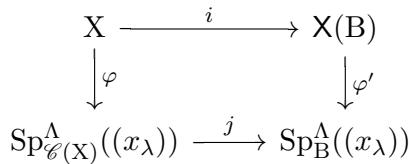
\includegraphics[keepaspectratio]{images/part001_f1662ccb.jpg}}

where \(\varphi\) and \(\varphi'\) are the mappings defined by the family \((x_{\lambda})_{\lambda \in \Lambda}\) (cf. no. 6 of I, p. 41), and \(i\) and \(j\) are the canonical injections. Then:

\begin{enumerate}
\def\labelenumi{\alph{enumi})}
\item
  The maps \(\varphi\) and \(\varphi'\) are homeomorphisms;
\item
  The simultaneous spectrum \(\mathrm{Sp}_{\mathrm{B}}^{\Lambda}((x_{\lambda}))\) is the polynomially convex hull of \(\mathrm{Sp}_{\mathcal{C}(\mathrm{X})}^{\Lambda}((x_{\lambda}))\) ;
\item
  The map \(\varphi\) maps \(\mathcal{C}(\mathrm{X})\) to \(\mathcal{C}(\mathrm{Sp}_{\mathcal{C}(\mathrm{X})}^{\Lambda}((x_{\lambda})))\) and B to \(\mathrm{P}(\mathrm{Sp}_{\mathcal{C}(\mathrm{X})}^{\Lambda}((x_{\lambda})))\) ;
\item
  The map \(\varphi^{\prime}\) maps \(\mathcal{G}_{\mathrm{B}}(\mathrm{B})\) to \(\mathrm{P}(\mathrm{Sp}_{\mathrm{B}}^{\Lambda}((x_{\lambda})))\) ;
\item
  The maps \(\varphi\) and \(\varphi'\) map \(\mathcal{G}_{\mathrm{B}}\) to the canonical isomorphism from \(\mathrm{P}(\mathrm{Sp}_{\mathcal{C}(\mathrm{X})}^{\Lambda}((x_{\lambda})))\) onto \(\mathrm{P}(\mathrm{Sp}_{\mathrm{B}}^{\Lambda}((x_{\lambda})))\) .
\end{enumerate}

The maps \(\varphi\) and \(\varphi'\) are continuous and surjective (I, no. 6, p.~41). The map \(\varphi'\) is a homeomorphism by assertion \(a\) ) of prop. 12 of I, p.~43, and \(i\) is injective, therefore \(\varphi\) is injective. Therefore \(\varphi\) and \(\varphi'\) are homeomorphisms.

Let \(X_{1} = \mathrm{Sp}_{\mathcal{C}(X)}^{\Lambda}((x_{\lambda}))\) . The polynomially convex hull of \(X_{1}\) is \(Y_{1} = \mathrm{Sp}_{\mathrm{B}}^{\Lambda}((x_{\lambda}))\) by prop. 14 of I, p.~46.

For every \(\lambda\in\Lambda\) , let \(z_{\lambda}\) be the corresponding coordinate function on \(\mathbf{C}^{\Lambda}\) . The map \(\varphi\) maps \(x_{\lambda}\) to \(z_{\lambda}|X_{1}\) , and \(\varphi'\) maps \(\mathcal{G}_{\mathrm{B}}(x_{\lambda})\) to \(z_{\lambda}|Y_{1}\) . Therefore \(\varphi\) maps B onto \(\mathrm{P}(X_{1})\) , and \(\varphi'\) maps \(\mathcal{G}_{\mathrm{B}}(B)\) onto \(\mathrm{P}(Y_{1})\) . Finally, \(\varphi\) and \(\varphi'\) map \(\mathcal{G}_{\mathrm{B}}\) to the canonical isomorphism from \(\mathrm{P}(X_{1})\) onto \(\mathrm{P}(Y_{1})\) .

COROLLARY 1. --- Let \(\Lambda\) be a set and X a compact subset of \(\mathbf{C}^{\Lambda}\) . We identify X with a subset of \(\mathsf{X}(\mathrm{P}(\mathrm{X}))\) (prop. 1 of I, p.~142, d)). Let \((z_{\lambda})_{\lambda \in \Lambda}\) be the family of coordinate functions on \(\mathbf{C}^{\Lambda}\) .

\begin{enumerate}
\def\labelenumi{\alph{enumi})}
\item
  The map \(\theta\) from \(\mathrm{X}(\mathrm{P}(\mathrm{X}))\) onto \(\mathrm{Sp}_{\mathrm{P}(\mathrm{X})}^{\Lambda}((z_{\lambda}))\) defined by the family \((z_{\lambda})\) is a homeomorphism from \(\mathrm{X}(\mathrm{P}(\mathrm{X}))\) onto the polynomially convex hull \(Y\) of \(X\). Its restriction to \(X\) is the identity map of \(X\) ;
\item
  For every function \(f \in \mathrm{P}(\mathrm{X})\) , the homeomorphism \(\theta\) transforms the extension \(\mathcal{G}_{\mathrm{P}(\mathrm{X})}(f)\) of \(f\) to \(\mathrm{X}(\mathrm{P}(\mathrm{X}))\) into an extension \(\widetilde{f}\) of \(f\) to \(\mathrm{Y}\) . The map \(f \mapsto \widetilde{f}\) is the canonical isomorphism from \(\mathrm{P}(\mathrm{X})\) onto \(\mathrm{P}(\mathrm{Y})\) .
\end{enumerate}

In prop. 4, take B = P(X) and \(x_{\lambda} = z_{\lambda}\) . Then \(\varphi\) becomes the identity map and \(\varphi'\) becomes the map \(\theta\) . The assertions of the corollary then reduce to those of loc. cit.

COROLLARY 2. --- Let \(\Lambda\) be a set and let \(X \subset \mathbf{C}^{\Lambda}\) be a compact set. If \(X\) is connected, then its polynomially convex hull is connected.

If X is connected, the only idempotents of \(\mathcal{C}(\mathrm{X})\) , hence of \(\mathrm{P}(\mathrm{X})\) , are 0 and 1 (cor. of prop. I, p.~79). Consequently, the space \(\mathrm{X}(\mathrm{P}(\mathrm{X}))\) is connected (loc. cit.); but this set is homeomorphic to the polynomially convex hull of X (cor. 1, a)).

\subsection{Continuous functions on a compact subset of C}

Lemma 1. --- Let X be a compact subset of the plane and let O be a bounded connected component of \(\mathbf{C} - \mathbf{X}\) . The boundary of O is contained in X.

The closure of the set O in C-X is equal to \(\overline{\mathrm{O}}\cap (\mathbf{C} - \mathbf{X})\) where \(\overline{\mathrm{O}}\) is its closure in C. Since O is a connected component of C-X, we therefore have \(\overline{\mathrm{O}}\cap (\mathbf{C} - \mathbf{X}) = \mathrm{O}\) , which indeed proves that \(\overline{\mathrm{O}} -\mathrm{O}\subset \mathrm{X}\) .

Let X be a compact subset of C. Let \(O_{\infty}\) be the unbounded connected component of \(\mathbf{C} - \mathbf{X}\) , and let \((\mathrm{O}_{i})_{i\in\mathrm{I}}\) be the family of bounded connected components of \(\mathbf{C} - \mathbf{X}\) , the sets \(O_{i}\) being pairwise distinct.

Let E be a subset of \(\mathbf{C} - \mathbf{X}\) . We denote by \(\mathrm{R}_{\mathrm{E}}(\mathrm{X})\) the closure in \(\mathcal{C}(\mathrm{X})\) of the set of functions \(f|\mathrm{X}\) , where \(f\) is a rational function on \(\mathbf{C}\) all of whose poles belong to E. The algebra \(\mathrm{R}_{\mathrm{E}}(\mathrm{X})\) is a unital Banach subalgebra of \(\mathcal{C}(\mathrm{X})\) which separates the points of X. Let z be the identity function on X. The full closed subalgebra of \(\mathrm{R}_{\mathrm{E}}(\mathrm{X})\) generated by z is equal to \(\mathrm{R}_{\mathrm{E}}(\mathrm{X})\) (lemma 2 of I, p.~6). The elements of \(\mathrm{R}_{\mathrm{E}}(\mathrm{X})\) are holomorphic in the interior of X.

In particular, we have \(\mathrm{R}_{\varnothing}(\mathrm{X})=\mathrm{P}(\mathrm{X})\) . We denote \(\mathrm{R}(\mathrm{X})=\mathrm{R}_{\mathbf{C}-\mathbf{X}}(\mathrm{X})\) . We denote by I(E) the set of elements \(i\in I\) such that \(E\cap O_{i}=\varnothing\) , and

\[
\mathrm{X} _ {\mathrm{E}} = \mathrm{X} \cup \Big (\bigcup_ {i \in \mathrm{I} (\mathrm{E})} \mathrm{O} _ {i} \Big).
\]

The set \(X_{E}\) is compact, since it is bounded and closed, its complement in \(\mathbf{C}\) being the union of the open \(O_{\infty}\) and open sets \(O_{i}\) that meet E.

PROPOSITION 5. --- With the above notation:

\begin{enumerate}
\def\labelenumi{\alph{enumi})}
\item
  The restriction map h of \(\mathrm{R}_{\mathrm{E}}(\mathrm{X}_{\mathrm{E}})\) into \(\mathrm{R}_{\mathrm{E}}(\mathrm{X})\) is an isometric isomorphism;
\item
  The algebra \(\mathrm{R}_{\mathrm{E}}(\mathrm{X}_{\mathrm{E}})\) is a full subalgebra of \(\mathcal{C}(\mathrm{X}_{\mathrm{E}})\) ;
\item
  Every character of \(\mathrm{R}_{\mathrm{E}}(\mathrm{X}_{\mathrm{E}})\) is of the form \(f \mapsto f(w)\) , where w is an element of \(X_{E}\) ;
\item
  The map \(\chi \mapsto \chi (z)\) is a homeomorphism from \(\mathsf{X}(\mathrm{R}_{\mathrm{E}}(\mathrm{X}))\) onto \(\mathrm{X}_{\mathrm{E}}\) ;
\item
  If E' is a subset of \(\mathbf{C} - \mathbf{X}\) , then we have \(\mathrm{R}_{\mathrm{E}}(\mathrm{X}) = \mathrm{R}_{\mathrm{E}'}(\mathrm{X})\) if and only if \(\mathrm{X}_{\mathrm{E}} = \mathrm{X}_{\mathrm{E}'}\) , which is also equivalent to \(\mathrm{I}(\mathrm{E}) = \mathrm{I}(\mathrm{E}')\) .
\end{enumerate}

The restriction map \(h\) of \(\mathrm{R}_{\mathrm{E}}(\mathrm{X}_{\mathrm{E}})\) into \(\mathrm{R}_{\mathrm{E}}(\mathrm{X})\) is a Banach algebra morphism such that \(\| h(f)\| \leqslant \| f\|\) for every function \(f\in \mathrm{R}_{\mathrm{E}}(\mathrm{X}_{\mathrm{E}})\) . Let \(f\in \mathrm{R}_{\mathrm{E}}(\mathrm{X}_{\mathrm{E}})\) . Let \(i\in \mathrm{I}(\mathrm{E})\) . Since \(f\) is holomorphic in a neighborhood of the bounded open set \(\mathrm{O}_i\) , the maximum principle (VAR, I, p.~29) implies that there exists an element \(z_0\) in the boundary of \(\mathrm{O}_i\) such that \(|f(z_0)| = \sup_{z\in \mathrm{O}_i}|f(z)|\) . Since the boundary of \(\mathrm{O}_i\) is contained in X (lemma 1), it follows that \(\sup_{z\in \mathrm{O}_i}|f(z)|\leqslant \| h(f)\|\) . Since this inequality holds for every \(i\in \mathrm{I}(\mathrm{E})\) , it results that \(\| f\| \leqslant \| h(f)\|\) . The morphism \(h\) is therefore isometric, and in particular injective. Let us now prove that it is surjective. Let \(g\in \mathrm{R}_{\mathrm{E}}(\mathrm{X})\) . There exists a sequence \((f_n)\) of rational functions whose poles belong to E which converges uniformly to \(g\) on X. The \(f_n|\mathrm{X}_{\mathrm{E}}\) are elements of \(\mathrm{R}_{\mathrm{E}}(\mathrm{X}_{\mathrm{E}})\) . Since \(h\) is isometric, the sequence \((f_n|\mathrm{X}_{\mathrm{E}})\) converges in \(\mathcal{C}(\mathrm{X}_{\mathrm{E}})\) . If \(f\) is its limit, we have \(f\in \mathrm{R}_{\mathrm{E}}(\mathrm{X}_{\mathrm{E}})\) and \(g = f|\mathrm{X} = h(f)\) . Hence \(a\) ) .

Let us prove assertion d). Apply prop. 3 of I, p.~144 to the algebra \(B = \mathrm{R}_{\mathrm{E}}(\mathrm{X})\) . Assertion b) of loc. cit. implies that the map which associates \(\chi(z)\) to \(\chi\) is a homeomorphism from \(\mathsf{X}(\mathrm{R}_{\mathrm{E}}(\mathrm{X}))\) onto \(\mathrm{Sp}_{\mathrm{R}_{\mathrm{E}}(\mathrm{X})}(z)\) . Let \(z_{\mathrm{E}}\) be the identity map of \(\mathrm{X}_{\mathrm{E}}\) . By loc. cit., a), we have \(\mathrm{Sp}_{\mathrm{R}_{\mathrm{E}}(\mathrm{X})}(z) = \mathrm{Sp}_{\mathrm{R}_{\mathrm{E}}(\mathrm{X}_{\mathrm{E}})}(z_{\mathrm{E}})\) . It therefore suffices to show that \(\mathrm{Sp}_{\mathrm{R}_{\mathrm{E}}(\mathrm{X}_{\mathrm{E}})}(z_{\mathrm{E}}) = \mathrm{X}_{\mathrm{E}}\) . The corollary of prop. 6 of I, p.~28 shows that \(\mathrm{Sp}_{\mathrm{R}_{\mathrm{E}}(\mathrm{X}_{\mathrm{E}})}(z_{\mathrm{E}})\) is the union of \(\mathrm{Sp}_{\mathcal{C}(\mathrm{X}_{\mathrm{E}})}(z_{\mathrm{E}}) = \mathrm{X}_{\mathrm{E}}\) and of certain bounded connected components of the complement of \(\mathrm{X}_{\mathrm{E}}\) . Let \(\mathrm{O}_{i}\) be one of the bounded connected components of the complement of \(\mathrm{X}_{\mathrm{E}}\) . The intersection \(\mathrm{E} \cap \mathrm{O}_{i}\) is therefore nonempty. Let \(\lambda \in \mathrm{E} \cap \mathrm{O}_{i}\) ; since \((\lambda - z_{\mathrm{E}})^{-1} \in \mathrm{R}_{\mathrm{E}}(\mathrm{X}_{\mathrm{E}})\) , we have \(\lambda \notin \mathrm{Sp}_{\mathrm{R}_{\mathrm{E}}(\mathrm{X}_{\mathrm{E}})}(z_{\mathrm{E}})\) . Thus, \(\mathrm{O}_{i}\) is not contained in \(\mathrm{Sp}_{\mathrm{R}_{\mathrm{E}}(\mathrm{X}_{\mathrm{E}})}(z_{\mathrm{E}})\) . This shows that \(\mathrm{Sp}_{\mathrm{R}_{\mathrm{E}}(\mathrm{X}_{\mathrm{E}})}(z_{\mathrm{E}}) = \mathrm{X}_{\mathrm{E}}\) .

This equality also implies that \(\mathrm{Sp}_{\mathrm{R}_{\mathrm{E}}(\mathrm{X}_{\mathrm{E}})}(z_{\mathrm{E}})=\mathrm{Sp}_{\mathcal{C}(\mathrm{X}_{\mathrm{E}})}(z_{\mathrm{E}})\) . This establishes condition (iii) of prop. 11 of I, p.~41, applied to the canonical injection of \(\mathrm{R}_{\mathrm{E}}(\mathrm{X}_{\mathrm{E}})\) into \(\mathcal{C}(\mathrm{X}_{\mathrm{E}})\) and to the element \(z_{\mathrm{E}}\) . Assertions b) and c) are the equivalent conditions (i) and (ii) of loc. cit.

Assertion \(d\) ) shows that \(\mathrm{X}_{\mathrm{E}} = \mathrm{X}_{\mathrm{E}'}\) if \(\mathrm{R}_{\mathrm{E}}(\mathrm{X}) = \mathrm{R}_{\mathrm{E}'}(\mathrm{X})\) . Conversely, suppose that \(\mathrm{X}_{\mathrm{E}} = \mathrm{X}_{\mathrm{E}'}\) . By replacing \(\mathrm{E}'\) by \(\mathrm{E} \cup \mathrm{E}'\) , we may assume that \(\mathrm{E} \subset \mathrm{E}'\) . According to \(b\) ), the algebra \(\mathrm{R}_{\mathrm{E}}(\mathrm{X}_{\mathrm{E}})\) is a full closed subalgebra of \(\mathcal{C}(\mathrm{X}_{\mathrm{E}})\) , and therefore also of \(\mathrm{R}_{\mathrm{E}'}(\mathrm{X}_{\mathrm{E}})\) . It contains \(z_{\mathrm{E}}\) , and hence \(\mathrm{R}_{\mathrm{E}}(\mathrm{X}_{\mathrm{E}}) = \mathrm{R}_{\mathrm{E}'}(\mathrm{X}_{\mathrm{E}})\) . Applying \(a\) ), we deduce that \(\mathrm{R}_{\mathrm{E}}(\mathrm{X}) = \mathrm{R}_{\mathrm{E}'}(\mathrm{X})\) . Finally, the equivalence of \(\mathrm{X}_{\mathrm{E}} = \mathrm{X}_{\mathrm{E}'}\) and \(\mathrm{I}(\mathrm{E}) = \mathrm{I}(\mathrm{E}')\) is a consequence of the definitions.

COROLLARY 1. --- The following conditions are equivalent:

\begin{enumerate}
\def\labelenumi{(\roman{enumi})}
\item
  The set E meets every bounded connected component of \(\mathbf{C} - \mathbf{X}\) ;
\item
  The map \(\chi \mapsto \chi (z)\) is a homeomorphism from \(\mathsf{X}(\mathrm{R}_{\mathrm{E}}(\mathrm{X}))\) onto \(\mathrm{X}\) ;
\item
  We have \(\mathrm{R_E(X)} = \mathrm{R(X)}\) .
\end{enumerate}

Let \(E' = \mathbf{C} - \mathbf{X}\) . Conditions (i), (ii), and (iii) are respectively equivalent to \(\mathrm{I}(\mathrm{E}) = \mathrm{I}(\mathrm{E}')\) , to \(\mathrm{X}_{\mathrm{E}} = \mathrm{X}_{\mathrm{E}'}\) (by prop. 5, d)) and to \(\mathrm{R}_{\mathrm{E}}(\mathrm{X}) = \mathrm{R}_{\mathrm{E}'}(\mathrm{X})\) . They are therefore equivalent to each other by prop. 5, e).

The following corollary makes the Runge theorem more precise (th. 3 of I, p.~69).

COROLLARY 2 (Runge's theorem). --- For every \(i \in I\) , let \(\lambda_{i}\) be a point of \(O_{i}\) . Let f be a complex function holomorphic in an open neighborhood of X. Then \(f|X\) is the uniform limit on X of restrictions of rational functions whose poles are among the \(\lambda_{i}\) .

With \(E = \{\lambda_{i}\}_{i \in I}\) , the hypothesis is condition (i) of Cor. 1. We therefore have \(\mathrm{R}_{\mathrm{E}}(\mathrm{X}) = \mathrm{R}(\mathrm{X})\) , and Th. 3 of I, p.~69 shows that \(\mathrm{R}(\mathrm{X}) = \mathcal{O}(\mathrm{X})\) .

\exercisesection{Spectra and Characters}


\begin{enumerate}
\def\labelenumi{\arabic{enumi})}
\item
  Let \((e_{1}, e_{2})\) be the canonical basis of \(R^{2}\) and let u be the element of A = \(\mathcal{L}(\mathbf{R}^{2})\) defined by \(u(e_{1}) = e_{2}\) , \(u(e_{2}) = -e_{1}\) . Prove that \(\mathrm{Sp}_{\mathrm{A}}(u) = \varnothing\) and \(\mathrm{Sp}_{\mathrm{A}}(u^{2}) = \{-1\}\) .
\item
  Let \(\mu\) be the Lebesgue measure on \([0,1]\) , H the Hilbert space \(\mathrm{L}_{\mathbf{C}}^{2}([0,1],\mu)\) , \(\mathrm{A} = \mathcal{L}(\mathrm{H})\) , and \(x \in \mathrm{A}\) the operator which transforms the function \(f(t)\) into the function \(tf(t)\) . Prove that \(\mathrm{Sp}_{\mathrm{A}}(x) = [0,1]\) , but that \(x\) has no eigenvalue.
\item
  \begin{enumerate}
  \def\labelenumii{\alph{enumii})}
  \tightlist
  \item
    Let H be a Hilbert space admitting a countable orthonormal basis \((e_{0}, e_{1}, e_{2}, \ldots)\) , and A = L(H). Let \(u \in \mathcal{L}(H)\) be such that \(u(e_{i}) = e_{i+1}\) for every i. Let \(u' \in \mathcal{L}(H)\) be such that \(u'(e_{i}) = e_{i-1}\) for \(i \geqslant 1\) and \(u'(e_{0}) = 0\) . We have \(u'u = 1\) but \(uu'(e_{0}) = 0\) , so that \(\mathrm{Sp}_{\mathrm{A}}(u'u) \neq \mathrm{Sp}_{\mathrm{A}}(uu')\) .
  \end{enumerate}
\end{enumerate}

\begin{enumerate}
\def\labelenumi{\alph{enumi})}
\setcounter{enumi}{1}
\tightlist
\item
  Let A be a unital Noetherian algebra over a commutative field. If \(x, y \in A\) , one has \(\mathrm{Sp}_{\mathrm{A}}(xy) = \mathrm{Sp}_{\mathrm{A}}(yx)\) (use exerc. 6 of A, VIII, p.~37).
\end{enumerate}

\begin{enumerate}
\def\labelenumi{\arabic{enumi})}
\setcounter{enumi}{3}
\tightlist
\item
  Let A be a commutative algebra over C, I an ideal of A, h the canonical injection of I into A, and S the set of \(\chi \in \mathsf{X}'(\mathsf{A})\) which vanish on I.
\end{enumerate}

\begin{enumerate}
\def\labelenumi{\alph{enumi})}
\item
  \(X'(h)\) is surjective.
\item
  \(\mathsf{X}^{\prime}(h)|(\mathsf{X}^{\prime}(\mathsf{A})-\mathsf{S})\) is a homeomorphism from \(\mathsf{X}^{\prime}(\mathsf{A})-\mathsf{S}\) onto \(\mathsf{X}(\mathsf{I})\) . (Let \(\chi_{0}\in\mathsf{X}^{\prime}(\mathsf{A})-\mathsf{S}\) . Let \(x_{1},\ldots,x_{n}\in\mathsf{A}\) , \(\varepsilon>0\) , and let V be the neighborhood of \(\chi_{0}\) in \(\mathsf{X}^{\prime}(\mathsf{A})\) defined by \(|(\chi-\chi_{0})(x_{i})|\leqslant\varepsilon,(i=1,\ldots,n)\) . Let \(u_{0}\in I\) be such that \(\chi_0(u_0) = 1\) . We have \(u_i = u_0x_i \in I\) . Then if \(|(\chi - \chi_0)(u_i)| \leqslant \delta\) ( \(i = 0, 1, \ldots, n\) ) with \(\delta\) small enough, we have \(\chi \in V\) .)
\end{enumerate}

\begin{enumerate}
\def\labelenumi{\arabic{enumi})}
\setcounter{enumi}{4}
\item
  In exerc. 4, take \(A = \mathbf{C}[X,Y]\) and \(I = AX\) . The space X(A) is identified with \(\mathbf{C}^2\) , S = \{0\} is identified with \(\{0\} \times \mathbf{C}\) . Let U be the set of \((\xi, \eta) \in \mathbf{C}^2\) such that \(|\xi| < e^{-|\eta|}\) . Prove that \(X'(h)(U)\) is not a neighborhood of 0 in \(X'(I)\) . Deduce that \(X'(I)\) does not identify with the quotient space of \(X'(A)\) by the equivalence relation defined by \(X'(h)\) . (On this subject, cf.~I, p.~169, exerc. 17.)
\item
  Let A be a commutative algebra over a field and let I be a maximal ideal of A. Prove that we have \(A^{2} \subset I\) with \(\dim(A/I) = 1\) or else that A/I is a field. (Apply to A/I exercise 3 of A, I, p.~153.) In particular, if \(A^{2} = A\) , every maximal ideal of A is regular.
\item
  Let A be a commutative algebra over a commutative field K, \(x \in A\) and \(\alpha \in K\) . The set of \(\chi \in \mathsf{X}(\mathsf{A})\) such that \((\mathcal{G}x)(\chi) = \alpha\) is closed for the Jacobson topology. (Reduce to the case where A has a unit element, then to the case where \(\alpha = 0\) .)
\end{enumerate}

¶ 8) Let A be an algebra, I a two-sided ideal of A, \(\mathrm{J}^{\mathrm{I}}(\mathrm{A})\) the set of primitive ideals of A that do not contain I, and \(\widehat{A}^{I}\) the set of irreducible representations \(\pi \in \widehat{A}\) such that \(\pi(I) \neq 0\) .

\begin{enumerate}
\def\labelenumi{\alph{enumi})}
\item
  If \(\pi \in \widehat{\mathrm{A}}^{\mathrm{I}}\) , one has \(\pi | \mathrm{I} \in \widehat{\mathrm{I}}\) (lemma 5, \(a\) ) of I, p.~12). If representations \(\pi\) and \(\pi' \in \widehat{\mathrm{A}}\) are such that \(\pi | \mathrm{I}\) and \(\pi'|\mathrm{I}\) are equivalent, then \(\pi\) and \(\pi'\) are equivalent. (One may assume that \(\pi(x) = \pi'(x)\) for all \(x \in \mathrm{I}\) . Then, for every \(y \in \mathrm{A}\) , \(\pi(y)\) and \(\pi'(y)\) coincide on \(\sum_{x \in \mathrm{I}} \operatorname{Im} \pi(x)\) , and this subspace is equal to the space of \(\pi\) .)
\item
  If \(\pi \in \widehat{\mathrm{I}}\) , \(\pi\) extends to an element of \(\widehat{\mathrm{A}}^{\mathrm{I}}\) . (Let R be a maximal regular left ideal of I. Let \(g\) be a right unit of I modulo R. Assuming that A admits a unit element, show that the relation \(\mathrm{AR} + \mathrm{A}(1 - g) = \mathrm{A}\) would entail \(g^2 \in \mathrm{R}\) . Therefore \(\mathrm{AR} + \mathrm{A}(1 - g)\) is contained in a maximal left ideal M of A. Prove that \(\mathrm{M} \cap \mathrm{I} = \mathrm{R}\) and \(\mathrm{M} + \mathrm{I} = \mathrm{A}\) .)
\item
  Deduce from a) and b) that the map \(I'\mapsto I'\cap I\) is a homeomorphism from \(\mathrm{J}^{\mathrm{I}}(\mathrm{A})\) onto \(\mathrm{J}(\mathrm{I})\) , and that the map \(\pi\mapsto\pi|I\) is a homeomorphism from \(\widehat{A}^{I}\) onto \(\widehat{I}\) .
\end{enumerate}
% semantic-fragments: legacy-input-seam
\relax{}
\exercisesection{Normed Algebras}

\begin{enumerate}
\def\labelenumi{\arabic{enumi})}
\tightlist
\item
  Let (A, e) be a unital complex algebra.
\end{enumerate}

\begin{enumerate}
\def\labelenumi{\alph{enumi})}
\tightlist
\item
  For a linear form \(\lambda \in \mathrm{A}^*\) such that \(\lambda(e) = 1\) , the following conditions are equivalent:
\end{enumerate}

\begin{enumerate}
\def\labelenumi{(\roman{enumi})}
\item
  For every \(x \in \operatorname{Ker}(\lambda)\) , one has \(x^2 \in \operatorname{Ker}(\lambda)\) ;
\item
  For every \(x \in \mathbb{A}\) , one has \(\lambda(x^{2}) = \lambda(x)^{2}\) ;
\item
  The kernel of \(\lambda\) is a right ideal of A;
\item
  The linear form \(\lambda\) is a unital morphism from A to C.
\end{enumerate}

(Observe that \(\lambda(x - \lambda(x)e) = 0\) for all \(x\in A\) .)

\begin{enumerate}
\def\labelenumi{\alph{enumi})}
\setcounter{enumi}{1}
\item
  Let \(\lambda \in \mathrm{A}^*\) a linear form such that \(\lambda(1) = 1\) and such that for every \(x \in \mathrm{A}\) , one has \(\lambda(x) \in \mathrm{Sp}_{\mathrm{A}}(x)\) . Let \(x \in \mathrm{Ker}(\lambda)\) such that \(\lambda(x^{2}) \neq 0\) The spectrum of \(x\) is not bounded in \(\mathbf{C}\) . (For \(n \geqslant 2\) integer, consider the polynomial \(p \in \mathbf{C}[\mathrm{X}]\) such that \(p(z) = \lambda((ze - x)^{n})\) for all \(z \in \mathbf{C}\) ; observe that its roots belong to the spectrum of \(x\) and bound their Euclidean norm below in terms of \(|\lambda(x^{2})|\) .)
\item
  Suppose that A is a Banach algebra. For a linear form \(\lambda\) on A to be a unital morphism from A into C, it is necessary and sufficient that \(\lambda(e)=1\) and that \(\lambda(x)\in\mathrm{Sp}_{\mathrm{A}}(x)\) for all \(x\in A\) .
\end{enumerate}

\begin{enumerate}
\def\labelenumi{\arabic{enumi})}
\setcounter{enumi}{1}
\tightlist
\item
  Let \(n \geqslant 0\) be an integer. Let \(A_n\) the commutative complex Banach algebra of functions \(f: [0,1] \to \mathbf{C}\) admitting continuous derivatives in \([0,1]\) up to order \(n\) , equipped with the norm
\end{enumerate}

\[
\| f \| = \sum_ {k = 0} ^ {n} \frac {1}{k !} \sup _ {0 \leqslant t \leqslant 1} | f ^ {(k)} (t) |
\]

(example 4 of I, p.~18). Show that \(A_{n}\) is isomorphic to \(A_{m}\) if, and only if, n = m. (However, according to Example 1 of I, p.~144, these Banach algebras all have the same character space.)

\begin{enumerate}
\def\labelenumi{\arabic{enumi})}
\setcounter{enumi}{2}
\tightlist
\item
  Let G be a group equal to its derived subgroup (A, I, p.~67). For every \(g \in G\) , we denote by \(\ell(g)\) the smallest integer \(k \geqslant 0\) such that there exist pairs \((a_{1}, b_{1}), \ldots, (a_{k}, b_{k})\) into \(G \times G\) satisfying \(g = [a_{1}, b_{1}] \cdots [a_{k}, b_{k}]\) .
\end{enumerate}

\begin{enumerate}
\def\labelenumi{\alph{enumi})}
\item
  The map \(\ell\) is a metric on G.
\item
  For every \(g \in \mathbf{G}\) , the limit
\end{enumerate}

\[
\operatorname{lsc} (g) = \lim _ {n \to + \infty} \frac {\ell (g ^ {n})}{n}
\]

exists. It is called the stable commutator length of g.

\begin{enumerate}
\def\labelenumi{\alph{enumi})}
\setcounter{enumi}{2}
\tightlist
\item
  Let S be a set and \(\mathrm{G} = \mathrm{D}(\mathrm{F}(\mathrm{S}))\) the derived subgroup of the free group generated by S. The group G is equal to its derived subgroup, and for every \(g \in G\) , \(g \neq e\) , one has \(\operatorname{lsc}(g) \geqslant 1/2\) . There exists \(g \in G\) such that \(\operatorname{lsc}(g) = 1/2\) .
\end{enumerate}

\begin{enumerate}
\def\labelenumi{\arabic{enumi})}
\setcounter{enumi}{3}
\tightlist
\item
  Let \(n \geqslant 1\) an integer. We denote \(S(n)\) the largest integer \(k \geqslant 0\) such that, for every set \(X\) of \(n\) real numbers, there exists a subset \(Y \subset X\) of cardinality \(k\) such that the equation \(x + y = z\) has no solution in \(Y\) . We therefore have \(S(n) \leqslant n\) .
\end{enumerate}

\begin{enumerate}
\def\labelenumi{\alph{enumi})}
\tightlist
\item
  Show that the limit
\end{enumerate}

\[
\sigma = \lim _ {n \to + \infty} \frac {\mathrm{S} (n)}{n}
\]

exists.

\begin{enumerate}
\def\labelenumi{\alph{enumi})}
\setcounter{enumi}{1}
\item
  Show that \(\sigma \leqslant 2 / 5\) .
\item
  Show that \(\sigma \geqslant 1 / 3\) .
\end{enumerate}

(One can show that \(\sigma = 1/3\) , cf.~S. EBERHARD, B. GREEN, F. MANNERS, Sets of integers with no large sum-free subset, Annals of Mathematics 180 (2014), 621--652.)

\begin{enumerate}
\def\labelenumi{\arabic{enumi})}
\setcounter{enumi}{4}
\tightlist
\item
  Let A be a commutative ring and \(n \geqslant 1\) an integer. For a matrix \(M = (m_{i,j})\) of type \((n, n)\) with coefficients in A, we call the permanent of M the element
\end{enumerate}

\[
\mathrm{per(M)} = \sum_ {\sigma \in \mathrm{S} _ {n}} m _ {1, \sigma (1)} \dots m _ {n, \sigma (n)}
\]

of A.

Let \(k \geqslant 1\) an integer. We denote \(X_{n,k}\) the set of matrices M of type \((n, n)\) with real coefficients such that each column of M contains k coefficients equal to 1, all the others being zero.

Show that the limit

\[
\lim _ {n \to + \infty} \left(\inf _ {\mathrm{M} \in \mathrm{X} _ {n, k}} \operatorname{per} (\mathrm{M})\right) ^ {1 / n}
\]

exists.

\begin{enumerate}
\def\labelenumi{\arabic{enumi})}
\setcounter{enumi}{5}
\tightlist
\item
  Let \(k \geqslant 1\) an integer. For every integer \(N \geqslant 1\) , we denote by \(S_k(N)\) the largest cardinality of a set \(A \subset \{1, \ldots, N\}\) that does not contain \(k\) elements in arithmetic progression, that is, for any \(n_0 \geqslant 0\) , \(h \geqslant 1\) , \(\ell \geqslant 1\) , if \(\{n_0 + h, n_0 + 2h, \ldots, n_0 + \ell h\} \subset A\) , then \(\ell < k\) .
\end{enumerate}

\begin{enumerate}
\def\labelenumi{\alph{enumi})}
\tightlist
\item
  Show that the limit
\end{enumerate}

\[
s _ {k} = \lim _ {\mathrm{N} \to + \infty} \frac {\mathrm{S} _ {k} (\mathrm{N})}{\mathrm{N}}
\]

exists.

\begin{enumerate}
\def\labelenumi{\alph{enumi})}
\setcounter{enumi}{1}
\tightlist
\item
  Show that \(s_{1}=s_{2}=0\) One can show (“Szemerédi's theorem”, cf.~E. SZEMERÉDI, On sets of integers containing no k elements in arithmetic progression, Acta Arithmetica XXVII, 1975, 199--245) that \(s_{k}=0\) for all \(k\geqslant1\) ; for the case k=3, cf.~exercise 23 of II, p.~270.
\end{enumerate}

\begin{enumerate}
\def\labelenumi{\arabic{enumi})}
\setcounter{enumi}{6}
\tightlist
\item
  Let A be a normed algebra.
\end{enumerate}

\begin{enumerate}
\def\labelenumi{\alph{enumi})}
\tightlist
\item
  Let S be a nonempty bounded subset of A. Show that the limit
\end{enumerate}

\[
\varrho (\mathrm{S}) = \lim _ {n \to + \infty} \sup _ {x \in \mathrm{S} ^ {n}} \| x \| ^ {1 / n}
\]

exists and that \(\varrho(\mathrm{S}) = \varrho(x)\) if S is reduced to a single element x. We say that \(\varrho(\mathrm{S})\) is the spectral radius of the part S.

\begin{enumerate}
\def\labelenumi{\alph{enumi})}
\setcounter{enumi}{1}
\tightlist
\item
  Let N be the set of norms p on A, equivalent to the norm of A, and such that A, equipped with p, is a normed algebra. Let X be a subset of A. For there to exist \(p \in N\) such that \(p(x) \leqslant 1\) for all \(x \in X\) , it is necessary and sufficient that there exist a real number \(c \geqslant 0\) such that
\end{enumerate}

\[
\sup _ {n \geqslant 1} \sup _ {x \in X ^ {n}} \| x \| \leqslant c.
\]

\begin{enumerate}
\def\labelenumi{\alph{enumi})}
\setcounter{enumi}{2}
\tightlist
\item
  Show that
\end{enumerate}

\[
\varrho (\mathrm{S}) = \inf _ {p \in \mathrm{N}} \sup _ {x \in \mathrm{S}} p (x).
\]

\begin{enumerate}
\def\labelenumi{\arabic{enumi})}
\setcounter{enumi}{7}
\item
  Let A be the algebra of continuous complex-valued functions on \(\mathbf{R}\) tending to 0 at infinity, equipped with the norm \(\|f\| = \sup_{t\in\mathbf{R}} |f(t)|\) . Then \(\widetilde{\mathrm{A}}\) is identified with the algebra of continuous complex-valued functions on \(\mathbf{R}\) tending toward a finite limit at infinity. On \(\widetilde{\mathrm{A}}\) , the norm \(\|g\| = \sup_{t\in\mathbf{R}} |g(t)|\) differs from the norm defined in no. 1 of I, p.~15.
\item
  Let A be a normed algebra and \(b = \inf_{x \neq 0} \|x^{2}\|/\|x\|^{2}\) . Then
\end{enumerate}

\[
b \leqslant \inf _ {x \neq 0} \frac {\varrho (x)}{\| x \|} \leqslant \sqrt {b}.
\]

\begin{enumerate}
\def\labelenumi{\arabic{enumi})}
\setcounter{enumi}{9}
\item
  Let A be a normed algebra and \(x, y \in A\) . We have \(\varrho(xy) = \varrho(yx)\) .
\item
  Let H be a Hilbert space of countable type and \((f_{n})_{n\geqslant1}\) an orthonormal basis of H. Let A be the normed algebra \(\mathcal{L}(\mathrm{H})\) . Let \(x\in A\) the element defined by \(x(f_{i})=2^{-i}f_{i+1}\) . Show that x is quasi-nilpotent, but not nilpotent.
\end{enumerate}

\begin{enumerate}
\def\labelenumi{¶ \arabic{enumi})}
\setcounter{enumi}{11}
\tightlist
\item
  Let H be a separable Hilbert space and let \((f_n)_{n \geqslant 1}\) be an orthonormal basis of H. One defines the numbers \((\alpha_m)_{m \geqslant 1}\) by \(\alpha_m = e^{-k}\) if \(m\) is the product of \(2^k\) by an odd number.
\end{enumerate}

\begin{enumerate}
\def\labelenumi{\alph{enumi})}
\tightlist
\item
  Let \(x \in \mathcal{L}(\mathrm{H})\) defined by \(x(f_m) = \alpha_m f_{m+1}\) for \(m \geqslant 1\) Prove that \(x\) is not quasi-nilpotent. (Observe that
\end{enumerate}

\[
\left\| x ^ {n} \right\| = \sup _ {m} \bigl (\alpha_ {m} \alpha_ {m + 1} \dots \alpha_ {m + n - 1} \bigr),
\]

and evaluate \(\alpha_{1}\alpha_{2}\ldots\alpha_{2^{t}-1}\) .)

\begin{enumerate}
\def\labelenumi{\alph{enumi})}
\setcounter{enumi}{1}
\tightlist
\item
  Let \(x_{k} \in \mathcal{L}(\mathrm{H})\) defined by \(x_{k}(f_{m}) = 0\) if m is the product of \(2^{k}\) by an odd number, and \(x_{k}(f_{m}) = \alpha_{m} f_{m+1}\) otherwise. Show that \(x_{k}\) is nilpotent and that \((x_{k})\) converges to x as k tends to \(+\infty\) .
\end{enumerate}

\begin{enumerate}
\def\labelenumi{\arabic{enumi})}
\setcounter{enumi}{12}
\item
  Let A be a unital Banach algebra. Let \(x \in A\) such that \(\|x - 1\| < 1\) . There exists \(y \in A\) such that \(y^{2} = x\) .
\item
  Let A be a unital complex normed algebra. If \(\|x^{-1}\| = \|x\|^{-1}\) for every invertible element x of A, one has A = C · 1. (Reduce to the case where A is complete. Let \(x \in A\) , at a distance \(\alpha > 0\) from C · 1. If \(\lambda_{0} \in C\) is such that \(x - \lambda_{0}\) were invertible, then \(x - \lambda\) would be invertible for \(|\lambda - \lambda_{0}| < \alpha\) . Deduce that the spectrum of x would be empty.)
\item
  Let A be a unital complex normed algebra in which the only left topological divisor of zero is 0 and the only right topological divisor of zero is 0. Then \(A = C \cdot 1\) . (If \(x \in A\) , and if \(\lambda\) belongs to the boundary of \(\mathrm{Sp}_{\widehat{\mathrm{A}}}(\boldsymbol{x})\) , then \(x - \lambda\) is a topological divisor of zero in \(\widehat{A}\) , hence in A, therefore \(x = \lambda\) .)
\item
  Let A be a unital complex Banach algebra. Let \(a\) an element of A. The singular spectrum of A is called the set of \(\lambda \in \mathbf{C}\) such that \(a - \lambda e\) is a topological zero divisor on the left and on the right in A.
\end{enumerate}

\begin{enumerate}
\def\labelenumi{\alph{enumi})}
\item
  Show that the singular spectrum of A is contained in the spectrum of A, and contains the boundary of the spectrum of A.
\item
  Let \(f \in C[X]\) a polynomial. The image under f of the singular spectrum of a is the singular spectrum of \(f(a)\) .
\end{enumerate}

\begin{enumerate}
\def\labelenumi{\arabic{enumi})}
\setcounter{enumi}{16}
\tightlist
\item
  Let A be a normed algebra. For every \(x \in A\) , we set:
\end{enumerate}

\[
\lambda (x) = \inf _ {y \neq 0} \frac {\| x y \|}{\| y \|} \quad \lambda^ {\prime} (x) = \inf _ {y \neq 0} \frac {\| y x \|}{\| y \|}.
\]

\begin{enumerate}
\def\labelenumi{\alph{enumi})}
\tightlist
\item
  We have
\end{enumerate}

\[
| \lambda (x) - \lambda (y) | \leqslant \| x - y \|, \quad | \lambda^ {\prime} (x) - \lambda^ {\prime} (y) | \leqslant \| x - y \|,
\]

\[
\lambda (x) \lambda (y) \leqslant \lambda (x y) \leqslant \| x \| \lambda (y), \quad \lambda^ {\prime} (x) \lambda^ {\prime} (y) \leqslant \lambda^ {\prime} (x y) \leqslant \lambda^ {\prime} (x) \| y \|.
\]

\begin{enumerate}
\def\labelenumi{\alph{enumi})}
\setcounter{enumi}{1}
\tightlist
\item
  The set of left (resp. right) topological zero divisors in A is closed.
\end{enumerate}

\begin{enumerate}
\def\labelenumi{\arabic{enumi})}
\setcounter{enumi}{17}
\item
  Let A be a unital Banach algebra. The set of \(x\) which are neither invertible nor topological zero divisors, is open in A.
\item
  Let X be a complex Banach space and \(x \in A = \mathcal{L}(X)\) .
\end{enumerate}

\begin{enumerate}
\def\labelenumi{\alph{enumi})}
\tightlist
\item
  If x is not invertible, then x is a left or right topological zero divisor. (Consider successively the following cases:)
\end{enumerate}

\(1^{\circ}\) ) \(x\) is not injective;

\(2^{\circ})\overline{x(\mathrm{X})}\neq \mathrm{X};\)

\(3^{\circ}) x \text{ is injective, } x(\mathrm{X}) \text{ is dense in X and distinct from X.}\)

\begin{enumerate}
\def\labelenumi{\alph{enumi})}
\setcounter{enumi}{1}
\tightlist
\item
  If x maps X bicontinuously onto a closed vector subspace of X distinct from X, or if x is non-injective with image X, then x is interior to the set of non-invertible elements of A.
\end{enumerate}

\begin{enumerate}
\def\labelenumi{\arabic{enumi})}
\setcounter{enumi}{19}
\item
  In the algebra A of Example 9 of I, p.~20, the identity function z is neither invertible nor a topological zero divisor.
\item
  Let A be a unital normed algebra. Let B be the normed algebra \(\mathcal{L}(\mathrm{A})\) . Then the image of A under the morphism \(x \mapsto \gamma_x\) is a full subalgebra of B. Therefore, if \(x \in \mathrm{A}\) , one has \(\mathrm{Sp}_{\mathrm{A}}(x) = \mathrm{Sp}_{\mathrm{B}}(\gamma_x)\) .
\end{enumerate}

\begin{enumerate}
\def\labelenumi{¶ \arabic{enumi})}
\setcounter{enumi}{21}
\tightlist
\item
  Let A be a Banach algebra.
\end{enumerate}

\begin{enumerate}
\def\labelenumi{\alph{enumi})}
\tightlist
\item
  Let S be the set of bounded sequences of elements of A, with the norm \(\|(\boldsymbol{x}_{n})\| = \sup \|x_{n}\|\) . Let R be the set of \((x_{n}) \in \mathrm{S}\) such that \(\|x_{n}\|\) tends to 0. Then S is a Banach algebra and R is a closed two-sided ideal of S.
\end{enumerate}

Let \(S' = \text{S/R}\) and \(\varphi: \text{S} \to \text{S}'\) the canonical homomorphism.

\begin{enumerate}
\def\labelenumi{\alph{enumi})}
\setcounter{enumi}{1}
\item
  The map \(\theta\) from A into S' defined by \(\theta(x) = \varphi(x, x, x, \ldots)\) is an isometric isomorphism of A onto a subalgebra of S'. Every left topological divisor of zero in S' is a left divisor of zero. For \(x \in A\) to be a left topological divisor of zero, it is necessary and sufficient that \(\theta(x)\) be a left divisor of zero in S'.
\item
  Assume that A has a unit element. Prove that there exists a Banach algebra B and an isometric isomorphism of A onto a subalgebra of B such that an element of A is non-invertible if and only if its image in B is a left or right divisor of zero. (Use (a) and Exercises 19 and 21.)
\end{enumerate}

\begin{enumerate}
\def\labelenumi{\arabic{enumi})}
\setcounter{enumi}{22}
\tightlist
\item
  Let A be a normed algebra and R its radical.
\end{enumerate}

\begin{enumerate}
\def\labelenumi{\alph{enumi})}
\item
  If \(x \in R\) , then x is quasi-nilpotent. (We have \(\mathrm{Sp}_{\mathrm{A}}^{\prime}(x) = \{0\}\) and a fortiori \(\mathrm{Sp}_{\widehat{\mathrm{A}}}^{\prime}(x) = \{0\}\) .)
\item
  Suppose that A is a Banach algebra. Let I be a left ideal of A all of whose elements are quasi-nilpotent. Then \(I \subset R\) (We may assume that A has a unit element. If \(x \in R\) and \(a \in A\) , one has \(\mathrm{Sp}_{\mathrm{A}}(ax) = \{0\}\) , hence 1 - ax is invertible; hence \(x \in R\) .
\end{enumerate}

\begin{enumerate}
\def\labelenumi{\arabic{enumi})}
\setcounter{enumi}{23}
\item
  Let A be a complex Banach algebra, B a complex algebra without radical, and \(\varphi\) a morphism from A onto B. The kernel of \(\varphi\) is closed.
\item
  Let A be a complex Banach algebra and \(\pi\) a nonzero irreducible representation of A in a complex vector space X. Let \(\xi_{0}\) be a nonzero element of X.
\end{enumerate}

\begin{enumerate}
\def\labelenumi{\alph{enumi})}
\item
  The annihilator I of \(\xi_0\) is a maximal regular left ideal of A; it is closed.
\item
  The map \(x \mapsto x\xi_{0}\) defines, by passage to the quotient, an isomorphism \(\varphi\) of the A-module A/I onto the A-module X.
\item
  If one transports by \(\varphi\) the norm of the Banach space A/I, then X becomes a Banach space, and \(\| \pi (x)\| \leqslant \| x\|\) for all \(x\in \mathrm{A}\) .
\item
  If A is primitive (that is, \(\{0\}\) is a primitive ideal, cf. definition I, p. 11, cf. also A, VIII, p. 433, exerc. 6), then \(A = \{0\}\) or \(C \cdot 1\) according as A does or does not have a unit element. (Use the preceding and cor. 4 of I, p. 26).
\end{enumerate}

\begin{enumerate}
\def\labelenumi{¶ \arabic{enumi})}
\setcounter{enumi}{25}
\tightlist
\item
  Let A be a Banach algebra and R its radical.
\end{enumerate}

\begin{enumerate}
\def\labelenumi{\alph{enumi})}
\tightlist
\item
  Prove that if \(r \in R\) , the series
\end{enumerate}

\[
- \frac {1}{2} \sum_ {k = 1} ^ {\infty} \binom{1 / 2}{k} (- 4 r) ^ {k}
\]

converges to an element \(x \in R\) such that \(x^{2} - x + r = 0\) .

\begin{enumerate}
\def\labelenumi{\alph{enumi})}
\setcounter{enumi}{1}
\tightlist
\item
  Let u be an element of A whose class in A/R is idempotent. There exists an idempotent of A congruent to u modulo R. (We may assume that A has a unit element. Let \(q = u - u^{2} \in R\) and \(x \in R\) a solution, constructed with the aid of a), of \(x^{2} - x - q(1 - 4q)^{-1} = 0\) . Then \(u - (2u - 1)x\) answers the question.)
\end{enumerate}

\begin{enumerate}
\def\labelenumi{\arabic{enumi})}
\setcounter{enumi}{26}
\item
  Let A be a complex unital Banach algebra, \(x \in A\) and \(\zeta\) a boundary point of \(\mathrm{Sp}_{\mathrm{A}}(x)\) . The resolvent of x cannot be extended to a continuous function at \(\zeta\) .
\item
  Let A be a complex unital Banach algebra, \(\Delta\) an open subset of C and \(\lambda \mapsto \mathrm{R}(\lambda)\) a map of \(\Delta\) to A such that
\end{enumerate}

\[
\mathrm{R} (\lambda) - \mathrm{R} (\mu) = - (\lambda - \mu) \mathrm{R} (\lambda) \mathrm{R} (\mu)\tag{5}
\]

for all \(\lambda,\mu\in\Delta\) .

\begin{enumerate}
\def\labelenumi{\alph{enumi})}
\tightlist
\item
  Let \(\lambda_0\in \Delta\) . For every \(\lambda \in \Delta\) such that \(|\lambda -\lambda_0|\cdot \| \mathrm{R}(\lambda)\| <  1\) , we have:
\end{enumerate}

\[
\mathrm{R} (\lambda) = \sum_ {n = 0} ^ {\infty} (\lambda_ {0} - \lambda) ^ {n} \mathrm{R} (\lambda_ {0}) ^ {n + 1}.
\]

\begin{enumerate}
\def\labelenumi{\alph{enumi})}
\setcounter{enumi}{1}
\tightlist
\item
  For every \(\lambda \in \Delta\) and every integer \(n\geqslant 0\) , one has
\end{enumerate}

\[
\frac {\partial^ {n}}{\partial \lambda^ {n}} \mathrm{R} (\lambda) = (- 1) ^ {n} n! \mathrm{R} (\lambda) ^ {n + 1}.
\]

\begin{enumerate}
\def\labelenumi{\alph{enumi})}
\setcounter{enumi}{2}
\tightlist
\item
  If R is holomorphic at infinity, then there exists \(z, j, x \in \mathrm{A}\) such that \(z^2 = 0\) , \(j^2 = j\) , \(zj = jz = 0\) , \(x \in j\mathrm{Aj}\) , and \(\mathrm{R}(\lambda) = z + j\mathrm{R}(\lambda, x)\) for \(|\lambda|\) sufficiently large. (Write \(\mathrm{R}(\lambda) = \sum_{n=0}^{\infty} c_n \lambda^{-n}\) for \(|\lambda| > \lambda_0\) , and express that R satisfies (5). One may set \(c_0 = z\) , \(c_1 = j\) , \(c_2 = x\) .)
\end{enumerate}

\begin{enumerate}
\def\labelenumi{\alph{enumi})}
\setcounter{enumi}{3}
\tightlist
\item
  For there to exist \(a \in A\) such that \(R\) is the restriction to \(\Delta\) of the resolvent \(\lambda \mapsto R(a, \lambda)\) of \(a\) , it is necessary and sufficient that there exist \(\lambda_0 \in \Delta\) such that \(R(\lambda_0)\) be invertible.
\end{enumerate}

\begin{enumerate}
\def\labelenumi{\alph{enumi})}
\setcounter{enumi}{4}
\tightlist
\item
  For every \(x \in A\) , the function \(\lambda \mapsto \sum_{n=0}^{\infty} (\lambda_0 - \lambda)^n x^{n+1}\) satisfies (5) for \(|\lambda - \lambda_0| \cdot \|x\| < 1\) .
\end{enumerate}

\begin{enumerate}
\def\labelenumi{\arabic{enumi})}
\setcounter{enumi}{28}
\tightlist
\item
  \begin{enumerate}
  \def\labelenumii{\alph{enumii})}
  \tightlist
  \item
    Let E be a complex Banach space, \(f: \mathbf{C} \to \mathbf{E}\) an entire function and \(\theta \mapsto \mathrm{P}(\theta) = \sum_{\mu=k}^{m} c_{\mu} e^{\mu i\theta}\) a trigonometric polynomial ( \(c_k \neq 0\) ). We assume that \(|\mathrm{P}(\theta)| \cdot \|f(re^{i\theta})\| \leqslant \mathrm{Mr}^{\alpha}\) for \(r \geqslant r_0\) (M, \(r_0\) , \(\alpha\) being constants \(\geqslant 0\) ). Then \(f\) is a polynomial of degree \(\leqslant \alpha\) . (Let \(f(\zeta) = \sum_{\nu=0}^{\infty} a_{\nu} \zeta^{\nu}\) , and
  \end{enumerate}
\end{enumerate}

\[
\mathrm{J} (r, p) = r ^ {- p} \int_ {0} ^ {2 \pi} \mathrm{P} (\theta) f (r e ^ {i \theta}) e ^ {- (k + p) i \theta} d \theta .
\]

Compute the limit of \(\mathrm{J}(r,p)\) when \(r\to+\infty\) in two different ways for \(p>\alpha.\)

\begin{enumerate}
\def\labelenumi{\alph{enumi})}
\setcounter{enumi}{1}
\tightlist
\item
  With the notations of \(a\) ), if \(\alpha\) is an integer and if, for every \(\theta \in \mathbf{R}\) , one has
\end{enumerate}

\[
\lim _ {r \to + \infty} r ^ {- \alpha} | \mathrm{P} (\theta) | \| f (r e ^ {i \theta}) = 0,
\]

then \(f\) is a polynomial of degree \(< \alpha\) .

\begin{enumerate}
\def\labelenumi{\alph{enumi})}
\setcounter{enumi}{2}
\tightlist
\item
  Let A be a unital complex Banach algebra and x a quasi-nilpotent element of A. We assume that, for some integer n \textgreater{} 0, and for every \(\theta \in R\) , one has
\end{enumerate}

\[
\lim _ {r \to + \infty} r ^ {- n} | \cos^ {n} \theta | \cdot \| (1 - r e ^ {i \theta} x) ^ {- 1} \| = 0.
\]

Then \(x^n = 0\) . (Use \(b\) ).)

\begin{enumerate}
\def\labelenumi{¶ \arabic{enumi})}
\setcounter{enumi}{29}
\tightlist
\item
  a) Let E be a complex Banach space and \(x: \mathbf{C}=\{1\}\to\mathrm{E}\) an entire function of \(1/(\zeta-1)\) . One denotes by \(x(\zeta)=\sum_{n=0}^{\infty}a_{n}\zeta^{n}\) , \(x(\zeta)=\sum_{n=0}^{\infty}b_{n}\zeta^{-n}\) the expansions of \(x\) for \(|\zeta|<1\) , \(|\zeta|>1\) respectively. We assume that there exists \(\alpha>0\) such that \(\|a_{n}\|=o(n^{\alpha})\) , \(\|b_{n}\|=o(n^{\alpha})\) . Then \(x(\zeta)\) is a polynomial in \(1 / (\zeta - 1)\) of degree \(< \alpha + 1\) . (Let \(\varepsilon > 0\) . We have \(\|x(\zeta)\| \leqslant \varepsilon(1 - r)^{-1 - \alpha}\) for \(r_{\varepsilon} \leqslant r = |\zeta| < 1\) , \(\|x(\zeta)\| \leqslant \varepsilon(1 - r^{-1})^{-1 - \alpha}\) for \(1 < r \leqslant r_{\varepsilon}'\) . Setting \(1 - \zeta = (\omega + \frac{1}{2})^{-1}\) , \(\omega = \mathrm{Re}^{i\theta}\) , show that, for \(0 \leqslant r < 1\) and \(\mathrm{R} \geqslant 1\) , one has
\end{enumerate}

\[
(1 - r) ^ {- 1} \leqslant \frac {9}{4} \frac {\mathrm{R}}{\cos \theta}
\]

and that, for 1 \textless{} r and R ≥ 1,

\[
(1 - r ^ {- 1}) ^ {- 1} \leqslant \frac {9}{4} \frac {\mathrm{R}}{\cos \theta}.
\]

Set \(y(\omega) = x(\zeta)\) and show that \(R^{-\alpha - 1}|\cos \theta|^{\alpha + 1}\| y(Re^{i\theta})\|\) tends to 0 as \(R\) tends to \(+\infty\) , uniformly in \(\theta\) . Then apply exerc. 29, b).

Let A be a complex unital Banach algebra, \(q \in A\) a quasi-nilpotent element and \(x = 1 + q\) .

\begin{enumerate}
\def\labelenumi{\alph{enumi})}
\setcounter{enumi}{1}
\item
  For \(q^{N}=0\) , it is necessary and sufficient that \(\|x^{\pm n}\|=o(n^{N})\) when n tends to \(+\infty\) . (To see that the condition is sufficient, show, by applying a), that \(\mathrm{R}(\lambda,x)\) is a polynomial in \(1/(\lambda-1)\) of degree \(\leqslant N\) . On the other hand, \(\mathrm{R}(\lambda,x)=\sum_{n=0}^{\infty}q^{n}(\lambda-1)^{-n-1}\) .)
\item
  Let R be the radical of A and G a subgroup of the group of invertible elements of A. If, for every \(x \in G\) , one has \(\|x^{n}\| = o(n)\) , \(\|x^{-n}\| = o(n)\) for \(n \to +\infty\) , then the restriction to G of the canonical map \(A \to A/R\) is injective.
\end{enumerate}

\begin{enumerate}
\def\labelenumi{\arabic{enumi})}
\setcounter{enumi}{30}
\tightlist
\item
  \begin{enumerate}
  \def\labelenumii{\alph{enumii})}
  \tightlist
  \item
    Let A be a normed algebra, and x, y two elements of A such that xy - yx = y. Prove that \(y^{n} = 0\) for \(n > 2\|x\|\) . (Use the formula \(xy^{n} - y^{n}x = ny^{n}\) ).
  \end{enumerate}
\end{enumerate}

\begin{enumerate}
\def\labelenumi{\alph{enumi})}
\setcounter{enumi}{1}
\item
  Let L be a finite-dimensional Lie algebra over C. Prove that, if L is not nilpotent, it contains two nonzero elements x, y such that \([x, y] = y\) . (Use the fact that there exists an \(x \in L\) such that \(\operatorname{ad}(x)\) is not nilpotent.)
\item
  Let L be a real or complex finite-dimensional Lie algebra such that the enveloping algebra of L possesses a norm compatible with its algebra structure. Prove that L is nilpotent. (Use a) and b).
\end{enumerate}

\begin{enumerate}
\def\labelenumi{\alph{enumi})}
\setcounter{enumi}{3}
\tightlist
\item
  Let V be a finite-dimensional real or complex vector space, \(\mathfrak{L}\) a Lie subalgebra of \(\mathfrak{gl}(\mathrm{V})\) consisting of nilpotent endomorphisms, and \(x_{1},\ldots ,x_{n}\) elements of \(\mathfrak{L}\) . Let \(\alpha >0\) . Prove that there exists a Hilbert space structure on V such that \(\| x_i\| \leqslant \alpha\) for \(1\leqslant i\leqslant n\) .
\end{enumerate}

\begin{enumerate}
\def\labelenumi{\alph{enumi})}
\setcounter{enumi}{4}
\tightlist
\item
  Let \(\mathfrak{L}\) be a real or complex finite-dimensional nilpotent Lie algebra, and U its enveloping algebra. Prove that there exists on U a norm compatible with its algebra structure. (Using the method of LIE, I, §3, exerc. 5 and §7, exerc. 3, show that there exists a family \((\pi_{\lambda})\) of representations of \(\mathfrak{L}\) in finite-dimensional spaces \(V_{\lambda}\) , having the following property:
\end{enumerate}

for all \(u \in U\) , there exists an \(\lambda\) such that \(\pi_{\lambda}(u) \neq 0\) , and \(\pi_{\lambda}(\mathfrak{L})\) consists, for every \(\lambda\) , of nilpotent endomorphisms. By endowing each \(V_{\lambda}\) with a Hilbert structure furnished by d), one obtains in the Hilbert space V, the Hilbert sum of the \(V_{\lambda}\) , a representation \(\pi\) of L by continuous endomorphisms, whence an injective morphism \(\varphi\) of U into \(\mathcal{L}(V)\) . Set \(\|u\|_{U} = \|\varphi(u)\|\) for all \(u \in U\) ).

\begin{enumerate}
\def\labelenumi{\alph{enumi})}
\setcounter{enumi}{5}
\tightlist
\item
  Let A be a complex unital normed algebra and x and y elements of A. If \(A \neq \{0\}\) , one has xy - yx ≠ 1. (First proof: one has \(\mathrm{Sp}_{\mathrm{A}}^{\prime}(xy) = \mathrm{Sp}_{\mathrm{A}}^{\prime}(yx)\) ; if xy = yx + 1, then \(\mathrm{Sp}_{\mathrm{A}}(xy)\) is deduced from \(\mathrm{Sp}_{\mathrm{A}}(yx)\) by the translation \(z \mapsto z + 1\) ; deduce that \(\mathrm{Sp}_{\mathrm{A}}(xy)\) is unbounded, which is absurd. Second proof: if \([x, y] = 1\) , one has \([xy, y] = y\) , whence \(y^{n} = 0\) for n sufficiently large by a); since \([x, y^{p}] = py^{p-1}\) deduce that y = 0).
\end{enumerate}

\begin{enumerate}
\def\labelenumi{\arabic{enumi})}
\setcounter{enumi}{31}
\item
  Let A be a normed algebra and \(x \in A\) . One says that x is topologically nilpotent if \(x^{n}\) tends to 0 when n tends to \(+\infty\) . Show that x is topologically nilpotent if and only if \(\varrho(x) < 1\) .
\item
  Let A be a commutative unital Banach algebra over C. Suppose that every closed ideal I of A is finitely generated (that is, there exist \(n \in N\) and \(x_{1}, \ldots, x_{n} \in A\) such that \(I = Ax_{1} + \cdots + Ax_{n}\) ).
\end{enumerate}

\begin{enumerate}
\def\labelenumi{\alph{enumi})}
\tightlist
\item
  Every ideal I of A is closed. (Write \(\bar{\mathrm{I}} = \mathrm{A}x_{1} + \dots +\mathrm{A}x_{n}\) with \(x_{1},\ldots ,x_{n}\) in A. Let \((x_{ip})_{p\geqslant 1}\) be a sequence of elements of I tending to \(x_{i}\) . For every \((y_{1},\ldots ,y_{n})\in \mathrm{A}^{n}\) and every \(p\geqslant 1\) , set
\end{enumerate}

\[
\begin{array}{c} \varphi (y _ {1}, \ldots , y _ {n}) = x _ {1} y _ {1} + \dots + x _ {n} y _ {n} \in \bar {\mathrm{I}} \\ \varphi_ {p} (y _ {1}, \ldots , y _ {n}) = x _ {i p} y _ {1} + \dots + x _ {n p} y _ {n} \in \mathrm{I}. \end{array}
\]

We have \(\varphi\in\mathcal{L}(A^{n},\bar{I})\) , \(\varphi_{p}\in\mathcal{L}(A^{n},\bar{I})\) , \(\|\varphi-\varphi_{p}\|\) tends to 0 as \(p\) tends to \(+\infty\) , and \(\varphi\) is surjective. Deduce that \(\varphi_{p}\) is surjective for \(p\) large enough, considering the transposes of \(\varphi\) and \(\varphi_{p}\) Hence I= \(\bar{I}\) .

\begin{enumerate}
\def\labelenumi{\alph{enumi})}
\setcounter{enumi}{1}
\item
  If A is an integral domain, \(A = C \cdot 1\) (Use a) and Exerc. 15.)
\item
  If the only nilpotent element of A is 0, there exists an integer \(n \geqslant 0\) such that A is isomorphic to \(\mathbf{C}^n\) . (Since A is Noetherian, \(\{0\}\) is the intersection of prime ideals \(\mathfrak{p}_1, \ldots, \mathfrak{p}_m\) ; these are closed by \(a\) ), and the algebras \(\mathrm{A}/\mathfrak{p}_i\) are isomorphic to \(\mathbf{C}\) according to \(b\) .)
\end{enumerate}

\begin{enumerate}
\def\labelenumi{\alph{enumi})}
\setcounter{enumi}{3}
\tightlist
\item
  We have \(\dim_{\mathbf{C}}\mathrm{A} < +\infty\) . (Let N be the set of nilpotent elements of A, which is a (closed) ideal of A. Then \(\dim (\mathrm{A / N}) < +\infty\) according to \(c\) ). Since N is a finitely generated ideal, \(\mathrm{N}^n = 0\) for \(n\) sufficiently large. Finally, each \(\mathrm{N}^i /\mathrm{N}^{i + 1}\) is a finitely generated module over A/N, hence \(\dim (\mathrm{N}^i /\mathrm{N}^{i + 1}) < +\infty\) .)
\end{enumerate}

\begin{enumerate}
\def\labelenumi{\arabic{enumi})}
\setcounter{enumi}{33}
\tightlist
\item
  Let A be a unital algebra over C, equipped with a separated locally convex topology such that multiplication in A is separately continuous.
\end{enumerate}

. An element \(a \in A\) is said to be regular if there exists \(r \geqslant 0\) such that \(a - \lambda\) let be invertible for \(|\lambda| \geqslant r\) , and such that the set of \((a - \lambda)^{-1}\) , for \(|\lambda| \geqslant r\) , be bounded.

\begin{enumerate}
\def\labelenumi{\alph{enumi})}
\item
  If a is regular, \(\lambda(a-\lambda)^{-1}\) remains bounded for \(|\lambda|\geqslant r\) .
\item
  If the mapping \(x \mapsto x^{-1}\) is defined in a neighborhood of 1 and continuous at the point 1, every element of A is regular.
\item
  For every \(a \in A\) , let \(U_{a}\) the set of \(\lambda \in C\) such that \((a - \mu)^{-1}\) exists and is bounded for all \(\mu\) of a neighborhood of \(\lambda\) . Let \(S_{a} = C - U_{a}\) . Then \(S_{a}\) is closed; and, if a is regular, \(S_{a}\) is compact nonempty (provided that \(A \neq \{0\}\) ).
\item
  Let \(a \in A\) . The function \(\lambda \mapsto (a - \lambda)^{-1}\) is holomorphic in \(U_{a}\) .
\item
  Let \(a \in A\) . For \(\lambda \in U_{a}\) , it is necessary and sufficient that \(a - \lambda\) has a regular inverse.
\item
  If every element of A is regular, and if A is a field, then we have \(A = C \cdot 1\) .
\end{enumerate}

\begin{enumerate}
\def\labelenumi{\arabic{enumi})}
\setcounter{enumi}{34}
\tightlist
\item
  Let A be an algebra over R which is a field, equipped with a separated locally convex topology such that multiplication in A is continuous, and such that the map \(x \mapsto x^{-1}\) be continuous at 1. Then A is R-isomorphic either to R, to C, or to the quaternion field H. (If A is commutative and there exists \(u \in A\) with \(u^{2} = -1\) give A a structure of algebra over C, and apply exerc. 34, f).) If A is commutative and there exists no element \(u \in A\) such that \(u^{2} = -1\) apply exerc. 34, f) to the field \(A \otimes_{R} C\) If A is noncommutative, argue as in AC, VI, §6, no. 4, th. 1, third case.)
\end{enumerate}

\begin{enumerate}
\def\labelenumi{¶ \arabic{enumi})}
\setcounter{enumi}{35}
\tightlist
\item
  Let A be the algebra over C consisting of the restrictions to {[}0,1{]} of rational functions in one variable with complex coefficients. This algebra is a field.
\end{enumerate}

\begin{enumerate}
\def\labelenumi{\alph{enumi})}
\item
  We endow A with the topology of convergence in measure (INT, IV, §5, no. 11). Then the mappings \((x,y)\mapsto x+y\) and \((x,y)\mapsto xy\) of A × A into A are continuous, and the map \(x\mapsto x^{-1}\) from A* to A is continuous. The topology of A is not locally convex.
\item
  For \(n \in N^{*}\) , we define the sequence \((w_{r,n})_{r \in \mathbf{Z}}\) by \(w_{r,n} = (-r + 1)^{n(-r+1)}\) if r \textless{} 0, \(w_{0,n} = 1\) and \(w_{r,n} = (r + 1)^{-(r+1)/n}\) if r \textgreater{} 0. If \(f \in A\) , set \(p_n(f) = \sum_r w_{r,n} |a_r| < +\infty\) , where \(\sum a_r t^r\) is the Laurent expansion of \(f(t)\) at 0. Then the \(p_n\) are semi-norms that define on A a metrizable locally convex topology. The map \((x, y) \mapsto xy\) The mapping from A × A to A is continuous. The map \(x \mapsto x^{-1}\) The map from A* into A is not continuous. The algebra A is not complete for this topology.
\end{enumerate}

\begin{enumerate}
\def\labelenumi{\arabic{enumi})}
\setcounter{enumi}{36}
\tightlist
\item
  \begin{enumerate}
  \def\labelenumii{\alph{enumii})}
  \tightlist
  \item
    Let A be an algebra over C equipped with a locally convex topology. The following conditions are equivalent:
  \end{enumerate}
\end{enumerate}

\begin{enumerate}
\def\labelenumi{(\roman{enumi})}
\item
  there exists a fundamental system \((\mathrm{U}_{i})\) of convex balanced neighborhoods of 0 such that \(U_{i}U_{i} \subset U_{i}\) for all i ;
\item
  A is isomorphic to a subalgebra of a product of normed algebras.
\item
  the topology of A can be defined by a family of semi-norms \(p_{i}\) satisfying \(p_{i}(xy) \leqslant p_{i}(x)p_{i}(y)\) for all \(x, y \in A\) .
\end{enumerate}

If A satisfies these conditions, we say that A is locally m-convex.

\begin{enumerate}
\def\labelenumi{\alph{enumi})}
\setcounter{enumi}{1}
\item
  Let A be a locally m-convex algebra. The map \((x,y)\mapsto xy\) The mapping from A × A into A is continuous. If A is unital, and if G denotes the set of invertible elements of A, then the map \(x\mapsto x^{-1}\) of G into A is continuous.
\item
  Let A be a unital locally m-convex algebra. The spectrum of every element of A is nonempty. If A is a field, then \(A = C \cdot 1\) .
\item
  Let A be a complete locally m-convex algebra. There exists a directed set I, a family \((\mathrm{A}_{i})_{i\in\mathrm{I}}\) of Banach algebras, continuous morphisms \(\pi_{ij}\colon A_{j}\mapsto A_{i}\) for \(i\leqslant j\) , with \(\pi_{ij}\circ\pi_{jk}=\pi_{ik}\) such that A is isomorphic to the subalgebra of \(\prod_{i}A_{i}\) consisting of \((x_{i})\) such that \(\pi_{ij}(x_{j})=x_{i}\) for \(i\leqslant j\) .
\item
  The algebra \(\mathcal{C}_{\mathbf{C}}(\mathbf{R})\) , equipped with the topology of compact convergence, is locally m-convex. The set of invertible elements of \(\mathcal{C}_{\mathbf{C}}(\mathbf{R})\) is dense in \(\mathcal{C}_{\mathbf{C}}(\mathbf{R})\) ; it is not open.
\item
  Let D be an open subset of C, and let A be the algebra of complex-valued holomorphic functions on D, equipped with the topology of compact convergence. Then A is locally m-convex. The set of invertible elements of A is closed.
\item
  The algebra of infinitely differentiable complex-valued functions on {[}0,1{]}, equipped with the topology of uniform convergence of each derivative, is locally m-convex.
\item
  Let A be the algebra of (classes of) complex functions f on {[}0,1{]} such that \(f \in \mathrm{L}^{p}([0,1])\) for every p \textgreater{} 1. Endowed with the topology defined by the family of seminorms \(f \mapsto \|f\|_{p}\) (p \textgreater{} 1), A is not locally m-convex. The map \((x,y) \mapsto xy\) from A × A into A is continuous.
\end{enumerate}

\exercisesection{Commutative Banach Algebras}

In the exercises below, all algebras considered are over C, unless explicitly stated otherwise.

\begin{enumerate}
\def\labelenumi{\arabic{enumi})}
\item
  Let A be a commutative Banach algebra and I a maximal ideal of A. Show that there are only two possible cases: either I is the kernel of a character of A, or I is a hyperplane containing \(A^{2}\) . (Use exerc. 6 of I, p.~154). In particular, if I is not closed, I is a dense hyperplane of A containing \(A^{2}\) . (To obtain an example of this latter situation, consider exerc. 3.)
\item
  Let A be the Banach algebra of sequences \(x = (x_{n})_{n \geqslant 1}\) of complex numbers tending to 0, with \(\|x\| = \sup_{i} |x_{i}|\) . Let I be the set of elements of A with finite support. Then I is a dense ideal of A, and is contained in no maximal ideal. (Observe that \(A^{2} = A\) , and use exerc. 1.)
\item
  Let \(\Lambda\) a set, \(p \in [1, +\infty[\) , and \(\mathbf{A} = \ell^p(\Lambda)\) the set of families \(x = (x_{\lambda})_{\lambda \in \Lambda}\) , where \(x_{\lambda} \in \mathbf{C}\) and
\end{enumerate}

\[
\| x \| _ {p} = \left(\sum_ {\lambda} | x _ {\lambda} | ^ {p}\right) ^ {1 / p} <   + \infty .
\]

\begin{enumerate}
\def\labelenumi{\alph{enumi})}
\item
  For componentwise addition and multiplication, and the norm \(x \mapsto \| x \|_p\) , the space A is a Banach algebra.
\item
  We have \(A^{2} \neq A\) and \(A^{2}\) is dense in A.
\item
  The space \(\mathsf{X}(\mathsf{A})\) of nonzero characters of A is naturally identified with \(\Lambda\) endowed with the discrete topology. (Use the fact that the dual of \(\ell^{p}(\Lambda)\) is \(\ell^{q}(\Lambda)\) , where q is the conjugate exponent of p.) The Gelfand transformation then becomes the identity map and its image in the space of continuous functions tending to 0 at infinity on \(\Lambda\) is dense and not closed.
\end{enumerate}

\begin{enumerate}
\def\labelenumi{\arabic{enumi})}
\setcounter{enumi}{3}
\tightlist
\item
  Let \((\alpha_{n})_{n\geqslant 0}\) a sequence in \(\mathbf{R}_{+}^{*}\) such that \(\alpha_0 = 1\) , \(\alpha_{m + n}\leqslant \alpha_m\alpha_n\) for all integers \(m\) and \(n\) , and such that \(\alpha_{n}^{1 / n}\to 0\) . Let A be the set of formal series \(x = \sum_{n = 0}^{\infty}x_{n}z^{n}\in \mathbf{C}[[z]]\) such that
\end{enumerate}

\[
\| x \| = \sum_ {n = 0} ^ {\infty} | x _ {n} | \alpha_ {n} <   + \infty .
\]

Show that A is a commutative unital Banach algebra topologically generated by z, and that the unique maximal ideal of A is the set of \(x \in A\) without constant term. (Observe that z is quasi-nilpotent.)

\begin{enumerate}
\def\labelenumi{\arabic{enumi})}
\setcounter{enumi}{4}
\item
  In the algebra \(\mathbf{C}(\mathrm{X})\) of rational fractions over \(\mathbf{C}\) , the ideal \(\{0\}\) is maximal, but is not of codimension 1.
\item
  Let \(\Delta\) the closed unit disk in C. Show that the group of invertible elements in \(\mathcal{C}(\Delta)\) is not dense in \(\mathcal{C}(\Delta)\) .
\item
  Let A be a commutative unital Banach algebra and \(\chi \in \mathsf{X}(\mathsf{A})\) . For every \(x \in \mathsf{A}\) , set \(\|x\|_{\chi} = |\chi(x)| + \|x - \chi(x)\|\) . Show that \(x \mapsto \|x\|_{\chi}\) is a norm, that \(\|xy\|_{\chi} \leqslant \|x\|_{\chi}\|y\|_{\chi}\) , \(\|e\|_{\chi} = 1\) , and that if \(\|e\| = 1\) , then \(\|x\| \leqslant \|x\|_{\chi} \leqslant 3\|x\|\) .
\item
  Let A be a commutative unital Banach algebra such that \(\|1\| = 1\) . Let N be the set of norms equivalent to the given norm, for which A is still a Banach algebra, and for which 1 has norm 1.
\end{enumerate}

\begin{enumerate}
\def\labelenumi{\alph{enumi})}
\tightlist
\item
  Let \(x_{0} \in A\) such that \(\varrho(x_{0}) < 1\) . For every \(x \in A\) , we set:
\end{enumerate}

\[
\left\| x \right\| ^ {\prime} = \inf \sum_ {n} \left\| a _ {n} \right\|
\]

for all representations of \(x\) in the form \(a_0 + a_1 x_0 + \cdots + a_n x_0^n\) (with \(a_0, a_1, \ldots, a_n \in \mathrm{A}\) ). Show that \(x \mapsto \|x\|^{\prime}\) is an element of N. (Since \(\varrho(x_0) < 1\) , there exists \(k\) such that \(\|x_0^n\| \leqslant k\) for all \(n\) , whence \(\|x\| \leqslant k \|x\|^{\prime}\) .)

\begin{enumerate}
\def\labelenumi{\alph{enumi})}
\setcounter{enumi}{1}
\item
  Show that \(\|x_{0}\|^{\prime}\leqslant1\) .
\item
  Deduce from a) and b) that, for every \(x \in A\) , one has
\end{enumerate}

\[
\varrho (x) = \inf _ {n \in \mathrm{N}} n (x).
\]

\begin{enumerate}
\def\labelenumi{\alph{enumi})}
\setcounter{enumi}{3}
\tightlist
\item
  If the only element of N is the given norm, we have \(A = C \cdot 1\) . (Use c) and exerc. 7.)
\end{enumerate}

\begin{enumerate}
\def\labelenumi{\arabic{enumi})}
\setcounter{enumi}{8}
\item
  Let X be a locally compact space and A the Banach algebra \(\mathcal{C}_{0}(X)\) . Let I be an ideal of A such that, for every \(x \in X\) , there exists \(f \in I\) such that \(f(x) \neq 0\) . Show that I contains the ideal of functions with compact support in X.
\item
  Let A be a commutative Banach algebra and D a continuous derivation of A into A, that is, a continuous linear map of A into A such that \(\mathrm{D}(ab)=(\mathrm{Da})b+a(\mathrm{Db})\) for \(a,b\in A\) .
\end{enumerate}

\begin{enumerate}
\def\labelenumi{\alph{enumi})}
\tightlist
\item
  For every \(\chi \in \mathsf{X}'(\mathbf{A})\) and every \(\lambda \in \mathbf{C}\) , the series
\end{enumerate}

\[
\varphi_ {\lambda} (a) = \sum_ {n = 0} ^ {\infty} \frac {\lambda^ {n}}{n !} \chi (\mathrm{D} ^ {n} (a))
\]

converges; \(\lambda \mapsto \varphi_{\lambda}(a)\) is an entire function, and \(a \mapsto \varphi_{\lambda}(a)\) is a character of A.

\begin{enumerate}
\def\labelenumi{\alph{enumi})}
\setcounter{enumi}{1}
\item
  The number \(\varphi_{\lambda}(a)\) is independent of \(\lambda\) . (Observe that \(|\varphi_{\lambda}(a)| \leqslant \|a\|\) according to \(a\) ).) Hence \(\chi(\mathrm{D}(a)) = 0\) .
\item
  The image of D is contained in the radical of A. Deduce from this a new proof of assertion f) of exerc. 31 of I, p.~162.
\end{enumerate}

\begin{enumerate}
\def\labelenumi{\arabic{enumi})}
\setcounter{enumi}{10}
\tightlist
\item
  Let B be the algebra over C of infinitely differentiable functions on {[}0,1{]} in C.
\end{enumerate}

\begin{enumerate}
\def\labelenumi{\alph{enumi})}
\tightlist
\item
  Let A be a subalgebra of B, equipped with a norm making A a Banach algebra. Show that there exists a sequence \((m_{n})_{n\geqslant0}\) into \(R_{+}\) such that, for all \(x\in A\) , one has
\end{enumerate}

\[
\sup _ {0 \leqslant t \leqslant 1} | x ^ {(n)} (t) | = \mathrm{O} (m _ {n}).
\]

(Let \(\mathrm{B}_n\) the Banach algebra of functions \(n\) times continuously differentiable on {[}0,1{]}. By prop. 9 of I, p.~40, the canonical injection \(\mathrm{A} \to \mathrm{B}_n\) is continuous; let \(\mathrm{M}_n\) be its norm; if \(x \in \mathrm{A}\) , one has \(\sup_{0 \leq t \leq 1} |x^{(n)}(t)| \leqslant n!\mathrm{M}_n \| x\|\) .)

\begin{enumerate}
\def\labelenumi{\alph{enumi})}
\setcounter{enumi}{1}
\tightlist
\item
  There exists no norm on B making it a Banach algebra.
\end{enumerate}

\begin{enumerate}
\def\labelenumi{\arabic{enumi})}
\setcounter{enumi}{11}
\tightlist
\item
  Let A be a unital Banach algebra and \((x_{n})\) a sequence of invertible elements of A tending to an element \(x \in A\) If the sequence \((\varrho(x_{n}^{-1}))\) is bounded, and if \(x_{n}x = xx_{n}\) for all n, then x is invertible. (By the cor. of prop. 8 of I, p.~38, \(\varrho(1 - x_{n}^{-1}x) \leqslant \varrho(x_{n}^{-1})\varrho(x_{n} - x)\) , hence \(x_{n}^{-1}x\) is invertible for n sufficiently large.)
\end{enumerate}

\begin{enumerate}
\def\labelenumi{¶ \arabic{enumi})}
\setcounter{enumi}{12}
\tightlist
\item
  Let A be the Banach algebra \(\ell^{2}(\mathbf{N})\) (exerc. 3). Let \(\mathrm{A}_{0}\) the subalgebra formed by sequences with finite support. Let B be the direct sum of \(\mathrm{A}_{0}\) and of \(\mathbf{C}\) , equipped with the multiplication \((f,\alpha)(g,\beta)=(fg,0)\) for \(f,g\in\mathrm{A}_{0},\alpha,\beta\in\mathbf{C}\) , and the norm
\end{enumerate}

\[
\left\| (f, \alpha) \right\| = \sup \left(\left\| f \right\|, \left| \alpha - \sum_ {n} f (n) \right|\right).
\]

\begin{enumerate}
\def\labelenumi{\alph{enumi})}
\item
  The completed algebra \(\widehat{\mathbf{B}}\) is a commutative Banach algebra whose radical R is \(\mathbf{C} \cdot (0,1)\) , and \(\widehat{\mathbf{B}}/\mathbf{R}\) is isometrically isomorphic to A.
\item
  Let \(\pi\colon\widehat{\mathrm{B}}\to\widehat{\mathrm{B}}/\mathrm{R}\) the canonical morphism. There exists no subalgebra \(\mathrm{B}_{1}\) of \(\widehat{\mathrm{B}}\) supplementary to R such that \(\pi|\mathrm{B}_{1}\colon\mathrm{B}_{1}\to\widehat{\mathrm{B}}/\mathrm{R}=\mathrm{A}\) is a homeomorphism. (Let \(\mathrm{B}_{1}\) be such a subalgebra. Let \(u_{n}\in\mathrm{A}\) such that \(u_{n}(n)=1\) , \(u_{n}(m)=0\) for \(m\neq n\) . Let \(e_{n}\in\mathrm{B}_{1}\) such that \(\pi(e_{n})=u_{n}\) . Show that \(e_{n}\in\mathrm{A}_{0}\) , that \(\sum_{n=1}^{\infty}\frac{1}{n}u_{n}\) converges in A but \(\sum_{n=1}^{\infty}\frac{1}{n}e_{n}\) does not converge in \(\widehat{\mathrm{B}}\) .)
\end{enumerate}

\begin{enumerate}
\def\labelenumi{\arabic{enumi})}
\setcounter{enumi}{13}
\tightlist
\item
  In \(\mathbf{C}^2\) , let \(\Omega\) the compact set defined by
\end{enumerate}

\[
\frac {1}{2} \leqslant | z _ {1} | ^ {2} + | z _ {2} | ^ {2} \leqslant 1,
\]

and let A be the subalgebra of \(\mathcal{C}(\Omega)\) consisting of functions that are holomorphic in \(\mathring{\Omega}\) . Let U be the open set defined by \(|z_1|^2 + |z_2|^2 < 1\) . By virtue of a theorem of Hartogs (cf.~J.-P. DEMAILLY, Complex analytic and differential geometry, Ch. I, th. 3.28), for every \(f \in \mathrm{A}\) , there exists a function \(\widetilde{f} \in \mathcal{C}(\overline{\mathrm{U}})\)

, unique, which is holomorphic in U and coincides with f on \(\Omega\) . Show that the canonical injection from A into \(\mathcal{C}(\Omega)\) is an isometric morphism h whose image is a full subalgebra of \(\mathcal{C}(\Omega)\) but \(\mathsf{X}(h)\) is not surjective.

\begin{enumerate}
\def\labelenumi{\arabic{enumi})}
\setcounter{enumi}{14}
\item
  Let A and B be commutative unital Banach algebras, \(\varphi\) a unital morphism from A to B and \((x_{\lambda})_{\lambda \in \Lambda}\) a family of elements of A such that the closed full subalgebra of A generated by the \(x_{\lambda}\) is equal to A. For \(\mathsf{X}(\varphi)\) to be surjective, it is necessary and sufficient that \(\mathrm{Sp}_{\mathrm{A}}^{\Lambda}((x_{\lambda})) = \mathrm{Sp}_{\mathrm{B}}^{\Lambda}((\varphi (x_{\lambda})))\) (Use diagram (1) of no. 6 of I, p.~41, where the right-hand arrow is bijective by prop. 12 of I, p.~43.)
\item
  Let A be a commutative Banach algebra. The following conditions are equivalent:
\end{enumerate}

\begin{enumerate}
\def\labelenumi{(\roman{enumi})}
\item
  A is radical-free and \(\mathcal{G}(\mathrm{A})\) is closed in \(\mathcal{C}_0(\mathsf{X}(\mathrm{A}))\) ;
\item
  \(\mathcal{G}\) is a homeomorphism from A onto \(\mathcal{G}(\mathrm{A})\) ;
\item
  there exists a constant c \textgreater{} 0 such that \(\|x\|^{2} \leqslant c\|x^{2}\|\) for all \(x \in A\) .
\end{enumerate}

\begin{enumerate}
\def\labelenumi{\arabic{enumi})}
\setcounter{enumi}{16}
\item
  Let A be a commutative Banach algebra and I a closed ideal of A. Denote by h the canonical injection of I into A. The space \(\mathsf{X}'(\mathsf{I})\) is identified with the quotient space of \(\mathsf{X}'(\mathsf{A})\) by the equivalence relation defined by \(\mathsf{X}'(h)\) . (Use part (a) of Exercise 4 of I, p.~153).
\item
  Let A be a unital commutative Banach algebra and \(x\) an element of A. Suppose that the closed full subalgebra of A generated by \(x\) is equal to A, so that the map \(\chi \mapsto \chi(x)\) allows one to identify \(\mathsf{X}(\mathsf{A})\) and \(\mathrm{Sp}_{\mathsf{A}}(x)\) . Let \(\mathcal{H}\) the set of functions \(\mathcal{G}y\) on \(\mathrm{Sp}_{\mathsf{A}}(x)\) , for \(y\) ranging over A. Then \(\check{\mathrm{S}}_{\mathcal{H}}(\mathrm{Sp}_{\mathsf{A}}(x))\) (INT, IV, §7, no. 4) is the boundary of \(\mathrm{Sp}_{\mathsf{A}}(x)\) relative to C. (To show that \(\check{\mathrm{S}}_{\mathcal{H}}(\mathrm{Sp}_{\mathsf{A}}(x))\) is contained in this boundary, use the maximum principle. Conversely, let \(z_0\) a point of this boundary; to show that \(z_0 \in \check{\mathrm{S}}_{\mathcal{H}}(\mathrm{Sp}_{\mathsf{A}}(x))\) , consider \((x - z_1)^{-1}\) for \(z_1\) quite close to \(z_0\) into \(\mathbf{C} = \mathrm{Sp}_{\mathsf{A}}(x)\) .)
\item
  Let A be a commutative unital Banach algebra, B a closed unital subalgebra of A, and T the map \(\chi \mapsto \chi|B\) from X(A) into X(B), and let R be the equivalence relation on X(A) defined by T. Then T induces, by passing to the quotient, a homeomorphism from X(A)/R onto T(X(A)), and for every \(x \in B\) , the function \(f = \mathcal{G}_{\mathrm{B}}(x)\) is such that \(|f|\) attains its upper bound on T(X(A)).
\item
  Let \(\Delta\) the disk \(|z| \leqslant 1\) into \(\mathbf{C}\) the set of \(f \in \mathcal{C}(\Delta)\) that are holomorphic in the interior of \(\Delta\) and \(\mathrm{A}_1\) the Banach subalgebra of \(\mathcal{C}(\Delta)\) generated by A and by the function \(z \mapsto |z|\) . Show that \(\mathrm{X}(\mathrm{A}_1)\) is homeomorphic to the set of \((x_{1}, x_{2}, x_{3}) \in \mathbf{R}^{3}\) such that \(x_{1}^{2} + x_{2}^{2} \leqslant x_{3}^{2}\) and \(0 \leqslant x_{3} \leqslant 1\) .
\item
  \begin{enumerate}
  \def\labelenumii{\alph{enumii})}
  \tightlist
  \item
    Let \((\mathrm{X}_{\lambda})_{\lambda\in\Lambda}\) a family of indeterminates. For any formal series \(f\in\mathbf{C}[[(\mathrm{X}_{\lambda})]]_{\lambda\in\Lambda}\) , let \(\|f\|\) the sum of the absolute values of its coefficients. Let A be the set of \(f\in\mathbf{C}[[(\mathrm{X}_{\lambda})]]_{\lambda\in\Lambda}\) such that \(\|f\|<+\infty\) Equipped with the usual addition and multiplication, A is a commutative unital Banach algebra without radical.
  \end{enumerate}
\end{enumerate}

\begin{enumerate}
\def\labelenumi{\alph{enumi})}
\setcounter{enumi}{1}
\tightlist
\item
  For every commutative unital Banach algebra B, there exists an algebra A of the type in a) and a continuous unital morphism from A onto B.
\end{enumerate}

\begin{enumerate}
\def\labelenumi{\arabic{enumi})}
\setcounter{enumi}{21}
\tightlist
\item
  Let \(\Omega\) a compact subset of \(\mathbf{C}^n\) . The map
\end{enumerate}

\[
(z _ {1}, \ldots , z _ {n}) \longmapsto (z _ {1}, \ldots , z _ {n}, \overline {{z}} _ {1}, \ldots , \overline {{z}} _ {n})
\]

is a homeomorphism from \(\Omega\) onto a compact polynomially convex subset of \(\mathbf{C}^{2n}\) . (Let \(A = \mathcal{C}(\Omega)\) , \(z_i\) the coordinate functions on \(\mathbf{C}^n\) . Then \((z_i|\Omega, \overline{z}_i|\Omega)_{1 \leqslant i \leqslant n}\) is a topological generating system of A, and the map in question is the map from \(X(A) = \Omega\) into \(\mathbf{C}^{2n}\) defined by this topological generating system.)

\begin{enumerate}
\def\labelenumi{\arabic{enumi})}
\setcounter{enumi}{22}
\tightlist
\item
  We denote \(\Omega\) the set of \((z_1, z_2) \in \mathbf{C}^2\) such that \(|z_1| \leqslant 1\) , \(|z_2| \leqslant 1\) . Let \(\alpha \in [0,1]\) and \(\Omega_\alpha\) the set of \((z_1, z_2) \in \mathbf{C}^2\) such that
\end{enumerate}

\[
| z _ {1} | \leqslant 1, \quad | z _ {2} | \leqslant (1 - \alpha) | z _ {1} | + \alpha .
\]

\begin{enumerate}
\def\labelenumi{\alph{enumi})}
\item
  The complements of \(\Omega\) and \(\Omega_{\alpha}\) into \(\mathbf{C}^2\) are connected.
\item
  \(\Omega\) is the polynomially convex hull of \(\Omega_{\alpha}\) . (If \((z_1^0, z_2^0) \in \Omega\) and if \(\mathrm{P} \in \mathbf{C}[z_1, z_2]\) , there exists \(z \in \mathbf{C}\) such that \(|z| = 1\) and \(|\mathrm{P}(z_1^0, z_2^0)| \leqslant |\mathrm{P}(z, z_2^0)|\) ; but \(|\mathrm{P}(z, z_2^0)| \leqslant \sup_{(z_1, z_2) \in \Omega_{\alpha}} |\mathrm{P}(z_1, z_2)|\) .)
\end{enumerate}

\begin{enumerate}
\def\labelenumi{\arabic{enumi})}
\setcounter{enumi}{23}
\item
  Let \(n \geqslant 1\) . There exists a closed convex subset of \(\mathbf{C}^{n}\) that is not polynomially convex.
\item
  Let A be a complete commutative unital locally m-convex algebra (cf.~I, p.~165, exerc. 37).
\end{enumerate}

\begin{enumerate}
\def\labelenumi{\alph{enumi})}
\item
  An element x of A is invertible if and only if \(\chi(x) \neq 0\) for every continuous character \(\chi\) of A. The radical of A is the intersection of the kernels of the continuous characters of A, hence is closed.
\item
  In example e) of exercise 37 of I, p.~165, let I be the ideal formed by the f such that \(f(n) = 0\) for every integer n \textgreater{} 0 sufficiently large. Then every maximal ideal containing I is dense and of infinite codimension.
\end{enumerate}

\begin{enumerate}
\def\labelenumi{\arabic{enumi})}
\setcounter{enumi}{25}
\tightlist
\item
  Let X be a compact topological space and E a complex Banach space, whose norm is denoted by \(\|\cdot\|_{E}\) . We denote by \(\mathcal{C}(X,E)\) the complex vector space of continuous functions from X into E.
\end{enumerate}

\begin{enumerate}
\def\labelenumi{\alph{enumi})}
\tightlist
\item
  Equipped with the norm
\end{enumerate}

\[
\| f \| = \sup _ {x \in \mathrm{X}} \| f (x) \| _ {\mathrm{E}},
\]

the space \(\mathcal{C}(\mathrm{X},\mathrm{E})\) is a Banach space.

\begin{enumerate}
\def\labelenumi{\alph{enumi})}
\setcounter{enumi}{1}
\tightlist
\item
  Let B be the vector subspace of \(\mathcal{C}(\mathrm{X},\mathrm{E})\) generated by the functions \(x\mapsto f(x)y\) , where \(f\in \mathcal{C}(\mathrm{X})\) and \(y\in \mathrm{E}\) . Show that B is dense in \(\mathcal{C}(\mathrm{X},\mathrm{E})\) .
\end{enumerate}

In what follows, we consider a commutative Banach algebra A.

\begin{enumerate}
\def\labelenumi{\alph{enumi})}
\setcounter{enumi}{2}
\tightlist
\item
  Equipped with the multiplication \((fg)(x) = f(x)g(x)\) for all \(x\in \mathrm{X}\) , the Banach space \(\mathcal{C}(\mathrm{X},\mathrm{A})\) is a commutative Banach algebra.
\end{enumerate}

\begin{enumerate}
\def\labelenumi{\alph{enumi})}
\setcounter{enumi}{3}
\tightlist
\item
  Every character \(\chi\in\mathsf{X}(\mathcal{C}(\mathrm{X},\mathrm{A}))\) is of the form \(f\mapsto\widetilde{\chi}(f(x))\) , where \(\widetilde{\chi}\in\mathsf{X}(\mathrm{A})\) and \(x\in\mathrm{X}\) . (First treat the case where A is unital and \(\|1\|=1\) ; consider the restriction of \(\chi\) to \(\mathcal{C}(\mathrm{X})\cdot1\) and to the image of the homomorphism \(\mathrm{A}\to\mathcal{C}(\mathrm{X},\mathrm{A})\) which sends \(a\) to the constant function \(x\mapsto a\) ).
\end{enumerate}

\begin{enumerate}
\def\labelenumi{\alph{enumi})}
\setcounter{enumi}{4}
\tightlist
\item
  The map from \(\mathsf{X}(\mathrm{A})\times \mathrm{X}\) into \(\mathsf{X}(\mathcal{C}(\mathrm{X},\mathrm{A}))\) which to \((\widetilde{\chi},x)\) associates the character \(f\mapsto \widetilde{\chi} (f(x))\) is a homeomorphism.
\end{enumerate}

\begin{enumerate}
\def\labelenumi{\arabic{enumi})}
\setcounter{enumi}{26}
\tightlist
\item
  Let A be a commutative unital Banach algebra over C. A closed subset F of X(A) is called a boundary of A if one has
\end{enumerate}

\[
\sup _ {\chi \in \mathsf {X} (\mathrm{A})} | \chi (x) | = \sup _ {\chi \in \mathrm{F}} | \chi (x) |
\]

for all \(x \in A\) .

\begin{enumerate}
\def\labelenumi{\alph{enumi})}
\item
  Order the set of boundaries of A by inclusion. There exists a minimal boundary.
\item
  Let S be a minimal boundary of A. Every boundary of A contains S, hence S is the intersection of all boundaries of A. (Let F be a boundary of A; show that for every \(x \in S\) , every neighborhood U of x meets F; for this, use the fact that S --- U is not a boundary of A.)
\end{enumerate}

One says that S is the Shilov boundary of A, and one denotes it by \(\partial A\) .

\begin{enumerate}
\def\labelenumi{\alph{enumi})}
\setcounter{enumi}{2}
\item
  If the image of the Gelfand transform of A is dense in \(\mathcal{C}(\mathrm{X}(\mathrm{A}))\) , the Shilov boundary of A is equal to \(\mathrm{X}(\mathrm{A})\) .
\item
  Let A be the algebra of continuous functions on the unit disk \(\Delta\) of \(z \in C\) such that \(|z| \leqslant 1\) that are holomorphic inside of \(\Delta\) (example 9 of I, p.~20). Then \(\mathsf{X}(\mathsf{A})\) is identified with \(\Delta\) (exercise 6 of I, p.~193) and the Shilov boundary of A is identified with the unit circle U.
\end{enumerate}

\begin{enumerate}
\def\labelenumi{\arabic{enumi})}
\setcounter{enumi}{27}
\item
  Let X be a compact topological space and n an integer \(\geqslant 1\) . Let I be a two-sided ideal of the Banach algebra \(\mathcal{C}(\mathrm{X},\mathrm{M}_{n}(\mathbf{C}))\) . Show that there exists a unique closed subset S ⊂ X such that I is the set of \(f \in \mathcal{C}(\mathrm{X}, \mathrm{M}_{n}(\mathbf{C}))\) whose restriction to S is zero.
\item
  * Let X be a compact real manifold. We equip \(\mathcal{C}^{\infty}(\mathrm{X})\) of the topology of uniform convergence of functions and all their derivatives; it is a Fréchet space. Let A be a subalgebra of \(\mathcal{C}(\mathrm{X})\) We assume that A is equipped with a norm \(f \mapsto \| f\|_{\mathrm{A}}\) which makes it a Banach algebra, such that the canonical injection of A into \(\mathcal{C}(\mathrm{X})\) is continuous. We further assume that \(\mathcal{C}^{\infty}(\mathrm{X})\) is contained and dense in A.
\end{enumerate}

\begin{enumerate}
\def\labelenumi{\alph{enumi})}
\tightlist
\item
  There exists a constant \(C \geqslant 0\) and an integer \(k \in N\) such that for all \(f \in \mathcal{C}^{\infty}(X)\) , one has
\end{enumerate}

\[
\| f \| _ {\mathrm{A}} \leqslant \operatorname * {C} \sup _ {x \in \mathrm{X}} | f ^ {(k)} (x) |.
\]

\begin{enumerate}
\def\labelenumi{\alph{enumi})}
\setcounter{enumi}{1}
\item
  The subalgebra A is full in \(\mathcal{C}(\mathrm{X})\) . (Let \(f \in \mathrm{A}\) that does not vanish on X and \(\delta = \inf_{x \in \mathrm{X}} |f(x)|\) ; choose \(g \in \mathcal{C}^{\infty}(\mathrm{X})\) such that \(\|f - g\|_{\mathrm{A}} < \delta/3\) , then note that \(f^{-1} = g^{-1} \sum_{n \in \mathbf{N}} ((g - f)/g)^{n}\) into \(\mathcal{C}(\mathrm{X})\) and verify that the series converges in A.)
\item
  Deduce from this a new proof of Wiener's theorem (I, p.~38, example).
\end{enumerate}

\exercisesection{Holomorphic Functional Calculus}

In the exercises below, all algebras considered are over C, unless explicitly stated otherwise.

\begin{enumerate}
\def\labelenumi{\arabic{enumi})}
\tightlist
\item
  Let \(n \geqslant 1\) be an integer and \(A = \mathcal{L}(\mathbf{C}^{n})\) . Let \(\alpha \in C\) and \(x \in A\) an element whose matrix relative to the canonical basis of \(C^{n}\) is a Jordan matrix of order n and eigenvalue \(\alpha\) The spectrum of x is reduced to \(\alpha\) .
\end{enumerate}

\begin{enumerate}
\def\labelenumi{\alph{enumi})}
\tightlist
\item
  For \(f \in \mathcal{O}(\{\alpha\})\) compute the matrix relative to the canonical basis of \(\mathbf{C}^n\) which represents \(f(x)\) .
\end{enumerate}

Let \(m \geqslant 1\) be an integer. Let \(B_{m}\) the unital Banach algebra of jets of functions of class \(C^{m}\) in a neighborhood of \(\alpha\) endowed with the topology of \(C^{m}\) -uniform convergence (VAR, R2, §12).

\begin{enumerate}
\def\labelenumi{\alph{enumi})}
\setcounter{enumi}{1}
\item
  There exists a continuous morphism of unital algebras from \(B_{m-1}\) to A such that \(\varphi(z)=x\) , where \(z\in B_{m-1}\) is the jet of order m-1 at \(\alpha\) of the identity function of C.
\item
  There does not exist a continuous morphism \(\varphi\) of unital algebras from \(B_m\) to A such that \(\varphi(z) = x\) , where \(z \in B_m\) is the jet of the identity function of \(\mathbf{C}\) .
\end{enumerate}

\begin{enumerate}
\def\labelenumi{\arabic{enumi})}
\setcounter{enumi}{1}
\tightlist
\item
  Let A be a unital Banach algebra and G the group of invertible elements of A.
\end{enumerate}

\begin{enumerate}
\def\labelenumi{\alph{enumi})}
\item
  For an element \(x \in A\) to be of the form \(\exp(y)\) , where \(y \in A\) , it is necessary and sufficient that it be contained in a connected commutative subgroup of G.
\item
  For an element \(x \in \mathbf{A}\) to be of the form \(\exp(y)\) , where \(y \in \mathbf{A}\) , it suffices that 0 belong to the unbounded connected component of \(\mathbf{C} = \mathrm{Sp}_{\mathrm{A}}(x)\) .
\end{enumerate}

\begin{enumerate}
\def\labelenumi{\arabic{enumi})}
\setcounter{enumi}{2}
\tightlist
\item
  Let A be a unital Banach algebra, G the group of invertible elements of A, and \(G_{1}\) the identity component of G.
\end{enumerate}

\begin{enumerate}
\def\labelenumi{\alph{enumi})}
\item
  Let \(x \in \mathbf{A}\) and \(n\) an integer \(\geqslant 0\) such that \(x^n = e\) . Show that \(x \in \mathbf{G}_1\) . (The spectrum of \(x\) is finite. The set of \(\lambda \in \mathbf{C}\) such that \(y(\lambda) = \lambda x + e - \lambda e\) such that it is invertible has finite complement, hence is connected. Now, \(y(0) = e\) , \(y(1) = x\) .)
\item
  Assume A is commutative. Every element of G/G₁ distinct from the identity element has infinite order. (If \(x \in G\) and \(x^n \in G_1\) , one has \(x^n = \exp(y)\) with a \(y \in A\) by no. 10 of I, p.~78, whence ( \(x \exp(-y/n)^n = e\) . Apply a).)
\end{enumerate}

\begin{enumerate}
\def\labelenumi{\arabic{enumi})}
\setcounter{enumi}{3}
\item
  There exists a commutative Banach algebra, non-unital and non-zero, such that \(X(A)\) is compact.
\item
  Let A be a unital Banach algebra and \(a \in A\) . Let G be the group of invertible elements of A and \(G_1\) the connected component of the identity in G. The exponential spectrum of A is the set of \(\lambda \in \mathbf{C}\) such that \(x - \lambda e\) does not belong to \(G_1\) (cf.~prop. 12 of I, p.~79).
\end{enumerate}

\begin{enumerate}
\def\labelenumi{\alph{enumi})}
\item
  The exponential spectrum of a is closed; it contains the spectrum of a.
\item
  The boundary of the exponential spectrum of a is contained in the singular spectrum of a (exercise 16 of I, p.~158).
\item
  The exponential spectrum of a is the union of the spectrum of a and of certain bounded connected components of \(\mathbf{C}=\mathrm{Sp}(a)\) .
\end{enumerate}

\begin{enumerate}
\def\labelenumi{\alph{enumi})}
\setcounter{enumi}{3}
\tightlist
\item
  Let \(f\in \mathbf{C}[\mathrm{X}]\) be a polynomial. The image under \(f\) of the exponential spectrum of \(a\) contains the exponential spectrum of \(f(a)\) . In general, the inclusion is strict (use Fredholm theory, cf.~III, to appear).
\end{enumerate}

\begin{enumerate}
\def\labelenumi{\arabic{enumi})}
\setcounter{enumi}{5}
\tightlist
\item
  Let A be a commutative unital Banach algebra.
\end{enumerate}

\begin{enumerate}
\def\labelenumi{\alph{enumi})}
\item
  If j is an idempotent of A, one has \(\exp(2i\pi j)=1\) and \(\exp(i\pi j)=1-2j\) .
\item
  Let \(p \in A\) such that \(\exp(p) = 1\) . Then \(\mathrm{Sp}_{\mathrm{A}}(p)\) consists of a finite number of points of the form \(2in\pi\) , where \(n \in Z\) .
\item
  For \(\lambda \notin \mathrm{Sp}_{\mathrm{A}}(p)\) , we have:
\end{enumerate}

\[
\int_ {0} ^ {1} \exp (t (p - \lambda 1)) d t = (1 - \exp (- \lambda)) (\lambda 1 - p) ^ {- 1}.
\]

\begin{enumerate}
\def\labelenumi{\alph{enumi})}
\setcounter{enumi}{3}
\tightlist
\item
  Deduce that every point of \(\mathrm{Sp}_{\mathbf{A}}(p)\) is a simple pole of the resolvent \(\mathrm{R}(p,\lambda)\) , then that there exists an integer \(m \geqslant 0\) , integers \(n_{k} \in Z\) and pairwise orthogonal idempotents \(j_{k}\) , for \(1 \leqslant k \leqslant m\) , such that
\end{enumerate}

\[
p = 2 i \pi \sum_ {k} n _ {k} j _ {k}.
\]

\begin{enumerate}
\def\labelenumi{¶ \arabic{enumi})}
\setcounter{enumi}{6}
\tightlist
\item
  a) Let B be a complex Banach space and j a point of B such that \(\|j\| = 1\) . For every \(x \in B\) , the limit
\end{enumerate}

\[
\lim_{\substack{\alpha \to 0\\ \alpha >0}}\frac{1}{\alpha} (\| j + \alpha x\| -1)
\]

exists. Let \(\varphi(x)\) be this limit.

\begin{enumerate}
\def\labelenumi{\alph{enumi})}
\setcounter{enumi}{1}
\tightlist
\item
  Let
\end{enumerate}

\[
\psi (x) = \sup_{\substack{\varepsilon \in \mathbf{C}\\ |\varepsilon | = 1}}\varphi (\varepsilon x).
\]

The function \(\psi\) is a semi-norm bounded above by the norm of B. One has

\[
\psi (x) = \sup _ {f} | f (x) |,
\]

where \(f\) ranges over the set of elements of the dual of B such that \(\|f\| = f(j) = 1\) .

\begin{enumerate}
\def\labelenumi{\alph{enumi})}
\setcounter{enumi}{2}
\tightlist
\item
  One now assumes that B is a Banach algebra and that \(j = 1\) is a unit element of B. One has:
\end{enumerate}

\[
\varphi (x) = \lim_{\substack{\alpha \to 0\\ \alpha >0}}\frac{1}{\alpha}\log (\| \exp (\alpha x)\|) = \sup_{\alpha >0}\frac{1}{\alpha}\log (\| \exp (\alpha x)\|).
\]

(Observe that \(\log(\|\exp((\alpha+\alpha')x)\|) \leqslant \log(\|\exp(\alpha x)\|) + \log(\|\exp(\alpha' x)\|).\) )

\begin{enumerate}
\def\labelenumi{\alph{enumi})}
\setcounter{enumi}{3}
\tightlist
\item
  Using c), show that \(\|\exp(\lambda x)\| \leqslant \exp(|\lambda|\psi(x))\) . By integrating \(\lambda \mapsto \lambda^{-2} \exp(\lambda x)\) over the circle determined by \(|\lambda| = \varrho\) , deduce that
\end{enumerate}

\[
\| x \| \leqslant \varrho^ {- 1} \exp (\varrho \psi (x)),
\]

whence, setting \(\varrho = \psi(x)^{-1}\) , that \(\|x\| \leqslant e\psi(x)\) , where \(e = \exp(1)\) .

\begin{enumerate}
\def\labelenumi{\alph{enumi})}
\setcounter{enumi}{4}
\tightlist
\item
  For every \(x\) nonzero element of B, there exists a linear form \(f \in \mathrm{B}'\) such that \(f(1) = \| f \| = 1\) and \(f(x) \neq 0\) .
\end{enumerate}

\begin{enumerate}
\def\labelenumi{\arabic{enumi})}
\setcounter{enumi}{7}
\item
  Let A be a unital Banach algebra, \(x \in A\) , and B the subalgebra of A generated by x. For \(\mathrm{Sp}_{\mathrm{A}}(x)\) to be a finite set all of whose elements are poles of the resolvent of x, it is necessary and sufficient that B be of finite dimension. (To show that the condition is necessary, if \(\mathrm{R}(x, \lambda) = \sum_{i=1}^{p} \mathrm{F}_{i}(\lambda) a_{i}\) , where \(a_{i} \in A\) and where \(F_{i}\) is a scalar rational function, the expansion of \(\mathrm{R}(x, \lambda)\) around \(\lambda = \infty\) shows that the \(x^{n}\) are linear combinations of the \(a_{i}\) .)
\item
  Let A be a unital Banach algebra, \(x \in A\) , U an open neighborhood of \(\mathrm{Sp}_{\mathrm{A}}(x)\) having only a finite number of connected components \(U_{i}\) ( \(i \in I\) ), and \(f \in \mathcal{O}(\mathrm{U})\) . For \(f(x) = 0\) , it is necessary and sufficient that the following conditions be satisfied:
\end{enumerate}

\begin{enumerate}
\def\labelenumi{(\roman{enumi})}
\item
  for every i such that \(\mathrm{Sp}_{\mathrm{A}}(x)\cap\mathrm{U}_{i}\) is infinite or contains a point which is not a pole of the resolvent, one has \(f|U_{i}=0\) ;
\item
  every pole of order \(p\) of the resolvent is a zero of order \(\geqslant p\) of \(f\) (For necessity of (ii), argue as in Exerc. 8.)
\end{enumerate}

\begin{enumerate}
\def\labelenumi{\arabic{enumi})}
\setcounter{enumi}{9}
\tightlist
\item
  Let \(\Delta\) the disk \(|z| \leqslant 1\) in C. Let A be the space of functions f that are continuous in \(\Delta\) and holomorphic in the interior of \(\Delta\) and such that there exists a sequence \((c_{n})\) summable of complex numbers satisfying
\end{enumerate}

\[
f (z) = \sum_ {n \geqslant 0} c _ {n} z ^ {n}
\]

for all \(z \in \Delta\) . We then denote by \(\|f\| = \sum_{n}|c_{n}|\) .

\begin{enumerate}
\def\labelenumi{\alph{enumi})}
\item
  Equipped with the multiplication \((f,g)\mapsto fg\) , the space A is a unital Banach algebra and z is a topological generator of A.
\item
  The space \(\mathsf{X}(\mathsf{A})\) is identified with \(\Delta\) ; if \(f \in A\) and if g is holomorphic in an open neighborhood of \(f(\Delta)\) , then \(g \circ f \in A\) .
\end{enumerate}

\begin{enumerate}
\def\labelenumi{\arabic{enumi})}
\setcounter{enumi}{10}
\item
  Let A be a commutative unital Banach algebra and \(x \in A\) . Let S be a subset of X(A) closed for the Jacobson topology, and let f be a complex holomorphic function in a neighborhood of \((\mathcal{G}x)(\mathrm{S})\) . There exists \(y \in A\) such that \(Gy = f \circ Gx\) on S. (Let I be the intersection of the kernels of the \(\chi \in S\) . Use the functional calculus in A/I.)
\item
  Let U be a nonempty open set in C. Show that there exists no norm on \(\mathcal{O}(\mathrm{U})\) for which \(\mathcal{O}(\mathrm{U})\) is a Banach algebra. (Using th. 1 of I, p.~29, show that the functions of \(\mathcal{O}(\mathrm{U})\) would be bounded.)
\item
  Let \(n\in \mathbf{N}\)
\end{enumerate}

\begin{enumerate}
\def\labelenumi{\alph{enumi})}
\tightlist
\item
  A subset V of \(C^{n}\) is polynomially convex if and only if, for every \(x \in C^{n} - V\) , there exists an entire function \(f: C^{n} \to C\) such that
\end{enumerate}

\[
| f (x) | > \sup _ {y \in V} | f (y) |.
\]

\begin{enumerate}
\def\labelenumi{\alph{enumi})}
\setcounter{enumi}{1}
\item
  Let \(K \subset R^{n}\) a compact set. Then K is polynomially convex in \(C^{n}\) .
\item
  Let V be a polynomially convex compact subset of \(C^{n}\) and \(f \in \mathcal{O}(V)\) . Then the graph of f is polynomially convex in \(C^{n+1}\) . (Use the Oka--Weil theorem.)
\end{enumerate}

\begin{enumerate}
\def\labelenumi{\arabic{enumi})}
\setcounter{enumi}{13}
\item
  Let K be a compact subset of C and let P (resp. Q) be the closure in \(\mathcal{O}(\mathrm{K})\) of the set of germs of polynomial (resp. rational) functions holomorphic in a neighborhood of K. Show that \(\mathrm{P} = \mathrm{Q}\) if and only if the set \(\mathbf{C} - \mathbf{K}\) is connected.
\item
  Let U be the set of complex numbers of modulus 1. Let \(K_{1}\) , \(K_{2}\) be the compact subsets of \(C^{2}\) given by
\end{enumerate}

\[
\mathrm{K} _ {1} = \mathbf {U} \times \{0 \}, \quad \mathrm{K} _ {2} = \{(z, \overline {{z}}) \mid z \in \mathbf {U} \}.
\]

\begin{enumerate}
\def\labelenumi{\alph{enumi})}
\item
  Show that the set of germs in a neighborhood of \(K_{1}\) of polynomial functions on C with complex coefficients is not dense in \(\mathcal{O}(K_{1})\) .
\item
  Show that the set of germs in a neighborhood of \(K_{2}\) of polynomial functions on C with complex coefficients is dense in \(\mathcal{O}(K_{2})\) .
\end{enumerate}

\begin{enumerate}
\def\labelenumi{\arabic{enumi})}
\setcounter{enumi}{15}
\tightlist
\item
  Let A be a unital Banach algebra, \(x \in A\) , and k an integer \(\geqslant 0\) . Let U be the set of complex numbers of modulus 1.
\end{enumerate}

\begin{enumerate}
\def\labelenumi{\alph{enumi})}
\tightlist
\item
  Suppose that \(\mathrm{Sp}_{\mathrm{A}}(x)\subset\mathbf{U}\) and that \(\|\mathrm{R}(x,\lambda)\|=\mathrm{O}((1-|\lambda|)^{k})\) when \(|\lambda|\) tends to 1. Show that \(\|x^{n}\|=\mathrm{O}(|n|^{k})\) when n tends to \(\pm\infty\) . (For every \(\delta>1\) , show that
\end{enumerate}

\[
2 \pi \| x ^ {n} \| \leqslant \mathrm{M} \frac {\delta^ {n}}{(\delta - 1) ^ {k}} + \mathrm{M} \frac {\delta^ {- n}}{(1 - \delta^ {- 1}) ^ {k}}
\]

where M is independent of n and \(\delta\) . Take \(\delta = n/(n - k)\) when n tends to \(+\infty\) , \(\delta = n/(n + k)\) when n tends to \(-\infty\) .

\begin{enumerate}
\def\labelenumi{\alph{enumi})}
\setcounter{enumi}{1}
\tightlist
\item
  Suppose that \(\|x^{n}\|=\mathrm{O}(|n|^{k})\) when n tends to \(\pm\infty\) . Show that \(\operatorname{Sp}_{\mathbf{A}}(x)\subset\mathbf{U}\) and that \(\|\operatorname{R}(\lambda,x)\|=\operatorname{O}((1-|\lambda|)^{k+1})\) when \(|\lambda|\) tends to 1. (We have \(\varrho(x)=\varrho(x^{-1})=1\) , hence \(\operatorname{Sp}_{\mathbf{A}}(x)\subset\mathbf{U}\) . For \(|\lambda|<1\) ,
\end{enumerate}

\[
\mathrm{R} (\lambda , x) = - x ^ {- 1} \left(1 + \lambda x ^ {- 1} + \lambda^ {2} x ^ {- 2} + \lambda^ {3} x ^ {- 3} + \dots\right).
\]

Deduce an upper bound for \(\|\mathrm{R}(\lambda,x)\|\) , and argue similarly if \(|\lambda|>1\) .

\begin{enumerate}
\def\labelenumi{\arabic{enumi})}
\setcounter{enumi}{16}
\tightlist
\item
  Let \(X_{1}\) (resp. \(X_{2}\) ) the set of \((z_{1}, z_{2}) \in \mathbf{C}^{2}\) such that
\end{enumerate}

\[
\frac {1}{2} \leqslant | z _ {1} | ^ {2} + | z _ {2} | ^ {2} \leqslant 1, \quad \text { resp. } \quad | z _ {1} | ^ {2} + | z _ {2} | ^ {2} \leqslant 1.
\]

Let \(X = X_{1} \cup \{(0,0)\} \subset \mathbf{C}^{2}\) . Let \(A = \mathcal{C}(X)\) , and \(a_{1}, a_{2}\) the restrictions to X of the coordinate functions on \(C^{2}\) .

\begin{enumerate}
\def\labelenumi{\alph{enumi})}
\item
  The simultaneous spectrum \(\mathrm{Sp}_{\mathrm{A}}^{2}(a_{1},a_{2})\) is equal to X.
\item
  Construct two distinct continuous unital morphisms from \(\mathcal{O}(\mathrm{X})\) to A sending \(z_{1}\) to \(a_{1}\) and \(z_{2}\) to \(a_{2}\) . (Use the following theorem: for every function \(f\) holomorphic in a neighborhood of \(\mathrm{X}_{1}\) , there exists a function g holomorphic in a neighborhood of \(X_{2}\) which coincides with f in a neighborhood of \(X_{1}\) (cf. I, p. 168, exerc. 14).
\end{enumerate}

\begin{enumerate}
\def\labelenumi{¶ \arabic{enumi})}
\setcounter{enumi}{17}
\tightlist
\item
  Let A be a commutative unital Banach algebra.
\end{enumerate}

\begin{enumerate}
\def\labelenumi{\alph{enumi})}
\tightlist
\item
  For any finite family I of elements of A, let S(I) ⊂ C \(^{I}\) the simultaneous spectrum of I. If I′ extends I, the canonical surjection pr \(_{I,I'}\) of C \(^{I'}\) on C \(^{I}\) is such that pr \(_{I,I'}\) (S(I')) = S(I), whence an injective morphism \(\varphi_{II'}\) of \(\mathcal{O}(S(I))\) into \(\mathcal{O}(S(I'))\) . Let \(\mathcal{O}(X(A))\) the inductive limit of the \(\mathcal{O}(S(I))\) with respect to the \(\varphi_{II'}\) (we index the finite families of elements of A by the finite subsets of A × N). The canonical maps
\end{enumerate}

\[
\varphi_ {\mathrm{I}} \colon \mathcal {O} (\mathrm{S} (\mathrm{I})) \longrightarrow \mathcal {O} (\mathrm{X} (\mathrm{A}))
\]

are injective.

We shall equip \(\mathcal{O}(\mathrm{X(A)})\) of the inductive limit topology of those of \(\mathcal{O}(\mathrm{S(I)})\) . For every \(a \in \mathrm{A}\) the coordinate function in a neighborhood of \(\mathrm{S}(a) \subset \mathbf{C}\) defines an element \(z_a\) of \(\mathcal{O}(\mathrm{X(A)})\) .

\begin{enumerate}
\def\labelenumi{\alph{enumi})}
\setcounter{enumi}{1}
\tightlist
\item
  The continuous surjection \(\mathsf{X}(\mathsf{A}) \to \mathsf{S}(\mathsf{I})\) defines a continuous morphism \(\mathcal{C}(\mathsf{S}(\mathsf{I})) \to \mathcal{C}(\mathsf{X}(\mathsf{A}))\) . The morphisms \(\mathcal{O}(\mathsf{S}(\mathsf{I})) \to \mathcal{C}(\mathsf{S}(\mathsf{I})) \to \mathcal{C}(\mathsf{X}(\mathsf{A}))\) define a continuous morphism:
\end{enumerate}

\[
\varphi \colon \mathcal {O} (\mathrm{X} (\mathrm{A})) \longrightarrow \mathcal {C} (\mathrm{X} (\mathrm{A})).
\]

This morphism is not injective in general.

\begin{enumerate}
\def\labelenumi{\alph{enumi})}
\setcounter{enumi}{2}
\item
  There exists a unique continuous unital morphism \(\psi\) of \(\mathcal{O}(\mathsf{X}(\mathsf{A}))\) to A such that \(\psi(z_a) = a\) for all \(a \in \mathsf{A}\) (Use th. 1 of I, p.~51.) Its composite with the Gelfand transformation is \(\varphi\) .
\item
  Let E be a separated locally convex space, U a weakly open subset of E, and \(f: U \to C\) a function. We say that f is weakly holomorphic if, for every \(u \in U\) there exists a weakly open neighborhood \(V_u\) of u, a closed vector subspace \(F_u\) of finite codimension in E, and a holomorphic function \(g_u\) on \(p_u(V_u)\) , where \(p_u\) denotes the canonical mapping of E onto \(E/F_u\) , such that \(f|V_u = g_u \circ p_u\) .
\end{enumerate}

Show that if \(f\) is weakly holomorphic, and if K is a weakly compact subset of U, there exists a weakly open neighborhood \(V_K\) of K in U, a closed vector subspace \(F_K\) of finite codimension in E, and a holomorphic function \(g_K\) on \(p_K(V_K)\) such that \(f|V_K = g_K \circ p_K\) , where \(p_K\) is the canonical mapping of E onto \(E/F_K\) .

\begin{enumerate}
\def\labelenumi{\alph{enumi})}
\setcounter{enumi}{4}
\tightlist
\item
  Show that \(\mathcal{O}(\mathsf{X}(\mathsf{A}))\) is the inductive limit of the \(\mathcal{O}(\mathsf{S})\) , where S ranges over the set of weakly open neighborhoods of \(\mathsf{X}(\mathsf{A})\) in the dual of A, and where \(\mathcal{O}(\mathsf{S})\) denotes the algebra of weakly holomorphic functions in S, endowed with the topology of compact convergence.
\end{enumerate}

\exercisesection{Regular Commutative Banach Algebras}

In the exercises below, all algebras considered are over C.

\begin{enumerate}
\def\labelenumi{\arabic{enumi})}
\item
  Let A be a regular commutative Banach algebra and I a closed ideal of A. Then I and A/I are regular commutative Banach algebras.
\item
  Let A be a regular commutative Banach algebra without radical, I an ideal of A, \(\chi\) an element of V(I), and J the set of \(x \in A\) such that Gx has compact support disjoint from \(\{\chi\}\) . Then I + J is the smallest of the ideals R of A such that R ⊃ I and V(R) = \(\{\chi\}\) .
\item
  Let A be a commutative Banach algebra, A' the dual Banach space of A. For every \(x \in A\) , let \(\kappa(x)\) the linear operator in A' transposed to multiplication by x in A. For \(x \in A\) and \(x' \in A'\) , we denote by \(x \star x' = \kappa(x)(x') \in A'\) . A vector subspace of A' is said to be invariant if it is stable under all the \(\kappa(x)\) .
\end{enumerate}

\begin{enumerate}
\def\labelenumi{\alph{enumi})}
\item
  For an element \(x'\) of A' to be proportional to a nonzero character of A, it is necessary and sufficient that \(Cx'\) be invariant.
\item
  The map \(V \mapsto V^{\circ}\) is a bijection from the set of closed ideals of A onto the set of weakly closed invariant vector subspaces of \(A'\) .
\item
  If W is an invariant vector subspace of A', we denote by \(\sigma(\mathrm{W})\) the set of characters belonging to W. If \(W_{1}\) and \(W_{2}\) are weakly closed invariant subspaces, and if W is the weakly closed vector subspace generated by \(W_{1}\) and \(W_{2}\) , one has \(\sigma(\mathrm{W}) = \sigma(\mathrm{W}_{1}) \cup \sigma(\mathrm{W}_{2})\) (Use b).
\item
  Let W be a weakly closed invariant vector subspace of A′. Then \(\sigma(\mathrm{W})\) is the set of \(\chi \in \widehat{A}\) such that the condition \(x * x' = 0\) for all \(x' \in W\) implies \(\chi(x) = 0\) .
\item
  If A admits a unit element, every weakly closed invariant vector subspace of \(A'\) contains a nonzero character.
\item
  In the remainder of this exercise, we assume that A is a regular algebra without radical and with identity. If W is a weakly closed invariant vector subspace of A' and U a neighborhood of \(\sigma(\mathrm{W})\) into \(\mathsf{X}(\mathsf{A})\) then W is contained in the weakly closed vector subspace of A' generated by U.
\end{enumerate}

\begin{enumerate}
\def\labelenumi{\alph{enumi})}
\setcounter{enumi}{6}
\tightlist
\item
  Let \(x' \in A'\) and let W be the weakly closed invariant vector subspace of \(A'\) generated by \(x'\) . We set \(\sigma(x') = \sigma(\mathrm{W})\) . If \(x \in A\) is such that \(\mathcal{G}x = 1\) on a neighborhood of \(\sigma(x')\) , then \(x \star x' = x'\) . (Use \(f\) ).)
\end{enumerate}

\begin{enumerate}
\def\labelenumi{\alph{enumi})}
\setcounter{enumi}{7}
\tightlist
\item
  If \(\sigma(x')\) is the union of two disjoint closed sets \(\sigma_1\) and \(\sigma_2\) , there exists \(x_1', x_2' \in A'\) such that \(\sigma(x_1') = \sigma_1\) , \(\sigma(x_2') = \sigma_2\) and \(x' = x_1' + x_2'\) . (Set \(x_1' = u_1 \star x'\) , \(x_{2}^{\prime}=u_{2}\star x^{\prime}\) , with \(\mathcal{G}u_{1}=1\) (resp. 0) in a neighborhood of \(\sigma_{1}\) (resp. \(\sigma_{2}\) ), and \(\mathcal{G}u_{2}=1\) (resp. 0) in a neighborhood of \(\sigma_{2}\) (resp. \(\sigma_{1}\) ).)
\end{enumerate}

\begin{enumerate}
\def\labelenumi{\arabic{enumi})}
\setcounter{enumi}{3}
\item
  Let A be a commutative regular semisimple Banach algebra satisfying Ditkin's condition, and let I be a closed ideal of A. \(x \in \Upsilon(\mathrm{V}(\mathrm{I}))\) and F the boundary of \(\mathrm{V}(Ax)\) . If \(\mathrm{F} \cap \mathrm{V}(\mathrm{I})\) contains no nonempty perfect set, we have \(x \in I\) (Imitate the reasoning of Prop. 5 of I, p.~94.)
\item
  Let A be a regular commutative Banach algebra without radical. We assume that every closed ideal of A is an intersection of regular maximal ideals. Let \(x \in A\) . Let F be the set of zeros of \(\mathcal{G}'(x)\) Then x is a limit of elements \(u_{n}x\) , where \(u_{n} \in A\) and \(\mathcal{G}(u_{n})\) vanishes in a neighborhood of F. (Let J be the set of \(y \in A\) such that \(\mathcal{G}(y)\) with compact support disjoint from F. We have \(x \in \overline{J}\) . Use prop. 4 of I, p.~91.) In particular, A satisfies Ditkin's condition.
\item
  Let B be the algebra of continuously differentiable complex functions on {[}0, 1{]}, equipped with the norm \(\|f\| = \sup |f| + \sup |f'|\) . Let A be the closed subalgebra of B formed by the functions \(f \in \mathrm{B}\) such that \(f\left(\frac{1}{2}\right) = 0\) . Let I be the closed ideal of A formed by the \(f \in \mathrm{A}\) such that \(f'\left(\frac{1}{2}\right) = 0\) .
\end{enumerate}

\begin{enumerate}
\def\labelenumi{\alph{enumi})}
\item
  The space X(A) is identified with {[}0, 1{]} = \{ \(\frac{1}{2}\) \}, and A is regular.
\item
  The ideal I is a maximal ideal of A that is not regular.
\end{enumerate}

\begin{enumerate}
\def\labelenumi{\arabic{enumi})}
\setcounter{enumi}{6}
\tightlist
\item
  Let R, \(T_{1}\) , \(T_{2}\) be the subsets formed by \(C^{4}\) consisting of the elements \((z_{1}, z_{2}, z_{3}, z_{4}) \in \mathbf{C}^{4}\) such that:
\end{enumerate}

\[
\mathrm{R} \colon z _ {1} z _ {2} = 2, \qquad 1 \leqslant | z _ {1} | \leqslant 2, \qquad z _ {3} = z _ {4} = 0,
\]

\[
\mathrm{T} _ {1} \colon z _ {1} z _ {2} = 2, \qquad | z _ {1} | = 1, \qquad | z _ {3} | \leqslant 1, \qquad z _ {4} = 0,
\]

\[
\mathrm{T} _ {2} \colon z _ {1} z _ {2} = 2, \qquad | z _ {1} | = 2, \qquad | z _ {3} | \leqslant 1, \qquad z _ {4} = z _ {3} ^ {2}.
\]

\begin{enumerate}
\def\labelenumi{\alph{enumi})}
\tightlist
\item
  The set \(X = R \cup T_{1} \cup T_{2}\) is polynomially convex. (Show that X is the set of \((z_{1}, z_{2}, z_{3}, z_{4})\) such that
\end{enumerate}

\[
z _ {1} z _ {2} = 2, \quad | z _ {1} | \leqslant 2, \quad | z _ {2} | \leqslant 2, \quad | z _ {3} | \leqslant 1, \quad z _ {4} (z _ {4} - z _ {3} ^ {2}) = 0,
\]

\[
| z _ {4} z _ {2} ^ {k} | \leqslant 1 \quad \text { and } \quad | z _ {1} ^ {k} (z _ {4} - z _ {3} ^ {2}) | \leqslant 1 \quad \text { for } \quad k = 1, 2, \ldots).
\]

\begin{enumerate}
\def\labelenumi{\alph{enumi})}
\setcounter{enumi}{1}
\item
  Let A be the closed subalgebra of \(\mathcal{C}(\mathrm{X})\) generated by the restrictions to X of polynomial functions on \(\mathbf{C}^4\) . Then X is identified with \(\mathsf{X}(\mathsf{A})\) .
\item
  Let \(\Gamma_1, \Gamma_2 \subset \mathbf{C}\) the circles centered at 0 with radii 1, 2 oriented in the positive direction. Let \(\mu_0, \mu_1, \nu\) the measures on \(\Gamma_1, \Gamma_2, \Gamma_1\) defined by the differential forms \(z^{-1} dz, -z^{-1} dz, z^{-2} dz\) . Let \(\mu = \mu_0 + \mu_1\) , so that \(\mu \otimes \nu\) is a measure on \((\Gamma_1 \cup \Gamma_2) \times \Gamma_1\) . Let B be the set of \(z = (z_1, z_2, z_3, z_4) \in X\) such that \((z_1, z_3) \in (\Gamma_1 \cup \Gamma_2) \times \Gamma_1\) . The map \(\varphi: z \mapsto (z_1, z_3)\) from B into \((\Gamma_{1} \cup \Gamma_{2}) \times \Gamma_{1}\) is a homeomorphism. Let \(\nu\) the measure \(\varphi^{-1}(\mu \otimes \nu)\) . Show that \(\nu\) is orthogonal to A.
\item
  Let g be the function on X that is zero on \(R \cup T_{1}\) and equal to \(z_{3}\) on \(T_{2}\) . Then \(g \notin A\) .
\item
  The function g coincides with an element of A in a neighborhood of every \(z \in X\) .
\end{enumerate}

\exercisesection{Stellar Algebras}

\begin{enumerate}
\def\labelenumi{\arabic{enumi})}
\item
  Find a unital involutive Banach algebra A and a unitary element \(u \in A\) such that \(\|u\| \neq 1\) .
\item
  Let A be a Banach algebra and \(A_{1} \subset A\) a closed subalgebra. If \(A_{1}\) is an involutive algebra, then every character of \(A_{1}\) extends to a character of A.
\item
  Let A be a unital involutive algebra. Suppose that for every x in A, the spectrum of x does not contain -1.
\end{enumerate}

\begin{enumerate}
\def\labelenumi{\alph{enumi})}
\item
  For every idempotent element x of A, show that there exists a hermitian idempotent element y of A such that \(xA = yA\) . (Consider the inverse z of \(1 + (x - x^{*})(x^{*} - x)\) ; show that z commutes with x and set \(y = xx^{*}z\) .)
\item
  For every idempotent element \(x\) of A, show that there exists a hermitian idempotent element \(y\) of A and \(u\) invertible in A such that \(x = uyu^{-1}\) . (If \(x\mathrm{A} = y\mathrm{A}\) , set \(u = (1 - (y - x))^{-1}\) .)
\end{enumerate}

\begin{enumerate}
\def\labelenumi{\arabic{enumi})}
\setcounter{enumi}{3}
\item
  Let A be a normed algebra, equipped with a continuous involution. If one sets \(\|x\|' = \sup(\|x\|, \|x^{*}\|)\) for all \(x \in A\) , A becomes an involutive normed algebra, and the new norm is equivalent to the old one.
\item
  Let A be a commutative Banach algebra without radical. Every involution of A is continuous. (Use prop. 9 of I, p.~40.)
\end{enumerate}

\begin{enumerate}
\def\labelenumi{¶ \arabic{enumi})}
\setcounter{enumi}{5}
\tightlist
\item
  Let A be a commutative unital involutive Banach algebra whose every character is hermitian. Suppose that, for every \(x \in A\) non-invertible hermitian element, one has \(\|(x - \lambda)^{-1}\| = o(\mathcal{I}(\lambda)^{-2})\) when \(\lambda\) tends to 0 with \(\mathcal{I}(\lambda) \neq 0\) . Then every closed ideal I of A is an intersection of maximal ideals. (Let \(\varphi: A \longrightarrow A/I\) be the canonical morphism. Let \(x \in A\) such that \(\varphi(x)\) be in the radical of A/I. It must be proved that \(\varphi(x) = 0\) . Reduce to the case where \(x\) is hermitian. Then use exerc. 29 of I, p.~161).
\end{enumerate}

\begin{enumerate}
\def\labelenumi{\arabic{enumi})}
\setcounter{enumi}{6}
\item
  Let A be a commutative unital involutive Banach algebra. For every character of A to be hermitian, it is necessary and sufficient that \(1 + xx^{*}\) be invertible for every \(x \in A\) . (If every character of A is hermitian, \(\mathcal{G}(1 + xx^{*})\) is everywhere \textgreater{} 0 on \(\mathsf{X}(\mathsf{A})\) . If a character \(\chi\) of A is non-hermitian, there exists a \(x \in A\) hermitian element such that \(\chi(x) = i\) , whence \(\chi(1 + xx^{*}) = 0\) and \(1 + xx^{*}\) is not invertible.)
\item
  Construct an example of a group G such that the involutive Banach algebra \(\mathcal{M}^{1}(G)\) (I, p.~100, example 4) is not a star algebra.
\item
  Let A be a unital Banach algebra. The group of unitary elements of A is a maximal bounded subgroup of A*.
\item
  Let A be an involutive Banach algebra and \(\widetilde{\mathsf{A}}\) the algebra obtained by adjoining a unit element. Show that the norm defined in number I, p.~15 on \(\widetilde{\mathsf{A}}\) does not coincide, in general, with the norm defined by prop. 3 of I, p.~105.
\item
  Let A be an involutive Banach algebra, whose involution satisfies \(\|x^{*}x\| = \|x\| \cdot \|x^{*}\|\) for all \(x \in A\) . Then A is a star algebra. (One has \(\|y^{2}\| = \|y\|^{2}\) for hermitian y, whence \(\|y\| = \varrho(y)\) ; observing that \(\mathrm{Sp}_{\mathrm{A}}^{\prime}(x^{*}) = \overline{\mathrm{Sp}_{\mathrm{A}}^{\prime}(x)}\) for all \(x \in A\) , we therefore have
\end{enumerate}

\[
\| x ^ {*} \| \cdot \| x \| = \| x ^ {*} x \| = \varrho (x ^ {*} x) \leqslant \varrho (x ^ {*}) \varrho (x) = \varrho (x ^ {2}) \leqslant \| x \| ^ {2},
\]

whence \(\|x^{*}\|\leqslant\|x\|\) and \(\|x^{*}\|=\|x\|\) .

\begin{enumerate}
\def\labelenumi{\arabic{enumi})}
\setcounter{enumi}{11}
\item
  Let A be a star algebra, N the set of normal elements of A, \(x \in N\) and V a neighborhood of 0 in C. There exists a neighborhood U of x in N such that, for every \(y \in U\) , one has \(\mathrm{Sp}_{\mathrm{A}}(y) \subset \mathrm{Sp}_{\mathrm{A}}(x) + \mathrm{V}\) and \(\mathrm{Sp}_{\mathrm{A}}(x) \subset \mathrm{Sp}_{\mathrm{A}}(y) + \mathrm{V}\) . (Use the cor. of 1 of I, p.~108, prop. 3 of I, p.~23 and prop. 10 of I, p.~76.)
\item
  Let A be a unital Banach algebra over C, \(x \in A\) , and \(S = \mathrm{Sp}_{\mathrm{A}}(x)\) . Suppose that there exists a morphism \(\varphi\) of \(\mathcal{C}(\mathrm{S})\) into A which sends 1 to 1 and z to x, denoting by z the identity map of S. Then \(\|\varphi(f)\| \geqslant \|f\|\) for every \(f \in \mathcal{C}(\mathrm{S})\) . In particular, if the morphism \(\varphi\) is continuous, then \(\varphi\) is a homeomorphism onto its image. (One may assume A commutative. Let \(\lambda \in S\) . There exists \(\chi \in \mathrm{X}(\mathrm{A})\) such that \(\lambda = \chi(x) = \chi(\varphi(z)) = (\mathrm{X}(\varphi)(\chi))(z)\) . Therefore \(\mathrm{X}(\varphi)(\chi)\) be the character \(f \mapsto f(\lambda)\) of \(\mathcal{C}(\mathrm{S})\) . Let \(f \in \mathcal{C}(\mathrm{S})\) . According to what precedes, there exists \(\chi \in \mathrm{X}(\mathrm{A})\) such that \(|f|\) attains its maximum at \(\mathrm{X}(\varphi)(\chi)\) . Then \(|\chi(\varphi(f))| = \|f\|\) , hence \(\|\varphi(f)\| \geqslant \|f\|\) .)
\item
  Let G be a locally compact group. If Stell(G) has an identity element, then the group G is discrete. (Use the fact that, in the Hilbert space \(L^{2}(G)\) , the identity map is the norm limit of endomorphisms \(\gamma_{f}\) , where \(\gamma\) is the left regular representation and where \(f \in L^{1}(G)\) .)
\item
  \begin{enumerate}
  \def\labelenumii{\alph{enumii})}
  \tightlist
  \item
    Let A be a commutative stellar algebra. If x and y are positive elements of A such that \(x \leqslant y\) , then \(x^{2} \leqslant y^{2}\) .
  \end{enumerate}
\end{enumerate}

\begin{enumerate}
\def\labelenumi{\alph{enumi})}
\setcounter{enumi}{1}
\item
  There exists a stellar algebra A and elements x and y of A such that \(0 \leqslant x \leqslant y\) but such that \(x^{2}\) is not \(\leqslant y^{2}\) .
\item
  There exists a stellar algebra A and elements \(x\) and \(y\) in A such that \(|x + y|\) is not \(\leqslant |x| + |y|\) .
\end{enumerate}

\begin{enumerate}
\def\labelenumi{\arabic{enumi})}
\setcounter{enumi}{15}
\tightlist
\item
  Let X be a topological space. Let \(\mathcal{C}_{b}(\mathrm{X})\) be the commutative stellar algebra of bounded continuous complex-valued functions on X.
\end{enumerate}

\begin{enumerate}
\def\labelenumi{\alph{enumi})}
\item
  Let \(\widehat{\mathrm{X}} = \mathrm{X}(\mathcal{C}_b(\mathrm{X}))\) ; the space \(\widehat{\mathrm{X}}\) is a compact space such that \(\mathcal{C}(\widehat{\mathrm{X}})\) is identified with \(\mathcal{C}_b(\mathrm{X})\) .
\item
  The map \(j: X \to \widehat{X}\) which sends x to the character \(f \mapsto f(x)\) is continuous.
\item
  If X is completely regular (TG, IX, p.~8, def. 4), the map j is a homeomorphism of X onto a dense subspace of \(\widehat{X}\) (To show that the image of j is dense in \(\widehat{X}\) , show that a continuous complex function on \(\widehat{X}\) vanishing on \(j(\mathrm{X})\) is identically zero.)
\item
  The space \(\widehat{X}\) is identified with the Stone–Čech compactification of X (TG, IX, p.~9).
\end{enumerate}

\begin{enumerate}
\def\labelenumi{\arabic{enumi})}
\setcounter{enumi}{16}
\item
  Let A be a C*-algebra and \(x \in \mathrm{A}\) . If \(x = a - b\) with \(a, b\) positive and \(ab = ba = 0\) , then \(a = x^{+}\) and \(b = x^{-}\) .
\item
  Let A be a separable stellar algebra. There exists a sequence \((e_{n})_{n\in\mathbf{N}}\) into \(A_{+}\) such that the associated elementary filter (TG, I, p.~42, def. 7) is an increasing approximate unit of A.
\item
  Let A be a stella algebra. An element \(x\) is said to be systematically positive if \(x \in \mathrm{A}_{+}\) and if \(x\mathrm{A}x\) is dense in A.
\end{enumerate}

\begin{enumerate}
\def\labelenumi{\alph{enumi})}
\item
  Show that a commutative stellar algebra A contains a systematically positive element if, and only if, there exists a locally compact topological space X, countable at infinity, such that A is isomorphic to \(\mathcal{C}_{0}(X)\) .
\item
  If A is unital, then an element x of A is strictly positive if and only if x is positive and invertible.
\item
  Let \(x \in A\) an element that is systematically positive such that \(\|x\| \leqslant 1\) Prove that the sequence \((x^{1/n})_{n \geqslant 1}\) is an increasing approximate unit in A.
\item
  A stellate algebra A contains a systematically positive element if and only if there exists a sequence \((x_{n})_{n\geqslant1}\) in A, which forms an approximate identity for A.
\end{enumerate}

\begin{enumerate}
\def\labelenumi{\arabic{enumi})}
\setcounter{enumi}{19}
\item
  Let A be a C*-algebra, I a closed two-sided ideal of A, and B a closed involutive subalgebra of A. Then B+I is a closed involutive subalgebra of A, and there exists an isometric isomorphism \(B + I/I \rightarrow B/B \cap I\) .
\item
  Let S be the closed unit disk in C. Let A be the involutive Banach algebra of continuous functions from S to C that are holomorphic in the open unit disk, where the involution is given by \(f^{*}(z) = \overline{f(\overline{z})}\) There exists a Hermitian element of A whose spectrum is not contained in R.
\item
  Let \(\mathrm{A} = \mathcal{C}([0,1])\) Show that the ideal I of A generated by the identity function of {[}0, 1{]} is not closed.
\item
  Let A be a unital C*-algebra. We denote by \(A_{+}^{\prime}\) the vector space of linear forms f on A, not necessarily continuous, such that
\end{enumerate}

\[
f (\mathrm{A} _ {+}) \subset [ 0, + \infty [
\]

(“positive linear forms”).

\begin{enumerate}
\def\labelenumi{\alph{enumi})}
\item
  Let \(f \in A_{+}^{\prime}\) . For every sequence \((x_{n})_{n \in \mathbf{N}}\) into \(A_{+}^{\leqslant 1}\) , the family \((f(x_{n}))\) is bounded. (Show that the series \(\sum_{i} f(x_{i})y_{i}\) converges for every positive family \((y_{i})\) into \(\ell^{1}(\mathbf{N})\) .)
\item
  The linear map f is continuous.
\item
  A linear form \(f\) belongs to \(\mathrm{A}_{+}^{\prime}\) if and only if \(f\) is continuous and \(\| f \| = f(1)\) .
\item
  Let \(x \in A_{h}\) a Hermitian element. There exists a positive linear form \(f \in A_{+}^{\prime}\) such that \(|f(x)| = \|x\|\) (Use Exercise 7 of I, p.~174).
\end{enumerate}

\begin{enumerate}
\def\labelenumi{\arabic{enumi})}
\setcounter{enumi}{23}
\tightlist
\item
  Let A be a unital Banach algebra over C. Suppose that \(x \mapsto x^{*}\) and \(x \mapsto x^{\circ}\) are involutions on A such that A, equipped with each one, is a stellar algebra. We denote by \(A_{1}\) and \(A_{2}\) these two stellar algebras.
\end{enumerate}

\begin{enumerate}
\def\labelenumi{\alph{enumi})}
\item
  Using the notation from Exercise 23, show that \(\mathrm{A}_{1,+}^{\prime} = \mathrm{A}_{2,+}^{\prime}\) . One denotes by \(\mathrm{A}_{+}^{\prime}\) this set.
\item
  Let \(x \in A_{1,h}\) an element such that \(x^{*} = x\) . Show that for every \(f \in A_{+}^{\prime}\) , one has \(f(i(x - x^{\circ})) = 0\) . Deduce that \(x \in A_{2,h}\) (Use part (b) of Exercise 23).
\item
  Conclude that \(A_{1} = A_{2}\) , and that a complex Banach algebra admits at most one involution making it a C*-algebra.
\end{enumerate}

\begin{enumerate}
\def\labelenumi{\arabic{enumi})}
\setcounter{enumi}{24}
\tightlist
\item
  Let G be a group. We denote by C{[}G{]} the group algebra of G over C. It is a subspace of the Hilbert space \(\ell^{2}(\mathrm{G})\) . For g in G, we denote by {[}g{]} the element of C{[}G{]} corresponding to g. The elements {[}g{]}, for \(g \in G\) , form an orthonormal basis of \(\ell^{2}(G)\) and C{[}G{]} is dense in \(\ell^{2}(G)\) .
\end{enumerate}

\begin{enumerate}
\def\labelenumi{\alph{enumi})}
\tightlist
\item
  The map
\end{enumerate}

\[
\sum_ {g} \alpha_ {g} [ g ] \mapsto \sum_ {g} \overline {{\alpha}} _ {g} [ g ^ {- 1} ]
\]

is an involution on \(\mathbf{C}[\mathrm{G}]\) .

\begin{enumerate}
\def\labelenumi{\alph{enumi})}
\setcounter{enumi}{1}
\tightlist
\item
  For \(g \in G\) , let \(\pi(g)\) the map \(x \mapsto gx\) of C{[}G{]}. The map which associates \(\pi(g)\) to g extends to a continuous and injective morphism of involutive algebras from C{[}G{]} into \(\mathcal{L}(\ell^{2}(G))\) .
\end{enumerate}

We denote \(\operatorname{Stell}_{r}(\mathbf{G})\) , and the reduced C*-algebra of G is called the closure in \(\mathcal{L}(\ell^{2}(\mathbf{G}))\) of the image of the map \(\pi\) . It is a C*-algebra. We identify \(\mathbf{C}[\mathbf{G}]\) with its image under \(\pi\) into \(\operatorname{Stell}_{r}(\mathbf{G})\) .

\begin{enumerate}
\def\labelenumi{\alph{enumi})}
\setcounter{enumi}{2}
\tightlist
\item
  The linear trace map \(\operatorname{Tr} \colon \mathbf{C}[\mathrm{G}] \to \mathbf{C}\) such that \(\operatorname{Tr}(1) = 1\) and \(\operatorname{Tr}(g) = 0\) for \(g \neq 1\) extends to a continuous linear map \(\operatorname{Stell}_r(\mathrm{G}) \to \mathbf{C}\) .
\end{enumerate}

\begin{enumerate}
\def\labelenumi{\alph{enumi})}
\setcounter{enumi}{3}
\tightlist
\item
  We have \(\operatorname{Tr}(xy) = \operatorname{Tr}(yx)\) for all \(x\) and \(y\) into \(\operatorname{Stell}_r(G) \) .
\end{enumerate}

\begin{enumerate}
\def\labelenumi{\alph{enumi})}
\setcounter{enumi}{4}
\item
  We have \(\operatorname{Tr}(xx^{*}) \geqslant 0\) for all \(x\) into \(\operatorname{Stell}_r(G)\) , and \(\operatorname{Tr}(xx^{*}) = 0\) if and only if \(x = 0\) .
\item
  Let e be an idempotent element of C{[}G{]} such that \(e \neq 0\) and \(e \neq 1\) . Show that \(0 < \operatorname{Tr}(e) < 1\) . (Use Exercise 3).
\item
  Let e be an idempotent element of Z{[}G{]}. Show that e = 0 or e = 1. ("Kaplansky's theorem").
\item
  Let x be an element of C{[}G{]}. Then x is invertible if and only if it is left-invertible, if and only if it is right-invertible.
\item
  Let n be a strictly positive integer. A matrix x of type \((n, n)\) with coefficients in C{[}G{]} is invertible if and only if it is left-invertible, if and only if it is right-invertible.
\end{enumerate}

\begin{enumerate}
\def\labelenumi{\arabic{enumi})}
\setcounter{enumi}{25}
\item
  Let A be a unital C*-algebra. Let \(a\) and \(b\) be normal elements of A and \(x \in \mathrm{A}^*\) such that \(b = xax^{-1}\) . There exists a unitary element \(u\) of A such that \(b = uau^*\) . (Use the preceding exercise and the polar decomposition of \(x\) , noting that \(|x|\) belongs to the bicommutant of \(x\) ).
\item
  Let A be a unital C*-algebra, and let a, b, and c be elements of A. Suppose that b and c are normal. If ac = cb, then we have \(f(a)c = cf(b)\) for every continuous function f on the union of the spectrum of a and the spectrum of b.
\item
  Let A be a C*-algebra. Let \(a\) and \(b\) be positive elements of A such that \(ab \neq 0\) . Then \(\mathrm{Sp}_{\mathrm{A}}(ab)\) is not reduced to 0.
\item
  \begin{enumerate}
  \def\labelenumii{\alph{enumii})}
  \tightlist
  \item
    Let G be a locally compact topological group. The Banach algebra L \(^{1}\) (G) has an approximate identity. (Use INT, VIII, § 2, no. 7, lemma 4).
  \end{enumerate}
\end{enumerate}

\begin{enumerate}
\def\labelenumi{\alph{enumi})}
\setcounter{enumi}{1}
\item
  Let A be a Banach algebra admitting an approximate identity. For every character \(\chi\in\mathsf{X}(\mathrm{A})\) , one has \(\|\chi\|=1\) .
\item
  The Banach subalgebra of L \(^{1}\) (Z) formed by the sequences ( \(x_{n}\) such that \(x_{n} = 0\) if \(n < 0\) has no approximate identity. (Construct a nonzero character of norm \(< 1\) .)
\end{enumerate}

\begin{enumerate}
\def\labelenumi{\alph{enumi})}
\setcounter{enumi}{3}
\tightlist
\item
  Let G be the free group generated by two elements \(a\) and \(b\) and \(\mu\) a Haar measure on G. Let I be the closed ideal of \(\mathrm{L}^1 (\mathrm{G})\) consisting of the \(f\in \mathrm{L}^{1}(\mathrm{G})\) such that \(\mu (f) = 0\) . Let \(\xi = e^{2i\pi /3}\) . Let \(x = \varepsilon_{e} + \xi \varepsilon_{a} + \xi^{-1}\varepsilon_{b}\in \mathrm{L}^{1}(\mathrm{G})\) . For every \(f\in \mathrm{L}^{1}(\mathrm{G})\) , one has \(\| x*f - x\| \geqslant 1\) The Banach algebra I has no approximate identity.
\end{enumerate}

\begin{enumerate}
\def\labelenumi{¶ \arabic{enumi})}
\setcounter{enumi}{29}
\tightlist
\item
  Let A be a Banach algebra with an approximate identity. Denote by \(\widetilde{\mathsf{A}}\) the Banach algebra obtained from A by adjoining an identity element, denoted by 1.
\end{enumerate}

\begin{enumerate}
\def\labelenumi{\alph{enumi})}
\item
  Let \(x \in \mathrm{A}\) . Then \(x\) belongs to the closed left ideal generated by \(x\) .
\item
  For every \(\varepsilon > 0\) and every finite family \((x_i)_{i \in \mathrm{I}}\) of elements of \(\mathrm{A}\) , there exists \(e \in \mathrm{A}\) such that \(\| e \| \leqslant 1\) and \(\| ex_i - x_i \| < \varepsilon\) for all \(i \in \mathrm{I}\) .
\item
  Let \(x \in A\) , \(\varepsilon > 0\) and \(0 < \gamma \leqslant 1/8\) . There exists \(\eta > 0\) such that for all \(e \in A\) satisfying \(\|e\| \leqslant 1\) and \(\|ex - x\| < \eta\) , then \(\alpha = (1 - \gamma) \cdot 1 + \gamma e\) is invertible in \(\widetilde{A}\) and \(\|x - \alpha^{-1}x\| < \varepsilon\) .
\end{enumerate}

\begin{enumerate}
\def\labelenumi{\alph{enumi})}
\setcounter{enumi}{3}
\tightlist
\item
  Let \(x \in \mathrm{A}\) , \(\varepsilon > 0\) , \(\delta > 0\) and \(0 < \gamma \leqslant 1/8\) . There exists a sequence \((e_n)_{n \geqslant 1}\) in A having the following properties:

\begin{enumerate}
\def\labelenumi{(\roman{enumi})}
\item
  We have \(\|e_{n}\| < 2\) for all \(n \geqslant 1\) ;
\item
  The element
\end{enumerate}

\[
y _ {n} = \sum_ {k = 1} ^ {n} \gamma (1 - \gamma) ^ {k - 1} e _ {k} + (1 - \gamma) ^ {n} \cdot 1
\]

is invertible in \(\widetilde{\mathrm{A}}\) for all \(n\geqslant 1\) and

\[
\left\| y _ {n} ^ {- 1} x - y _ {n - 1} ^ {- 1} x \right\| <   \delta 2 ^ {- n} \quad (n \geqslant 2), \quad \left\| y _ {1} ^ {- 1} x - x \right\| <   \delta / 2.
\]

(Assuming that \((e_{1},\ldots,e_{n})\) have been defined, consider an element \(e_{n+1}\) arbitrary of norm \textless{} 2; observe that

\[
y _ {n + 1} = ((1 - \gamma) \cdot 1 + e _ {n + 1}) \left(\sum_ {k = 1} ^ {n} \gamma (1 - \gamma) ^ {k - 1} e _ {k} ^ {\prime} + (1 - \gamma) ^ {n} \cdot 1\right),
\]

where \(e_k' = ((1 - \gamma) \cdot 1 + e_{n+1})^{-1} e_k\) , and determine \(e_{n+1}\) satisfying the required conditions by exploiting the fact that the set of invertible elements of \(\widetilde{\mathsf{A}}\) is open, and that the map \(a \mapsto a^{-1}\) is continuous.)
\end{enumerate}

\begin{enumerate}
\def\labelenumi{\alph{enumi})}
\setcounter{enumi}{4}
\tightlist
\item
  For every \(x \in A\) , there exist y and z in A such that x = yz ("Cohen's factorization theorem"). Let \(\delta > 0\) . One may assume that z belongs to the closed left ideal generated by \(x\) and that \(\|y-z\|<\delta\) . (Consider a sequence \((e_{n})_{n\geqslant1}\) as above and define \(y_{n}\) as before; the sequence \(z_{n}=y_{n}^{-1}x\) converges to an element \(z\in\mathrm{A}\) , and \(z_{n}\) belongs to the closed left ideal generated by \(x\) ; the sequence \((y_{n})\) converges to \(y\in\mathrm{A}\) and \(x=yz\) .)
\end{enumerate}

\begin{enumerate}
\def\labelenumi{\arabic{enumi})}
\setcounter{enumi}{30}
\tightlist
\item
  Let A be the Banach space of complex integrable functions on {[}0, 1{]} with respect to Lebesgue measure. Set
\end{enumerate}

\[
(f \cdot g) (t) = \int_ {0} ^ {t} f (t - x) g (x) d x
\]

for \(t \in [0, 1]\) .

\begin{enumerate}
\def\labelenumi{\alph{enumi})}
\item
  The function \(f \cdot g\) is defined almost everywhere and is an element of A.
\item
  Equipped with the operation \((f,g)\mapsto f\cdot g\) , the space A is a commutative Banach algebra.
\item
  Let \(x \in \mathrm{A}\) be the constant function equal to 1. The function \(x^n\) is
\end{enumerate}

\[
t \mapsto \frac {t ^ {n - 1}}{(n - 1) !}.
\]

\begin{enumerate}
\def\labelenumi{\alph{enumi})}
\setcounter{enumi}{3}
\item
  The algebra A is topologically generated by x, the element x is quasi-nilpotent, and A is equal to its radical.
\item
  The algebra A admits an approximate identity.
\item
  The algebra A has no maximal ideal, regular or not, closed or not (use the preceding exercise and exercise 1 of I, p.~166). In particular, X(A) is empty, hence compact.
\end{enumerate}

\begin{enumerate}
\def\labelenumi{\arabic{enumi})}
\setcounter{enumi}{31}
\tightlist
\item
  Let G be a group. One says that G has the Powers property if, for every \(n \in N\) and every finite subset F of \(G = \{e\}\) , there exists a partition of G into two subsets A and B and a family \((g_i)_{1 \leqslant i \leqslant n}\) of elements of G such that
\end{enumerate}

\begin{enumerate}
\def\labelenumi{(\roman{enumi})}
\item
  for all \(g \in \mathrm{F}\) , the sets A and gA are disjoint;
\item
  for all distinct integers \(j\) and \(k\) between 1 and \(n\) , the sets \(g_{j}\mathrm{B}\) and \(g_{k}\mathrm{B}\) are disjoint.
\end{enumerate}

Let G be a group possessing the Powers property. Let I be a nonzero closed two-sided ideal of the reduced C*-algebra \(\text{Stell}_{r}(\text{G})\) (exercise 25). Let \(\pi: C[G] \to \text{Stell}_{r}(G)\) be the canonical representation.

\begin{enumerate}
\def\labelenumi{\alph{enumi})}
\tightlist
\item
  There exists a family \((\lambda_g)_{g\in \mathrm{G - }\{e\}}\) into \(\mathbf{C}\) such that
\end{enumerate}

\[
x = \sum_ {g \in \mathrm{G} - \{e \}} \lambda_ {g} \pi (g)
\]

is a hermitian element of \(\operatorname{Stell}_{r}(\mathrm{G})\) such that \(y = 1 + x\) belongs to I.

\begin{enumerate}
\def\labelenumi{\alph{enumi})}
\setcounter{enumi}{1}
\tightlist
\item
  Let \(\varepsilon > 0\) such that \(\varepsilon < 1\) . There exists a finite subset F of G = \{e\} and an integer \(n \geqslant 1\) such that the element
\end{enumerate}

\[
x ^ {\prime} = \sum_ {g \in \mathrm{F}} \lambda_ {g} \pi (g)
\]

satisfies \(\|x' - x\| < \varepsilon\) and \(\|x'\| < \frac{\sqrt{n}}{2}(1 - \varepsilon)\) .

\begin{enumerate}
\def\labelenumi{\alph{enumi})}
\setcounter{enumi}{2}
\tightlist
\item
  Let \(G = A \cup B\) and \((g_{i})_{1 \leqslant i \leqslant n}\) satisfying the conditions of the Powers property for the finite subset F and the integer n.~Set
\end{enumerate}

\[
y ^ {\prime} = \frac {1}{n} \sum_ {i = 1} ^ {n} \pi (g _ {i}) x ^ {\prime} \pi (g _ {i} ^ {- 1}).
\]

We have \(\|y'\| < 1 - \varepsilon\) . (Let \(p_i\) be the orthogonal projection of \(\ell^{2}(\mathrm{G})\) on \(\ell^{2}(g_{i}\mathrm{B})\) ; verify that

\[
(1 - p _ {i}) \pi (g _ {i}) x ^ {\prime} \pi (g _ {i} ^ {- 1}) (1 - p _ {i}) = 0
\]

for \(1 \leqslant i \leqslant n\) , and deduce that

\[
1 + y ^ {\prime} = 1 + \frac {1}{n} \sum_ {i = 1} ^ {n} p _ {i} \pi (g _ {i}) x ^ {\prime} \pi (g _ {i} ^ {- 1}) + \left(\frac {1}{n} \sum_ {i = 1} ^ {n} p _ {i} \pi (g _ {i}) x ^ {\prime} \pi (g _ {i} ^ {- 1}) (1 - p _ {i})\right) ^ {*},
\]

then note that the endomorphisms \(p_{i}\pi(g_{i})x^{\prime}\pi(g_{i}^{-1})\) have pairwise orthogonal images to estimate their norms.)

\begin{enumerate}
\def\labelenumi{\alph{enumi})}
\setcounter{enumi}{3}
\tightlist
\item
  The ideal I contains the element
\end{enumerate}

\[
1 + \frac {1}{n} \sum_ {i = 1} ^ {n} \pi (g _ {i}) x \pi (g _ {i} ^ {- 1}),
\]

and this element is invertible. Consequently, the stellar algebra \(\text{Stell}_{r}(\text{G})\) contains no closed two-sided ideal other than \(\{0\}\) and of \(\text{Stell}_{r}(\text{G})\) .

\begin{enumerate}
\def\labelenumi{\alph{enumi})}
\setcounter{enumi}{4}
\tightlist
\item
  Let G be a noncommutative free group. Then G has the Powers property.
\end{enumerate}
% semantic-fragments: legacy-input-seam
\relax{}
\exercisesection{Spectrum of Endomorphisms of Banach Spaces}

In the exercises below, all Banach spaces are over C.

\begin{enumerate}
\def\labelenumi{\arabic{enumi})}
\tightlist
\item
  Let \(\mathrm{E} = \mathcal{C}([0,1])\) and let \(u\) be the endomorphism of \(\mathrm{E}\) defined by
\end{enumerate}

\[
u (f) (t) = \int_ {0} ^ {t} f (t) d t.
\]

\begin{enumerate}
\def\labelenumi{\alph{enumi})}
\item
  The spectral radius of \(u\) is zero. (Estimate the norm of \(u^n\) .)
\item
  The spectrum of \(u\) consists only of 0, and, for every \(n \geqslant 1\), the kernel of \(u^{n}\) consists only of 0.
\end{enumerate}

(In particular, 0 is an isolated point of the spectrum of \(u\), but the closure of the union of the kernels of \(u^n\), for \(n \geqslant 1\), is not equal to the spectral subspace \(\mathrm{E}_0(x)\).)

\begin{enumerate}
\def\labelenumi{\arabic{enumi})}
\setcounter{enumi}{1}
\item
  There exists a Banach space E and an endomorphism u of E such that 0 is an eigenvalue of u but 0 is not isolated in \(\mathrm{Sp}(u)\).
\item
  Give an example of a Hilbert space E and an endomorphism \(u \in \mathcal{L}(\mathrm{E})\) such that 0 is an eigenvalue of u but not of \(u^{*}\).
\item
  Let \(E = \ell^{2}(\mathbf{Z})\) and let \(u\) be the endomorphism such that \(u((\lambda_{n})) = (\lambda_{n+1})\).
\end{enumerate}

\begin{enumerate}
\def\labelenumi{\alph{enumi})}
\item
  Show that \(u\) is unitary.
\item
  Compute the spectrum of \(u\).
\item
  The finite spectrum of \(u\) is empty.
\end{enumerate}

\begin{enumerate}
\def\labelenumi{\arabic{enumi})}
\setcounter{enumi}{4}
\tightlist
\item
  Let \(s\) be the endomorphism of \(\ell^2 (\mathbf{N})\) such that
\end{enumerate}

\[
s (a _ {0}, a _ {1}, \dots , a _ {n}, \dots) = (a _ {1}, \dots , a _ {n}, \dots).
\]

Show that the numerical range of \(s\) is the open unit disk \(\Delta\) in C, and that the spectrum of \(s\) is the closed unit disk in C. Determine the eigenvalues of \(s\). Do the same for the adjoint \(s^{*}\) of \(s\).

\begin{enumerate}
\def\labelenumi{\arabic{enumi})}
\setcounter{enumi}{5}
\item
  Let \(u \in \mathcal{L}(\mathbf{C}^n)\) be a trace-zero endomorphism. There exists an orthonormal basis B of \(\mathbf{C}^n\) such that all diagonal entries of the matrix representing \(u\) in the basis B are zero. (Prove that 0 belongs to the numerical range of \(u\).)
\item
  Let \(u\) be an endomorphism of a complex Hilbert space E such that the spectrum of \(u\) is contained in the open unit disk in C. Let F be the Hilbert space \(\ell_{\mathrm{E}}^{2}(\mathbf{N})\) of square-summable sequences of elements of E (EVT, V, p.~18, example), and let \(s_{\mathrm{F}}\) be the endomorphism of F such that
\end{enumerate}

\[
s _ {\mathrm{F}} (a _ {0}, a _ {1}, \ldots , a _ {n}, \ldots) = (a _ {1}, \ldots , a _ {n} \ldots).
\]

There exists a closed subspace H of F and a continuous bijective linear map \(v: E \rightarrow H\) such that \(u = v^{-1}s_{F}v\).

\begin{enumerate}
\def\labelenumi{\arabic{enumi})}
\setcounter{enumi}{7}
\tightlist
\item
  Let \(u\) be an endomorphism of a complex Hilbert space E. Let \(S_u\) be the set of endomorphisms of E of the form \(wuw^{-1}\), where \(w\) ranges over the set of invertible endomorphisms of E.
\end{enumerate}

\begin{enumerate}
\def\labelenumi{\alph{enumi})}
\tightlist
\item
  We have
\end{enumerate}

\[
\varrho (u) = \inf _ {v \in \mathrm{S} _ {u}} \| v \|.
\]

(One may assume that \(\varrho(u) \leqslant 1\); apply the preceding exercise to the endomorphisms \(u_{\varepsilon} = (1 + \varepsilon)^{-1} u\) for \(\varepsilon > 0\).)

\begin{enumerate}
\def\labelenumi{\alph{enumi})}
\setcounter{enumi}{1}
\tightlist
\item
  The convex hull of the spectrum of \(u\) is equal to the intersection of the subsets \(\iota(v)\), for \(v \in S_u\) ("Hildebrandt's theorem").
\end{enumerate}

¶ 9) Let E be a complex Banach space.

\begin{enumerate}
\def\labelenumi{\alph{enumi})}
\item
  Let \(u \in \mathcal{L}(\mathrm{E})\). Consider the endomorphisms \(\gamma_{u}\) and \(\delta_{u}\) of \(\mathcal{L}(\mathrm{E})\) defined by \(\gamma_{u}(v) = u \circ v\) and \(\delta_{u}(v) = v \circ u\). We have \(\operatorname{Sp}(u) = \operatorname{Sp}(\gamma_{u}) = \operatorname{Sp}(\delta_{u})\), where the last two spectra are relative to the algebra \(\mathcal{L}(\mathcal{L}(\mathrm{E}))\).
\item
  For every function \(f\) holomorphic in a neighborhood of the spectrum of \(u\), one has \(\boldsymbol{\gamma}_{f(u)} = f(\boldsymbol{\gamma}_{u})\) and \(\boldsymbol{\delta}_{f(u)} = f(\boldsymbol{\delta}_{u})\).
\item
  Let \(u_{1}\) and \(u_{2}\) be in \(\mathcal{L}(\mathrm{E})\). Let \(\varrho\) be the endomorphism \(v \mapsto u_{1} \circ v \circ u_{2}\) of \(\mathcal{L}(\mathrm{E})\). Its spectrum is equal to \(\operatorname{Sp}(u_{1})\operatorname{Sp}(u_{2}) \subset \mathbf{C}\).
\end{enumerate}

\(d)\) Let \(u_{1}\) and \(u_{2}\) be in \(\mathcal{L}(\mathrm{E})\). Let \(\varrho\) be the endomorphism \(v \mapsto u_{1} \circ v \circ u_{2}\) of the space \(\mathcal{L}_{2}(\mathrm{E})\) of Hilbert--Schmidt maps from E to E. Its spectrum is equal to \(\mathrm{Sp}(u_{1})\mathrm{Sp}(u_{2}) \subset \mathbf{C}\). (Apply a similar method.)

\begin{enumerate}
\def\labelenumi{\arabic{enumi})}
\setcounter{enumi}{9}
\item
  Let E be a complex Hilbert space. Let \(x_1\) and \(x_2\) be endomorphisms of E. Show that the spectrum of the endomorphism \(x_1 \otimes x_2\) of E \(\widehat{\otimes}_2\) E is equal to \(\mathrm{Sp}(x_1) \mathrm{Sp}(x_2)\). (Identify \(\overline{\mathrm{E}} \widehat{\otimes}_2\) E with the space of Hilbert--Schmidt operators from E to E, cf.~EVT 5, p.~52, th. 1, b), and apply the preceding exercise.)
\item
  Let \(u\) be an endomorphism of a complex Hilbert space \(E\) and let \((j, |u|)\) be its polar decomposition.
\end{enumerate}

\begin{enumerate}
\def\labelenumi{\alph{enumi})}
\item
  For \(j\) to commute with \(|u|\), it is necessary and sufficient that \(u\) commute with \(u^{*}u\).
\item
  Prove that one then has \(\|u^{*}(x)\|\leqslant\|u(x)\|\) for all \(x\in E\), and that \(\varrho(u)=\|u\|\).
\item
  Let \(E = \ell^{2}(\mathbf{N})\) and let \(u\) be the endomorphism of E given by
\end{enumerate}

\[
u ((a _ {0}, a _ {1}, \dots)) = (0, a _ {0}, a _ {1}, \dots).
\]

It is not normal. Compute the polar decomposition \((j, |u|)\) of u; \(j\) commutes with \(|u|\).

\begin{enumerate}
\def\labelenumi{\arabic{enumi})}
\setcounter{enumi}{11}
\tightlist
\item
  Let \(u\) be an endomorphism of a Banach space E. We denote by \(\sigma_{a}(u)\) the set of \(\lambda\in\mathbf{C}\) such that, for every \(\alpha\in\mathbf{R}_{+}^{*}\), there exists \(x\in\mathrm{E}\) such that \(\|\lambda x-u(x)\|<\alpha\|x\|\).
\end{enumerate}

\begin{enumerate}
\def\labelenumi{\alph{enumi})}
\item
  Prove that \(\sigma_{a}(u)\) is a closed subset of \(\sigma(u)\).
\item
  Prove that \(\sigma_{a}(u)\) contains the boundary of \(\sigma(u)\).
\end{enumerate}

\begin{enumerate}
\def\labelenumi{\arabic{enumi})}
\setcounter{enumi}{12}
\tightlist
\item
  Let E be a complex Hilbert space. Let N be a map from \(\mathcal{L}(\mathrm{E})\) into \(\mathfrak{P}(\mathbf{C})\) such that
\end{enumerate}

\begin{enumerate}
\def\labelenumi{\alph{enumi})}
\item
  \(N(u)\) is compact for every \(u \in \mathcal{L}(\mathrm{E})\);
\item
  \(\mathrm{N}(\alpha u + \beta 1_{\mathrm{E}}) = \alpha \mathrm{N}(u) + \beta\) for all \(u \in \mathcal{L}(\mathrm{E})\) and every \((\alpha, \beta) \in \mathbf{C}^{2}\);
\item
  \(\mathrm{N}(u)\subset\{z\in\mathbf{C}\mid\mathcal{R}(z)\geqslant0\}\) if and only if \(u+u^{*}\) is positive.
\end{enumerate}

  Then \(\mathrm{N}(u)=\overline{\iota(u)}\) for all \(u\in\mathcal{L}(\mathrm{E})\). (Show that \(u\mapsto\overline{\iota(u)}\) has the indicated properties; let \(N_{1}\) and \(N_{2}\) be maps satisfying them; assuming that \(\mathrm{N}_{1}(u)\) is not contained in \(\mathrm{N}_{2}(u)\), find \(\alpha\) and \(\beta\) in C such that \(\mathrm{N}_{2}(\alpha u+\beta)\) is contained in the half-plane \(\mathcal{R}(z)\geqslant0\) but \(\mathrm{N}_{1}(\alpha u+\beta)\) is not, and conclude a contradiction using c).)

\begin{enumerate}
\def\labelenumi{\arabic{enumi})}
\setcounter{enumi}{13}
\item
  Give an example of a complex Hilbert space and of \(u \in \mathcal{L}(\mathrm{E})\) such that \(\iota(u)\) is not closed.
\item
  The set X of nonempty compact subsets of C is equipped with the distance defined in TG, IX, p.~91, exerc. 6. Let E be a complex Hilbert space.
\end{enumerate}

\begin{enumerate}
\def\labelenumi{\alph{enumi})}
\item
  The map \(u \mapsto \overline{\iota(u)}\) from \(\mathcal{L}(\mathrm{E})\) to X is continuous. If E is infinite-dimensional, it is not continuous when \(\mathcal{L}(\mathrm{E})\) is equipped with the topology of simple convergence.
\item
  The map \(u \mapsto \operatorname{Sp}(u)\) from \(\mathcal{L}(\mathrm{E})\) to X is not continuous.
\end{enumerate}

\begin{enumerate}
\def\labelenumi{\arabic{enumi})}
\setcounter{enumi}{15}
\tightlist
\item
  Let X be a locally compact space, \(\mu\) a positive measure of total mass 1 on X, and \(f: X \to X\) a map such that \(f(\mu) = \mu\).
\end{enumerate}

\begin{enumerate}
\def\labelenumi{\alph{enumi})}
\item
  The map \(\varphi \mapsto \varphi \circ f\) induces a unitary endomorphism \(u_{f}\) of \(\mathrm{L}^2 (\mathrm{X},\mu)\).
\item
  The real number 1 is an eigenvalue of \(u_f\) of multiplicity 1 if and only if, for every measurable subset A of X such that \(f(A) = A\), one has \(\mu(A) \in \{0,1\}\). One then says that \(f\) is \(\mu\)-ergodic.
\item
  Let \(\mathrm{E}\subset\mathrm{L}^{2}(\mathrm{X},\mu)\) be the eigenspace of \(u_{f}\) for the eigenvalue 1. The sequence \((v_{\mathrm{N}})_{\mathrm{N}\in\mathbf{N}}\) defined by
\end{enumerate}

\[
v _ {\mathrm{N}} = \frac {1}{\mathrm{N}} \sum_ {n = 0} ^ {\mathrm{N-1}} u _ {f} ^ {n}
\]

converges to the orthogonal projection onto E in the space \(\mathcal{L}(\mathrm{L}^{2}(\mathrm{X},\mu))\) equipped with the topology of simple convergence ("von Neumann's ergodic theorem"). (Note that the orthogonal complement of E is the closure of the image of \(u_{f}-1_{\mathrm{E}}\); then verify that \(v_{\mathrm{N}}(\varphi)\to0\) when \(\varphi\in\mathrm{E}^{\circ}\).)

\(d)\) One defines an endomorphism \(\widetilde{u}_f\) of \(\mathrm{L}^1 (\mathrm{X},\mu)\) as in part \(a)\), and we set

\[
\widetilde {v} _ {\mathrm{N}} = \frac {1}{\mathrm{N}} \sum_ {n = 0} ^ {\mathrm{N-1}} \widetilde {u} _ {f} ^ {n}.
\]

For every \(\varphi\in\mathrm{L}^{1}(\mathrm{X},\mu)\) the sequence \((\widetilde{v}_{\mathrm{N}}(\varphi))_{\mathrm{N}\in\mathbf{N}}\) converges in \(\mathrm{L}^{1}(\mathrm{X},\mu)\) to an element \(\widetilde{\varphi}\) of the eigenspace of \(\widetilde{u}_{f}\) for the eigenvalue 1. (First consider the case where \(\varphi\) is bounded, and apply the previous question.)

\begin{enumerate}
\def\labelenumi{\alph{enumi})}
\setcounter{enumi}{4}
\tightlist
\item
  Let I be a finite set and X = I \(^{Z}\) endowed with the product measure of the measures \(\mu_n\) on I such that \(\mu_n(i) = 1/\text{Card(I)}\) for all \(i \in \text{I}\). Set \(f((i_n)) = (i_{n+1})\) for all \((i_n) \in \text{X}\). Then \(f(\mu) = \mu\) and \(f\) is \(\mu\)-ergodic (“Bernoulli shift”).
\end{enumerate}

\(f)\) Let \(\mathrm{X} = \mathbf{R} / \mathbf{Z}\) and \(\mu\) the normalized Haar measure on \(\mathrm{X}\). Let \(a \in \mathrm{X}\) and set \(f(x) = x + a\). Then \(f(\mu) = \mu\) and \(f\) is \(\mu\)-ergodic if and only if \(a\) is the class of an irrational number.

\exercisesection{Algebras of Continuous Functions on a Compact Space}

All Banach spaces and all Banach algebras below are complex.

\begin{enumerate}
\def\labelenumi{\arabic{enumi})}
\tightlist
\item
  Let X be a topological space, let \(\mathcal{C}_{b}(\mathrm{X})\) be the stellar algebra of bounded continuous complex functions on X, and let \(\widehat{\mathrm{X}} = \mathrm{X}(\mathcal{C}_{b}(\mathrm{X}))\).
\end{enumerate}

\begin{enumerate}
\def\labelenumi{\alph{enumi})}
\tightlist
\item
  Let A be a unital Banach subalgebra of \(\mathcal{C}_{b}(\mathrm{X})\) and let \(R_{A}\) be the equivalence relation on X such that x is equivalent to \(x'\) if \(f(x) = f(x')\) for every function \(f \in A\). The \(R_{A}\)-saturation S of a compact subset K of X is closed. (Let \(x \in \overline{S}\); for all \(f \in A\) and every \(\varepsilon > 0\), let \(V_{f,\varepsilon}\) be the set of \(x' \in X\) such that \(|f(x) - f(x')| \leqslant \varepsilon\); if \(f_{1}, \ldots, f_{n} \in A\) and \(\varepsilon_{1}, \ldots, \varepsilon_{n} > 0\), one has
\end{enumerate}

\[
\mathrm{V} _ {f _ {1}, \varepsilon_ {1}} \cap \dots \cap \mathrm{V} _ {f _ {n}, \varepsilon_ {n}} \cap \mathrm{K} \neq \varnothing ,
\]

hence

\[
\bigcap_{\substack{f\in \mathrm{A}\\ \varepsilon >0}}\mathrm{V}_{f,\varepsilon}\cap \mathrm{K}\neq \varnothing
\]

whence \(x \in S\).)

\begin{enumerate}
\def\labelenumi{\alph{enumi})}
\setcounter{enumi}{1}
\item
  Assume X is normal. Let R be a closed equivalence relation on X and let \(A = A_{R}\) be the subalgebra of \(\mathcal{C}_{b}(X)\) formed by the functions constant on the classes modulo R. Show that \(R = R_{A}\) (Use TG, IX, p.~105, exerc. 19, a).
\item
  Assume X is compact. \(R \mapsto A_{R}\) is a bijection from the set of separated equivalence relations on X onto the set of stellar subalgebras of \(\mathcal{C}(X)\) (Let A be a stellar subalgebra of \(\mathcal{C}(X)\). Show that \(R_{A}\) is separated, and apply the Weierstrass–Stone theorem to the algebra of continuous functions on \(X/R_{A}\) obtained from A by passing to the quotient.)
\end{enumerate}

\begin{enumerate}
\def\labelenumi{\arabic{enumi})}
\setcounter{enumi}{1}
\tightlist
\item
  Let X be a compact topological space, R a separated equivalence relation on X, and B a closed subalgebra of \(\mathcal{C}(\mathrm{X})\) containing \(\mathrm{A}_{\mathrm{R}}\) (notation of Exercise 1). If \(f \in \mathcal{C}(\mathrm{X})\) coincides on each R-class \(c\) with an element \(g_{c}\) of B, then \(f \in \mathrm{B}\). (Let \(\varepsilon > 0\). There exists a saturated open neighborhood \(\mathrm{V}_{c}\) of \(c\) such that \(|f - g_{c}| \leqslant \varepsilon\) on \(\mathrm{V}_{c}\). Let \(\mathrm{V}_{c_{1}}, \ldots, \mathrm{V}_{c_{n}}\) be a cover of X. Let \((u_{1}, \ldots, u_{n})\) be a partition of unity subordinate to \((\mathrm{V}_{c_{1}}, \ldots, \mathrm{V}_{c_{n}})\) and consisting of functions of \(\mathrm{A}_{\mathrm{R}}\). Then
\end{enumerate}

\[
g = u _ {1} g _ {c _ {1}} + \dots + u _ {n} g _ {c _ {n}} \in \mathrm{B},
\]

and \(|f - g| \leqslant \varepsilon\).)

\begin{enumerate}
\def\labelenumi{\arabic{enumi})}
\setcounter{enumi}{2}
\tightlist
\item
  Let X be a compact topological space and, for every \(x \in X\), let \(A_{x}\) be a commutative unital Banach algebra, with \(e_{x}\) denoting the identity element. We assume \(\|e_{x}\| = 1\). Let B be the product Banach algebra of the \(A_{x}\) for \(x \in X\). Let C be a Banach subalgebra of B having the following properties:
\end{enumerate}

\begin{enumerate}
\def\labelenumi{(\roman{enumi})}
\item
  \(e = (e_x)_{x \in \mathbf{X}} \in \mathbf{C};\)
\item
  If \(a = (a_x) \in \mathrm{C}\) and \(f \in \mathcal{C}(\mathrm{X})\) , the function \(fa: x \mapsto f(x)a_x\) is an element of \(\mathrm{C}\) ;
\item
  For every \(a = (a_x) \in \mathrm{C}\), the function \(x \mapsto \|a_x\|\) is upper semicontinuous.
\end{enumerate}

Let \(\widehat{\mathbf{X}}\) be the disjoint union of the \(\mathsf{X}(\mathsf{A}_x)\). For every \(x_0 \in \mathbf{X}\) and \(\chi \in \mathsf{X}(\mathsf{A}_{x_0})\), let \(\varphi(\chi)\) be the character of C defined by \(\varphi(\chi)((a_x)_{x \in \mathbf{X}}) = \chi(a_{x_0})\). Prove that \(\varphi\) defines a bijection from \(\widehat{\mathbf{X}}\) onto \(\mathsf{X}(\mathbf{C})\). (Let \(\xi \in \mathsf{X}(\mathbf{C})\). Since \(\mathcal{C}(\mathbf{X})\) can be identified with a closed subalgebra of C, \(\xi\) defines a character of \(\mathcal{C}(\mathbf{X})\), hence there exists \(x_0 \in \mathbf{X}\). Let \(a = (a_x) \in \mathbf{C}\) and \(b = (b_x) \in \mathbf{C}\), with \(a_{x_0} = b_{x_0}\); let \(\varepsilon > 0\); we have \(\|a_x - b_x\| < \varepsilon\) on a neighborhood U of \(x_0\); let \(f \in \mathcal{C}(\mathbf{X})\) be such that \(0 \leqslant f \leqslant 1\), equal to 1 at \(x_0\) and to 0 outside U; we have \(\|fa - fb\| \leqslant \varepsilon\), whence \(|\xi(fa - fb)| \leqslant \varepsilon\), whence \(|\xi(a) - \xi(b)| \leqslant \varepsilon\), whence \(\xi(a) = \xi(b)\). Deduce that there exists a \(\chi \in \mathsf{X}(\mathsf{A}_{x_0})\) such that \(\xi = \varphi(\chi)\).

\begin{enumerate}
\def\labelenumi{\arabic{enumi})}
\setcounter{enumi}{3}
\tightlist
\item
  Let X be a compact topological space such that the Banach algebra \(\mathcal{C}(\mathrm{X})\) is generated by a sequence \((j_n)\) of idempotents. The function
\end{enumerate}

\[
\omega \mapsto \sum_ {n = 1} ^ {\infty} \frac {1}{3 ^ {n}} (2 j _ {n} (\omega) - 1)
\]

separates the points of X. It generates the Banach algebra \(\mathcal{C}(\mathrm{X})\).

\begin{enumerate}
\def\labelenumi{\arabic{enumi})}
\setcounter{enumi}{4}
\tightlist
\item
  Let A be the Banach algebra of functions from {[}0,1{]} to C admitting continuous derivatives on {[}0,1{]} up to order n (example 4 of I, p.~18). Let \(\omega \in [0,1] = \mathsf{X}(\mathsf{A})\).
\end{enumerate}

\begin{enumerate}
\def\labelenumi{\alph{enumi})}
\item
  The smallest closed ideal I of A such that \(V(I) = \{\omega\}\) is the set of \(f \in A\) such that \(f, f', \ldots, f^{(n)}\) vanish at \(\omega\). (Use prop. 5 of I, p.~94.)
\item
  If \(g \in A\), the norm of its canonical image in A/I is equal to
\end{enumerate}

\[
\sum_ {k = 0} ^ {n} \frac {| g ^ {(k)} (\omega) |}{k !}.
\]

\begin{enumerate}
\def\labelenumi{\alph{enumi})}
\setcounter{enumi}{2}
\tightlist
\item
  The algebra A/I is isomorphic to \(\mathbf{C}[\mathrm{X}]/(\mathrm{X}^{n+1})\); the only maximal ideal of A containing I is the set of \(f \in A\) such that \(f(\omega) = 0\).
\end{enumerate}

\begin{enumerate}
\def\labelenumi{\arabic{enumi})}
\setcounter{enumi}{5}
\tightlist
\item
  Let \(\Delta\) be the disk \(|\zeta| \leqslant 1\) in \(\mathbf{C}\) and A the Banach algebra of continuous complex-valued functions on \(\Delta\) that are analytic in the interior of \(\Delta\) (example 9 of I, p.~20).
\end{enumerate}

\begin{enumerate}
\def\labelenumi{\alph{enumi})}
\tightlist
\item
  If \(x \in A\), then \(x\) is the limit in A of the functions
\end{enumerate}

\[
\zeta \mapsto x _ {n} (\zeta) = x \left(\frac {n \zeta}{n + 1}\right).
\]

The identity mapping of \(\Delta\) is a generator of A.

\begin{enumerate}
\def\labelenumi{\alph{enumi})}
\setcounter{enumi}{1}
\item
  The space X(A) is canonically identified with \(\Delta\) (Use assertion g) of prop. 1 of I, p.~142.)
\item
  Let S be a closed subset of \(\Delta\), identified with a closed subset of \(\mathsf{X}(\mathsf{A})\). If S has a non-isolated point \(\zeta\) such that \(|\zeta| < 1\), the closure of S for the Jacobson topology is \(\Delta\).
\end{enumerate}

\(d)\) For \(x \in \mathrm{A}\), set \(x^{*}(\zeta) = x(\overline{\zeta})\). Then \(x \mapsto x^{*}\) is an isometric involution of A. The Hermitian characters of A are given by the real elements of \(\Delta\).

\begin{enumerate}
\def\labelenumi{\alph{enumi})}
\setcounter{enumi}{4}
\tightlist
\item
  The map \(x \mapsto x|U\) is an isomorphism from A onto \(\mathrm{P}(\mathbf{U})\). Every function in \(\mathcal{C}_{\mathbf{R}}(\mathbf{U})\) is the uniform limit of real parts of functions in \(\mathrm{P}(\mathbf{U})\).
\end{enumerate}

\begin{enumerate}
\def\labelenumi{\arabic{enumi})}
\setcounter{enumi}{6}
\tightlist
\item
  Let \(A_{1}\) (resp. \(A_{2}\)) be the unital Banach algebra considered in Exercise 5 (resp. 6). Let \(A = A_{1} \times A_{2}\). Show that A is semisimple, but that the image of the Gelfand transform of A is neither closed nor dense in \(\mathcal{C}(\mathsf{X}(\mathsf{A}))\).
\end{enumerate}

¶ 8) Let X be a compact topological space and B a unital Banach subalgebra of \(\mathcal{C}(\mathrm{X})\) (with the induced norm), separating the points of X. One identifies X with a closed subset of \(\mathrm{X(B)} = \mathrm{X}'\). Let \(\mathrm{B}^*\) be the set of invertible elements of B. One says that B is logmodular if the set of functions \(\log(|f|)\), for \(f \in \mathrm{B}^*\), is dense in \(\mathcal{C}_{\mathbf{R}}(\mathrm{X})\). (This is the case, in particular, if the set of functions \(\mathcal{R}(f)\), for \(f \in \mathrm{B}\), is dense in \(\mathcal{C}_{\mathbf{R}}(\mathrm{X})\), because \(\log(|e^f|) = \mathcal{R}(f)\).) In what follows, one assumes that B is logmodular.

\begin{enumerate}
\def\labelenumi{\alph{enumi})}
\tightlist
\item
  For every \(\chi \in \mathrm{X}'\) , there exists a unique measure \(\mu_{\chi} \geqslant 0\) on X such that
\end{enumerate}

\[
\log (| \chi (f) |) = \int_ {\mathrm{X}} \log (| f (\omega) |) d \mu_ {\chi} (\omega)
\]

for all \(f \in \mathrm{B}^*\), hence such that \(\chi(f) = \int_{\mathrm{X}} f(\omega) d\mu_{\chi}(\omega)\) for all \(f \in \mathrm{B}\). \(b)\) One has

\[
\log | \chi (f) | \leqslant \int_ {\mathrm{X}} \log | f (\omega) | d \mu_ {\chi} (\omega)
\]

for all \(f \in \mathrm{B}\) and the condition \(\chi(f) = \int_{\mathrm{X}} f(\omega) d\mu_{\chi}(\omega)\) for all \(f \in \mathrm{B}\) defines \(\mu_{\chi}\) uniquely.

\begin{enumerate}
\def\labelenumi{\alph{enumi})}
\setcounter{enumi}{2}
\tightlist
\item
  Let \(\chi \in X'\) and \(\mu\) be a positive measure on \(X\). Write \(\mu = \mu_1 + \mu_2\), where \(\mu_1\) is absolutely continuous with respect to \(\mu_{\chi}\), and where \(\mu_2\) and \(\mu_{\chi}\) are mutually singular. Let I be the kernel of \(\chi\). Then
\end{enumerate}

\[
\inf _ {f \in \mathrm{I}} \int_ {\mathrm{X}} | 1 - f | ^ {2} d \mu = \inf _ {f \in \mathrm{I}} \int_ {\mathrm{X}} | 1 - f | ^ {2} d \mu_ {1}.
\]

\(d)\) Let \(\chi\in\mathrm{X}^{\prime}\) and let \(h\) be a nonnegative function in \(\mathcal{L}^{1}(\mu_{\chi})\). Let I be the kernel of \(\chi\). Then

\[
\inf _ {f \in \mathrm{I}} \int_ {\mathrm{X}} | 1 - f | ^ {2} h d \mu_ {\chi} = \exp \Bigl (\int_ {\mathrm{X}} \log (h) d \mu_ {\chi} \Bigr).
\]

\begin{enumerate}
\def\labelenumi{\alph{enumi})}
\setcounter{enumi}{4}
\tightlist
\item
  For every positive measure \(\mu\) on X, and every \(p \in [1, +\infty[\), let \(\mathrm{H}^p(\mu)\) be the closure of the canonical image of B in \(\mathrm{L}^p(\mu)\). Let \(\chi \in \mathrm{X}'\) and let I be the kernel of \(\chi\). Then \(\mathrm{L}^2(\mu_\chi)\) is the Hilbert sum of \(\mathrm{H}^2(\mu_\chi)\) and of the closure in \(\mathrm{L}^2(\mu_\chi)\) of the canonical image of \(\bar{\mathrm{I}}\) (the set of conjugates of functions belonging to I).
\end{enumerate}

\(f)\) The space \(\mathrm{H}^1 (\mu_\chi)\) is the set of classes \(\widetilde{h}\) of \(h\in \mathcal{L}^1 (\mu_\chi)\) such that \(\int_{\mathrm{X}}fh  d\mu_{\chi} = 0\) for all \(f\in \mathrm{I}\).

\(g)\) Let \(h\) be a nonnegative function in \(\mathcal{L}^1 (\mu_\chi)\). Then we have \(\widetilde{h} = |\widetilde{f}|\) with \(\widetilde{f}\in \mathrm{H}^1 (\mu_\chi)\) and \(\int_{\mathrm{X}}f  d\mu_{\chi}\neq 0\) if and only if \(\log (h)\in \mathcal{L}^1 (\mu_\chi)\).

¶ 9) Let X be a compact topological space and B a unital Banach subalgebra of \(\mathcal{C}(\mathrm{X})\) (with the induced norm). Every element \(x\) of X defines a character \(\chi_x\) of B. If \(x\) and \(x'\) are in X, we write \(x \sim x'\) when \(\| \chi_x - \chi_{x'} \| \neq 2\). a) Let \(x\) and \(x'\) be in X. If there exists a sequence \((f_n)\) of elements of B such that \(\| f_n \| \leqslant 1\), \(|f_n(x)|\) tends to 1, and \(\liminf_{n \to \infty} |f_n(x) - f_n(x')| > 0\), then \(x\not\sim x'\). (One may assume that \(f_n(x)\) tends to 1. Consider \(g_n = (f_n - \lambda_n)(1 - \lambda_n f_n)^{-1}\), where \((\lambda_n)\) is a sequence of numbers in \([0,1[\) tending toward 1. We have \(\| g_n \| \leqslant 1\). If the sequence \((\lambda_n)\) is well chosen, \(g_n(x)\) tends to 1 and \(g_n(x')\) tends to -1.)

\begin{enumerate}
\def\labelenumi{\alph{enumi})}
\setcounter{enumi}{1}
\item
  Let R be the set of real parts of the elements of B. If \(x \sim x'\), there exists \(c \in ]0,1[\) such that \(f(x) \geqslant cf(x')\) and \(f(x') \geqslant cf(x)\) for every \(f \geqslant 0\) in R. (It suffices to obtain the first condition; if it is not true, there exists a sequence \((f_n)\) in R with \(f_n \geqslant 0\), \(f_n(x') = 1\), and \(f_n(x)\) tending to 0; let \(g_n \in B\) with \(\mathcal{R}(g_n) = f_n\). Then \(e^{-g_n} \in \mathrm{B}\), \(\| e^{-g_n} \| \leqslant 1\), \(|e^{-g_n(x')}| = 1 / e\), and \(|e^{-g_n(x)}|\) tends to 1, which contradicts a).)
\item
  There exist positive measures \(\alpha\) and \(\beta\) on X such that \(f(x)-cf(x')=\alpha(f)\) and \(f(x')-cf(x)=\beta(f)\) for \(f\in R\) . Setting \(\mu_{x}=(1-c^{2})^{-1}(c\beta+\alpha)\) , \(\mu_{x'}=(1-c^{2})^{-1}(c\alpha+\beta)\) , one has \(\mu_{x}(f)=f(x)\) and \(\mu_{x'}(f)=f(x')\) for all \(f\in B\) , and \(c\mu_{x}\leqslant\mu_{x'}\) , \(c\mu_{x'}\leqslant\mu_{x}\) .
\item
  We still assume \(x \sim x'\). Show that if \(\mu\) is a positive measure on X such that \(\mu(f) = f(x)\) for all \(f \in B\), there exists a positive measure \(\mu'\) on X such that \(\mu'(f) = f(x')\) for all \(f \in B\) and \(c\mu \leqslant \mu'\) for some \(c \in]0,1[\). (With the notations of c), set \(\mu' = \mu_{x'} - c\mu_x + c\mu\).)
\item
  The relation \(x \sim x'\) is an equivalence relation on X. (Use d).)
\end{enumerate}

¶ 10) Let X be a compact topological space and A a unital Banach subalgebra of \(\mathcal{C}(\mathrm{X})\) for the induced norm.

\begin{enumerate}
\def\labelenumi{\alph{enumi})}
\item
  A subset K of X is said to be antisymmetric (relative to A) if every function \(f \in A\) which is real on K is constant on K. Every antisymmetric subset is contained in a maximal antisymmetric subset. A maximal antisymmetric subset is closed. The set \(\mathfrak{R}\) of maximal antisymmetric subsets is a partition of X.
\item
  Let \(A^{\perp}\) be the orthogonal of A in the Banach space of complex measures on X. Let \(\mu\) be an extreme point of the unit ball of \(A^{\perp}\). Show that the support of \(\mu\) is antisymmetric.
\item
  Let \(f \in \mathcal{C}(\mathrm{X})\). If \(f|K \in A|K\) for all \(K \in \mathfrak{R}\), then \(f \in A\). (Apply b) and the Krein–Milman theorem.) From this, recover the Weierstrass–Stone theorem (TG, X, p.~36, th. 3).
\end{enumerate}

\(d)\) A nonempty subset E of X is called a peak (relative to A) if there exists \(f\in \mathrm{A}\) such that \(\| f\| = 1\) and E is the set of those \(x\in \mathrm{X}\) for which \(f(x) = 1\). One may then assume \(|f(x)| < 1\) for \(x\notin \mathrm{E}\) (replace \(f\) by \(\frac{1}{2} (1 + f)\)). Every nonempty countable intersection of peaks is a peak. If \(\mathrm{E}_1,\mathrm{E}_2\) are peaks, then \(\mathrm{E}_1\cup \mathrm{E}_2\) is a peak. (Let \(f_{1},f_{2}\in \mathrm{A}\) with \(f_{i} = 1\) on \(\mathrm{E}_i\), \(|f_i| < 1\) on \(\mathrm{X - E}_i\); let \(g_{i} = \frac{1}{4} (1 - f_{i})^{1 / 3}\in \mathrm{A}\); then \(1 - g_{1}g_{2} = 1\) on \(\mathrm{E}_1\cup \mathrm{E}_2\), \(|1 - g_1g_2| < 1\) on \(\mathrm{X - (E_1\cup E_2)}\).)

\begin{enumerate}
\def\labelenumi{\alph{enumi})}
\setcounter{enumi}{4}
\item
  Let E be an intersection of peaks. Let I be the set of \(f \in A\) vanishing on E. Then \(f \mapsto f|E\) defines an isometry from A/I onto the algebra A\textbar E of restrictions to E of functions in A.
\item
  Let E be a peak. Let \(E' \subset E\) be a peak relative to A\textbar E. Then \(E'\) is a peak relative to A.
\item
  Every antisymmetric subset of X is an intersection of peaks. (Use d) and f).)
\item
  For every antisymmetric subset K of X, the algebra A\textbar K is a closed subalgebra of \(\mathcal{C}(\mathrm{K})\). (Use \(e\) and \(g\).)
\item
  Let R be the set of real parts of elements of A. Suppose that \(X \in \mathfrak{R}\) and that R is stable under multiplication. Then X consists of a single point. (Let \(x_{0} \in X\). For \(u \in R\), there exists a unique \(f \in A\) such that \(u = \mathcal{R}(f)\) and \(f(x_{0}) \in \mathbf{R}\); set \(\mathrm{N}(u) = \|f\|\). Then R is a real Banach space for N; the closed graph theorem proves that multiplication in R is separately continuous, hence continuous. Deduce from this a Banach algebra structure on \(S = R + iR\). Let \(p \in R\) with \(p(x) > 0\) for all \(x \in X\). Show that, for every character \(\chi\) of S, one has \(\mathcal{R}(\chi(p)) > 0\), and deduce that \(\log(p) \in R\). Assuming \(X \neq \{x_{0}\}\), one can construct an \(f \in A\) such that \(0 < \mathcal{R}(f) \leqslant 1\) on X, \(f(x_{0}) \in \mathbf{R}\), and such that \(\|f\|\) is arbitrarily large. According to what precedes, there exists \(V \in A\) with \(|V|^{2} = \mathcal{R}(f)\). We have \(\|V\| \leqslant 1\), hence \(\mathrm{N}(\mathcal{R}(V)) \leqslant 2\), but
\end{enumerate}

\[
\mathrm{N} (\mathcal {R} (\mathrm{V}) ^ {2}) \geqslant \frac {1}{2} \left(\| \mathrm{V} ^ {2} + f \| - | \mathcal {I} (\mathrm{V}) (x _ {0}) ^ {2} |\right)
\]

is arbitrarily large.)

\begin{enumerate}
\def\labelenumi{\alph{enumi})}
\setcounter{enumi}{9}
\tightlist
\item
  If R is stable under multiplication, then A = C(X). (Use a), c), h), i).) Consequently, if A \(\neq\) C(X), there exists \(u \in R\) such that \(u^{2} \notin R\).
\end{enumerate}

\begin{enumerate}
\def\labelenumi{\arabic{enumi})}
\setcounter{enumi}{10}
\tightlist
\item
  Let X be a metric space, whose distance is denoted by d. A function \(f: X \to C\) is said to be Lipschitz if there exists a real number \(c \geqslant 0\) such that, for all \(x\) and \(y\) in X, one has
\end{enumerate}

\[
| f (x) - f (y) | \leqslant c d (x, y)
\]

(cf.~FVR, IV, p.~7, def. 1). We denote by \(\mathrm{Lip}_b(\mathrm{X})\) the set of bounded Lipschitz functions on X.

\begin{enumerate}
\def\labelenumi{\alph{enumi})}
\item
  The set \(\mathrm{Lip}_b(\mathrm{X})\) is a subalgebra of \(\mathcal{C}(\mathrm{X})\).
\item
  Equipped with the norm
\end{enumerate}

\[
\| f\| = \sup_{x\in \mathrm{X}}|f(x)| + \sup_{\substack{x,y\in \mathrm{X}\\ x\neq y}}\frac{|f(x) - f(y)|}{d(x,y)},
\]

and with the involution \(f \mapsto \overline{f}\), the algebra \(\mathrm{Lip}_b(\mathrm{X})\) is a commutative involutive Banach algebra. It is not a stellar algebra in general.

\begin{enumerate}
\def\labelenumi{\alph{enumi})}
\setcounter{enumi}{2}
\item
  For any commutative Banach algebra A, we denote by \(\mathsf{X}_{m}(\mathsf{A})\) the metric space \(\mathsf{X}(\mathsf{A})\) endowed with the distance induced by the norm of the dual \(A'\) of A. The metric space \(\mathsf{X}_{m}(\mathsf{A})\) is complete and of diameter \(\leqslant 2\) .
\item
  Let A be a unital commutative Banach algebra. The Gelfand transform maps A into \(\operatorname{Lip}_{b}(\mathsf{X}_{m}(\mathsf{A}))\). If A is semisimple, then it induces a homeomorphism from A onto its image.
\end{enumerate}

In the sequel, we assume that X is a compact metric space. We denote by \(A = \operatorname{Lip}_{b}(X)\).

\begin{enumerate}
\def\labelenumi{\alph{enumi})}
\setcounter{enumi}{4}
\item
  The map \(\varphi\) which sends \(x \in X\) to the character \(f \mapsto f(x)\) is a homeomorphism from \(X\) onto \(X(A)\).
\item
  Let \(d_{1}\) be the distance on X induced by the homeomorphism \(\varphi\). Then \(d_{1}\) is equivalent to d.
\end{enumerate}

\chapter{Locally compact abelian groups}

Throughout this chapter, the letter G denotes, unless otherwise stated, a locally compact abelian group equipped with a Haar measure generally denoted by dx; for \(p \in [1, +\infty]\), the space \(L^{p}(G, dx)\) will simply be denoted \(L^{p}(G)\), and its norm will be denoted by \(f \mapsto \|f\|_{p}\). We identify \(L^{1}(G)\) with a subspace of \(\mathcal{M}^{1}(G)\) by the map \(f \mapsto f \cdot dx\). Recall that the support of the Haar measure is equal to G (INT, VII, §1, no. 1, remark 3); in particular (INT, III, §2, no. 2, proposition 9), the canonical mapping from the space \(\mathcal{K}(G)\) into \(L^{p}(G)\) is injective for \(p \in [1, +\infty]\). For \(p \neq +\infty\), we identify \(L^{p}(G)\) with a subspace of the space \(\widetilde{\mathcal{F}}(G; \mathbf{C})\), the space of classes of complex-valued functions on G defined and finite almost everywhere (INT, IV, §3, nos. 5, 6). In particular, the notation \(L^{1}(G) \cap L^{2}(G)\) denotes the intersection of \(L^{1}(G)\) and \(L^{2}(G)\) in this space. We denote by \(f \mapsto \widetilde{f}\) the involution on the involutive algebra \(L^{1}(G)\) (example 4 of I, p.~99); we have \(\widetilde{f}(x) = \overline{f(x^{-1})}\) for all \(x\) in G.

Recall (INT, V, §5, no. 3, th. 1) that if μ is a complex measure on a locally compact topological space X and if f is a locally μ-integrable function on X, then the measure ν with density f with respect to μ is denoted f·μ or simply fμ. A function g from X to C is essentially integrable for the measure ν if and only if gf is essentially integrable for \(\mu\); we then have

\[
(f \cdot \mu) (g) = \int_ {\mathrm{X}} g d (f \cdot \mu) = \int_ {\mathrm{X}} g f d \mu = \mu (g f).
\]

If G is a compact topological group, the normalized Haar measure on G is the unique Haar measure \(\mu\) on G such that \(\mu(\mathrm{G}) = 1\).

If \(X\) is a discrete topological space, the counting measure on \(X\) is the discrete measure \(\mu\) on \(X\) such that \(\mu(\{x\}) = 1\) for all \(x \in X\). If \(G\) is a discrete topological group, the counting measure on \(G\) is a Haar measure on \(G\).

We will also make use of the following two lemmas.

Lemma 1. --- Let X be a locally compact topological space and \(\mu\) a positive measure on X. Let \(x\) be an element of the support of \(\mu\). Let U be an open neighborhood of \(x\). There exists a function \(f \in \mathcal{K}_{+}(\mathrm{X})\) whose support is contained in U such that \(\int fd\mu = 1\).

By definition of the support of a measure (INT, III, §2, no. 2, def. 1), there exists a function \(g \in \mathcal{K}(\mathrm{X})\) supported in U such that \(\mu(g) \neq 0\) . We then have \(\mu(|g|) > 0\) since \(\mu\) is positive, and the function \(f = \mu(|g|)^{-1}|g|\) has the desired properties.

Lemma 2. --- Let G and H be topological groups with identity elements \(e_{\mathrm{G}}\) and \(e_{\mathrm{H}}\). Suppose the topological group G is Hausdorff. Let f be a morphism of topological groups from G to H. Suppose that for every neighborhood U of \(e_{\mathrm{G}}\) in G, there exists a neighborhood W of \(e_{\mathrm{H}}\) in H such that \(f^{-1}(\mathrm{W}) \subset \mathrm{U}\). Then the morphism f is injective and strict (TG, III, p.~16, def. 1).

The hypotheses imply that \(\operatorname{Ker}(f)\) is contained in every neighborhood of \(e_{G}\) in G, hence that \(\operatorname{Ker}(f) = \{e_{\mathrm{G}}\}\) since G is separated. The homomorphism from G to \(f(\mathrm{G})\) induced by f by passing to subspaces is then bijective; denote by \(g: f(\mathrm{G}) \to \mathrm{G}\) the inverse homomorphism. The hypotheses then imply that g is continuous at \(e_{H}\), therefore continuous (TG, III, p.~15, prop. 23).

\section{FOURIER TRANSFORMATION}

\subsection{Unitary characters of a locally compact abelian group}

DEFINITION 1. --- A unitary character of G is a continuous homomorphism from G into the multiplicative group U of complex numbers of modulus 1.

In other words, a unitary character is a continuous function \(\chi\) on G, with complex values, such that:

\[
\chi (x y) = \chi (x) \chi (y), \qquad | \chi (x) | = 1 \qquad (x, y \in \mathrm{G}).
\]

In this chapter, we will often simply say “character” instead of “unitary character.”

Let E be a Hilbert space of dimension 1, and let \(\chi\) be a unitary character of G. The map that assigns to \(x \in \mathrm{G}\) the homothety of ratio \(\chi(x)\) in E is a continuous linear isometric representation of G on E. Conversely, every bounded continuous linear representation of G on E is obtained by this process, and in particular is unitary.

It is immediate that the product of two unitary characters, the inverse of a unitary character, and the constant function equal to 1 are unitary characters. Consequently, the set \(\widehat{\mathbf{G}}\) of unitary characters of G forms a group under multiplication. This group is commutative. On the other hand, the map \((\chi_1,\chi_2)\mapsto \chi_1\chi_2^{-1} = \chi_1\overline{\chi}_2\) is continuous for the compact-open topology, and \(\widehat{\mathbf{G}}\), endowed with the topology of compact convergence, is a topological group (TG, X, p.~6, corollary 2 and remark 1).

DEFINITION 2. --- The topological group \(\widehat{\mathbf{G}}\) is called the dual group of G.

Since G is locally compact, the map \((x,\chi)\mapsto\chi(x)\) is continuous on \(G\times\widehat{G}\) (TG, X, p.~28, th. 3).

Recall that \(\mathcal{M}^{1}(G)\) denotes the unital involutive Banach algebra of bounded complex measures on G (Example 4 of I, p.~99). For every bounded complex measure \(\mu\in\mathcal{M}^{1}(G)\) and every \(\chi\in\widehat{G}\) , we denote by

\[
\chi (\mu) = \int_ {\mathrm{G}} \chi (x) d \mu (x)\tag{1}
\]

(cf. INT, VIII, §2, no. 6).

Lemma 1. --- For every \(\chi \in \widehat{\mathbf{G}}\), the map \(\mu \mapsto \chi(\mu)\) is a Hermitian character of the involutive Banach algebra \(\mathcal{M}^1(\mathbf{G})\).

By INT, VIII, §3, no. 3, prop. 11, the map \(\mu \mapsto \chi(\mu)\) is a character of the involutive Banach algebra \(\mathcal{M}^{1}(G)\). Moreover, we have:

\[
\chi (\mu^ {*}) = \int_ {\mathrm{G}} \chi (x ^ {- 1}) d \overline {{\mu}} (x) = \int_ {\mathrm{G}} \overline {{\chi (x)}} d \overline {{\mu}} (x) = \overline {{\chi (\mu)}}
\]

and this character is therefore Hermitian.

Thus we have defined a mapping from \(\widehat{G}\) into \(\mathsf{X}(\mathcal{M}^{1}(\mathrm{G}))\); it will be called canonical.

Let \(\chi \in \widehat{\mathbf{G}}\). The restriction of \(\mu \mapsto \chi(\mu)\) to \(\mathrm{L}^1(\mathrm{G})\) is nonzero (cf. INT, VIII, §2, no. 7, prop. 10). By restriction to the involutive Banach subalgebra \(\mathrm{L}^1(\mathrm{G})\), we therefore obtain a map from \(\widehat{\mathbf{G}}\) into \(\mathsf{X}(\mathrm{L}^1(\mathrm{G}))\), said to be canonical. It associates to \(\chi \in \widehat{\mathbf{G}}\) the Hermitian character

\[
f \mapsto \chi (f) = \chi (f \cdot d x) = \int_ {\mathrm{G}} f (x) \chi (x) d x \qquad (f \in \mathrm{L} ^ {1} (\mathrm{G}))\tag{2}
\]

of \(L^{1}(G)\) .

PROPOSITION 1. --- The canonical map from \(\widehat{\mathbf{G}}\) into \(\mathsf{X}(\mathrm{L}^{1}(\mathbf{G}))\) is a homeomorphism.

Let us denote this canonical map by ev and, for \(\chi \in \widehat{\mathbf{G}}\), let \(\mathrm{ev}_{\chi}\) be the image of the character \(\chi\) by ev, that is, the Hermitian character \(f \mapsto \chi(f)\) of \(\mathrm{L}^1(\mathrm{G})\). Considered as a mapping from \(\widehat{\mathbf{G}}\) into the dual of \(\mathrm{L}^1(\mathrm{G})\), the map ev is the composition of the injection of \(\widehat{\mathbf{G}}\) into \(\mathrm{L}^{\infty}(\mathrm{G})\), equipped with the weak topology \(\sigma(\mathrm{L}^{\infty}(\mathrm{G}), \mathrm{L}^{1}(\mathrm{G}))\), and the injection of \(\mathrm{L}^{\infty}(\mathrm{G})\) into the dual of \(\mathrm{L}^1(\mathrm{G})\), equipped with the topology of pointwise convergence. Since \(\widehat{\mathbf{G}}\) is a bounded subset of \(\mathrm{L}^{\infty}(\mathrm{G})\), the first map is continuous by Lebesgue's theorem (INT, IV, §3, no. 7, th. 6). The second is also continuous, by definition. This proves that the map ev is continuous.

If \(\chi \in \widehat{\mathrm{G}}\) and if \(f \in \mathrm{L}^1(\mathrm{G})\) , one has \(\mathrm{ev}_{\chi}(\varepsilon_x * f) = \chi(x)\mathrm{ev}_{\chi}(f)\) . Taking \(f\) such that \(\mathrm{ev}_{\chi}(f) \neq 0\) , we deduce that the map ev is injective.

Let \(\zeta\in\mathsf{X}(\mathrm{L}^{1}(\mathrm{G}))\) and let \(f\in\mathrm{L}^{1}(\mathrm{G})\) such that \(\zeta(f)\neq0\) . Let us define a map \(\chi\colon\mathrm{G}\to\mathbf{C}\) by setting, for \(x\in\mathrm{G}\) :

\[
\chi (x) = \frac {\zeta (\varepsilon_ {x} * f)}{\zeta (f)}.\tag{3}
\]

We have \(\chi(e) = 1\). Since the map \(x \mapsto \varepsilon_x * f = \gamma(x)(f)\) from G to L \(^1\) (G) is continuous (INT, VIII, §2, n° 5, prop. 8), the map \(\chi\) is continuous. It is bounded because, for all \(x \in \mathbf{G}\), one has

\[
| \chi (x) | \leqslant \frac {\| \varepsilon_ {x} * f \|}{| \zeta (f) |} = \frac {\| f \|}{| \zeta (f) |}
\]

(th. 1 of I, p.~29 and INT, VIII, loc. cit.).

Now let \(\mathfrak{B}\) be a base of the filter of neighborhoods of \(e\) consisting of compact neighborhoods. For every \(V \in \mathfrak{B}\), let \(g_V\) be a positive continuous function, vanishing outside \(V\) and with integral equal to 1 (lemma 1 of II, p.~200). For every function \(h \in L^1(G)\), we then have

\[
\varepsilon_ {x} * h = \lim _ {\mathrm{V}, \mathfrak {B}} (\varepsilon_ {x} * h) * g _ {\mathrm{V}} = \lim _ {\mathrm{V}, \mathfrak {B}} (\varepsilon_ {x} * g _ {\mathrm{V}} * h),
\]

in L \(^{1}\) (G), the limit being taken along the filter of sections of \(\mathfrak{B}\) (INT, VIII, §4, n° 7, prop. 20). In particular, since \(\zeta(\varepsilon_x * g_V * f) = \zeta(\varepsilon_x * g_V)\zeta(f)\), one deduces that

\[
\chi (x) = \lim _ {\mathrm{V}, \mathfrak {B}} \zeta (\varepsilon_ {x} * g _ {\mathrm{V}}).
\]

For every \(h\in \mathrm{L}^1 (\mathrm{G})\) , we obtain

\[
\zeta (\varepsilon_ {x} * h) = \lim _ {\mathrm{V}, \mathfrak {B}} \zeta (\varepsilon_ {x} * g _ {\mathrm{V}} * h) = \zeta (h) \lim _ {\mathrm{V}, \mathfrak {B}} \zeta (\varepsilon_ {x} * g _ {\mathrm{V}}) = \chi (x) \zeta (h).
\]

Consequently, we have, for \(x, y \in G\):

\[
\chi (x y) = \frac {\zeta (\varepsilon_ {x} * \varepsilon_ {y} * f)}{\zeta (f)} = \frac {\chi (x) \zeta (\varepsilon_ {y} * f)}{\zeta (f)} = \chi (x) \chi (y),
\]

which proves that \(\chi\) is a homomorphism from G to \(\mathbf{C}^*\). Since \(\chi\) is bounded and continuous, it is a unitary character of G. Moreover, if \(g \in \mathrm{L}^{1}(\mathrm{G})\), one has

\[
g * f = \int_ {\mathrm{G}} (\varepsilon_ {x} * f) g (x) d x
\]

in L \(^{1}\) (G) (INT, VIII, §1, n° 5, prop. 7), whence

\[
\begin{array}{c} \zeta (g) \zeta (f) = \zeta (g * f) = \int_ {\mathrm{G}} \zeta (\varepsilon_ {x} * f) g (x) d x \\ = \zeta (f) \int_ {\mathrm{G}} \chi (x) g (x) d x = \mathrm{ev} _ {\chi} (g) \zeta (f) \end{array}
\]

(INT, VI, §1, n°1, prop. 1), which shows that \(\zeta = \mathrm{ev}_{\chi}\) . Consequently, ev is surjective, hence bijective.

Finally let us show that the inverse map \(ev^{-1}\) is continuous. Let \(\zeta \in \mathsf{X}(\mathrm{L}^{1}(\mathrm{G}))\). Let \(f \in \mathrm{L}^{1}(\mathrm{G})\) be a function such that \(\zeta(f) \neq 0\). The set W of \(\xi \in \mathsf{X}(\mathrm{L}^{1}(\mathrm{G}))\) such that \(\xi(f) \neq 0\) is an open neighborhood of \(\zeta\) in \(\mathsf{X}(\mathrm{L}^{1}(\mathrm{G}))\). For every \(\xi \in W\), what precedes shows that \(\mathrm{ev}^{-1}(\xi)\) is the character

\[
x \mapsto \frac {\xi (\varepsilon_ {x} * f)}{\xi (f)}.
\]

Let \(\mathfrak{F}\) be a filter on \(W \subset X(L^{1}(G))\) converging to \(\zeta\). Since the set \(X(L^{1}(G))\) is bounded, hence equicontinuous, in \(L^{\infty}(G)\), the uniform structure of simple convergence coincides with the uniform structure of compact convergence (TG, X, p.~16, th. 1). Let K be a compact subset of G. The set of \(\varepsilon_{x} * f\) for \(x \in K\) is compact in \(L^{1}(G)\) (INT, VIII, §2, n° 5, prop. 8). We therefore have

\[
\lim _ {\xi , \mathfrak {F}} \xi (\varepsilon_ {x} * f) = \zeta (\varepsilon_ {x} * f)
\]

uniformly for \(x \in K\) . From this we deduce that

\[
\lim _ {\xi , \mathfrak {F}} \mathrm{ev} ^ {- 1} (\xi) = \mathrm{ev} ^ {- 1} (\zeta),
\]

hence ev \(^{-1}\) is continuous at \(\zeta\) . This completes the proof of the proposition.

From now on we identify a unitary character \(\chi\) of G with the character \(f\mapsto\int_{\mathrm{G}}f(x)\chi(x)dx\) of \(\mathrm{L}^{1}(\mathrm{G})\).

Remarks. --- 1) *The bijectivity of the map from \(\widehat{G}\) onto \(X(L^{1}(G))\) in prop. 1 is a special case of the correspondence between continuous representations of a locally compact group H (not necessarily commutative) and continuous representations of the algebra \(L^{1}(H)\).*

\begin{enumerate}
\def\labelenumi{\arabic{enumi})}
\setcounter{enumi}{1}
\tightlist
\item
  The canonical map from \(\widehat{G}\) into \(\mathsf{X}(\mathcal{M}^{1}(\mathsf{G}))\) is not surjective in general (II, p.~308, exerc. 14).
\end{enumerate}

COROLLARY 1. --- Every character of L \(^{1}\) (G) is Hermitian. The canonical map from X(Stell(G)) (def. 9 of I, p.~125) into X(L \(^{1}\) (G)) is a homeomorphism.

The first assertion follows from Proposition 1 and Lemma 1, restricted to \(L^{1}(G)\). The second follows from the first and from the corollary of Prop. 20 of I, p.~124.

Corollary 2. --- The topological group \(\widehat{\mathbf{G}}\) is locally compact.

Indeed, \(\mathsf{X}(\mathrm{L}^{1}(\mathrm{G}))\) is locally compact (corollary of Theorem 1 of I, p.~29).

We shall identify \(\widehat{G}\) with \(\mathsf{X}(\mathrm{L}^1 (\mathrm{G}))\) and \(\mathsf{X}(\mathrm{Stell}(\mathrm{G}))\). For \(x\in G\) and \(\chi \in \widehat{G}\), we shall denote by \(\langle \chi ,x\rangle\) the complex number \(\chi (x)\), which belongs to \(\mathbf{U}\).

We say that \(x\) and \(\chi\) are orthogonal if \(\langle \chi, x \rangle = 1\). Let A be a subset of G (resp. of \(\widehat{\mathbf{G}}\)); the set of elements of \(\widehat{\mathbf{G}}\) (resp. of G) orthogonal to A is a closed subgroup of \(\widehat{\mathbf{G}}\) (resp. of G) which is called the orthogonal of A and is denoted \(\mathrm{A}^{\perp}\). The orthogonal of G consists only of \(e\).

For \(x \in G\), let \(\eta(x)\) be the map from \(\widehat{G}\) to U defined by \(\chi \mapsto \langle \chi, x \rangle\). By definition of multiplication in \(\widehat{G}\), the map \(\eta(x)\) is a group homomorphism. It is continuous since the map \((x, \chi) \mapsto \langle \chi, x \rangle\) from \(G \times \widehat{G}\) to U is continuous (TG, X, p.~28, th. 3). We have thus defined a mapping \(\eta\), called canonical, from G into the bidual group \(\widehat{\widehat{G}}\); it is a group homomorphism. Moreover, the map \(\eta\) is continuous (TG, X, p.~28, th. 3). We shall prove later (II, p.~220, th. 2) that \(\eta\) is a topological group isomorphism from G onto \(\widehat{\widehat{G}}\).

Let G and H be locally compact abelian groups, and \(\varphi\colon\mathrm{G}\to\mathrm{H}\) a morphism of topological groups. For every \(\chi\in\widehat{\mathrm{H}}\), the map \(\chi\circ\varphi\) is a character of G, denoted \(\widehat{\varphi}(\chi)\). This definition translates to the formula

\[
\langle \chi , \varphi (x) \rangle = \langle \widehat {\varphi} (\chi), x \rangle\tag{4}
\]

for all \(\chi\in\widehat{H}\) and \(x\in G\). From this we deduce that \(\widehat{\varphi}\) is a morphism from the topological group \(\widehat{H}\) to the topological group \(\widehat{G}\); we say that \(\widehat{\varphi}\) is the dual of the morphism \(\varphi\).

Let K be a locally compact commutative group and \(\psi\colon\mathrm{H}\to\mathrm{K}\) a morphism of topological groups. The definition shows that \(\widehat{\psi\circ\varphi}=\widehat{\varphi}\circ\widehat{\psi}\). If \(\varphi\) is the identity map of G, then \(\widehat{\varphi}\) is the identity map of \(\widehat{\mathrm{G}}\). In particular, if \(\varphi\) is an isomorphism of topological groups, then so is \(\widehat{\varphi}\), and \(\widehat{\varphi}^{-1}\) is the dual of \(\varphi^{-1}\).

Lemma 2. --- Let G and H be locally compact abelian groups, and let \(f\colon\mathrm{H}\to\mathrm{G}\) be a morphism of topological groups. The kernel of \(\widehat{f}\) is the orthogonal of the image of \(f\).

By definition, we have \(\chi \in \mathrm{Ker}(\widehat{f})\) if and only if the restriction of \(\chi\) to the image of \(f\) is trivial.

PROPOSITION 2. --- Let \(n \geqslant 0\) be an integer and let \(\mathrm{G}_{1}, \ldots, \mathrm{G}_{n}\) be locally compact commutative groups. Let G be the product group of the groups \(\mathrm{G}_{j}\) for \(1 \leqslant j \leqslant n\). For \(1 \leqslant j \leqslant n\), let \(\lambda_{j}\) be the injection of \(\mathrm{G}_{j}\) into G which associates to \(x \in \mathrm{G}_{j}\) the element \((x_{k})\) such that \(x_{k} = e\) if \(k \neq j\) and \(x_{j} = x\). The map

\[
(\widehat {\lambda} _ {j}) _ {1 \leqslant j \leqslant n} \colon \widehat {\mathrm{G}} \to \prod_ {1 \leqslant j \leqslant n} \widehat {\mathrm{G}} _ {j}
\]

is an isomorphism of topological groups.

Let \(m\) be the product map \(\widehat{\mathbf{G}}^n\) to \(\widehat{\mathbf{G}}\), and, for every \(j\) such that \(1 \leqslant j \leqslant n\), let \(\pi_j\) be the projection of \(\mathbf{G}\) onto \(\mathbf{G}_j\). Let \(\mu\) be the morphism of topological groups \(m \circ (\widehat{\pi}_j)_j\) from \(\prod \widehat{\mathbf{G}}_j\) to \(\widehat{\mathbf{G}}\), so that

\[
\langle \mu ((\chi_ {j})), (x _ {j}) \rangle = \prod_ {j = 1} ^ {n} \langle \chi_ {j}, x _ {j} \rangle .
\]

The map \(\mu\) is continuous, and one verifies that \(\mu\) and \((\widehat{\lambda}_j)\) are inverse bijections of each other. The proposition follows.

Remark. --- The computation of the dual group of an infinite product of compact commutative groups is the subject of Corollary 4 of II, p.~234 below. The case of a locally compact commutative group that is an arbitrary product of locally compact groups follows from these two statements, since in such a product all but finitely many factors are compact (TG, I, p.~66, Prop. 14, b)).

\subsection{Definition of the Fourier transform}

DEFINITION 3. --- Let \(\mu \in \mathcal{M}^{1}(\mathrm{G})\) be a bounded complex measure on G. The Fourier transform of \(\mu\) is the function \(\mathcal{F}_{\mathrm{G}}(\mu)\) on \(\widehat{\mathrm{G}}\) defined by

\[
\mathcal {F} _ {\mathrm{G}} (\mu) (\widehat {x}) = \int_ {\mathrm{G}} \overline {{\langle \widehat {x} , x \rangle}} d \mu (x).\tag{5}
\]

We call the Fourier cotransform of \(\mu\) the function \(\overline{\mathcal{F}}_{\mathrm{G}}(\mu)\) on \(\widehat{\mathrm{G}}\) defined by

\[
\overline {{\mathcal {F}}} _ {\mathrm{G}} (\mu) (\widehat {x}) = \int_ {\mathrm{G}} \langle \widehat {x}, x \rangle d \mu (x).\tag{6}
\]

When there is no ambiguity regarding the group G under consideration, we will also write \(\mathcal{F}(\mu)\) and \(\overline{\mathcal{F}}(\mu)\). We also sometimes denote by \(\widehat{\mu} = \mathcal{F}_{\mathrm{G}}(\mu)\).

PROPOSITION 3. --- For every measure \(\mu \in \mathcal{M}^{1}(\mathrm{G})\), the functions \(\mathcal{F}_{\mathrm{G}}(\mu)\) and \(\overline{\mathcal{F}}_{\mathrm{G}}(\mu)\) are continuous and bounded. The maps \(\mathcal{F}_{\mathrm{G}}: \mu \mapsto \mathcal{F}_{\mathrm{G}}(\mu)\) and \(\overline{\mathcal{F}}_{\mathrm{G}}: \mu \mapsto \overline{\mathcal{F}}_{\mathrm{G}}(\mu)\) are continuous morphisms of the involutive algebra \(\mathcal{M}^{1}(\mathrm{G})\) into the involutive algebra of bounded continuous functions on \(\widehat{\mathrm{G}}\) (example 1 of I, p.~99).

Let \(\mu \in \mathcal{M}^1 (\mathrm{G})\). For every \(\chi \in \widehat{\mathrm{G}}\), one has

\[
| \mathcal {F} (\mu) (\chi) | = \left| \int_ {\mathrm{G}} \overline {{\langle \chi , x \rangle}} d \mu (x) \right| \leqslant \| \mu \| _ {1},\tag{7}
\]

so the Fourier transform of \(\mu\) is bounded. Similarly, one verifies that \(\overline{\mathcal{F}}(\mu)\) is bounded.

If \(\chi\) tends to \(\chi_0\) in \(\widehat{\mathbf{G}}\), the function \(\chi\) on \(\mathbf{G}\) tends to \(\chi_0\) uniformly on every compact set while remaining bounded by the constant function 1, which belongs to \(\mathrm{L}^1 (\mathrm{G},\mu)\). By Lebesgue's theorem (INT, IV, §3, n°7, th. 6), it follows that \(\mathcal{F}(\mu)(\chi)\) tends to \(\mathcal{F}(\mu)(\chi_0)\). Therefore \(\mathcal{F}(\mu)\) is continuous. The same is true of \(\overline{\mathcal{F}} (\mu)\).

For every \(\chi \in \widehat{\mathbf{G}}\), the map \(\mu \mapsto \chi(\mu) = \int \langle \chi, x \rangle d\mu(x)\) is a Hermitian character of \(\mathcal{M}^1(\mathbf{G})\) (lemma 1 of II, p.~202). This implies that \(\mathcal{F}\) and \(\overline{\mathcal{F}}\) are involutive algebra morphisms of \(\mathcal{M}^1(\mathbf{G})\) into the involutive algebra of bounded continuous functions on \(\widehat{\mathbf{G}}\). The inequality (7) shows that these morphisms are continuous.

The Fourier transform of G (resp. the Fourier cotransform of G) is the mapping \(\mu \mapsto \mathcal{F}_{\mathrm{G}}(\mu)\) (resp. the map \(\mu \mapsto \overline{\mathcal{F}}_{\mathrm{G}}(\mu)\)) from \(\mathcal{M}^1 (\mathrm{G})\) into \(\mathcal{C}_b(\widehat{\mathrm{G}})\).

Let us note some useful formulas for \(\mu\in\mathcal{M}^{1}(G)\), \(x\in G\), and \(\chi\in\widehat{G}\):

\begin{enumerate}
\def\labelenumi{(\arabic{enumi})}
\setcounter{enumi}{7}
\tightlist
\item
\end{enumerate}

\[
\overline {{\mathcal {F}}} (\mu) (\chi) = \mathcal {F} (\mu) (\chi^ {- 1}) = \overline {{\mathcal {F} (\overline {{\mu}}) (\chi)}},\tag{9}
\]

\[
\| \mathcal {F} (\mu) \| _ {\infty} = \| \overline {{\mathcal {F}}} (\mu) \| _ {\infty} \leqslant \| \mu \| _ {1},\tag{10}
\]

\[
\left\{ \begin{array}{l} \mathcal {F} (\varepsilon_ {x}) (\chi) = \overline {{\langle \chi , x \rangle}}, \\ \overline {{\mathcal {F}}} (\varepsilon_ {x}) (\chi) = \langle \chi , x \rangle , \end{array} \right.
\]

(in particular \(\mathcal{F}(\varepsilon_e) = \overline{\mathcal{F}} (\varepsilon_e) = 1\) ),

\begin{enumerate}
\def\labelenumi{(\arabic{enumi})}
\setcounter{enumi}{10}
\tightlist
\item
\end{enumerate}

\[
\left\{ \begin{array}{l} \mathcal {F} (\varepsilon_ {x} * \mu) (\chi) = \overline {{\langle \chi , x \rangle}} \mathcal {F} (\mu) (\chi), \\ \overline {{\mathcal {F}}} (\varepsilon_ {x} * \mu) (\chi) = \langle \chi , x \rangle \overline {{\mathcal {F}}} (\mu) (\chi), \end{array} \right.\tag{12}
\]

\[
\left\{ \begin{array}{l} \mathcal {F} (\chi \cdot \mu) = \varepsilon_ {\chi} * \mathcal {F} (\mu), \\ \overline {{\mathcal {F}}} (\chi \cdot \mu) = \varepsilon_ {\chi^ {- 1}} * \overline {{\mathcal {F}}} (\mu). \end{array} \right.
\]

Formulas (8), (9), (10), and (11) follow from the definitions. Let us prove the first of formulas (12), the second being analogous. For all \(\xi\) in \(\widehat{G}\), the equalities

\[
\begin{array}{c} \mathcal {F} (\chi \cdot \mu) (\xi) = \int_ {\mathrm{G}} \overline {{\langle \xi , x \rangle}} \langle \chi , x \rangle d \mu (x) = \int_ {\mathrm{G}} \overline {{\langle \xi \chi^ {- 1} , x \rangle}} d \mu (x) \\ = \mathcal {F} (\mu) (\xi \chi^ {- 1}) = (\varepsilon_ {\chi} * \mathcal {F} (\mu)) (\xi). \end{array}
\]

Note moreover that for all \(\chi\in\widehat{\mathrm{G}}\) and all measures \(\mu\) and \(\nu\) in \(\mathcal{M}^{1}(\mathrm{G})\), one has

\[
(\varepsilon_ {\chi} * \mathcal {F} (\mu)) (\varepsilon_ {\chi} * \mathcal {F} (\nu)) = \varepsilon_ {\chi} * (\mathcal {F} (\mu) \mathcal {F} (\nu)),\tag{13}
\]

since both sides of this equality are functions on \(\widehat{G}\) whose value at \(\xi\in\widehat{G}\) is

\[
\mathcal {F} (\mu) (\xi \chi^ {- 1}) \mathcal {F} (\nu) (\xi \chi^ {- 1}).
\]

Let H be a locally compact abelian group, and let \(\varphi\colon\mathrm{G}\to\mathrm{H}\) be a continuous morphism. Let \(\mu\in\mathcal{M}^{1}(\mathrm{G})\). The image measure \(\varphi(\mu)\) is defined (INT, V, §6, no. 1, remark 1), and it follows that \(\mathcal{F}_{\mathrm{H}}(\varphi(\mu))=\mathcal{F}_{\mathrm{G}}(\mu)\circ\widehat{\varphi}\) (cf. INT, V, §6, no. 4, prop. 7).

By restriction to the subalgebra \(L^{1}(G)\) of \(\mathcal{M}^{1}(G)\), we obtain the definitions of the Fourier transform and the Fourier cotransform on \(L^{1}(G)\). We therefore have, for \(f \in L^{1}(G)\) and \(\chi \in \widehat{G}\):

\[
\mathcal {F} _ {\mathrm{G}} (f) (\chi) = \int_ {\mathrm{G}} \overline {{\langle \chi , x \rangle}} f (x) d x, \quad \overline {{\mathcal {F}}} _ {\mathrm{G}} (f) (\chi) = \int_ {\mathrm{G}} \langle \chi , x \rangle f (x) d x.\tag{14}
\]

In particular, \(\mathcal{F}_{\mathrm{G}}(f) = \overline{\overline{\mathcal{F}}_{\mathrm{G}}(\overline{f})}\). We also have

\[
\overline {{\mathcal {F}}} (f) (\chi) = \chi (f)\tag{15}
\]

for all \(f \in \mathrm{L}^{1}(\mathrm{G})\) and every \(\chi \in \widehat{G}\).

Let \(\sigma\) be an automorphism of G and \(\Delta\) the modulus of \(\sigma\) (INT, VII, §1, no. 4, def. 4). For \(f \in \mathrm{L}^1(\mathrm{G})\), one has

\[
\mathcal {F} (f \circ \sigma) = \Delta^ {- 1} \mathcal {F} (f) \circ \widehat {\sigma} ^ {- 1}\tag{16}
\]

(cf. loc. cit., formula (31)).

If one identifies \(\widehat{G}\) and \(X(L^{1}(G))\) (prop. 1 of II, p.~202), the Fourier cotransformation is none other than the Gelfand transformation of the Banach algebra \(L^{1}(G)\) (I, p.~7, def. 5).

PROPOSITION 4. --- The Fourier transform and the Fourier cotransform are injective morphisms of involutive algebras from L \(^{1}\) (G) into the algebra \(\mathcal{C}_{0}(\widehat{\mathrm{G}})\) of continuous functions vanishing at infinity on \(\widehat{\mathrm{G}}\).

The Fourier cotransform is a morphism of involutive algebras from \(L^{1}(G)\) into the algebra of bounded continuous functions on \(\widehat{G}\). Since it is identified with the Gelfand transform, its image is contained in \(\mathcal{C}_{0}(\widehat{\mathrm{G}})\) (I, p.~37, prop. 5), and its kernel is the radical of \(L^{1}(G)\) (prop. 8 of I, p.~38), which is zero (cor. of prop. 22 of I, p.~126).

We shall see later (corollary of Proposition 13 of II, p.~221) that the Fourier cotransformation on \(\mathcal{M}^{1}(\mathrm{G})\) is also injective.

Remark. --- The Fourier transform on the space \(L^{1}(G)\) depends on the choice of the Haar measure dx, unlike the Fourier transform on \(\mathcal{M}^{1}(G)\). If one replaces dx by the measure \(a \cdot dx\) (with \(a > 0\)), then for any integrable function f on G, the Fourier transform of f is \(a\widehat{f}\), where \(\widehat{f}\) is the Fourier transform defined with respect to the measure dx.

Consider the stellar algebra Stell(G) of the group G (def. 9 of I, p.~125), and identify L \(^{1}\) (G) with a dense subalgebra of Stell(G) (prop. 22 of I, p.~126).

PROPOSITION 5. --- By continuity, the Fourier transform and the Fourier cotransform extend uniquely to isomorphisms of stellar algebras from Stell(G) onto \(\mathcal{C}_{0}(\widehat{\mathrm{G}})\).

The Fourier cotransform extends by continuity to a morphism of stellar algebras from Stell(G) into \(\mathcal{C}_{0}(\widehat{\mathrm{G}})\). If one identifies \(\widehat{G}\) with \(\mathrm{X}(\mathrm{Stell}(\mathrm{G}))\) (cor. 1 of II, p.~204 and prop. 1 of II, p.~202), this extension is the Gelfand transform of Stell(G). By th. 1 of I, p.~108, it is an isomorphism. The assertion concerning the Fourier transform follows from this.

We will always denote by \(\overline{\mathcal{F}}\) and \(\mathcal{F}\) the isomorphisms in Proposition 5.

COROLLARY. --- \(L\), the image of \(\mathrm{L}^{1}(\mathrm{G})\) under the Fourier transform of G, is dense in \(\mathcal{C}_{0}(\widehat{\mathrm{G}})\).

Since \(L^{1}(G)\) is dense in \(\text{Stell}(G)\), this follows from Proposition 5.

PROPOSITION 6. — Suppose that G is compact. The normalized Haar measure dx belongs to \(\mathcal{M}^{1}(\mathrm{G})\), and its Fourier transform is \(\varphi_{e}\), the characteristic function of \(\{e\}\).

Let \(\chi \in \widehat{\mathrm{G}}\). Since \(\varepsilon_y * dx = dx\) for all \(y \in \mathrm{G}\), one has

\[
\mathcal {F} (d x) (\chi) = \overline {{\langle \chi , y \rangle}} \mathcal {F} (d x) (\chi)
\]

by formula (11). If \(\chi \neq 1\) , there exists \(y \in \mathrm{G}\) such that \(\langle \chi, y \rangle \neq 1\) , hence \(\mathcal{F}(dx)(\chi) = 0\) . If \(\chi = 1\) , then \(\mathcal{F}(dx)(\chi) = \int_{\mathrm{G}} dx = 1\) since the measure \(dx\) is normalized.

\subsection{Plancherel's theorem}

We denote by A(G) the vector subspace of \(L^{1}(G)\) generated by the functions \(f * g\) for \(f, g \in L^{1}(G) \cap L^{2}(G)\).

PROPOSITION 7. --- The space A(G) is a self-adjoint ideal of L¹(G). It is contained in L¹(G) ∩ L²(G), and in the image of C(G) in L¹(G).

Let \(f \in \mathrm{L}^1(\mathrm{G})\). For every \(g \in \mathrm{L}^2(\mathrm{G})\), one has \(f * g \in \mathrm{L}^1(\mathrm{G})\). Therefore, the space \(\mathrm{L}^1(\mathrm{G}) \cap \mathrm{L}^2(\mathrm{G})\) is an ideal of \(\mathrm{L}^1(\mathrm{G})\), and the same is true of the space \(\mathrm{A}(\mathrm{G})\). The ideal \(\mathrm{A}(\mathrm{G})\) is self-adjoint.

Let \(f\) and \(g\) be in \(\mathrm{L}^2(\mathrm{G})\). The convolution product \(f * g\) is then the class of the continuous function given by

\[
y \mapsto \int_ {\mathrm{G}} f (y x ^ {- 1}) g (x) d x
\]

The second assertion follows from it.

Since \(\chi(f*g) = (\chi f)*( \chi g)\) for \(\chi \in \widehat{\mathrm{G}}\), \(f \in \mathrm{L}^1(\mathrm{G})\), and \(g \in \mathrm{L}^1(\mathrm{G})\) (INT, VIII, §3, no. 1, prop. 6), we have \(\chi h \in \mathrm{A}(\mathrm{G})\) for all \(h \in \mathrm{A}(\mathrm{G})\) and \(\chi \in \widehat{\mathrm{G}}\). Since \(\varepsilon_x * f = \gamma(x)f\) and the linear representation \(\gamma\) is isometric on \(\mathrm{L}^p(\mathrm{G})\) for all \(p\) (INT, VIII, §2, no. 5, prop. 8), we have \(\varepsilon_x * f \in \mathrm{A}(\mathrm{G})\) for all \(x \in \mathrm{G}\) and \(f \in \mathrm{A}(\mathrm{G})\).

We denote by \(\widehat{\mathrm{A}}(\mathrm{G})\) the image of \(\mathrm{A}(\mathrm{G})\) under the Fourier transform. It is a subspace of \(\mathcal{C}_0(\widehat{\mathrm{G}})\).

PROPOSITION 8. --- There exists a filter base \(\mathfrak{B}\) on \(\mathrm{A}(\mathrm{G}) \cap \mathcal{K}_{+}(\mathrm{G})\) such that the following conditions are satisfied:

\begin{enumerate}
\def\labelenumi{(\roman{enumi})}
\item
  For every element \(\varphi\) of a member of \(\mathfrak{B}\), one has \(\|\varphi\|_1 = 1\) and \(\|\mathcal{F}(\varphi)\|_{\infty} \leqslant 1\);
\item
  We have
\end{enumerate}

\[
\lim _ {\varphi , \mathfrak {B}} \varphi \cdot d x = \varepsilon_ {e}
\]

in the space \(\mathcal{C}'(\mathrm{G})\) of measures with compact support on G, endowed with the topology of uniform convergence on compact subsets of \(\mathcal{C}(\mathrm{G})\);

\begin{enumerate}
\def\labelenumi{(\roman{enumi})}
\setcounter{enumi}{2}
\tightlist
\item
  We have
\end{enumerate}

\[
\lim _ {\varphi , \mathfrak {B}} \mathcal {F} (\varphi) = 1
\]

for the topology of compact convergence on \(\widehat{\mathbf{G}}\) ;

\begin{enumerate}
\def\labelenumi{(\roman{enumi})}
\setcounter{enumi}{3}
\tightlist
\item
  For \(p = 1\) or \(p = 2\), and for every \(f \in \mathrm{L}^p(\mathrm{G})\), one has \(\varphi * f \in \mathrm{A}(\mathrm{G})\) for every \(\varphi\) belonging to a member of \(\mathfrak{B}\), and
\end{enumerate}

\[
\lim _ {\varphi , \mathfrak {B}} \varphi * f = f
\]

in L \(^{p}\) (G).

Let \(K_{0}\) be a fixed compact neighborhood of e in G. Let \(B_{0}\) be a base of the neighborhood filter of e in G consisting of compact symmetric neighborhoods contained in \(K_{0}\) (cf.~TG, III, p.~4). For \(K \in B_{0}\), let \(X_{K}^{\prime}\) be the set of functions \(\psi \in \mathcal{K}_{+}(G)\) such that \(\operatorname{Supp}(\psi) \subset K\) and \(\int \psi(x)dx = 1\); it is nonempty (Lemma 1 of II, p.~200). Let \(X_{K}\) be the set of functions \(\psi * \psi\) for \(\psi \in X_{K}^{\prime}\). It is nonempty and contained in \(A(G) \cap \mathcal{K}_{+}(G)\). The set \(\mathfrak{B}\) whose elements are the sets \(X_{K}\) for K varying in \(B_{0}\) is a filter base on \(A(G) \cap \mathcal{K}_{+}(G)\). We prove that \(\mathfrak{B}\) satisfies the required properties.

If \(X \in \mathfrak{B}\) and \(\varphi \in X\), one has \(\| \varphi \|_1 = \int_{G} \varphi(x) dx = 1\), hence \(\| \mathcal{F}(\varphi) \|_\infty \leqslant 1\), which establishes property (i).

Property (ii) follows from INT, VIII, § 2, no. 7, corollary 1 of lemma 4. A compact subset of \(\widehat{\mathbf{G}}\) is a compact subset of \(\mathcal{C}(\mathbf{G})\), hence (ii) implies \(\lim_{\varphi, \mathfrak{B}} \mathcal{F}(\varphi) = 1\) for the topology of compact convergence on \(\widehat{\mathbf{G}}\), that is, (iii).

Finally, let \(p=1\) or \(p=2\). Let \(f\in\mathrm{L}^{p}(\mathrm{G})\). We have \(\varphi*f\to f\) in \(\mathrm{L}^{p}(\mathrm{G})\) according to the filter \(\mathfrak{B}\) (INT, VIII, §4, no. 7, prop. 20). Moreover, for every K in \(B_{0}\) and \(\varphi\in X_{K}\), there exists \(\psi\in X_{K}^{\prime}\) such that \(\varphi=\psi*\psi\), whence \(\varphi*f=\psi*(\psi*f)\). We have \(\psi\in L^{1}(G)\cap L^{2}(G)\) and \(\psi*f\in L^{1}(G)\cap L^{2}(G)\), hence \(\varphi*f\in A(G)\).

COROLLARY 1. --- The space A(G) is dense in L \(^{1}\) (G) and in L \(^{2}\) (G). It is also dense in Stell(G), and its image \(\widehat{\mathrm{A}}(G)\) under the Fourier transformation is dense in \(\mathcal{C}_{0}(\widehat{\mathrm{G}})\).

Assertion (iv) of the proposition provides the first assertion. Since L \(^{1}\) (G) is dense in Stell(G), the second follows from it, and the last then follows from prop. 5 of II, p.~209.

COROLLARY 2. --- For \(f \in \mathrm{A}(\mathrm{G})\), let \(\Omega_f\) be the set of \(\chi \in \widehat{\mathrm{G}}\) such that \(\mathcal{F}(f)(\chi) \neq 0\). The sets \(\Omega_f\) form an open covering of \(\widehat{\mathrm{G}}\).

This follows from the preceding corollary since, for every \(\chi \in \widehat{\mathrm{G}}\), the map \(f \mapsto \mathcal{F}(f)(\chi)\) is a nonzero character of \(\mathrm{L}^1(\mathrm{G})\).

Recall that the left regular representation \(\pmb{\gamma}\) of Stell(G) on \(\mathrm{L}^2 (\mathrm{G})\) (cf.~I, p.~125, no. 13) is denoted \(\pmb{\gamma}(\varphi)f = \varphi *f\) for \(\varphi \in \mathrm{Stell}(\mathrm{G})\) and \(f\in \mathrm{L}^2 (\mathrm{G})\).

Lemma 3. --- For every \(f \in \mathrm{A}(\mathrm{G})\), there exists a unique bounded measure \(\mu_{f}\) on \(\widehat{\mathrm{G}}\) such that

\[
(\varphi * f) (e) = \int_ {\widehat {G}} \mathcal {F} (\varphi) d \mu_ {f}\tag{17}
\]

for all \(\varphi\in\mathrm{Stell}(\mathrm{G})\).

Moreover, for all \(f\) and \(g\) in A(G), we have the equality

\[
\mathcal {F} (f) \cdot \mu_ {g} = \mathcal {F} (g) \cdot \mu_ {f},\tag{18}
\]

between the measure with density \(\mathcal{F}(f)\) with respect to \(\mu_g\) and the measure with density \(\mathcal{F}(g)\) with respect to \(\mu_f\).

Let \(f\) and \(g\) be elements of \(\mathrm{L}^{1}(\mathrm{G}) \cap \mathrm{L}^{2}(\mathrm{G})\). For every \(\varphi \in \mathrm{Stell}(\mathrm{G})\), one has \(\varphi * f \in \mathrm{L}^{2}(\mathrm{G})\) and \(\| \varphi * f \|_{2} \leqslant \| \varphi \|_{*} \| f \|_{2}\) (I, p.~126, formula (8)). Moreover, we have \(\varphi * (f * g) = (\varphi * f) * g\) (loc. cit., formula (9)). This latter function belongs to the closure \(\mathcal{C}_{0}(\mathrm{G})\) of \(\mathcal{K}(\mathrm{G})\) in \(\mathcal{C}(\mathrm{G})\) (INT, VIII, §4, n° 5, prop. 15). Moreover, we have

\[
\left\| \varphi * (f * g) \right\| _ {\infty} \leqslant \left\| \varphi * f \right\| _ {2} \| g \| _ {2} \leqslant \left\| \varphi \right\| _ {*} \| f \| _ {2} \| g \| _ {2}.
\]

Since the functions \(f * g\) for \(f\) and \(g\) in \(\mathrm{L}^1(\mathrm{G}) \cap \mathrm{L}^2(\mathrm{G})\) generate \(\mathrm{A}(\mathrm{G})\), one deduces that \(\varphi * f \in \mathcal{C}_0(\mathrm{G})\) for all \(f \in \mathrm{A}(\mathrm{G})\) and \(\varphi \in \mathrm{Stell}(\mathrm{G})\), and that the map \(\varphi \mapsto (\varphi * f)(e)\) is a continuous linear form on Stell(G). Since \(\mathcal{F}\) is an isomorphism from Stell(G) onto \(\mathcal{C}_{0}(\widehat{\mathrm{G}})\) (prop. 5 of II, p.~209), the first assertion follows from it.

Now let \(f\) and \(g\) be in \(\mathrm{A}(\mathrm{G})\). For \(\varphi \in \mathrm{L}^1 (\mathrm{G})\), one has

\[
\begin{array}{r l r} & & {\big (\mathcal {F} (f) \cdot \mu_ {g} \big) (\mathcal {F} (\varphi)) = \int_ {\widehat {\mathrm{G}}} \mathcal {F} (\varphi) \mathcal {F} (f) d \mu_ {g} = \int_ {\widehat {\mathrm{G}}} \mathcal {F} (\varphi * f) d \mu_ {g}} \\ & & {= ((\varphi * f) * g) (e).} \end{array}\tag{19}
\]

Since \((\varphi*f)*g=(\varphi*g)*f\) and since the image of \(L^{1}(G)\) under the Fourier transform is dense in \(\mathcal{C}_{0}(\widehat{\mathrm{G}})\) (cor. of II, p.~210), one deduces from formula (19) that formula (18) is satisfied for all \(f\) and \(g\) in \(A(G)\).

Lemma 4. --- There exists a unique measure \(\nu\) on \(\widehat{\mathbf{G}}\) such that

\[
\mu_ {f} = \mathcal {F} (f) \cdot \nu
\]

for all \(f \in \mathrm{A}(\mathrm{G})\). For \(f \in \mathrm{A}(\mathrm{G})\), one has \(\mathcal{F}(f) \in \mathrm{L}^{1}(\widehat{\mathrm{G}}, \nu) \cap \mathrm{L}^{2}(\widehat{\mathrm{G}}, \nu)\). Let \(f \in \mathrm{A}(\mathrm{G})\). Denote by \(\Omega_{f}\) the open set in \(\widehat{G}\) consisting of the \(\chi \in \widehat{G}\) such that \(\mathcal{F}(f)(\chi) \neq 0\). Let \(\varphi\) be the characteristic function of \(\widehat{G} - \Omega_{f}\). For every \(g \in \mathrm{A}(\mathrm{G})\), we then have

\[
\int_ {\widehat {\mathrm{G}}} \mathcal {F} (g) d (\boldsymbol {\varphi} \cdot \boldsymbol {\mu} _ {f}) = \int_ {\widehat {\mathrm{G}}} \varphi \mathcal {F} (f) d \mu_ {g} = 0
\]

given formula (18).

By Corollary 1 of II, p.~212, the image \(\widehat{\mathrm{A}}(\mathrm{G})\) of \(\mathrm{A}(\mathrm{G})\) under the Fourier transform is dense in \(\mathcal{C}_0(\widehat{\mathrm{G}})\). We then deduce from the preceding formula that \(\varphi \cdot \mu_f = 0\), so that \(\mu_f\) is concentrated on \(\Omega_f\) (INT, IV, §4, no. 7, def. 4). Let \(\nu_f\) be the measure on \(\Omega_f\) with density \(\mathcal{F}(f)^{-1}\) with respect to \(\mu_f|\Omega_f\).

The sets \(\Omega_f\), for \(f \in \mathrm{A}(\mathrm{G})\), form an open covering of \(\widehat{\mathrm{G}}\) (cor. 2). For all \(f\) and \(g\) in \(\mathrm{A}(\mathrm{G})\), formula (18) shows that \(\nu_f|(\Omega_f \cap \Omega_g) = \nu_g|(\Omega_f \cap \Omega_g)\). Consequently, there exists a unique measure \(\nu\) on \(\widehat{\mathrm{G}}\) such that \(\nu_f = \nu|\Omega_f\) for all \(f \in \mathrm{A}(\mathrm{G})\) (INT, III, §2, no. 1, prop. 1).

If \(f \in \mathrm{A}(\mathrm{G})\), the measures \(\mu_f\) and \(\mathcal{F}(f) \cdot \nu\) are concentrated on \(\Omega_f\), and their restrictions to \(\Omega_f\) are equal to \(\mathcal{F}(f) \cdot \nu_f\); these measures are therefore equal.

Since \(\mu_f\) is a bounded measure, the Fourier transform \(\mathcal{F}(f)\) belongs to the space \(\mathrm{L}^1 (\widehat{\mathrm{G}},\nu)\). Moreover, since \(\mathcal{F}(f)\) belongs to \(\mathcal{C}_0(\widehat{\mathrm{G}})\), we also have \(\mathcal{F}(f)\in \mathrm{L}^2 (\widehat{\mathrm{G}},\nu)\).

Formula (17) now reads, for \(\varphi\in\mathrm{Stell}(\mathrm{G})\) and \(f\in\mathrm{A}(\mathrm{G})\):

\[
(\varphi * f) (e) = \int_ {\widehat {G}} \mathcal {F} (\varphi) \mathcal {F} (f) d \nu .\tag{20}
\]

In particular, for \(f\) and \(g\) in \(\mathrm{A}(\mathrm{G})\), one has

\[
\int_ {\widehat {\mathrm{G}}} \mathcal {F} (f) \mathcal {F} (g) d \nu = (f * g) (e) = \int_ {\mathrm{G}} f (x) g (x ^ {- 1}) d x.\tag{21}
\]

PROPOSITION 9. — The measure \(\nu\) characterized by Lemma 4 is a Haar measure on \(\widehat{\mathbf{G}}\).

Let \(\chi \in \widehat{\mathrm{G}}\). For \(f\) and \(g\) in \(\mathrm{A}(\mathrm{G})\), let us apply formula (21) to \(\chi f\) and \(\chi g\). The right-hand side is unchanged, hence

\[
\nu (\mathcal {F} (f) \mathcal {F} (g)) = \nu (\mathcal {F} (\chi f) \mathcal {F} (\chi g)).
\]

From formulas (12) of II, p.~208 and (13) of II, p.~208, it follows that

\[
\nu (\mathcal {F} (f) \mathcal {F} (g)) = \nu (\varepsilon_ {\chi} * (\mathcal {F} (f) \mathcal {F} (g))).
\]

We then deduce from INT, VIII, §4, n° 3, prop. 7 that

\[
\nu (\mathcal {F} (f) \mathcal {F} (g)) = (\varepsilon_ {\chi^ {- 1}} * \nu) (\mathcal {F} (f) \mathcal {F} (g)),
\]

that is,

\[
(\mathscr {F} (f) \cdot \nu) (\mathscr {F} (g)) = (\mathscr {F} (f) \cdot (\varepsilon_ {\chi^ {- 1}} * \nu)) (\mathscr {F} (g)).
\]

As the space \(\widehat{\mathrm{A}}(\mathrm{G})\) is dense in \(\mathcal{C}_{0}(\widehat{\mathrm{G}})\) (cor. 1), it follows that equality holds

\[
\mathscr {F} (f) \cdot \nu = \mathscr {F} (f) \cdot (\varepsilon_ {\chi^ {- 1}} * \nu).
\]

The measures \(\nu\) and \(\varepsilon_{\chi^{-1}} * \nu\) therefore coincide on the open set \(\Omega_f\) where \(\mathcal{F}(f)\) is nonzero. By Corollary 2 and INT, III, §2, no. 1, cor. of Prop. 1, these measures are therefore equal.

This shows that the measure \(\nu\) is proportional to a Haar measure on \(\widehat{\mathrm{G}}\). Let \(f \in \mathrm{A}(\mathrm{G})\). Let us take \(g = \widetilde{f}\) in formula (21). It is then written as

\[
\int_ {\widehat {\mathrm{G}}} | \mathcal {F} (f) | ^ {2} d \nu = \int_ {\mathrm{G}} | f | ^ {2} d x,\tag{22}
\]

which proves that the measure \(\nu\) is not zero. The measure \(\nu\) is therefore a Haar measure on \(\widehat{G}\).

DEFINITION 4. --- The Haar measure \(\nu\) on \(\widehat{G}\) from Proposition 9 is called the dual measure of the given Haar measure dx on G.

We will often denote by \(d\chi\) or \(d\widehat{x}\) the Haar measure on \(\widehat{G}\) which is dual to the Haar measure dx.

Note. --- Let \(a\) be a real number \(>0\). If one replaces \(dx\) by the measure \(a \cdot dx\), the convolution product of the functions \(f\) and \(g \in \mathrm{L}^{1}(\mathrm{G})\) is replaced by \(a(f*g)\). We have seen (II, p.~209, remark) that \(\mathcal{F}(f)\) is replaced by \(a\mathcal{F}(f)\). Therefore \(\mu_{f}\) is unchanged and \(\nu\) is replaced by \(a^{-1} \cdot \nu\). In particular, the measure \(dx \otimes d\hat{x}\) on \(\mathrm{G} \times \hat{\mathrm{G}}\) is independent of the choice of Haar measure on \(\mathrm{G}\).

Lemma 5. --- The space A(\(\hat{G}\)) is dense in L²(\(\hat{G}\)).

Let \(h\) be an element of \(\mathrm{L}^2(\widehat{\mathrm{G}})\) orthogonal to \(\widehat{\mathrm{A}}(\mathrm{G})\). For \(f\) and \(g\) in \(\mathrm{A}(\mathrm{G})\), one has \(\mathcal{F}(f) \cdot \mathcal{F}(g) = \mathcal{F}(f*g) \in \widehat{\mathrm{A}}(\mathrm{G})\), hence \(h \cdot \overline{\mathcal{F}(f)}\) is orthogonal to \(\mathcal{F}(g)\). Thus, for every \(f \in \mathrm{A}(\mathrm{G})\), the function \(h \cdot \mathcal{F}(f)\) is orthogonal to \(\widehat{\mathrm{A}}(\mathrm{G})\). But \(h \cdot \mathcal{F}(f) \in \mathrm{L}^1(\widehat{\mathrm{G}})\), and \(\widehat{\mathrm{A}}(\mathrm{G})\) is dense in \(\mathcal{C}_0(\widehat{\mathrm{G}})\), so the measure \(h\mathcal{F}(f) \cdot \nu\) is zero, that is, \(h\mathcal{F}(f)\) is \(\nu\)-locally negligible (INT, V, §5, no. 3, cor. 2 of prop. 3). In particular, \(h\) is \(\nu\)-locally negligible on the set \(\Omega_f\) of characters \(\chi\) such that \(\mathcal{F}(f)(\chi) \neq 0\). By corollary 2, it follows that \(h\) is \(\nu\)-locally negligible, hence zero since \(h\) belongs to \(\mathrm{L}^2(\widehat{\mathrm{G}})\). This concludes the proof.

THEOREM 1 (Plancherel). --- The restriction of the Fourier transform to the subspace A(G) of L²(G) extends uniquely to an isometry Φ of L²(G) onto L²(Ĝ).

Moreover, if \(f \in \mathrm{L}^{1}(\mathrm{G}) \cap \mathrm{L}^{2}(\mathrm{G})\), its Fourier transform belongs to \(\mathrm{L}^{2}(\widehat{\mathrm{G}})\) and coincides in \(\mathrm{L}^{2}(\widehat{\mathrm{G}})\) with \(\Phi(f)\).

By formula (22), the restriction of \(\mathcal{F}\) to A(G) is an isometry of the subspace A(G) of L \(^2\) (G) onto the subspace \(\hat{\mathrm{A}}(\mathrm{G})\) of L \(^2\) (\(\hat{\mathrm{G}}\)). Since A(G) is dense in L \(^2\) (G) (cor. 1 of II, p.~212), the Fourier transform extends uniquely to an isometry \(\Phi\) of L \(^2\) (G) onto a closed subspace of L \(^2\) (\(\hat{\mathrm{G}}\)). But since its image contains \(\hat{\mathrm{A}}(\mathrm{G})\), which is dense in L \(^2\) (\(\hat{\mathrm{G}}\)) (lemma 5), the map \(\Phi\) is surjective.

Now let \(f \in \mathrm{L}^{1}(\mathrm{G}) \cap \mathrm{L}^{2}(\mathrm{G})\); let us show that its Fourier transform belongs to \(\mathrm{L}^{2}(\widehat{\mathrm{G}})\). By prop. 8, (iv) of II, p.~211, and the fact that \(\mathrm{A}(\mathrm{G})\) is an ideal of \(\mathrm{L}^{1}(\mathrm{G})\), there exists a filter base B on \(\mathrm{A}(\mathrm{G})\) which converges to f both in \(\mathrm{L}^{1}(\mathrm{G})\) and in \(\mathrm{L}^{2}(\mathrm{G})\). We then have

\[
\Phi (f) = \lim _ {g, \mathfrak {B}} \Phi (g) = \lim _ {g, \mathfrak {B}} \mathcal {F} (g)
\]

in \(\mathrm{L}^{2}(\widehat{\mathrm{G}})\), and \(\mathcal{F}(f)=\lim_{g,\mathfrak{B}}\mathcal{F}(g)\) in \(\mathcal{C}_{0}(\widehat{\mathrm{G}})\). There therefore exists a sequence \((g_{n})\) in \(\mathrm{A}(\mathrm{G})\) such that \(\mathcal{F}(g_{n})\) converges to \(\Phi(f)\) in \(\mathrm{L}^{2}(\widehat{\mathrm{G}})\) and to \(\mathcal{F}(f)\) in \(\mathcal{C}_{0}(\widehat{\mathrm{G}})\). By INT, IV, §3, no. 4, th. 3 and cor. 1, we have \(\mathcal{F}(f)=\Phi(f)\), and in particular \(\mathcal{F}(f)\in\mathrm{L}^{2}(\widehat{\mathrm{G}})\). This completes the proof of the theorem.

We still denote by \(\mathcal{F}\) the isometry of \(\mathrm{L}^2 (\mathrm{G})\) onto \(\mathrm{L}^2 (\widehat{\mathrm{G}})\) defined in Theorem 1, and we call it the Fourier transformation on \(\mathrm{L}^2 (\mathrm{G})\). Likewise, the Fourier cotransform admits a unique isometric extension to \(\mathrm{L}^2 (\mathrm{G})\), still called the Fourier cotransform and denoted \(\overline{\mathcal{F}}\).

COROLLARY. --- Suppose that G is compact and that dx is the normalized Haar measure on G. Then the family of unitary characters of G is an orthonormal basis of L²(G).

Since G is compact, the characters of G belong to \(L^{2}(G)\). For \(\chi\) and \(\xi\) in \(\widehat{G}\), one has

\[
\int_ {\mathrm{G}} \overline {{\langle \chi , x \rangle}} \langle \xi , x \rangle d x = \mathcal {F} _ {\mathrm{G}} (d x) (\chi \xi^ {- 1}),
\]

so the family of characters of G is orthonormal (prop. 6 of II, p.~210). It is moreover total because the scalar product of \(\chi \in \widehat{\mathbf{G}}\) and of \(f \in \mathrm{L}^2(\mathrm{G})\) is equal to \(\mathcal{F}_{\mathrm{G}}(f)(\chi)\), and hence \(f\) is orthogonal to \(\widehat{\mathbf{G}}\) if and only if \(\mathcal{F}_{\mathrm{G}}(f)\) is zero in \(\mathrm{L}^2(\widehat{\mathbf{G}})\), if and only if \(f\) is zero (th. 1).

Remarks. --- 1) Some of the formulas concerning the Fourier transformation on \(\mathrm{L}^{1}(\mathrm{G})\) extend to the Fourier transformation on \(\mathrm{L}^{2}(\mathrm{G})\). In particular, for \(f \in \mathrm{L}^{2}(\mathrm{G})\) and \(\chi \in \widehat{\mathbf{G}}\), one has

\[
\overline {{\mathcal {F}}} (f) = (\chi \mapsto \mathcal {F} (f) (\chi^ {- 1})) = \overline {{\mathcal {F} (\overline {{f}})}}
\]

\[
\mathcal {F} (\varepsilon_ {x} * f) = \eta (x ^ {- 1}) \mathcal {F} (f), \qquad \overline {{\mathcal {F}}} (\varepsilon_ {x} * f) = \eta (x) \mathcal {F} (f)
\]

\[
\mathcal {F} (\chi f) = \varepsilon_ {\chi} * \mathcal {F} (f), \quad \overline {{\mathcal {F}}} (\chi f) = \varepsilon_ {\chi} * \mathcal {F} (f).
\]

If \(\sigma\) is an automorphism of G and \(\Delta\) the modulus of \(\sigma\) (INT, VII, §1, no. 4, def. 4), then for \(f \in \mathrm{L}^2(\mathrm{G})\), one has

\[
\mathcal {F} (f \circ \sigma) = \Delta^ {- 1} \mathcal {F} (f) \circ \widehat {\sigma} ^ {- 1}
\]

in L \(^{2}\) (G).

\begin{enumerate}
\def\labelenumi{\arabic{enumi})}
\setcounter{enumi}{1}
\tightlist
\item
  The formulas
\end{enumerate}

\[
\| \overline {{\mathcal {F}}} (f) \| ^ {2} = \| f \| ^ {2}\tag{23}
\]

for \(f\in \mathrm{L}^2 (\mathrm{G})\), or

\[
\int_ {\mathrm{G}} f (x) \overline {{g (x)}} d x = \int_ {\widehat {\mathrm{G}}} \mathcal {F} (f) (\chi) \overline {{\mathcal {F} (g) (\chi)}} d \chi\tag{24}
\]

for \(f\) and \(g\) in \(\mathrm{L}^2 (\mathrm{G})\), are called “Plancherel formulas”.

PROPOSITION 10. --- Let \(n \geqslant 0\) be an integer and let \(\mathrm{G}_{1}, \cdots, \mathrm{G}_{n}\) be locally compact abelian groups. Let \(\mu_{j}\), for \(1 \leqslant j \leqslant n\), be Haar measures on \(\mathrm{G}_{j}\). Let G be the product group of the groups \(\mathrm{G}_{j}\) for \(1 \leqslant j \leqslant n\). Let \(\beta\) be the isomorphism from \(\widehat{\mathrm{G}}\) onto \(\prod \widehat{\mathrm{G}}_{j}\) of prop. 2 of II, p.~206. The Haar measure on \(\widehat{\mathrm{G}}\) dual to the product Haar measure \(\mu = \mu_{1} \otimes \cdots \otimes \mu_{n}\) on G is identified with the product of the Haar measures \(\widehat{\mu}_{j}\).

Indeed, for every family \((f_{j})\) of nonzero elements of \(\mathcal{L}^{2}(\mathrm{G}_{j})\), the function f on G defined by \((x_{j})\mapsto\Pi f_{j}(x_{j})\) belongs to \(\mathcal{L}^{2}(\mathrm{G})\), and satisfies

\[
\int_ {\mathrm{G}} | f | ^ {2} d \mu = \prod_ {j} \int_ {\mathrm{G} _ {j}} | f _ {j} | ^ {2} d \mu_ {j} = \prod_ {j} \int_ {\widehat {\mathrm{G}} _ {j}} | \mathcal {F} _ {\mathrm{G} _ {j}} (f _ {j}) | ^ {2} d \widehat {\mu} _ {j},
\]

by the Plancherel formula, which proves that the product Haar measure of the \(\widehat{\mu}_{j}\) is identified with the dual Haar measure of \(\mu\).

\subsection{The Fourier inversion formula}

Recall that every element \(f\) of A(G) is the class of a unique continuous function (prop. 7, b) of II, p.~210). For \(x \in \mathrm{G}\), we shall denote by \(f(x)\) the value of this function at \(x\).

PROPOSITION 11. --- Let \(f \in \mathrm{A}(\mathrm{G})\). Then \(\mathcal{F}(f) \in \mathrm{L}^1(\widehat{\mathrm{G}})\) and, for every \(x \in \mathrm{G}\), one has

\[
f (x) = \int_ {\widehat {G}} \langle \widehat {x}, x \rangle \mathcal {F} (f) (\widehat {x}) d \widehat {x}.\tag{25}
\]

In other words, for \(f \in \mathrm{A}(\mathrm{G})\), one has

\[
f = \overline {{\mathcal {F}}} _ {\widehat {\mathrm{G}}} (\mathcal {F} _ {\mathrm{G}} (f)) \circ \eta ,\tag{26}
\]

where \(\eta\) denotes the canonical mapping from G into the bidual group \(\widehat{\widehat{G}}\).

By lemma 4 of II, p.~213 and proposition 9 of II, p.~214, we have \(\mathcal{F}(f) \in \mathrm{L}^1(\widehat{\mathrm{G}})\) for every function \(f \in \mathrm{A}(\mathrm{G})\). By the Plancherel formula (24), for \(f\) and \(g\) in \(\mathrm{L}^2(\mathrm{G})\), one has

\[
(f * \widetilde {g}) (e) = \int_ {\widehat {\mathrm{G}}} \mathcal {F} (f) (\chi) \overline {{\mathcal {F} (g) (\chi)}} d \widehat {x} (\chi).\tag{27}
\]

Let \(f\) and \(g\) be in \(\mathrm{L}^1(\mathrm{G}) \cap \mathrm{L}^2(\mathrm{G})\), and let \(h = f * \widetilde{g} \in \mathrm{A}(\mathrm{G})\). Since the Fourier transformation is an involutive morphism, formula (27) is assertion (25) for the function \(h\) at the point \(x = e\). By linearity, we deduce that formula (25) is valid at the point \(x = e\) for every function \(h \in \mathrm{A}(\mathrm{G})\).

Let \(x \in G\) and \(h \in A(G)\). Let \(h_{1} = \varepsilon_{x^{-1}} * h\). Then \(h_{1} \in A(G)\) and \(h_{1}(e) = h(x)\). Since moreover \(\mathcal{F}(h_{1})(\chi) = \overline{\langle\chi, x\rangle}\mathcal{F}(f)(\chi)\) for all \(\chi \in \widehat{G}\) (cf. formula (11) of II, p. 208), formula (25) for the function \(h_{1}\) at the point e implies formula (25) for h at the point x.

Lemma 6. — Let \(\varphi\in\mathrm{L}^{1}(\widehat{\mathrm{G}})\cap\mathrm{L}^{2}(\widehat{\mathrm{G}})\). Then \(f=\overline{\mathcal{F}}_{\widehat{\mathrm{G}}}(\varphi)\circ\eta\) belongs to \(\mathrm{L}^{2}(\mathrm{G})\), and \(\mathcal{F}_{\mathrm{G}}(f)=\varphi\) in \(\mathrm{L}^{2}(\widehat{\mathrm{G}})\).

The function \(f\) is continuous and bounded on \(G\) because \(\varphi \in L^{1}(\widehat{G})\). For every function \(g \in L^{1}(G) \cap L^{2}(G)\), one has

\[
\begin{array}{r} \int_ {\mathrm{G}} g (x) f (x) d x = \int_ {\mathrm{G}} g (x) \Big (\int_ {\widehat {\mathrm{G}}} \langle \chi , x \rangle \varphi (\chi) d \widehat {x} (\chi) \Big) d x \\ = \int_ {\widehat {\mathrm{G}}} \overline {{\mathcal {F}}} _ {\mathrm{G}} (g) (\chi) \varphi (\chi) d \widehat {x} (\chi), \end{array}\tag{28}
\]

by applying the Lebesgue-Fubini theorem (INT, V, §8, no. 4, th. 1, a)) to the function \((x,\chi)\mapsto g(x)\varphi(\chi)\langle\chi,x\rangle\), which is integrable on \(G\times\widehat{G}\) with respect to the product measure \(dx\otimes d\widehat{x}\). From this we deduce that

\[
\left| \int_ {\mathrm{G}} g (x) f (x) d x \right| \leqslant \| \overline {{{\mathcal {F}}}} _ {\mathrm{G}} (g) \| _ {2} \| \varphi \| _ {2} = \| g \| _ {2} \| \varphi \| _ {2},
\]

by the Plancherel formula. The linear form \(g \mapsto \int_{G} fg\) is therefore continuous on \(\mathrm{L}^{1}(\mathrm{G}) \cap \mathrm{L}^{2}(\mathrm{G})\), and since \(\mathrm{L}^{1}(\mathrm{G}) \cap \mathrm{L}^{2}(\mathrm{G})\) is dense in the Hilbert space \(\mathrm{L}^{2}(\mathrm{G})\), we deduce that f belongs to \(\mathrm{L}^{2}(\mathrm{G})\).

Applying th. 1 of II, p. 215, we obtain on the other hand

\[
\begin{array}{r} \int_ {\mathrm{G}} g (x) f (x) d x = \int_ {\widehat {\mathrm{G}}} \overline {{\mathcal {F} _ {\mathrm{G}} (\overline {{g}}) (\chi)}} \mathcal {F} _ {\mathrm{G}} (f) (\chi) d \widehat {x} (\chi) \\ = \int_ {\widehat {\mathrm{G}}} \overline {{\mathcal {F}}} _ {\mathrm{G}} (g) (\chi) \mathcal {F} _ {\mathrm{G}} (f) (\chi) d \widehat {x} (\chi) \end{array}
\]

for all \(g \in \mathrm{L}^{2}(\mathrm{G})\). Comparing with (28), we conclude that \(\varphi = \mathcal{F}_{\mathrm{G}}(f)\) in \(\mathrm{L}^{2}(\widehat{\mathrm{G}})\), since \(\mathrm{A}(\mathrm{G})\) is contained in \(\mathrm{L}^{1}(\mathrm{G}) \cap \mathrm{L}^{2}(\mathrm{G})\) and \(\widehat{\mathrm{A}}(\mathrm{G})\) is dense in \(\mathrm{L}^{2}(\widehat{\mathrm{G}})\) (lemma 5 of II, p.~215).

PROPOSITION 12 (Fourier inversion formula)

Let \(f \in \mathrm{L}^2(\mathrm{G})\) be such that \(\mathcal{F}_{\mathrm{G}}(f) \in \mathrm{L}^1(\widehat{\mathrm{G}})\). Then we have \(f = \overline{\mathcal{F}}_{\widehat{\mathrm{G}}}(\mathcal{F}_{\mathrm{G}}(f)) \circ \eta\) in \(\mathrm{L}^2(\mathrm{G})\). In other words, for almost all \(x \in \mathrm{G}\), we have

\[
f (x) = \int_ {\widehat {G}} \langle \widehat {x}, x \rangle \mathcal {F} _ {G} (f) (\widehat {x}) d \widehat {x}.
\]

The function \(\varphi = \mathcal{F}_{\mathrm{G}}(f)\) belongs to \(\mathrm{L}^1 (\widehat{\mathrm{G}})\cap \mathrm{L}^2 (\widehat{\mathrm{G}})\), and we obtain the desired formula by applying the lemma.

COROLLARY 1. --- For every closed subset P of \(\widehat{\mathbf{G}}\) and every \(\chi \in \widehat{\mathbf{G}}\) not belonging to P, there exists a function \(f \in \mathrm{L}^{1}(\mathrm{G})\) such that \(\mathcal{F}(f)\) is zero on P and nonzero at \(\chi\).

Since, by (12), we have \(\mathcal{F}(\chi f) = \varepsilon_{\chi} * \mathcal{F}(f)\) for all \(\chi \in \widehat{\mathrm{G}}\), it suffices to consider the case where \(\chi\) is the identity element of \(\widehat{\mathrm{G}}\).

Let U be a compact symmetric neighborhood of \(e \in \widehat{G}\) such that \(U^{2} \cap P = \varnothing\). Let \(\varphi\) be a continuous positive function on \(\widehat{G}\), vanishing outside U and such that \(\varphi(e) = 1\). The function \(\varphi_{1} = \varphi * \varphi\) is then zero on P and \(\varphi_{1}(e) > 0\). It therefore suffices to show that \(\varphi_{1}\) belongs to the image of the Fourier transform on \(L^{1}(G)\). Moreover, \(\varphi\) and \(\varphi_{1}\) belong to \(L^{1}(\widehat{G}) \cap L^{2}(\widehat{G})\). Set \(f = \overline{\mathcal{F}}(\varphi) \circ \eta\) and \(f_{1} = \overline{\mathcal{F}}(\varphi_{1}) \circ \eta\). Lemma 6 implies that f and \(f_{1}\) belong to \(L^{2}(G)\) and satisfy \(\varphi = \mathcal{F}(f)\) and \(\varphi_{1} = \mathcal{F}(f_{1})\). Moreover

\[
f _ {1} = \overline {{\mathcal {F}}} (\varphi * \varphi) \circ \eta = (\overline {{\mathcal {F}}} (\varphi) \circ \eta) ^ {2} = f ^ {2},
\]

and therefore \(f_{1} \in \mathrm{L}^{1}(\mathrm{G})\). Thus \(\varphi_{1} = \mathcal{F}(f_{1})\) is indeed in the image of \(\mathrm{L}^{1}(\mathrm{G})\) under the Fourier transform.

COROLLARY 2. --- The Banach algebra L \(^{1}\) (G) is regular (I, p.~89, def. 1).

By prop. 1 of I, p.~88 and the identification of the Gelfand transform of L \(^{1}\) (G) with the Fourier cotransform of G, this follows from the preceding corollary.
% semantic-fragments: legacy-input-seam
\relax{}
\subsection{Pontryagin duality theorem}

THEOREM 2 (Pontryagin). --- The canonical mapping η from G into \(\widehat{G}\) is an isomorphism of topological groups. It maps the Haar measure dx to the bi-dual Haar measure d \(\widehat{x}\).

Let us first prove that \(\eta\) is injective and strict. It suffices for this to show that for every neighborhood U of \(e\) in G, there exists a neighborhood W of \(e\) in \(\widehat{\mathbf{G}}\) such that \(\overline{\eta}^{-1}(\mathrm{W})\subset \mathrm{U}\) (lemma 2 of II, p.~200). Now let V be a compact symmetric neighborhood of \(e\) in G such that \(\mathrm{V}^2\subset \mathrm{U}\), let \(f\) be a continuous positive function on G, with support contained in V, and such that \(f(e) > 0\). Let \(g = \widetilde{f}*f\). Then \(g\) belongs to \(\mathrm{A}(\mathrm{G})\), its support is contained in U, and \(g(e) > 0\). Moreover, \(\mathcal{F}_{\mathrm{G}}(g)\in \mathrm{L}^{1}(\widehat{\mathrm{G}})\) by prop. 11 of II, p.~217. The set W of \(\xi\) in \(\widehat{\mathbf{G}}\) such that

\[
\left| \overline {{\mathcal {F}}} _ {\widehat {\mathrm{G}}} (\mathcal {F} _ {\mathrm{G}} (g)) (\xi) - \overline {{\mathcal {F}}} _ {\widehat {\mathrm{G}}} (\mathcal {F} _ {\mathrm{G}} (g)) (e) \right| <   \frac {1}{2} g (e)
\]

is a neighborhood of \(e\) in \(\widehat{\mathbf{G}}\) since the function \(\overline{\mathcal{F}}_{\widehat{\mathrm{G}}}(\mathcal{F}_{\mathrm{G}}(g))\) is continuous on \(\widehat{\mathbf{G}}\) . Let \(x \in \overline{\eta}^{-1}(\mathrm{W})\) . By formula (26), we have

\[
\overline {{\mathcal {F}}} _ {\widehat {\mathrm{G}}} (\mathcal {F} _ {\mathrm{G}} (g)) (\eta (x)) = g (x),
\]

and therefore \(|g(x) - g(e)| < \frac{1}{2} g(e)\) . This implies \(g(x) \neq 0\) and therefore \(x \in \mathrm{U}\) , since the support of \(g\) is contained in U. Thus \(\overline{\eta}^{-1}(\mathrm{W}) \subset \mathrm{U}\) .

Let us prove that the map \(\eta\) is surjective. Since this map is a homeomorphism onto its image, the group \(\eta(\mathbf{G})\) is a locally compact subgroup of \(\widehat{\widehat{\mathbf{G}}}\). It is therefore closed in \(\widehat{\widehat{\mathbf{G}}}\) (TG, III, p.~22, cor. 2). Let us argue by contradiction and suppose that there exists a character \(\xi \in \widehat{\widehat{\mathbf{G}}}\) such that \(\xi \notin \eta(\mathbf{G})\). There then exists (corollary 1 of II, p.~219) a non-zero element \(f\) of \(\mathrm{L}^1(\widehat{\mathrm{G}})\) such that \(\mathcal{F}_{\widehat{\mathrm{G}}} (f)\) vanishes on \(\eta(\mathrm{G})\). Let \(g \in \mathrm{L}^1(\mathrm{G})\). The function \((x, \chi) \mapsto g(x)f(\chi)\overline{\langle\chi,x\rangle}\) belongs to \(\mathrm{L}^1(\mathrm{G} \times \widehat{\mathrm{G}})\). By the Lebesgue-Fubini theorem (INT, V, §8, no. 4, th. 1, a)), it follows that

\[
\begin{array}{r} \int_ {\widehat {\mathrm{G}}} f (\chi) \mathcal {F} _ {\mathrm{G}} (g) (\chi) d \chi = \int_ {\mathrm{G}} g (x) \Bigl (\int_ {\widehat {\mathrm{G}}} f (\chi) \overline {{\langle \chi , x \rangle}} d \chi \Bigr) d x \\ = \int_ {\mathrm{G}} g (x) \mathcal {F} _ {\widehat {\mathrm{G}}} (f) (\eta (x)) d x = 0. \end{array}
\]

Since the image of the Fourier transform is dense in \(\mathcal{C}_{0}(\widehat{\mathrm{G}})\) (cor. of prop. 5 of II, p.~209), it follows that the measure \(f \cdot d\chi\) is zero. This contradicts the fact that \(f \neq 0\) in \(\mathrm{L}^{1}(\widehat{\mathrm{G}})\), and proves that \(\eta\) is surjective.

The image measure \(\eta(dx)\) and the measure \(\nu\) dual to the measure \(d\chi\) are Haar measures on \(\widehat{\widehat{G}}\) . Let \(f\) be a non-zero element of A(G); in particular \(f \in \mathrm{L}^2(\mathrm{G})\) . By prop. 12 of II, p.~219, \(\mathcal{F}_{\mathrm{G}}(f) \in \mathrm{L}^{1}(\widehat{\mathrm{G}})\) and one has

\[
\int_ {\widehat {\widehat {\mathrm{G}}}} \Big | \overline {{\mathcal {F}}} _ {\widehat {\mathrm{G}}} (\mathcal {F} _ {\mathrm{G}} (f)) \Big | ^ {2} \eta (d x) = \int_ {\mathrm{G}} | f | ^ {2} d x = \int_ {\widehat {\widehat {\mathrm{G}}}} \Big | \overline {{\mathcal {F}}} _ {\widehat {\mathrm{G}}} (\mathcal {F} _ {\mathrm{G}} (f)) \Big | ^ {2} d \nu ,
\]

where the second equality follows from two applications of the Plancherel formula, so the dual Haar measure of \(d\chi\) is the measure \(\eta(dx)\) .

We shall henceforth identify G and \(\widehat{\mathrm{G}}\) by the isomorphism \(\eta\) . We then have:

COROLLARY. --- The Fourier cotransform of \(L^{2}(\widehat{G})\) on \(L^{2}(G)\) and the Fourier transform of \(L^{2}(G)\) on \(L^{2}(\widehat{G})\) are reciprocal isometries of each other.

Remark. --- Let \(f \in \mathrm{L}^2(\mathrm{G})\) and \(g \in \mathrm{L}^2(\widehat{\mathrm{G}})\) . Applying the Plancherel formula (24) to \(f\) and \(\overline{\mathcal{F}_{\widehat{\mathrm{G}}}(g)}\) , we obtain the formula

\[
\int_ {\mathrm{G}} f (x) \mathcal {F} _ {\widehat {\mathrm{G}}} (g) (x) d x = \int_ {\widehat {\mathrm{G}}} \mathcal {F} _ {\mathrm{G}} (f) (\chi) g (\chi) d \widehat {x} (\chi)\tag{29}
\]

since we have \(\mathcal{F}_{\mathrm{G}}(\overline{\mathcal{F}_{\widehat{\mathrm{G}}}(\boldsymbol{g})}) = \mathcal{F}_{\mathrm{G}}(\overline{\mathcal{F}}_{\widehat{\mathrm{G}}}(\overline{\boldsymbol{g}})) = \overline{\boldsymbol{g}}.\)

The Fourier transform and cotransform defined on \(\mathcal{M}^{1}(\widehat{\mathrm{G}})\) take values in the space of continuous bounded functions on G. For \(\beta\in\mathcal{M}^{1}(\widehat{\mathrm{G}})\) and \(x\in\mathrm{G}\) , one has

\[
\mathcal {F} _ {\widehat {\mathrm{G}}} (\beta) (x) = \int_ {\widehat {\mathrm{G}}} \overline {{\langle \chi , x \rangle}} d \beta (\chi), \qquad \overline {{\mathcal {F}}} _ {\widehat {\mathrm{G}}} (\beta) (x) = \int_ {\widehat {\mathrm{G}}} \langle \chi , x \rangle d \beta (\chi).
\]

The Fourier transforms of G and \(\widehat{G}\) are also transposes of each other. More precisely:

PROPOSITION 13. --- Let \(\alpha \in \mathcal{M}^{1}(\mathrm{G})\) and \(\beta \in \mathcal{M}^{1}(\widehat{\mathrm{G}})\) . We then have

\[
\mathcal {F} _ {\mathrm{G}} (\overline {{\mathcal {F}}} _ {\widehat {\mathrm{G}}} (\beta) \cdot \alpha) = \beta * \mathcal {F} _ {\mathrm{G}} (\alpha)\tag{30}
\]

and in particular

\[
\int_ {\mathrm{G}} \mathcal {F} _ {\widehat {\mathrm{G}}} (\beta) (x) d \alpha (x) = \int_ {\widehat {\mathrm{G}}} \mathcal {F} _ {\mathrm{G}} (\alpha) (\chi) d \beta (\chi).\tag{31}
\]

Formula (30) implies formula (31) by evaluating both sides of the identity at \(\chi = 1\) . Let us prove (30). Let \(\chi \in \widehat{G}\). It follows that

\[
\begin{array}{r l} & {(\mathcal {F} _ {\mathrm{G}} (\overline {{\mathcal {F}}} _ {\widehat {\mathrm{G}}} (\beta) \cdot \alpha)) (\chi) = \int_ {\mathrm{G}} \overline {{\langle \chi , x \rangle}} \overline {{\mathcal {F}}} _ {\widehat {\mathrm{G}}} (\beta) (x) d \alpha (x)} \\ & {\qquad = \int_ {\mathrm{G}} \overline {{\langle \chi , x \rangle}} \Big (\int_ {\widehat {\mathrm{G}}} \langle \xi , x \rangle d \beta (\xi) \Big) d \alpha (x).} \end{array}
\]

The function \((x,\xi)\mapsto\overline{\langle\chi,x\rangle}\langle\xi,x\rangle\) is continuous and bounded, hence integrable on \(G\times\widehat{G}\) with respect to the measure \(\alpha\otimes\beta\) . By the Lebesgue-Fubini theorem (INT, V, §8, no. 4, th. 1, a)), we obtain

\[
\begin{array}{r l} & {(\mathcal {F} _ {\mathrm{G}} (\overline {{\mathcal {F}}} _ {\widehat {\mathrm{G}}} (\beta) \cdot \alpha)) (\chi) = \int_ {\widehat {\mathrm{G}}} \Bigl (\int_ {\mathrm{G}} \overline {{\langle \chi \xi^ {- 1} , x \rangle}} d \alpha (x) \Bigr) d \beta (\xi)} \\ & {\qquad = \int_ {\widehat {\mathrm{G}}} \mathcal {F} _ {\mathrm{G}} (\alpha) (\chi \xi^ {- 1}) d \beta (\xi) = (\beta * \mathcal {F} _ {\mathrm{G}} (\alpha)) (\chi),} \end{array}
\]

as desired.

COROLLARY. --- The Fourier transform \(\mathcal{F}_{\mathrm{G}}\) is injective on \(\mathcal{M}^{1}(\mathrm{G})\) .

Indeed, if \(\alpha \in \mathcal{M}^1 (\mathrm{G})\) satisfies \(\mathcal{F}_{\mathrm{G}}(\alpha) = 0\), we deduce from (31) that \(\alpha (\mathcal{F}_{\widehat{\mathrm{G}}} (f)) = 0\) for every \(f\in \mathrm{L}^{1}(\widehat{\mathrm{G}})\). As the image of \(\mathrm{L}^1 (\widehat{\mathrm{G}})\) by the Fourier transform is dense in \(\mathcal{C}_0(\mathrm{G})\) (corollary of Prop. 5 of II, p.~209), we therefore have \(\alpha = 0\) .

There exist functional spaces on G and \(\widehat{\mathbf{G}}\) other than \(\mathrm{L}^2 (\mathrm{G})\) and \(\mathrm{L}^2 (\widehat{\mathrm{G}})\) on which \(\mathcal{F}\) and \(\overline{\mathcal{F}}\) are inverse isomorphisms of each other. The following theorem gives an example. We denote by B(G) the vector subspace of \(\mathrm{L}^1 (\mathrm{G})\) consisting of the elements \(f\in \mathrm{L}^1 (\mathrm{G})\) such that \(\mathcal{F}_{\mathrm{G}}(f)\in \mathrm{L}^1 (\widehat{\mathrm{G}})\). It is a subalgebra of \(\mathrm{L}^1 (\mathrm{G})\). Indeed, let \(f\) and \(g\) be in B(G). We have \(f*g\in \mathrm{L}^1 (\mathrm{G})\) and \(\mathcal{F}_{\mathrm{G}}(f*g) = \mathcal{F}_{\mathrm{G}}(f)\mathcal{F}_{\mathrm{G}}(g)\in \mathrm{L}^1 (\widehat{\mathrm{G}})\) since \(\mathcal{F}_{\mathrm{G}}(f)\in \mathrm{L}^1 (\widehat{\mathrm{G}})\) and \(\mathcal{F}_{\mathrm{G}}(g)\in \mathcal{C}_0(\widehat{\mathrm{G}})\) .

THEOREM 3. --- The restriction of the Fourier transform to B(G) induces an isomorphism of vector spaces from B(G) onto B( \(\widehat{G}\) ), whose inverse is induced by the restriction to B( \(\widehat{G}\) ) of the Fourier cotransform.

Let \(f \in \mathrm{B}(\mathrm{G})\) . Denote by \(g = \mathcal{F}_{\mathrm{G}}(f)\) . We have \(g \in \mathrm{L}^1(\widehat{\mathrm{G}}) \cap \mathcal{C}_0(\widehat{\mathrm{G}}) \subset \mathrm{L}^1(\widehat{\mathrm{G}}) \cap \mathrm{L}^2(\widehat{\mathrm{G}})\) . Set \(f_1 = \overline{\mathcal{F}}_{\widehat{\mathrm{G}}} (g) \in \mathrm{L}^2(\mathrm{G})\). For every continuous function with compact support \(h \in \mathcal{K}(\widehat{\mathrm{G}})\) , one has \(h \in \mathrm{L}^1(\widehat{\mathrm{G}}) \cap \mathrm{L}^2(\widehat{\mathrm{G}})\) and

\[
\begin{array}{r l} & {\int_ {\mathrm{G}} f _ {1} (x) \mathcal {F} _ {\widehat {\mathrm{G}}} (h) (x) d x = \int_ {\mathrm{G}} \overline {{\mathcal {F}}} _ {\widehat {\mathrm{G}}} (g) (x) \overline {{\overline {{\mathcal {F}}} _ {\widehat {\mathrm{G}}} (\overline {{h}}) (x)}} d x} \\ & {\qquad = \int_ {\widehat {\mathrm{G}}} g (\chi) h (\chi) d \widehat {x} (\chi)} \\ & {\qquad = \int_ {\widehat {\mathrm{G}}} \mathcal {F} _ {\mathrm{G}} (f) (\chi) h (\chi) d \widehat {x} (\chi) = \int_ {\mathrm{G}} f (x) \mathcal {F} _ {\widehat {\mathrm{G}}} (h) (x) d x} \end{array}
\]

using the Plancherel theorem and formula (31). Since \(\mathcal{K}(\widehat{\mathrm{G}})\) is dense in \(\mathrm{L}^2 (\widehat{\mathrm{G}})\) , its image under the Fourier transform is dense in \(\mathrm{L}^2 (\mathrm{G})\) . Consequently, we have \(f_{1} = f\) in \(\mathrm{L}^{1}(\mathrm{G})\) ; this shows that \(g\in \mathrm{B}(\widehat{\mathrm{G}})\) .

The formula \(f_{1}=f\) means that the restriction to B(G) of the composition \(\overline{F}_{\widehat{G}}\circ F_{G}\) is the identity map of B(G). Interchanging the roles of G and \(\widehat{G}\) , we observe that \(F_{G}\circ\overline{F}_{\widehat{G}}\) is the identity map of B( \(\widehat{G}\) ), which completes the proof of the theorem.

COROLLARY 1. --- Let \(f \in \mathrm{L}^{1}(\mathrm{G})\) . Then \(f \in \mathrm{B}(\mathrm{G})\) if and only if \(f\) belongs to the image of the Fourier transform \(\mathcal{F}_{\widehat{\mathrm{G}}}\) on \(\mathrm{L}^{1}(\widehat{\mathrm{G}})\) . In particular, we have \(\mathrm{A}(\mathrm{G}) \subset \mathrm{B}(\mathrm{G})\) .

Theorem 3 proves that if \(f \in \mathrm{B}(\mathrm{G})\) , then \(f = \mathcal{F}_{\widehat{\mathrm{G}}}(\overline{\mathcal{F}}_{\mathrm{G}}(f))\) , where \(\overline{\mathcal{F}}_{\mathrm{G}}(f)\) belongs to \(\mathrm{L}^1(\widehat{\mathrm{G}})\). Conversely, if \(f = \mathcal{F}_{\widehat{\mathrm{G}}}(g)\) , where \(g \in \mathrm{L}^1(\widehat{\mathrm{G}})\) , then we have \(g \in \mathrm{B}(\widehat{\mathrm{G}})\) and therefore \(f \in \mathrm{B}(\mathrm{G})\) by the theorem. The last assertion then follows from prop. 11 of II, p.~217.

COROLLARY 2. --- The vector space B(G) is an algebra both for multiplication and for convolution. The Fourier transform interchanges convolution and multiplication in B(G) and B( \(\widehat{G}\) ).

We have already seen that B(G) is a subalgebra of L \(^{1}\) (G). On the other hand, if \(f\) and \(g\) belong to B(G), then \(fg \in \text{L}^{1}(\text{G})\) since \(f \in \text{L}^{1}(\text{G})\) and \(g\) belongs to the image of the Fourier transform on L \(^{1}\) ( \(\widehat{\text{G}}\) ) (corollary 1). Since there exist \(f_{1}\) and \(g_{1}\) in L \(^{1}\) ( \(\widehat{\text{G}}\) ) such that \(f = \mathcal{F}_{\widehat{\text{G}}} (f_{1})\) and \(g = \mathcal{F}_{\widehat{\text{G}}} (g_{1})\) (loc. cit.), we have \(fg = \mathcal{F}_{\widehat{\text{G}}} (f_{1} * g_{1})\) , and hence \(fg \in \text{B(G)}\) again by the preceding corollary.

PROPOSITION 14. — Let \(f\) and \(g\) be in \(\mathrm{L}^2 (\mathrm{G})\) . Then \(\mathcal{F}_{\mathrm{G}}(fg) = \mathcal{F}_{\mathrm{G}}(f)*\mathcal{F}_{\mathrm{G}}(g)\) .

The equality holds if \(f\) and \(g\) belong to B(G) (Corollary 2), and in particular if \(f\) and \(g\) belong to A(G) since A(G) ⊂ B(G) (Cor. 1). Since A(G) is dense in L²(G) (Cor. 1 of II, p.~212), it suffices to show that the two members of the equality are continuous functions of \((f,g)\in\mathrm{L}^{2}(\mathrm{G})\times\mathrm{L}^{2}(\mathrm{G})\) with values in \(\mathcal{C}_{0}(\widehat{\mathrm{G}})\) . Now the map \((f,g)\mapsto\mathcal{F}_{\mathrm{G}}(fg)\) is obtained by composing the continuous map \((f,g)\mapsto fg\) of \(\mathrm{L}^{2}(\mathrm{G})\times\mathrm{L}^{2}(\mathrm{G})\) into \(\mathrm{L}^{1}(\mathrm{G})\) and the Fourier transform \(\mathcal{F}_{\mathrm{G}}\) of \(\mathrm{L}^{1}(\mathrm{G})\) into \(\mathcal{C}_{0}(\widehat{\mathrm{G}})\) , which is also continuous. Likewise, the map \((f,g)\mapsto\mathcal{F}_{\mathrm{G}}(f)*\mathcal{F}_{\mathrm{G}}(g)\) is obtained by composing the continuous maps \((f,g)\mapsto(\mathcal{F}_{\mathrm{G}}(f),\mathcal{F}_{\mathrm{G}}(g))\) of \(\mathrm{L}^{2}(\mathrm{G})\times\mathrm{L}^{2}(\mathrm{G})\) into \(\mathrm{L}^{2}(\widehat{\mathrm{G}})\times\mathrm{L}^{2}(\widehat{\mathrm{G}})\) and \((h_{1},h_{2})\mapsto h_{1}*h_{2}\) of \(\mathrm{L}^{2}(\widehat{\mathrm{G}})\times\mathrm{L}^{2}(\widehat{\mathrm{G}})\) into \(\mathcal{C}_{0}(\widehat{\mathrm{G}})\) (INT, VIII, §4, no. 5, prop. 15).

Remark. --- See no. 9 and exercises 22 of II, p.~270 and 31 of II, p.~275 for other examples of function spaces on which the Fourier transform is an isomorphism, in the case of particular groups G.

\subsection{Functorial properties of duality}

Let G and H be locally compact commutative groups. Recall that if \(\varphi\colon\mathbf{G}\to\mathbf{H}\) is a morphism of topological groups, the dual morphism \(\widehat{\varphi}\colon\widehat{\mathrm{H}}\to\widehat{\mathrm{G}}\) is defined by \(\langle\chi,\varphi(x)\rangle=\langle\widehat{\varphi}(\chi),x\rangle\) for all \(\chi\in\widehat{\mathrm{H}}\) and \(x\in\mathrm{G}\) . This definition shows that \(\widehat{\widehat{\varphi}}=\varphi\) with the identifications of G (resp. H) and \(\widehat{\widehat{\mathrm{G}}}\) (resp. \(\widehat{\widehat{\mathrm{H}}}\) ) of theorem 2 of II, p.~220.

Let \(\theta\) be a map from \(\mathbf{G} \times \mathbf{H}\) into \(\mathbf{U}\). For every \(x \in \mathbf{G}\) (respectively, every \(y \in \mathbf{H}\)), let \(\theta_x\) (respectively, \(\theta^y\)) be the function from \(\mathbf{G}\) into \(\mathbf{U}\) defined by \(y \mapsto \theta(x, y)\) (respectively, the function from \(\mathbf{H}\) into \(\mathbf{U}\) defined by \(x \mapsto \theta(x, y)\)). Suppose that the map \(\alpha: x \mapsto \theta_x\) is an isomorphism of the topological group \(\mathbf{G}\) onto the topological group \(\widehat{\mathbf{H}}\). For every \(y \in \mathbf{H}\) and \(x \in \mathbf{G}\), one has

\[
\theta^ {y} (x) = \theta (x, y) = \langle \alpha (x), y \rangle = \langle x, \widehat {\alpha} (y) \rangle ,
\]

that is, \(\theta^{y} = \widehat{\alpha}(y)\). By th. 2 of II, p.~220, the map \(\beta: y \mapsto \theta^{y}\) is therefore an isomorphism of the topological group H onto the topological group \(\widehat{G}\). Under these conditions, we shall say that \(\theta\) puts G and H in duality, or that G and H are in duality with respect to \(\theta\). We will then identify each of the groups G and H with the dual of the other. We will call the dual measure of the Haar measure dx the Haar measure on H obtained by transport of structure from the dual measure of dx.

Lemma 7. --- Let \((\mathrm{G}_{i})_{i\in\mathrm{I}}\) and \((\mathrm{H}_{i})_{i\in\mathrm{I}}\) be finite families of locally compact topological groups. For \(i\in I\) , let \(\theta_{i}\colon G_{i}\times H_{i}\to U\) be a map that puts the groups \(G_{i}\) and \(H_{i}\) in duality. The map \(\theta\) defined by

\[
\theta ((g _ {i}), (h _ {i})) = \prod_ {i \in I} \theta_ {i} (g _ {i}, h _ {i})
\]

puts the groups \(\prod G_{i}\) and \(\prod H_{i}\) in duality.

This follows from prop. 2 of II, p.~206 and from the definition preceding it.

DEFINITION 5. --- Let G, H, and K be topological groups. Let \(f: \mathrm{H} \to \mathrm{G}\) and \(g: \mathrm{G} \to \mathrm{K}\) be morphisms of topological groups. The pair \((f, g)\) is said to be an exact sequence of topological groups if it is an exact sequence of groups (A, II, p.~10, remark 5) and if \(f\) and \(g\) are strict morphisms.

We will represent an exact sequence by the diagram

\[
\mathrm{H} \xrightarrow {f} \mathrm{G} \xrightarrow {g} \mathrm{K},
\]

and we will say that a diagram

\[
\mathrm{G} _ {1} \xrightarrow {f _ {1}} \mathrm{G} _ {2} \xrightarrow {f _ {2}} \mathrm{G} _ {3} \rightarrow \dots \rightarrow \mathrm{G} _ {n} \xrightarrow {f _ {n}} \mathrm{G} _ {n + 1}
\]

is exact if each pair \((f_i, f_{i+1})\) for \(1 \leqslant i \leqslant n-1\) is exact.

A sequence

\[
1 \to \mathrm{H} \xrightarrow {f} \mathrm{G} \xrightarrow {g} \mathrm{K} \to 1
\]

is exact if and only if f is a strict injective morphism, g is a strict surjective morphism, and the kernel of g equals the image of f. If K is separated, the image of f is a closed subgroup of G.

Examples. --- 1) Let \(f\colon H \to G\) be a strict injective morphism whose image is a distinguished subgroup. The sequence

\[
1 \to \mathrm{H} \xrightarrow {f} \mathrm{G} \xrightarrow {p} \mathrm{G} / f (\mathrm{H}) \to 1,
\]

where p is the canonical projection, is exact. In particular, if H is a closed normal subgroup of G, the sequence of topological groups

\[
1 \to \mathrm{H} \xrightarrow {j} \mathrm{G} \xrightarrow {p} \mathrm{G} / \mathrm{H} \to 1,
\]

where j is the inclusion and p the canonical projection, is exact.

\begin{enumerate}
\def\labelenumi{\arabic{enumi})}
\setcounter{enumi}{1}
\tightlist
\item
  Let \(g: G \rightarrow K\) be a strict surjective morphism. The sequence
\end{enumerate}

\[
1 \to \mathrm{Ker} (g) \stackrel {j} {\longrightarrow} \mathrm{G} \stackrel {g} {\longrightarrow} \mathrm{K} \to 1,
\]

where j is the inclusion, is exact.

Theorem 4. --- A sequence

\[
\mathrm{H} \xrightarrow {f} \mathrm{G} \xrightarrow {g} \mathrm{K}
\]

of locally compact commutative topological groups is exact if and only if the dual sequence

\[
\widehat {\mathrm{K}} \xrightarrow {\widehat {g}} \widehat {\mathrm{G}} \xrightarrow {\widehat {f}} \widehat {\mathrm{H}}
\]

is exact.

We begin by proving a few lemmas. Note that each of them is, moreover, an easy consequence of the assertion of Thm. 4.

Lemma 8. --- Let \(g \colon G \to K\) be a morphism of locally compact commutative topological groups. If the morphism \(g\) is surjective and strict, then \(\widehat{g}\) is injective and strict.

Since \(g\) is surjective, the morphism \(\widehat{g}\) is injective (lemma 2 of II, p.~205). To prove that \(\widehat{g}\) is a strict morphism, it suffices to show that for every neighborhood U of \(e\) in \(\widehat{\mathbf{K}}\), there exists a neighborhood V of \(e\) in \(\widehat{\mathbf{G}}\) such that \(\overline{\widehat{g}}^{-1} (\mathrm{V})\subset \mathrm{U}\) (lemma 2 of II, p.~200). Let U be such a neighborhood of \(e\) in \(\widehat{\mathbf{K}}\). By definition of the topology of \(\widehat{\mathbf{K}}\), there exists a compact subset X of K and a number \(\varepsilon >0\) such that U contains the set of \(\widehat{z}\in \widehat{\mathbf{K}}\) which, for every \(z\in \mathrm{X}\), satisfy \(|\langle \widehat{z},z\rangle -1| < \varepsilon\). Since \(g\) is strict and surjective, there exists, by TG, I, p.~80, prop. 10, a compact subset \(\mathrm{X}_0\) of G such that \(g(\mathrm{X}_0) = \mathrm{X}\). Let V be the neighborhood of \(e\) in \(\widehat{\mathbf{G}}\) consisting of the elements \(\chi \in \widehat{\mathbf{G}}\) such that, for all \(x\in \mathrm{X}_0\), one has \(|\langle \chi ,x\rangle -1| < \varepsilon\). We then have \(\overline{\widehat{g}}^{-1} (\mathrm{V})\subset \mathrm{U}\). This proves the assertion.

Lemma 9. --- Let \(f\colon H\to G\) be a morphism of locally compact topological groups. If the morphism \(f\) is injective and strict, then \(\widehat{f}\) is surjective and strict.

Suppose that \(f\) is injective and strict. The morphism \(\widehat{f}\) induces, by passing to the quotient, a morphism \(q \colon \widehat{\mathrm{G}} / \mathrm{Ker}(\widehat{f}) \to \widehat{\mathrm{H}}\). It remains to show that this is an isomorphism of topological groups; by duality, it suffices for this to show that its dual \(\widehat{q}\) is an isomorphism.

Let L denote the dual group of \(\widehat{\mathrm{G}}/\mathrm{Ker}(\widehat{f})\) and \(p\colon\widehat{\mathrm{G}}\to\widehat{\mathrm{G}}/\mathrm{Ker}(\widehat{f})\) the canonical projection. We shall first prove that \(\widehat{p}\) induces, by passing to subspaces, an isomorphism from L onto \(f(\mathrm{H})\) .

We have \(q \circ p = \widehat{f}\) , whence \(\widehat{p} \circ \widehat{q} = f\) . The image of \(\widehat{p}\) therefore contains \(f(\mathrm{H})\) .

Since \(f\) is strict, its image \(f(\mathrm{H})\) is a locally compact subgroup of \(\mathrm{G}\) , and is therefore closed (TG, III, p.~22, cor. 2). Let \(\mathrm{K} = \mathrm{G}/f(\mathrm{H})\) and consider the exact sequence

\[
1 \to \mathrm{H} \xrightarrow {f} \mathrm{G} \xrightarrow {g} \mathrm{K} \to 1
\]

associated with example 1. By duality, the morphism \(\widehat{f} \circ \widehat{g}\) is trivial, and hence the image of \(\widehat{g}\) is contained in \(\operatorname{Ker}(\widehat{f}) = \operatorname{Ker}(p)\) . Thus \(p \circ \widehat{g}\) is the trivial morphism and, again by duality, \(g \circ \widehat{p}\) is also trivial. It follows that the image of \(\widehat{p}\) is contained in the kernel of \(g\) , which is equal to \(f(\mathrm{H})\) . We conclude that the image of \(\widehat{p}\) is equal to \(f(\mathrm{H})\) .

Moreover, since p is a surjective and strict morphism, the dual morphism \(\widehat{p}\) is a strict injective morphism from L to G (Lemma 8). It follows that \(\widehat{p}\) induces an isomorphism of topological groups from L onto \(f(\mathrm{H})\). Since \(\widehat{p} \circ \widehat{q} = f\) and since f induces an isomorphism from H onto its image \(f(\mathrm{H})\), the morphism \(\widehat{q}\) is an isomorphism.

Lemma 10. --- Let

\[
\mathrm{H} \xrightarrow {f} \mathrm{G} \xrightarrow {g} \mathrm{K}
\]

an exact sequence of locally compact abelian groups. The kernel of \(\hat{f}\) is equal to the image of \(\hat{g}\) .

The homomorphism \(\widehat{f} \circ \widehat{g}\) is trivial by duality, so the image of \(\widehat{g}\) is contained in the kernel of \(\widehat{f}\). Conversely, let \(\chi\) be in the kernel of \(\widehat{f}\). This means that \(\operatorname{Im}(f) = \operatorname{Ker}(g)\) is contained in the kernel of \(\chi\), hence that there exists a character \(\eta\) of \(\operatorname{Im}(g)\) such that \(\eta \circ g = \chi\). Since the inclusion of \(\operatorname{Im}(g)\) in K is strict, the dual map of restriction of characters from K to \(\operatorname{Im}(g)\) is surjective (Lemma 9). There therefore exists a character \(\beta\) of K such that \(\eta\) is the restriction of \(\beta\), and it follows that \(\chi = \beta \circ g = \widehat{g}(\beta)\). From this we conclude that the kernel of \(\widehat{f}\) is contained in the image of \(\widehat{g}\).

Now let us prove Theorem 4. By duality, it suffices to show that the sequence \(\widehat{\mathrm{K}}\xrightarrow{\widehat{g}}\widehat{\mathrm{G}}\xrightarrow{\widehat{f}}\widehat{\mathrm{H}}\) is exact when the sequence \(\mathrm{H}\xrightarrow{f}\mathrm{G}\xrightarrow{g}\mathrm{K}\) is exact. Now, by Lemmas 8 and 9, the morphisms \(\widehat{f}\) and \(\widehat{g}\) are strict and, by Lemma 10, the kernel of \(\widehat{f}\) is equal to the image of \(\widehat{g}\).

COROLLARY 1. --- Let

\[
1 \to \mathrm{H} \xrightarrow {f} \mathrm{G} \xrightarrow {g} \mathrm{K} \to 1
\]

an exact sequence of locally compact commutative topological groups. The morphism \(\widehat{g}\) induces an isomorphism between \(\widehat{\mathrm{K}}\) and \(f(\mathrm{H})^{\perp}\) , and \(\widehat{f}\) induces, by passing to the quotient, an isomorphism between \(\widehat{\mathrm{G}} / f(\mathrm{H})^{\perp}\) and \(\widehat{\mathrm{H}}\) .

By Theorem 4, the sequence

\[
1 \to \widehat {\mathrm{K}} \xrightarrow {\widehat {g}} \widehat {\mathrm{G}} \xrightarrow {\widehat {f}} \widehat {\mathrm{H}} \to 1\tag{32}
\]

is exact. The morphism \(\widehat{g}\) therefore induces an isomorphism from \(\widehat{\mathbf{K}}\) onto \(\mathrm{Ker}(\widehat{f}) = f(\mathrm{H})^{\perp}\) (lemma 2 of II, p.~205), and \(\widehat{f}\) induces, by passing to the quotient, an isomorphism from \(\widehat{\mathrm{G}} / \mathrm{Ker}(\widehat{f}) = \widehat{\mathrm{G}} / f(\mathrm{H})^{\perp}\) onto \(\widehat{\mathrm{H}}\) (loc. cit.).

COROLLARY 2. --- Let \(f\colon G\to H\) be a morphism of locally compact commutative topological groups. The morphism \(f\) is strict if and only if \(\widehat{f}\) is strict.

By the canonical decomposition (E, II, p.~44) of a strict morphism, this follows from Lemmas 8 and 9.

COROLLARY 3. --- Let H be a subgroup of G. Then (H \(^{\perp}\) ) \(^{\perp}\) = \(\overline{H}\) .

Since \(H^{\perp} = \overline{H}^{\perp}\) , we may assume that H is closed. Let \(f: H \to G\) be the canonical injection and \(p: G \to G/H\) the canonical projection. We have \(H^{\perp} = \operatorname{Ker}(\widehat{f})\) (Lemma 10). Let k be the canonical injection of \(H^{\perp}\) into \(\widehat{G}\). By Theorem 4, the morphism \(\widehat{p}\) induces an isomorphism \(\widehat{p}_{H}: \widehat{G/H} \to H^{\perp}\) of topological groups and we have \(k \circ \widehat{p}_{H} = \widehat{p}\). Consequently (Corollary 1), we obtain

\[
(\mathrm{H} ^ {\perp}) ^ {\perp} = \mathrm{Ker} (\widehat {k}) = \mathrm{Ker} (\widehat {\widehat {p}} _ {\mathrm{H}} \circ \widehat {k}) = \mathrm{Ker} (p) = \mathrm{H}.
\]

COROLLARY 4. --- Let I be a set and let \((\mathrm{H}_{i})_{i\in\mathrm{I}}\) be a family of closed subgroups of G. The orthogonal of the closed subgroup generated by the \(H_{i}\) is \(\bigcap_{i\in I}H_{i}^{\perp}\) . The orthogonal of \(\bigcap_{i}H_{i}\) is the closed subgroup generated by the subgroups \(H_{i}^{\perp}\) .

The first assertion follows from the definition of the orthogonal. Applying this result and Cor. 3 to the family of closed subgroups \((\mathrm{H}_{i}^{\perp})_{i\in\mathrm{I}}\) of \(\widehat{G}\) we see that \(\bigcap_{i}H_{i}\) is the orthogonal of the closed subgroup generated by the subgroups \(H_{i}^{\perp}\) and the second assertion is then obtained by duality.

COROLLARY 5. --- Let \(\varphi\) : G → H be a morphism of locally compact commutative groups. Then the subgroup \(\overline{\text{Im}(\varphi)}\) of H and the subgroup \(\text{Ker}(\widehat{\varphi})\) of \(\widehat{\text{H}}\) are orthogonal to each other. In particular, for \(\widehat{\varphi}\) to be injective, it is necessary and sufficient that the image of \(\varphi\) be dense in H.

We have \(\operatorname{Ker}(\widehat{\varphi}) = \varphi(\mathrm{G})^{\perp}\) (lemma 2 of II, p.~205), whence the result by cor. 3.

COROLLARY 6. --- Let \(k \in \mathbf{Z}\). Then the kernel of the homomorphism \(x \mapsto x^k\) from G to G and the closure of the image of the morphism \(\chi \mapsto \chi^k\) from \(\widehat{\mathrm{G}}\) to \(\widehat{\mathrm{G}}\) are orthogonal to each other.

This follows from the preceding corollary, since the morphisms \(x \mapsto x^{k}\) from G to G and \(\chi \mapsto \chi^{k}\) from \(\widehat{G}\) to \(\widehat{G}\) are dual to each other.

Recall (A, X, p.~17) that a commutative group A is divisible if, for every nonzero \(n \in \mathbf{Z}\), the map \(a \mapsto a^n\) from A to A is surjective.

COROLLARY 7. --- Let G be a locally compact abelian group.

\begin{enumerate}
\def\labelenumi{\alph{enumi})}
\item
  If G is divisible, then the dual group \(\widehat{\mathrm{G}}\) is torsion-free;
\item
  If the dual group \(\widehat{\mathbf{G}}\) is torsion-free, and if \(k\in\mathbf{Z}\) is nonzero, then the image of the homomorphism \(x\mapsto x^{k}\) from G to G is dense in G;
\item
  Suppose G is discrete or compact. For G to be divisible it is necessary and sufficient that \(\widehat{G}\) be torsion-free.
\end{enumerate}

The assertions \(a\) ) and \(b\) ) follow from cor. 6. If G is discrete or compact, the image of the homomorphism \(x \mapsto x^k\) from G to G is closed, and \(c\) ) follows from \(a\) ) and \(b\) ).

Remark. --- There exist locally compact abelian groups G that are not divisible and such that \(\widehat{G}\) is torsion-free (exercise 63 of II, p.~299).

\subsection{The Poisson formula}

In this section, we consider a closed subgroup H of G. We denote \(\beta = dx\) the Haar measure on G and \(\widehat{\beta}\) the dual Haar measure on \(\widehat{G}\) . One denotes by \(\alpha\) a Haar measure on H and \(\widehat{\alpha}\) the dual Haar measure on the dual group \(\widehat{H}\) , which we identify with \(\widehat{G}/H^{\perp}\) (Theorem 4 of

II, p.~226). We also identify \(\widehat{\mathrm{G}}/\widehat{\mathrm{H}}\) with \(\mathrm{H}^{\perp}\) via the dual mapping of the canonical projection \(\mathrm{G}\to\mathrm{G}/\mathrm{H}\) (loc. cit.).

We shall denote by \(\dot{x}\) the canonical image of an element \(x\) of G in G/H and by \(\dot{\chi}\) the canonical image of an element \(\chi\) of \(\widehat{G}\) in \(\widehat{G}/H^{\perp}\) .

We denote by \(\gamma\) the Haar measure \(\beta/\alpha\) on G/H (INT, VII, §2, no. 2, def. 1 and no. 7, prop. 10), and \(\widehat{\gamma}\) the dual Haar measure on \(H^{\perp}\). Recall (INT, VII, §2, n° 3, prop. 5, c)) that the measure \(\gamma\) is characterized by the following property: for every \(f \in \mathcal{L}^{1}(G)\), the function \(y \mapsto f(xy)\) on H is \(\alpha\)-integrable for \(\beta\)-almost all \(x \in G\); its integral depends only on \(\dot{x}\) and the function defined \(\gamma\)-almost everywhere on G/H by

\[
f ^ {\flat} \colon \dot {x} \mapsto \int_ {\mathrm{H}} f (x h) d \alpha (h)
\]

belongs to L \(^{1}\) (G/H, γ) and satisfies

\[
\int_ {\mathrm{G} / \mathrm{H}} f ^ {\flat} d \gamma = \int_ {\mathrm{G}} f d \beta .\tag{33}
\]

PROPOSITION 15. --- Let \(f \in \mathrm{L}^1(\mathrm{G})\) such that the restriction to \(\mathrm{H}^\perp\) of the continuous function \(\mathcal{F}_{\mathrm{G}}(f)\) is integrable with respect to \(\widehat{\gamma}\). Then, for almost all \(x \in \mathrm{G}\), the function \(y \mapsto f(xy)\) on \(\mathrm{H}\) is \(\alpha\)-integrable, and one has:

\[
\int_ {\mathrm{H}} f (x y) d \alpha (y) = \int_ {\mathrm{H} ^ {\perp}} \langle \chi , x \rangle \mathcal {F} _ {\mathrm{G}} (f) (\chi) d \widehat {\gamma} (\chi).
\]

Based on the foregoing, the function \(f^{\flat}\) defined almost everywhere on G/H by

\[
f ^ {\flat} (\dot {x}) = \int_ {\mathrm{H}} f (x y) d \alpha (y)
\]

belongs to \(L^{1}(G/H)\) . The Fourier transform of \(f^{\flat}\) is identified with the function on \(H^{\perp} = \widehat{G/H}\) given for \(\chi \in H^{\perp}\) by

\[
\begin{array}{r} \mathcal {F} _ {\mathrm{G/H}} (f ^ {\flat}) (\chi) = \int_ {\mathrm{G/H}} \overline {{\langle \chi , \dot {x} \rangle}} f ^ {\flat} (\dot {x}) d \gamma (\dot {x}) \\ = \int_ {\mathrm{G}} \overline {{\langle \chi , x \rangle}} f (x) d \beta (x) = \mathcal {F} _ {\mathrm{G}} (f) (\chi) \end{array}
\]

by formula (33), applied to the integrable function \(x \mapsto \overline{\langle\chi, x\rangle} f(x)\) . By hypothesis, the function \(\mathcal{F}(f)|\mathrm{H}^{\perp} = \mathcal{F}_{\mathrm{G}/\mathrm{H}}(f^{\flat})\) belongs to \(\mathrm{L}^{1}(\mathrm{H}^{\perp})\) , and hence the function \(f^{\flat}\) belongs to the space B(G/H). It follows (th. 3 of II, p.~222) that \(f^{\flat}\) coincides almost everywhere with \(\overline{\mathcal{F}}_{\widehat{\mathrm{G / H}}}(\mathcal{F}_{\mathrm{G / H}}(f^{\flat}))\) . For almost every \(\dot{x}\in \mathrm{G / H}\) , we therefore have

\[
f ^ {\flat} (\dot {x}) = \int_ {\mathrm{H} ^ {\perp}} \langle \chi , x \rangle \mathcal {F} _ {\mathrm{G/H}} (f ^ {\flat}) (\chi) d \widehat {\gamma} (\chi) = \int_ {\mathrm{H} ^ {\perp}} \langle \chi , x \rangle \mathcal {F} _ {\mathrm{G}} (f) (\chi) d \widehat {\gamma} (\chi).
\]

This concludes the proof.

COROLLARY (Poisson formula). --- Let \(f \in \mathcal{L}^{1}(G)\) . It is assumed that the following conditions are satisfied:

\begin{enumerate}
\def\labelenumi{(\roman{enumi})}
\item
  The restriction of \(\mathcal{F}_{\mathrm{G}}(f)\) to \(\mathrm{H}^{\perp}\) is integrable;
\item
  For every \(x \in G\) , the function \(y \mapsto f(xy)\) on H is integrable;
\item
  The map \(x\mapsto \int_{\mathrm{H}}f(xy)d\alpha (y)\) is continuous on G. Then one has
\end{enumerate}

\[
\int_ {\mathrm{H}} f (y) d \alpha (y) = \int_ {\mathrm{H} ^ {\perp}} \mathcal {F} _ {\mathrm{G}} (f) (\chi) d \widehat {\gamma} (\chi).\tag{34}
\]

Indeed, taking up the notation of the proof of the preceding proposition, the functions \(f^{\flat}\) and \(\overline{\mathcal{F}}_{\widehat{\mathrm{G/H}}}\left(\mathcal{F}_{\mathrm{G/H}}(f^{\flat})\right)\) on G/H are continuous and equal almost everywhere. They are therefore equal everywhere and in particular at e, which gives formula (34).

PROPOSITION 16. --- The measure \(\widehat{\alpha}\) on \(\widehat{\mathrm{H}} = \widehat{\mathrm{G}} / \mathrm{H}^{\perp}\) is equal to \(\widehat{\beta} / \widehat{\gamma}\) .

Fix \(f\in \mathcal{K}(\mathrm{G})\) nonzero. For \(x\in \mathrm{G}\) and \(\chi \in \widehat{\mathrm{G}}\) , set

\[
\varphi (x, \chi) = \int_ {\mathrm{H}} f (x y) \langle \chi , y \rangle d \alpha (y).
\]

The function \(\varphi\) is continuous on \(G \times \widehat{G}\) (INT, IV, §4, no. 3, cor. 1 of th. 2). For \(x\) fixed, \(\varphi(x, \chi)\) depends only on the class of \(\chi\) in \(\widehat{G}/H^{\perp} = \widehat{H}\) . For \(\chi\) fixed, \(\langle \chi, x \rangle \varphi(x, \chi)\) depends only on the class of \(x\) in \(G/H\) , and the function \(\dot{x} \mapsto \langle \chi, x \rangle \varphi(x, \chi)\) on \(G/H\) has compact support.

Let \(x \in G\) . The function \(\dot{\chi} \mapsto \varphi(x, \chi)\) on \(\hat{H}\) is the Fourier cotransform of the function \(y \mapsto f(xy)\) on H. The latter is square-integrable, so by the Plancherel formula (23) of II, p.~217, we have

\[
\int_ {\widehat {\mathrm{G}} / \mathrm{H} ^ {\perp}} | \varphi (x, \chi) | ^ {2} d \widehat {\alpha} (\dot {\chi}) = \int_ {\mathrm{H}} | f (x y) | ^ {2} d \alpha (y).\tag{35}
\]

 Let \(\chi\in\widehat{\mathrm{G}}\) . The function \(\dot{x}\mapsto\langle\chi,x\rangle\varphi(x,\chi)\) belongs to \(\mathcal{H}(\mathrm{G}/\mathrm{H})\) , hence to \(\mathrm{L}^{1}(\mathrm{G}/\mathrm{H})\) . Its Fourier cotransform is the function on \(\mathrm{H}^{\perp}\)

whose value at \(\xi\in\mathrm{H}^{\perp}\) is

\[
\begin{array}{r l} & {\int_ {\mathrm{G/H}} \langle \xi , \dot {x} \rangle \langle \chi , x \rangle \varphi (x, \chi) d \gamma (\dot {x}) = \int_ {\mathrm{G/H}} \Bigl (\int_ {\mathrm{H}} \langle \chi \xi , x y \rangle f (x y) d \alpha (y) \Bigr) d \gamma (\dot {x})} \\ & {\qquad = \int_ {\mathrm{G}} \langle \chi \xi , x \rangle f (x) d \beta (x) = \overline {{\mathcal {F}}} _ {\mathrm{G}} (f) (\chi \xi)} \end{array}
\]

by formula (33). Therefore

\[
\int_ {\mathrm{G/H}} | \varphi (x, \chi) | ^ {2} d \gamma (\dot {x}) = \int_ {\mathrm{H} ^ {\perp}} | \overline {{\mathcal {F}}} _ {\mathrm{G}} (f) (\chi \xi) | ^ {2} d \widehat {\gamma} (\xi)\tag{36}
\]

by the Plancherel formula again.

One then finally computes

\[
\begin{array}{l l} \int_ {\widehat {G}} | \overline {{\mathcal {F}}} _ {G} (f) | ^ {2} d \widehat {\beta} = \int_ {G} | f | ^ {2} d \beta & (\text {by (23)}) \\ = \int_ {G / H} d \gamma (\dot {x}) \int_ {H} | f (x y) | ^ {2} d \alpha (y) & (\text {by (33)}) \\ = \int_ {G / H} d \gamma (\dot {x}) \int_ {\widehat {G} / H ^ {\perp}} | \varphi (x, \chi) | ^ {2} d \widehat {\alpha} (\dot {\chi}) & (\text {by (35)}) \\ = \int_ {\widehat {G} / H ^ {\perp}} d \widehat {\alpha} (\dot {\chi}) \int_ {G / H} | \varphi (x, \chi) | ^ {2} d \gamma (\dot {x}) \\ = \int_ {\widehat {G} / H ^ {\perp}} d \widehat {\alpha} (\dot {\chi}) \int_ {H ^ {\perp}} | \overline {{\mathcal {F}}} _ {G} (f) (\chi \xi) | ^ {2} d \widehat {\gamma} (\xi) & (\text {by (36)}) \end{array}
\]

where INT, V, §8, no. 3, prop. 5 has been applied to the continuous positive function \((\dot{x},\dot{\chi})\mapsto |\varphi (x,\chi)|^{2}\) on \(\mathrm{G / H}\times \widehat{\mathrm{G}} /\mathrm{H}^{\perp}\) .

Comparing this equality with the integration formula (33) for the group \(\widehat{G}\) , one concludes that the Haar measures \(\widehat{\alpha}\) and \(\widehat{\beta}/\widehat{\gamma}\) coincide.

\subsection{Examples of duality}

PROPOSITION 17. --- Let \(n \geqslant 1\) be an integer. Denote by \(\boldsymbol{\mu}_{n}\) the group of \(n\) -th roots of unity in \(\mathbf{C}\) . The groups \(\mathbf{Z}/n\mathbf{Z}\) and \(\boldsymbol{\mu}_{n}\) are in duality with respect to the map induced by passage to the quotient of the map \(\mathbf{Z} \times \boldsymbol{\mu}_{n} \to \mathbf{U}\) defined by \((m,z) \mapsto z^{m}\) .

The group \(\mathbf{Z}/n\mathbf{Z}\) coincides with the set of homomorphisms \(\chi\) from \(\mathbf{Z}/n\mathbf{Z}\) to \(\mathbf{U}\) . These are of the form \(m \mapsto \chi(1)^m\) where \(\chi(1)\) is an arbitrary element of \(\mathbf{U}\) such that \(\chi(1)^n = 1\) , whence the result.

COROLLARY 1. --- Let G be a finite commutative group. The dual group \(\widehat{\mathbf{G}}\) is isomorphic to G.

The group G is isomorphic to a finite product of cyclic groups (A, VII, p.~22, th. 3), and its dual group is isomorphic to the product of the dual groups of these (prop. 2 of II, p.~206). One is therefore reduced to the case where G is cyclic, which follows from proposition 17 since the group \(\mu_{n}\) is cyclic of order n (A, V, p.~75, th. 1).

COROLLARY 2. --- Let G be a locally compact commutative group. The group G is finite if and only if \(\widehat{\mathbf{G}}\) is finite. A closed subgroup H of G has finite index if and only if its orthogonal is finite.

By duality, the first assertion follows from the fact that the dual of a finite group is finite (corollary 1). The second follows from it, since \(\widehat{\mathrm{G / H}}\) is identified with \(\mathrm{H}^{\perp}\) (th. 4 of II, p.~226).

PROPOSITION 18. --- For \(\widehat{\mathbf{G}}\) to be compact, it is necessary and sufficient that \(\mathbf{G}\) be discrete. If \(\mathbf{G}\) is discrete, the dual measure of the counting measure on \(\mathbf{G}\) is the normalized Haar measure on \(\widehat{\mathbf{G}}\) . If \(\mathbf{G}\) is compact, the dual measure of the normalized Haar measure is the counting measure on \(\widehat{\mathbf{G}}\) .

Suppose G is discrete, and let \(\alpha\) be the counting measure on G. Let \(\varphi\) be the characteristic function of \(e \in G\) . We have \(\mathcal{F}_{\mathrm{G}}(\varphi) = 1\) on \(\widehat{G}\) . Since \(\mathcal{F}_{\mathrm{G}}(\varphi)\) tends to 0 at infinity, the group \(\widehat{G}\) is compact.

Furthermore, for the dual measure \(\widehat{\alpha}\) of \(\alpha\), the function \(\mathcal{F}_{\mathrm{G}}(\varphi)\) must have integral \(\varphi(e)=1\) (prop. 12 of II, p.~219). Therefore \(\widehat{\alpha}(\widehat{\mathrm{G}})=1\) .

Suppose G is compact. Then the Haar measure dx belongs to \(\mathcal{M}^{1}(G)\) . Its Fourier transform is strictly positive at \(\chi = e\) and zero for \(\chi \neq 0\) (prop. 6 of II, p.~210). Since it is continuous on \(\widehat{G}\) , the group \(\widehat{G}\) is discrete. If the measure of G is 1, we deduce by duality from the previous case that the dual measure of the measure dx is the counting measure on \(\widehat{G}\) .

COROLLARY 1 (Orthogonality relations). --- Suppose G is discrete and equipped with the counting measure. For x and y in G, we have

\[
\int_ {\widehat {G}} \chi (x) \overline {{\chi (y)}} d \chi = \left\{ \begin{array}{l l} 0 & \text{if } x \neq y \\ 1 & \text{if } x = y. \end{array} \right.
\]

This follows from the cor. of theo. 1 of II, p.~215 and from duality.

COROLLARY 2. --- Let H be a closed subgroup of G.

\begin{enumerate}
\def\labelenumi{\alph{enumi})}
\item
  For H to be compact, it is necessary and sufficient that \(H^{\perp}\) be open in \(\widehat{G}\) ;
\item
  For H to be open, it is necessary and sufficient that \(H^{\perp}\) be compact in \(\widehat{G}\) .
\item
  To say that \(H^{\perp}\) is open amounts to saying that \(\widehat{G}/H^{\perp}\) is discrete, but \(\widehat{G}/H^{\perp}\) is isomorphic to \(\widehat{H}\) (th. 4 of II, p.~226); the assertion therefore follows from prop. 18. Assertion b) follows by duality from assertion a) applied to \(H^{\perp}\) .
\end{enumerate}

COROLLARY 3. --- Let \((\mathrm{H}_{i})_{i\in\mathrm{I}}\) be a decreasing filtered family of compact subgroups of G. For G to be identified with the projective limit of the groups \(G/H_{i}\) , it is necessary and sufficient that \(\hat{G}\) be the union of the open subgroups \(H_{i}^{\perp}\) .

To say that G is identified with the projective limit of the \(G/H_{i}\) amounts to saying that \(\bigcap_{i}H_{i}=\{e\}\) (TG, III, p.~60, prop. 2), that is, that \(\bigcup_{i}H_{i}^{\perp}\) is dense in \(\widehat{G}\) (cor. 4 of th. 4 of II, p.~226). Now \(\bigcup_{i}H_{i}^{\perp}\) is an open, hence closed, subgroup of \(\widehat{G}\) .

COROLLARY 4. --- Let I be a set and let \((\mathrm{H}_{i})_{i\in\mathrm{I}}\) be a family of compact groups. The dual of the product group of \(H_{i}\) is the discrete group direct sum of the groups \(\widehat{H}_{i}\) .

This is a special case of Cor. 3.

PROPOSITION 19. --- Let K be a locally compact, non-discrete field, not necessarily commutative, and let G be the additive group of K, whose group law is written additively. Let \(\chi\) be a unitary character of G distinct from 1. For \(x,y\in\mathbf{G}\), set \(\theta(x,y)=\chi(xy)\). Then G is in duality with itself with respect to \(\theta\) .

For \(y \in \mathbf{G}\), let \(\chi_y\) be the map from \(\mathbf{G}\) into \(\mathbf{U}\) such that \(\chi_y(x) = \chi(xy)\). We have \(\chi_y \in \widehat{\mathbf{G}}\), and it must be shown that \(\beta: y \mapsto \chi_y\) is a topological group isomorphism from \(\mathbf{G}\) into \(\widehat{\mathbf{G}}\).

The map \(\beta\) is an injective homomorphism from G into \(\widehat{\mathbf{G}}\); it is continuous (TG, X, p.~28, th. 3 applied to the continuous map \(\theta\) of \(\mathbf{G} \times \mathbf{G}\) into \(\mathbf{C}\)). Let us prove that \(\theta\) is a homeomorphism onto its image. It suffices (Lemma 2 of II, p.~200) to show that for every neighborhood U of 0 in K, there exists a neighborhood V of \(e\) in \(\widehat{\mathbf{G}}\) such that \(\overline{\beta}^{-1}(\mathrm{V}) \subset \mathrm{U}\). Let \(x \mapsto |x|\) be an absolute value on K defining the topology of K (AC, VI, §9, no. 1, prop. 1), and let \(x_0 \in \mathrm{K}\) be such that \(\chi(x_{0}) \neq 1\); let us denote \(\eta = |\chi(x_{0}) - 1| > 0\). Let U be a neighborhood of 0 in K. There exists \(\delta > 0\) such that U contains the set of \(y \in K\) such that \(|y| < \delta\). Let V be the set of characters \(\xi \in \widehat{G}\) such that \(|\langle\xi, x\rangle - 1| < \eta\) for every element \(x \in K\) satisfying \(|x| \leqslant |x_{0}|/\delta\). It is a neighborhood of e in \(\widehat{G}\). If \(y \neq 0\) is such that \(\beta(y)\) belongs to V, we therefore have \(|\chi(xy) - 1| < |\chi(x_{0}) - 1|\) for all x such that \(|x| \leqslant |x_{0}|/\delta\). Consequently, we have \(|x_{0}y^{-1}| > |x_{0}|/\delta\), and hence \(|y| < \delta\), so that \(y \in U\).

Since \(\beta\) is a homeomorphism onto its image, its image is closed in \(\widehat{\mathbf{G}}\) (TG, III, p.~22, cor. 2). But on the other hand, the orthogonal of the image of \(\beta\) is the set of elements \(x\) of \(\mathbf{G}\) such that \(\chi(xy) = 1\) for all \(y \in \mathbf{G}\), and is therefore reduced to \(\{0\}\). The image of \(\beta\) is therefore dense in \(\widehat{\mathbf{G}}\) (corollary 3 of II, p.~228). We conclude that \(\beta\) is surjective.

COROLLARY 1. --- Let K be a locally compact, non-discrete, not necessarily commutative field, and \(\chi\) a nontrivial unitary character of the additive group of K. Let E be a finite-dimensional topological vector space over K. The map \(\theta\) from \(E \times E'\) into U defined by \(\theta(x,\lambda)=\chi(\langle\lambda,x\rangle)\) for \((\lambda,x)\in\mathrm{E}'\times\mathrm{E}\) puts the topological groups E and E' in duality.

Let n be the dimension of E and \((e_{1},\ldots,e_{n})\) a basis of E. It allows one to identify E and \(K^{n}\) (EVT, I, p.~14, th. 2). The result then follows from prop. 19 and prop. 2 of II, p.~206.

We denote by T the group R/Z.

COROLLARY 2. --- a) The group R is in duality with itself with respect to the mapping \((x,y)\mapsto\exp(2i\pi xy)\) , and the dual measure of Lebesgue measure is Lebesgue measure;

\begin{enumerate}
\def\labelenumi{\alph{enumi})}
\setcounter{enumi}{1}
\tightlist
\item
  The groups Z and T are in duality with respect to the map obtained by passing to the quotient from the map from \(Z \times R\) to U such that \((n, x) \mapsto \exp(2i\pi nx)\) . The dual Haar measure of the counting measure on Z is the normalized Haar measure on R/Z.
\end{enumerate}

The group \(\mathbf{R}\) is in duality with itself relative to the mapping \((x,y)\mapsto \exp (2i\pi xy)\) by prop. 19. Let us identify \(\widehat{\mathbf{R}}\) with \(\mathbf{R}\) . The orthogonal of \(\mathbf{Z}\) in \(\widehat{\mathbf{R}} = \mathbf{R}\) is then \(\mathbf{Z}\) , and \(b)\) follows from th. 4 of II, p.~226.

Let \(\alpha\) be the counting measure on Z and \(\gamma\) the normalized Haar measure on T. If \(\beta\) denotes Lebesgue measure on \(\mathbf{R}\), we have \(\gamma = \beta/\alpha\) since these two Haar measures on R/Z have mass 1. The Haar measure \(\widehat{\alpha}\) on \(\widehat{Z} = T\) is the normalized Haar measure (prop. 18), and the Haar measure \(\widehat{\gamma}\) is the counting measure on \(\mathbf{Z}\) (loc. cit.). By Prop. 16 of II, p.~231, the dual measure of \(\beta\) is therefore the measure \(\beta\) .

Remark. --- In particular, one recovers the determination of \(\mathsf{X}(\mathsf{L}^{1}(\mathbf{Z}))\) as done in Example 4 of I, p.~36.

For every integer \(n \geqslant 0\) and \((x, y) \in \mathbf{R}^n \times \mathbf{R}^n\) , we denote by

\[
x \cdot y = \sum_ {j = 1} ^ {n} x _ {j} y _ {j}.
\]

COROLLARY 3. --- Let \(n \geqslant 1\) an integer. The group \(\mathbf{R}^{n}\) is in duality with itself relative to the mapping \((x,y) \mapsto \exp(2i\pi x \cdot y)\) and the dual measure of the Lebesgue measure on \(\mathbf{R}^{n}\) is the Lebesgue measure. The groups \(\mathbf{Z}^{n}\) and \(\mathbf{T}^{n} = \mathbf{R}^{n}/\mathbf{Z}^{n}\) are in duality with respect to the map obtained by passing to the quotient from the map \((n,x) \mapsto \exp(2i\pi x \cdot y)\) , and the dual Haar measure of the counting measure on \(\mathbf{Z}^{n}\) is the normalized Haar measure on \((\mathbf{R}/\mathbf{Z})^{n}\) .

This follows from Lemma 7 of II, p.~225, from Proposition 10 of II, p.~217, and from Corollary 2.

Remark. --- Given a subgroup H of \(R^{n}\) , there corresponds its orthogonal \(H^{\perp}\) , a subgroup of \(\widehat{R^{n}} = R^{n}\) , which is none other than the subgroup associated with H defined in TG, VII, p.~6, no. 3.

In what follows, we shall identify the dual of \(R^{n}\) (resp. of \(T^{n}\) ) with \(R^{n}\) (resp. with \(Z^{n}\) ) by means of the duality of the corollary. In particular, for \(f \in \mathrm{L}^{1}(\mathbf{R}^{n})\) , its Fourier transform is identified with the function on \(R^{n}\) with values in C which, to \(y \in R^{n}\) , associates

\[
\mathcal {F} (f) (y) = \int_ {\mathbf {R} ^ {n}} f (x) \exp (- 2 i \pi x \cdot y) d x.
\]

COROLLARY 4. --- The group \(\mathbf{R}^{*}\) is in duality with the group \(\{-1,1\} \times \mathbf{R}\) by the map \((x,(\sigma,t)) \mapsto \sigma(x/|x|)|x|^{it}\) . The group \(\mathbf{R}_{+}^{*}\) is in duality with \(\mathbf{R}\) by the map \((x,t) \mapsto x^{it}\) .

Indeed, the map \(x \mapsto (x/|x|, \log(|x|))\) is a topological group isomorphism from \(R^{*}\) onto \(\{-1, 1\} \times R\) . The assertion then follows from lemma 7 of II, p.~225, from corollary 2, and from the fact that the unitary characters of \(\{-1, 1\}\) are 1 and \(x \mapsto x\) .

Let \(p\) be a prime number. The field \(\mathbf{Q}_{p}\) of \(p\)-adic numbers is the completion of \(\mathbf{Q}\) with respect to the \(p\)-adic valuation (INT, VII, § 1, no. 6, example, and AC, VI, § 3, no. 4, example 4). For every \(x \in \mathbf{Q}_{p}\), there exists a unique integer \(\nu\geqslant0\) and a unique integer q satisfying \(0\leqslant q<p^{\nu}\) such that \(qp^{-\nu}-x\in Z_{p}\) (A, VII, p.~10, th. 2, applied to the principal ideal domain \(Z_{p}\) and to the set \(R_{p}\) of integers j such that \(0\leqslant j<p\)). We denote by \(\lambda(x)=qp^{-\nu}\) .

PROPOSITION 20. — The mapping \(x \mapsto \exp(2i\pi\lambda(x))\) is a unitary character of \(\mathbf{Q}_{p}\) whose kernel is \(\mathbf{Z}_{p}\) .

For \(x_1\) and \(x_2\) in \(\mathbf{Q}_p\), by definition \(\lambda(x_1 + x_2) - \lambda(x_1) - \lambda(x_2) \in \mathbf{Z}_p \cap \mathbf{Q} = \mathbf{Z}\). The map \(\lambda\) is moreover locally constant since \(\lambda(x + y) = \lambda(x)\) if \(y \in \mathbf{Z}_p\). It then follows that \(x \mapsto \exp(2i\pi\lambda(x))\) is a unitary character of \(\mathbf{Q}_p\) . Since \(\lambda(x) \in \mathbf{Z}\) if and only if \(x \in \mathbf{Z}_p\) , the kernel of this character is \(\mathbf{Z}_p\) .

Recall that one calls normalized Haar measure on the additive group of \(Q_{p}\) the unique Haar measure \(\mu\) such that \(\mu(\mathbf{Z}_{p}) = 1\) (INT, VII, §1, no. 6, example).

COROLLARY. --- a) The group \(\mathbf{Q}_{p}\) is in duality with itself relative to the mapping \((x,y)\mapsto\exp(2i\pi\lambda(xy))\). The normalized Haar measure on \(\mathbf{Q}_{p}\) is then its own dual;

\begin{enumerate}
\def\labelenumi{\alph{enumi})}
\setcounter{enumi}{1}
\tightlist
\item
  The groups \(Z_{p}\) and \(Q_{p}/Z_{p}\) are in duality with respect to the map obtained by passing to the quotient from the map defined by \((z,x)\mapsto\exp(2i\pi\lambda(zx))\) , and the dual measure of the normalized Haar measure on \(Z_{p}\) is the counting measure on \(Q_{p}/Z_{p}\) .
\end{enumerate}

The proof follows step by step that of Cor. 2 of Prop. 19.

\subsection{Euclidean Fourier transform and Fourier series}

* Let \(n \in \mathbf{N}\) . We identify \(\mathbf{R}^n\) and its dual as in Cor. 3 of II, p.~236. The dual measure of the Lebesgue measure is then the Lebesgue measure. We equip \(\mathbf{R}^n\) with the Euclidean norm. For every multi-index \(\alpha \in \mathbf{N}^n\) , and every \(x = (x_1, \ldots, x_n) \in \mathbf{R}^n\) , we shall denote by \(x^\alpha = x_1^{\alpha_1} \cdots x_n^{\alpha_n}\) , and we denote by \(\mathrm{X}^\alpha\) the function \(x \mapsto x^\alpha\) on \(\mathbf{R}^n\) .

Let \(m \in R^{m}\) . Every continuous homomorphism of commutative groups from \(R^{m}\) into \(R^{n}\) is a linear map \(\sigma \in \mathcal{L}(\mathbf{R}^{n}, \mathbf{R}^{m})\) (TG, VII, p.~11, prop. 1). The dual homomorphism \(\widehat{\sigma}\) is identified with the linear map \(^{t}\sigma\) .

The Fourier transform in \(\mathbf{R}^n\) takes on a particularly convenient form in the context of the Schwartz function space and its dual (IV, to appear). We summarize here the main results.

Let \(\mathcal{S}(\mathbf{R}^{n})\) be the space of infinitely differentiable functions \(\varphi\) on \(\mathbf{R}^{n}\) with complex values, such that, for every multi-index \(\alpha\in\mathbf{N}^{n}\) and every integer \(k\in\mathbf{N}\) , the function

\[
x \mapsto \| x \| ^ {k} \partial^ {\alpha} \varphi (x)
\]

is bounded on \(\mathbf{R}^{n}\) . We endow \(\mathcal{S}(\mathbf{R}^{n})\) with the locally convex topology defined by the seminorms

\[
p _ {k, \alpha} \colon \varphi \mapsto \sup _ {x \in \mathbf {R} ^ {n}} \| x \| ^ {k} | \partial^ {\alpha} \varphi (x) |.
\]

We say that \(\mathcal{S}(\mathbf{R}^{n})\) is the space of Schwartz functions on \(\mathbf{R}^{n}\) .

For every \(\alpha \in \mathbf{N}^n\) , the maps \(\varphi \mapsto \partial^\alpha \varphi\) and \(\varphi \mapsto \mathrm{X}^\alpha \varphi\) are continuous from \(\mathcal{S}(\mathbf{R}^n)\) into itself. The space \(\mathcal{S}(\mathbf{R}^n)\) is a topological algebra; it is a Fréchet space and a Montel space (EVT IV, p.~18, def. 4). For every \(p \in [1, +\infty]\) , the space \(\mathcal{S}(\mathbf{R}^n)\) is contained in \(\mathcal{L}^p (\mathbf{R}^n)\) and the canonical injection of \(\mathcal{S}(\mathbf{R}^n)\) into \(\mathcal{L}^p (\mathbf{R}^n)\) is continuous. The image of \(\mathcal{S}(\mathbf{R}^n)\) into \(\mathrm{L}^p (\mathbf{R}^n)\) is dense if \(p \neq +\infty\) .

Since every Schwartz function \(\varphi\) is integrable on \(\mathbf{R}^n\) it admits a Fourier transform denoted \(\widehat{\varphi}\) which is identified with the continuous function on \(\mathbf{R}^n\) defined by

\[
y \mapsto \int_ {\mathbf {R} ^ {n}} \varphi (x) \exp (- 2 i \pi x \cdot y) d x.
\]

The Fourier cotransform of \(\varphi\) is identified, in turn, with the continuous function defined by

\[
y \mapsto \int_ {\mathbf {R} ^ {n}} \varphi (x) \exp (2 i \pi x \cdot y) d x.
\]

Let \(\varphi\in\mathcal{S}(\mathbf{R}^{n})\) . Let \(\alpha\in\mathbf{N}^{n}\) be a multi-index. We have

\[
\mathcal {F} (\partial^ {\alpha} \varphi) = (2 i \pi) ^ {| \alpha |} \mathrm{X} ^ {\alpha} \mathcal {F} (\varphi),
\]

\[
\mathcal {F} (\mathrm{X} ^ {\alpha} \varphi) = (- 2 i \pi) ^ {- | \alpha |} \partial^ {\alpha} (\mathcal {F} (\varphi)).
\]

Proposition 21. — The restriction to \(\mathcal{S}(\mathbf{R}^{n})\) of the Fourier transform is an automorphism of topological vector spaces whose inverse is the restriction of the Fourier cotransform.

Let \(\Lambda \subset \mathbf{R}^n\) be a lattice (TG, VII, p.~4), and let \(\Lambda^{*} \subset \mathbf{R}^{n}\) be the associated lattice (TG, VII, p.~6), also sometimes called the dual lattice.

We call the measure of \(\mathbf{R}^n/\Lambda\) for the Haar measure induced by the Lebesgue measure on \(\mathbf{R}^n\) the covolume of the lattice \(\Lambda\), and denote it by \(V(\Lambda)\) (cf. INT, VIII, §5, no. 5, example). For every function \(f \in \mathcal{S}(\mathbf{R}^n)\) and every \(y \in \mathbf{R}^n\) we have the Poisson formula

\[
\sum_ {x \in \Lambda} f (x + y) = \frac {1}{\mathrm{V} (\Lambda)} \sum_ {z \in \Lambda^ {*}} \widehat {f} (z) \exp (2 i \pi y \cdot z).
\]

Remarks. --- 1) More generally, by the corollary of Proposition 15 of II, p.~230, this formula holds for any complex function integrable on \(\mathbf{R}^n\) such that

\[
\sum_ {x \in \Lambda} | f (x + y) | <   + \infty ,
\]

for all \(y \in R^{n}\) and such that the function on \(T^{n}\) defined by

\[
y \mapsto \sum_ {x \in \Lambda} f (x + y)
\]

is continuous and admits an absolutely convergent Fourier series (cf. below).

\begin{enumerate}
\def\labelenumi{\arabic{enumi})}
\setcounter{enumi}{1}
\tightlist
\item
  There exist functions \(f \in \mathrm{B}(\mathbf{R})\) such that the series \(\sum_{n \in \mathbf{Z}} f(n)\) diverge (exercise 4 of II, p.~263).
\end{enumerate}

Example. --- Let Q be a positive definite quadratic form on \(R^{n}\). The function defined by \(\varphi(x)=\exp(-\pi\mathrm{Q}(x))\) belongs to \(\mathcal{S}(\mathbf{R}^{n})\) . There exists \(\sigma\in\mathrm{GL}(n,\mathbf{R})\) such that \(\mathrm{Q}(x)=\|\sigma(x)\|^{2}\) for all \(x\in R^{n}\). The Fourier transform of \(\varphi\) is given for all \(y\in R^{n}\) by

\[
\widehat {\varphi} (y) = \frac {1}{| \det (\sigma) |} \exp (- \pi \mathrm{Q} ^ {*} (y))
\]

where \(\mathrm{Q}^{*}(y)=\|^{t}\sigma^{-1}(y)\|^{2}\) (cf. INT, IX, §6, nos. 4–5 and exercise 1, c) of II, p. 262).

DEFINITION 6. --- We call the space of tempered distributions on \(\mathbf{R}^{n}\) the dual space of \(\mathcal{S}(\mathbf{R}^{n})\) endowed with the topology of bounded convergence. It is denoted \(\mathcal{S}'(\mathbf{R}^{n})\) .

Since \(\mathcal{S}(\mathbf{R}^n)\) is bornological, the space \(\mathcal{S}'(\mathbf{R}^n)\) is complete and bornological (EVT, III, p.~24, cor. 1 and 2). Since \(\mathcal{S}(\mathbf{R}^n)\) is a Montel space, so is \(\mathcal{S}'(\mathbf{R}^n)\) (EVT, IV, p.~19, prop. 9).

Let \(\alpha\in\mathbf{N}^{n}\) . We still denote by \(f\mapsto\mathrm{X}^{\alpha}f\) the transpose of the endomorphism \(\varphi\mapsto\mathrm{X}^{\alpha}\varphi\) of \(\mathcal{S}(\mathbf{R}^{n})\) , and we denote by \(f\mapsto\partial^{\alpha}f\) the endomorphism of \(\mathcal{S}'(\mathbf{R}^{n})\) defined by

\[
\langle \partial^ {\alpha} f, \varphi \rangle = (- 1) ^ {| \alpha |} \langle f, \partial^ {\alpha} \varphi \rangle
\]

for \(f\in \mathcal{S}'(\mathbf{R}^n)\) and \(\varphi \in \mathcal{S}(\mathbf{R}^n)\) .

Let \(f\) be a linear map from \(\mathcal{S}(\mathbf{R}^{n})\) into \(\mathbf{C}\) . Then \(f\) is a tempered distribution if, and only if, for every family \((\mathrm{M}_{k,\alpha})_{(k,\alpha)\in\mathbf{N}\times\mathbf{N}^{n}}\) in \(\mathbf{R}_{+}\), the linear form \(f\) is bounded on the set of functions \(\varphi\in\mathcal{S}(\mathbf{R}^{n})\) such that for all \((k,\alpha)\in\mathbf{N}\times\mathbf{N}^{n}\) , one has \(p_{k,\alpha}(\varphi)\leqslant\mathrm{M}_{k,\alpha}\) .

A sequence \((f_{m})_{m\in\mathbf{N}}\) of tempered distributions converges to a tempered distribution f if, and only if, one has \(\langle f_{m},\varphi\rangle\to\langle f,\varphi\rangle\) for all \(\varphi\in\mathcal{S}(\mathbf{R}^{n})\) .

Example. --- A measure \(\nu\) on \(\mathbf{R}^n\) is said to be tempered if there exists a positive integer \(r\) such that the continuous map \(x \mapsto (1 + \|x\|)^{-r}\) is \(\nu\)-integrable on \(\mathbf{R}^n\). The restriction of \(\nu\) to \(\mathcal{S}(\mathbf{R}^n)\) is a tempered distribution. It is zero if and only if the measure \(\nu\) is zero.

Let \(p \in [1, +\infty]\) and \(f \in \mathcal{L}^{p}(\mathbf{R}^{n})\). Then the measure \(f \cdot dx\) of density f with respect to Lebesgue measure is tempered. In particular, Lebesgue measure \(\mu\) on \(R^{n}\) is tempered, and every bounded measure on \(R^{n}\) is tempered.

For every \(p \in [1, +\infty]\) one can identify \(\mathrm{L}^{p}(\mathbf{R}^{n})\) with a subspace of \(\mathcal{S}'(\mathbf{R}^{n})\) by the linear map \(f \mapsto f \cdot dx\) ; this map is continuous.

DEFINITION 7. --- We call the transpose of the Fourier transform on \(\mathcal{S}(\mathbf{R}^n)\) (respectively, of the Fourier cotransform) the Fourier transform (respectively, Fourier cotransform) on \(\mathcal{S}'(\mathbf{R}^n)\), and denote them by \(\mathcal{F}\) and \(\overline{\mathcal{F}}\), respectively.

For \(f \in \mathcal{S}'(\mathbf{R}^n)\) , the tempered distribution \(\mathcal{F}(f)\) (resp. \(\overline{\mathcal{F}}(f)\) ) is defined by \(\varphi \mapsto \langle f, \mathcal{F}(\varphi) \rangle\) for \(\varphi \in \mathcal{S}(\mathbf{R}^n)\) (resp. by \(\varphi \mapsto \langle f, \overline{\mathcal{F}}(\varphi) \rangle\) ).

The Fourier transform on \(\mathcal{S}'(\mathbf{R}^n)\) is an automorphism of topological vector spaces whose inverse is the Fourier cotransform \(\overline{\mathcal{F}}\) .

PROPOSITION 22. --- Let f be a tempered distribution belonging to \(\mathcal{M}^{1}(\mathbf{R}^{n})\) (respectively to \(\mathrm{L}^{2}(\mathbf{R}^{n})\) ). The Fourier transform of \(f\) in \(\mathcal{S}'(\mathbf{R}^{n})\) is the tempered distribution associated with the Fourier transform of f in \(\mathcal{C}_{0}(\mathbf{R}^{n})\) (respectively in \(L^{2}(\mathbf{R}^{n})\) ). The same holds for the Fourier cotransform.

Remark. --- The elementary formulas concerning the Fourier transform of measures remain valid for the Fourier transform of tempered distributions.

Thus, if \(\alpha \in \mathbf{N}^n\) and \(f\in \mathcal{S}'(\mathbf{R}^n)\) , one has

\[
\mathcal {F} (\partial^ {\alpha} f) = (2 i \pi) ^ {| \alpha |} X ^ {\alpha} \mathcal {F} (f),
\]

\[
\mathcal {F} (X ^ {\alpha} f) = (- 2 i \pi) ^ {- | \alpha |} \partial^ {\alpha} (\mathcal {F} (f)).
\]

Let \(y \in \mathbf{R}^n\) . Denote by \(\gamma(y)\) the endomorphism of \(\mathcal{S}'(\mathbf{R}^n)\) defined by

\[
\langle \boldsymbol {\gamma} (y) f, \varphi \rangle = \langle f, \boldsymbol {\gamma} (- y) \varphi \rangle
\]

for \(f \in \mathcal{S}'(\mathbf{R}^n)\) and \(\varphi \in \mathcal{S}(\mathbf{R}^n)\) . Denote by \(e_y\) the character of \(\mathbf{R}^n\) such that \(e_y(x) = \exp(2i\pi x \cdot y)\) . Then \(e_y \in \mathcal{S}'(\mathbf{R}^n)\) . We have \(\mathcal{F}(e_y) = \varepsilon_y\) and more generally

\[
\mathcal {F} (e _ {y} f) = \boldsymbol {\gamma} (y) \mathcal {F} (f)
\]

for all \(f \in \mathcal{S}'(\mathbf{R}^n)\) . *

Let \(n \geqslant 1\) be an integer and \(G = T^{n}\) , equipped with the normalized Haar measure. The dual group of G is identified with \(Z^{n}\) by the map \(h \mapsto \chi_{h}\) , where \(\chi_{h}\) is the unitary character of \(T^{n}\) obtained by passing to the quotient from the character \(x \mapsto \exp(2i\pi h \cdot x)\) of \(R^{n}\) (corollary 3 of II, p.~236). The Fourier transform of a measure \(\mu\) on \(T^{n}\) is identified with the family \((\widehat{\mu}(h))_{h \in \mathbf{Z}^{n}}\) where

\[
\widehat {\mu} (h) = \int_ {\mathbf {T} ^ {n}} e ^ {- 2 i \pi h \cdot x} d \mu (x).
\]

The series

\[
\sum_ {h \in \mathbf {Z} ^ {n}} \widehat {\mu} (h) \chi_ {h}
\]

is called the Fourier series of μ.

If \(f \in L^{1}(\mathbf{T}^{n})\) is such that its Fourier series converges absolutely in \(L^{1}(\mathbf{Z}^{n})\) , we then have \(f \in \mathcal{C}(\mathbf{T}^{n})\) and

\[
f (x) = \sum_ {h \in {\bf Z} ^ {n}} \widehat {f} (h) e ^ {2 i \pi h \cdot x}
\]

for all \(x \in \mathbf{T}^n\) (Theorem 3 of II, p.~222), where

\[
\widehat {f} (h) = \int_ {\mathbf {T} ^ {n}} f (x) e ^ {- 2 i \pi h \cdot x} d x, \qquad h \in \mathbf {Z} ^ {n}.
\]

For \(f \in \mathrm{L}^2(\mathbf{T}^n)\) , the Fourier inversion formula (prop. 12 of II, p.~219) states that, if the series with general term \(\widehat{f}(h)\) converges absolutely, we have

\[
f (x) = \sum_ {h \in \mathbf {Z} ^ {n}} \widehat {f} (h) e ^ {2 i \pi h \cdot x}
\]

for almost every x in \(T^{n}\) .

However, even if f is continuous, the Fourier series of f does not in general converge to \(f(x)\) for all x (exerc. 30 of II, p.~274). The following result is all the more useful.

PROPOSITION 23 (Fejér's Theorem). --- Let \(n \geqslant 1\) be an integer. For every \(h = (h_i) \in \mathbf{Z}^n\) , we denote by \(|h| = \sup_i |h_i|\) . Let \(f \in \mathcal{C}(\mathbf{T}^n)\) . For every integer \(N \geqslant 1\) , let \(f_N\) be the function on \(\mathbf{T}^n\) such that

\[
f_{\mathrm{N}}(x) = \sum_{\substack{h\in \mathbf{Z}^{n}\\ |h|\leqslant \mathrm{N}}}\widehat{f} (h)e^{2i\pi h\cdot x}\prod_{j = 1}^{n}\Bigl (1 - \frac{|h_{j}|}{\mathrm{N}}\Bigr)
\]

for \(x\in \mathbf{T}^n\). Then \(f_{\mathrm{N}}\) converges to \(f\) in \(\mathcal{C}(\mathbf{T}^n)\).

Lemma 11. --- For every N ≥ 1, let \(\mu_{\mathrm{N}}\) be the measure on \(\mathbf{T}^{n}\) whose density is the continuous map

\[
\mathrm{F}_{\mathrm{N}}\colon x\mapsto \sum_{\substack{h\in \mathbf{Z}\\ |h|\leqslant \mathrm{N}}}e^{2i\pi h\cdot x}\prod_{j = 1}^{n}\Bigl (1 - \frac{|h_{j}|}{\mathrm{N}}\Bigr).
\]

The sequence of measures \((\mu_{\mathrm{N}})_{\mathrm{N}\geqslant1}\) converges to \(\varepsilon_{0}\) in the space \(\mathcal{M}^{1}(\mathbf{T}^{n})\) endowed with the topology of compact convergence in \(\mathcal{C}(\mathbf{T}^{n})\) .

We reduce to the case n = 1 by noting that \(\mu_{N}\) is the product of measures of the same type for n = 1. It then suffices to verify that the sequence ( \(\mu_{N}\) ) satisfies the hypotheses of Lemma 4 of INT, VIII, §2, n°7 with a = 0.

To this end, we first note that \(F_{N}\) is the Fourier cotransform of the map \(\varphi_{\mathrm{N}}\colon h\mapsto(1-|h|/\mathrm{N})\) on Z. This is written as \(\varphi_{N}=N^{-1}\psi_{N}*\widetilde{\psi}_{N}\) , where \(\psi_{N}\) is the characteristic function of the set defined by \(-N/2<|h|\leqslant N/2\) . Consequently, \(F_{N}=N^{-1}|\overline{\mathcal{F}}(\psi_{N})|^{2}\geqslant0\). Thus, \(\mu_{N}\) is a positive measure; we have \(\mu_{\mathrm{N}}(\mathbf{T})=1\), which proves (i) and (iii) in loc. cit.

Let us prove condition (ii) of loc. cit. Let U be an open neighborhood of 0 in T. It suffices to show that \(\mu_{\mathrm{N}}(\mathrm{U}) \to 1\) when \(\mathrm{N} \to +\infty\). Let K be a compact symmetric neighborhood of 0 such that \(\mathrm{K}^2 \subset \mathrm{U}\) and \(\psi\) the characteristic function of K. Set \(\varphi = \psi * \psi\) . This is an element of A(T) with support contained in U. The real number \(m = \varphi(0)\) is the measure of the set K, and hence \(m > 0\). Moreover, we have \(0 \leqslant \varphi \leqslant m\) since \(\varphi(x)\) is the measure of the set K \(\cap x\) K. We have

\[
\mu_ {\mathrm{N}} (\mathrm{U}) \geqslant \frac {1}{m} \int_ {\mathbf {T}} \varphi (x) \mu_ {\mathrm{N}} (x) = \frac {1}{m} \sum_ {h \in \mathbf {Z}} \mathcal {F} (\varphi) (h) \varphi_ {\mathrm{N}} (h)
\]

by the transposition properties of the Fourier transform (prop. 13 of II, p.~221). Since \(\varphi \in \mathrm{A}(\mathbf{T})\) , its Fourier transform belongs to \(\mathrm{L}^1 (\mathbf{Z})\) and \(\varphi\) satisfies the Fourier inversion formula (prop. 11 of II, p.~217). Since \(\varphi_{\mathrm{N}}(h)\to 1\) for all \(h\in \mathbf{Z}\) and \(|\varphi_{\mathrm{N}}(h)|\leqslant 1\) , Lebesgue's theorem (INT, IV, §3, no. 7, th. 6) and the Fourier inversion formula imply that

\[
\begin{array}{r l} & {\underset {\mathrm{N} \to + \infty} {\liminf} \mu_ {\mathrm{N}} (\mathrm{U}) \geqslant \frac {1}{m} \underset {\mathrm{N} \to + \infty} {\lim} \sum_ {h \in \mathbf {Z}} \mathcal {F} (\varphi) (h) \varphi_ {\mathrm{N}} (h) =} \\ & {\qquad \qquad \qquad \qquad \frac {1}{m} \sum_ {h \in \mathbf {Z}} \mathcal {F} (\varphi) (h) = \frac {1}{m} \varphi (0) = 1.} \end{array}
\]

Let us prove the proposition. We have \(f * \mathrm{F}_{\mathrm{N}} = f_{\mathrm{N}}\) for \(\mathrm{N} \geqslant 1\) . The regular representation \(\gamma\) of \(\mathbf{T}^n\) into \(\mathcal{C}(\mathbf{T}^n)\) (INT, VIII, §2, no. 3) is continuous and satisfies \(f * \mathrm{F}_{\mathrm{N}} = \gamma(\mu_{\mathrm{N}})f\) (INT, VIII, §4, no. 5, prop. 5 (iv)). The map \(\mu \mapsto \gamma(\mu)f\) is continuous from \(\mathcal{M}^1(\mathbf{T}^n)\) into \(\mathcal{C}(\mathbf{T}^n)\) (INT, VI, §1, no. 6, prop. 14). By the lemma, we therefore have

\[
\lim _ {N \to + \infty} f _ {N} = \lim _ {N \to + \infty} f * F _ {N} = \lim _ {N \to + \infty} \gamma (\mu_ {N}) f = \gamma (\varepsilon_ {0}) (f) = f
\]

in \(\mathcal{C}(\mathbf{T}^n)\) .

Note. --- There exist functions \(f \in \mathrm{L}^{1}(\mathbf{T})\) whose Fourier series diverges at every point \(x \in T\) (Kolmogorov's theorem, cf.~Exercise 51 of II, p.~289).

A theorem of Carleson \(^{(1)}\) proves that the symmetric partial sums of the Fourier series of f converge to \(f(x)\) for almost all \(x \in T\) if \(f \in \mathcal{L}^{2}(T)\) .

\section{CLASSIFICATION}

\subsection{Groups generated by a compact subset}

Lemma 1. --- Let H be a locally compact group, and let R be one of the groups R or Z. Let \(\varphi\) be a continuous morphism from R to H. If \(\varphi\) is not a topological isomorphism of R onto a subgroup of H, then the image of R in H is relatively compact.

Let I be the image of \(\varphi\) . Replacing H by \(\bar{I}\) , we may assume that I is dense in H. We must then show that H is compact if \(\varphi\) is not a topological isomorphism of R onto I.

Suppose there exists a neighborhood V of \(e\) in H and an integer \(M > 0\) such that, for all \(t > \mathrm{M}\) in R, we have \(\varphi(t) \notin \mathrm{V}\). Then \(\varphi\) is injective: if \(\varphi(u) = e\), one has \(\varphi(nu) = e\) for every integer \(n \geqslant 1\), hence the set \(\mathbf{N}u\) is bounded in R, which means that \(u = 0\). The restriction of \(\varphi\) to \([-M, M] \cap R\) is therefore a homeomorphism onto its image, which contains \(V \cap I\). The restriction of \(\varphi^{-1}\) to \(V \cap I\) being continuous, it follows that \(\varphi\) is a topological isomorphism of R onto I.

Suppose now that \(\varphi\) is not a topological isomorphism from R onto I. Let W be a relatively compact open neighborhood of \(e\) in H, and V a symmetric neighborhood of \(e\) such that \(\mathrm{V}^2 \subset \mathrm{W}\). For every \(x \in \mathrm{H} = \overline{\mathrm{I}}\), there exists an element \(s \in \mathrm{R}\) such that \(x \in \varphi(s)\mathrm{V}\). From the preceding paragraph and the hypothesis on \(\varphi\), there exists \(t \in \mathrm{R}\) such that \(t > |s|\) and \(\varphi(t) \in \mathrm{V}\). We then have \(x \in \varphi(t + s)\varphi(t)^{-1}\mathrm{V} \subset \varphi(t + s)\mathrm{W}\), and \(t + s > 0\). Consequently, the open sets \(\varphi(u)\mathrm{W}\) for \(u > 0\) form an open covering of H. Since W is relatively compact, there exists an integer \(n \geqslant 1\) and elements \(u_1, \ldots, u_n\) of R, strictly positive, such that \(\overline{\mathrm{W}} \subset \bigcup_{1 \leqslant i \leqslant n} \varphi(u_i)\mathrm{W}\). Let U be the largest of the \(u_i\) .

Let \(x \in \mathrm{H}\) and let \(s = \inf \{t \in \mathrm{R} | t \geqslant 0, \varphi(t)x^{-1} \in \overline{\mathrm{W}}\}\) . Since \(\overline{\mathrm{W}}\) is compact, we then have \(\varphi(s)x^{-1} \in \overline{\mathrm{W}}\) . There exists an integer \(i\) such that \(\varphi(s)x^{-1} \in \varphi(u_i)\mathrm{W}\) , whence \(\varphi(s - u_i)x^{-1} \in \overline{\mathrm{W}}\) . The definition of \(s\) implies \(s - u_i < 0\) , whence \(s \leqslant \mathrm{U}\). It follows that \(\mathrm{H} = \varphi([0,\mathrm{U}] \cap \mathrm{R})\overline{\mathrm{W}}\) is compact.

Lemma 2. --- If G is generated by a compact subset V, then there exists an integer \(n \geqslant 0\) and a discrete subgroup D of G isomorphic to \(Z^{n}\) such that G/D is compact.

Up to replacing V by \(V \cup V^{-1}\) , we may assume that V is symmetric; the hypothesis then means that G is the union of the sets \(V^{n}\) where \(n \in N\) .

Since \(V^{2}\) is compact, there exists an integer \(k \geqslant 1\) and elements \(x_{1}, \ldots, x_{k} \in G\) such that \(V^{2} \subset \bigcup_{1 \leqslant i \leqslant k} x_{i}V\) . Let \(D_{0}\) be the subgroup of G generated by the family \((x_{i})_{1 \leqslant i \leqslant k}\). We have \(V^{2} \subset D_{0}V\), whence by induction \(V^{n} \subset D_{0}V\) for every integer \(n \geqslant 1\), and hence \(G = D_{0}V\) since V generates G. Let then J be a subset of \(\{1, 2, \ldots, k\}\) such that the subgroup D generated by the family \((x_{i})_{i \in J}\) is topologically isomorphic to \(\mathbf{Z}^{\mathrm{Card(J)}}\) and maximal for this property. Let us show that G/D is compact.

Let \(p\) be the canonical surjection from G onto G/D. Let \(i \in \{1, 2, \ldots, k\} - J\) . If the subgroup \(H_i\) of G/D generated by \(p(x_i)\) is topologically isomorphic to \(Z\) , the subgroup of G generated by D and \(x_i\) is discrete and the map \((d, n) \mapsto dx_i^n\) is an isomorphism from D × \(Z\) onto this subgroup, contrary to the maximality of J. Lemma 1 therefore implies that \(\overline{H}_i\) is compact. Hence G/D = \((\prod_{i \not\in J} \overline{H}_i)p(V)\) is compact.

Lemma 3. — Let A and B be commutative groups such that A is divisible. Let C be a subgroup of B and \(\varphi\) a morphism from C to A. There exists a morphism from B to A extending \(\varphi\) .

Let \(\mathcal{O}\) be the set of pairs \((\mathrm{X},f)\), where \(\mathrm{X}\) is a subgroup of B containing C and \(f\) a morphism from \(\mathrm{X}\) to A extending \(\varphi\). Order \(\mathcal{O}\) by the relation " \(\mathrm{X} \subset \mathrm{X}'\) and \(f'\) extends \(f\) ". One verifies that \(\mathcal{O}\) is inductive. Let \((\mathrm{X},f)\) be a maximal element of \(\mathcal{O}\) (E, III, p.~20, th. 2). If \(\mathrm{X} \neq \mathrm{B}\) , take an element \(b\) of B-X and let \(\mathrm{X}'\) be the subgroup generated by \(\mathrm{X}\) and \(b\) . The commutativity of B shows that \(\mathrm{X}'\) is the set of elements \(b^n x\) for \(n \in \mathbf{Z}\) and \(x \in \mathrm{X}\) . Suppose first that \(b^n \notin \mathrm{X}\) for every integer \(n \neq 0\) and define \(f'\) as a morphism from \(\mathrm{X}'\) to A by taking an arbitrary element \(y \in \mathrm{A}\) and setting \(f'(b^n x) = y^n f(x)\) for all \(n \in \mathbf{Z}\) and every \(x \in \mathrm{X}\) . Since A is commutative, \(f'\) is a morphism, and it extends \(f\) . Suppose now that there exists \(n \neq 0\) such that \(b^n \in \mathrm{X}\) and let \(m > 0\) such that \(m\mathbf{Z} = \{n \in \mathbf{Z} \mid b^n \in \mathrm{X}\}\) . Since A is divisible, there exists an element \(y \in \mathrm{A}\) such that \(y^m = f(b^m)\) . One then extends \(f\) to a morphism from \(\mathrm{X}'\) to A by \(f'(b^n x) = y^n f(x)\) for \(n \in \{0,1,\ldots,m-1\}\) and \(x \in \mathrm{X}\) . In both cases, \((\mathrm{X},f)\) would not be maximal. Hence we have \(\mathrm{X} = \mathrm{B}\) and the lemma is proved.

Remark. --- In the language of categories, the lemma says that divisible groups are injective objects in the category of commutative groups; cf.~A, VII, p.~53, exerc. 3.

PROPOSITION 1. --- The following conditions are equivalent:

\begin{enumerate}
\def\labelenumi{(\roman{enumi})}
\item
  G is generated by a compact subset;
\item
  there exist positive integers p and q and a compact group K such that G is isomorphic to \(R^{p} \times Z^{q} \times K\) ;
\item
  there exists an integer \(n \geqslant 0\) such that \(\widehat{G}\) is locally isomorphic to \(R^{n}\) ;
\item
  there exist positive integers p and q and a discrete group D such that \(\widehat{G}\) is isomorphic to \(R^{p} \times T^{q} \times D\) .
\item
  \(\Longrightarrow\) (iii): if G has property (i), there exists an integer \(n \geqslant 0\) and a subgroup D of G isomorphic to \(Z^{n}\) such that G/D is compact (lemma 2). Then \(D^{\perp}\) , which is identified with the dual of G/D, is discrete (th. 4 of II, p.~226 and prop. 18 of II, p.~233). Hence \(\widehat{G}\) is locally isomorphic to \(\widehat{G}/D^{\perp}\) , that is to say to \(\widehat{D}\) , which is isomorphic to \(T^{n}\) (th. 4 of II, p.~226 and prop. 18 of II, p.~233). Now \(T^{n}\) is locally isomorphic to \(R^{n}\) .
\item
  \(\Longrightarrow\) (iv): if \(\widehat{\mathbf{G}}\) is locally isomorphic to \(\mathbf{R}^n\) , there exists an integer \(p\) such that \(0 \leqslant p \leqslant n\) so that the neutral component \(\widehat{\mathbf{G}}_0\) of \(\widehat{\mathbf{G}}\) is an open subgroup isomorphic to \(\mathbf{R}^p \times \mathbf{T}^{n-p}\) (TG, VII, p.~13, th. 1). In particular, \(\widehat{\mathbf{G}}_0\) is a divisible group. Applying lemma 3 to the identity map of the subgroup \(\widehat{\mathbf{G}}_0\) of the group \(\widehat{\mathbf{G}}\) into the divisible group \(\widehat{\mathbf{G}}_0\) , there exists a morphism \(\pi\) of \(\widehat{\mathbf{G}}\) into \(\widehat{\mathbf{G}}_0\) which is the identity map on \(\widehat{\mathbf{G}}_0\) . Consequently, we have \(\pi \circ \pi = \pi\) , and \(\pi\) is a projector. It is continuous, since its restriction to the open subgroup \(\widehat{\mathbf{G}}_0\) is. Hence, \(\widehat{\mathbf{G}}\) is the direct product of \(\widehat{\mathbf{G}}_0\) and the subgroup \(\overline{\pi}^{-1}(e)\) , which is discrete since it is isomorphic to \(\widehat{\mathbf{G}} / \widehat{\mathbf{G}}_0\) (TG, III, p.~47, cor.) (iv) \(\Longrightarrow\) (ii): follows from prop. 2 of II, p.~206, from prop. 18 of II, p.~233 and from corollary 3 of II, p.~236.
\item
  \(\Longrightarrow\) (i): for every compact group K, the group \(R^{p} \times Z^{q} \times K\) is generated by the compact set \([0,1]^{p} \times \{0,1\}^{q} \times K\) .
\end{enumerate}

COROLLARY 1. --- Suppose that G is generated by a compact neighborhood of e.

\begin{enumerate}
\def\labelenumi{\alph{enumi})}
\item
  There exists a compact subgroup K of G and positive integers p and q such that G is isomorphic to \(R^{p} \times Z^{q} \times K\) .
\item
  Conversely, let K be a compact group, let p and q be positive integers, and let G be a group isomorphic to \(R^{p} \times Z^{q} \times K\). Then K is the unique maximal compact subgroup of G, and the integers \((p,q)\) are uniquely determined by G.
\end{enumerate}

Assertion \(a\) ) follows from prop. 1. Let then K be a compact group, and \(p\) , \(q\) positive integers. Suppose that G is isomorphic to the group \(\mathbf{R}^{p} \times \mathbf{Z}^{q} \times \mathrm{K}\) , and we identify G with this group. Under the canonical projection of G onto \(\mathbf{R}^{p} \times \mathbf{Z}^{q}\) , the image of every compact subgroup of G is a compact subgroup of \(\mathbf{R}^{p} \times \mathbf{Z}^{q}\); therefore it is reduced to the identity element. Therefore \(\mathrm{K}' \subset \mathrm{K}\) and K is the largest compact subgroup of G. The subgroup \(\mathbf{R}^{p} \times \mathrm{K}\) is also unique because \(\mathbf{R}^{p}\) is the neutral component of G/K. Taking into account TG, VII, p.~13, cor. 3, the integer \(p\) is uniquely determined by G. Since \(\mathrm{G}/(\mathbf{R}^{p} \times \mathrm{K})\) is isomorphic to \(\mathbf{Z}^{q}\) , the integer \(q\) is also uniquely determined by G.

Note. --- By duality, \(\hat{G}\) is isomorphic to \(R^{p} \times T^{q} \times D\) (prop. 3 (iv)), where the subgroups \(R^{p} \times T^{q}\) and \(T^{q}\), and the integers p and q, are uniquely determined.

COROLLARY 2. --- The following conditions are equivalent:

\begin{enumerate}
\def\labelenumi{(\roman{enumi})}
\item
  The groups G and \(\hat{G}\) are generated by compact subsets;
\item
  There exist positive integers n and m such that G is locally isomorphic to \(R^{m}\) and \(\hat{G}\) to \(R^{n}\) ;
\item
  There exist positive integers p, q, and r and a finite group A such that G is isomorphic to \(R^{p} \times T^{q} \times Z^{r} \times A\) ;
\item
  There exist positive integers p, q, and r and a finite group A such that \(\hat{G}\) is isomorphic to a product \(R^{p} \times Z^{q} \times T^{r} \times A\) .
\end{enumerate}

We have (i) \(\Leftrightarrow\) (ii) by Prop. 1, and (iii) \(\Leftrightarrow\) (iv) by duality, hence (iii) \(\Rightarrow\) (i). Finally, if (i) is true, then \(\widehat{\mathbf{G}}\) is isomorphic to \(\mathbf{R}^{p} \times \mathbf{T}^{r} \times \mathbf{D}\), where D is discrete (prop. 1). The group D is generated by a compact subset and is therefore finite. Consequently, there exists \(q \geqslant 0\) such that D is isomorphic to \(\mathbf{Z}^{q} \times \mathbf{A}\) , where A is a finite group (A, VII, p.~22, th. 3).

Note. --- With the notations of Cor. 2, if one identifies G with \(R^{p} \times T^{q} \times Z^{r} \times A\) the subgroup \(R^{p} \times T^{q}\) is the identity component of G, the subgroup \(T^{q} \times A\) is its largest compact subgroup and \(T^{q}\) is the identity component of it; the integers p, q, r are uniquely determined by G according to the preceding remark, and the group A is determined by G up to isomorphism.

PROPOSITION 2. --- Suppose G is compact. There exists a decreasing filtered family \((\mathrm{H}_{i})_{i\in\mathrm{I}}\) of closed subgroups of G such that

\begin{enumerate}
\def\labelenumi{\alph{enumi})}
\item
  the group G is identified with the projective limit of the \(\mathrm{G / H_i}\) ;
\item
  for every i, there exists an integer \(q \geqslant 0\) and a finite group A such that \(G/H_{i}\) is isomorphic to \(T^{q} \times A\) .
\end{enumerate}

Indeed, \(\widehat{\mathbf{G}}\) is discrete (prop. 18 of II, p.~233), hence is the union of an increasing filtered family \((\mathrm{D}_i)_{i\in \mathrm{I}}\) of finitely generated subgroups. Set \(\mathrm{H}_i = \mathrm{D}_i^\perp\); the group G is identified with the projective limit of the \(\mathrm{G / H_i}\) (II, p. 234, cor. 3), and \((\mathrm{H}_i)\) is a decreasing filtered family.

Let \(i \in I\) . There exists an integer \(q \geqslant 0\) and a finite group A such that the group \(D_{i}\) is isomorphic to \(Z^{q} \times A\) (A, VII, p.~22, th. 3), hence \(G/H_{i}\) is isomorphic to \(T^{q} \times \widehat{A}\) (cf.~corollary 1 of II, p.~232).

COROLLARY. --- If the group G is generated by a compact subset, then it is a projective limit of groups isomorphic to groups of the form \(R^{p} \times T^{q} \times Z^{r} \times A\) , where A is a finite group and p, q, r are positive integers.

By (ii) of prop. 1 of II, p.~246, the corollary follows from prop. 2.

\subsection{General case}

In this section, G denotes a locally compact commutative group.

PROPOSITION 3. --- a) There exists an integer \(n \geqslant 0\) and a subgroup L such that G is the direct product of L and a subgroup isomorphic to \(\mathbf{R}^n\) , and moreover L admits a compact open subgroup K such that L/K is discrete;

\begin{enumerate}
\def\labelenumi{\alph{enumi})}
\setcounter{enumi}{1}
\tightlist
\item
  The group G is the union of an increasing filtered family of open subgroups, each being a projective limit of groups isomorphic to groups of the form \(R^{p} \times T^{q} \times Z^{r} \times A\) , where A is a finite group and p, q, r are positive integers.
\end{enumerate}

We prove \(b\) ). For every compact neighborhood V of \(e\) , let \(\mathrm{G_V}\) denote the subgroup of G generated by V. It is open, and by the corollary of prop. 2, the group \(\mathrm{G_V}\) is a projective limit of groups of the form \(\mathbf{R}^p\times \mathbf{T}^q\times \mathbf{Z}^r\times \mathrm{A}\) , where A is a compact group and \(p,q\) and \(r\) in \(\mathbf{N}\) . When V ranges over the compact neighborhoods of \(e\) , these subgroups \(\mathrm{G_V}\) form a filtered family (since \(G_{V}\) and \(G_{W}\) are contained in \(G_{V\cup W}\) for all compact neighborhoods V and W of e). Finally, the group G is the union of the subgroups \(G_{V}\) .

Let H be an open subgroup of G generated by a compact neighborhood of e. There exist a compact group K and positive integers p and q such that H is isomorphic to \(R^{p} \times Z^{q} \times K\) (prop. 1 of II, p.~246); identify H with this product. The canonical surjection of H onto the divisible group \(R^{p}\) extends to a morphism \(\pi\) of G onto \(R^{p}\) (lemma 3 of II, p.~245). It is a projector \(\pi\) of G onto \(R^{p}\), which is continuous since its restriction to the open subgroup H is continuous. Hence G is the direct product of \(R^{p}\) and of the kernel L of \(\pi\) (TG, III, p.~47, cor.). We have \(Z^{q} \times K = H \cap L\) , hence \(Z^{q} \times K\) is an open subgroup of L. Thus K is a compact open subgroup of L, and consequently L/K is discrete.

PROPOSITION 4. --- Let B \(_{G}\) be the set of elements of G that generate a relatively compact subgroup of G. Then B \(_{G}\) is a closed subgroup of G and B \(_{G}^{\perp}\) is the identity component of \(\widehat{G}\) .

The set \(B_{G}\) is a subgroup of G, since the product of two compact subsets of G is a compact subset of G.

Let H be an open subgroup of G generated by a compact neighborhood of e. There exist positive integers p and q and a compact group K such that the subgroup H is isomorphic to \(R^{p} \times Z^{q} \times K\) (prop. 1 of II, p.~246). If one identifies these groups, one sees that \(B_{G} \cap H = K\) is closed in H. Since the family of open subgroups H generated by compact neighborhoods is an open cover of G (for example, x belongs to the subgroup generated by \(U \cap \{x\}\) for every fixed compact neighborhood U of e), it follows that \(B_{G}\) is closed.

Now let us calculate \(B_{G}^{\perp}\). By prop. 3, a), there exists a positive integer \(n \geqslant 0\) and a group L admitting an open compact subgroup such that G can be identified with \(R^{n} \times L\) . Then \(B_{G}\) is identified with \(\{0\} \times B_{L}\) , and \(B_{G}^{\perp}\) with \(R^{n} \times B_{L}^{\perp}\). We are thus reduced to the case where G = L admits a compact open subgroup K.

We then have \(K \subset B_{G}\). If one identifies \(\widehat{G/K}\) with \(K^{\perp}\) (Theorem 4 of II, p.~226), the orthogonal \((\mathrm{B}_{\mathrm{G}}/\mathrm{K})^{\perp}\) of \(B_{G}/K\) in \(\widehat{G/K}\) is identified with \(B_{G}^{\perp}\). But on the other hand \(B_{G}/K = B_{G/K}\), and since \(K^{\perp}\) is an open subgroup of \(\widehat{G}\) (cor. 2 of II, p.~233), the identity component \(\widehat{G}_{0}\) of \(\widehat{G}\) is also the identity component of \(K^{\perp}\). Thus the assertion for the discrete group G/K is equivalent to that for G.

Finally, suppose that G is discrete. The group \(\widehat{G}\) is then compact (prop. 18 of II, p.~233). The neutral component \((\widehat{\mathrm{G}})_{0}\) is the intersection of the open subgroups of \(\widehat{G}\) (TG, III, p.~35, prop. 14) and a subgroup of \(\widehat{G}\) is open if and only if it is closed and of finite index, or equivalently if its orthogonal is finite (Corollary 2 of II, p.~233); Corollary 4 of II, p.~228 shows that \((\widehat{\mathrm{G}})_{0}^{\perp}\) is the union of the finite subgroups of G, which is none other than \(B_{G}\) since G is discrete. We conclude by duality.

COROLLARY 1. --- Suppose G is compact. Then the following conditions are equivalent:

\begin{enumerate}
\def\labelenumi{(\roman{enumi})}
\item
  The group G is connected;
\item
  The group \(\widehat{\mathbf{G}}\) is torsion-free;
\item
  The group G is divisible.
\end{enumerate}

This follows from prop. 4 and cor. 7 of II, p.~229, since \(B_{G} = G\) .

COROLLARY 2. --- Suppose G is compact. Then G is totally disconnected if and only if \(\widehat{\mathbf{G}}\) is a torsion group.

The group G is totally disconnected if and only if its identity component is reduced to \(\{e\}\) ; prop. 4 shows that this condition is equivalent to \(B_{\widehat{G}} = \widehat{G}\) . Since the group \(\widehat{G}\) is discrete (prop. 18 of II, p.~233), this amounts to saying that each element of \(\widehat{G}\) generates a finite group, hence that \(\widehat{G}\) is torsion.

COROLLARY 3. --- If G is connected, then G is divisible.

Indeed, there exist a compact connected group K and an integer \(n \geqslant 0\) such that G is isomorphic to \(R^{n} \times K\) (II, p.~248, prop. 3, where one must have L = K). Corollary 1 shows that K is divisible, and therefore G is divisible.

\section{INVARIANT SUBSPACES}

The goal of this section is the study of certain subspaces invariant under translation in the spaces \(L^{1}(G)\) , \(L^{2}(G)\) and \(L^{\infty}(G)\) .

\subsection{\texorpdfstring{The case of Hilbert space \(L^{2}(G)\)}{The case of Hilbert space L\^{}\{2\}(G)}}

For every measurable subset M of \(\widehat{\mathbf{G}}\) , we denote by \(\mathrm{E_M}\) the set of \(f \in \mathrm{L}^2(\mathbf{G})\) such that the Fourier transform \(\mathcal{F}_{\mathrm{G}}(f)\) is zero almost everywhere on \(\widehat{\mathbf{G}}\) . Let \(\varphi_{\mathrm{M}}\) be the characteristic function of M. The space \(\mathrm{E_M}\) is the kernel of the continuous linear map \(f \mapsto \varphi_{\mathrm{M}}\mathcal{F}_{\mathrm{G}}(f)\) of \(\mathrm{L}^2(\mathbf{G})\) into \(\mathrm{L}^2(\widehat{\mathbf{G}})\) , and it is therefore a closed subspace of \(\mathrm{L}^2(\mathbf{G})\) .

PROPOSITION 1. --- a) Let M be a measurable subset of \(\widehat{\mathbf{G}}\) . For every \(x \in \mathbf{G}\) , the space \(\mathrm{E}_{\mathrm{M}}\) is stable under the map \(f \mapsto \varepsilon_x * f\) ;

\begin{enumerate}
\def\labelenumi{\alph{enumi})}
\setcounter{enumi}{1}
\item
  Let M and N be measurable subsets of G. One has \(E_{M} = E_{N}\) if and only if M and N are equal up to a locally negligible set;
\item
  Every subspace of \(L^{2}(G)\) stable under the maps \(f \mapsto \varepsilon_{x} * f\) for all \(x \in G\) is of the form \(E_{M}\) for some measurable subset M of \(\widehat{G}\) .
\end{enumerate}

This result will be proved later (cf.~V, to appear).
% semantic-fragments: legacy-input-seam
\relax{}
\subsection{\texorpdfstring{Closed ideals of L \(^{1}\) (G)}{Closed ideals of L \^{}\{1\} (G)}}

The Fourier cotransform on the Banach algebra \(L^{1}(G)\) is identified with the Gelfand transform of \(L^{1}(G)\) (II, p.~209). With this identification, recall that if I is an ideal of \(L^{1}(G)\) we denote by V(I) the closed set in \(\widehat{G}\) of characters \(\chi \in \widehat{G}\) such that, for every function \(f \in I\) , the Fourier cotransform of f vanishes at \(\chi\) (cf.~I, p.~30). For every subset M of \(\widehat{G}\) , we denote by \(\Upsilon(M)\) the closed ideal consisting of the \(f \in L^{1}(G)\) such that \(\overline{\mathcal{F}}_{\mathrm{G}}(f)\) vanishes on M (I, p.~30).

By prop. 2 of II, p.~219, the Banach algebra L \(^{1}\) (G) is regular. By § 5 of I, p.~88, we therefore deduce the following properties of the Fourier transform and cotransform:

\begin{enumerate}
\def\labelenumi{\arabic{enumi})}
\item
  If F is a closed subset of \(\widehat{\mathbf{G}}\) and K is a compact subset of \(\widehat{\mathbf{G}}\) such that \(\mathrm{F} \cap \mathrm{K} = \varnothing\) , there exists a function \(f \in \mathrm{L}^{1}(\mathrm{G})\) such that \(\mathcal{F}_{\mathrm{G}}(f)\) is equal to 0 on F and to 1 on K (I, p.~88, prop. 1; for this fact and the following ones, one passes from the Fourier cotransform to the Fourier transform by means of formula (8) of II, p.~207).
\item
  Let M be a closed subset of \(\widehat{G}\) . The set of ideals I of \(L^{1}(G)\) such that \(V(I) = M\) has \(\Upsilon(M)\) as its greatest element and, as its smallest element, the set of \(f \in \mathrm{L}^{1}(\mathrm{G})\) whose Fourier cotransform has compact support disjoint from M (I, p.~91, prop. 4).
\item
  Let I be an ideal of \(L^{1}(G)\) , and \(g\colon\widehat{G}\to C\) a continuous function. We assume that for every \(\chi\in\widehat{G}\) , there exists a function \(f_{\chi}\in I\) such that g is equal to \(\mathcal{F}_{\mathrm{G}}(f_{\chi})\) in a neighborhood of \(\chi\). We assume in addition that there exists a function \(f_{\infty}\in I\) such that g is equal to \(\mathcal{F}_{\mathrm{G}}(f_{\infty})\) in the complement of a compact subset of \(\widehat{G}\) , this last condition being always satisfied if G is discrete. Then there exists a function \(f\in I\) such that \(g=\mathcal{F}_{\mathrm{G}}(f)\) (I, p.~91, cor. 2).
\end{enumerate}

Lemma 1. --- The space of functions in \(\mathrm{L}^{1}(\mathrm{G})\) whose Fourier transform has compact support is dense in \(\mathrm{L}^{1}(\mathrm{G})\) .

Since \(\mathcal{K}(\widehat{\mathrm{G}})\) is dense in \(\mathrm{L}^2 (\widehat{\mathrm{G}})\) and since the Fourier transform of \(\mathrm{L}^2 (\mathrm{G})\) is an isometry on \(\mathrm{L}^2 (\widehat{\mathrm{G}})\) (Theorem 1 of II, p.~215), the subspace V of \(\mathrm{L}^2 (\mathrm{G})\) consisting of the \(f\in \mathrm{L}^2 (\mathrm{G})\) such that \(\mathcal{F}_{\mathrm{G}}(f)\in \mathcal{K}(\widehat{\mathrm{G}})\) is dense in \(\mathrm{L}^2 (\mathrm{G})\) .

Let \(g \in \mathrm{L}^{1}(\mathrm{G})\) . There exists \(g_{1}, g_{2} \in \mathrm{L}^{2}(\mathrm{G})\) such that \(g = g_{1}g_{2}\) (one can, for example, take \(g_{1} = |g|^{1/2}\) , and \(g_{2}(x) = 0\) if \(g(x) = 0\) , \(g_{2}(x) = g(x)/g_{1}(x)\) otherwise). From the above, we therefore deduce that g is the limit of a sequence of functions of the form \(h_{1}h_{2}\) , where \(h_{1}\) and \(h_{2}\) belong to V. However, \(\mathcal{F}_{\mathrm{G}}(h_{1}h_{2}) = \mathcal{F}_{\mathrm{G}}(h_{1}) * \mathcal{F}_{\mathrm{G}}(h_{2})\) (II, p.~223, prop. 14), and \(\mathcal{F}_{\mathrm{G}}(h_{1}) * \mathcal{F}_{\mathrm{G}}(h_{2})\) belongs to \(\mathcal{K}(\mathrm{G})\) . The lemma follows.

PROPOSITION 2. --- Let I be a closed ideal of L \(^{1}\) (G), and let f ∈ L \(^{1}\) (G). If \(\overline{\mathcal{F}}_{\text{G}}(f)\) vanishes on a neighborhood of V(I), then f belongs to I.

Let \(\varepsilon > 0\) . There exists a function \(g \in \mathrm{L}^1(\mathrm{G})\) such that \(\|f - f * g\|_1 < \varepsilon\) (prop. 8 of II, p.~211 (iv)). Let \(h \in \mathrm{L}^1(\mathrm{G})\) such that the support of \(\overline{\mathcal{F}}_{\mathrm{G}}(h)\) is compact and \(\|f\|_1 \|g - h\|_1 < \varepsilon\) (lemma 1). We have

\[
\| f - f * h \| _ {1} \leqslant \| f - f * g \| _ {1} + \| f * (g - h) \| _ {1} <   2 \varepsilon .
\]

By the hypothesis on \(f\) , the function \(\overline{\mathcal{F}}_{\mathrm{G}}(f*h)=\overline{\mathcal{F}}_{\mathrm{G}}(f)\overline{\mathcal{F}}_{\mathrm{G}}(h)\) is compactly supported and disjoint from V(I), which implies that \(f*h\in\mathrm{I}\) (remark 2 above). Since \(\varepsilon\) is arbitrarily small, we have \(f\in\overline{\mathrm{I}}=\mathrm{I}\) .

THEOREM 1. --- Let I be a closed ideal of L \(^{1}\) (G) distinct from L \(^{1}\) (G). There exists a character \(\widehat{x} \in \widehat{\mathrm{G}}\) such that \(\mathcal{F}_{\mathrm{G}}(f)(\widehat{x}) = 0\) for every \(f \in \mathrm{I}\) .

Since the algebra L \(^{1}\) (G) is regular (prop. 2 of II, p.~219) and semisimple (cor. of prop. 22 of I, p.~126), and since the set of functions whose Fourier cotransform has compact support is dense in

\(L^{1}(G)\) (lemma 1), cor. 1 of I, p.~92 shows that the ideal I is contained in a regular maximal ideal of \(L^{1}(G)\) , that is, in the kernel of a character \(\widehat{y}\) of \(L^{1}(G)\) (th. 2 of I, p.~30); one can then take \(\widehat{x} = \widehat{y}^{-1}\) (cf.~formula (8) of II, p.~207).

COROLLARY 1 (Wiener's tauberian theorem)

Let \(f \in \mathrm{L}^1(\mathrm{G})\) . If the Fourier transform of \(f\) does not vanish, the functions \(f * \varepsilon_x \colon g \mapsto f(gx^{-1})\) , where \(x\) ranges over \(\mathrm{G}\) , form a total set in \(\mathrm{L}^1(\mathrm{G})\) (EVT, I, p.~12, def. 1).

Let V be the closed vector subspace of \(L^{1}(G)\) generated by the \(f*\varepsilon_{x}\) . By INT, VIII, §4, cor. of prop. 20, the space V is a closed ideal of \(L^{1}(G)\) . By th. 1 we have \(V = L^{1}(G)\) .

DEFINITION 1. --- Let g be a complex function on G and let Φ be a filter on G. We say that g is slowly oscillating along Φ if, for every ε \textgreater{} 0, there exists a set M ∈ Φ and a neighborhood V of e in G such that

\[
 x \in \mathrm{M} \quad \text {and} \quad y \in \mathrm{V} \quad \Longrightarrow \quad | g (x y) - g (x) | \leqslant \varepsilon .
\]

COROLLARY 2. --- Let \(\Phi\) be a filter on G invariant under translation. Let \(f \in \mathrm{L}^{1}(\mathrm{G})\) such that the Fourier transform of \(f\) does not vanish and such that \(\int_{\mathrm{G}} f(x) dx = 1\) . Let \(g \in \mathrm{L}^{\infty}(\mathrm{G})\) . We assume that \(f * g\) has a finite limit \(\alpha\) along \(\Phi\) .

\begin{enumerate}
\def\labelenumi{\alph{enumi})}
\item
  For every function \(h \in \mathrm{L}^{1}(\mathrm{G})\) such that \(\int_{\mathrm{G}} h(x) dx = 1\) , the limit of \(h * g\) along \(\Phi\) is equal to \(\alpha\) ;
\item
  Suppose moreover that \(g\) is slowly oscillating along \(\Phi\) . Then \(g\) tends to \(\alpha\) along \(\Phi\) .
\end{enumerate}

By replacing \(g\) by \(g - \alpha\) , one reduces to the case where \(\alpha = 0\) . Let I be the set of functions \(h \in \mathrm{L}^1(\mathrm{G})\) such that \(h*g\) tends to 0 along \(\Phi\) . The set I is a translation-invariant vector subspace of \(\mathrm{L}^1(\mathrm{G})\) . It is a closed vector subspace. Indeed, let \(h \in \bar{\mathrm{I}}\) . For every function \(h_0 \in \mathrm{L}^1(\mathrm{G})\) and every \(x \in \mathrm{G}\) , one has

\[
\begin{array}{c} | (h * g) (x) | \leqslant | ((h - h _ {0}) * g) (x) | + | (h _ {0} * g) (x) | \\ \leqslant \| h - h _ {0} \| _ {1} \| g \| _ {\infty} + | (h _ {0} * g) (x) |. \end{array}
\]

For every \(\varepsilon > 0\) , there exists \(h_0 \in \mathrm{I}\) such that \(\|h - h_0\|_1 \|g\|_\infty < \varepsilon\) . Let \(\mathrm{M} \in \Phi\) such that \(|(h_0 * g)(x)| < \varepsilon\) for all \(x \in \mathrm{M}\) . We then have \(|(h * g)(x)| < 2\varepsilon\) for all \(x \in \mathrm{M}\) , hence \(h * g\) converges to 0 along \(\Phi\) . This shows that \(h \in \mathrm{I}\) .

The space I is therefore a closed ideal of \(\mathrm{L}^{1}(\mathrm{G})\) . We have \(f \in I\) by hypothesis, therefore \(\mathrm{I} = \mathrm{L}^{1}(\mathrm{G})\) by th. 1, since the Fourier transform of f does not vanish. This implies a).

Assume now the hypotheses of \(b\) ). Let \(\varepsilon > 0\) . Since \(g\) is slowly oscillating along \(\Phi\) , there exists \(\mathrm{M} \in \Phi\) and a compact neighborhood \(\mathrm{V}\) of \(e\) such that

\[
 x \in \mathrm{M} \quad \text { and } \quad y \in \mathrm{V} \Longrightarrow | g (y ^ {- 1} x) - g (x) | \leqslant \varepsilon .
\]

Let \(\varphi\) be the characteristic function of V and \(\mu = \int \varphi(x)dx\) . For every \(x \in G\) , one has

\[
\frac {1}{\mu} (\varphi * g) (x) = \frac {1}{\mu} \int_ {\mathrm{V}} g (y ^ {- 1} x) d y = g (x) + \frac {1}{\mu} \int_ {\mathrm{V}} (g (y ^ {- 1} x) - g (x)) d y.
\]

Therefore for all \(x \in \mathrm{M}\) , one has

\[
\left| \frac {1}{\mu} (\varphi * g) (x) - g (x) \right| \leqslant \varepsilon .
\]

Since, by \(a\) ), the limit of \(\varphi * g\) along \(\Phi\) is zero, we have \(\limsup_{\Phi} |g| \leqslant \varepsilon\) . Since \(\varepsilon\) is arbitrary, we conclude that the limit of \(g\) along \(\Phi\) is zero, which proves \(b\) ).

Lemma 2. --- Let K be a compact subset of G. For every \(\eta > 0\) , there exists a function \(j \in \mathrm{L}^{1}(\mathrm{G})\) such that:

\begin{enumerate}
\def\labelenumi{\alph{enumi})}
\item
  \(\|j\|_{1}\leqslant\sqrt{2};\)
\item
  the function \(\mathcal{F}_{\mathrm{G}}(j)\) is equal to 1 in a neighborhood of the identity element of \(\widehat{\mathrm{G}}\) ;
\item
  for all \(x \in \mathbf{K}\) , one has \(\| j - j * \varepsilon_x\|_1 \leqslant \eta\) .
\end{enumerate}

The set U \(_{1}\) of elements \(\widehat{x} \in \widehat{\mathrm{G}}\) such that

\[
| \langle \widehat {x}, x \rangle - 1 | \leqslant \frac {\eta}{4}
\]

 for all \(x \in K\) is a neighborhood of e in \(\hat{G}\) . Let \(U \subset U_{1}\) be an open, symmetric neighborhood integrable with respect to Haar measure \(m = d\hat{x}\) of \(\hat{G}\) dual to the measure dx. Let \(V \subset U\) be a compact symmetric neighborhood of e such that \(m(V) \geqslant \frac{1}{2}m(U)\) . Denote by \(\varphi_{U}\) (resp. \(\varphi_{V}\) ) the characteristic function of U (resp. of V). Since \(\varphi_{U}\) belongs to \(L^{2}(G)\) , there exists \(u \in L^{2}(G)\) such that \(\varphi_{U} = \mathcal{F}_{G}(u)\) (th. 1 of II, p.~215). Similarly, there exists a function \(v \in L^{2}(G)\) such that \(\varphi_{V} = \mathcal{F}_{G}(v)\) . We shall show that the function \(j = \frac{1}{m(V)}uv\) satisfies the required properties. We have \(j \in L^{1}(G)\) .

\begin{enumerate}
\def\labelenumi{\alph{enumi})}
\tightlist
\item
  By the Plancherel theorem and the condition \(m(\mathrm{V}) \geqslant \frac{1}{2}m(\mathrm{U})\) , one has
\end{enumerate}

\[
\| j \| _ {1} \leqslant \frac {\| u \| _ {2} \| v \| _ {2}}{m (\mathrm{V})} = \frac {\| \mathcal {F} _ {\mathrm{G}} (u) \| _ {2} \| \mathcal {F} _ {\mathrm{G}} (v) \| _ {2}}{m (\mathrm{V})} = \frac {\sqrt {m (\mathrm{U}) m (\mathrm{V})}}{m (\mathrm{V})} \leqslant \sqrt {2}.
\]

\begin{enumerate}
\def\labelenumi{\alph{enumi})}
\setcounter{enumi}{1}
\tightlist
\item
  There exists a neighborhood W of e in \(\widehat{G}\) such that WV ⊂ U (TG, II, p.~31, prop. 4). For every \(\widehat{x} \in W\) , one has \(\widehat{x}V \subset U\) , and prop. 14 of II, p.~223 implies
\end{enumerate}

\[
\begin{array}{l} \mathcal {F} _ {\mathrm{G}} (j) (\widehat {x}) = \frac {1}{m (\mathrm{V})} (\mathcal {F} _ {\mathrm{G}} (u) * \mathcal {F} _ {\mathrm{G}} (v)) (\widehat {x}) \\ \qquad = \frac {1}{m (\mathrm{V})} \int_ {\widehat {\mathrm{G}}} \varphi_ {\mathrm{U}} (\widehat {y}) \varphi_ {\mathrm{V}} (\widehat {y} ^ {- 1} \widehat {x}) d m (\widehat {y}) \\ \qquad = \frac {m (\mathrm{U} \cap \widehat {x} \mathrm{V} ^ {- 1})}{m (\mathrm{V})} = \frac {m (\widehat {x} \mathrm{V})}{m (\mathrm{V})} = 1 \end{array}
\]

since V is symmetric.

\begin{enumerate}
\def\labelenumi{\alph{enumi})}
\setcounter{enumi}{2}
\tightlist
\item
  If \(x \in \mathrm{K}\) , one has
\end{enumerate}

\[
\| u - u * \varepsilon_ {x} \| _ {2} ^ {2} = \int_ {\widehat {\mathrm{G}}} \big | \mathcal {F} _ {\mathrm{G}} (u) (\widehat {x}) \big (1 - \overline {{\langle x , \widehat {x} \rangle}} \big) \big | ^ {2} d m (\widehat {x}) \leqslant m (\mathrm{U}) \Big (\frac {\eta}{4} \Big) ^ {2}
\]

since \(\mathrm{U}\subset \mathrm{U}_1\) , and likewise \(\| v - v*\varepsilon_x\| _2^2\leqslant m(\mathrm{V})\big(\frac{\eta}{4}\big)^2\) . Therefore

\[
\begin{array}{l} \| j - j * \varepsilon_ {x} \| _ {1} = \frac {1}{m (\mathrm{V})} \| u (v - v * \varepsilon_ {x}) + (v * \varepsilon_ {x}) (u - u * \varepsilon_ {x}) \| _ {1} \\ \leqslant \frac {\eta}{4 m (\mathrm{V})} (\| u \| _ {2} \sqrt {m (\mathrm{V})} + \| v \| _ {2} \sqrt {m (\mathrm{U})}) \\ = \frac {\eta \sqrt {m (\mathrm{U}) m (\mathrm{V})}}{2 m (\mathrm{V})} <   \eta . \end{array}
\]

PROPOSITION 3. --- The algebra L \(^{1}\) (G) satisfies the Ditkin condition (I, p.~92, def. 2).

Let \(\chi\) be a character of \(\mathrm{L}^1 (\mathrm{G})\) . We distinguish two cases according as \(\chi\) is zero or not. If \(\chi\) is zero, it must be verified that for every function \(f\in \mathrm{L}^{1}(\mathrm{G})\) there exists a sequence \((f_n)_{n\geqslant 1}\) in \(\mathrm{L}^1 (\mathrm{G})\) such that \(\mathcal{F}(f_n)\) vanishes outside a compact subset of \(\widehat{\mathbf{G}}\) and such that \(f_{n}*f\) tends to \(f\) in \(\mathrm{L}^1 (\mathrm{G})\) . The existence of such a sequence follows from Lemma 1 above and from Prop. 8 of II, p.~211.

Suppose now that \(\chi\) is nonzero, hence \(\chi \in \mathsf{X}(\mathrm{L}^1 (\mathrm{G})) = \widehat{\mathrm{G}}\) (prop. 1 of II, p.~202). Let \(f\in \mathrm{L}^{1}(\mathrm{G})\) such that \(\mathcal{G}_{\mathrm{L}^1 (\mathrm{G})}(f)(\chi) = \overline{\mathcal{F}} (f)(\chi) = 0\) . It remains to prove the existence of a sequence \((f_n)_{n\geqslant 1}\) in

\(L^{1}(G)\) such that \(f * f_{n}\) converges to f in \(L^{1}(G)\) and such that \(\overline{\mathcal{F}}(f_{n})\) vanishes in a neighborhood of \(\chi\) . One may assume that \(\|f\|_{1}=1\) . By translation in \(\widehat{G}\) , one reduces to the case where \(\chi=e\) .

Let \(K_{n}\) be a compact subset of G such that

\[
\int_ {\mathrm{G} - \mathrm{K} _ {n}} | f (x) | d x \leqslant \frac {1}{n}.
\]

Let \(u_{n} \in L^{1}(G)\) be a function \(\geqslant 0\) such that \(\|u_{n}\|_{1} = 1\) and

\[
\| f - f * u _ {n} \| _ {1} \leqslant \frac {1}{n}
\]

(cf. prop. 8 of II, p. 211, (iii)). By Lemma 2, there exists a function \(j_n\) in \(\mathrm{L}^1(\mathrm{G})\) such that \(\| j_n\| _1\leqslant \sqrt{2}\) whose Fourier cotransform equals 1 in a neighborhood of \(e\) and moreover such that \(\| j_{n} - j_{n}*\varepsilon_{x}\|_{1}\leqslant n^{-1}\) for all \(x\in \mathrm{K}_n\) . We set

\[
f _ {n} = u _ {n} - j _ {n} * u _ {n}.
\]

We shall show that the sequence \((f_{n})_{n\geqslant1}\) has the required properties. First of all, we have

\[
\mathcal {F} (f _ {n}) = \mathcal {F} (u _ {n}) - \mathcal {F} (j _ {n}) \mathcal {F} (u _ {n}) = (1 - \mathcal {F} (j _ {n})) \mathcal {F} (u _ {n})
\]

so the Fourier transform of \(f_{n}\) vanishes in a neighborhood of \(\chi = e\) . On the other hand,

\[
\| f * f _ {n} - f \| _ {1} \leqslant \| f * u _ {n} - f \| _ {1} + \| f * j _ {n} \| _ {1} \| u _ {n} \| _ {1} \leqslant \frac {1}{n} + \| f * j _ {n} \| _ {1}.
\]

Now, for almost every \(y \in G\) , one has

\[
(f * j _ {n}) (y) = \int_ {\mathrm{G}} f (x) j _ {n} (x ^ {- 1} y) d x = \int_ {\mathrm{G}} f (x) (j _ {n} (x ^ {- 1} y) - j _ {n} (y)) d x
\]

since, by hypothesis, we have \(\mathcal{F}(f)(e) = \int_{\mathrm{G}} f(x) dx = 0\) . Hence

\[
\begin{array}{l} \| f * j _ {n} \| _ {1} \leqslant \int_ {\mathrm{G}} | f (x) | \| j _ {n} * \varepsilon_ {x} - j _ {n} \| _ {1} d x \\ \qquad = \int_ {\mathrm{K} _ {n}} | f (x) | \| j _ {n} * \varepsilon_ {x} - j _ {n} \| _ {1} d x \\ \qquad + \int_ {\mathrm{G-K} _ {n}} | f (x) | \| j _ {n} * \varepsilon_ {x} - j _ {n} \| _ {1} d x \\ \qquad \leqslant \frac {1}{n} \int_ {\mathrm{K} _ {n}} | f (x) | d x + 4 \int_ {\mathrm{G-K} _ {n}} | f (x) | d x \leqslant \frac {5}{n}. \end{array}
\]

Finally, \(\|f * f_{n} - f\|_{1} \leqslant 6n^{-1}\) and therefore \(f * f_{n}\) converges to \(f\) in \(L^{1}(G)\) , as desired.

Applying prop. 5, we then obtain the following result:

THEOREM 2. --- Let I be a closed ideal of L \(^{1}\) (G) such that the boundary of V(I) contains no nonempty perfect set. Then I is the set of functions \(f \in \text{L}^{1}(\text{G})\) such that \(\mathcal{F}(f)\) vanishes on V(I).

For any closed ideal of \(L^{1}(G)\) , the conclusion of Thm. 2 is in general false (cf.~Exerc. 12 of II, p.~314). More precisely, one can show that if G is noncompact, there exists a closed ideal of \(L^{1}(G)\) which is not self-adjoint (see, for example, W. RUDIN, Fourier analysis on groups, Interscience tracts in pure and applied mathematics, theorem 7.7.1.)

COROLLARY. --- If a closed ideal I of L \(^{1}\) (G) is contained in a single regular maximal ideal, then I is itself regular maximal.

\subsection{\texorpdfstring{Weakly closed invariant subspaces of \(L^{\infty}(G)\)}{Weakly closed invariant subspaces of L\^{}\{\textbackslash infinity\}(G)}}

In this issue, we identify \(\mathrm{L}^{\infty}(\mathrm{G})\) with the dual of \(\mathrm{L}^{1}(\mathrm{G})\) , and we endow it with the weak topology \(\sigma(\mathrm{L}^{\infty}(\mathrm{G}),\mathrm{L}^{1}(\mathrm{G}))\) . One denotes by \((f,g)\mapsto\langle f,g\rangle\) the bilinear map defining this duality for \(f\in\mathrm{L}^{1}(\mathrm{G})\) and \(g\in\mathrm{L}^{\infty}(\mathrm{G})\) .

The map W \(\mapsto\) W° is a bijection from the set of weakly closed vector subspaces of L∞(G) onto the set of closed vector subspaces of L¹(G) (EVT, II, p.~55, prop. 10).

On the other hand, if \(f \in \mathrm{L}^1(\mathrm{G})\) and \(x \in \mathrm{G}\) , the endomorphism \(g \mapsto f * g\) (resp. \(g \mapsto \varepsilon_x * g\) ) of the Banach space \(\mathrm{L}^1(\mathrm{G})\) has as its transpose the endomorphism \(h \mapsto \check{f} * h\) (resp. \(h \mapsto \varepsilon_{x^{-1}} * h\) ) of the Banach space \(\mathrm{L}^\infty(\mathrm{G})\) (INT, VIII, §4, no. 3, example 6). For a closed vector subspace of \(\mathrm{L}^1(\mathrm{G})\) to be an ideal of \(\mathrm{L}^1(\mathrm{G})\) , it is necessary and sufficient that it be invariant under translations of G. Therefore, for a weakly closed vector subspace of \(\mathrm{L}^\infty(\mathrm{G})\) to be stable under convolution with elements of \(\mathrm{L}^1(\mathrm{G})\) , it is necessary and sufficient that it be invariant under translations of G.

Let W be a weakly closed vector subspace of \(L^{\infty}(G)\) . Suppose W (and hence also \(W^{\circ}\) ) is invariant under translations of G. Let \(f \in L^{1}(G)\) . For every \(g \in L^{\infty}(G)\) , one has \((\check{f} * g)(x) = \langle \varepsilon_{x} * f, g \rangle = \langle f, \varepsilon_{x^{-1}} * g \rangle\) . Therefore, for f to belong to \(W^{\circ}\) , it is necessary and sufficient that \(\check{f} * g = 0\) for all \(g \in W\) .

If W is a weakly closed vector subspace of \(L^{\infty}(G)\) invariant under translations of G, we denote by A(W) the set of characters \(\chi \in \widehat{G}\) that belong to W. This is a closed subset of \(\widehat{G}\) . If F is a closed subset of \(\widehat{G}\) , we denote by Y(F) the weakly closed vector subspace of \(L^{\infty}(G)\) generated by the elements of F; since every translation of G transforms each character into a function proportional to that character, the space Y(F) is translation-invariant.

Let W be a weakly closed subspace of \(\mathrm{L}^{\infty}(\mathrm{G})\) invariant under translations of G. By the bipolar theorem (EVT, II, p.~48, th. 1), a character \(\chi\) belongs to W if and only if it belongs to \((\mathrm{W}^{\circ})^{\circ}\) ; this latter space is the set of functions \(g \in \mathrm{L}^{\infty}(\mathrm{G})\) such that \(\langle f, g \rangle = 0\) for every \(f \in W^{\circ}\) . We have \(\langle f, \chi \rangle = \overline{\mathcal{F}}(f)(\chi)\) , and hence

\[
\mathrm{A} (\mathrm{W}) = \mathrm{V} (\mathrm{W} ^ {\circ}).
\]

Similarly, a function \(f \in \mathrm{L}^1(\mathrm{G})\) belongs to \(\Upsilon(\mathrm{F})^\circ\) if and only \(\langle f, \chi \rangle = 0\) for all \(\chi \in \mathrm{F}\) , which is equivalent to \(\overline{\mathcal{F}}(f)(\chi) = 0\) for \(\chi \in \mathrm{F}\) , that is to say to \(f \in \Upsilon(\mathrm{F})\) . Therefore (loc. cit.) we have

\[
\mathrm{Y} (\mathrm{F}) = \Upsilon (\mathrm{F}) ^ {\circ}.
\]

The relations \(V(\Upsilon(F)) = F\) (I, p.~13 and I, p.~30) and \(\Upsilon(V(I)) \supset I\) , combined with the bipolar theorem (EVT, II, p.~48, th. 1), then imply

\[
\mathrm{A} (\mathrm{Y} (\mathrm{F})) = \mathrm{F}, \quad \mathrm{Y} (\mathrm{A} (\mathrm{W})) \subset \mathrm{W}.
\]

PROPOSITION 4. --- Let W be a nonzero weakly closed translation-invariant vector subspace of L∞(G). Then W contains at least one character of G.

We have seen that \(A(W) = V(W^{\circ})\) . Since \(W \neq 0\) , one has \(W^{\circ} \neq L^{1}(G)\) , and then \(V(W^{\circ})\) is nonempty by th. 1 of II, p.~252.

PROPOSITION 5. --- Let W be a weakly closed translation-invariant vector subspace of L∞(G).

\begin{enumerate}
\def\labelenumi{\alph{enumi})}
\item
  For any neighborhood U of A(W) in \(\widehat{G}\) , every function in W is a weak limit of linear combinations of characters belonging to U;
\item
  If the boundary of A(W) contains no nonempty perfect set, every function of W is a weak limit of linear combinations of characters belonging to W.
\end{enumerate}

To prove \(a\) ), it suffices by the bipolar theorem to show that if \(f\) is a function of \(\mathrm{L}^{1}(\mathrm{G})\) orthogonal to the elements of U, then \(f\) is orthogonal to W. Now, the Fourier cotransform \(\overline{\mathcal{F}}(f)\) then vanishes on the neighborhood U of \(\mathrm{A}(\mathrm{W}) = \mathrm{V}(\mathrm{W}^{\circ})\) , so that prop. 2 of II, p.~252 indeed shows that \(f \in \mathrm{W}^{\circ}\) . Assertion \(b\) ) is established in an analogous manner, using th. 2 of II, p.~257 instead of prop. 2 of II, p.~252.

\exercisesection{Fourier Transformation}

In all exercises of Chapter II, we identify the dual of \(R^{n}\) (resp. of \((\mathbf{R}/\mathbf{Z})^{n}\) , of \(Z^{n}\) ) with \(R^{n}\) (resp. with \(Z^{n}\) , with \((\mathbf{R}/\mathbf{Z})^{n}\) ) according to corollary 3 of II, p.~236. For x and y in \(R^{n}\) , we denote by \(x \cdot y = \sum_{i} x_{i} y_{i}\) . We set T = R/Z, and we endow T with its structure of real Lie group (LIE, III, p.~105, prop. 11). We shall often denote by \(\widehat{f}\) the Fourier transform of a function f.

For every nonzero real number t, we denote \(s(t) = t/|t|\) , and we set \(s(0) = 0\) (sign function).

If E is a topological vector space and \((x_{h})_{h\in\mathbf{Z}}\) a family of elements of E, we say that the series with general term \(x_{h}\) converges symmetrically in E to \(x\in E\) if the sequence \((s_{n})_{n\geqslant1}\) defined by

\[
s _ {n} = \sum_ {- n \leqslant h \leqslant n} x _ {h}
\]

converges to \(x\) in E.

A probability measure on a locally compact topological space X is a positive measure of total mass 1. We denote by \(\mathcal{P}(\mathrm{X})\) the set of probability measures on X.

Unless stated otherwise, G denotes a locally compact commutative topological group.
% semantic-fragments: legacy-input-seam
\relax{}

\begin{enumerate}
\def\labelenumi{\arabic{enumi})}
\tightlist
\item
  \begin{enumerate}
  \def\labelenumii{\alph{enumii})}
  \tightlist
  \item
    Let \(\omega, p, q \in \mathbf{R}\) with \(p \leqslant q\) . We set \(f(x) = e^{i\omega x}\) for \(p \leqslant x \leqslant q\) , \(f(x) = 0\) for \(x > q\) or \(x < p\) . Then for \(y \in \mathbf{R}\) , one has
  \end{enumerate}
\end{enumerate}

\[
\mathcal {F} (f) (y) = i \frac {e ^ {i p (\omega - 2 \pi y)} - e ^ {i q (\omega - 2 \pi y)}}{\omega - 2 \pi y}.
\]

\begin{enumerate}
\def\labelenumi{\alph{enumi})}
\setcounter{enumi}{1}
\tightlist
\item
  Let \(\omega \in \mathbf{R}\) , \(\beta > 0\) . We set \(f(x) = e^{(-\beta + i\omega)x}\) for \(x \geqslant 0\) , \(f(x) = 0\) for \(x < 0\) . Then for \(y \in \mathbf{R}\) , one has
\end{enumerate}

\[
\mathcal {F} (f) (y) = \frac {i}{\omega - 2 \pi y + i \beta}.
\]

\begin{enumerate}
\def\labelenumi{\alph{enumi})}
\setcounter{enumi}{2}
\tightlist
\item
  Let \(a > 0\) . We set \(f(x) = \frac{1}{a} e^{-a|x|}\) for \(x \in \mathbf{R}\) . Then for \(y \in \mathbf{R}\) , one has
\end{enumerate}

\[
\mathcal {F} (f) (y) = \frac {2}{4 \pi^ {2} y ^ {2} + a ^ {2}}.
\]

\(d)\) We set \(f(x) = e^{-\pi x^2}\) for \(x \in \mathbf{R}\) . Then for \(y \in \mathbf{R}\) , one has \(\mathcal{F}(f)(y) = e^{-\pi y^2}\) . (Find a first-order linear differential equation satisfied by the Fourier transform of \(f\) , and use the formula \(\int_0^{+\infty} e^{-t^2} dt = \frac{1}{2} \sqrt{\pi}\) of FVR, VII, §1, no. 3.)

\begin{enumerate}
\def\labelenumi{\alph{enumi})}
\setcounter{enumi}{4}
\tightlist
\item
  Let \(n \in N\) and let Q be a positive definite quadratic form on \(R^{n}\) . Let \(\sigma\) a linear map on \(R^{n}\) such that \(\mathrm{Q}(x) = \| \sigma(x) \|^{2}\) . Let \(Q^{*}\) the positive definite quadratic form such that \(\mathrm{Q}^{*}(y) = \|^{t} \sigma^{-1}(y) \|^{2}\) for all \(y \in R^{n}\) . Let \(z \in C\) a complex number such that \(\mathcal{I}(z) > 0\) . The function f from \(R^{n}\) to C defined by \(f(x) = \exp(i\pi z\mathrm{Q}(x))\) belongs to \(\mathcal{S}(\mathbf{R}^{n})\) and we have
\end{enumerate}

\[
\mathscr {F} (f) (y) = | \det (\sigma) | ^ {- 1} \left(\frac {i}{z}\right) ^ {n / 2} \exp (i \pi z ^ {- 1} Q ^ {*} (y))
\]

for all \(y \in R^{n}\) .

\(f)\) Let \(f \in \mathcal{C}(\mathbf{R})\) the function defined by \(f(x) = (\sin(\pi x)/(\pi x))^2\) for \(x \neq 0\) and \(f(0) = 1\) . We have \(\mathcal{F}(f)(y) = 0\) if \(|y| > 1\) and \(\mathcal{F}(f)(y) = 1 - |y|\) otherwise. Let \(g(x) = xf(x)\) . We have \(\mathcal{F}(g)(y) = 0\) if \(|y| > 1\) and \(\mathcal{F}(g)(y) = s(y)/(2i\pi)\) otherwise.

\begin{enumerate}
\def\labelenumi{\arabic{enumi})}
\setcounter{enumi}{1}
\tightlist
\item
  We identify the interval {[}0,1{[} with \(\mathbf{T} = \mathbf{R} / \mathbf{Z}\) by the canonical projection. Let \(0 \leqslant a < b < 1\) . Let \(f\) the continuous function from \(\mathbf{R} / \mathbf{Z}\) into \(\mathbf{R}\) such that \(f(x) = 0\) if \(x \notin [a,b]\) , \(f((a + b) / 2) = 1\) , and such that \(f\) is affine on the intervals \([a, (a + b) / 2]\) and \([(a + b) / 2, b]\) .
\end{enumerate}

Compute the Fourier transform of \(f\) and prove that there exists a constant \(C \geqslant 0\) such that

\[
| \widehat {f} (n) | \leqslant \inf \left(b - a, \frac {\mathrm{C}}{n ^ {2}}\right)
\]

for all \(n \in \mathbf{Z} - \{0\}\) .

\begin{enumerate}
\def\labelenumi{\arabic{enumi})}
\setcounter{enumi}{2}
\tightlist
\item
  \begin{enumerate}
  \def\labelenumii{\alph{enumii})}
  \tightlist
  \item
    The functions \(t \mapsto t^n e^{-\pi t^2}\) for \(n\) integer \(\geqslant 0\) form a total set in \(L^2(\mathbf{R})\) . (Let \(f \in L^2(\mathbf{R})\) an element orthogonal to the \(t^n e^{-\pi t^2}\) . For \(z \in \mathbf{C}\) , set \(F(z) = \int_{-\infty}^{+\infty} f(t)e^{-\pi t^2}e^{2i\pi tz}dt\) , and show that \(F\) is an entire function whose derivatives at 0 are all zero. Deduce that the Fourier transform of the function \(t \mapsto f(t)e^{-\pi t^2}\) on \(\mathbf{R}\) is zero.)
  \end{enumerate}
\end{enumerate}

\begin{enumerate}
\def\labelenumi{\alph{enumi})}
\setcounter{enumi}{1}
\item
  For \(k \in N\) , one has \(\partial_{t}^{k}(e^{-2\pi t^{2}}) = \mathrm{P}_{k}(t)e^{-2\pi t^{2}}\) , where \(P_{k}\) is a polynomial of degree k, with leading coefficient \((-4\pi)^{k}\) .
\item
  Let \(k \in N\) , \(P \in C[t]\) nonzero and \(\alpha\) the leading coefficient of P. Then
\end{enumerate}

\[
\int_ {\mathbf {R}} \mathrm{P} _ {k} (t) e ^ {- 2 \pi t ^ {2}} \mathrm{P} (t)   d t = \left\{ \begin{array}{l l} 0 & \text {if} \deg (\mathrm{P}) <   k \\ (- 1) ^ {k} k! 2 ^ {- 1 / 2} \alpha & \text {if} \deg (\mathrm{P}) = k. \end{array} \right.
\]

\begin{enumerate}
\def\labelenumi{\alph{enumi})}
\setcounter{enumi}{3}
\tightlist
\item
  For \(k \in \mathbf{N}\) and \(t \in \mathbf{R}\) , we set:
\end{enumerate}

\[
\mathcal {H} _ {k} (t) = (- 1) ^ {k} \frac {2 ^ {1 / 4 - k}}{\sqrt {\pi^ {k} k !}} e ^ {\pi t ^ {2}} \partial_ {t} ^ {k} (e ^ {- 2 \pi t ^ {2}})
\]

(“Hermite functions”). The family \((\mathcal{H}_{k})\) is an orthonormal basis of the space \(\mathrm{L}^{2}(\mathbf{R})\) . (Use a), b), c)).

\begin{enumerate}
\def\labelenumi{\alph{enumi})}
\setcounter{enumi}{4}
\tightlist
\item
  We have \(\mathcal{F}(\mathcal{H}_k) = (-i)^k\mathcal{H}_k\)
\end{enumerate}

\begin{enumerate}
\def\labelenumi{\arabic{enumi})}
\setcounter{enumi}{3}
\tightlist
\item
  \begin{enumerate}
  \def\labelenumii{\alph{enumii})}
  \tightlist
  \item
    Let \(\alpha > 0\) , \(h > 0\) , and \(f: \mathbf{R} \to \mathbf{R}\) the continuous function vanishing outside the interval \([- \alpha, \alpha[\) , linear in \([- \alpha, 0]\) and \([0, \alpha]\) , equal to \(h\) at 0. We have:
  \end{enumerate}
\end{enumerate}

\[
\mathcal {F} (f) (t) = \frac {h}{\alpha \pi^ {2}} \frac {\sin^ {2} (\pi \alpha t)}{t ^ {2}}
\]

for \(t \in R^{*}\) .

\begin{enumerate}
\def\labelenumi{\alph{enumi})}
\setcounter{enumi}{1}
\tightlist
\item
  Let \(\mathbf{N} \in \mathbf{N}\) . Set \(g(x) = \sum_{n=-\mathbf{N}}^{\mathbf{N}} f(x + n)\) . Then:
\end{enumerate}

\[
\mathcal {F} (g) (t) = \frac {h}{\alpha \pi^ {2}} \frac {\sin^ {2} (\pi \alpha t)}{t ^ {2}} \frac {\sin ((2 N + 1) \pi t)}{\sin (\pi t)}
\]

for \(t\in \mathbf{R}^*\)

\begin{enumerate}
\def\labelenumi{\alph{enumi})}
\setcounter{enumi}{2}
\item
  We choose sequences \((\alpha_{i})_{i\geqslant1}\) , \((h_{i})_{\geqslant1}\) , \((\mathrm{N}_{i})_{i\geqslant1}\) , whence, for each integer i, a function \(g_{i}\) constructed by the procedure of b). If \(\sum_{i} h_{i} < +\infty\) , the series \(\sum_{i} g_{i}\) converges uniformly to a continuous function G on R.
\item
  If
\end{enumerate}

\[
\sum_ {i} \alpha_ {i} h _ {i} \mathrm{N} _ {i} <   + \infty , \quad \sum_ {i} \frac {h _ {i}}{\alpha_ {i}} \log \mathrm{N} _ {i} <   + \infty , \quad \sum_ {i} h _ {i} \mathrm{N} _ {i} = + \infty ,
\]

then G and \(\mathcal{F}(\mathrm{G})\) are integrable on \(\mathbf{R}\) but

\[
\sum_ {n = - \infty} ^ {+ \infty} \mathrm{G} (n) = + \infty .
\]

Show that there exist examples of such sequences.

\begin{enumerate}
\def\labelenumi{\arabic{enumi})}
\setcounter{enumi}{4}
\item
  Let \(\mu \in \mathcal{M}^1 (\mathrm{G})\) . We assume that \(\mathcal{F}(\mu)\in \mathrm{L}^1 (\widehat{\mathrm{G}})\) . Then \(\mu\) is a measure with base the Haar measure on G (INT, V, § 5, no. 2, def. 2), and admits a continuous density with respect to it. (Use the filter base \(\mathfrak{B}\) of prop. 8 of II, p.~211. Show that \(\lim_{\varphi ,\mathfrak{B}}\varphi *\mu = \mu\) for the vague topology, and for \(\varphi\) in an element of \(\mathfrak{B}\) , one has \(\mathcal{F}(\varphi *\mu) = \mathcal{F}(\varphi)\mathcal{F}(\mu)\) ; but \(\mathcal{F}(\mu)\in \mathrm{L}^1 (\widehat{\mathrm{G}})\) , hence \(\varphi *\mu = \overline{\mathcal{F}} (\mathcal{F}(\varphi *\mu))\) tends to \(\overline{\mathcal{F}} (\mathcal{F}(\mu))\) into \(\mathcal{C}_0(\mathrm{G})\) . Thus \(d\mu (x) = f(x)dx\) where \(f = \overline{\mathcal{F}} (\mathcal{F}(\mu))\) .
\item
  Let H be a subgroup of G, and \(\mu \in \mathcal{M}^{1}(\widehat{\mathrm{G}})\) . For \(\mathcal{F}(\mu)\) to be invariant under translations by elements of H, it is necessary and sufficient that the support of \(\mu\) be contained in \(H^{\perp}\) .
\item
  Let \(f \in \mathrm{L}^1(\mathrm{G})\) . Let \(\mathrm{F}\) a holomorphic function defined in an open set \(\mathrm{U}\) of \(\mathbf{C}\) . We assume that \(\mathrm{U}\) contains the set of values of \(\mathcal{F}(f)\) , and if \(\mathrm{G}\) is not discrete, we assume that \(0 \in \mathrm{U}\) and \(\mathrm{F}(0) = 0\) .
\end{enumerate}

Then there exists \(g \in \mathrm{L}^{1}(\mathrm{G})\) such that \(\mathrm{F} \circ \mathcal{F}(f) = \mathcal{F}(g)\) (Use the holomorphic functional calculus.)

\begin{enumerate}
\def\labelenumi{\arabic{enumi})}
\setcounter{enumi}{7}
\tightlist
\item
  Let \(p \in [1,2]\) and \(q \in [2, +\infty]\) such that \(1/p + 1/q = 1\) .
\end{enumerate}

\begin{enumerate}
\def\labelenumi{\alph{enumi})}
\item
  Let \(f \in \mathcal{K}(G)\) . Show that \(\|\mathcal{F}(f)\|_{q} \leqslant \|f\|_{p}\) (This inequality is valid for p = 1 and p = 2. In the general case, use the M. Riesz inequality (INT, IV, §6, exerc. 18).)
\item
  Deduce that the restriction of \(\mathcal{F}\) to \(\mathcal{K}(\mathrm{G})\) extends to a continuous linear map from \(\mathrm{L}^p (\mathrm{G})\) into \(\mathrm{L}^q (\widehat{\mathrm{G}})\) which coincides with the Fourier transform on \(\mathrm{L}^p (\mathrm{G})\cap \mathrm{L}^1 (\mathrm{G})\) and on \(\mathrm{L}^p (\mathrm{G})\cap \mathrm{L}^2 (\mathrm{G})\) .
\end{enumerate}

9) Let G be a locally compact group (not necessarily commutative) equipped with a left Haar measure.

\begin{enumerate}
\def\labelenumi{\alph{enumi})}
\item
  If \(f \in \mathrm{L}^{1}(\mathrm{G})\) , there exists \(f_{1}\) and \(f_{2}\) into \(\mathrm{L}^{1}(\mathrm{G})\) such that \(f_{1} * f_{2} = f\) (Use exercise 30 of I, p.~185.)
\item
  Let \(f_{1}, f_{2} \in \mathrm{L}^{1}(\mathrm{G})\) with \(f_{1} \geqslant 0, f_{2} \geqslant 0\) . Show that \(f_{1} * f_{2}\) is almost everywhere equal to a lower semicontinuous function. (Consider \(f_{1}\) as the simple limit of an increasing sequence of functions \(\geqslant 0\) of \(\mathrm{L}^{\infty}(\mathrm{G})\) .)
\item
  Take G = R. For every open interval I = {]}a, b{[}, set
\end{enumerate}

\[
\mathrm{A} (\mathrm{I}) = ] a, a + (b - a) / 6 [, \quad \mathrm{A} ^ {\prime} (\mathrm{I}) = ] a + 5 (b - a) / 6, b [.
\]

Define intervals \(I_{n}\) for \(n \geqslant 1\) and \(I_{n}^{\prime}\) for \(n \geqslant 0\) by \(I_{0}^{\prime} = ]0, 1[\) and

\[
\mathrm{I} _ {n} = \mathrm{A} (\mathrm{I} _ {n - 1} ^ {\prime}), \qquad \mathrm{I} _ {n} ^ {\prime} = \mathrm{A} ^ {\prime} (\mathrm{I} _ {n - 1} ^ {\prime})
\]

for \(n \geqslant 1\) . Let F be the union of the intervals \(\mathrm{I}_n\) for \(n \geqslant 1\) . There exists no pair \((\mathrm{F}_1, \mathrm{F}_2)\) of subsets of \(\mathbf{R}\) such that \(\mathrm{F}_1 + \mathrm{F}_2 = \mathrm{F}\) .

\begin{enumerate}
\def\labelenumi{\alph{enumi})}
\setcounter{enumi}{3}
\tightlist
\item
  If f is a continuous function \(\geqslant 0\) on R such that \(F = \{x \in \mathbf{R} | f(x) > 0\}\) , then there exists no pair of functions \((f_{1}, f_{2})\) into \(L^{1}(\mathbf{R})\) such that \(f_{1} \geqslant 0\) , \(f_{2} \geqslant 0\) and \(f = f_{1} * f_{2}\) . (Suppose such an equality. Let \(E_{i}\) the set of \(x \in R\) such that \(f_{i}(x) > 0\) . Let \(F_{i}\) be the set of points of density of \(E_{i}\) (INT, V, §6, exerc. 15). Prove that \(F = F_{1} + F_{2}\) .)
\end{enumerate}

\begin{enumerate}
\def\labelenumi{\arabic{enumi})}
\setcounter{enumi}{9}
\item
  Let \(k \in Z\) . The map \(x \mapsto x^{k}\) the map from G to G is injective if and only if the map \(\chi \mapsto \chi^{k}\) of \(\widehat{G}\) into \(\widehat{G}\) is surjective.
\item
  Let G be a finite abelian group and d an integer. \(\geqslant 1\) Prove that for all \(x \in G\) and every \(\chi \in \widehat{G}\) , one has
\end{enumerate}

\[
\sum_{\substack{y\in \mathrm{G}\\ y^{d} = x}}\chi (y) = \sum_{\substack{\eta \in \widehat{\mathrm{G}}\\ \eta^{d} = \chi}}\eta (x).
\]

\begin{enumerate}
\def\labelenumi{\arabic{enumi})}
\setcounter{enumi}{11}
\item
  Let \((\mathrm{G}_{i})_{i\in\mathrm{I}}\) a family of locally compact abelian groups. For every \(i\in I\) , let \(H_{i}\) an open compact subgroup of \(G_{i}\) . Let G be the local direct product of the \(G_{i}\) with respect to the \(H_{i}\) For every \(\chi\in\widehat{G}\) , let \(\chi_{i}\) the restriction of \(\chi\) to \(G_{i}\) . Show that \(\chi\mapsto(\chi_{i})_{i\in\mathrm{I}}\) is an isomorphism of the topological group \(\widehat{G}\) onto the local direct product of the \(\widehat{G}_{i}\) with respect to the \(H_{i}^{\perp}\) .
\item
  Let \(G_{d}\) the group G equipped with the discrete topology and \(\chi\) a unitary character of \(G_{d}\) . For every integer \(n \geqslant 1\) , all elements \(x_{1}, \ldots, x_{n} \in G\) and every \(\varepsilon > 0\) , there exists \(\widehat{x} \in \widehat{G}\) such that \(|\langle\widehat{x}, x_{i}\rangle - \chi(x_{i})| \leqslant \varepsilon\) for \(1 \leqslant i \leqslant n\) . (The canonical injection of \(G_{d}\) into G has as its dual a morphism from \(\widehat{G}\) into \(\widehat{G}_{d}\) whose image is dense by Cor. 5 of II, p.~229.)
\item
  \begin{enumerate}
  \def\labelenumii{\alph{enumii})}
  \tightlist
  \item
    The space \(\mathrm{L}^{1}(\mathrm{G})\) is a closed ideal in \(\mathcal{M}^{1}(\mathrm{G})\) , hence \(\widehat{G}\) identifies with an open subset of \(\mathsf{X}(\mathcal{M}^{1}(\mathrm{G}))\) (cf. exercise 17 of I, p. 169).
  \end{enumerate}
\end{enumerate}

\begin{enumerate}
\def\labelenumi{\alph{enumi})}
\setcounter{enumi}{1}
\tightlist
\item
  Let \(\mathcal{M}_{d}(\mathrm{G})\) (resp. \(\mathcal{M}_{a}(\mathrm{G})\) ) the set of \(\mu\in\mathcal{M}^{1}(\mathrm{G})\) which are diffuse (resp. atomic). Then \(\mathcal{M}_{d}(\mathrm{G})\) is a closed ideal of \(\mathcal{M}^{1}(\mathrm{G})\) and \(\mathcal{M}_{a}(\mathrm{G})\) is a closed subalgebra of \(\mathcal{M}^{1}(\mathrm{G})\) .
\end{enumerate}

15) For every integer \(k \geqslant 1\) for all elements \(x_1, \ldots, x_k\) pairwise distinct in E and for all integers \(n_1, \ldots, n_k\) , the relation \(x_1^{n_1} \cdots x_k^{n_k} = e\) implies \(x_1^{n_1} = \cdots = x_k^{n_k} = e\) . We say that E is a Kronecker set if every continuous complex-valued function on E with absolute value 1 is a uniform limit on E of unitary characters of G. If \(q\) is an integer \(\geqslant 1\) and G = (Z/qZ) \(^{\mathbf{N}}\) we say that E is of type K \(_q\) if every continuous map from E into the set of roots \(q\) characters of the unit coincide on E with a unitary character of G.

\begin{enumerate}
\def\labelenumi{\alph{enumi})}
\item
  Let P be a compact Kronecker set. If \(\mu \in \mathcal{M}^1 (\mathrm{G})\) is concentrated on P, we have \(\| \mathcal{F}(\mu)\|_{\infty} = \| \mu \|\) Hence deduce that every complex function continuous on P is the restriction of the Fourier transform of an element. \(f\in \mathrm{L}^{1}(\widehat{\mathrm{G}})\) .
\item
  Let \(E \subset G\) a finite independent set. Let f be a complex function of absolute value 1 on E. Suppose that \(f(x)^{q} = 1\) when \(x \in E\) is of order q. The function f is the uniform limit on E of unitary characters of G. (Use exerc. 13.)
\item
  Every Kronecker set is independent and contains only elements of infinite order.
\item
  Every set of type \(K_{q}\) is independent.
\item
  Let \(k \geqslant 1\) an integer and let \(V_{1}, \ldots, V_{k}\) of nonempty disjoint open subsets of G. If every neighborhood of e in G contains an element of infinite order, there exists \(x_{i} \in V_{i}\) for \(1 \leqslant i \leqslant k\) such that \(\{x_{1}, \ldots, x_{k}\}\) let be a Kronecker set. If \(\mathrm{G} = (\mathbf{Z}/q\mathbf{Z})^{\mathbf{N}}\) , there exists \(x_{i} \in V_{i}\) such that \(\{x_{1}, \ldots, x_{k}\}\) let be of type \(K_{q}\) .
\item
  Let \(E \subset G\) a compact independent set, \(F = E \cup E^{-1}\) . Let \(\mu\) a bounded diffuse measure on G, concentrated on F. Then the measures \(\mu^{n}\) , for \(n \geqslant 0\) are pairwise disjoint, where one sets \(\mu^{0} = \varepsilon_{e}\) and \(\mu^{n} = \mu * \mu^{n-1}\) for \(n \geqslant 1\) . (Show that, if m \textless{} n, the set of \((x_{1}, \ldots, x_{n}) \in G^{n}\) such that \(x_{1} \ldots x_{n} \in F^{m}\) is negligible for \(\mu \otimes \cdots \otimes \mu\) ). Deduce that, if \(\mu \geqslant 0\) , one has \(\| \sum_{k=0}^{n} \alpha_{k} \mu^{k} \| = \sum_{k=0}^{n} |\alpha_{k}| \| \mu \|^{k}\) whatever the complex numbers \(\alpha_{0}, \ldots, \alpha_{n}\) .
\end{enumerate}

\(g)\) Let \(r \geqslant 1\) an integer. Let E \(\subset\) G a compact set independent, \(\mu_1, \ldots, \mu_r\) of measures \(\geqslant 0\) of mass 1, concentrated on disjoint parts E \(_1, \ldots, \text{E}_r\) of E. Let \(z_1, \ldots, z_r \in \mathbf{C}\) with \(|z_i| \leqslant 1\) for all \(i\) . There exists a character \(\chi\) of \(\mathcal{M}^1(\text{G})\) such that \(\chi(\mu_i) = z_i\) for \(1 \leqslant i \leqslant r\) (First show, by reasoning as in \(f\) ), that if \((n_1, \ldots, n_r) \neq (m_1, \ldots, m_r)\) the measures \(\mu_1^{m_1} * \cdots * \mu_r^{m_r}\) and \(\mu_1^{n_1} * \cdots * \mu_r^{n_r}\) are disjoint. Next, assuming \(|z_i| = 1\) for all \(i\) , show that the spectral radius of \(\varepsilon_e + \overline{z}_1 \mu_1 + \cdots + \overline{z}_r \mu_r\) is \(r+1\) , whence a character \(\chi\) of \(\mathcal{M}^1(\text{G})\) such that \(\chi(\varepsilon_e + \overline{z}_1 \mu_1 + \cdots + \overline{z}_r \mu_r) = r+1\) ; this character answers the question. In the general case, write \(z_i = \frac{1}{2}(z_i' + z_i'')\) with \(|z_i'| = |z_i''| = 1\) , and \(\mu_i = \frac{1}{2}(\mu_i' + \mu_i'')\) where \(\mu_1', \mu_1'', \ldots, \mu_r', \mu_r''\) satisfy the same hypotheses as \(\mu_1, \ldots, \mu_r\) .)

\begin{enumerate}
\def\labelenumi{\alph{enumi})}
\setcounter{enumi}{7}
\tightlist
\item
  Let \(\mathcal{M}_{d}(\mathrm{E})\) the Banach space of diffuse measures on G concentrated on E. Every continuous linear form of norm \(\leqslant 1\) on \(\mathcal{M}_{d}(\mathrm{E})\) extends to a character of \(\mathcal{M}^{1}(\mathrm{G})\) (Use g).
\end{enumerate}

\begin{enumerate}
\def\labelenumi{\arabic{enumi})}
\setcounter{enumi}{15}
\tightlist
\item
  For every complex number \(s\) such that \(\mathcal{R}(s) > 1\) , we denote by
\end{enumerate}

\[
\zeta (s) = \sum_ {n \geqslant 1} \frac {1}{n ^ {s}}
\]

(“Riemann zeta function”).

\begin{enumerate}
\def\labelenumi{\alph{enumi})}
\item
  The function \(\zeta\) is holomorphic on the open set of \(\mathbf{C}\) consisting of complex numbers \(s\) such that \(\mathcal{R}(s) > 1\) .
\item
  For \(y\in \mathbf{R}_+^*\) , let
\end{enumerate}

\[
\theta (y) = \sum_ {n \in {\bf Z}} e ^ {- \pi n ^ {2} y};
\]

This series converges absolutely and uniformly on compact subsets of \(R_{+}^{*}\) . For every s such that \(\mathcal{R}(s)>1\) , one has

\[
\pi^ {- s / 2} \Gamma (s / 2) \zeta (s) = \frac {1}{2} \int_ {0} ^ {+ \infty} \theta (y) y ^ {s / 2} \frac {d y}{y}
\]

(see FVR, VII, p.~10 for the gamma function in the complex plane).

\begin{enumerate}
\def\labelenumi{\alph{enumi})}
\setcounter{enumi}{2}
\item
  For every \(y \in R_{+}^{*}\) , one has \(\theta(y^{-1}) = \sqrt{y}\theta(y)\) . (Use the Poisson formula and exercise 1.)
\item
  For every \(s\) such that \(\mathcal{R}(s) > 1\) , one has
\end{enumerate}

\[
\pi^ {- s / 2} \Gamma (s / 2) \zeta (s) = \frac {1}{s (s - 1)} + \frac {1}{2} \int_ {1} ^ {+ \infty} (\theta (y) - 1) (y ^ {s / 2} + y ^ {(1 - s) / 2}) \frac {d y}{y}.
\]

\begin{enumerate}
\def\labelenumi{\alph{enumi})}
\setcounter{enumi}{4}
\item
  There exists a unique holomorphic function on \(\mathbf{C} = \{1\}\) whose restriction to the open set of complex numbers with real part \(>1\) coincides with \(\zeta\) . This function, still denoted \(\zeta\) , satisfies \((s - 1)\zeta(s) \to 1\) when \(s \to 1\) (*in other words, it has a simple pole with residue 1 at \(s = 1_*\) ).
\item
  The function \(\Lambda\) defined by
\end{enumerate}

\[
\Lambda (s) = \pi^ {- s / 2} \Gamma (s / 2) \zeta (s)
\]

is holomorphic on \(\mathbf{C} = \{0,1\}\) ; it has simple poles with residue 1 at \(s = 0\) and \(s = 1\) . We have \(\Lambda(1 - s) = \Lambda(s)\) for all \(s \in \mathbf{C} = \{0,1\}\) .

\(g)\) Show that for all \(s \in \mathbf{C}\) such that \(\mathcal{R}(s) > 1\) , one has

\[
\zeta (s) = \prod_ {p} (1 - p ^ {- s}) ^ {- 1},
\]

where the product is taken over the set of prime numbers and is absolutely convergent (“Euler product”).

\begin{enumerate}
\def\labelenumi{\alph{enumi})}
\setcounter{enumi}{7}
\tightlist
\item
  When \(\sigma > 1\) converges to 1, we have
\end{enumerate}

\[
\sum_ {p} p ^ {- \sigma} = \log \left(\frac {1}{\sigma - 1}\right) + O (1),
\]

where the sum is over the prime numbers.

\begin{enumerate}
\def\labelenumi{\roman{enumi})}
\tightlist
\item
  Everything \(s \in C - \{1\}\) such that \(\zeta(s) = 0\) is either of the form \(s = -2k\) , where \(k \geqslant 1\) is an integer, or satisfies \(0 \leqslant \mathcal{R}(s) \leqslant 1\) .
\end{enumerate}

\begin{enumerate}
\def\labelenumi{\alph{enumi})}
\setcounter{enumi}{9}
\tightlist
\item
  We have \(\zeta(s) \neq 0\) if \(\mathcal{R}(s) = 1\) and \(s \neq 1\) . (Show using the Euler product that
\end{enumerate}

\[
\zeta (\sigma) ^ {3} \zeta (\sigma + i t) ^ {4} \zeta (\sigma + 2 i t) \geqslant 1
\]

for all \(\sigma > 1\) and \(t \in \mathbf{R}\) , then consider \(t\) such that \(\zeta(1 + it) = 0\) .

\begin{enumerate}
\def\labelenumi{\arabic{enumi})}
\setcounter{enumi}{16}
\tightlist
\item
  Let \(q \geqslant 1\) an integer, and let \(a \geqslant 1\) be an integer coprime to \(q\) . Let \(\widetilde{\chi}\) a character of the group \((\mathbf{Z}/q\mathbf{Z})^*\) . One denotes by \(\chi\) the map from \(\mathbf{Z}\) into \(\mathbf{C}\) such that \(\chi(n) = 0\) if \(n\) is not coprime to \(q\) and \(\chi(n) = \widetilde{\chi}(n \pmod{q})\) in the opposite case (“Dirichlet characters”).
\end{enumerate}

\begin{enumerate}
\def\labelenumi{\alph{enumi})}
\tightlist
\item
  Suppose \(\widetilde{\chi}\) nontrivial. The function defined by
\end{enumerate}

\[
\mathrm{L} (s, \chi) = \sum_ {n \geqslant 1} \chi (n) n ^ {- s}
\]

is holomorphic on the open set U of C consisting of the complex numbers such that \(\mathcal{R}(s) > 1\) and there exists a unique holomorphic function on \(\mathcal{R}(s) > 0\) which coincides with it on U. We have

\[
\mathrm{L} (s, \chi) = \prod_ {p} (1 - \chi (p) p ^ {- s}) ^ {- 1}
\]

for \(s \in U\) , where the product is over the prime numbers and converges absolutely and uniformly on compact subsets of U (“Dirichlet L-function”).

\begin{enumerate}
\def\labelenumi{\alph{enumi})}
\setcounter{enumi}{1}
\item
  Suppose that \(\widetilde{\chi}^{2}\) is not trivial. We have \(L(1,\chi)\neq0\) . (Adapt the method of question j) of the previous exercise.)
\item
  Suppose that \(\widetilde{\chi}\) has order 2. For every integer \(n \geqslant 1\) , we denote by
\end{enumerate}

\[
r _ {\chi} (n) = \sum_ {d | n} \chi (d)
\]

where the sum is over the divisors \(d \geqslant 1\) of n. There exists a real number c \textgreater{} 0 such that, for every \(x \geqslant 2\) , one has

\[
\sum_ {n \leqslant x} \frac {r _ {\chi} (n)}{\sqrt {n}} \geqslant c \log (x)
\]

(note that the map \(r_{\chi}\) is \(\geqslant 0\) is multiplicative, that is, \(r_{\chi}(nm) = r_{\chi}(n)r_{\chi}(m)\) if n and m are coprime, and note that \(r_{\chi}(n) \geqslant 1\) if n is the square of an integer.)

\(d)\) One still assumes that \(\widetilde{\chi}\) has order 2. One has

\[
\sum_ {n \leqslant x} \frac {r _ {\chi} (n)}{\sqrt {n}} = \frac {1}{2} \mathrm{L} (1, \chi) x ^ {1 / 2} + \mathrm{O} (1)
\]

when \(x \to +\infty\) . Deduce that \(\mathrm{L}(1, \chi) \neq 0\) .

\begin{enumerate}
\def\labelenumi{\alph{enumi})}
\setcounter{enumi}{4}
\tightlist
\item
  When \(\sigma > 1\) converges to 1, one has
\end{enumerate}

\[
\sum_ {p \equiv a \text {mod.} q} p ^ {- \sigma} = \frac {1}{\varphi (q)} \sum_ {p} p ^ {- \sigma} + \mathrm{O} (1),
\]

where \(\varphi(q)\) is the Euler indicator of \(q\) (A, V, p. 76).

\begin{enumerate}
\def\labelenumi{\alph{enumi})}
\setcounter{enumi}{5}
\tightlist
\item
  There exist infinitely many primes congruent to a modulo q (“Dirichlet's arithmetic progression theorem”).
\end{enumerate}

\begin{enumerate}
\def\labelenumi{\arabic{enumi})}
\setcounter{enumi}{17}
\tightlist
\item
  \begin{enumerate}
  \def\labelenumii{\alph{enumii})}
  \tightlist
  \item
    Let \(n \in N\) and let \(f \in \mathcal{S}(\mathbf{R}^{n})\) . The function of \(R \times R^{n}\) to C defined by
  \end{enumerate}
\end{enumerate}

\[
u (t, x) = \int_ {\mathbf {R} ^ {n}} \widehat {f} (y) \exp (2 \pi i x \cdot y - 4 \pi^ {2} t \| y \| ^ {2}) d y
\]

for \((t,x)\in\mathbf{R}\times\mathbf{R}^{n}\) satisfies

\[
\left\{ \begin{array}{l} u (0, x) = f (0, x) \\ \partial_ {t} u = i \Delta_ {2} u, \end{array} \right.\tag{1}
\]

(“Schrödinger equation”) where

\[
\Delta_ {2} u = \sum_ {i = 1} ^ {n} \partial_ {x _ {i}} ^ {2} u.
\]

\begin{enumerate}
\def\labelenumi{\alph{enumi})}
\setcounter{enumi}{1}
\tightlist
\item
  The function \(u\) is the unique solution of (1) such that \(t \mapsto (x \mapsto u(t,x))\) belongs to \(\mathcal{C}^{\infty}(\mathbf{R},\mathcal{S}(\mathbf{R}^{n}))\) .
\end{enumerate}

\begin{enumerate}
\def\labelenumi{\arabic{enumi})}
\setcounter{enumi}{18}
\item
  Let \(n \in N\) and let \(f \in \mathrm{L}^{1}(\mathbf{R}^{n})\) (resp. \(\mathrm{L}^{2}(\mathbf{R}^{n})\) ) such that \(f \circ \sigma = f\) for every element \(\sigma\) of the special orthogonal group \(\mathrm{SO}(n, \mathbf{R})\) . Then the Fourier transform \(\widehat{f}\) of f satisfies \(\widehat{f}(\sigma(y)) = \widehat{f}(y)\) for all \(\sigma \in \mathrm{SO}(n, \mathbf{R})\) and every \(y \in R^{n}\) (resp. almost every \(y \in R^{n}\) ).
\item
  Let \(n \geqslant 1\) an integer. One identifies \(R_{+}^{*} \times S_{n}\) , and \(R^{n+1} - \{0\}\) by the map \((t, z) \mapsto tz\) . Let \(\omega\) the unique measure on the sphere \(S_{n} \subset R^{n+1}\) invariant under \(\mathbf{O}(n + 1, \mathbf{R})\) such that the measure \(t^{n}dt \otimes \mu\) is identified with the Lebesgue measure on \(R^{n+1} - \{0\}\) (cf. INT, VII, p. 116, exercise 8). Let \(\mu\) be the measure on \(R^{n+1}\) image of the measure \(\omega\) by the injection of \(S_{n}\) into \(R^{n+1}\) .
\end{enumerate}

\begin{enumerate}
\def\labelenumi{\alph{enumi})}
\item
  We have \(\mu (\mathbf{S}_n) = 2\pi^{(n + 1) / 2}\Gamma (\frac{n + 1}{2})^{-1}\) (cf. INT, V, §8, no. 7).
\item
  For every real number \(k \geqslant 0\) , one defines the function \(J_{k} \colon R_{+} \to C\) by
\end{enumerate}

\[
\mathrm{J} _ {k} (t) = \frac {(t / 2) ^ {k}}{\Gamma (k + \frac {1}{2}) \Gamma (\frac {1}{2})} \int_ {- 1} ^ {1} e ^ {i u t} (1 - u ^ {2}) ^ {k - 1 / 2} d u
\]

for \(t \in R_{+}\) (“Bessel function of the first kind”). For every \(x \in R^{n+1}\) , one has

\[
\mathcal {F} (\mu) (x) = \frac {2 \pi}{\| x \| ^ {(n - 1) / 2}} \mathrm{J} _ {(n - 1) / 2} (2 \pi \| x \|)
\]

where \(\|x\|\) is the Euclidean norm.

\begin{enumerate}
\def\labelenumi{\alph{enumi})}
\setcounter{enumi}{2}
\tightlist
\item
  If \(k\in \mathbf{N}\) , one has
\end{enumerate}

\[
\mathrm{J} _ {k} (t) = \frac {1}{2 \pi} \int_ {0} ^ {2 \pi} \cos (t \sin (u) - k u) d u
\]

for all \(t \in R_{+}\) .

\(d)\) If \(n\) is even, show that \(\mathcal{F}(\mu)(x)\) is a polynomial in \(\| x\|^{\pm 1/2}\) , \(\cos(2\pi \| x\|)\) and \(\sin(2\pi \| x\|)\) ; for \(n=2\) , one has

\[
\mathcal {F} (\mu) (x) = \frac {\sin (2 \pi \| x \|)}{2 \pi \| x \|}.
\]

\begin{enumerate}
\def\labelenumi{\alph{enumi})}
\setcounter{enumi}{4}
\tightlist
\item
  Let g be a continuous function with compact support in \(R_{+}^{*}\) . Set \(f(x) = g(\|x\|^{2}) \|x\|^{1-n/2}\) for all \(x \in R^{n}\) . Then we have \(\widehat{f}(y) = h(\|y\|^{2}) \|y\|^{1-n/2}\) for \(y \in R^{n}\) , where
\end{enumerate}

\[
h (s) = \pi \int_ {0} ^ {+ \infty} g (t) \mathrm{J} _ {n / 2 - 1} (2 \pi \sqrt {t s}) d t
\]

for all \(s \in \mathbf{R}_{+}\) (“Hankel transform”).

21) Let H be a closed subgroup of G and f an element of L¹(G) such that \(\mathcal{F}(f)\) vanishes on H⊥. Let \(\varepsilon > 0\) . There exists a measure \(\mu \in \mathcal{M}^1(G)\) concentrated on H such that \(\| \mu \| \leqslant 2\) , \(\| f * \mu \| \leqslant \varepsilon\) and such that \(\mathcal{F}(\mu) = 1\) in a neighbourhood of H⊥.

\begin{enumerate}
\def\labelenumi{\arabic{enumi})}
\setcounter{enumi}{21}
\tightlist
\item
  Let \(p\) a prime number. Let \(K\) a finite extension of the field \(\mathbf{Q}_p\) of \(p\) -adic numbers; it is a locally compact non-discrete field. Let \(t: K \to \mathbf{Q}_p\) the trace map. Denote by \(\lambda: \mathbf{Q}_p \to \mathbf{Q}\) the map defined in prop. 20 of II, p.~237.
\end{enumerate}

\begin{enumerate}
\def\labelenumi{\alph{enumi})}
\tightlist
\item
  The additive group of K is in duality with itself by means of the map \((x,y)\mapsto\exp(2i\pi\lambda(t(xy)))\) . One identifies K and its dual by this map.
\end{enumerate}

For every integer \(n \geqslant 1\) , we denote by \(\mathcal{S}(\mathrm{K}^{n})\) the complex vector space of functions from \(K^{n}\) to C that are locally constant and have compact support.

\begin{enumerate}
\def\labelenumi{\alph{enumi})}
\setcounter{enumi}{1}
\item
  The restriction of the Fourier transform to \(\mathcal{S}(K^{n})\) is an automorphism whose inverse is the restriction of the Fourier cotransform.
\item
  For every real number \(p \in [1, +\infty[\) , the space \(\mathcal{S}(\mathrm{K}^n)\) is dense in \(\mathrm{L}^p (\mathrm{K}^n)\) .
\end{enumerate}

\begin{enumerate}
\def\labelenumi{\arabic{enumi})}
\setcounter{enumi}{22}
\tightlist
\item
  Let \(p \geqslant 3\) a prime number and \(k \geqslant 1\) an integer. We denote \(G = F_{p}^{k}\) . One equips G with the Haar measure of total mass 1, and one identifies \(\widehat{G}\) and G via the map that to \(n = (n_{1}, \ldots, n_{k}) \in G\) associates the character
\end{enumerate}

\[
e _ {n} \colon x \mapsto \exp \left(\frac {2 i \pi}{p} \sum_ {j = 1} ^ {k} n _ {j} x _ {j}\right).
\]

For functions \(f_{1}, f_{2}, f_{3}\) from G to \(\mathbf{C}\) , we denote by

\[
\Lambda (f _ {1}, f _ {2}, f _ {3}) = \frac {1}{p ^ {2 k}} \sum_ {x \in \mathrm{G}} \sum_ {h \in \mathrm{G}} f _ {1} (x) f _ {2} (x + h) f _ {3} (x + 2 h).
\]

We denote \(\| f\|\) the norm of \(f\) into \(\mathrm{L}^2 (\mathrm{G})\) .

\begin{enumerate}
\def\labelenumi{\alph{enumi})}
\tightlist
\item
  We have
\end{enumerate}

\[
\Lambda (1, f _ {2}, f _ {3}) = \left(\frac {1}{p ^ {k}} \sum_ {x \in \mathrm{G}} f _ {2} (x)\right) \left(\frac {1}{p ^ {k}} \sum_ {x \in \mathrm{G}} f _ {3} (x)\right)
\]

and

\[
\Lambda (1, 1, f _ {3}) = \frac {1}{p ^ {k}} \sum_ {x \in \mathrm{G}} f _ {3} (x).
\]

\begin{enumerate}
\def\labelenumi{\alph{enumi})}
\setcounter{enumi}{1}
\tightlist
\item
  We have
\end{enumerate}

\[
\Lambda (f _ {1}, f _ {2}, f _ {3}) = \sum_ {t \in \mathrm{G}} \widehat {f} _ {1} (t) \widehat {f} _ {2} (- 2 t) \widehat {f} _ {3} (t),
\]

and

\[
| \Lambda (f _ {1}, f _ {2}, f _ {3}) | \leqslant \| f _ {1} \| \| f _ {2} \| \| \widehat {f _ {3}} \| _ {\infty}.
\]

\begin{enumerate}
\def\labelenumi{\alph{enumi})}
\setcounter{enumi}{2}
\tightlist
\item
  Let \(f \colon \mathbf{G} \to \mathbf{R}\) a function such that \(\sum f(x) = 0\) . There exists an affine hyperplane \(\mathrm{H} \subset \mathrm{G}\) such that
\end{enumerate}

\[
\frac {1}{p ^ {k - 1}} \sum_ {x \in \mathrm{H}} f (x) \geqslant \frac {1}{2} \| \widehat {f} \| _ {\infty}
\]

(show that there exist elements \(t \in \mathbf{G}\) and \(\theta \in \mathbf{R}\) such that the real part of \(p^{-k} \sum_{x} f(x)(e_t(x) \exp(i\theta) + 1)\) is equal to \(\| \widehat{f} \|_{\infty}\) ).

\begin{enumerate}
\def\labelenumi{\alph{enumi})}
\setcounter{enumi}{3}
\tightlist
\item
  Let A ⊂ G contain no arithmetic progression of length 3, that is, there do not exist x ∈ A and h ∈ G = \{0\} such that x + h and x + 2h also belong to A. Show that there exists an affine hyperplane H ⊂ G such that
\end{enumerate}

\[
\frac {\operatorname{Card} (\mathrm{A} \cap \mathrm{H})}{\operatorname{Card} (\mathrm{H})} \geqslant \frac {\operatorname{Card} (\mathrm{A})}{\operatorname{Card} (\mathrm{G})} + \frac {1}{2} \left(\left(\frac {\operatorname{Card} (\mathrm{A})}{\operatorname{Card} (\mathrm{G})}\right) ^ {2} - \frac {1}{p ^ {k}}\right)
\]

(apply the previous questions to \(f = \varphi_{A} - |A|/p^{k}\) , where \(\varphi_{A}\) is the characteristic function of A).

\begin{enumerate}
\def\labelenumi{\alph{enumi})}
\setcounter{enumi}{4}
\tightlist
\item
  Let A ⊂ G contain no arithmetic progression of length 3. Show that \(\text{Card}(A) \leqslant 3p^{k}/k\) ("Roth's theorem for \(F_{p}^{k}\) »).
\end{enumerate}

24) a) Let δ \textgreater{} 0. If p is a sufficiently large prime number and if A is a subset of Z/pZ such that Card(A) ≥ δp, then A contains an arithmetic progression of length 3. (Adapt the method of the preceding exercise.)

\begin{enumerate}
\def\labelenumi{\alph{enumi})}
\setcounter{enumi}{1}
\tightlist
\item
  Let \(\delta > 0\) . If N is a sufficiently large integer and if A \(\subset \{1, \ldots, N\}\) satisfies \(\operatorname{Card}(A) \geqslant \delta N\) then A contains an arithmetic progression of length 3. (Reduce to the case of the previous question by choosing \(p\) appropriately as a function of N.)
\end{enumerate}

\begin{enumerate}
\def\labelenumi{\arabic{enumi})}
\setcounter{enumi}{24}
\tightlist
\item
  We denote \(\mu_{G}\) the given Haar measure on G. Let \(\mu\) a complex measure on G.
\end{enumerate}

\begin{enumerate}
\def\labelenumi{\alph{enumi})}
\item
  The image of the Fourier transform of \(\mu\) is finite if and only if \(\mu\) is a linear combination of idempotent measures, that is, of measures \(\nu\) such that \(\nu * \nu = \nu\) .
\item
  The support of \(\mathcal{F}_{\mathrm{G}}(\mu)\) is finite if and only if \(\mu\) is a finite linear combination of measures \(\widehat{x}\mu_{G}\) , where \(\widehat{x} \in \widehat{G}\) .
\item
  We denote \(A_{\mu}\) the set of measures of the form \(\widehat{x}\mu\) for \(\widehat{x}\in\widehat{G}\) . The set of measures \(\nu\in A_{\mu}\) such that \(\nu(\mathrm{G})\neq0\) is finite if and only if there exists a closed subgroup H of G, a finite set K, characters \(\widehat{x}_{k}\) for \(k\in K\) and complex numbers \(t_{k}\) for \(k\in K\) such that
\end{enumerate}

\[
\nu = \Bigl (\sum_ {k \in \mathrm{K}} t _ {k} \widehat {x} _ {k} \Bigr) i (\mu_ {\mathrm{H}})
\]

where i denotes the canonical inclusion of H into G.

\begin{enumerate}
\def\labelenumi{\arabic{enumi})}
\setcounter{enumi}{25}
\tightlist
\item
  For every compact abelian group H, we denote by \(\mu_{H}\) the normalized Haar measure on H.
\end{enumerate}

Assume G is compact. We denote \(E_{G}\) the set of complex measures \(\mu\) on G such that the Fourier transform of \(\mu\) takes integer values. This is a commutative subgroup of \(\mathcal{M}^{1}(G)\) which contains the Haar measure \(\mu_{G}\) . One denotes by \(F_{G}\) the subgroup of \(E_{G}\) generated by the measures \(\widehat{x} i_{\mathrm{H}}(\mu_{\mathrm{H}})\) , where H ranges over the closed subgroups of G \(i_{H}\) denoting the canonical inclusion of H into G), and where \(\widehat{x}\) ranges over \(\widehat{G}\) .

The goal of this exercise is to prove that \(E_{G} = F_{G}\) (Cohen's idempotent theorem).

\begin{enumerate}
\def\labelenumi{\alph{enumi})}
\item
  Let \(\varphi\colon\mathrm{G}_{1}\to\mathrm{G}_{2}\) a morphism of compact commutative groups. The map \(\mu\mapsto\varphi(\mu)\) is a group homomorphism from \(\mathrm{E}_{\mathrm{G}_{1}}\) into \(\mathrm{E}_{\mathrm{G}_{2}}\) .
\item
  For every \(\mu \in \mathrm{E}_{\mathrm{G}}\) and every \(\widehat{x} \in \widehat{\mathrm{G}}\) , one has \(\widehat{x}\mu_{\mathrm{G}} \in \mathrm{E}_{\mathrm{G}}\) .
\end{enumerate}

Let \(\mu\) a complex measure on G. We denote \(\theta\) the function on G such that \(\mu = \theta |\mu|\) . One denotes by \(\mathrm{A}_{\mu} \subset \mathcal{M}^{1}(\mathrm{G})\) the set of measures of the form \(\widehat{x}\mu\) . Let \(\nu\) a point adherent to \(\mathrm{A}_{\mu}\) into \(\mathcal{M}^{1}(\mathrm{G})\) .

\begin{enumerate}
\def\labelenumi{\alph{enumi})}
\setcounter{enumi}{2}
\tightlist
\item
  If \(\nu\) does not belong to \(\mathrm{A}_{\mu}\) , then \(\nu\) is singular with respect to \(\mu_{\mathrm{G}}\) .\\
\item
  Let \(\varepsilon > 0\) . Let \(f \in \mathcal{C}(\mathrm{G})\) of norm \(\leqslant 1\) such that \(\nu(f) > (1 - \varepsilon)\|\mu\|\) and \(\widehat{x} \in \widehat{\mathrm{G}}\) such that \(\mathcal{R}(\mu(\widehat{x} f)) > (1 - \varepsilon)\|\mu\|\) . Show that
\end{enumerate}

\[
\int_ {\mathrm{G}} | 1 - f \widehat {x} \theta | d | \mu | \leqslant 3 \varepsilon^ {1 / 2} \| \mu \|.
\]

\begin{enumerate}
\def\labelenumi{\alph{enumi})}
\setcounter{enumi}{4}
\item
  Suppose that \(\mu \in \mathrm{E}_{\mathrm{G}}\) . Show that \(\| \nu \| \leqslant \| \mu \| - 1 / (36 \| \mu \|)\) . (Apply the preceding question to two characters \(\widehat{x}_1\) and \(\widehat{x}_2\) such that \(\widehat{x}_1 \mu \neq \widehat{x}_2 \mu\) , and note that \(\| \widehat{x}_1 \mu - \widehat{x}_2 \mu \| \geqslant 1\) .)
\item
  Conclude that \(E_{G} = F_{G}\) and more precisely that every measure \(\mu\) into \(E_{G}\) can be written as
\end{enumerate}

\[
\mu = \sum_ {k \in \mathrm{K}} n _ {k} \widehat {x} _ {k} i (\mu_ {\mathrm{H} _ {k}})
\]

where the set K is finite, \(n_{k} \in Z\) , \(\widehat{x}_{k} \in \widehat{G}\) , and the measures \(i(\mu_{\mathrm{H}_{k}})\) are mutually disjoint. (Let \(\mu \in E_{G}\) ; show that there exists a measure \(\nu \neq 0\) in the closure of \(\{\nu \in A_{\mu} \mid \nu(G) \neq 0\}\) whose norm is minimal; then show, using e), that \(\{\widehat{x} \in \widehat{G} \mid \nu(\widehat{x}) \neq 0\}\) is finite, and apply the preceding exercise.)

\begin{enumerate}
\def\labelenumi{\arabic{enumi})}
\setcounter{enumi}{26}
\tightlist
\item
  Let \(f\) a function in \(\mathcal{S}(\mathbf{R})\) of norm \(\mathrm{L}^2\) equal to 1. We have (uncertainty principle) the inequality
\end{enumerate}

\[
\left(\int_ {\mathbf {R}} x ^ {2} | f (x) | ^ {2} d x\right) \left(\int_ {\mathbf {R}} t ^ {2} | \widehat {f} (t) | ^ {2} d t\right) \geqslant \frac {1}{(4 \pi) ^ {2}}
\]

(observe that

\[
- \frac {1}{2} = \mathcal {R} \Bigl (\int_ {\mathbf {R}} x f (x) \overline {{f ^ {\prime} (x)}} d x \Bigr),
\]

and apply the Cauchy-Schwarz inequality). Determine the cases of equality.

\begin{enumerate}
\def\labelenumi{\arabic{enumi})}
\setcounter{enumi}{27}
\tightlist
\item
  \begin{enumerate}
  \def\labelenumii{\alph{enumii})}
  \tightlist
  \item
    Let \(\delta > 0\) a real number. There does not exist a function \(f: \mathbf{R} \to \mathbf{C}\) integrable, nonzero, and compactly supported, such that \(\widehat{f}(y) = \mathrm{O}(\exp(-\delta|y|))\) when \(|y| \to +\infty\) (In particular, there does not exist such a function such that \(\widehat{f}\) also compactly supported.)
  \end{enumerate}
\end{enumerate}

\begin{enumerate}
\def\labelenumi{\alph{enumi})}
\setcounter{enumi}{1}
\tightlist
\item
  Let \((\varrho_{n})_{n\geqslant1}\) a summable sequence of strictly positive real numbers. The product
\end{enumerate}

\[
g (x) = \prod_ {n \geqslant 1} \frac {\sin (\varrho_ {n} x)}{\varrho_ {n} x},
\]

defined as equal to 1 for x = 0, converges absolutely and uniformly on every compact subset of R. It defines a continuous, nonzero, even function such that \(g \in \mathrm{L}^{1}(\mathbf{R})\) .

\begin{enumerate}
\def\labelenumi{\alph{enumi})}
\setcounter{enumi}{2}
\tightlist
\item
  Let \(\varrho\) the sum of the series \(\sum \varrho_{n}\) The support of the Fourier transform of \(g\) is contained in \([- \varrho, \varrho]\) .
\end{enumerate}

\(d)\) Let \(r > 0\) a real number. Let \(\delta: \mathbf{R}_{+} \to \mathbf{R}_{+}^{*}\) a decreasing function such that \(\delta(y) \to 0\) when \(y \to +\infty\) , such that \(y \mapsto \delta(y)/y\) is integrable on \([1, +\infty[\) with respect to Lebesgue measure, and such that \(y\delta(y) \to +\infty\) when \(y \to +\infty\) . There exists a continuous function \(f \in \mathrm{L}^{1}(\mathbf{R})\) with compact support contained in \([-r, r]\) such that

\[
\widehat {f} (y) = \mathrm{O} (\exp (- \delta (| y |) | y |))
\]

when \(|y| \to +\infty\) (First show that there exists a summable decreasing sequence \((\varrho_n)\) of strictly positive real numbers such that \(\varrho \leqslant r\) and \(\varrho_n \geqslant e\delta(n)n^{-1}\) for all \(n\) large enough.)

\begin{enumerate}
\def\labelenumi{\arabic{enumi})}
\setcounter{enumi}{28}
\tightlist
\item
  Let \(f\in \mathrm{L}^2 (\mathbf{R})\) such that
\end{enumerate}

\[
\int_ {\mathbf {R}} | f (x) | ^ {2} e ^ {x ^ {2}} d x \leqslant 1, \quad \int_ {\mathbf {R}} | \widehat {f} (y) | ^ {2} e ^ {y ^ {2}} d y \leqslant 1.
\]

\begin{enumerate}
\def\labelenumi{\alph{enumi})}
\tightlist
\item
  For every integer \(n \in \mathbf{N}\) , the function \(g_n\) defined by
\end{enumerate}

\[
g _ {n} (z) = \left(\int_ {\mathbf {R}} f (x) x ^ {n} \exp (- z x ^ {2} / 2) d x\right) ^ {2}
\]

is holomorphic in the open set \(\mathrm{U} = \{z \in \mathbf{C} \mid \mathcal{R}(z) > -1\}\) of \(\mathbf{C}\) .

\begin{enumerate}
\def\labelenumi{\alph{enumi})}
\setcounter{enumi}{1}
\tightlist
\item
  For every integer \(n \in \mathbf{N}\) , the function \(h_n\) defined by
\end{enumerate}

\[
h _ {n} (z) = \frac {(- 1) ^ {n}}{z ^ {2 n + 1}} \left(\int_ {\mathbf {R}} \widehat {f} (y) y ^ {n} \exp (- y ^ {2} / (2 z)) d y\right) ^ {2}
\]

is holomorphic in the open set \(\mathrm{V} = \{z \in \mathbf{C} \mid \mathcal{R}(z^{-1}) > -1\} = \{z \in \mathbf{C} \mid |z + 1/2| > 1/2\}\) of \(\mathbf{C}\) .

\begin{enumerate}
\def\labelenumi{\alph{enumi})}
\setcounter{enumi}{2}
\item
  There exists a holomorphic function \(k_{0}\) into \(U \cup V = C - \{-1\}\) such that \(k_{0}|U = g_{0}\) and \(k_{0}|V = h_{0}\) .
\item
  The function \(k_{0}\) is zero. (Show that there exists \(c \in C\) such that \(|k_{0}(z)| \leqslant c/|z+1|\) for all \(z \in C - \{-1\}\) and apply Liouville's theorem to \(z \mapsto (z+1)k_{0}(z).\) )
\item
    Prove by induction on \(n \in \mathbf{N}\) that there exists a holomorphic function \(k_n\) into \(\mathrm{U} \cup \mathrm{V} = \mathbf{C} - \{-1\}\) such that \(k_n | \mathrm{U} = g_n\) and \(k_n | \mathrm{V} = h_n\) , then that \(k_n = 0\) f) We have \(f = 0\) .
\item
  Let \(a, b > 0\) such that \(ab \geqslant 1\) . If \(f \in \mathrm{L}^2(\mathbf{R})\) satisfies
\end{enumerate}

\[
\int_ {\mathbf {R}} | f (x) | ^ {2} e ^ {a x ^ {2}} d x <   + \infty , \qquad \int_ {\mathbf {R}} | \widehat {f} (y) | ^ {2} e ^ {b y ^ {2}} d y <   + \infty ,
\]

then \(f = 0\) (“Hardy’s uncertainty principle”).

\begin{enumerate}
\def\labelenumi{\arabic{enumi})}
\setcounter{enumi}{29}
\tightlist
\item
  \begin{enumerate}
  \def\labelenumii{\alph{enumii})}
  \tightlist
  \item
    For every \(x_0 \in \mathbf{T}\) , there exists \(f \in \mathcal{C}(\mathbf{T})\) such that the Fourier series of \(f\) to \(x_0\) does not converge symmetrically to \(f(x_0)\) . (Let \(s_n(f)\) the symmetric partial sums of the Fourier series of \(f\) ; consider the linear maps \(f \mapsto s_n(f)(x_0)\) and apply the Banach–Steinhaus theorem.)
  \end{enumerate}
\end{enumerate}

\begin{enumerate}
\def\labelenumi{\alph{enumi})}
\setcounter{enumi}{1}
\item
  There exists \(f \in \mathrm{L}^{1}(\mathbf{T})\) such that the Fourier series of f does not converge symmetrically to f in \(\mathrm{L}^{1}(\mathbf{T})\) .
\item
  The Fourier transform is not surjective from \(\mathrm{L}^{1}(\mathbf{T})\) in the Banach space of sequences \((c_{n})_{n\in\mathbf{Z}}\) tending to 0 at infinity. (Apply Cor. 1 of EVT, I, p.~19.)
\end{enumerate}

\(d)\) Suppose that \(f \in \mathcal{C}^1(\mathbf{T})\) . The sequence \(s_n(f)\) converges to \(f\) into \(\mathcal{C}(\mathbf{T})\) .

\begin{enumerate}
\def\labelenumi{\arabic{enumi})}
\setcounter{enumi}{30}
\tightlist
\item
  Let \(r \geqslant 1\) an integer. We denote \(\mathcal{S}(\mathbf{T}^r)\) the complex vector space of infinitely differentiable functions on \(\mathbf{T}^r\) , and \(\mathcal{S}(\mathbf{Z}^r)\) the complex vector space of functions \(f\colon \mathbf{Z}^r \to \mathbf{C}\) such that, for every real \(A > 0\) , one has \(f(n) = O(\|n\|^{-A})\) when \(\|n\| \to +\infty\) .
\end{enumerate}

\begin{enumerate}
\def\labelenumi{\alph{enumi})}
\tightlist
\item
  Equipped with the seminorms
\end{enumerate}

\[
p _ {\mathrm{A}} (f) = \sup _ {n \in \mathbf {Z} ^ {r}} \| n \| ^ {\mathrm{A}} | f (n) |,
\]

the space \(\mathcal{S}(\mathbf{Z}^{r})\) is a Fréchet space.

\begin{enumerate}
\def\labelenumi{\alph{enumi})}
\setcounter{enumi}{1}
\item
  For every real number \(p \in [1, +\infty[\) , the space \(\mathcal{S}(\mathbf{Z}^{r})\) (resp. the space \(\mathcal{S}(\mathbf{T}^{r})\) ) is dense in \(\mathrm{L}^{p}(\mathbf{Z}^{r})\) (respectively in \(\mathrm{L}^{p}(\mathbf{T}^{r})\) ).
\item
  The restriction of the Fourier transform of \(T^{r}\) to \(\mathcal{S}(\mathbf{T}^{r})\) is an isomorphism from \(\mathcal{S}(\mathbf{T}^{r})\) into \(\mathcal{S}(\mathbf{Z}^{r})\) , whose inverse is the restriction of the Fourier cotransform.
\end{enumerate}

\(d)\) The topological vector space \(\mathcal{S}(\mathbf{Z}^{r})\) is isomorphic to \(\mathcal{S}(\mathbf{R}^{n})\) , in particular \(c\) is a Montel space. (Use Exercise 3.)

\begin{enumerate}
\def\labelenumi{\arabic{enumi})}
\setcounter{enumi}{31}
\tightlist
\item
  Let G be a finite abelian group. We endow G with the Haar measure of total mass 1.
\end{enumerate}

\begin{enumerate}
\def\labelenumi{\alph{enumi})}
\tightlist
\item
  Show that if f is nonzero, then
\end{enumerate}

\[
\operatorname{Card} (\operatorname{Supp} (f)) \operatorname{Card} (\operatorname{Supp} (\widehat {f})) \geqslant \operatorname{Card} (\mathrm{G})
\]

Uncertainty principle; note that

\[
\| \widehat {f} \| _ {\infty} \leqslant \frac {1}{\mathrm{Card(G)}} \sum_ {x \in \mathrm{G}} | f (x) |
\]

and apply the Cauchy-Schwarz inequality and the Plancherel formula.)

\begin{enumerate}
\def\labelenumi{\alph{enumi})}
\setcounter{enumi}{1}
\tightlist
\item
  Determine the cases of equality.
\end{enumerate}

\begin{enumerate}
\def\labelenumi{\arabic{enumi})}
\setcounter{enumi}{32}
\tightlist
\item
  For every integer \(r \geqslant 1\) , we denote by \(\mathrm{V}_{r} = \det((x_{i}^{j})_{\substack{1 \leqslant i \leqslant r \\ 0 \leqslant j < r}}) \in \mathbf{Z}[x_{1}, \ldots, x_{r}]\) the Vandermonde determinant (A, III, p.~99, example 1).
\end{enumerate}

\begin{enumerate}
\def\labelenumi{\alph{enumi})}
\tightlist
\item
  Let \(f_{1}, \ldots, f_{r}\) infinitely differentiable functions on R. For all real numbers \(x_{1} < \cdots < x_{r}\) , there exist real numbers \((t_{0}, \ldots, t_{r-1})\) into \([x_{1}, x_{r}]\) such that
\end{enumerate}

\[
\det (f_{i}(x_{j})) = \frac{1}{1!2!\cdots(r - 1)!}\mathrm{V}_{r}(x_{1},\ldots ,x_{r})\det ((f_{j}^{(i)}(t_{i}))_{\substack{1\leqslant i\leqslant r\\ 0\leqslant j <   r}})
\]

(cf. FVR, I, p. 48, exerc. 11).

\begin{enumerate}
\def\labelenumi{\alph{enumi})}
\setcounter{enumi}{1}
\tightlist
\item
  Let \(r\) a positive integer and \(m_1, \ldots, m_r\) of positive integers. Let
\end{enumerate}

\[
\Delta_ {r} = \det ((x _ {i} ^ {m _ {j}}) _ {1 \leqslant i, j \leqslant r}) \in \mathbf {Z} [ x _ {1}, \dots , x _ {r} ].
\]

The polynomial \(\Delta_r\) is divisible by \(V_r\) into \(\mathbf{Z}[x_1, \ldots, x_r]\) . One denotes by \(F_r = \Delta_r / V_r\) .

\begin{enumerate}
\def\labelenumi{\alph{enumi})}
\setcounter{enumi}{2}
\tightlist
\item
  Let p be a prime number. Suppose that
\end{enumerate}

\[
0 \leqslant m _ {1} <   m _ {2} <   \dots <   m _ {r} \leqslant p - 1.
\]

Let \(\xi_{1},\ldots,\xi_{r}\) of the roots \(p\) -th roots of unity distinct. We have

\[
\mathrm{F} _ {r} (\xi_ {1}, \ldots , \xi_ {r}) \neq 0.
\]

(“Chebotarev’s Theorem”; let \(\xi\) a primitive root \(p\) th root of unity; we have \(\mathrm{F}_r(\xi_1, \ldots, \xi_r) = \mathrm{P}(\xi)\) where \(\mathrm{P} \in \mathbf{Z}[x]\) has degree \(\leqslant p - 1\) by the irreducibility of cyclotomic polynomials, the condition \(\mathrm{F}_r(\xi_1, \ldots, \xi_r) = 0\) would imply that \(\mathrm{F}_r(1, \ldots, 1)\) is divisible by \(p\) ; using \(a\) ) with \(x_i \to 1\) to prove that this is not the case.)

\begin{enumerate}
\def\labelenumi{\alph{enumi})}
\setcounter{enumi}{3}
\tightlist
\item
  Let G = Z/pZ. For every function \(f \neq 0\) from G to C, we have
\end{enumerate}

\[
\operatorname{Card} (\operatorname{Supp} (f)) + \operatorname{Card} (\operatorname{Supp} (\widehat {f})) \geqslant p + 1.
\]

\begin{enumerate}
\def\labelenumi{\alph{enumi})}
\setcounter{enumi}{4}
\tightlist
\item
  For all nonempty subsets A and B of G such that
\end{enumerate}

\[
\operatorname{Card} (\mathrm{A}) + \operatorname{Card} (\mathrm{B}) \geqslant p + 1,
\]

there exists \(f \colon \mathbf{G} \to \mathbf{C}\) whose support is A and such that the support of \(\widehat{f}\) is B. (First consider the case where \(\operatorname{Card}(\mathrm{A}) + \operatorname{Card}(\mathrm{B}) = p + 1\) .)

\begin{enumerate}
\def\labelenumi{\alph{enumi})}
\setcounter{enumi}{5}
\tightlist
\item
  Let A and B be arbitrary subsets of G. We have
\end{enumerate}

\[
\operatorname{Card} (\mathrm{A} + \mathrm{B}) \geqslant \inf (\operatorname{Card} (\mathrm{A}) + \operatorname{Card} (\mathrm{B}) - 1, p)
\]

(by the Cauchy-Davenport theorem; apply the previous question to (A, C) and to (B, D), where C and D are subsets of cardinality respectively \(p + 1 - \text{Card}(A)\) and \(p + 1 - \text{Card}(B)\) , such that \(C \cap D\) a cardinal \(\sup(\text{Card}(A) + \text{Card}(B) - p, 1)\) .)

\(g)\) Let \((a_{1},\ldots ,a_{2p - 1})\) be a family of elements of \(\mathbf{F}_p\) . There exists a subset \(\mathrm{I}\subset \{1,\dots ,2p - 1\}\) of cardinality \(p\) such that

\[
\sum_ {i \in \mathrm{I}} a _ {i} = 0.
\]

This property is false in general for a family in \(F_{p}^{2p-2}\) . (Let \(0 \leqslant b_{1} \leqslant \cdots \leqslant b_{2p-1} < p\) integers whose reductions modulo p form a permutation of \((a_{1}, \ldots, a_{2p-1})\) ; directly handle the case where there exists i such that \(a_{i} = a_{i+p-1}\) , and apply the previous question in the contrary case.)

\begin{enumerate}
\def\labelenumi{\alph{enumi})}
\setcounter{enumi}{7}
\tightlist
\item
  Let \(k \geqslant 1\) be an integer. Let \(\nu \geqslant 0\) be the integer such that \(k = p^{\nu}r\) where p does not divide r. Denote by \(\gamma\) the integer
\end{enumerate}

\[
\gamma = \left\{ \begin{array}{l l} \nu + 1 & \text { if } p \geqslant 3 \\ \nu + 2 & \text { otherwise. } \end{array} \right.
\]

If \(\ell \geqslant 4k\) is an integer, then there exist integers \((n_1, \ldots, n_\ell)\) such that \(p\) does not divide all the \(n_i\) and such that

\[
n _ {1} ^ {k} + \dots + n _ {\ell} ^ {k} \equiv 0 \mathrm{mod.} p ^ {\gamma}.
\]

\begin{enumerate}
\def\labelenumi{\arabic{enumi})}
\setcounter{enumi}{33}
\tightlist
\item
  For every compact abelian group G, we denote by \(\mu_{G}\) the normalized Haar measure on G.
\end{enumerate}

\begin{enumerate}
\def\labelenumi{\alph{enumi})}
\item
  Let G be a compact commutative group. Let \((\nu_{n})_{n\in\mathbf{N}}\) be a sequence of measures on G such that \(\nu_{n}(\mathrm{G})=1\) for all n. Then \((\nu_{n})\) converges vaguely to \(\mu_{G}\) if and only if \(\nu_{n}(\widehat{x})\) converges to 0 for every character \(\widehat{x}\neq1\) of G (“Weyl's equidistribution criterion”).
\item
  Let \(r \geqslant 1\) be an integer and \(x = (x_{1}, \ldots, x_{r}) \in \mathbf{T}^{r}\) . For \(n \geqslant 0\) , we denote by \(\nu_{n}\) be the measure on \(T^{r}\) such that
\end{enumerate}

\[
\nu_ {n} (f) = \frac {1}{n} \sum_ {k = 0} ^ {n - 1} f (k x)
\]

for \(f \in \mathcal{C}(\mathbf{T}^r)\) . The sequence \((\nu_n)\) converges vaguely to the normalized Haar measure \(\mu_{\mathrm{H}}\) , where H is the closure in \(\mathbf{T}^r\) of the set \(\{kx \mid k \in \mathbf{Z}\}\) .

\begin{enumerate}
\def\labelenumi{\alph{enumi})}
\setcounter{enumi}{2}
\tightlist
\item
  Let \(y_{i}\) of real numbers such that \(x_{i}\) is the class of \(y_{i}\) . If the family \((1, y_{1}, \ldots, y_{n})\) is Q-linearly independent, then we have H = T \(^{r}\) (“Kronecker's theorem.”)
\end{enumerate}

\(d)\) Let P be the set of prime numbers and \(\mathrm{G} = \mathbf{U}^{\mathrm{P}}\) . For every real number \(\mathrm{T} > 0\) , let \(\lambda_{\mathrm{T}}\) the measure \(\mathrm{T}^{-1}\lambda\) on \([0,\mathrm{T}]\) , where \(\lambda\) is the Lebesgue measure on \(\mathbf{R}\) . Let \(\nu_{\mathrm{T}}\) the image measure of \(\lambda_{\mathrm{T}}\) under the continuous map \(t\mapsto (p^{it})_{p\in \mathrm{P}}\) of \([0,\mathrm{T}]\) in G. When \(\mathrm{T}\to +\infty\) , the family \((\nu_{\mathrm{T}})\) converges vaguely to \(\mu_{\mathrm{G}}\) .

\begin{enumerate}
\def\labelenumi{\arabic{enumi})}
\setcounter{enumi}{34}
\tightlist
\item
  \begin{enumerate}
  \def\labelenumii{\alph{enumii})}
  \tightlist
  \item
    For every integer \(N \geqslant 1\) for every family \((a_{n})_{1 \leqslant n \leqslant N}\) of complex numbers and every integer \(H \geqslant 1\) , one has
  \end{enumerate}
\end{enumerate}

\[
\left|\sum_{n = 1}^{N}a_{n}\right|^{2}\leqslant \left(1 + \frac{N + 1}{H}\right)\sum_{|h| <   H}\left(1 - \frac{|h|}{H}\right)\sum_{\substack{1\leqslant n\leqslant N\\ 1\leqslant n + h\leqslant N}}a_{n + h}\overline{a}_{n}
\]

(“van der Corput inequality”). (Set \(a_{n}=0\) if \(n\) is not between 1 and N; write \(\sum_{n}a_{n}=\sum_{n}a_{n+h}\) for \(0\leqslant h<\mathrm{H}\) , sum over \(h\) , then apply the Cauchy-Schwarz inequality.)

We denote \(\pi\colon\mathbf{R}\to\mathbf{R}/\mathbf{Z}\) the canonical projection. A sequence \((x_{n})\) of real numbers is said to be equidistributed modulo 1 if the sequence \((\nu_{n})\) of measures on \(\mathbf{R}/\mathbf{Z}\) defined by

\[
\nu_ {n} (f) = \frac {1}{n} \sum_ {k = 1} ^ {n} f (\pi (x _ {k})), \quad f \in \mathscr {C} (\mathbf {R} / \mathbf {Z})
\]

converges vaguely to the Haar measure of total mass 1 on R/Z.

\begin{enumerate}
\def\labelenumi{\alph{enumi})}
\setcounter{enumi}{1}
\item
  If, for every integer \(h \geqslant 1\) the sequence \((x_{n+h} - x_n)_n\) is equidistributed modulo 1, then \((x_n)\) is equidistributed modulo 1. (Use the preceding exercise and the van der Corput inequality.)
\item
  Let \(d \geqslant 1\) be an integer and \(P = \alpha_{d} X^{d} + \cdots + \alpha_{0} \in R[X]\) a polynomial such that \(\alpha_{d} \notin Q\) . Then the sequence \((\mathrm{P}(n))\) is equidistributed modulo 1. (Reason by induction on \(d \geqslant 1\) .)
\end{enumerate}

\begin{enumerate}
\def\labelenumi{\arabic{enumi})}
\setcounter{enumi}{35}
\tightlist
\item
  Let \(\sigma\) a positive real number. We denote by \(\mathcal{E}_{\sigma}\) the complex vector space of entire functions \(f\) on \(\mathbf{C}\) such that, for every real number \(\varepsilon > 0\) , one has
\end{enumerate}

\[
| f (z) | = \mathrm{O} (e ^ {2 \pi (\sigma + \varepsilon) | z |}), \quad \text { as } | z | \to + \infty .
\]

\begin{enumerate}
\def\labelenumi{\alph{enumi})}
\tightlist
\item
  Suppose \(\sigma > 0\) . Let \(g \in \mathrm{L}^2([- \sigma, \sigma])\) . The function
\end{enumerate}

\[
f (z) = \int_ {- \sigma} ^ {\sigma} g (x) e ^ {- 2 i \pi x z} d x
\]

belongs to \(\mathcal{E}_{\sigma}\) The restriction of \(f\) to \(\mathbf{R}\) belongs to \(\mathrm{L}^2 (\mathbf{R})\) .

Let \(f \in \mathcal{E}_{\sigma}\) such that the restriction of \(f\) to \(\mathbf{R}\) belongs to \(\mathrm{L}^2(\mathbf{R})\) . Let \(g \in \mathrm{L}^2(\mathbf{R})\) the Fourier transform of the restriction of \(f\) to \(\mathbf{R}\) . The goal of this exercise is to prove that the support of \(g\) is contained in \([-\sigma, \sigma]\) ; by question \(a\) ), this provides a characterization of the space \(\mathcal{E}_{\sigma}\) (“Paley-Wiener theorem”).

\begin{enumerate}
\def\labelenumi{\alph{enumi})}
\setcounter{enumi}{1}
\tightlist
\item
  For every real number \(\theta\) , the function
\end{enumerate}

\[
h _ {\theta} (z) = e ^ {- i \theta} \int_ {0} ^ {+ \infty} f (r e ^ {- i \theta}) \exp (- 2 \pi z r e ^ {- i \theta}) d r
\]

is holomorphic in the half-plane \(H_{\theta}\) of C determined by the inequality

\[
\mathcal {R} (z) \cos (\theta) + \mathcal {I} (z) \sin (\theta) > \sigma .
\]

\begin{enumerate}
\def\labelenumi{\alph{enumi})}
\setcounter{enumi}{2}
\item
  If \(\theta_{1}\) and \(\theta_{2}\) are such that \(|\theta_{1} - \theta_{2}| < \pi\) , then \(h_{\theta_1}|\mathrm{H}_{\theta_1} \cap \mathrm{H}_{\theta_2} = h_{\theta_2}|\mathrm{H}_{\theta_2} \cap \mathrm{H}_{\theta_1}\) . (Apply the Cauchy formula.)
\item
  The function \(h_{0}\) (resp. \(h_{\pi}\) ) is holomorphic in the open set of \(z \in C\) such that \(\mathcal{R}(z) > 0\) (resp. \(\mathcal{R}(z) < 0\) ).
\item
  Let \(U = C - i[-\sigma, \sigma]\) . There exists a unique holomorphic function h on U such that \(h(z) = h_{0}(z)\) if \(\mathcal{R}(z) > 0\) and \(h(z) = h_{\pi}(z)\) if \(\mathcal{R}(z) < 0\) .
\item
  When \(x \rightarrow 0\) through values \textgreater{} 0, the functions
\end{enumerate}

\[
y \mapsto h _ {0} (x + i y) - h _ {\pi} (- x + i y)
\]

converge to \(g\) into \(\mathrm{L}^2 (\mathbf{R})\) .

\begin{enumerate}
\def\labelenumi{\alph{enumi})}
\setcounter{enumi}{6}
\tightlist
\item
  Conclude that g is zero almost everywhere outside \([-\sigma, \sigma]\) .
\end{enumerate}

\begin{enumerate}
\def\labelenumi{\arabic{enumi})}
\setcounter{enumi}{36}
\tightlist
\item
  We keep the notations of the preceding exercise.
\end{enumerate}

\begin{enumerate}
\def\labelenumi{\alph{enumi})}
\tightlist
\item
  Let \(f\colon\mathbf{C}\to\mathbf{C}\) be an element of \(\mathcal{E}_{1/2}\) such that the restriction of \(f\) to \(\mathbf{R}\) belongs to \(\mathrm{L}^{2}(\mathbf{R})\) . For every \(z\in\mathbf{C}-\mathbf{Z}\) , one has
\end{enumerate}

\[
f (z) = \frac {\sin (\pi z)}{\pi} \sum_ {n \in \mathbf {Z}} (- 1) ^ {n} \frac {f (n)}{z - n}.
\]

Use the Paley-Wiener theorem and the formula \(a\) ) of exercise 1.)

\begin{enumerate}
\def\labelenumi{\alph{enumi})}
\setcounter{enumi}{1}
\tightlist
\item
  Let \(f \colon \mathbf{C} \to \mathbf{C}\) be an element of \(\mathcal{E}_{1/2}\) such that \(f\) is bounded on \(\mathbf{R}\) . For every \(z \in \mathbf{C} - \mathbf{Z}\) , one has
\end{enumerate}

\[
f (z) = f (0) + \frac {\sin (\pi z)}{\pi} \Big (f ^ {\prime} (0) + \sum_ {n \in \mathbf {Z} - \{0 \}} (- 1) ^ {n} z \frac {f (n) - f (0)}{n (z - n)} \Big)
\]

(apply the previous question to the function defined by \(z \mapsto (f(z) - f(0)) / z\) for \(z \neq 0\) and which maps 0 to \(f'(0)\) ).

\begin{enumerate}
\def\labelenumi{\alph{enumi})}
\setcounter{enumi}{2}
\tightlist
\item
  Let \(f\) be an element of \(\mathcal{E}_{1/2}\) bounded on \(\mathbf{R}\) . Then \(f'\) is bounded on \(\mathbf{R}\) and we have
\end{enumerate}

\[
\sup _ {x \in \mathbf {R}} | f ^ {\prime} (x) | \leqslant 2 \sup _ {x \in \mathbf {R}} | f (x) |
\]

("Bernstein's inequality"; reduce to bounding \(|f'(1/2)|\) and apply the preceding formula).

\begin{enumerate}
\def\labelenumi{\alph{enumi})}
\setcounter{enumi}{3}
\tightlist
\item
  Let f be an element of \(E_{1/2}\) such that the restriction of f to R belongs to \(L^{2}(\mathbf{R})\) Let u and v be the 1-periodic functions on R defined by
\end{enumerate}

\[
u (t) = \widehat {f} (t) + \widehat {f} (t - 1), \quad v (t) = 2 i \pi (t \widehat {f} (t) + (t - 1) \widehat {f} (t - 1))
\]

for \(0 \leqslant t < 1\) . For almost every \(t \in [-1, 1]\) , one has

\[
\widehat {f} (t) = (1 - | t |) u (t) + (2 i \pi) ^ {- 1} \mathrm{s} (t) v (t),
\]

and the coefficients of the Fourier series of u and v are \(f(-n)\) and \(f'(-n)\) , respectively, for \(n \in Z\) .

\begin{enumerate}
\def\labelenumi{\alph{enumi})}
\setcounter{enumi}{4}
\tightlist
\item
  Let \(f \in \mathcal{E}_{1/2}\) as in the previous question. We have for all \(z \in \mathbf{C}\) the formula
\end{enumerate}

\[
f (z) = \Big (\frac {\sin (\pi z)}{\pi} \Big) ^ {2} \Big \{\sum_ {n \in \mathbf {Z}} \frac {f (n)}{(z - n) ^ {2}} + \sum_ {n \in \mathbf {Z}} \frac {f ^ {\prime} (n)}{z - n} \Big \},
\]

where the series converges symmetrically in \(\mathcal{O}(\mathbf{C})\) , that is, uniformly on compact subsets of \(\mathbf{C}\) . (Use the formulas from the question \(f\) ) of exercise 1.)

\begin{enumerate}
\def\labelenumi{\arabic{enumi})}
\setcounter{enumi}{37}
\tightlist
\item
  For every \(n \in Z\) , we denote by \(e_{n}\) the character \(x \mapsto e^{2i\pi nx}\) of T. We denote by P the subspace of \(\mathcal{C}(\mathbf{T})\) generated by the \(e_{n}\) .
\end{enumerate}

Let \(a = (a_h)_{h \in \mathbf{Z}}\) a family of complex numbers. The conjugate-harmonic family is the family \(\widetilde{a} = (-i\mathrm{s}(h)a_h)_{h \in \mathbf{Z}}\) , where \(\mathrm{s}(h)\) denotes the sign function.

For \(f \in \mathrm{P}\) , we denote by \(\widetilde{f} \in \mathrm{P}\) the function on \(\mathbf{T}\) such that \(\mathcal{F}(\widetilde{f}) = \widetilde{\mathcal{F}(f)}\) (conjugate-harmonic function of \(f\) ).

\begin{enumerate}
\def\labelenumi{\alph{enumi})}
\tightlist
\item
  Let \(f \in P\) such that \(\mathcal{F}(f)(0) = 0\) and such that f is real-valued. For every integer \(k \geqslant 1\) , there exists a constant \(C_k\) , independent of f, such that
\end{enumerate}

\[
\| \widetilde {f} \| _ {2 k} \leqslant \mathrm{C} _ {k} \| f \| _ {2 k}.
\]

(Observe that the Fourier coefficients of \(g = f + i\tilde{f}\) are supported on \(N^{*}\) , write

\[
\mathcal {R} \left(\int_ {\mathbf {T}} g (x) ^ {2 k} d x\right) = 0
\]

and expand using the binomial formula.)

\begin{enumerate}
\def\labelenumi{\alph{enumi})}
\setcounter{enumi}{1}
\item
  Let \(1 < p < +\infty\) . The map \(f \mapsto \widetilde{f}\) of P into P admits a unique continuous linear extension from \(\mathrm{L}^p(\mathbf{T})\) into \(\mathrm{L}^p(\mathbf{T})\) such that \(\mathcal{F}(\widetilde{f}) = \widetilde{\mathcal{F}(f)}\) for all \(f \in \mathrm{L}^p(\mathbf{T})\) (cf. exercise 8). (For \(p \geqslant 2\) , using the previous question and the Riesz inequality (INT, IV, §6, exerc. 18); for \(1 < p < 2\) (using duality.)
\item
  The result of the previous question does not extend to the case p = 1. (Use part (b) of Exercise 30.)
\end{enumerate}

\begin{enumerate}
\def\labelenumi{\arabic{enumi})}
\setcounter{enumi}{38}
\tightlist
\item
  Let \(\nu \in \mathcal{P}(\mathbf{R})\) a probability measure on \(\mathbf{R}\) The characteristic function of \(\nu\) is the function \(\varphi_{\nu}\) of \(\mathbf{R}\) into \(\mathbf{C}\) such that
\end{enumerate}

\[
\varphi_ {\nu} (x) = \int_ {\mathbf {R}} e ^ {i t x} d \nu (t)
\]

for all \(x \in R\) .

\begin{enumerate}
\def\labelenumi{\alph{enumi})}
\item
  For \(\nu_{1},\nu_{2}\) into \(\mathcal{P}(\mathbf{R})\) , one has \(\nu_{1} = \nu_{2}\) if and only if \(\varphi_{\nu_1} = \varphi_{\nu_2}\)
\item
  For \(\nu_{1},\nu_{2}\) into \(\mathcal{P}(\mathbf{R})\) , one has \(\nu_{1}*\nu_{2}\in \mathcal{P}(\mathbf{R})\) and \(\varphi_{\nu_1*\nu_2} = \varphi_{\nu_1}\varphi_{\nu_2}\) .
\item
  Let \(\nu \in \mathcal{P}(\mathbf{R})\) . The function \(\varphi_{\nu}\) is bounded by 1 and uniformly continuous on \(\mathbf{R}\) .
\end{enumerate}

\(d)\) Let \(\nu \in \mathcal{P}(\mathbf{R})\) For all real numbers \(a < b\) , one has

\[
\nu (] a, b [) + \frac {1}{2} \nu (\{a, b \}) = \lim _ {\mathrm{T} \rightarrow + \infty} \frac {1}{2 \mathrm{T}} \int_ {- \mathrm{T}} ^ {\mathrm{T}} \varphi_ {\nu} (x) \frac {e ^ {- i x a} - e ^ {- i x b}}{i x} d x,
\]

and in particular the limit always exists. Moreover, for every T \textgreater{} 0, we have

\[
\nu ([ - 2 \mathrm{T} ^ {- 1}, 2 \mathrm{T} ^ {- 1} ]) \leqslant \frac {1}{\mathrm{T}} \int_ {- \mathrm{T}} ^ {\mathrm{T}} \left(1 - \mathcal {R} (\varphi_ {\nu} (x))\right) d x.
\]

\begin{enumerate}
\def\labelenumi{\alph{enumi})}
\setcounter{enumi}{4}
\tightlist
\item
  Let \((\nu_{n})_{n\in\mathbf{N}}\) a sequence of probability measures on R converging narrowly (INT, IX, p.~59, def. 1) to a measure \(\nu\) ; then \(\nu\in\mathcal{P}(\mathbf{R})\) and \(\varphi_{\nu_{n}}(x)\) converges to \(\varphi_{\nu}(x)\) for all \(x\in R\) .
\end{enumerate}

Let \((\nu_{n})_{n\in\mathbf{N}}\) a sequence of probability measures on R. Suppose that for every \(x\in\mathbf{R}\) the sequence \((\varphi_{\nu_{n}}(x))_{n}\) converges to a complex number \(\varphi(x)\) , and that the function \(x\mapsto\varphi(x)\) is continuous at 0.

\begin{enumerate}
\def\labelenumi{\alph{enumi})}
\setcounter{enumi}{5}
\tightlist
\item
  Let \(\varepsilon > 0\) . There exists \(a > 0\) such that
\end{enumerate}

\[
\nu_ {n} ([ - a, a ]) \geqslant 1 - \varepsilon
\]

for every integer \(n \in N\) .

\begin{enumerate}
\def\labelenumi{\alph{enumi})}
\setcounter{enumi}{6}
\item
  The sequence \((\nu_{n})\) is relatively compact for the narrow topology.
\item
  The sequence \((\nu_{n})\) converges narrowly to a probability measure \(\nu\) whose \(\varphi\) is the characteristic function (“P. Lévy’s continuity theorem”).
\item
  There exist sequences \((\nu_{n})\) of probability measures on R, not converging tightly to a probability measure, such that \(\varphi_{\nu_{n}}(x)\) converges for all \(x \in R\) .
\end{enumerate}

\begin{enumerate}
\def\labelenumi{\arabic{enumi})}
\setcounter{enumi}{39}
\tightlist
\item
  Let \(\nu\) a probability measure on \(\mathbf{R}\) such that the identity function \(x\) of \(\mathbf{R}\) belongs to \(\mathrm{L}^2 (\nu)\) . Denote by \(m = \nu (x)\in \mathbf{R}\) and let \(\sigma \geqslant 0\) such that \(\sigma^2 = \nu ((x - m)^2)\) . We suppose \(\sigma >0\) .
\end{enumerate}

\begin{enumerate}
\def\labelenumi{\alph{enumi})}
\item
  Let \(f(t) = (t - m) / \sigma\) The image measure \(\mu = f(\nu)\) belongs to \(\mathcal{P}(\mathbf{R})\) , it satisfies \(\mu(x) = 0\) and \(\mu(x^2) = 1\) .
\item
  For \(n \geqslant 1\) , let \(\mu^{n} = \mu * \cdots * \mu\) the n-th convolution power of \(\mu\) . The sequence \((\mu^{n})_{n \geqslant 1}\) converges narrowly to the probability measure with density
\end{enumerate}

\[
\frac {1}{\sqrt {2 \pi}} e ^ {- x ^ {2} / 2}
\]

with respect to Lebesgue measure on R, called the “standard Gaussian law” (“Fundamental limit theorem of probability theory”; apply the preceding exercise).

\begin{enumerate}
\def\labelenumi{\alph{enumi})}
\setcounter{enumi}{2}
\tightlist
\item
  Let \(d \geqslant 2\) an integer. For every integer \(n \geqslant 1\) , we denote by \(s_{n}\) the map from {[}0, 1{]} into \(\{0, \ldots, d - 1\}\) which assigns to x the n-th term of the expansion of x in base d, if it is unique, or the n-th term of the limited expansion of x in base d, otherwise (TG, IV, p.~43, no.~5).
\end{enumerate}

Let \(\lambda\) the Lebesgue measure on \([0,1]\) . Denote by \(m_d = (d - 1)/2\) and \(\sigma_d = \sqrt{(d^2 - 1)/12}\) For all real numbers \(a < b\) , one has

\[
\begin{array}{r l} \lim _ {n \to + \infty} \lambda \Big (\Big \{x \in [ 0, 1 ] \mid a <   \frac {s _ {1} (x) + \cdots + s _ {n} (x) - n m _ {d}}{\sigma_ {d} \sqrt {n}} <   b \Big \} \Big) \\ & = \frac {1}{\sqrt {2 \pi}} \int_ {a} ^ {b} e ^ {- x ^ {2} / 2} d x. \end{array}
\]

\begin{enumerate}
\def\labelenumi{\arabic{enumi})}
\setcounter{enumi}{40}
\tightlist
\item
  Let \(\lambda \in \mathbf{R}_{+}^{*}\) . One denotes by \(\varpi_{\lambda}\) the discrete measure on \(\mathbf{R}\) supported on \(\mathbf{N}\) such that
\end{enumerate}

\[
\varpi_ {\lambda} (k) = e ^ {- \lambda} \frac {\lambda^ {k}}{k !}
\]

(“Poisson law with parameter λ”).

\begin{enumerate}
\def\labelenumi{\alph{enumi})}
\item
  The measure \(\varpi_{\lambda}\) is a probability measure. Compute the characteristic function of \(\varpi_{\lambda}\) ; show that the identity function x of R belongs to \(\mathrm{L}^{2}(\mathbf{R},\varpi_{\lambda})\) and compute \(\varpi(x)\) , \(\varpi(x^{2})\) .
\item
  The family of measures
\end{enumerate}

\[
\frac {\varpi_ {\lambda} - \lambda}{\sqrt {\lambda}}
\]

converges narrowly as \(\lambda\to+\infty\) to the standard Gaussian measure (cf.~preceding exercise, \(b\) ).

\begin{enumerate}
\def\labelenumi{\arabic{enumi})}
\setcounter{enumi}{41}
\tightlist
\item
  Let \(n \geqslant 2\) an integer. We denote by G the group \(S_{n}\) endowed with its Haar measure \(\mu_{n}\) of total mass 1. Let \(\varpi: S_{n} \to \mathbf{R}\) be the map which to \(\sigma\) , associates \(a + b\) , where \(a\) is the number of cycles in the decomposition of \(\sigma\) into a product of disjoint cycles (A, I, p.~60, prop. 7) and \(b\) is the number of fixed points of \(\sigma\) . One denotes by \(\nu_{n}\) the image measure \(\nu_{n} = \varpi(\mu_{n})\) on \(\mathbf{R}\) . It is a probability measure.
\end{enumerate}

\begin{enumerate}
\def\labelenumi{\alph{enumi})}
\tightlist
\item
  The characteristic function \(\varphi_{n}\) of \(\nu_{n}\) satisfies
\end{enumerate}

\[
\varphi_ {n} (t) = \prod_ {j = 1} ^ {n} \left(1 - \frac {1}{j} + \frac {e ^ {i t}}{j}\right)
\]

for all \(t \in R\) .

\begin{enumerate}
\def\labelenumi{\alph{enumi})}
\setcounter{enumi}{1}
\tightlist
\item
  Let \(\varpi_{n}\) a Poisson law with parameter \(\log(n)\) and \(\psi_{n}\) its characteristic function. When \(n \to +\infty\) , one has
\end{enumerate}

\[
\varphi_ {n} (t) = \frac {1}{\Gamma (i t)} \psi_ {n} (t) (1 + o (1))
\]

uniformly for \(t \in R\) . (Use Gauss's formula for the gamma function, cf.~FVR, VII, p.~11, formula (3).)

\begin{enumerate}
\def\labelenumi{\alph{enumi})}
\setcounter{enumi}{2}
\tightlist
\item
  Let \(f_{n}(x) = (x - \log(n))/\sqrt{\log(n)}\) for \(x \in R\) . The sequence of measures \(f_{n}(\mu_{n})\) converges narrowly to the standard Gaussian law when \(n \to +\infty\) .
\end{enumerate}

\begin{enumerate}
\def\labelenumi{\arabic{enumi})}
\setcounter{enumi}{42}
\tightlist
\item
  Let \(k \geqslant 1\) an integer. We denote \(\lambda\) the Lebesgue measure on \(R^{k}\) . Let \((\mu_{n})_{n \in \mathbf{N}}\) a sequence of probability measures on \(R^{k}\) and let \(\mu\) a probability measure on \(R^{k}\) . Suppose that the following conditions are satisfied:
\end{enumerate}

\begin{enumerate}
\def\labelenumi{(\roman{enumi})}
\item
  The Fourier transform of \(\mu\) belongs to \(\mathrm{L}^1 (\mathbf{R}^k)\) ;
\item
  There exists a sequence \((\sigma_{n})\) into \(\mathrm{GL}(k,\mathbf{R})\) such that the sequence of image measures \((\sigma_{n}(\mu_{n}))\) converges narrowly to \(\mu\) ;
\item
  For every positive real number \(\tau\) , let \(\varphi_{n,\tau}\) the characteristic function of the set of \(t \in \mathbf{R}^k\) such that \(\|^{t} \sigma_{n}(t) \| \leqslant \tau\) . We have
\end{enumerate}

\[
\lim _ {a \to + \infty} \sup _ {n \in \mathbf {N}} \int_ {\| t \| \geqslant a} | \widehat {\mu} _ {n} (^ {t} \sigma_ {n} (t)) | \varphi_ {n, \tau} (t) d t = 0.
\]

By Exercise 5, condition (i) implies that the measure \(\mu\) has a continuous density \(\psi\) with respect to Lebesgue measure. We denote by \(\alpha = \psi(0)\) . \(a)\) Let \(f \in \mathcal{C}_b(\mathbf{R}^k)\) an integrable function such that \(\widehat{f}\) has compact support. We have

\[
\lim _ {n \to + \infty} \frac {1}{| \det (\sigma_ {n}) |} \int_ {\mathbf {R} ^ {k}} f \mu_ {n} = \alpha \int_ {\mathbf {R} ^ {k}} f.
\]

(Apply the transposition formula for the Fourier transform.)

\begin{enumerate}
\def\labelenumi{\alph{enumi})}
\setcounter{enumi}{1}
\tightlist
\item
  The formula of the preceding question is valid when \(f \in \mathcal{K}(\mathbf{R}^{k})\) . For every measurable bounded subset \(B \subset R^{k}\) such that the boundary of B is negligible for Lebesgue measure, we have
\end{enumerate}

\[
\lim _ {n \to + \infty} \frac {1}{| \det (\sigma_ {n}) |} \mu_ {n} (\mathrm{B}) = \alpha \lambda (\mathrm{B}).
\]

(For every function \(f \in \mathcal{H}_{\mathbf{R}}(\mathbf{R}^k)\) , and every \(\varepsilon > 0\) , there exist integrable functions \(f_1\) and \(f_2\) whose Fourier transforms have compact support and such that \(f_1 \leqslant f \leqslant f_2\) and \(\int (f_2 - f_1) \leqslant \varepsilon\) .)

\begin{enumerate}
\def\labelenumi{\alph{enumi})}
\setcounter{enumi}{2}
\tightlist
\item
  Suppose that \(\sigma_{n}^{-1}\to 0\) in the space of real matrices of type \((k,k)\) and that there exists a continuous function \(\Phi \colon \mathbf{R}^k\to \mathbf{C}^*\) such that
\end{enumerate}

\[
\widehat {\mu} _ {n} \cdot \Phi^ {- 1} \cdot (\widehat {\mu} \circ {} ^ {t} \sigma_ {n} ^ {- 1}) ^ {- 1} \to 1
\]

uniformly on compact subsets of \(R^{k}\) . Then the above conditions are satisfied.

\begin{enumerate}
\def\labelenumi{\alph{enumi})}
\setcounter{enumi}{3}
\tightlist
\item
  Take k = 1. Let \(\mu\) be a probability measure on R with base Lebesgue measure such that the identity function x of R belongs to \(L^{2}(\nu)\) and such that \(\mu(x) = 0\) . Let \(\sigma \geqslant 0\) such that \(\sigma^{2} = \mu(x^{2})\) . We suppose \(\sigma > 0\) . For every integer \(n \geqslant 1\) , let \(\mu^{n}\) the n-th convolution power of \(\mu\) . For every bounded measurable subset \(B \subset R\) whose boundary has measure zero with respect to Lebesgue measure, we have
\end{enumerate}

\[
\lim _ {n \rightarrow + \infty} \sigma \sqrt {n} \mu^ {n} (\mathrm{B}) = \frac {1}{2 \sqrt {\pi}} \lambda (\mathrm{B})
\]

("fundamental local limit theorem").

\begin{enumerate}
\def\labelenumi{\arabic{enumi})}
\setcounter{enumi}{43}
\tightlist
\item
  Let I = {[}a, b{]} be a compact interval of R. Let f be a continuous function from I into \(R^{2}\) which is injective on the interior of I, and which is \(C^{1}\) piecewise (that is, there exists a finite partition of I into intervals J such that f\textbar J is differentiable, and \(f(f|\mathrm{J})'\) is continuous). We say that \(f\) is a parametrized curve in the plane. We say that
\end{enumerate}

\[
\ell (f) = \int_ {\mathrm{I}} | f ^ {\prime} (t) | d t
\]

(where \(f'(t)\) is identified with a complex number) is the length of the parametrized curve \(f\) . If moreover \(f(a) = f(b)\) , we say that \(f\) defines a Jordan curve. There then exists a unique bounded connected component C of \(\mathbf{R}^2 - f(\mathrm{I})\) (TA, to appear). The Lebesgue measure of C is called the area enclosed by the Jordan curve \(f\) , and is denoted \(\mathrm{A}(f)\) .

\begin{enumerate}
\def\labelenumi{\alph{enumi})}
\tightlist
\item
    Suppose that \(f\) is a Jordan curve. For every \(t \in I\) , the restriction \(f_t\) of \(f\) to \([a, t]\) is a parametrized curve and the function \(s: t \mapsto \ell(f_t)\) is a strictly increasing bijection from I into \(J = [0, \ell(f)]\) . The function \(g = f \circ s^{-1}: J \to \mathbf{R}^2\) is a Jordan curve, and for every \(t \in J\) , one has \(\ell(g_t) = t\) . b) Let \(f = (f_1, f_2)\) be a Jordan curve. We have
\end{enumerate}

\[
\mathrm{A} (f) = \frac {1}{2} \int_ {\mathrm{I}} (f _ {1} f _ {2} ^ {\prime} - f _ {2} f _ {1} ^ {\prime}),
\]

where the integral is with respect to Lebesgue measure on I. (Apply Stokes' formula.) Moreover, we have \(A(g) = A(f)\) , where g is the function of question a).

\begin{enumerate}
\def\labelenumi{\alph{enumi})}
\setcounter{enumi}{2}
\tightlist
\item
  We have \(4\pi\mathrm{A}(f)\leqslant\ell(f)^{2}\) ("isoperimetric inequality in the plane"). (Reduce to the case where \(\ell(f)=1\) ; consider the Fourier series of the real and imaginary parts of g and show that \(|g'(t)|^{2}=1\) for \(t\in J\) .)
\end{enumerate}

\(\text{d)}\quad\text{If }4\pi\mathrm{A}(f)=\ell(f)^{2},\text{ then the image of }f\text{ is a circle in }\mathbf{R}^{2}.\)

\begin{enumerate}
\def\labelenumi{\arabic{enumi})}
\setcounter{enumi}{44}
\tightlist
\item
  For every real number \(h > 0\) , let \(\Delta_h\) the continuous function on \(\mathbf{R}\) such that \(\Delta_h(t) = 0\) if \(|t| > h\) and \(\Delta_h(t) = 1 - |t| / h\) for \(t \in [-h, h]\) .
\end{enumerate}

\begin{enumerate}
\def\labelenumi{\alph{enumi})}
\tightlist
\item
  The family in \(\mathcal{C}([0,1])\) consisting of the functions \(f_{0}=1\) , \(f_{1}:t\mapsto t\) , and the functions
\end{enumerate}

\[
f _ {k, l} \colon t \mapsto \Delta_ {2 ^ {- k}} \left(t - \frac {2 l + 1}{2 ^ {k}}\right)
\]

for \(k \geqslant 1\) and \(0 \leqslant l < 2^{k-1}\) is a Banach basis of the Banach space \(\mathcal{C}([0,1])\) (cf.~EVT, IV, p.~70, exerc. 14). More precisely, for every \(f \in \mathcal{C}([0,1])\) , one has

\[
\begin{array}{l} f = f (0) f _ {0} + (f (1) - f (0)) f _ {1} + \\ \sum_ {k \geqslant 1} \sum_ {0 \leqslant l <   2 ^ {k - 1}} \left(f \left(\frac {2 l + 1}{2 ^ {k}}\right) - \frac {1}{2} \left(f \left(\frac {l}{2 ^ {k - 1}}\right) + f \left(\frac {l + 1}{2 ^ {k - 1}}\right)\right)\right) f _ {k, l} \end{array}
\]

into \(\mathcal{C}([0,1])\) .

\begin{enumerate}
\def\labelenumi{\alph{enumi})}
\setcounter{enumi}{1}
\tightlist
\item
  The family of functions \(t \mapsto e^{2i\pi ht}\) for \(h \in Z\) is not a Schauder basis of the space of functions \(f \in \mathcal{C}([0,1])\) such that \(f(0) = f(1)\) .
\end{enumerate}

\begin{enumerate}
\def\labelenumi{\arabic{enumi})}
\setcounter{enumi}{45}
\tightlist
\item
  For every integer \(k \geqslant 0\) , let \(\mathrm{D}_k \subset [0,1]\) the set of numbers \(j/2^k\) for \(0 \leqslant j \leqslant 2^k\) integer. Let D be the union of the sets \(\mathrm{D}_k\) for \(k \geqslant 0\) . For every \(k \geqslant 1\) , and every \(t \in \mathrm{D}_{k+1} - \mathrm{D}_k\) , let \(t_+\) (resp. \(t_-\) ) the smallest element of \(\mathrm{D}_{k+1}\) such that \(t < t_+\) (resp. the greatest element of \(\mathrm{D}_{k+1}\) such that \(t_- < t\) ); \(t_+\) and \(t_-\) belong to \(\mathrm{D}_k\) .
\end{enumerate}

\begin{enumerate}
\def\labelenumi{\alph{enumi})}
\tightlist
\item
  Let \(\sigma\colon\mathrm{D}\to[0,1]\) a strictly increasing function such that \(\sigma(0)=0\) and \(\sigma(1)=1\) whose image is dense in \([0,1]\) . Then there exists a unique strictly increasing homeomorphism from \([0,1]\) into itself that extends \(\sigma\) .
\end{enumerate}

Let \(f\colon [0,1]\to \mathbf{R}\) a continuous function. We call a level sketch \(k\) of \(f\) a strictly increasing mapping \(\sigma \colon \mathrm{D}_k\to [0,1]\) such that \(\sigma (0) = 0\) , \(\sigma (1) = 1\) and such that for every integer \(j\) such that \(0\leqslant j < 2^k\) , one of the following conditions holds:

\begin{enumerate}
\def\labelenumi{(\roman{enumi})}
\item
  \(f(\sigma(j/2^{k})) \neq f(\sigma((j+1)/2^{k}))\) ;
\item
  there exists an open interval I contained in \(\sigma(j/2^{k}), \sigma(j+1)/2^{k}\) such that, for every \(t \in I\) , one has
\end{enumerate}

\[
f (t) = f (\sigma (j / 2 ^ {k})).
\]

We denote \(t_{\sigma}\) the smallest strictly positive element of \(D_{k}\) such that

\[
\inf _ {t ^ {\prime} <   t _ {\sigma}} | \sigma (t _ {\sigma}) - \sigma (t ^ {\prime}) | = \sup _ {t \in \mathrm{D} _ {k}} \inf _ {t ^ {\prime} <   t} | \sigma (t) - \sigma (t ^ {\prime}) |.
\]

One says that a sketch \(\tau\) of level \(k + 1\) is a good extension of a draft \(\sigma\) of level \(k\) if \(\tau\) extends \(\sigma\) and if, for all \(t \in \mathrm{D}_{k+1} - \mathrm{D}_k\) , one has

\[
f (\tau (t)) = \frac {1}{2} (f (\sigma (t _ {-})) + f (\sigma (t _ {+})))
\]

if \(t_{-}\neq t_{\sigma}\)

\begin{enumerate}
\def\labelenumi{\alph{enumi})}
\setcounter{enumi}{1}
\tightlist
\item
  There exists an increasing homeomorphism \(\sigma\) of \([0,1]\) of itself into itself such that
\end{enumerate}

\begin{enumerate}
\def\labelenumi{(\roman{enumi})}
\item
  For every integer \(k \geqslant 1\) , the restriction \(\sigma_{k}\) of \(\sigma\) to \(\mathrm{D}_{k}\) is a draft of level \(k\) ;
\item
  For every integer \(k \geqslant 1\) , the map \(\sigma_{k+1}\) is a good extension of \(\sigma_{k}\) .
\end{enumerate}

\begin{enumerate}
\def\labelenumi{\alph{enumi})}
\setcounter{enumi}{2}
\tightlist
\item
  Suppose that \(f(0) = f(1)\) . Denote by \(\sigma\) the increasing homeomorphism of {[}0,1{]} defined by a mapping \(\sigma: D \to [0,1]\) satisfying the conditions of the previous question. There exists a constant \(C \geqslant 0\) such that the continuous function \(f \circ \sigma\) identified with a continuous function on T, satisfies
\end{enumerate}

\[
| \widehat {(f \circ \sigma)} (n) | \leqslant \frac {\mathrm{C}}{| n |}
\]

for all \(n \in Z - \{0\}\) ("Sahakyan's Theorem"; use Exercise 2 of II, p.~262 and the preceding exercise.)

\begin{enumerate}
\def\labelenumi{\alph{enumi})}
\setcounter{enumi}{3}
\item
  There exists an increasing homeomorphism \(\sigma\) of {[}0, 1{]} into itself such that the Fourier series of \(f \circ \sigma\) converges symmetrically in \(\mathcal{C}(\mathbf{T})\) (“Bohr-Pál Theorem”).
\item
  Does Sahakyan's theorem hold for complex-valued continuous functions?
\item
  Is there a function \(f: R/Z \to C\) whose image has nonempty interior and which satisfies the condition \(\sup_{h \in Z - \{0\}} |h||\widehat{f}(h)| < +\infty\) ?
\end{enumerate}

\begin{enumerate}
\def\labelenumi{\arabic{enumi})}
\setcounter{enumi}{46}
\tightlist
\item
  Let X be a locally compact topological space and \(\mu\) a probability measure on X. Let \((f_n)_{n\in \mathbf{N}^*}\) an orthonormal family in \(\mathrm{L}^2 (\mathrm{X},\mu)\) . Let \((a_{n})_{n\in \mathbf{N}^{*}}\) a sequence of complex numbers such that the family \((a_{n}\log (n))_{n\in \mathbf{N}^{*}}\) belongs to \(\ell^2 (\mathbf{N}^*)\) .
\end{enumerate}

For every finite set of integers I, we denote by

\[
s _ {\mathrm{I}} = \sum_ {n \in \mathrm{I}} a _ {n} f _ {n},
\]

and we also write \(s_{n} = s_{\{1,\ldots,n\}}\) .

\begin{enumerate}
\def\labelenumi{\alph{enumi})}
\tightlist
\item
  Let \(N \geqslant 1\) There exists a family I of nonempty intervals of \(\{1, \ldots, N\}\) and a constant \(C \geqslant 0\) independent of N, satisfying the following conditions:
\end{enumerate}

\begin{enumerate}
\def\labelenumi{(\roman{enumi})}
\item
  Every interval of \(\{1, \ldots, N\}\) of the form \(I = \{1, \ldots, M\}\) is a disjoint union of at most C log(M + 1) intervals in \(\mathcal{I}\) ;
\item
  Every integer \(n \in \{1, \ldots, N\}\) belongs to at most \(C \log(N + 1)\) intervals in I.
\end{enumerate}

\begin{enumerate}
\def\labelenumi{\alph{enumi})}
\setcounter{enumi}{1}
\tightlist
\item
  There exists a constant C \textgreater{} 0 such that for all \(N \in N^{*}\) , one has
\end{enumerate}

\[
\int_ {X} \left(\sup _ {1 \leqslant n \leqslant N} | s _ {n} | ^ {2}\right) d \mu \leqslant C \sum_ {n = 1} ^ {N} | a _ {n} | ^ {2}.
\]

(Let \(\tau(x)\) the smallest integer \(\leqslant\) N such that \(\sup_{1\leqslant n\leqslant N}|s_n(x)| = |s_{\tau(x)}(x)|\) , and let \(S(x) = s_{\tau(x)}(x)\) . Let \(\mathcal{I}\) a family of intervals as in the previous question; write

\[
\mathrm{S} = \sum_ {\mathrm{I} \in \mathcal {J}} s _ {\mathrm{I}}
\]

where J is a disjoint family of intervals in I, and then apply the Cauchy–Schwarz inequality.)

\begin{enumerate}
\def\labelenumi{\alph{enumi})}
\setcounter{enumi}{2}
\tightlist
\item
  For \(j\in \mathbf{N}^*\) , set
\end{enumerate}

\[
\mathrm{S} _ {j} = \sum_ {2 ^ {j} <   n \leqslant 2 ^ {j + 1}} a _ {n} f _ {n}.
\]

The series with general term \((j+1)|S_{j}|^{2}\) converges \(\mu\) -almost everywhere in X.

\(d)\) The sequence \((s_{2^j}(x))_{j\in \mathbf{N}^*}\) is a Cauchy sequence for \(\mu\) -almost all \(x\in X\) . Denote by \(f(x)\) its limit, defined \(\mu\) -almost everywhere.

\begin{enumerate}
\def\labelenumi{\alph{enumi})}
\setcounter{enumi}{4}
\tightlist
\item
  The sequence \((s_n(x))_{n\in \mathbf{N}^*}\) converges to \(f(x)\) for \(\mu\) -almost all \(x\in X\) .
\end{enumerate}

\(f)\) Let \(f\in \mathrm{L}^1 (\mathbf{T})\) such that

\[
\sum_ {h \in \mathbf {Z}} \log (| h | + 1) ^ {2} | \widehat {f} (h) | ^ {2} <   + \infty .
\]

For almost all \(x\) , the Fourier series of \(f\) to \(x\) converge symmetrically to \(f(x)\) ("Rademacher-Menshov theorem").

\begin{enumerate}
\def\labelenumi{\arabic{enumi})}
\setcounter{enumi}{47}
\tightlist
\item
  \begin{enumerate}
  \def\labelenumii{\alph{enumii})}
  \tightlist
  \item
    Let \(p \in [1, +\infty[\) A subset X of \(L^p(\mathbf{R})\) is relatively compact if and only if it is bounded and satisfies the conditions
  \end{enumerate}
\end{enumerate}

\[
\lim _ {y \to 0} \sup _ {f \in X} \| \boldsymbol {\gamma} (y) f - f \| _ {p} = 0
\]

\[
\lim _ {\mathrm{R} \to + \infty} \sup _ {f \in \mathrm{X}} \| (1 - \varphi_ {\mathrm{R}}) f \| _ {p} = 0,
\]

where \(\varphi_{R}\) is the characteristic function of the interval \([-R,R]\) (cf.~INT, VIII, p.~205, exercise 26).

\begin{enumerate}
\def\labelenumi{\alph{enumi})}
\setcounter{enumi}{1}
\tightlist
\item
  Let X be a bounded subset of \(\mathrm{L}^{2}(\mathbf{R})\) . Prove that X is precompact if and only if
\end{enumerate}

\[
\lim _ {\mathrm{R} \to + \infty} \sup _ {f \in \mathrm{X}} \int_ {\mathbf {R}} (1 - \varphi_ {\mathrm{R}}) (| f | ^ {2} + | \widehat {f} | ^ {2}) d x = 0.
\]

\begin{enumerate}
\def\labelenumi{\alph{enumi})}
\setcounter{enumi}{2}
\tightlist
\item
  Let \((f_{n})\) a sequence in \(\mathrm{L}^{2}(\mathbf{R})\) orthonormal in \(\mathrm{L}^{2}(\mathbf{R})\) such that \(\sup_{n}|f_{n}|\) belongs to \(\mathrm{L}^{2}(\mathbf{R})\) . Then \(\sup_{n}|\widehat{f_{n}}|\) does not belong to \(\mathrm{L}^{2}(\mathbf{R})\) .
\end{enumerate}

\begin{enumerate}
\def\labelenumi{\arabic{enumi})}
\setcounter{enumi}{48}
\tightlist
\item
  Let \(k\) a finite field of characteristic \(p\) and cardinality \(q\) . We endow \(k\) of counting measure and we denote \(\widehat{f}\) the inverse Fourier transform of a function \(f: k \to \mathbf{C}\) .
\end{enumerate}

\begin{enumerate}
\def\labelenumi{\alph{enumi})}
\item
  Let \(\chi\) a non-trivial character of \(k^{*}\) . We extend \(\chi\) to \(k\) by setting \(\chi(0) = 0\) Prove that \(|\widehat{\chi}(\psi)| = \sqrt{q}\) for all \(\psi \in \widehat{k}\) such that \(\psi \neq 1\) . (“Gauss sums.”)
\item
  Let \(d \mid q - 1\) an integer. Prove that for every character \(\psi \neq 1\) of \(k\) , one has
\end{enumerate}

\[
\left| \sum_ {x \in k} \psi (x ^ {d}) \right| \leqslant (d - 1) \sqrt {q},
\]

with equality if d = 2.

\begin{enumerate}
\def\labelenumi{\alph{enumi})}
\setcounter{enumi}{2}
\tightlist
\item
  Let \(\chi_{1}\) and \(\chi_{2}\) of the non-trivial characters of \(k^{*}\) , extended by 0 to k as in question a). We set
\end{enumerate}

\[
\mathrm{J} \left(\chi_ {1}, \chi_ {2}\right) = \sum_ {x \in k} \chi_ {1} (x) \chi_ {2} (1 - x)
\]

(“Jacobi sums”). If \(\chi_1\chi_2\neq 1\) , then for every character \(\psi \neq 1\) of \(k\) , one has

\[
\mathrm{J} (\chi_ {1}, \chi_ {2}) = \frac {\widehat {\chi} _ {1} (\psi) \widehat {\chi} _ {2} (\psi)}{\widehat {\chi_ {1} \chi_ {2}} (\psi)}, \qquad | \mathrm{J} (\chi_ {1}, \chi_ {2}) | = \sqrt {q}.
\]

\begin{enumerate}
\def\labelenumi{\alph{enumi})}
\setcounter{enumi}{3}
\item
  Suppose that p is a prime congruent to 1 modulo 4. There exist integers a and b such that \(a^{2} + b^{2} = p\) (“Fermat's two-square theorem”). (Consider a Jacobi sum for characters of suitably chosen order of \(F_{p}^{*}\) .)
\item
  Suppose that p is odd. Let \(\lambda \in \widehat{k}^{*}\) be the unique character of order 2 (“Legendre character”). Let \(\chi\) be a non-trivial character of \(k^{*}\) and set \(\eta = \chi^{2}\) . Prove that for every character \(\psi \neq 1\) of k, we have
\end{enumerate}

\[
\widehat {\eta} (\psi) \widehat {\lambda} (\psi) = \chi (4) \widehat {\chi} (\psi) \widehat {\chi \lambda} (\psi)
\]

(“Hasse–Davenport formula”).

\begin{enumerate}
\def\labelenumi{\alph{enumi})}
\setcounter{enumi}{5}
\tightlist
\item
  Suppose that p is odd. Let \(N_{p}\) the number of \((x,y)\in\mathbf{F}_{p}\times\mathbf{F}_{p}\) such that \(y^{2}=x^{4}+1\) . We have
\end{enumerate}

\[
\left| \mathrm{N} _ {p} - p \right| \leqslant 2 \sqrt {p}.
\]

(When \(p\) is congruent to 3 modulo 4, show that \(\mathrm{N}_p = p\) ; otherwise, verify that \(\mathrm{N}_p - p = -\sum_x \lambda(x^4 + 1)\) , where \(\lambda\) is the Legendre character modulo \(p\) , and express this sum in terms of Jacobi sums.)

\begin{enumerate}
\def\labelenumi{\alph{enumi})}
\setcounter{enumi}{6}
\tightlist
\item
  Compare these formulas with those satisfied by the gamma function (FVR, VII).
\end{enumerate}

\begin{enumerate}
\def\labelenumi{\arabic{enumi})}
\setcounter{enumi}{49}
\tightlist
\item
  Let \(k\) a finite field of characteristic \(p \neq 2\) and cardinality \(q\) . We endow \(k\) of counting measure and we denote \(\widehat{f}\) the inverse Fourier transform of a function \(f: k \to \mathbf{C}\) . We endow \(k^*\) of the counting measure and fix a nontrivial character \(\psi\) of \(k\) . One denotes by \(\lambda\) the unique character of order 2 of \(k^*\) , extended to \(k\) by setting \(\lambda(0) = 0\) .
\end{enumerate}

For every \(a \in k^{*}\) , set

\[
\mathrm{S} (a) = \sum_ {x \in k ^ {*}} \lambda (x) \psi (a x + x ^ {- 1})
\]

(“Salié sums”). We denote by \(\mathcal{F}(\mathrm{S})\) the Fourier transform of the function S on \(k^{*}\) .

\begin{enumerate}
\def\labelenumi{\alph{enumi})}
\tightlist
\item
  Let \(\chi \in \widehat{k}^*\) and set \(\eta = \chi^2\) . We have
\end{enumerate}

\[
\mathcal {F} (\mathrm{S}) (\chi) = \widehat {\overline {{\chi}}} (\psi) \widehat {\overline {{\chi}}} \lambda (\psi) = \chi (4) \widehat {\lambda} (\psi) \widehat {\overline {{\eta}}} (\psi)
\]

(use the Hasse-Davenport formula).

\begin{enumerate}
\def\labelenumi{\alph{enumi})}
\setcounter{enumi}{1}
\tightlist
\item
  Deduce that
\end{enumerate}

\[
\operatorname{S}(a) = \lambda (a)\widehat{\lambda} (\psi)\sum_{\substack{y\in k^{*}\\ y^{2} = 4a}}\psi (y),\quad |\operatorname{S}(a)|\leqslant 2\sqrt{q}.
\]

\begin{enumerate}
\def\labelenumi{\alph{enumi})}
\setcounter{enumi}{2}
\tightlist
\item
  Analogy with Bessel functions \(J_{k+1/2}\) (exercise 20) for \(k \in N\) .
\end{enumerate}

\begin{enumerate}
\def\labelenumi{\arabic{enumi})}
\setcounter{enumi}{50}
\tightlist
\item
  We identify \(\mathbf{T}\) and the interval {[}0,1{[}. For \(n \in \mathbf{Z}\) , let \(e_n\) the unitary character of \(\mathbf{T}\) defined by \(t \mapsto \exp(2i\pi nt)\) . For every measure \(\mu \in \mathcal{M}^1(\mathbf{T})\) and every integer \(m \geqslant 1\) , we denote by
\end{enumerate}

\[
\mathrm{S} _ {m} (\mu) = \sum_ {h = - m} ^ {m} \widehat {\mu} (h) e _ {h} \in \mathcal {C} (\mathbf {T})
\]

the m-th symmetric partial sum of the Fourier series of \(\mu\) .

A finite family \((y_{1},\ldots,y_{k})\) of real numbers is said to be T-independent if \((1,y_{1},\ldots,y_{k})\) is Q-linearly independent. This amounts to saying that the equation

\[
\sum_ {j = 1} ^ {k} m _ {j} y _ {j} = 0
\]

into \(\mathbf{T}\) , with \(m_j \in \mathbf{Z}\) , has as its unique solution the zero family. For \(t \in \mathbf{R}\) , we denote by \(t - (y_1, \ldots, y_k)\) the family \((t - y_j)_j\) .

\begin{enumerate}
\def\labelenumi{\alph{enumi})}
\tightlist
\item
  Let \(n \geqslant 10^{6}\) an integer. There exist real numbers \(x_{1}, \ldots, x_{n}\) into {[}0,1{]} such that
\end{enumerate}

\[
\left| x _ {j} - j / n \right| \leqslant 1 0 ^ {- 4} n ^ {- 1}
\]

and such that the family \(\mathrm{E}_{n}=(x_{1},\ldots,x_{n})\) is T-independent.

We denote

\[
\mu_ {n} = \frac {1}{n} \sum_ {j = 1} ^ {n} \varepsilon_ {x _ {j}}.
\]

This is a probability measure on T.

\begin{enumerate}
\def\labelenumi{\alph{enumi})}
\setcounter{enumi}{1}
\tightlist
\item
  Let \(t\in \mathbf{R}\) . We have
\end{enumerate}

\[
\frac {1}{n} \sum_ {j = 1} ^ {n} \frac {1}{| \sin (\pi (t - x _ {j})) |} \geqslant \frac {1}{5} \log n.
\]

\begin{enumerate}
\def\labelenumi{\alph{enumi})}
\setcounter{enumi}{2}
\tightlist
\item
  Let \(t \in R\) such that the family \(t - E_{n}\) is T-independent. There exists \(m \in N^{*}\) such that
\end{enumerate}

\[
| \mathrm{S} _ {m} (\mu_ {n}) (t) | \geqslant \frac {2}{1 5} \log n.
\]

(apply Kronecker's theorem, cf.~exercise 34).

\(d)\) Let \(t \in \mathbf{R}\) such that the family \(t - \mathrm{E}_n\) is not \(\mathbf{T}\) -independent and let \(m_1, \ldots, m_n\) be integers, not all zero, such that

\[
\sum_ {j = 1} ^ {n} m _ {j} (t - x _ {j}) = 0
\]

in T. If two of the integers \(m_{j}\) are nonzero, there exists \(m \geqslant 0\) such that

\[
| \mathrm{S} _ {m} (\mu_ {n}) (t) | \geqslant \frac {1}{1 0} \log n
\]

(let j be such that \(m_{j} \neq 0\) and \(|x_{j} - t|\) is maximal; note that the family \(t - (x_{i})_{i \neq j}\) is T-independent and apply Kronecker's theorem).

\begin{enumerate}
\def\labelenumi{\alph{enumi})}
\setcounter{enumi}{4}
\tightlist
\item
  We keep the hypothesis from the previous question, but we assume that only one of the coefficients \(m_{j}\) is nonzero, and that \(t \notin E_{n}\) . There exists \(m \geqslant 0\) such that
\end{enumerate}

\[
| \mathrm{S} _ {m} (\mu_ {n}) (t) | \geqslant \frac {1}{1 0} \log n
\]

(observe that the family \(m_{j}(t - x_{i})_{i \neq j}\) is T-independent and apply Kronecker's theorem).

\begin{enumerate}
\def\labelenumi{\alph{enumi})}
\setcounter{enumi}{5}
\tightlist
\item
  Suppose that \(t \in E_{n}\) . There exists \(m \geqslant 0\) such that
\end{enumerate}

\[
| \mathrm{S} _ {m} (\mu_ {n}) (t) | \geqslant \frac {1}{1 0} \log n
\]

(the family \((x_{i})_{x_{i}\neq t}\) is T-independent).

\begin{enumerate}
\def\labelenumi{\alph{enumi})}
\setcounter{enumi}{6}
\tightlist
\item
  There exists an integer \(\mathrm{M} \geqslant 0\) such that, for every \(t \in \mathbf{T}\) , one has
\end{enumerate}

\[
\sup _ {0 \leqslant m \leqslant \mathrm{M}} | \mathrm{S} _ {m} (\mu_ {n}) (t) | \geqslant \frac {1}{2 0} \log n.
\]

\begin{enumerate}
\def\labelenumi{\alph{enumi})}
\setcounter{enumi}{7}
\tightlist
\item
  There exists a function \(f_{n}\in\mathcal{C}^{\infty}(\mathbf{T})\) and an integer \(\mathrm{M}\geqslant0\) such that
\end{enumerate}

\[
\begin{array}{c} \operatorname{Supp} (f _ {n}) \subset \bigcup_ {j = 1} ^ {n} \Bigl [ \frac {j}{n} - \frac {2}{1 0 ^ {4} n}, \frac {j}{n} + \frac {2}{1 0 ^ {4} n} \Bigr ] \\ \int_ {j / n - 2 / (1 0 ^ {4} n)} ^ {j / n + 2 / (1 0 ^ {4} n)} f _ {n} = \frac {1}{n}, \qquad 1 \leqslant j \leqslant n \\ \sup _ {0 \leqslant m \leqslant M} | S _ {m} (f _ {n}) (t) | \geqslant \frac {1}{4 0} \log n, \qquad \text { for all } t \in \mathbf {T}. \end{array}
\]

\begin{enumerate}
\def\labelenumi{\roman{enumi})}
\tightlist
\item
  There exists \(M \geqslant 1\) and a finite family \((a_{n})_{|n| \leqslant M}\) of complex numbers such that the function
\end{enumerate}

\[
g _ {\mathrm{M}} (t) = \sum_ {k = - \mathrm{M}} ^ {\mathrm{M}} a _ {k} e _ {k} n
\]

satisfies

\[
\int_ {\mathbf {T}} | g _ {\mathrm{M}} (t) | d t \leqslant 2, \quad \inf _ {t \in \mathbf {T}} \sup _ {0 \leqslant m \leqslant \mathrm{M}} | \mathrm{S} _ {m} (g _ {\mathrm{M}}) (t) | \geqslant \frac {1}{4 0} \log n.
\]

\begin{enumerate}
\def\labelenumi{\alph{enumi})}
\setcounter{enumi}{9}
\tightlist
\item
  There exists \(\varphi\in\mathrm{L}^{1}(\mathbf{T})\) such that \(\widehat{\varphi}(h)=0\) if \(h<0\) and such that the series
\end{enumerate}

\[
\sum_ {h \geqslant 1} \widehat {\varphi} (h) e _ {h} (t)
\]

diverges for every \(t \in \mathbf{T}\) (“Kolmogorov’s theorem”).

\[
g _ {k} = \sum_ {n = - \mathrm{N} _ {k}} ^ {\mathrm{N} _ {k}} a _ {k, n} e _ {n}
\]

(There exists a sequence \(\mathbf{N}_k\) of integers and a sequence of functions

such that \(\| g_k\| _1\leqslant 2\) and

\[
\inf _ {t \in \mathbf {T}} \sup _ {0 \leqslant m \leqslant \mathrm{N} _ {k}} | \mathrm{S} _ {m} (g _ {k}) (t) | \geqslant 2 ^ {2 k}.
\]

Let \(\widetilde{g}_k = e_{\mathrm{M}_k}g_k\) , where \(\mathrm{M}_k\) is a sufficiently large integer; set \(\varphi = \sum_{k\geqslant 1}2^{-k}\widetilde{g}_k.\)

\begin{enumerate}
\def\labelenumi{\arabic{enumi})}
\setcounter{enumi}{51}
\tightlist
\item
  Let H be a countable discrete group, not necessarily commutative. a) The group H is amenable (EVT, IV, p.~73, exercise 4) if and only if there exists an increasing sequence \((\mathrm{F_N})_{\mathrm{N}}\) of finite subsets of H such that, for every \(x \in \mathrm{H}\) , one has
\end{enumerate}

\[
\lim _ {N \to + \infty} \frac {1}{\operatorname{Card} (F _ {N})} \operatorname{Card} ((F _ {N} - x F _ {N}) \cup (x F _ {N} - F _ {N})) = 0
\]

(“Følner sequence”). If H is commutative, then it is amenable.

\begin{enumerate}
\def\labelenumi{\alph{enumi})}
\setcounter{enumi}{1}
\tightlist
\item
  Let G be a compact commutative group. Fix a sequence \((\mathrm{F}_{\mathrm{N}})_{\mathrm{N}\geqslant1}\) of finite subsets of the discrete group \(\widehat{G}\) as in a) and denote \(\varphi_{N}\) be the characteristic function of \(F_{N}\) . Set
\end{enumerate}

\[
\psi_ {\mathrm{N}} = \frac {1}{\operatorname{Card} \left(\mathrm{F} _ {\mathrm{N}}\right)} \varphi_ {\mathrm{N}} * \widetilde {\varphi} _ {\mathrm{N}}.
\]

The function \(\psi_{N}\) is finitely supported, it satisfies \(0 \leqslant \psi_{N} \leqslant 1\) , and

\[
\lim _ {\mathrm{N} \to + \infty} \psi_ {\mathrm{N}} (\chi) = 1
\]

for all \(\chi\in\widehat{\mathbf{G}}\) .

\begin{enumerate}
\def\labelenumi{\alph{enumi})}
\setcounter{enumi}{2}
\tightlist
\item
  Let \(\mu_{\mathrm{N}}\) the measure on G with density the continuous map
\end{enumerate}

\[
\sum_ {\chi \in \widehat {\mathrm{G}}} \psi_ {\mathrm{N}} (\chi) \chi .
\]

The sequence of measures \((\mu_{\mathrm{N}})_{\mathrm{N}\geqslant1}\) converges to \(\varepsilon_{e}\) in the space \(\mathcal{M}^{1}(\mathrm{G})\) endowed with the topology of compact convergence in \(\mathcal{C}(\mathrm{G})\) (Apply Lemma 4 of INT, VIII, §2, no. 7.)

\begin{enumerate}
\def\labelenumi{\alph{enumi})}
\setcounter{enumi}{3}
\tightlist
\item
  Let \(f\in \mathcal{C}(\mathrm{G})\) . We then have
\end{enumerate}

\[
f = \lim _ {N \to \infty} \sum_ {\chi \in \widehat {G}} \psi_ {N} (\chi) \mathcal {F} (f) (\chi) \chi
\]

into \(\mathcal{C}(\mathrm{G})\) .

\begin{enumerate}
\def\labelenumi{\alph{enumi})}
\setcounter{enumi}{4}
\tightlist
\item
  Retrieve Fejér's theorem (prop. 23 of II, p.~242) as a special case of this statement.
\end{enumerate}

\begin{enumerate}
\def\labelenumi{\arabic{enumi})}
\setcounter{enumi}{52}
\tightlist
\item
  Let \(f\in \mathcal{L}^1 (\mathbf{T})\)
\end{enumerate}

\begin{enumerate}
\def\labelenumi{\alph{enumi})}
\item
  Let \(k \geqslant 1\) an integer and suppose that \(f \in \mathcal{C}^{k}(\mathbf{T})\) . The Fourier series of f converges to f in \(\mathcal{C}^{k-1}(\mathbf{T})\) . If \(k \geqslant 2\) , the Fourier series of f converges absolutely to f in \(\mathcal{C}(\mathbf{T})\) .
\item
  For every integer \(N \geqslant 1\) , let \(f_{N}\) the function on T such that
\end{enumerate}

\[
f_{\mathrm{N}}(t) = \sum_{\substack{h\in \mathbf{Z}\\ |h|\leqslant \mathrm{N}}}\widehat{f} (h)e^{2i\pi ht}\Bigl (1 - \frac{|h|}{\mathrm{N}}\Bigr)
\]

for \(t \in T\) . Let \(X \subset T\) a set such that the restriction of f to X is continuous. Prove that \(f_{N}\) converges to f uniformly on X.

\begin{enumerate}
\def\labelenumi{\alph{enumi})}
\setcounter{enumi}{2}
\tightlist
\item
  Let \(X \subset T\) an open set such that the restriction of f to X is of class \(C^{1}\) . Prove that the Fourier series of f converges symmetrically to f uniformly on X.
\end{enumerate}

\begin{enumerate}
\def\labelenumi{\arabic{enumi})}
\setcounter{enumi}{53}
\tightlist
\item
  Suppose that G is not compact. Let \(\widehat{G}_{d}\) the dual group \(\widehat{G}\) endowed with the discrete topology and \(\widetilde{G}\) the dual group of \(\widehat{G}_{d}\) ; this is a compact topological group.
\end{enumerate}

\begin{enumerate}
\def\labelenumi{\alph{enumi})}
\tightlist
\item
  The map which associates to \(x \in \mathrm{G}\) the character \(\chi \mapsto \chi(x)\) is a continuous injective homomorphism of \(\mathrm{G}\) into \(\widetilde{\mathrm{G}}\) ; its image is dense in \(\widetilde{\mathrm{G}}\) .
\end{enumerate}

From now on we identify G with a subset of \(\widetilde{G}\) .

\begin{enumerate}
\def\labelenumi{\alph{enumi})}
\setcounter{enumi}{1}
\item
  Let K be a compact topological group and \(\varphi\colon\mathrm{G}\to\mathrm{K}\) a continuous homomorphism. There exists a unique homomorphism \(\widetilde{\varphi}\) of \(\widetilde{\mathrm{G}}\) into K which extends \(\varphi\) .
\item
  Let \(f \in \mathcal{C}_b(\mathrm{G})\) . The following conditions are equivalent:
\end{enumerate}

\begin{enumerate}
\def\labelenumi{(\roman{enumi})}
\item
  There exists a function \(\widetilde{f} \in \mathcal{C}(\widetilde{\mathrm{G}})\) which extends \(f\) ;
\item
  The function \(f\) belongs to the closure in \(\mathcal{C}(\mathrm{G})\) of the subspace of \(\mathcal{C}(\mathrm{G})\) generated by the characters \(\chi\in\widehat{\mathrm{G}}\) ;
\item
  The set of \(\gamma(x)f\) for \(x\in G\) is precompact in \(\mathcal{C}(G)\) .
\end{enumerate}

(To verify that (iii) implies (i), show that \(f\) is uniformly continuous. Then consider the closure of the \(\pmb{\gamma}(x)f\) ; this is a compact metric space K. Prove that \(\varrho \colon x \mapsto \pmb{\gamma}(x)\) is a continuous homomorphism of G into the group of isometries of K; then apply question \(b)\) to extend \(\varrho\) to \(\widetilde{\varrho}\) and set \(\widetilde{f}(x) = (\widetilde{\varrho}(x)f)(e).\)

One says that a function \(f \in \mathcal{C}_b(\mathrm{G})\) satisfying these equivalent conditions is almost periodic.

\begin{enumerate}
\def\labelenumi{\alph{enumi})}
\setcounter{enumi}{3}
\item
  Let f be an almost periodic function on G. For every \(\varepsilon > 0\) and for every compact subset F of G, there exists \(x \in G - F\) such that \(\|\boldsymbol{\gamma}(x)f - f\| \leqslant \varepsilon\) .
\item
  The set of almost periodic functions on G is a star subalgebra of \(\mathcal{C}_{b}(\mathrm{G})\) .
\end{enumerate}

\begin{enumerate}
\def\labelenumi{\arabic{enumi})}
\setcounter{enumi}{54}
\tightlist
\item
  We keep the notation from the previous exercise. We endow \(\widetilde{G}\) of the normalized Haar measure \(\nu\) Let f be an almost periodic function on G and \(\widetilde{f}\)
\end{enumerate}

its extension to \(\widetilde{\mathrm{G}}\) . We set

\[
\mathrm{A} (f) = \int_ {\widetilde {\mathrm{G}}} \widetilde {f} (x) \nu (x).
\]

\begin{enumerate}
\def\labelenumi{\alph{enumi})}
\tightlist
\item
  Let \(\chi \in \widehat{\mathbf{G}}\) . The function \(\overline{\chi} f\) is almost periodic. We then define \(\mathcal{P}(f)(\chi) = \mathrm{A}(\overline{\chi} f)\) . We have
\end{enumerate}

\[
\mathrm{A} (| f | ^ {2}) = \sum_ {\chi \in \widehat {\mathrm{G}}} | \mathcal {P} (f) (\chi) | ^ {2}
\]

    and in particular \(A(\overline{\chi}f)=0\) except for a countable set of \(\chi\) b) Let f be an almost periodic function on R. For every \(y \in R\) , one has

\[
\mathcal {P} (f) (y) = \lim _ {\mathrm{T} \to + \infty} \frac {1}{2 \mathrm{T}} \int_ {- \mathrm{T}} ^ {\mathrm{T}} f (x) e ^ {- 2 i \pi x y} d x.
\]

\begin{enumerate}
\def\labelenumi{\alph{enumi})}
\setcounter{enumi}{2}
\tightlist
\item
  Let \(\Lambda\) a finite subset of \(\mathbf{R}\) . The function defined on \(\mathbf{R}\) by
\end{enumerate}

\[
f (x) = \sum_ {\lambda \in \Lambda} e ^ {i \lambda x}
\]

is almost periodic on \(\mathbf{R}\) to determine as a function of \(\Lambda\) the set of \(y \in \mathbf{R}\) such that \(\mathcal{P}(f)(y) \neq 0\) .

\begin{enumerate}
\def\labelenumi{\arabic{enumi})}
\setcounter{enumi}{55}
\tightlist
\item
  We set
\end{enumerate}

\[
k (z) = \left(\frac {\sin (\pi z)}{\pi z}\right) ^ {2}
\]

if \(z \in \mathbf{C} - \mathbf{Z}\) and \(k(z) = 1\) if \(z \in \mathbf{Z}\) . The function \(k\) belongs to the space \(\mathcal{E}_{1/2}\) (Exercise 36).

\begin{enumerate}
\def\labelenumi{\alph{enumi})}
\tightlist
\item
  For every complex number \(z \in \mathbf{C} - \mathbf{Z}\) , one has
\end{enumerate}

\[
\sum_ {n \in {\bf Z}} \frac {1}{(z - n) ^ {2}} = \left(\frac {\pi}{\sin (\pi z)}\right) ^ {2}
\]

(apply the Poisson formula).

\begin{enumerate}
\def\labelenumi{\alph{enumi})}
\setcounter{enumi}{1}
\tightlist
\item
  For \(z \in \mathbf{C} - \mathbf{Z}\) , we define
\end{enumerate}

\[
h (z) = \Big (\frac {\sin (\pi z)}{\pi} \Big) ^ {2} \Big \{\sum_ {n \in \mathbf {Z}} \frac {\mathrm{s} (n)}{(z - n) ^ {2}} + \frac {2}{z} \Big \},
\]

where \(s(n)\) denotes the sign function. The function h extends to an entire function belonging to the space \(E_{2}\) . We set \(b = h + k\) .

\begin{enumerate}
\def\labelenumi{\alph{enumi})}
\setcounter{enumi}{2}
\item
  For every \(x \in \mathbf{R}\) , one has \(1 - k(x) \leqslant h(x) \leqslant 1\) .
\item
  For every \(x \in R\) , one has \(|\mathrm{s}(x) - h(x)| \leqslant k(x)\) .
\item
    We have \(b \geqslant s\) ; the function b-s is integrable on R and satisfies \(\int(b - s) = 1\) . f) Let \(\alpha < \beta\) be real numbers and \(\varphi\) the characteristic function of the interval \([\alpha, \beta]\) . The function \(f_{\alpha,\beta}(z) = \frac{1}{2}(b(\beta - z) + b(z - \alpha))\) satisfies \(\varphi \leqslant f_{\alpha,\beta}\) and \(\int_{\mathbf{R}}(f_{\alpha,\beta} - \varphi) = 1\) .
\end{enumerate}

\(g)\) *There exists an entire function \(\sigma\) such that \(f_{\alpha,\beta}(x)=|\sigma(x)|^{2}\) for all \(x\in\mathbf{R}\) . The Fourier transform of the restriction of \(\sigma\) to \(\mathbf{R}\) is supported in \([-1/2,1/2].*\)

\begin{enumerate}
\def\labelenumi{\arabic{enumi})}
\setcounter{enumi}{56}
\tightlist
\item
  We keep the notations of the previous exercise. Let M, \(N \geqslant 1\) be integers and let \((a_{n})_{\mathrm{M} < n \leqslant \mathrm{M} + \mathrm{N}}\) be a family of complex numbers. Let \(\delta > 0\) be a real number, \(R \geqslant 1\) be an integer and \((\xi_{r})_{1 \leqslant r \leqslant \mathrm{R}}\) a family of real numbers such that \(\inf_{h \in \mathbf{Z}} |\xi_{r} - \xi_{r'} - h| \geqslant \delta\) for all \(r \neq r'\) .
\end{enumerate}

For every \(x\in \mathbf{R}\) , set

\[
\mathrm{S} (x) = \sum_ {n = \mathrm{M} + 1} ^ {\mathrm{M} + \mathrm{N}} a _ {n} e ^ {2 i \pi n x}.
\]

\begin{enumerate}
\def\labelenumi{\alph{enumi})}
\tightlist
\item
  We have
\end{enumerate}

\[
\sum_ {r = 1} ^ {\mathrm{R}} | \mathrm{S} (\xi_ {r}) | ^ {2} \leqslant (\mathrm{N} + \delta^ {- 1} - 1) \sum_ {n = \mathrm{M} + 1} ^ {\mathrm{M} + \mathrm{N}} | a _ {n} | ^ {2}
\]

("large sieve inequality").

Consider the function \(\tau\colon z\mapsto\sigma(\delta z)\) , where \(\sigma\) is the function of the questions \(f\) ) and \(g\) ) of the preceding exercise for the interval \([\alpha,\beta]=[ \delta(M+1),\delta(M+N)]\) ; set

\[
\mathrm{S} ^ {*} (x) = \sum_ {n = \mathrm{M} + 1} ^ {\mathrm{M} + \mathrm{N}} a (n) \tau (n) ^ {- 1} e ^ {2 i \pi n x}
\]

and observe that

\[
\mathrm{S} (x) = \int_ {- \delta / 2} ^ {\delta / 2} \widehat {\tau} (t) \mathrm{S} ^ {*} (t + x) d t.
\]

Set \(x = \xi_r\) , apply the Cauchy-Schwarz inequality and sum over \(r\) .)

\begin{enumerate}
\def\labelenumi{\alph{enumi})}
\setcounter{enumi}{1}
\tightlist
\item
  The constant \(N + \delta^{-1} - 1\) is optimal.
\end{enumerate}

\begin{enumerate}
\def\labelenumi{\arabic{enumi})}
\setcounter{enumi}{57}
\tightlist
\item
  For every nonzero real number \(\lambda\) , we denote by \(\mu_{\lambda}\) the discrete probability measure on \(\mathbf{R}\) such that \(\mu_{\lambda}(\lambda) = \mu_{\lambda}(-\lambda) = \frac{1}{2}\) .
\end{enumerate}

We fix \(\lambda \in ]0,1[\) .

\begin{enumerate}
\def\labelenumi{\alph{enumi})}
\tightlist
\item
  Let us set \(\nu_0 = \mu_1\) and \(\nu_{n+1} = \mu_{\lambda^{n+1}} * \nu_n\) for every integer \(n \geqslant 0\) . The sequence \((\nu_n)_{n \in \mathbf{N}}\) converges to a probability measure \(\nu_\lambda\) on \(\mathbf{R}\) The characteristic function of \(\nu_\lambda\) is the function on \(\mathbf{R}\) defined by
\end{enumerate}

\[
\varphi_ {\lambda} (x) = \prod_ {n = 0} ^ {+ \infty} \cos (\lambda^ {n} x).
\]

\begin{enumerate}
\def\labelenumi{\alph{enumi})}
\setcounter{enumi}{1}
\tightlist
\item
  The measure \(\nu_{\lambda}\) is the unique positive measure \(\nu\) of total mass 1 on R such that
\end{enumerate}

\[
\nu = \frac {1}{2} \ell_ {1} (\nu) + \frac {1}{2} \ell_ {2} (\nu),
\]

where \(\ell_{1}\) (resp. \(\ell_{2}\) ) is the map \(x \mapsto \lambda x - 1\) (resp. \(x \mapsto \lambda x + 1\) ) from R to R.

\begin{enumerate}
\def\labelenumi{\alph{enumi})}
\setcounter{enumi}{2}
\item
  If the measure \(\nu_{\lambda}\) is not a base measure, the Lebesgue measure, then \(\nu_{\lambda}\) is singular with respect to the Lebesgue measure. (Consider the Lebesgue decomposition of \(\nu_{\lambda}\) with respect to the Lebesgue measure, cf.~INT, V, §5, no. 7, th. 3.)
\item
  If \(0 < \lambda < \frac{1}{2}\) , then the measure \(\nu_{\lambda}\) is singular with respect to the Lebesgue measure.
\item
  If \(\lambda = \frac{1}{2}\) , then the measure \(\nu_{\lambda}\) is equal to the uniform measure on {[}-2, 2{]}. If \(\lambda > 1/2\) , the support of \(\nu_{\lambda}\) is the interval \([-(1-\lambda)^{-1}, (1-\lambda)^{-1}]\) .
\item
  A Pisot number is a real algebraic integer \(x\) such that all the conjugates \(y \in \mathbf{C}\) of \(x\) , other than \(x\) , satisfy \(|y| < 1\) . If \(\lambda^{-1}\) is a Pisot number, then the function \(\varphi_{\lambda}\) does not tend to 0 at infinity. In particular, the measure \(\nu_{\lambda}\) is singular with respect to the Lebesgue measure.
\item
  There exists \(\lambda > 1/2\) such that \(\nu_{\lambda}\) is singular with respect to the Lebesgue measure.
\end{enumerate}
% semantic-fragments: legacy-input-seam
\relax{}
We now assume that \(\varphi_{\lambda}\) does not tend to 0 at infinity, and we denote by \(\theta = 1 / \lambda\) . For every real number \(x\) , we denote by \(\langle x\rangle\) the unique real number in \([0,1[\) such that \(x - \langle x\rangle \in \mathbf{Z}\) .

\begin{enumerate}
\def\labelenumi{\alph{enumi})}
\setcounter{enumi}{7}
\item
  There exists a real number \(u \neq 0\) such that the series with general term \(\sin(u\theta^{n})^{2}\) converges; the series with general term \(\langle u\theta^{n}\rangle\) converges.
\item
  For every \(n \in N\) , let \(c_{n}\) be an integer such that \(|u\theta^{n} - c_{n}| \leqslant \frac{1}{2}\) . The formal series \(g(z) = \sum c_{n}z^{n}\) is a rational function. (Use the criterion from A, IV, p.~85, Exercise 1, and Hadamard's inequality, EVT, V, p.~37, Cor. 3, to show that the Hankel determinants that arise tend to 0; conclude by observing that these determinants are integers.)
\item
  There exist polynomials with integer coefficients \(f_1\) and \(f_2\) such that \(g = f_1 / f_2\) and \(f_2(0) = 1\) .
\item
  The number \(\theta\) is a Pisot number (“Salem’s theorem”). (Note that \(f_{2}(\lambda)=0\) and that the other roots of \(f_{2}\) have modulus \textgreater1.)
\end{enumerate}

\begin{enumerate}
\def\labelenumi{\arabic{enumi})}
\setcounter{enumi}{58}
\tightlist
\item
  Let \(n \geqslant 1\) be an integer and equip \(R^{n}\) with the Euclidean norm. We denote by \(\mu\) the Lebesgue measure on \(R^{n}\) .
\end{enumerate}

Let r \textgreater{} 0. A packing of spheres of radius r in \(R^{n}\) is a set P of disjoint subsets of \(R^{n}\) , such that every \(S \in P\) is a closed ball of radius r. We say that P is periodic if there exists a lattice \(\Lambda \subset R^{n}\) such that \(S + h \in P\) for all \(S \in P\) and every \(h \in \Lambda\) .

Let \(A _{P}\) be the union of the elements of P. It is a measurable set. We call the density of P the real number

\[
\Delta (\mathcal {P}) = \limsup _ {\mathrm{R} \to + \infty} \frac {\mu (\mathrm{A} _ {\mathcal {P}} \cap \mathrm{B} _ {\mathrm{R}})}{\mu (\mathrm{B} _ {\mathrm{R}})}
\]

where \(B_{R}\) is the closed ball of radius R in \(R^{n}\) . We denote by \(\Delta_{n} = \sup_{\mathcal{P}} \Delta(\mathcal{P})\) . a) We have

\[
\Delta_ {n} = \sup _ {\mathcal {P} \text {   periodic }} \Delta (\mathcal {P}).
\]

\begin{enumerate}
\def\labelenumi{\alph{enumi})}
\setcounter{enumi}{1}
\tightlist
\item
  Let P be a periodic sphere packing, invariant under the lattice \(\Lambda\) . Let \(C \subset R^{n}\) be a set of representatives of the centers of the balls \(S \in P\) modulo \(\Lambda\) . We have
\end{enumerate}

\[
\Delta (\mathcal {P}) = \mu (\mathrm{B} _ {1}) \frac {r ^ {n} \operatorname{Card} (\mathrm{C})}{\mathrm{V} (\Lambda)}
\]

where V(Λ) is the covolume of Λ.

\begin{enumerate}
\def\labelenumi{\alph{enumi})}
\setcounter{enumi}{2}
\tightlist
\item
  Let \(a > 0\) be a real number. Let \(f: \mathbf{R}^{n} \to \mathbf{R}\) be a Schwartz function such that
\end{enumerate}

\begin{enumerate}
\def\labelenumi{(\roman{enumi})}
\item
  We have \(f(x) \leqslant 0 \text{ if } \|x\| \geqslant 2a\) ;
\item
  The Fourier transform of \(f\) is real-valued and positive, and satisfies \(\widehat{f}(0)>0\) .
\end{enumerate}

Then we have

\[
\Delta_ {n} \leqslant \mu (\mathrm{B} _ {1}) a ^ {n} \frac {f (0)}{\widehat {f} (0)}.
\]

(It suffices to consider periodic sphere packings of radius \(a\) ; let \(\mathcal{P}\) be one of them, and let \(\Lambda\) and \(C \subset \mathbf{R}^n\) be as in the previous question; using the Poisson formula, prove that

\[
\sum_ {(c, d) \in \mathrm{C} ^ {2}} \sum_ {n \in \Lambda} f (d - c + n) = \frac {1}{\mathrm{V} (\Lambda)} \sum_ {h \in \Lambda^ {*}} \left| \sum_ {c \in \mathrm{C}} e ^ {2 i \pi c \cdot h} \right| ^ {2} \widehat {f} (h),
\]

where \(\Lambda^{*}\) is the associated lattice, and conclude.)

\begin{enumerate}
\def\labelenumi{\arabic{enumi})}
\setcounter{enumi}{59}
\tightlist
\item
  \begin{enumerate}
  \def\labelenumii{\alph{enumii})}
  \tightlist
  \item
    Let \(\mathbf{H} \subset \mathbf{C}\) be the open set of complex numbers \(z\) such that \(\mathcal{I}(z) > 0\) . The function
  \end{enumerate}
\end{enumerate}

\[
\Theta (z) = \sum_ {n \in \mathbf {Z}} e ^ {2 i \pi n ^ {2} z}
\]

is holomorphic on H, and it satisfies \(\Theta(z) = (z/i)^{-1/2}\Theta(-1/z)\) for \(z\in\mathrm{H}\) , where \(z\mapsto(z/i)^{1/2}\) is the unique holomorphic function on H that extends the function \(iy\mapsto\sqrt{y}\) . (Use Exercise 16, b).

\begin{enumerate}
\def\labelenumi{\alph{enumi})}
\setcounter{enumi}{1}
\tightlist
\item
  Let m and n be strictly positive integers. We have
\end{enumerate}

\[
\frac {1}{\sqrt {m}} \sum_ {k = 0} ^ {m - 1} e ^ {2 i \pi k ^ {2} n / m} = \frac {e ^ {i \pi / 4}}{\sqrt {2 n}} \sum_ {k = 0} ^ {2 n - 1} e ^ {- 2 i \pi k ^ {2} m / (2 n)}.
\]

(Apply the relation from the previous question with \(z = -2in / m + iy\) and let \(y \to 0\) .)

\begin{enumerate}
\def\labelenumi{\alph{enumi})}
\setcounter{enumi}{2}
\tightlist
\item
  For every integer \(m \geqslant 1\) and every \(n \in Z\) , set
\end{enumerate}

\[
\tau (n, m) = \sum_ {k = 0} ^ {m - 1} e ^ {2 i \pi k ^ {2} n / m}.
\]

For all strictly positive integers \(m_{1}\) and \(m_{2}\) we have

\[
\tau (1, m _ {1} m _ {2}) = \tau (m _ {2}, m _ {1}) \tau (m _ {1}, m _ {2}).
\]

\begin{enumerate}
\def\labelenumi{\alph{enumi})}
\setcounter{enumi}{3}
\item
  If m is odd, we have \(\tau(1,m)=i^{((m-1)/2)^{2}}\sqrt{m}\) . (Use a).
\item
  If p is an odd prime number, then \(\tau(n,p)=\ell_{p}(n)\tau(1,p)\) , where \(\ell_{p}\) is the unique character of order 2 of \((\mathbf{Z}/p\mathbf{Z})^{*}\) , extended to \(Z/pZ\) by setting \(\ell_{p}(0)=0\) .
\item
  Let \(p \neq q\) be two odd prime numbers. We have
\end{enumerate}

\[
\ell_ {p} (q) \ell_ {q} (p) = \frac {\tau (1 , p q)}{\tau (1 , p) \tau (1 , q)}.
\]

\begin{enumerate}
\def\labelenumi{\alph{enumi})}
\setcounter{enumi}{6}
\tightlist
\item
  Deduce from this a new proof of the law of quadratic reciprocity (cf. A, V, p. 156, Exercise 23): for all odd prime numbers \(p \neq q\) , one has
\end{enumerate}

\[
\ell_ {p} (q) \ell_ {q} (p) = (- 1) ^ {(p - 1) (q - 1) / 4}.
\]

\begin{enumerate}
\def\labelenumi{\arabic{enumi})}
\setcounter{enumi}{60}
\tightlist
\item
  Let \(r \geqslant 1\) be an integer. Let \(A = (a_{i,j})\) be a symmetric positive definite matrix of type \((r, r)\) with integer coefficients, and let \(N \geqslant 1\) be an integer such that the matrix \(A^* = NA^{-1}\) also has integer coefficients. We denote by Q (resp. \(\widetilde{Q}\) ) the integral quadratic form associated with A (resp. with \(A^{-1}\) ), that is, one has \(Q(x) = {}^t xAx\) for all \(x \in \mathbf{Z}^r\) . We denote by \((a, b) \mapsto \langle a|b \rangle_A\) the bilinear form associated with A, so that \(\langle a|b \rangle_A = {}^t aAb\) .
\end{enumerate}

We denote by H the set of complex numbers z such that \(\mathcal{I}(z)>0\) . This is an open subset of C. We denote by log: \(H\to C\) the restriction to H of the principal determination of the logarithm (FVR, III, p.~10). Let \(k\in N\) be an odd integer. For \(z\in H\) , we denote by \(z^{k}=\exp(k\log(z))\) .

\begin{enumerate}
\def\labelenumi{\alph{enumi})}
\tightlist
\item
  The group \(\mathrm{SL}_2(\mathbf{Z})\) acts transitively on \(\mathbf{H}\) by
\end{enumerate}

\[
\left( \begin{array}{c c} a & b \\ c & d \end{array} \right) \cdot z = \frac {a z + b}{c z + d}, \qquad \left( \begin{array}{c c} a & b \\ c & d \end{array} \right) \in \mathrm{SL} _ {2} (\mathbf {Z})
\]

  (cf. TA, I, p. 150, Exercise 5).

\begin{enumerate}
\def\labelenumi{\alph{enumi})}
\setcounter{enumi}{1}
\tightlist
\item
  For every complex number \(z \in \mathbf{H}\) and every \(x \in \mathbf{Z}^r\) , the series
\end{enumerate}

\[
\sum_{\substack{m\in \mathbf{Z}^{r}\\ m\equiv x\bmod \mathrm{N}}}\exp (i\pi \mathrm{Q}(m)z)
\]

converges absolutely and uniformly on compact sets.

We denote by \(\theta_{\mathrm{A}}(z;x)\) or \(\theta_{\mathrm{Q}}(z;x)\) the sum of this series (“theta function associated with Q”). It is a holomorphic function on \(\mathbf{H}\) .

\begin{enumerate}
\def\labelenumi{\alph{enumi})}
\setcounter{enumi}{2}
\tightlist
\item
  For every \(y \in \mathbf{Z}^r\) , one has
\end{enumerate}

\[
\sum_ {m \in {\bf Z} ^ {r}} \exp (i \pi Q (m + y) z) = \frac {1}{\sqrt {\det (A)}} \Bigl (\frac {i}{z} \Bigr) ^ {r / 2} \sum_ {m \in {\bf Z} ^ {r}} \exp \Bigl (- i \pi \frac {\widetilde {Q} (m)}{z} + m \cdot y \Bigr),
\]

(Apply Poisson's formula and Exercise 1.)

\begin{enumerate}
\def\labelenumi{\alph{enumi})}
\setcounter{enumi}{3}
\tightlist
\item
  We denote by H the subgroup of \((\mathbf{Z}/\mathrm{NZ})^{r}\) consisting of the elements \(\alpha\in(\mathbf{Z}/\mathrm{NZ})^{r}\) such that \(A\alpha=0\) in Z/NZ. The group H has cardinality det(A). Every character of H is of the form
\end{enumerate}

\[
\psi_ {\beta} (\alpha) = \exp \Bigl (2 i \pi \frac {\langle \alpha | \beta \rangle_ {\mathrm{A}}}{\mathrm{N} ^ {2}} \Bigr),
\]

where \(\beta\in\mathrm{H}\) .

\begin{enumerate}
\def\labelenumi{\alph{enumi})}
\setcounter{enumi}{4}
\item
  For every \(\alpha \in \mathrm{H}\) and \(z\in \mathbf{H}\) , one has \(\theta_{\mathrm{Q}}(z + 2;\alpha) = \exp \bigl (\frac{2i\pi\mathrm{Q}(\alpha)}{\mathrm{N}^2}\bigr)\theta_{\mathrm{Q}}(z;\alpha)\) .
\item
  For every \(\alpha \in \mathrm{H}\) and \(z\in \mathbf{H}\) , one has
\end{enumerate}

\[
\theta_ {\mathrm{Q}} \Bigl (- \frac {1}{z}; \alpha \Bigr) = \frac {1}{\sqrt {\det (\mathrm{A})}} (- i z) ^ {r / 2} \sum_ {\beta \in \mathrm{H}} \psi_ {\beta} (\alpha) \theta_ {\mathrm{Q}} (z; \beta).
\]

\(g)\) Let \(g = \begin{pmatrix} a & b \\ c & d \end{pmatrix} \in \mathrm{SL}_2(\mathbf{Z})\) such that \(c \neq 0\) , \(d > 0\) and \(b \equiv c \equiv 0 \mod 2\) . For \(\alpha \in \mathrm{H}\) and \(z \in \mathbf{H}\) , one has

\[
\theta_ {\mathrm{Q}} (g \cdot z; \alpha) = \frac {1}{d ^ {r / 2} \det (\mathrm{A})} (c z + d) ^ {r / 2} \sum_ {\beta \in \mathrm{H}} \Phi (\alpha , \beta) \theta_ {\mathrm{Q}} (z; \beta),
\]

where

\[
\Phi (\alpha ,\beta) = \sum_{\gamma \in \mathrm{H}}\psi_{\gamma}(\alpha)\Bigl (\sum_{\substack{\delta \text{mod.} d\mathrm{N}\\ \delta \equiv \alpha \text{mod.}\mathrm{N}}}\exp \Bigl (\frac{i\pi}{d\mathrm{N}^{2}} (b\mathrm{Q}(\delta) + 2\langle \gamma |\delta \rangle_{\mathrm{A}} - c\mathrm{Q}(\gamma))\Bigr)\Bigr)
\]

(First consider \(\theta_{\mathrm{Q}}(\widetilde{g} \cdot z; \alpha)\) where \(\widetilde{g} = g\begin{pmatrix} 0 & -1 \\ 1 & 0 \end{pmatrix}\) . Note the formula \(d\widetilde{g} \cdot z = b - (dz - c)^{-1}\) and apply the preceding question; note that \(\Phi(\alpha, \beta)\) depends only on \(\beta\) modulo N).

\begin{enumerate}
\def\labelenumi{\alph{enumi})}
\setcounter{enumi}{7}
\tightlist
\item
  Suppose moreover that \(c \equiv 0 \mod. 2\mathrm{N}\) . Then
\end{enumerate}

\[
\theta_ {\mathrm{Q}} (g \cdot z; x) = \frac {\tau}{d ^ {r / 2}} (c z + d) ^ {k} \theta_ {\mathrm{Q}} (z; a \alpha),
\]

where

\[
\tau = \sum_{\substack{\delta \text{mod.} d\mathrm{N}\\ \delta \equiv x\text{mod.}\mathrm{N}}}\exp \Bigl (\frac{i\pi b\mathrm{Q}(\delta)}{d\mathrm{N}^{2}}\Bigr).
\]

\begin{enumerate}
\def\labelenumi{\roman{enumi})}
\tightlist
\item
  Suppose moreover that \(d\) is odd. We have \(\tau = \exp \left(\frac{i\pi abQ(\alpha)}{N^2}\right)\tau_Q(c;d)\) , where
\end{enumerate}

\[
\tau_ {\mathrm{Q}} (c, d) = \sum_ {x \in (\mathbf {Z} / d \mathbf {Z}) ^ {r}} e \left(- \frac {i \pi c \mathrm{Q} (x)}{d}\right)
\]

(“Gauss sum.”)

\begin{enumerate}
\def\labelenumi{\alph{enumi})}
\setcounter{enumi}{9}
\tightlist
\item
  Let us write \(d = p_{1} \cdots p_{k}\) , where \(p_{1}, \ldots, p_{k}\) are prime numbers. We denote
\end{enumerate}

\[
\left(\frac {n}{d}\right) = \prod_ {i = 1} ^ {k} \ell_ {p _ {i}} (n)
\]

where, for every odd prime number \(p\) , we denote by \(\ell_p\) the unique character of order 2 of \((\mathbf{Z}/p\mathbf{Z})^*\) , extended to \(\mathbf{Z}/p\mathbf{Z}\) by setting \(\ell_p(0) = 0\) (“Jacobi symbol”). If \(d\) and \(2c\det(\mathrm{A})\) are coprime, then

\[
\tau_ {\mathrm{Q}} (c, d) = \Big (\frac {\det (\mathrm{A})}{d} \Big) \Big (\overline {{\varepsilon}} _ {d} \Big (\frac {2 c}{d} \Big) \sqrt {d} \Big) ^ {r},
\]

where

\[
\varepsilon_ {d} = \left\{ \begin{array}{l l} 1 & \text { if } d \equiv 1 \bmod . 4 \\ i & \text { if } d \equiv - 1 \bmod . 4. \end{array} \right.
\]

(Diagonalize the quadratic form and use the preceding exercise.)

\(k)\) If \(g\) is congruent to the identity modulo 4N, then

\[
\theta_ {\mathrm{Q}} (g \cdot z; \alpha) = \left(\frac {2 c}{d}\right) ^ {r} (c z + d) ^ {k} \theta_ {\mathrm{Q}} (z; \alpha).
\]

\(^{*}\) This means that the map \(z \mapsto \theta_{q}(z; \alpha)\) is a holomorphic modular form of weight r/2 and level 4N. (FM, in preparation.) \(^{*}\)

\begin{enumerate}
\def\labelenumi{\arabic{enumi})}
\setcounter{enumi}{61}
\tightlist
\item
  Let us identify \(\mathbf{T}\) with the interval \([-1/2, 1/2]\) . Let \(f\) be the function on \(\mathbf{R}/\mathbf{Z}\) defined by \(f(x) = s(x)\) (sign function). Let \(s_n\) be the symmetric partial sum
\end{enumerate}

\[
s _ {n} (x) = \sum_ {h = - n} ^ {n} \widehat {f} (h) e ^ {2 i \pi h x}
\]

of the Fourier series of f.

\begin{enumerate}
\def\labelenumi{\alph{enumi})}
\item
  For every \(x \neq 0\) in \(\mathbf{T}\) , one has \(s_n(x) \to f(x)\) when \(n \to +\infty\) .
\item
  Let \(n \geqslant 1\) and \(0 < x \leqslant 1/2\) . We have
\end{enumerate}

\[
s _ {2 n} (x) = \frac {\sin (2 \pi n x)}{2 \sin (\pi x)}.
\]

\begin{enumerate}
\def\labelenumi{\alph{enumi})}
\setcounter{enumi}{2}
\tightlist
\item
  We have
\end{enumerate}

\[
\lim _ {n \rightarrow + \infty} s _ {2 n} \left(\frac {1}{4 n}\right) = 2 \int_ {0} ^ {1 / 2} \frac {\sin (2 \pi x)}{\pi x} d x,
\]

and this limit belongs to the interval \(]1,2[\) (“Gibbs phenomenon”).

\begin{enumerate}
\def\labelenumi{\arabic{enumi})}
\setcounter{enumi}{62}
\tightlist
\item
  Let G be the subgroup of \(T^{N}\) consisting of the elements \(x = (x_{n})\) such that \(2x_{n} = 0\) for all \(n \in N\) except for at most finitely many.
\end{enumerate}

\begin{enumerate}
\def\labelenumi{\alph{enumi})}
\item
  For every finite set \(\Lambda \subset \mathbf{N}\) , let \(\mathrm{U}_{\Lambda} \subset \mathrm{G}\) be the set of \((x_{n})\) such that \(x_{n} = 1\) for \(n \in \Lambda\) and \(2x_{n} = 0\) for \(n \notin \Lambda\) . There exists a topological group structure on G such that the family of sets \(U_{\Lambda}\) is a base of open neighborhoods of e.
\item
  The topological group G is locally compact.
\item
  The group G is not divisible.
\end{enumerate}

\(d)\) The dual group \(\widehat{\mathrm{G}}\) is torsion-free.

\begin{enumerate}
\def\labelenumi{\arabic{enumi})}
\setcounter{enumi}{63}
\tightlist
\item
  Let \(\mu\) be a measure on \(\mathbf{T}\) .
\end{enumerate}

\begin{enumerate}
\def\labelenumi{\alph{enumi})}
\tightlist
\item
  For every \(x \in \mathbf{T}\) , one has
\end{enumerate}

\[
\mu (\{x \}) = \lim _ {\mathrm{H} \rightarrow + \infty} \frac {1}{2 \mathrm{H} + 1} \sum_ {| h | \leqslant \mathrm{H}} \widehat {\mu} (h) e ^ {2 i \pi h x}.
\]

\begin{enumerate}
\def\labelenumi{\alph{enumi})}
\setcounter{enumi}{1}
\tightlist
\item
  Let us write \(\mu = \mu_d + \mu_a\) , where \(\mu_a\) is an atomic measure and \(\mu_d\) is a diffuse measure (INT, V, §5, no. 10, Prop. 15). Let S be the support of \(\mu_a\) . We have
\end{enumerate}

\[
\lim _ {\mathrm{H} \to + \infty} \frac {1}{2 \mathrm{H} + 1} \sum_ {| h | \leqslant \mathrm{H}} | \widehat {\mu} (h) | ^ {2} = \sum_ {x \in \mathrm{S}} | \mu (\{s \}) | ^ {2}
\]

(consider \((\mu * \widetilde{\mu})(\{0\})\) ).

\begin{enumerate}
\def\labelenumi{\alph{enumi})}
\setcounter{enumi}{2}
\tightlist
\item
  Suppose that \(\mu\) is a probability measure on \(\mathbf{T}\) . The following conditions are equivalent:
\end{enumerate}

\begin{enumerate}
\def\labelenumi{(\roman{enumi})}
\item
  There exists \(x \in \mathbf{T}\) such that \(\mu = \varepsilon_x\) ;
\item
  We have \(\lim_{|h|\to+\infty}|\widehat{\mu}(h)|^{2}=1\) ;
\item
  We have
\end{enumerate}

\[
\lim _ {\mathrm{H} \rightarrow + \infty} \frac {1}{2 \mathrm{H} + 1} \sum_ {| h | \leqslant \mathrm{H}} | \widehat {\mu} (h) | ^ {2} = 1.
\]

\begin{enumerate}
\def\labelenumi{\arabic{enumi})}
\setcounter{enumi}{64}
\tightlist
\item
  Assume that G is compact and equipped with its normalized Haar measure \(\mu\) . Let \(f: G \to G\) be a continuous and surjective homomorphism.
\end{enumerate}

\begin{enumerate}
\def\labelenumi{\alph{enumi})}
\item
  We have \(f(\mu) = \mu\) .
\item
  The map \(f\) is \(\mu\) -ergodic (cf. exercise 16 of I, p. 190) if and only if there exists no character \(\chi \neq e_{\widehat{\mathrm{G}}}\) of G and integer \(n \geqslant 1\) such that \(\chi \circ f^n = \chi\) .
\item
  Let \(d \geqslant 1\) be an integer and let a be a matrix of type \((d, d)\) with integer coefficients and determinant 1. The map \(f_{a} \colon T^{d} \to T^{d}\) defined by \(f_{a}(x) = ax\) for all \(x \in T^{d}\) is ergodic with respect to the normalized Haar measure on \(T^{d}\) if and only if the spectrum of the matrix a in \(\mathcal{L}(\mathbf{C}^{n})\) contains no root of unity.
\end{enumerate}

¶ 66) We denote \(e\colon \mathbf{T}\to \mathbf{C}^{*}\) the character defined by passing to the quotient by the character \(x\mapsto e^{2i\pi x}\) of \(\mathbf{R}\) .

Let \(d \geqslant 2\) be an integer. Let \(\alpha \in R\) and let \(g \in R[X]\) be a polynomial whose degree is \textless{} d. Let a and q be coprime integers, with \(q \neq 0\) , such that

\[
\left| \alpha - \frac {a}{q} \right| \leqslant \frac {1}{q ^ {2}}.
\]

\begin{enumerate}
\def\labelenumi{\alph{enumi})}
\tightlist
\item
  Suppose that \(\alpha \notin \mathbf{Z}\) . Let N and M be integers with \(\mathrm{M} \geqslant 0\) . We have
\end{enumerate}

\[
\Big | \sum_ {n = N} ^ {N + M} e ^ {2 i \pi \alpha n} \Big | \leqslant \frac {1}{| \sin (\pi \alpha) |}.
\]

\begin{enumerate}
\def\labelenumi{\alph{enumi})}
\setcounter{enumi}{1}
\tightlist
\item
  We denote \(D = 2^{d-1}\) . For every \(\varepsilon > 0\) , there exists a real number \(C(\varepsilon, d) \geqslant 0\) such that for every integer \(P \geqslant 1\) , one has
\end{enumerate}

\[
\left| \sum_ {n = 1} ^ {\mathrm{P}} e ^ {2 i \pi (\alpha n ^ {d} + g (n))} \right| \leqslant \mathrm{C} (\varepsilon , d) \mathrm{P} ^ {1 + \varepsilon} \left(\mathrm{P} ^ {- 1 / \mathrm{D}} + q ^ {- 1 / \mathrm{D}} + \left(\frac {\mathrm{P} ^ {d}}{q}\right) ^ {- 1 / \mathrm{D}}\right).
\]

(Proceed by induction on d, reducing the square of the left-hand side of the inequality to a family of polynomials of degree \(\leqslant d - 1\) ; when d = 2, apply part a). One may prove and use the bound

\[
d (n) = \mathrm{O} (n ^ {\varepsilon})
\]

when \(n \to +\infty\) , where \(n \geqslant 1\) and \(d(n)\) is the number of divisors of n in N, valid for every real number \(\varepsilon > 0\) .

\begin{enumerate}
\def\labelenumi{\alph{enumi})}
\setcounter{enumi}{2}
\tightlist
\item
  Deduce a new proof of the assertion of part c) of Exercise 35.
\end{enumerate}

¶ 67) Let \(k \geqslant 2\) and \(\ell > k\) be natural numbers. For every integer \(N \geqslant 1\) , we denote by \(r_{k,\ell}(N)\) the number of families \((n_1, \ldots, n_\ell) \in \mathbf{N}^\ell\) such that

\[
n _ {1} ^ {k} + \dots + n _ {\ell} ^ {k} = \mathrm{N}.
\]

The goal of this exercise is to show that, if \(\ell\) is sufficiently large as a function of \(k\) , then \(r_{k,\ell}(\mathrm{N}) \geqslant 1\) (“Waring's problem”) for every \(\mathrm{N} \geqslant 1\) .

We denote by \(e\colon\mathbf{T}\to\mathbf{C}^{*}\) the character defined by passing to the quotient by the character \(x\mapsto e^{2i\pi x}\) of \(\mathbf{R}\) .

Let P ≥ 1 be an integer. We denote by S \(_{P}\) the function on T such that

\[
\mathrm{S} _ {\mathrm{P}} (x) = \sum_ {n = 1} ^ {\mathrm{P}} e (x n ^ {k}).
\]

We denote by \(dx\) the normalized Haar measure on \(\mathbf{T}\) .

\begin{enumerate}
\def\labelenumi{\alph{enumi})}
\tightlist
\item
  If \(\mathrm{P} > \mathrm{N}^{1 / k}\) , then we have
\end{enumerate}

\[
r _ {k, \ell} (\mathrm{N}) = \int_ {\mathbf {T}} \mathrm{S} _ {\mathrm{P}} (x) ^ {\ell} e (- \mathrm{N} x) d x.
\]

\begin{enumerate}
\def\labelenumi{\alph{enumi})}
\setcounter{enumi}{1}
\tightlist
\item
  Let \(\delta\) be a real number such that \(0 < \delta < 1/3\) and let \(\mathrm{P} = [\mathrm{N}^{1/k}]\) . We assume that N is sufficiently large, so that \(\mathrm{P} \geqslant 1\) . Let \(a\) and \(q\) be pairwise coprime integers such that \(1 \leqslant q \leqslant \mathrm{P}^{\delta}\) . We denote by \(\mathrm{M}_{a,q}\) the image in \(\mathbf{T}\) of the open interval
\end{enumerate}

\[
\left. \right] \frac {a}{q} - \frac {1}{\mathrm{P} ^ {k - \delta}}, \frac {a}{q} + \frac {1}{\mathrm{P} ^ {k - \delta}} \Big [.
\]

For \(x\in \mathrm{M}_{a,q}\) , one has

\[
\sum_ {n = 1} ^ {\mathrm{P}} e ^ {2 i \pi x n ^ {k}} = \frac {1}{q} \mathrm{S} (a; q) \mathrm{I} \Bigl (x - \frac {a}{q} \Bigr) + \mathrm{O} (\mathrm{P} ^ {2 \delta})
\]

as N → +∞, where

\[
\mathrm{S} (a; q) = \sum_ {x = 1} ^ {q} e \left(\frac {a x ^ {k}}{q}\right), \quad \mathrm{I} (y) = \int_ {0} ^ {\mathrm{P}} e \left(y t ^ {k}\right) d t.
\]

\begin{enumerate}
\def\labelenumi{\alph{enumi})}
\setcounter{enumi}{2}
\tightlist
\item
  We denote by M the union of the sets \(M_{a,q}\), where q ranges over the integers such that \(1 \leqslant q \leqslant P^{\delta}\) and a ranges over the integers coprime to q such that \(1 \leqslant a < q\) . If \(\delta < 1/5\) , then there exists a real number \(\delta' > 0\) such that
\end{enumerate}

\[
\int_ {\mathrm{M}} \mathrm{S} _ {\mathrm{P}} (x) ^ {\ell} e (- \mathrm{N} x) d x = \mathrm{P} ^ {\ell - k} \mathfrak {S} (\mathrm{P} ^ {\delta}, \mathrm{N}) \mathrm{J} (\mathrm{P} ^ {\delta}) + \mathrm{O} (\mathrm{P} ^ {\ell - k - \delta^ {\prime}})
\]

as N → +∞, where we set, for Q ≥ 1

\[
\mathfrak{S}(\mathrm{Q},\mathrm{N}) = \sum_{1\leqslant q\leqslant \mathrm{Q}}\sum_{\substack{a = 1\\ (a,q) = 1}}^{q}\Big(\frac{1}{q}\mathrm{S}(a;q)\Big)^{\ell}e\Big(-\frac{aN}{q}\Big)
\]

\[
\mathrm{J(Q)} = \int_ {- \mathrm{Q}} ^ {\mathrm{Q}} \Bigl (\int_ {0} ^ {1} e (y t ^ {k}) d t \Bigr) ^ {\ell} e (- y) d y.
\]

\begin{enumerate}
\def\labelenumi{\alph{enumi})}
\setcounter{enumi}{3}
\tightlist
\item
  We have
\end{enumerate}

\[
\mathrm{J} (\mathrm{Q}) = \frac {\Gamma (1 + 1 / k) ^ {\ell}}{\Gamma (\ell / k)} + \mathrm{O} (\mathrm{Q} ^ {- (\ell / k - 1)})
\]

when Q → +∞. (First show that

\[
\mathrm{J} (\mathrm{Q}) = \frac {1}{k ^ {\ell}} \int_ {\mathrm{X} _ {\ell}} (y _ {1} \dots y _ {\ell - 1} (1 - y _ {1} - \dots - y _ {\ell - 1})) ^ {- 1 + 1 / k} d y + \mathrm{O} (\mathrm{Q} ^ {- (\ell / k - 1)})
\]

where

\[
\mathrm{X} _ {\ell} = \left\{\left(y _ {1}, \dots , y _ {\ell - 1}\right) \in \left(\mathbf {R} _ {+} ^ {*}\right) ^ {\ell - 1} \mid y _ {1} + \dots + y _ {\ell - 1} <   1 \right\},
\]

then evaluate this integral; cf.~FVR VII, p.~8, prop. 4.)

\begin{enumerate}
\def\labelenumi{\alph{enumi})}
\setcounter{enumi}{4}
\tightlist
\item
  Suppose that \(\ell >\delta^{-1}k2^{k}\) . There exists \(\delta^{\prime} > 0\) such that
\end{enumerate}

\[
\int_ {\mathbf {T - M}} | \mathrm{S} _ {\mathrm{P}} (x) | ^ {\ell} e (- \mathrm{N} x) d x = \mathrm{O} (\mathrm{P} ^ {\ell - k - \delta^ {\prime}})
\]

when \(N \rightarrow +\infty\) . (If N is sufficiently large and if \(x \in R\) has image in T-M, there exist coprime integers a and q such that

\[
\mathrm{P} ^ {\delta} \leqslant q \leqslant \mathrm{P} ^ {k - \delta}, \quad \left| x - \frac {a}{q} \right| \leqslant \frac {1}{q ^ {2}}.
\]

Then use Exercise 66.)

\begin{enumerate}
\def\labelenumi{\alph{enumi})}
\setcounter{enumi}{5}
\tightlist
\item
  For every prime number p and every integer \(m \geqslant 1\) , set
\end{enumerate}

\[
\mathrm{A}(p^{m}) = \sum_{\substack{a = 1\\ (a,q) = 1}}^{p^{m}}\Big(\frac{1}{p^{m}}\mathrm{S}(a;p^{m})\Big)^{\ell}e\Big(-\frac{a\mathrm{N}}{p^{m}}\Big)
\]

and

\[
\mathrm{N} (p ^ {m}) = \operatorname{Card} \left(\left\{\left(x _ {1}, \dots , x _ {\ell}\right) \in (\mathbf {Z} / p ^ {m} \mathbf {Z}) ^ {\ell} \mid x _ {1} ^ {k} + \dots + x _ {\ell} ^ {k} = \mathrm{N mod.} p ^ {m} \right\}\right).
\]

When \(\ell > 2^k\) , one has

\[
1 + \sum_ {m = 1} ^ {+ \infty} \mathrm{A} (p ^ {m}) = \lim _ {m \to + \infty} \frac {\mathrm{N} (p ^ {m})}{p ^ {m (\ell - 1)}}.
\]

\begin{enumerate}
\def\labelenumi{\alph{enumi})}
\setcounter{enumi}{6}
\tightlist
\item
  When \(\ell > 2^k\) , one has \(\mathfrak{S}(\mathrm{Q}, \mathrm{N}) = \mathfrak{S}(\mathrm{N}) + o(1)\) when \(\mathrm{Q} \to +\infty\) , where
\end{enumerate}

\[
\mathfrak {S} (\mathrm{N}) = \prod_ {p} \Bigl (1 + \sum_ {m \geqslant 1} \mathrm{A} (p ^ {m}) \Bigr),
\]

the product over the prime numbers being absolutely convergent.

\begin{enumerate}
\def\labelenumi{\alph{enumi})}
\setcounter{enumi}{7}
\tightlist
\item
  Let p be a prime number. Let \(\nu \geqslant 0\) be the integer such that \(k = p^{\nu}r\) where p does not divide r. Denote by \(\gamma\) the integer
\end{enumerate}

\[
\gamma = \left\{ \begin{array}{l l} \nu + 1 & \text { if } p \geqslant 3 \\ \nu + 2 & \text { otherwise. } \end{array} \right.
\]

If there exist integers \((n_1, \ldots, n_\ell)\) such that \(p\) does not divide all the \(n_i\) and such that

\[
x _ {1} ^ {k} + \dots + x _ {\ell} ^ {k} \equiv 0 \mathrm{mod.} p ^ {\gamma},
\]

then

\[
\lim _ {m \to + \infty} \frac {\mathrm{N} (p ^ {m})}{p ^ {m (\ell - 1)}} > 0.
\]

\begin{enumerate}
\def\labelenumi{\roman{enumi})}
\tightlist
\item
  There exists \(\ell > k\) such that, if N is sufficiently large, then \(\mathfrak{S}(N) > 0\) . (Use the previous question and part h) of Exercise 33.)
\end{enumerate}

\begin{enumerate}
\def\labelenumi{\alph{enumi})}
\setcounter{enumi}{9}
\tightlist
\item
  There exists an integer \(\ell > k\) such that \(r_{k,\ell}(\mathrm{N}) \geqslant 1\) for every integer \(\mathrm{N} \geqslant 1\) .
\end{enumerate}

\begin{enumerate}
\def\labelenumi{\arabic{enumi})}
\setcounter{enumi}{67}
\tightlist
\item
  We write the group law of G additively. Let \(\Gamma\) be a discrete subgroup of G such that \(G / \Gamma\) is compact. Let \(\Lambda = \Gamma^{\perp}\) be the orthogonal complement of \(\Gamma\) in \(\widehat{G}\) ; since \(\widehat{G / \Gamma}\) is identified with \(\Lambda\) , which is a discrete subgroup of \(\widehat{G}\) , and \(\widehat{G} / \Lambda\) is compact (since its dual identifies with \(\Gamma\) ).
\end{enumerate}

We assume that the Haar measure on G is chosen so that the quotient of the dual measure \(d\chi\) on \(\widehat{G}\) by the counting measure on \(\Lambda\) is the normalized Haar measure on \(\widehat{G}/\Lambda\) (INT, VII, § 2, no. 2, def. 1).

\begin{enumerate}
\def\labelenumi{\alph{enumi})}
\item
  There exists a measurable subset \(\Omega\) of \(\widehat{\mathbf{G}}\) which meets each class of \(\mathbf{G}\) modulo \(\Lambda\) at one point and only one; the measure of \(\Omega\) is equal to 1.
\item
  For \(x\in \mathbf{G}\) , set
\end{enumerate}

\[
\varphi (x) = \int_ {\Omega} \chi (x) d \chi .
\]

The function \(\varphi\) is continuous; it satisfies \(\varphi(0) = 1\) and \(\varphi(\gamma) = 0\) for all \(\gamma \in \Gamma - \{0\}\) .

\begin{enumerate}
\def\labelenumi{\alph{enumi})}
\setcounter{enumi}{2}
\tightlist
\item
  Prove that \(\varphi\) belongs to \(\mathrm{L}^2 (\mathrm{G})\) and that \(\| \varphi \| _2 = 1\) . For every \(\gamma \in \Gamma -\{e\}\) , one has
\end{enumerate}

\[
\int_ {\mathrm{G}} \varphi (x) \overline {{\varphi (\gamma - x)}} d x = 0.
\]

\begin{enumerate}
\def\labelenumi{\alph{enumi})}
\setcounter{enumi}{3}
\tightlist
\item
  Let \(f \in \mathrm{L}^{2}(\mathrm{G})\) such that \(\mathcal{F}(f)\) is zero almost everywhere outside of \(\Omega\) . Prove that
\end{enumerate}

\[
f = \sum_ {\gamma \in \Gamma} f (\gamma) \boldsymbol {\delta} _ {\gamma} (\varphi)
\]

in \(\mathrm{L}^2 (\mathrm{G})\) , where \(\delta_{\gamma}(\varphi)(x) = \varphi (x - \gamma)\) . Moreover, we have

\[
\int_ {\mathrm{G}} | f (x) | ^ {2} d x = \sum_ {\gamma \in \Gamma} | f (\gamma) | ^ {2}.
\]

\begin{enumerate}
\def\labelenumi{\alph{enumi})}
\setcounter{enumi}{4}
\tightlist
\item
  There exists a unique continuous function on G which coincides almost everywhere with f. If f is continuous, then
\end{enumerate}

\[
f = \sum_ {\gamma \in \Gamma} f (\gamma) \boldsymbol {\delta} _ {\gamma} (\varphi)
\]

in \(\mathcal{C}(\mathrm{G})\) .

\begin{enumerate}
\def\labelenumi{\alph{enumi})}
\setcounter{enumi}{5}
\tightlist
\item
  Specialize to the case where G = R and \(\Lambda = hZ\) for some h \textgreater{} 0 by taking \(\Omega = [-h, h[\) .
\end{enumerate}

\exercisesection{Classification}

\begin{enumerate}
\def\labelenumi{\arabic{enumi})}
\tightlist
\item
  \begin{enumerate}
  \def\labelenumii{\alph{enumii})}
  \tightlist
  \item
    For G to have a countable base, it is necessary and sufficient that \(\widehat{G}\) have a countable base. (If G has a countable base, then \(L^{1}(G)\) has a countable base, hence \(\mathsf{X}(\mathsf{L}^{1}(\mathsf{G}))\) has a countable base.)
  \end{enumerate}
\end{enumerate}

\begin{enumerate}
\def\labelenumi{\alph{enumi})}
\setcounter{enumi}{1}
\item
  For G to be countable at infinity, it is necessary and sufficient that \(\widehat{\mathrm{G}}\) admit an open subgroup with a countable base, or equivalently that \(\widehat{\mathrm{G}}\) be metrizable. (Use Prop. 3 of II, p.~248.)
\item
  Suppose G is compact. For G to be metrizable, it is necessary and sufficient that \(\widehat{G}\) be countable, or equivalently that G be isomorphic to a closed subgroup of \(T^{N}\) . (A countable discrete commutative group is a quotient of \(\mathbf{Z}^{(N)}\) .)
\end{enumerate}

\begin{enumerate}
\def\labelenumi{\arabic{enumi})}
\setcounter{enumi}{1}
\tightlist
\item
  \begin{enumerate}
  \def\labelenumii{\alph{enumii})}
  \tightlist
  \item
    Every infinite commutative group \(\Gamma\) admits an infinite countable quotient group. (Embed an infinite countable subgroup \(\Delta\) of \(\Gamma\) in a countable divisible group \(\Delta'\) by applying A, II, p.~185, Exercise 14; then extend to \(\Gamma\) the identity morphism of \(\Delta\) into \(\Delta'\) .)
  \end{enumerate}
\end{enumerate}

\begin{enumerate}
\def\labelenumi{\alph{enumi})}
\setcounter{enumi}{1}
\tightlist
\item
  Every infinite compact commutative group contains an infinite metrizable closed subgroup. (Use a).)
\end{enumerate}

\begin{enumerate}
\def\labelenumi{\arabic{enumi})}
\setcounter{enumi}{2}
\tightlist
\item
  \begin{enumerate}
  \def\labelenumii{\alph{enumii})}
  \tightlist
  \item
    Let K be a compact group and \(\mathrm{K}_{(n)}\) the set of elements of order n of K. If \(K \neq E_{n}\) for every n, then the set of elements of infinite order of K is dense in K. (If \(\mathrm{K}_{(n)}\) has nonempty interior, we have \(\mathrm{K}_{(m)} = \mathrm{K}\) for some integer \(m \geqslant n\) .)
  \end{enumerate}
\end{enumerate}

\begin{enumerate}
\def\labelenumi{\alph{enumi})}
\setcounter{enumi}{1}
\item
  Let \(\Gamma\) be a discrete commutative group whose elements are not of bounded order. Then \(\Gamma\) admits a countable quotient with the same property. (Reason as in part a) of Exercise 2.)
\item
  If every neighborhood of e in G contains an element of infinite order, then G possesses a metrizable closed subgroup with the same property. (Reduce to the case where G is compact, and use a) and b).) Otherwise, if G is not discrete, there exists an integer q \textgreater{} 1 such that G contains a closed subgroup isomorphic to \((\mathbf{Z}/q\mathbf{Z})^{\mathbf{N}}\) . (Use A, VII, p.~54, exerc. 4, c).)
\end{enumerate}

\begin{enumerate}
\def\labelenumi{\arabic{enumi})}
\setcounter{enumi}{3}
\item
  If G is compact and if \(\widehat{G}\) has an element of infinite order, then there exists a nontrivial continuous homomorphism from R to G. (Since R is divisible, there exists a nontrivial homomorphism from \(\widehat{G}\) into R.)
\item
  Let p be a prime number. The group \(Q_{p}\) is not the product of a compact group and a discrete group. (Every compact subgroup of \(Q_{p}\) is of the form \(p^{n}Z_{p}\) for some integer \(n \in Z\) .)
\item
  If G is a torsion group, then G and \(\widehat{G}\) are totally disconnected. (\(\widehat{G}\) is totally disconnected by Cor. 2 of II, p.~250; to prove that G is totally disconnected, reduce to the case where G is compact using Prop. 3 of II, p.~248, and then prove that \(\widehat{G}\) is a torsion group.)
\item
  An element \(x\) of \(G\) is said to be of infinite height if, for every \(n \in \mathbf{Z}\) , there exists \(y \in G\) such that \(y^n = x\) . Prove that, if \(G\) is compact, the set of elements of infinite height is the neutral component of \(G\) .
\end{enumerate}

¶ 8) The group G is locally connected if and only if G is isomorphic to a group \(\mathbf{R}^{n}\times\mathrm{E}\times\widehat{\mathrm{D}}\) where E and D are discrete and every finite-rank subgroup of D is free.

\begin{enumerate}
\def\labelenumi{\arabic{enumi})}
\setcounter{enumi}{8}
\tightlist
\item
  \begin{enumerate}
  \def\labelenumii{\alph{enumii})}
  \tightlist
  \item
    Let \(\boldsymbol{a}=(a_{n})_{n\geqslant0}\) be a sequence of integers \textgreater{} 1. We equip Z with the topological ring structure for which the subsets \(Za_{0}a_{1}\cdots a_{n}\) , where \(n\geqslant0\) , form a fundamental system of neighborhoods of 0. We denote by \(\Delta_{a}\) the completion of this ring. It is compact, metrizable, and totally disconnected. If p is a prime number, and if \(a_{i}=p\) for all i, we have \(\Delta_{a}=Z_{p}\) .
  \end{enumerate}
\end{enumerate}

\begin{enumerate}
\def\labelenumi{\alph{enumi})}
\setcounter{enumi}{1}
\item
  We denote by \(\mathbf{Z}(\boldsymbol{a}^{\infty})\) the multiplicative group of complex numbers of the form \(\exp(2i\pi l/(a_{0}a_{1}\cdots a_{r}))\) where \(l \in Z\) and \(r \in N\) , equipped with the discrete topology. Then \(\chi \mapsto \chi(1)\) is an isomorphism from \(\widehat{\Delta}_{\boldsymbol{a}}\) onto \(\mathbf{Z}(\boldsymbol{a}^{\infty})\) .
\item
  Let B be the subgroup of \(\mathbf{R} \times \Delta_{\boldsymbol{a}}\) consisting of the \((n, n)\) for \(n \in \mathbf{Z}\) ; it is discrete. We set \(\Sigma_{\boldsymbol{a}} = (\mathbf{R} \times \Delta_{\boldsymbol{a}})/\mathrm{B}\) . It is a compact, metrizable, connected group. (Note that the canonical image of \(\mathbf{R}\) into \(\Sigma_{\boldsymbol{a}}\) is dense, and use Lemma 1 of II, p.~244.)
\end{enumerate}

\(d)\) Let \(\Gamma_{\boldsymbol{a}}\) be the additive subgroup of the discrete group \(\mathbf{Q}\) consisting of rational numbers of the form \(l/(a_{0}a_{1}\cdots a_{r})\) where \(l\in\mathbf{Z}\) and \(r\in\mathbf{N}\) . If \(\chi\in\widehat{\Sigma}_{\boldsymbol{a}}\) , then \(\chi\) defines a unitary character of \(\mathbf{R}\times\Delta_{\boldsymbol{a}}\) , hence a unitary character of \(\mathbf{R}\) of the form \(x\mapsto\exp(2i\pi\alpha_{\chi}x)\) where \(\alpha_{\chi}\in\mathbf{R}\) . Then \(\chi\mapsto\alpha_{\chi}\) is an isomorphism from \(\widehat{\Sigma}_{\boldsymbol{a}}\) onto \(\Gamma_{\boldsymbol{a}}\) .

\begin{enumerate}
\def\labelenumi{\alph{enumi})}
\setcounter{enumi}{4}
\item
  Show that \(\widehat{\mathbf{Q}}\) is canonically isomorphic to \(\Sigma_{\pmb{a}}\) , where the sequence \(\pmb{a}\) is defined by \(a_{n} = n + 2\) for all \(n \geqslant 0\) .
\item
  Let \(R_{d}\) be the group R equipped with the discrete topology. Show that \(\widehat{R}_{d}\) is isomorphic to \((\widehat{\Sigma}_{\boldsymbol{a}})^{\mathfrak{c}}\) where \(a_{n}=n+2\) and where c is the cardinality of the continuum. (Consider a basis of R as a Q-vector space.)
\end{enumerate}

¶ 10) A topological group is said to be monothetic if there exists an element of the group whose powers are dense in the group, and solenoidal if there exists a continuous homomorphism from R into the group whose image is dense.

\begin{enumerate}
\def\labelenumi{\alph{enumi})}
\item
  With the notation of Exercise 9, the group \(\Delta_{\pmb{a}}\) is monothetic.
\item
  Every compact monothetic totally disconnected group is topologically isomorphic to a group of the form \(\Delta_{a}\) .
\item
  Suppose G is compact. For G to be monothetic, it is necessary and sufficient that \(\widehat{G}\) is isomorphic to a subgroup of T equipped with the discrete topology.
\item
  Suppose G is compact. The following conditions are equivalent:
\end{enumerate}

\begin{enumerate}
\def\labelenumi{(\roman{enumi})}
\item
  G is solenoidal;
\item
  \(\widehat{\mathbf{G}}\) is isomorphic to a subgroup of \(\mathbf{R}\) endowed with the discrete topology;
\item
  \(\widehat{\mathbf{G}}\) is torsion-free, and \(\operatorname{Card}(\widehat{\mathbf{G}}) \leqslant \mathfrak{c}\), the cardinality of the continuum;
\item
  G is a quotient of \((\Sigma_{\boldsymbol{a}})^{\mathfrak{c}}\) with \(\boldsymbol{a}=(n+2)_{n\geqslant0}\) .
\end{enumerate}

\begin{enumerate}
\def\labelenumi{\alph{enumi})}
\setcounter{enumi}{4}
\tightlist
\item
  If G is a compact solenoidal group, then G is monothetic.
\end{enumerate}

\begin{enumerate}
\def\labelenumi{\arabic{enumi})}
\setcounter{enumi}{10}
\tightlist
\item
  We denote by L(G) the set of continuous representations of G into R. A one-parameter subgroup of G is the image of a continuous homomorphism from R into G.
\end{enumerate}

\begin{enumerate}
\def\labelenumi{\alph{enumi})}
\tightlist
\item
  The following conditions are equivalent:
\end{enumerate}

\begin{enumerate}
\def\labelenumi{(\roman{enumi})}
\item
  G is the union of one-parameter subgroups;
\item
  every homomorphism from Z into G extends to a continuous homomorphism from R into G;
\item
  every continuous homomorphism from \(\widehat{\mathbf{G}}\) into \(\mathbf{R} / \mathbf{Z}\) arises by passing to the quotient from an element of \(\mathrm{L}(\widehat{\mathrm{G}})\) ;
\item
  every unitary character of \(\widehat{\mathbf{G}}\) is of the form \(e^{i\lambda}\) where \(\lambda \in \mathrm{L}(\widehat{\mathbf{G}})\) .
\end{enumerate}

\begin{enumerate}
\def\labelenumi{\alph{enumi})}
\setcounter{enumi}{1}
\item
  If G has a countable base, the conditions of a) are equivalent to: G is isomorphic to \(R^{n} \times T^{I}\) where I is a countable set.
\item
  The union of the one-parameter subgroups of G is a dense subgroup of the neutral component of G. (Use Exerc. 4.)
\end{enumerate}

\(d)\) Let \(t \mapsto \chi_t\) be a continuous map from \([0,1]\) into \(\widehat{\mathbf{G}}\) such that \(\chi_0\) is the trivial character. There exists a map \(t \mapsto \lambda_t\) from \([0,1]\) into \(\mathrm{L}(\mathrm{G})\) with \(\lambda_0 = 0\) such that, for all \(t\), we have \(\chi_t = \exp(2i\pi\lambda_t)\) , and, for every \(x \in \mathrm{G}\) , the map \(t \mapsto \lambda_t(x)\) is continuous.

\begin{enumerate}
\def\labelenumi{\alph{enumi})}
\setcounter{enumi}{4}
\tightlist
\item
  The union of the one-parameter subgroups of G is also the union of the arcs of G that contain e, an arc of G being the image of a continuous map from \([0,1]\) into G. (Use d).
\end{enumerate}

\begin{enumerate}
\def\labelenumi{\arabic{enumi})}
\setcounter{enumi}{11}
\tightlist
\item
  We use the notation L(G) from Exercise 11.
\end{enumerate}

\begin{enumerate}
\def\labelenumi{\alph{enumi})}
\item
  Let H be a closed subgroup of G. Every element of L(H) extends to an element of L(G). (First reduce to the case where \(G = R^{n} \times D\) with D discrete, then in the case where the given element of L(H) is trivial on \(R^{n}\) and then to the case where G is discrete. Then use the fact that R is divisible.)
\item
  Every continuous morphism from H into \(R^{n} \times T^{I}\) , where I is an arbitrary set, extends to a continuous morphism from G into \(R^{n} \times T^{I}\) (Use a) and Th. 4 of II, p.~226.)
\item
  Conversely, let A be a locally compact commutative group. Suppose that, for every locally compact commutative group G, for every closed subgroup H of G, and every continuous morphism \(\varphi\) of H into A, \(\varphi\) extends to a continuous morphism from G into A. Then there exist an integer n and a set I such that A is isomorphic to \(R^{n} \times T^{I}\) (Taking G = R, H = Z, one sees that A is connected, hence of the form \(R^{n} \times \widehat{D}\) with D discrete. Show that D is a projective Z-module, hence free.)
\end{enumerate}

\begin{enumerate}
\def\labelenumi{\arabic{enumi})}
\setcounter{enumi}{12}
\tightlist
\item
  Let C be a compact subset of G and \(\varepsilon > 0\) .
\end{enumerate}

\begin{enumerate}
\def\labelenumi{\alph{enumi})}
\item
  Let \(\alpha\) be the Haar measure of G. There exists a compact subset D of G such that \(\alpha(\mathrm{CD}) \leqslant (1 + \varepsilon)\alpha(\mathrm{D})\) . (The case where \(\mathbf{G} = \mathbf{R}^n\) being immediate, we are reduced to the case where G admits a compact open subgroup H, and we may assume C is saturated with respect to H; we are then reduced to the case where G is discrete; we may next assume G is finitely generated, and finally \(\mathbf{G} = \mathbf{Z}^p\) .)
\item
  There exists \(k \in \mathrm{L}^{1}(\widehat{\mathrm{G}})\) such that \(\mathcal{F}(k) \in \mathcal{K}(\mathrm{G})\) and \(\mathcal{F}(k)(x) = 1\) for \(x \in C\) , with \(\|k\|_{1} \leqslant 1 + \varepsilon\) . (Take k of the form \(\lambda fg\) , where \(\lambda\) is a constant and where \(f, g \in \mathrm{L}^{2}(\widehat{\mathrm{G}})\) have as Fourier transforms the characteristic functions of suitable sets, using a).)
\end{enumerate}

¶ 14) a) Suppose that every neighborhood of e in G contains an element of infinite order. There exists a compact metrizable perfect totally disconnected subset P of G which is a Kronecker set (Exercise 15 of II, p.~265), and a nonzero diffuse measure concentrated on P. (Reduce to the case where G is metrizable using Exercise 3, c). Then imitate the construction of TG, IX, p.~64, Lemma 3, and at the same time use part e) of Exercise 15 of II, p.~265.)

\begin{enumerate}
\def\labelenumi{\alph{enumi})}
\setcounter{enumi}{1}
\item
  If \(\mathrm{G} = (\mathbf{Z}/q\mathbf{Z})^{\mathbf{N}}\) , there exists a compact perfect totally disconnected subset P of G which is of type \(K_{q}\) , and a nonzero diffuse measure concentrated on P.
\item
  Assume G is non-discrete. There exists an element \(\tau\) of \(\mathcal{M}^{1}(G)\) such that \(\|\mathcal{F}(\tau)\|_{\infty}<\varrho(\tau)\) , where \(\varrho(\tau)\) is the spectral radius in \(\mathcal{M}^{1}(G)\) . There exists a non-invertible element \(\tau'\) of \(\mathcal{M}^{1}(G)\) such that \(\mathcal{F}(\tau')\geqslant1\) everywhere on \(\widehat{G}\) . There exists a non-Hermitian character of \(\mathcal{M}^{1}(G)\) . (Use a), b), exerc. 3, c), and part f) of exerc. 15 of II, p.~265.)
\end{enumerate}

\(d)\) Deduce from \(c\) ) that \(\widehat{\mathrm{G}}\) , which is open in \(\mathsf{X}(\mathcal{M}^1 (\mathrm{G}))\) , is not dense in \(\mathsf{X}(\mathcal{M}^1 (\mathrm{G}))\) .

\exercisesection{Invariant Subspaces}

\begin{enumerate}
\def\labelenumi{\arabic{enumi})}
\tightlist
\item
  Let \((a_{n})_{n\in \mathbf{N}}\) be a sequence of complex numbers such that there exists a real number \(A\geqslant 0\) satisfying \(n|a_n|\leqslant A\) for all \(n\in \mathbf{N}\) . For \(z\in \mathbf{C}\) of modulus \(<  1\) , set \(\varphi (z) = \sum_{n\geqslant 0}a_nz^n\) .
\end{enumerate}

One assumes that there exists \(\ell \in \mathbf{C}\) such that

\[
\lim_{\substack{x\in \mathbf{R}_{+}\\ x <   1}}\varphi (x) = \ell .
\]

For \(t\in \mathbf{R}_+^*\) , set

\[
g (t) = \sum_ {0 \leqslant n \leqslant t ^ {- 1}} a _ {n}, \quad \mathrm{F} (t) = \varphi (e ^ {- t}).
\]

We denote by \(dx\) the Lebesgue measure on \(\mathbf{R}\) as well as its restriction to \(\mathbf{R}_{+}^{*}\) .

\begin{enumerate}
\def\labelenumi{\alph{enumi})}
\tightlist
\item
  Let \(s \leqslant t\) be elements of \(\mathbf{R}_{+}^{*}\) . We have
\end{enumerate}

\[
| g (s) - g (t) | \leqslant | a _ {[ t ^ {- 1} + 1 ]} | + A \log \left(\frac {t}{s}\right).
\]

\begin{enumerate}
\def\labelenumi{\alph{enumi})}
\setcounter{enumi}{1}
\item
  The function g is slowly oscillating for \(t \rightarrow 0\) .
\item
  For every \(t \in R_{+}^{*}\) , the function \(x \mapsto g(t/x)xe^{-x}\) is integrable on \(R_{+}^{*}\) with respect to the Haar measure \(x^{-1}dx\) .
\item
  For \(0 < x < 1\) , one has
\end{enumerate}

\[
\varphi (x) = \sum_ {n \geqslant 0} g \left(\frac {1}{n}\right) \left(x ^ {n} - x ^ {n + 1}\right).
\]

\begin{enumerate}
\def\labelenumi{\alph{enumi})}
\setcounter{enumi}{4}
\tightlist
\item
  Let \(f(x) = xe^{-x}\) for \(x \in R_{+}^{*}\) . We have \(f \in \mathrm{L}^{1}(\mathbf{R}_{+}^{*}, dx/x)\) ; its integral is equal to 1, and we have F = g * f.
\end{enumerate}

\(f)\) The function \(g\) belongs to \(\mathrm{L}^{\infty}(\mathbf{R}_{+}^{*})\) . (Show that \(\mathrm{F}-g\) is bounded using \(a\) ) as well as the hypothesis.)

\(g)\) The Fourier transform of the function \(f\) on the group \(\mathbf{R}_{+}^{*}\) does not vanish. (Identify \(\mathcal{F}(f)\) to the function \(y\mapsto\Gamma(1+iy)\) and use FVR, VII.)

\begin{enumerate}
\def\labelenumi{\alph{enumi})}
\setcounter{enumi}{7}
\tightlist
\item
  We have
\end{enumerate}

\[
\sum_ {n = 0} ^ {+ \infty} a _ {n} = \ell .
\]

This statement is Littlewood's "Tauberian" theorem. The hypothesis concerning the sequence \((a_n)\) , that is, \(a_n = \mathrm{O}(1/n)\) , can moreover be weakened: it suffices that there exist a constant \(A \geqslant 0\) such that \(na_n \geqslant -A\) for every integer \(n \geqslant 1\) (“Hardy–Littlewood Tauberian theorem,” see for example J. KOREVAAR, Tauberian theory, Grundlehren math. wiss. 329, Springer (2004), Th. 7.4, p.~16; the reader should take care not to confuse this theorem with that of FVR, I, p.~50, Exercise 18).

\begin{enumerate}
\def\labelenumi{\arabic{enumi})}
\setcounter{enumi}{1}
\item
  Let F be a closed subset of \(\widehat{\mathbf{G}}\) . Let K be a compact subset of \(\widehat{\mathbf{G}}\) such that \(\mathrm{F} \cap \mathrm{K} = \varnothing\) . Show that there exists a continuous function \(g\) integrable on G such that \(\mathcal{F}(g)\) is equal to 0 on F and to 1 on K. (Let \(f \in \mathrm{L}^{1}(\mathrm{G})\) be such that \(\mathcal{F}(f)\) is zero on F and equal to 1 on K; consider \(f * \varphi\) , where \(\varphi\) is the Fourier transform of a function of the form \(h * h'\) with \(h \in \mathcal{K}(\widehat{\mathrm{G}})\) , \(h' \in \mathcal{K}(\widehat{\mathrm{G}})\) , and where \(h * h' = 1\) on K.)
\item
  Let \(g\) be a complex function defined on \(]0, +\infty[\) , integrable with respect to Lebesgue measure. We assume that \(\int_0^{+\infty} g(t)dt = 1\) and that \(\int_0^{+\infty} g(t)t^{ix}dt \neq 0\) for all \(x \in \mathbf{R}\) . Let \(f\) be a complex measurable and bounded function in \(]0, +\infty[\) , such that \(\frac{1}{x}\int_0^{+\infty} g(t/x)f(t)dt\) tends to a finite limit \(\ell\) when \(x\) tends to \(+\infty\) .
\end{enumerate}

\begin{enumerate}
\def\labelenumi{\alph{enumi})}
\tightlist
\item
  For any complex-valued function h defined on \(]0, +\infty[\) , integrable with respect to Lebesgue measure and with integral 1, we have
\end{enumerate}

\[
\lim _ {x \to + \infty} \frac {1}{x} \int_ {0} ^ {+ \infty} h \left(\frac {t}{x}\right) f (t) d t = \ell .
\]

In particular,

\[
\lim _ {x \rightarrow + \infty} \frac {1}{x} \int_ {0} ^ {x} f (t) d t = \ell .
\]

\((\text{Setting } g_1(t) = tg(t), h_1(t) = th(t), \text{ we have } g_1 \in \mathrm{L}^1(\mathbf{R}_+^*) ; \text{ the Fourier transform } \mathcal{F}(g_1) \text{ does not vanish and } \check{g}_1 * f \text{ tends to } \ell, \text{ hence } h_1 * f \text{ tends to } \ell.)\) b) If \(f(t)\) is slowly oscillating on \(\mathbf{R}_+^*\) when \(t\) tends to \(+\infty\) , then \(f\) tends to \(\ell\) when \(t\) tends to \(+\infty\) .

\begin{enumerate}
\def\labelenumi{\arabic{enumi})}
\setcounter{enumi}{3}
\tightlist
\item
  Let G = R. For every real number \(\alpha > 1\) , we define \(f_{\alpha} \in L^{1}(\mathbf{R})\) by
\end{enumerate}

\[
f _ {\alpha} (x) = \left\{ \begin{array}{l l} 2 & \text { if } 0 <   x <   1 \\ 1 & \text { if } 1 \leqslant x <   \alpha \\ 0 & \text { otherwise. } \end{array} \right.
\]

\begin{enumerate}
\def\labelenumi{\alph{enumi})}
\item
  The functions \(f * \varepsilon_{x}\) for \(x \in R\) form a total set in \(\mathrm{L}^{1}(\mathbf{R})\) if and only if \(\alpha\) is irrational.
\item
  The functions \(f * \varepsilon_x\) for \(x \in \mathbf{R}\) form a total set in \(L^2(\mathbf{R})\) .
\end{enumerate}

\begin{enumerate}
\def\labelenumi{\arabic{enumi})}
\setcounter{enumi}{4}
\tightlist
\item
  Let \(f \in \mathrm{L}^{\infty}([0, +\infty([)\text{ and } k \in \mathbf{R}_{+}^{*}. \text{ If}\)
\end{enumerate}

\[
\lim _ {x \to + \infty} \frac {1}{x} \int_ {0} ^ {+ \infty} e ^ {- t / x} f (t) d t = \ell
\]

then

\[
\lim _ {x \rightarrow + \infty} \frac {k}{x ^ {k}} \int_ {0} ^ {x} (x - t) ^ {k - 1} f (t) d t = \ell
\]

(Use the functions \(g(t) = e^{-t}\) , and \(h(t) = k(1 - t)^{k-1}\) for \(0 \leqslant t \leqslant 1\) , \(h(t) = 0\) for \(t > 1\) .)

\begin{enumerate}
\def\labelenumi{\arabic{enumi})}
\setcounter{enumi}{5}
\tightlist
\item
  Let \(f \colon \mathbf{R} \to \mathbf{R}\) and \(g: \mathbf{R} \to \mathbf{C}\) be two functions. We assume that \(f \in \mathrm{L}^{\infty}(\mathbf{R})\) and that \(g \in \mathrm{L}^{1}(\mathbf{R})\) , \(\int_{\mathbf{R}} g(x) dx = 1\) and that \(\mathcal{F}(g)\) does not vanish. We assume that \(f\) is slowly decreasing, that is, for \(y > x\) such that \(y - x\) tends to 0 and \(x \to +\infty\) , one has
\end{enumerate}

\[
\liminf (f (y) - f (x)) \geqslant 0.
\]

If \((g*f)(x)\) tends to \(\ell\) as x tends to \(+\infty\) , then \(f(x)\) tends to \(\ell\) as x tends to \(+\infty\) .

\begin{enumerate}
\def\labelenumi{\arabic{enumi})}
\setcounter{enumi}{6}
\tightlist
\item
  Let \(g: R \rightarrow C\) be a continuous function such that:
\end{enumerate}

\[
\sum_ {n = - \infty} ^ {+ \infty} \sup _ {n \leqslant t \leqslant n + 1} | g (t) | <   + \infty .
\]

\begin{enumerate}
\def\labelenumi{\alph{enumi})}
\item
  We have \(g \in \mathrm{L}^{1}(\mathbf{R})\) .
\item
  Suppose that g has integral 1 and that \(\mathcal{F}(g)\) does not vanish. Let \(\mu\) be a complex measure on R such that \(|\mu|([x,x+1])\) is bounded as x ranges over R. If \((g*\mu)(x)\) tends to \(\ell\) as x tends to \(+\infty\) then, for every continuous function \(h:R\to C\) such that
\end{enumerate}

\[
\sum_ {n = - \infty} ^ {+ \infty} \sup _ {n \leqslant t \leqslant n + 1} | h (t) | <   + \infty ,
\]

of integral 1, the limit of \((h * \mu)(x)\) when \(x\) tends to \(+\infty\) is equal to \(\ell\) . (Show that \(h * \mu\) is slowly oscillating and that \((g * (h * \mu))(x)\) tends to \(\ell\) when \(x\) tends to \(+\infty\) .)

\begin{enumerate}
\def\labelenumi{\arabic{enumi})}
\setcounter{enumi}{7}
\tightlist
\item
  Let \(g\) be a function satisfying the hypotheses of Exerc. 3. Moreover, suppose \(g \geqslant 0\) and \(\liminf_{x \to 0} g(x) > 0\) . Let \(f\) be a real-valued measurable function bounded below on \(]0, +\infty[\) . If
\end{enumerate}

\[
\lim _ {x \to + \infty} \frac {1}{x} \int_ {0} ^ {+ \infty} g \left(\frac {t}{x}\right) f (t) d t = \ell
\]

then

\[
\sigma (x) = \frac {1}{x} \int_ {0} ^ {x} f (t) d t
\]

tends to \(\ell\) when \(x\) tends to \(+\infty\) . (Show that \(\sigma\) is bounded for \(x \geqslant 1\) , then that \(\sigma\) is slowly decreasing, then that

\[
\frac {1}{x} \int_ {0} ^ {+ \infty} g \left(\frac {t}{x}\right) \sigma (t) d t
\]

tends to \(\ell\) when \(x\) tends to \(+\infty\) .)

\begin{enumerate}
\def\labelenumi{\arabic{enumi})}
\setcounter{enumi}{8}
\tightlist
\item
  Let \(\varphi\colon[0,+\infty[\to\mathbf{R}\) be a nonnegative increasing function, such that the function \(t\mapsto e^{-\sigma t}\varphi(t)\) is integrable with respect to Lebesgue measure when \(\sigma>1\) . For every \(s\in\mathbf{C}\) such that \(\mathcal{R}(s)>1\) , set
\end{enumerate}

\[
f (s) = \int_ {0} ^ {+ \infty} e ^ {- s t} \varphi (t) d t
\]

(“Laplace transform of \(\varphi\)”).

Suppose there exists \(A \in C\) with the following property: as \(\sigma\) tends to 1 through values \textgreater{} 1, the function

\[
t \mapsto f (\sigma + i \tau) - \frac {\mathrm{A}}{\sigma + i \tau - 1} \qquad \qquad \tau \in \mathbf {R}
\]

converges uniformly to a function g on every compact subset of R. Then

\[
\lim _ {t \to + \infty} \varphi (t) e ^ {- t} = A
\]

(“Ikehara tauberian theorem”).

(We set \(a(t) = e^{-t}\varphi(t)\) for \(t > 0\) , \(a(t) = 0\) for \(t \leqslant 0\) , \(A(t) = A\) for \(t > 0\) , \(A(t) = 0\) for \(t \leqslant 0\) . Let \(\lambda > 0\). We set:

\[
k _ {\lambda} (t) = \lambda \sqrt {\frac {2}{\pi}} \Big (\frac {\sin 2 \lambda t}{2 \lambda t} \Big) ^ {2}
\]

\[
\mathrm{K} _ {\lambda} (t) = \left\{ \begin{array}{l l} 1 - \left| \frac {t}{2 \lambda} \right| & \text { if } | t | \leqslant 2 \lambda \\ 0 & \text { if } | t | > 2 \lambda . \end{array} \right.
\]

Using exercise 1 of II, p.~262, the Lebesgue–Fubini theorem, and the Plancherel theorem, show that:

\[
\lim _ {\varepsilon \to 0} \frac {1}{\sqrt {2 \pi}} \int_ {- \infty} ^ {+ \infty} k _ {\lambda} (x - t) (a (t) - \mathrm{A} (t)) e ^ {- \varepsilon t} d t = \frac {1}{\sqrt {2 \pi}} \int_ {- 2 \lambda} ^ {2 \lambda} \mathrm{K} _ {\lambda} (y) e ^ {- i x y} g (y) d y
\]

and deduce that

\[
\lim _ {x \to + \infty} \frac {1}{\sqrt {2 \pi}} \int_ {- \infty} ^ {+ \infty} k _ {\lambda} (x - t) a (t) d t = \mathrm{A}.
\]

Prove then that \(a\) is bounded and slowly decreasing. One can finally apply exerc. 6.)

\begin{enumerate}
\def\labelenumi{\arabic{enumi})}
\setcounter{enumi}{9}
\tightlist
\item
  We define the von Mangoldt function on \(\mathbf{N}^{*}\) by \(\Lambda(n)=0\) if n is not of the form \(p^{k}\) where p is prime and \(k\geqslant1\) , and \(\Lambda(p^{k})=\log(p)\) .
\end{enumerate}

We denote by \(\zeta\) the holomorphic function on \(\mathbf{C} - \{1\}\) whose restriction to the set of \(s \in \mathbf{C}\) such that \(\mathcal{R}(s) > 1\) coincides with the Riemann zeta function (Exercise 16 of II, p.~266).

For \(x > 0\), we set

\[
\psi (x) = \sum_ {1 \leqslant n \leqslant x} \Lambda (n).
\]

\begin{enumerate}
\def\labelenumi{\alph{enumi})}
\tightlist
\item
  Show that for all \(s \in \mathbf{C}\) such that \(\mathcal{R}(s) > 1\) , one has
\end{enumerate}

\[
\sum_ {n \geqslant 1} \Lambda (n) n ^ {- s} = - \frac {\zeta^ {\prime} (s)}{\zeta (s)}.
\]

\begin{enumerate}
\def\labelenumi{\alph{enumi})}
\setcounter{enumi}{1}
\tightlist
\item
  We have
\end{enumerate}

\[
\lim _ {x \to + \infty} \frac {\psi (x)}{x} = 1.
\]

(Use Exercise 16 of II, p.~266 and Exercise 9).

\begin{enumerate}
\def\labelenumi{\alph{enumi})}
\setcounter{enumi}{2}
\tightlist
\item
  Let \(\pi(x)\) be the number of prime numbers \(\leqslant x\) . Show that
\end{enumerate}

\[
\pi (x) \sim \frac {x}{\log (x)}
\]

when \(x \to +\infty\) (“prime number theorem,” due to Hadamard and de la Vallée Poussin).

\begin{enumerate}
\def\labelenumi{\arabic{enumi})}
\setcounter{enumi}{10}
\tightlist
\item
  One defines the Möbius function \(\mu\) on \(\mathbf{N}^*\) by \(\mu(n) = (-1)^k\) if \(n\) is the product of \(k\) prime factors pairwise distinct and \(\mu(n) = 0\) otherwise.
\end{enumerate}

For \(x > 0\), we set

\[
\mathrm{M} (x) = \sum_ {n \leqslant x} \mu (n), \quad f (x) = \frac {\mathrm{M} (x)}{x}.
\]

\begin{enumerate}
\def\labelenumi{\alph{enumi})}
\tightlist
\item
  Show that for \(\mathcal{R}(s) > 1\) , one has
\end{enumerate}

\[
\sum_ {n \geqslant 1} \mu (n) n ^ {- s} = \frac {1}{\zeta (s)}.
\]

\begin{enumerate}
\def\labelenumi{\alph{enumi})}
\setcounter{enumi}{1}
\item
  Show that f is bounded, and that \(f(y) - f(x) = \mathrm{O}((y - x)/x)\) for \(y \geqslant x \geqslant 1\) , so that f is slowly oscillating on the group \(R_{+}^{*}\) as x tends to \(+\infty\) .
\item
  Let \(a, b \in R_{+}^{*}\) . For \(x \textgreater{} 0\), let {[}x{]} be the integer part of x. We set \(g_{0}(t) = [t^{-1}]\) for \(t \in R_{+}^{*}\) and
\end{enumerate}

\[
g (t) = 2 g _ {0} (t) - a g _ {0} (a t) - b g _ {0} (b t).
\]

The function g is integrable on \(R_{+}^{*}\) with respect to Lebesgue measure. If \(s \in C\) and \(\mathcal{R}(s) > 0\) , one has

\[
\int_ {0} ^ {+ \infty} g (t) t ^ {s} d t = (2 - a ^ {- s} - b ^ {- s}) \frac {\zeta (1 + s)}{1 + s}.
\]

\(d)\) We have \(\int_{0}^{+\infty} g(t)t^{ix} dt \neq 0\) for all \(x \in \mathbf{R}\) . (Use the part \(j\) ) of Exercise 16 of II, p.~266.)

\begin{enumerate}
\def\labelenumi{\alph{enumi})}
\setcounter{enumi}{4}
\tightlist
\item
  Show that \(\int_0^{+\infty} g(t / x)f(t)dt = o(x)\) when \(x \to +\infty\) . Deduce that \(\mathrm{M}(x) = o(x)\) when \(x \to +\infty\) .
\end{enumerate}

(One can show in an elementary way that this result is equivalent to the prime number theorem, cf.~Exercise 10; see for example H. IWANIEC and E. KOWALSKI, Analytic number theory, A.M.S Coll. Publ. 53 (2004), pp.~31--32.)

\begin{enumerate}
\def\labelenumi{\arabic{enumi})}
\setcounter{enumi}{11}
\item
  Let J be the set of \(f \in \mathcal{S}(\mathbf{R}^3)\) such that \(\mathcal{F}(f)\) vanishes on the sphere \(\mathbf{S}_2\) . Let I be the set of \(f \in \mathrm{J}\) such that \((\partial/\partial y_1)(\mathcal{F}(f))\) vanishes on \(\mathbf{S}_2\) . Let \(\overline{\mathrm{I}}\) and \(\overline{\mathrm{J}}\) be the closures of I and J in \(\mathrm{L}^1(\mathbf{R}^3)\) . Then we have \(\mathrm{V}(\overline{\mathrm{I}}) = \mathrm{V}(\overline{\mathrm{J}}) = \mathbf{S}_2\) but \(\overline{\mathrm{I}} \neq \overline{\mathrm{J}}\) . (Let \(\mu\) be the positive measure of mass 1 on \(\mathbf{S}_2\) invariant under the orthogonal group of \(\mathbf{R}^3\) ; show, using Exercise 20 of II, p.~269, c), that \(f(t) = t_1\mathcal{F}(\mu)(t)\) is an element of \(\mathrm{L}^\infty(\mathbf{R}^3)\) orthogonal to I but not to J.)
\item
  One calls a C-set in \(\widehat{\mathbf{G}}\) a closed subset E of \(\widehat{\mathbf{G}}\) having the following property: if \(f\in \mathrm{L}^{1}(\mathrm{G})\) , if \(\mathcal{F}(f)\) vanishes on E, and if \(\varepsilon >0\) , there exists a function \(g\in \mathrm{L}^{1}(\mathrm{G})\) such that \(\| f - f*g\| \leqslant \varepsilon\) and such that \(\operatorname {Supp}(\mathcal{F}(g))\) be compact and disjoint from E.
\end{enumerate}

\begin{enumerate}
\def\labelenumi{\alph{enumi})}
\item
  If E is a C-set in \(\widehat{G}\) , there exists only one closed ideal I of \(\mathrm{L}^1 (\mathrm{G})\) such that \(\mathrm{V(I)} = \mathrm{E}\) .
\item
  Every singleton subset of \(\widehat{\mathrm{G}}\) is a C-set.
\item
  The union of two C-sets is a C-set.
\item
  Every set obtained by translation from a C-set is a C-set.
\item
  Let H be a closed subgroup of \(\widehat{\mathbf{G}}\) , let E be a closed subset of H, and let E' be the boundary of E relative to H. If E' is a C-set relative to \(\widehat{\mathbf{G}}\) , then E is a C-set with respect to \(\widehat{\mathbf{G}}\) . (Use exerc. 21 of II, p.~270.)
\item
  In \(R^{n}\) , every intersection E of a finite number of closed half-spaces is a C-set. (Reason by induction on the dimension of the affine subspace generated by E, using b), c), d), e).
\end{enumerate}

\begin{enumerate}
\def\labelenumi{\arabic{enumi})}
\setcounter{enumi}{13}
\tightlist
\item
  Let E be a closed subset of \(R^{n}\) . Suppose that there exists an interior point p of E such that every line passing through p meets the boundary of E in at most two points. Then there exists only one closed ideal I of \(L^{1}(\mathbf{R}^{n})\) such that \(\mathcal{F}(f)\) vanishes on E. (Consider f as a limit in \(L^{1}(\mathbf{R}^{n})\) of functions deduced from f by homotheties with center p).
\end{enumerate}

¶ 15) We denote by μ a Haar measure of G and by B the filter of neighborhoods of e in \(\widehat{G}\) .

\begin{enumerate}
\def\labelenumi{\alph{enumi})}
\tightlist
\item
  Let U be an integrable open neighborhood of e in G. There exists a function \(a \in \mathrm{L}^{1}(\mathrm{G})\) , \(a \geqslant 0\) , of integral 1, vanishing outside U, such that \(\mathcal{F}(a) \in \mathrm{L}^{1}(\widehat{\mathrm{G}})\) , and
\end{enumerate}

\[
\int_ {\mathrm{G}} a (x) ^ {2} d x \leqslant \frac {2}{\mu (\mathrm{U})}.
\]

(Let V be a compact neighborhood of e such that \(V \subset U\) , \(\mu(U) < \sqrt{2}\mu(V)\) ; let W be a compact symmetric neighborhood of e such that \(VW^{2} \subset U\) ; take \(a = \lambda f * g\) , where \(\lambda\) is a constant \textgreater{} 0, and where f, g are the characteristic functions of the sets VW and W.)

\begin{enumerate}
\def\labelenumi{\alph{enumi})}
\setcounter{enumi}{1}
\tightlist
\item
  If \(f \in \mathrm{L}^{\infty}(\mathrm{G})\) , we denote by \(\mathrm{A}(f)\) the set of elements of \(\widehat{G}\) which belong to the weakly closed vector subspace of \(\mathrm{L}^{\infty}(\mathrm{G})\) invariant under translation generated by f. If \(f, g \in \mathrm{L}^{\infty}(\mathrm{G})\) , one has
\end{enumerate}

\[
\mathrm{A} (f g) \subset \overline {{\mathrm{A} (f) \mathrm{A} (g)}}.
\]

(Let U be a neighborhood of \(e\) . Show that \(fg\) is the weak limit of linear combinations of elements of \(\widehat{G}\) belonging to \(\mathrm{A}(f)\mathrm{UA}(g)\mathrm{U}\) .)

\begin{enumerate}
\def\labelenumi{\alph{enumi})}
\setcounter{enumi}{2}
\tightlist
\item
  Let \(g \in \mathrm{L}^{\infty}(\mathrm{G})\) , K a compact subset of \(\widehat{G}\) , and f a function in \(\mathrm{L}^{1}(\mathrm{G})\) such that \(\mathcal{F}(f)\) vanishes on \(\mathrm{A} = \mathrm{A}(g)\) and outside K. For every \(V \in B\) , let \(\omega(V)\) be the supremum of \(|\mathcal{F}(f)|\) on AV. If
\end{enumerate}

\[
\operatorname * {l i m i n f} _ {\mathfrak {B}} \frac {\omega (\mathrm{V}) ^ {2} \mu ((\mathrm{AV} - \mathrm{A}) \cap \mathrm{K})}{\mu (\mathrm{V})} = 0,
\]

then \(\langle f,g\rangle=0\) . (Let \(\varepsilon>0\) . There exists a compact subset H of G such that \(\int_{G-H}|f|dx\leqslant\varepsilon\) . Then there exists an open neighborhood U of e in \(\widehat{G}\) such that \(|\langle x,\widehat{x}\rangle-1|\leqslant\varepsilon\) for \(x\in H\) , \(\widehat{x}\in U\) . Applying a) to \(\widehat{G}\) and U, one obtains a function \(a\in L^{1}(\widehat{G})\) . Let \(b=\mathcal{F}(a)\in L^{1}(G)\) . Using b), show that \(\mathcal{F}(bg)\) vanishes outside AU. On the other hand,

\[
\left| \int_ {\mathrm{G}} f g d x - \int_ {\mathrm{G}} f g b d x \right| \leqslant \varepsilon (\| f \| _ {1} + 2) \| g \| _ {\infty}
\]

and, since \(f, gb \in \mathrm{L}^{2}(\mathrm{G})\) ,

\[
\int_ {\mathrm{G}} f g b d x = \int_ {\widehat {\mathrm{G}}} \mathcal {F} (f) \mathcal {F} (g b) d \widehat {x} = \int_ {(\mathrm{AU-A}) \cap \mathrm{K}} \mathcal {F} (f) \mathcal {F} (g b) d \widehat {x}.
\]

Bound the absolute value of this last expression by:

\[
2 \| g \| _ {\infty} \frac {\omega (\mathrm{U}) \sqrt {\mu ((\mathrm{AU} - \mathrm{A}) \cap \mathrm{K})}}{\sqrt {\mu (\mathrm{U})}}
\]

to conclude.)

\(d)\) Let I be a closed ideal of \(\mathrm{L}^1 (\mathrm{G})\) , \(\mathrm{A} = \mathrm{V}(\mathrm{I})\) , \(f\) a function of \(\mathrm{L}^1 (\mathrm{G})\) such that \(\mathcal{F}(f)\) vanishes on A, S the set of points where \(\mathcal{F}(f)\) does not vanish, \(\mathrm{S}'\) the boundary of S, and B the largest perfect set contained in \(\mathrm{S} \cap \mathrm{A}\) . For \(\mathrm{V} \in \mathfrak{B}\) , let \(\omega (\mathrm{V})\) be the supremum of \(|\mathcal{F}(f)|\) on AV. We assume that every point of B has a neighborhood K in \(\widehat{\mathrm{G}}\) such that

\[
\operatorname * {l i m i n f} _ {\mathfrak {B}} \frac {\omega (\mathrm{V}) ^ {2} \mu ((\mathrm{AV-A}) \cap \mathrm{K})}{\mu (\mathrm{V})} = 0.
\]

Then \(f \in I\) . (Use the fact that \(L^1(G)\) satisfies Ditkin's condition, and argue as in Prop. 5 of I, p.~94; let \(G' = \widehat{G} \cup \{\infty\}\) be the Alexandroff compactification of \(\widehat{G}\) and let N be the set of \(\chi \in G'\) such that \(\mathcal{F}(f)\) does not belong to \(\mathcal{F}(I)\) in a neighborhood of \(\chi\) . First show that \(N \subset B \cup \{\infty\}\) . Then, using \(c\) ), show that \(N \subset \{\infty\}\) . Finally, show that \(N = \varnothing\) .)

\begin{enumerate}
\def\labelenumi{\alph{enumi})}
\setcounter{enumi}{4}
\tightlist
\item
  Let I be a closed ideal of \(\mathrm{L}^{1}(\mathbf{R}^{n})\) , A = V(I), and f a function in \(\mathrm{L}^{1}(\mathbf{R}^{n})\) such that \(\mathcal{F}(f)\) vanishes on A. For h \textgreater{} 0, let \(A_{h}\) be the set of points of \(R^{n}\) outside A and located at a distance from A less than h, and let \(\omega(h) = \sup_{x \in \mathrm{A}_{h}} |\mathcal{F}(f)(x)|\) . If
\end{enumerate}

\[
\liminf _ {h \to 0} \frac {\omega (h) ^ {2} \mu (\mathrm{A} _ {h})}{h ^ {n}} = 0
\]

then \(f\in \mathrm{I}\) . (Use \(d\) ).)

\(f)\) Let \(f \in \mathrm{L}^{1}(\mathbf{R})\) , \(\alpha \in]0,1[\) , and suppose \(\int_{\mathbf{R}} |y|^{\alpha}| f(y)| dy < +\infty\) . Then there exists a constant \(k\) such that \(|\mathcal{F}(f)(x+h)-\mathcal{F}(f)(x)| \leqslant kh^{\alpha}\) for all \(x \in \mathbf{R}\) and every \(h \in \mathbf{R}\) .

\(g)\) Let I be a closed ideal of \(\mathrm{L}^1 (\mathbf{R})\) , \(f\) a function of \(\mathrm{L}^1 (\mathbf{R})\) such that \(\mathcal{F}(f)\) vanishes on \(\mathrm{V(I)}\) . If

\[
\int_ {\mathbf {R}} | y ^ {1 / 2} f (y) | d y <   + \infty ,
\]

then we have \(f \in I\) . (Use parts e) and f).

\begin{enumerate}
\def\labelenumi{\arabic{enumi})}
\setcounter{enumi}{15}
\tightlist
\item
  Let \(f \in \mathrm{L}^{\infty}(\mathrm{G})\) . We say that \(f\) satisfies the spectral synthesis condition if it belongs to \(\mathrm{Y}(\mathrm{A}(\mathrm{W}_f))\) , where \(\mathrm{W}_f\) is the intersection of all translation-invariant weakly closed subspaces of \(\mathrm{L}^{\infty}(\mathrm{G})\) which contain \(f\) .
\end{enumerate}

\begin{enumerate}
\def\labelenumi{\alph{enumi})}
\item
  Let \(\mu \in \mathcal{M}^1 (\widehat{\mathrm{G}})\) and \(f = \overline{\mathcal{F}}_{\widehat{\mathrm{G}}}(\mu)\in \mathrm{L}^{\infty}(\mathrm{G})\) . Then \(\mathrm{A}(\mathrm{W}_f)\) is the support of \(\mu\) . Moreover, \(f\) satisfies the spectral synthesis condition.
\item
  If G is discrete, every function \(f \in \mathrm{L}^{2}(\mathrm{G})\) satisfies the spectral synthesis condition.
\end{enumerate}

\begin{enumerate}
\def\labelenumi{\arabic{enumi})}
\setcounter{enumi}{16}
\tightlist
\item
  For every \(p \geqslant 1\) , we identify \(\mathrm{L}^p(\mathbf{R}_+)\) with a closed subspace of \(\mathrm{L}^p(\mathbf{R})\) . Let \(f \in \mathrm{L}^1(\mathbf{R}_+)\) be the function defined by \(f(x) = 2e^{-x}\) for \(x \in \mathbf{R}_+\) , and let \(g \in \mathrm{L}^1(\mathbf{R})\) be the function such that \(g(x) = f(-x)\) .
\end{enumerate}

\begin{enumerate}
\def\labelenumi{\alph{enumi})}
\item
  Show that \(f + g = f * g\) .
\item
  Let A (resp. B) be the subalgebra of \(\mathrm{L}^{1}(\mathbf{R})\) generated by f (resp. by f and g). Show that A is dense in \(\mathrm{L}^{1}(\mathbf{R}_{+})\) . (Let \(h \in \mathrm{L}^{\infty}(\mathbf{R}_{+})\) such that \(\langle h, f^{*n} \rangle = 0\) for every integer \(n \geqslant 1\) , where \(f^{*n}\) is the n-fold iterated convolution of f; show that the Laplace transform
\end{enumerate}

\[
\mathrm{F} (z) = \int_ {0} ^ {+ \infty} e ^ {- x z} h (x) d x,
\]

defined for all \(z \in C\) such that \(\mathcal{R}(z) > 0\) is zero.) Deduce that B is dense in \(\mathrm{L}^{1}(\mathbf{R})\) .

\begin{enumerate}
\def\labelenumi{\alph{enumi})}
\setcounter{enumi}{2}
\item
  Let C be a proper closed subalgebra of \(\mathrm{L}^{1}(\mathbf{R})\) containing A. We have \(1 \in \mathrm{Sp}_{\mathrm{C}}(f)\) . (Show that otherwise, part (a) and the holomorphic functional calculus in C would imply that \(g \in C\) .)
\item
  There exists a character \(\chi\) of C such that \(\chi(f)=1\) ; we have
\end{enumerate}

\[
\chi (\varphi) = \int_ {0} ^ {+ \infty} e ^ {- x} \varphi (x) d x
\]

for every function \(\varphi\in\mathrm{L}^{1}(\mathbf{R}_{+})\) .

\begin{enumerate}
\def\labelenumi{\alph{enumi})}
\setcounter{enumi}{4}
\item
  There exists a measure \(\mu \in \mathcal{M}^1 (\mathbf{R})\) of norm 1 such that \(\chi (\varphi) = \int \widehat{\varphi} d\mu\) for every function \(\varphi \in \mathrm{C}\) .
\item
  The Fourier transform of \(\mu\) is the function \(x \mapsto e^{-|x|}\) .
\item
  Let \(\varphi \in \mathrm{C}\) . For every \(y > 0\) , one has
\end{enumerate}

\[
\int_ {\mathbf {R}} \varphi (x) (e ^ {- | x + y |} - e ^ {- | x | - y}) d x = 0.
\]

(Using the relation \(\chi (\varphi *\psi) = \chi (\varphi)\chi (\psi)\) for \(\psi \in \mathrm{L}^1 (\mathbf{R}_+)\) .)

\begin{enumerate}
\def\labelenumi{\alph{enumi})}
\setcounter{enumi}{7}
\tightlist
\item
  We have \(C = L^{1}(\mathbf{R}_{+})\) . (Thus, the subalgebra \(L^{1}(\mathbf{R}_{+})\) is a maximal closed subalgebra of \(L^{1}(\mathbf{R})\) .)
\end{enumerate}

\begin{enumerate}
\def\labelenumi{\arabic{enumi})}
\setcounter{enumi}{17}
\tightlist
\item
  Let G be a discrete ordered commutative topological group. We write the group law of G additively, and denote its identity by 0. We denote by \(G^{+}\) the set of elements \(x \geqslant 0\) of G.
\end{enumerate}

\begin{enumerate}
\def\labelenumi{\alph{enumi})}
\item
  The space \(L_{+}^{1}\) of functions \(f \in \mathrm{L}^{1}(\mathrm{G})\) vanishing outside of \(G^{+}\) is a closed subalgebra of \(\mathrm{L}^{1}(\mathrm{G})\) .
\item
  We assume that G is not Archimedean (TG, V, p.~16, exercise 1 of §3). The algebra L \(_{+}^{1}\) is not maximal in L \(^{1}\) (G).
\end{enumerate}

Assume henceforth that G is Archimedean. Let A be a closed subalgebra of \(\mathrm{L}^{1}(\mathrm{G})\) containing \(L_{+}^{1}\) . For every \(x \in G\) , let \(\varphi_{x} \in \mathrm{L}^{1}(\mathrm{G})\) be the characteristic function of \(\{x\}\) . It is invertible in \(\mathrm{L}^{1}(\mathrm{G})\) and its inverse is \(\varphi_{-x}\) .

\begin{enumerate}
\def\labelenumi{\alph{enumi})}
\setcounter{enumi}{2}
\tightlist
\item
  There exists \(y \in G_{+}\) such that \(\varphi_{y} \in A\) and \(\varphi_{-y} = \varphi_{y}^{-1} \notin A\) and there exists a character \(\chi \neq 0\) of A such that \(\chi(y) = 0\) .
\end{enumerate}

\(d)\) For every \(x > 0\) in G, we have \(\chi(x) = 0\) . (There exists an integer \(k \geqslant 1\) such that \(-y + kx > 0\) .)

\begin{enumerate}
\def\labelenumi{\alph{enumi})}
\setcounter{enumi}{4}
\item
  There exists a measure \(\mu \in \mathcal{M}^1 (\mathrm{G})\) of norm 1 such that \(\chi\) is the restriction of \(\mu\) to the algebra A viewed as a subspace of \(\mathcal{C}(\mathrm{G})\) . (For \(f\in \mathrm{A}\) , one has \(|\chi (f)|\leqslant \varrho (f)\) and moreover \(\varrho (f) = \| f\|_{\infty}\) .)
\item
  Let \(\widehat{\mu}\colon\mathrm{G}\to\mathbf{C}\) be the inverse Fourier transform of \(\mu\) . We have \(\widehat{\mu}(x)=0\) if \(x>0\) .
\item
  The measure \(\mu\) is the counting measure on G.
\item
  The subalgebra \(L_{+}^{1}\) is maximal in \(L^{1}(G)\) .
\end{enumerate}

\begin{enumerate}
\def\labelenumi{\arabic{enumi})}
\setcounter{enumi}{18}
\tightlist
\item
  For \(f \in \mathrm{L}^1(\mathbf{R})\) , we denote by \(\mathrm{A}_f\) the closed subalgebra of \(\mathrm{L}^1(\mathbf{R})\) generated by \(f\) .
\end{enumerate}

\begin{enumerate}
\def\labelenumi{\alph{enumi})}
\tightlist
\item
  There exists \(f \in \mathrm{L}^{1}(\mathbf{R})\) such that \(A_{f}\) is a proper maximal subalgebra of \(\mathrm{L}^{1}(\mathbf{R})\) .
\end{enumerate}

In what follows, we assume that \(f \in \mathrm{L}^{1}(\mathbf{R})\) is a function such that \(A_{f}\) is a proper maximal subalgebra of \(\mathrm{L}^{1}(\mathbf{R})\) .

\begin{enumerate}
\def\labelenumi{\alph{enumi})}
\setcounter{enumi}{1}
\item
  We denote \(S = \{0\} \cup \widehat{f}(\mathbf{R}) \subset \mathbf{C}\) . Show that the function \(z \mapsto \overline{z}\) is not a uniform limit on S of polynomial functions. (First show that C-S is not connected.)
\item
  The subalgebra of \(\mathrm{L}^{1}(\mathbf{R})\) generated by f and \(\widetilde{f}\) is dense in \(\mathrm{L}^{1}(\mathbf{R})\) .
\item
  The Fourier transform of f is injective and does not vanish on R. (Show that S cannot have two bounded connected components.)
\end{enumerate}

\backmatter
\specialchapter{FORMULA SHEET FOR FOURIER THEORY}

\specialsection{Function spaces}

Let G be a locally compact commutative group. We recall the principal function spaces on G and their relation to the Fourier transformation.

The left column defines a function space E on G, and indicates whether it is a subspace of \(L^{1}(G)\) , of \(L^{2}(G)\) , or of both. The right column indicates analogous inclusions for the image of E under the transformation and cotransformation of Fourier (the latter being either that defined on \(L^{1}(G)\) , or that on \(L^{2}(G)\) , as the case may be). The notation F denotes either the Fourier transformation or the Fourier cotransformation.

\(\mathcal{M}^1 (\mathrm{G})\)

\[
\mathcal {F} (\mathcal {M} ^ {1} (\mathrm{G})) \subset \mathcal {C} _ {b} (\widehat {\mathrm{G}})
\]

(space of bounded measures)

(prop. 3, p.~207)

\(\mathrm{L}^{1}(\mathrm{G})\)

\[
\mathcal {F} (\mathrm{L} ^ {1} (\mathrm{G})) \subset \mathcal {C} _ {0} (\widehat {\mathrm{G}})
\]

(integrable functions)

\(\mathrm{L}^2 (\mathrm{G})\)

\[
\mathscr {F} (\mathrm{L} ^ {2} (\mathrm{G})) = \mathrm{L} ^ {2} (\widehat {\mathrm{G}})
\]

(square-integrable functions) (th. 1, p.~215)

\(\mathrm{B(G)}\subset \mathrm{L}^{1}(\mathrm{G})\) \(\mathcal{F}(\mathrm{B(G)}) = \mathrm{B}(\widehat{\mathrm{G}})\)

space of \(f \in \mathrm{L}^1(\mathrm{G})\) such that (th. 3, p.~222)

\[
\mathcal {F} _ {\mathrm{G}} (f) \in \mathrm{L} ^ {1} (\widehat {\mathrm{G}})
\]

\(\mathrm{A(G)}\subset \mathrm{L}^1 (\mathrm{G})\cap \mathrm{L}^2 (\mathrm{G})\cap \mathrm{B(G)}\) \(\mathcal{F}(\mathrm{A(G)})\subset \mathcal{C}_0(\widehat{\mathrm{G}})\cap \mathrm{L}^1 (\widehat{\mathrm{G}})\cap \mathrm{L}^2 (\widehat{\mathrm{G}})\) (space spanned by \(f*g\) where \(f\) , \(g\in \mathrm{L}^{1}(\mathrm{G})\cap \mathrm{L}^{2}(\mathrm{G}))\) (cor. of prop. 8, p.~211, lemma 5, p.~215, prop. 11, p.~217)

\specialsection{\texorpdfstring{Formulary in \(\mathbf{R}^n\)}{Formulary in R\^{}n}}

We recall here the most important formulas concerning the Fourier transform in \(R^{n}\) , equipped with the Euclidean norm. We identify \(R^{n}\) with its dual via the map \((x,y)\mapsto\exp(2i\pi x\cdot y)\) , where \(x\cdot y=\sum_{j}x_{j}y_{j}\) for all \(x=(x_{j})\) and \(y=(y_{j})\) in \(R^{n}\) .

\[
\begin{array}{l l} f \in \mathrm{L} ^ {1} (\mathbf {R} ^ {n}) & \widehat {f} (y) = \int_ {\mathbf {R} ^ {n}} f (x) \exp (- 2 i \pi x \cdot y) d x \\ & (y \in \mathbf {R} ^ {n}; \text {Def. 3, p. 206}) \\ f \in \mathrm{L} ^ {1} (\mathbf {R} ^ {n}) \text {or L} ^ {2} (\mathbf {R} ^ {n}) & \widehat {f} _ {h} (y) = \exp (2 i \pi h \cdot y) \widehat {f} (y) \\ y \in \mathbf {R} ^ {n} & f _ {h} (x) = f (x + h) \\ & (\text {Eq. (11), p. 208}) \\ f \in \mathrm{L} ^ {1} (\mathbf {R} ^ {n}) \text {or L} ^ {2} (\mathbf {R} ^ {n}) & \widehat {g} _ {h} (y) = \widehat {f} (y - h) \\ h \in \mathbf {R} ^ {n} & g _ {h} (x) = f (x) \exp (2 i \pi h \cdot x) \\ & (\text {Eq. (12), p. 208}) \\ f \in \mathrm{L} ^ {1} (\mathbf {R} ^ {n}) \text {or L} ^ {2} (\mathbf {R} ^ {n}) & \widehat {f} \circ \sigma = \frac {1}{| \det (\sigma) |} \widehat {f} \circ {} ^ {t} \sigma^ {- 1} \\ \sigma \in \mathrm{GL} (n, \mathbf {R}) & (\text {Eq. (16), p. 208}) \\ f (x) = \exp (- Q (x)), & \widehat {f} (y) = \frac {1}{\det (\sigma)} \exp (- Q ^ {*} (y)), \\ Q (x) = \| \sigma (x) \| ^ {2} & Q ^ {*} (y) = \| ^ {t} \sigma^ {- 1} (y) \| ^ {2} \\ Q \text {positive definite quadratic form} & (\text {example, p. 239}) \\ f \in \mathrm{L} ^ {2} (\mathbf {R} ^ {n}) & \int_ {\mathbf {R} ^ {n}} | f (x) | ^ {2} d x = \int_ {\mathbf {R} ^ {n}} | \widehat {f} (y) | ^ {2} d y \\ & (\text {Th. 1, p. 215}) \\ f \in \mathrm{L} ^ {2} (\mathbf {R} ^ {n}) \text {such that} & f (x) = \int_ {\mathbf {R} ^ {n}} \widehat {f} (y) \exp (2 i \pi x \cdot y) d x \\ \widehat {f} \in \mathrm{L} ^ {1} (\mathbf {R} ^ {n}) & (\text {almost everywhere ; Prop. 12, p. 219}) \\ f \in A (\mathbf {R} ^ {n}) & f (x) = \int_ {\mathbf {R} ^ {n}} \widehat {f} (y) \exp (2 i \pi x \cdot y) d x \\ & (x \in \mathbf {R} ^ {n}; \text {Prop. 11 p. 217}) \end{array}
\]

\specialsection{\texorpdfstring{Formulary in \((\mathbf{R}/a\mathbf{Z})^{n}\)}{Formulary in (R/aZ)\^{}n}}

For the convenience of the reader, we state the main formulas of Fourier theory for the group \((\mathbf{R}/a\mathbf{Z})^{n}\) , where a \textgreater{} 0, equipped with the Haar measure of total mass 1, denoted \(a^{-n} dx\) . When n = 1, this corresponds to periodic functions of period a. The dual group of \((\mathbf{R}/a\mathbf{Z})^{n}\) is identified with the group \(Z^{n}\) via the map \((\mathbf{R}/a\mathbf{Z})^{n} \times \mathbf{Z}^{n} \to \mathbf{U}\) induced by passing to the quotient from the map defined by

\[
(x, y) \mapsto \exp \left(\frac {2 i \pi}{a} x \cdot y\right)
\]

for all \(x \in R^{n}\) and every \(y \in Z^{n}\) . The dual measure on \(Z^{n}\) is then the counting measure.

\[
\begin{array}{l l} f \in \mathrm{L} ^ {1} ((\mathbf {R} / a \mathbf {Z}) ^ {n}) & \widehat {f} (y) = \frac {1}{a ^ {n}} \int_ {(\mathbf {R} / a \mathbf {Z}) ^ {n}} f (x) \exp \Bigl (- \frac {2 i \pi}{a} y \cdot x \Bigr) d x \\ & (y \in \mathbf {Z} ^ {n}; \text {Def. 3, p. 206}) \\ f \in \mathrm{L} ^ {1} ((\mathbf {R} / a \mathbf {Z}) ^ {n}) \text {or} & \widehat {f} _ {h} (y) = \exp (\frac {2 i \pi}{a} h \cdot y) \widehat {f} (y) \\ \mathrm{L} ^ {2} ((\mathbf {R} / a \mathbf {Z}) ^ {n}) & f _ {h} (x) = f (x + h) \\ h \in (\mathbf {R} / a \mathbf {Z}) ^ {n} & (\text {Eq. (11), p. 208}) \\ f \in \mathrm{L} ^ {1} ((\mathbf {R} / a \mathbf {Z}) ^ {n}) \text {or} & \widehat {g} _ {h} (y) = \widehat {f} (y - h) \\ \mathrm{L} ^ {2} ((\mathbf {R} / a \mathbf {Z}) ^ {n}) & g _ {h} (x) = f (x) \exp (\frac {2 i \pi}{a} h \cdot x) \\ h \in (\mathbf {R} / a \mathbf {Z}) ^ {n} & (\text {Eq. (12), p. 208}) \\ f \in \mathrm{L} ^ {2} ((\mathbf {R} / a \mathbf {Z}) ^ {n}) & \frac {1}{a ^ {n}} \int_ {(\mathbf {R} / a \mathbf {Z}) ^ {n}} | f (x) | ^ {2} d x = \sum_ {y \in \mathbf {Z} ^ {n}} | \widehat {f} (y) | ^ {2} \\ & (\text {Th. 1, p. 215}) \\ f \in \mathrm{L} ^ {2} ((\mathbf {R} / a \mathbf {Z}) ^ {n}) \text {such that} & f (x) = \sum_ {y \in \mathbf {Z} ^ {n}} \widehat {f} (y) \exp (\frac {2 i \pi}{a} y \cdot x) \\ \widehat {f} \in \mathrm{L} ^ {1} (\mathbf {Z} ^ {n}) & (\text {almost everywhere; Prop. 12, p. 219}) \\ f \in \mathrm{A} ((\mathbf {R} / a \mathbf {Z}) ^ {n}) & f (x) = \sum_ {y \in \mathbf {Z} ^ {n}} \widehat {f} (y) \exp (\frac {2 i \pi}{a} y \cdot x) \\ & (x \in (\mathbf {R} / a \mathbf {Z}) ^ {n}; \text {Prop. 11 p. 217}) \end{array}
\]

\specialsection{\texorpdfstring{Poisson's formula in \(\mathbf{R}^n\)}{Poisson's formula in R\^{}n}}

We state here the Poisson formula in the particularly important case where n = 1 (corollary of Proposition 15 of II, p.~230).

Let \(f\in \mathrm{L}^1 (\mathbf{R})\) and \(a > 0\) . Suppose that

\[
\sum_ {h \in \mathbf {Z}} | \widehat {f} (a ^ {- 1} h) | <   + \infty ,
\]

\[
\sum_ {h \in \mathbf {Z}} | f (x + a h) | <   + \infty \text {   for all   } x \in \mathbf {R},
\]

\[
x \mapsto \sum_ {h \in \mathbf {Z}} f (x + a h) \text {   continuous   on   } \mathbf {R}.
\]

Then, for all \(x \in \mathbf{R}\) , one has

\[
\sum_ {h \in {\bf Z}} f (x + a h) = \frac {1}{a} \sum_ {k \in {\bf Z}} \widehat {f} \Bigl (\frac {k}{a} \Bigr) \exp (\frac {2 i \pi}{a} k x).
\]

\specialchapter{INDEX OF NOTATIONS}

SpA(x) (spectrum) 2 R(x,λ) (resolvent) 3 Ā (adjoining of an identity element) 4 Sp′A(x) (spectrum) 4 X(A) (characters) 6 X(h) (character functor) 6 G\_A(x) (Gelfand transform) 7 X′(A) (characters) 9 X′(h) (character functor) 9 G′A(x) (Gelfand transform) 10 J(A) (primitive ideals) 12 V(M) (closed set of J(A)) 12 Υ(T) (ideal associated with T) 13 cl(π) (class of π) 13 Ā (set of irreducible representations) 14 γ (regular representation) 16 δ (regular representation) 16 B(X;K) (bounded functions) 17 C\_b(X;K) (bounded continuous functions) 17 C\_0(X;K) (continuous functions vanishing at infinity) 17 C(X;K) (continuous functions) 17 K(X;K) (continuous functions with compact support) 17 M¹(G) (bounded measures) 19 ρ(x) (spectral radius) 21 ev\_x (evaluation at x) 32 X′ (Alexandroff compactification) 33 Sp\^{}Λ\_A(x) (simultaneous spectrum) 42 O(U;F) (holomorphic functions) 49 O(K;F) (germs) 50 O(U;A) (algebra of holomorphic functions) 50



\(\mathcal{O}(\mathrm{K};\mathrm{A})\) (algebra of germs) 50 \(\Theta_{a}\) (holomorphic functional calculus) 51 \(f(a)\) (functional notation for the holomorphic functional calculus) 72 \(j_{\mathrm{H}}\) (idempotent associated with H) 82 \(\mathrm{R_H}(x,\lambda)\) (resolvent with respect to \(\mathrm{A_H} = j_{\mathrm{H}}\mathrm{A}j_{\mathrm{H}}\) ) 83 \(\mathcal{O}_{\mathbf{R}}(\mathrm{S})\) ( \(\mathbf{R}\) -algebra of germs \(f = f^{*}\) ) 86 \(\mathrm{Sp}_{\mathrm{A(C)}}(x)\) (complex spectrum) 86 \(x^{*}\) (adjoint) 96 \(\mathrm{A}_h\) (Hermitian elements) 96 \(\mathcal{C}'(\mathrm{X})\) (functions vanishing at a point) 103 \(f(x)\) (continuous functional calculus) 110 \(\mathrm{A}_{+}\) (positive elements) 115 \(x \geqslant y\) (order relation on \(\mathrm{A}_h\) ) 117 \(x^{+}\) (positive part) 117 \(x^{-}\) (negative part) 117 \(|x|\) (absolute value) 117 \(x^{\alpha}\) (power of a positive element) 118 \(\sqrt{x}\) (square root of a positive element) 118\\
Stell(A) (enveloping star algebra) 124\\
Stell(G) (star algebra of a group) 125 \(e_{\mathrm{H}}(u)\) (spectral projection) 129 \(\mathrm{E_H}(u)\) (spectral subspace) 129 \(\widetilde{\mathrm{E}}_{\mathrm{H}}(u)\) (spectral subspace) 129 \(\iota(u)\) (numerical range) 135 \(m(u)\) (lower bound of the spectrum) 138 \(\mathrm{M}(u)\) (upper bound of the spectrum) 138 \(|u|\) (absolute value of a morphism between Hilbert spaces) 139 \((j,|u|)\) (polar decomposition) 140\\
P(X) (limits of polynomials) 146 \(\operatorname{lsc}(g)\) (length of commutators) 155 \(\mathbf{C}[\mathrm{G}]\) (group algebra) 183 \(\operatorname{Stell}_r(\mathrm{G})\) (reduced stellar algebra) 184 \(\operatorname{Lip}_b(\mathrm{X})\) (bounded Lipschitz functions) 196 \(\widetilde{f}(x)\) (involution on \(\mathrm{L}^1 (\mathrm{G})\) ) 199 \(\widehat{\mathbf{G}}\) (dual group) 201 \(\chi (\mu)\) (character of \(\mathcal{M}^1 (\mathrm{G})\) ) 202 \(\mathrm{A}^{\perp}\) (orthogonal) 205 \(\widehat{\varphi}\) (dual morphism) 205 \(\mathcal{F}_{\mathrm{G}}(\mu)\) (Fourier transform) 207 \(\overline{\mathcal{F}}_{\mathrm{G}}(\mu)\) (inverse Fourier transform) 207 \(\mathcal{F}_{\mathrm{G}}(f)\) (Fourier transform) 208 \(\overline{\mathcal{F}}_{\mathrm{G}}(f)\) (inverse Fourier transform) 208\\
A(G) (subspace generated by \(f*g\) ) 210 \(\widehat{\mathrm{A}}(\mathrm{G})\) (image of A(G) under \(\mathcal{F}\) ) 211

B(G) (subalgebra of \(f \in L^{1}(G)\) with \(\mathcal{F}(f) \in L^{1}(\widehat{G})\) ) 222 T (torus) 235 \(\mathcal{S}(\mathbf{R}^{n})\) (Schwartz functions) 238 V(Λ) (covolume) 239 \(\mathcal{S}'(\mathbf{R}^{n})\) (tempered distributions) 239 A(W) (characters in W) 258 Y(F) (subspace of L∞(G) generated) 258 s(t) (sign function) 261 \(\mathcal{P}(X)\) (probability measures) 261 ζ(s) (zeta function) 267 L(s, χ) (Dirichlet L-function) 268 L(G) (representations of G in R) 307 Λ(n) (von Mangoldt function) 312

\specialchapter{TERMINOLOGICAL INDEX}

\textbf{A}

Adjoint, 96 Adjoining of an identity element, 4, 105 Banach algebra, 15 involutive Banach algebra, 100 regular Banach algebra, 89 involutive, 96 normed, 15 normed involutive, 100 normed product, 16 involutive subalgebra, 97 unital, 1 Star algebra, 102 of a group, 125 enveloping, 124 quotient, 122 reduced, 184 μ-ergodic map, 190 Proper partial map, 33 Self-adjoint (--- part), 96

\textbf{B}

Bernoulli (--- shift), 191 Bernstein (--- inequality), 279 Bohr-Pál (--- theorem), 286 Shilov boundary, 171

\textbf{C}

Continuous functional calculus, 110 holomorphic, 51

holomorphic in one variable, 74 Character, 6, 9 Dirichlet, 268 Legendre, 288 unital, 6 unitary, 201 Cauchy-Davenport (--- theorem), 276 Chebotarev (--- theorem), 276 Cohen factorization theorem, 185 idempotent theorem, 272 Ditkin condition, 92 spectral synthesis condition, 316 Symmetric convergence, 261 Convex (polynomially --- set), 44 Fourier cotransformation, 207 Fourier cotransform, 207 Covolume, 239 Weyl's equidistribution criterion, 277

\textbf{D}

Bernoulli shift, 191 Polar decomposition, 140 in a star algebra, 119 Spectral decomposition, 130 Density of a sphere packing,

Dirichlet character ---, 268 --- L-function, 268 --- theorem, 269 Tempered distributions, 239 Topological divisor of zero, 23 Dual group ---, 201 --- measure, 214 --- morphism, 205 --- lattice, 238 Pontryagin duality, 220 between groups, 225

\textbf{E}

Positive element, 115 Sphere packing, 295 Resolvent set, 2 Polynomially convex hull, 45 Envelopment, 70 Schrödinger equation, 269 Equidistribution modulo 1, 277 Ergodic (μ--- map), 190 Space of characters, 8 Exponential, 78

\textbf{F}

Fejér (--- theorem), 242 Fekete (--- lemma), 20 Fermat (--- theorem), 288 Faithful (--- representation), 11 Characteristic function of a probability measure, 280 conjugate-harmonic, 280 Bessel function of the first kind, 269 Möbius function, 313 Schwartz function, 238 von Mangoldt function, 312 Hermite function, 263 Dirichlet L-function, 268 slowly oscillating, 253 Lipschitz, 196 almost periodic, 292 sign, 261 theta, 297 Riemann zeta, 267

Associated differential form, 52 Hermitian linear form, 98 positive, 183 Modular form, 299 Hasse--Davenport formula, 288 Plancherel formula, 217 Poisson formula, 231 Fourier inversion formula, 219 Fourier cotransformation of ---, 207 --- inversion formula, 219 --- series, 241 --- transformation, 207 Fuglede--Putnam (theorem), 106

\textbf{G}

Gauss (sums of ---), 287, 299 Gaussian (law ---), 281 Gelfand (transformation of ---), 7, 10 Gelfand--Mazur (theorem of ---), 26 Germs of holomorphic functions, 49 Gibbs (phenomenon of ---), 299 Dual group, 201 monothetic, 306 amenable, 291 solenoidal, 306 Groups in duality, 225

\textbf{H}

Hadamard--de la Vallée Poussin (theorem of ---), 313 Hardy (uncertainty principle), 274 Hardy--Littlewood (theorem of ---), 309 Hasse--Davenport (formula of ---), 288 Hausdorff--Toeplitz (theorem of ---), 136 Hermitian element ---, 96 linear form ---, 98 Hildebrandt (theorem of ---), 189

\textbf{I}

Primitive ideal, 11 regular, 10

Idempotent associated with an element, 82 Ikehara (tauberian theorem of), 312 Numerical image of an endomorphism, 135 Inequality of Bernstein, 279 of large sieve, 294 of van der Corput, 277 isoperimetric, 284 Involution, 96 semilinear, 95 Involutive algebra ---, 96 Banach algebra ---, 100 normed algebra ---, 100 Irreducible (representation ---), 11

\textbf{J}

Jacobi (sums of ---), 288 symbol of ---, 299 Jacobson (topology of ---), 13

\textbf{K}

Kaplansky (theorem of ---), 184 Kolmogorov (theorem of ---), 290 Kronecker (theorem of ---), 277

\textbf{L}

Laplace (transformation of ---), 312 Legendre (character of ---), 288 Lemma of Fekete, 20 Lévy theorem of ---, 67 continuity theorem of ---, 281 Logarithm, 78 Poisson law, 282 of quadratic reciprocity, 297 Gaussian, 281 Stable length of commutators,

\textbf{M}

Counting measure, 200 normalized Haar measure, 200 probability measure, 261 dual measure, 214 Morphism

of involutive algebras, 97 of star algebras, 102 of representations, 11 unital, 1

\textbf{N}

Pisot numbers, 295 Prime numbers (theorem of ---), 313 Normal (element), 96

\textbf{O}

Oka--Weil (theorem of ---), 68 Orthogonal, 205 Orthogonal projector, 133

\textbf{P}

Paley-Wiener (theorem of ---), 278\\
Permanent, 156\\
Phenomenon of Gibbs, 299\\
Plancherel\\
formula of ---, 217\\
theorem of ---, 215\\
Full (subalgebra ---), 5\\
Poisson\\
formula of ---, 231\\
law of ---, 282\\
Polynomially convex\\
set ---, 44\\
envelope ---, 45\\
Pontryagin (duality theorem of ---), 220\\
Positive\\
element ---, 115\\
systematically --- element, 182\\
Primitive (ideal ---), 11\\
Principle\\
of uncertainty, 273, 275\\
of uncertainty of Hardy, 274\\
Eulerian product, 267\\
Arithmetic progression (theorem of the --- of Dirichlet), 269\\
Arithmetic progressions of length 3, 271\\
Spectral projector, 129\\
Proper (partial map ---), 33

\textbf{Q}

Quasi-nilpotent (element ---), 21

R Rademacher-Menshov (theorem of ---), 287 Spectral radius, 21 of a subset, 157 Regular (ideal ---), 10 Regular Banach algebra ---, 89 representation ---, 16 Orthogonality relations, 233 Representation of an algebra, 11 faithful, 11 irreducible, 11 regular, 16 Equivalent representations, 11 Lattice covolume of a ---, 239 dual, 238 Resolvent, 3 pole of the ---, 131 Riemann (zeta function of ---), 267 Roth (theorem of ---), 271 Runge (theorem of ---), 69, 151

\textbf{S}

Sahakyan (theorem of ---), 285 Salem (theorem of ---), 295 Schwartz (functions of ---), 238 Semilinear (involution ---), 95 Fourier series, 241 Gauss sums, 287, 299 Jacobi sums, 288 Salié sums, 288 Involutive subalgebra, 97 full, 5 Independent subset, 265 Spectral subspace, 129 One-parameter subgroup, 307 Spectral decomposition ---, 130 projector ---, 129 radius ---, 21 subspace ---, 129 Spectrum, 2, 4 complex, 86 of an endomorphism, 127

exponential, 173 simultaneous, 42 singular, 158 Adapted sequence, 52 of Følner, 291 Exact sequence of topological groups, 225 dual, 226 Jacobi symbol, 299 Topological generating system, 16

\textbf{T}

Theorem of Bohr-Pál, 286 of Cauchy-Davenport, 276 of Chebotarev, 276 of continuity of Lévy, 281 of duality of Pontryagin, 220 of factorization of Cohen, 185 of Fejér, 242 of Fermat, 288 of Fuglede--Putnam, 106 of Gelfand--Mazur, 26 of Hausdorff--Toeplitz, 136 of Hildebrandt, 189 of Kaplansky, 184 of Kolmogorov, 290 of Kronecker, 277 of the arithmetic progression of Dirichlet, 269 of Oka--Weil, 68 of P. Lévy, 67 of Paley-Wiener, 278 of Plancherel, 215 of Rademacher-Menshov, 287 of Roth, 271 of Runge, 69, 151 of Sahakyan, 285 of Salem, 295 of Wiener, 38 of idempotents of Cohen, 272 of prime numbers, 313 ergodic of von Neumann, 190 fundamental limit of probability theory, 281 tauberian of Hardy--Littlewood, 309 tauberian of Ikehara, 312

tauberian of Wiener, 253 Topology of Jacobson, 13 weak, 8, 10 Transformation of Fourier, 207 of Gelfand, 7 of Hankel, 270 of Laplace, 312 Fourier transform, 207

\textbf{U}

Unital algebra ---, 1 morphism ---, 1 Unitary

character ---, 201 element ---, 96 Approximate unit, 120 increasing, 120

V Eigenvalue, 128 van der Corput (inequality of ---), 277 von Neumann (ergodic theorem of ---), 190

W Weyl (criterion of ---), 277 Wiener theorem of ---, 38 tauberian theorem of ---, 253

\end{document}
